% 高一136_三林中学_期中.tex
%   —— 高一上数学"2026-2027 年三林中学高一上期中"（试卷版/答案版）
% 试卷版：xelatex 高一136_三林中学_期中.tex
% 答案版：xelatex "\def\isanswer{1}% 高一136_三林中学_期中.tex
%   —— 高一上数学"2026-2027 年三林中学高一上期中"（试卷版/答案版）
% 试卷版：xelatex 高一136_三林中学_期中.tex
% 答案版：xelatex "\def\isanswer{1}% 高一136_三林中学_期中.tex
%   —— 高一上数学"2026-2027 年三林中学高一上期中"（试卷版/答案版）
% 试卷版：xelatex 高一136_三林中学_期中.tex
% 答案版：xelatex "\def\isanswer{1}% 高一136_三林中学_期中.tex
%   —— 高一上数学"2026-2027 年三林中学高一上期中"（试卷版/答案版）
% 试卷版：xelatex 高一136_三林中学_期中.tex
% 答案版：xelatex "\def\isanswer{1}\input{高一136_三林中学_期中.tex}"
% 紧凑版：xelatex "\def\iscompact{1}\input{高一136_三林中学_期中.tex}"
%
% ① 原始材料：微信公众号"魔都数学加油站"文章，作者破晓，2026-11-15 18:04 发布；
% 连载"27学年高一136"，原文标题"27学年高一136——2026-2027年上海市三林中学高一上期中"；
% 原文链接：https://mp.weixin.qq.com/s/jaMzqMm6pDvcT0yM0d7eaQ。
% 正文为 7 张 PNG 页（01、04、06 为 4762x6735；02、03、05、07 为 2560x3620，
% 同一篇各页分辨率不同，逐页按各自分辨率裁图核对），题目下印有【答案】或【解析】，为讲评版。
% 题目、解析均据原图转录；卷面粉红色水印"魔都数学加油站"及公众号页脚未录入。
% 全卷 3 幅插图：第 13 题四幅坐标图选项（03 页）、第 20 题药物浓度折线/曲线图（05 页）、
% 第 22 题四幅抛物线/坐标图选项（07 页），均取原卷截图去粉色水印、去色、LANCZOS 放大，
% 四幅选项按原卷 2x2 排布合并为一张；图前按惯例加 \needvspace 守卫。
%
% 卷首标题：原卷印作"2026-2027 年三林中学高一上期中"（公众号标题中的"上海市"
% 卷面标题行没有，本稿照卷面），年份区间按全稿惯例排 en dash；原卷未印副标题，
% 本卷为期中卷、跨集合与常用逻辑用语／不等式／函数三章，按题目内容标为
% "集合与常用逻辑用语、不等式、函数"（与 125／126／128／129／131／132／133 同期中卷口径相同）：
% 集合与逻辑见 Q3、Q6、Q10、Q12、Q16、Q18、Q21，不等式见 Q5、Q7、Q8、Q9、Q14、Q15，
% 函数（幂函数、指数／对数、基本不等式应用）见 Q4、Q11、Q13、Q17、Q19、Q20、Q22。
%
% 题号体例：本卷共 20 题——一、填空题 3—12（10 题）、二、选择题 13—16（4 题）、
% 三、解答题 17—21（5 题）、四、附加题 22（1 题）。四节分别
% \setcounter{enumi}{2}／{12}／{16}／{21}。
%
% ② 与原卷的排版差异：
%   ① 原文从第 3 题起，本稿保留原题号；末节"四、附加题"另起 \bigsec，题号续到 22；
%   ② 原卷每题下直接印【答案】或【解析】，本稿按全稿惯例置于答案版；第 3、4、6 题只印
%      【答案】、无【解析】，提 \ans{}；第 14 题答案 C 印在题干括号内、无【解析】，按
%      高一53／高一108／高一132／高一133 成例括号留空、另提 \ans{$C$}；第 22 题答案 B
%      印在题干括号内、无【解析】，同例提 \ans{$B$}；第 13、15、16 题答案在解析末句
%      "故选 …"，括号内留空、不另提 \ans{}；其余各题印【解析】、无独立答案段；
%   ③ 原卷未印副标题，本稿按"知识模块"口径补出；
%   ④ 原卷填空横线按全稿惯例排为 \blankline[4.4em]；选择题括号排 \mbox{（\quad）}、
%      每个选项段前按惯例加 \keepwithprev（四幅图选项那一枚放在 \begin{center} 之前）；
%      解答题不留作答区、不加 \anspace（原卷为讲评版，与 129／131／132／133 同）；
%   ⑤ 原卷数集排斜体 $R$／$R^+$／$Z$，按全稿惯例改 \R／\R^+／\Z；空集记号 \varnothing；
%      绝对值排 \lvert…\rvert，集合描述竖线排 \mid；不等号按全稿惯例排 \leqslant／\geqslant；
%   ⑥ 子题标号 (1)(2)(3) 原卷用半角括号，照录；圈数字 ①②③④ 照录；第 12 题甲／乙／丙
%      三行与第 14 题四个编号不等式照录；
%   ⑦ 数学式内半角逗号照录（如 Q4"$a>0,a\neq1$"、Q6"$\{(-2,4),(1,1)\}$"、
%      Q7"$a=2+3=5,b=2\times3=6$"、Q11"$x_1,x_2$"、Q12"$m,n\in R^+$"、
%      Q15"$a>1,b\geq0$"、Q18"$B=(2a,a+1)$"、Q20"$4t,0\leq t\leq1$"、
%      Q21"$\{-3,-2,-1,0,1,2,3\}$"）；原卷行末西文句点照录，行中全角逗号照录；
%   ⑧ 三幅插图：第 13 题四幅坐标图选项合并裁为一张 \includegraphics（题前 \needvspace{9cm}）；
%      第 20 题折线/曲线图取 05 页截图（0.42\textwidth）；第 22 题四幅抛物线/坐标图选项合并
%      裁为一张（题前 \needvspace{9cm}）。第 13、22 题分别是"二、选择题""四、附加题"的首题
%      且带大图块，另在两处 \bigsec 之前各加 \needvspace{11cm} 连节标题一起量，避免节标题
%      孤立在页末（切页审计 B 类；照 高一26／40／59 成例）。第 20 题图不是节首题、三版试排
%      图均与题干同页，加 7cm 守卫反会多出一张只有两行正文的稀疏页，故不另加守卫；
%      三版切页审计均"合计异常：无"（试卷 4 页／紧凑 4 页／答案 6 页）；
%   ⑨ 跨页续印按题合并：Q16 题干在 03 页、括号与选项及【解析】在 04 页；Q19 题干在 04 页、
%      (2) 与【解析】在 05 页；Q20 (3)【解析】在 06 页；Q22 四幅图在 07 页；本稿按题连排；
%   ⑩ 题干中的中文弯引号按原卷照录，注释内一律 ASCII 引号；原卷"图像／图象"两种写法混用，
%      逐处照录（Q4、Q19 作"图像"，Q13、Q15、Q20、Q22 作"图象"）；
%   ⑪ 附加题节：原卷印"四、附加题"，本稿用 \bigsec{四、附加题} 另起一节、
%      \setcounter{enumi}{21}，顶层 1 个 \item（与 高一09／15／16／22／35／39／47／61 同口径）；
%      Q22 只印括号内答案、提 \ans{}，不计入 \step 账。
%
% 判别式字形：全卷仅第 9 题【解析】cases 块出现判别式"$\Delta=a^2-8a<0$"，原卷印
%   等腰、偏高的三角 $\Delta$，逐处放大核对并照录 \Delta；全卷未出现扁等边三角 \triangle。
%
% 子集符号：第 18 题 (2) 题干"$B\subseteq A$"与【解析】"$B\subseteq A$"两处原卷均印
%   带下划线 $\subseteq$，逐处放大核对、照录 \subseteq；全卷未出现单线 \subset。
%
% 原卷存疑照录（均照录未改，正文对应处另有 % 注）：
%   第 12 题乙行"$\dfrac{m+n}{mm}=\dfrac1{mn}$"前一分母印作 $mm$（后一处作 $mn$），照录；
%   第 12 题【解析】"$\geqslant\dfrac1{100}\left[a^2+1+2\sqrt{a^2}\right]$"保留 $\sqrt{a^2}$
%      未化简为 $a$，照录；
%   第 13 题【解析】"排除 BC"与"排除 D"连写选项字母，照录；
%   第 18 题 (2)【解析】末行"所以实数 $a$ 的取值范围 $(-\infty,-2]\cup[\frac12,1)$"
%      "取值范围"后脱"是／为"字，照录；
%   第 21 题 (3) 题干"求出使得集合 $B$ 中元素最少的 $k$ 的所有取值"而【解析】只给出
%      $k=-2$ 一处，措辞照录。
%
% 行数复核：逐题数 \step 条数，合计 51 条（Q3：0；Q4：0；Q5：2；Q6：0；Q7：2；Q8：1；
% Q9：1；Q10：4；Q11：1；Q12：4；Q13：2；Q14：0；Q15：2；Q16：3；Q17：1；Q18：5；
% Q19：4；Q20：7；Q21：12；Q22：0），与原卷印刷行逐题相等（cases 块作一个印刷行计）。
% 第 3、4、6、14、22 题只印【答案】、提 \ans{}，不计入 \step 账；第 13、15、16 题答案在
% 解析末句，括号内留空、不另提 \ans{}。
%
\documentclass[a4paper,11pt]{article}
\usepackage{common}

\begin{document}

\examtitlest[3]{2026--2027 年三林中学高一上期中}{集合与常用逻辑用语、不等式、函数}

\bigsec{一、填空题}

\begin{enumerate}
\setcounter{enumi}{2}

\item 用反证法证明命题“若 $x+y\neq5$，则 $x\neq2$ 或 $y\neq3$”为真命题时，第一个步骤是\blankline[4.4em].

\ifanswer
\ans{假设 $x=2$ 且 $y=3$}
\fi

\item 函数 $y=a^{x-1}+1(a>0,a\neq1)$ 的图像恒过定点 $A$，则点的坐标是\blankline[4.4em].

\ifanswer
\ans{$(1,2)$}
\fi

\item 已知 $x>1$，则 $x+\dfrac4{x-1}$ 的最小值是\blankline[4.4em].

\ifanswer
\solbegin
\step{由 $x>1$，得 $x-1>0$，则 $x+\dfrac4{x-1}=x-1+\dfrac4{x-1}+1\geqslant2\sqrt{(x-1)\cdot\dfrac4{x-1}}+1=5$，}
\step{当且仅当 $x-1=\dfrac4{x-1}$ 即 $x=3$ 时取等号，取得最小值 $5$.}
\solend
\fi

\item 已知集合 $A=\{(x,y)\mid y=x^2\}$，集合 $B=\{(x,y)\mid y=2-x\}$，求 $A\cap B=$\blankline[4.4em].

\ifanswer
\ans{$\{(-2,4),(1,1)\}$}
\fi

\item 已知一元二次不等式 $x^2-ax+b<0$ 的解集为 $(2,3)$，则不等式 $bx^2-ax+1>0$ 的解集是\blankline[4.4em].

\ifanswer
\solbegin
\step{$a=2+3=5,b=2\times3=6$，则 $bx^2-ax+1>0$ 即 $6x^2-5x+1>0$，}
\step{即 $(3x-1)(2x-1)>0$，解集为 $\left(-\infty,\dfrac13\right)\cup\left(\dfrac12,+\infty\right)$.}
\solend
\fi

\item 不等式 $(x+2)^3<(5-2x)^3$ 的解集为\blankline[4.4em].

\ifanswer
\solbegin
\step{由 $(x+2)^3<(5-2x)^3$ 得 $x+2<5-2x$，故解集为 $(-\infty,1)$.}
\solend
\fi

\item 若关于 $x$ 的不等式 $ax^2-ax+2>0$ 的解集为 $\R$，则实数 $a$ 的取值范围是\blankline[4.4em].

\ifanswer
\solbegin
\step{由题意得 $a=0$ 或 $\begin{cases}a>0\\\Delta=a^2-8a<0\end{cases}$，所以 $0\leqslant a<8$.}% 判别式原卷印高三角 $\Delta$，照录
\solend
\fi

\item 已知关于 $x$ 的不等式 $\lvert x+3\rvert+\lvert x-a\rvert\geqslant5$ 恒成立，则实数 $a$ 的取值范围为\blankline[4.4em].

\ifanswer
\solbegin
\step{因为 $\lvert x+3\rvert+\lvert x-a\rvert\geqslant\lvert x-a-x-3\rvert=\lvert 3+a\rvert$，}
\step{要使 $\lvert x+3\rvert+\lvert x-a\rvert\geqslant5$ 恒成立，则 $\lvert a+3\rvert\geqslant5$ 即可，}
\step{所以 $a+3\geqslant5$ 或 $a+3\leqslant-5$，解得 $a\geqslant2$ 或 $a\leqslant-8$，}
\step{即实数 $a$ 的取值范围是 $(-\infty,-8]\cup[2,+\infty)$.}
\solend
\fi

\item 若方程 $\lg^2 x-2\lg x-2=0$ 的两个解为 $x_1,x_2$，求 $\log_{x_1}x_2+\log_{x_2}x_1$ 的值为\blankline[4.4em].

\ifanswer
\solbegin
\step{$\log_{x_1}x_2+\log_{x_2}x_1=\dfrac{\lg x_2}{\lg x_1}+\dfrac{\lg x_1}{\lg x_2}=\dfrac{(\lg x_1+\lg x_2)^2-2\lg x_1\lg x_2}{\lg x_1\lg x_2}=-4$.}
\solend
\fi

\item 三个同学对问题“已知 $m,n\in \R^+$，且 $m+n=1$，求 $\dfrac1m+\dfrac1n$ 的最小值”提出各自的解题思路：

思路：

甲：$\dfrac1m+\dfrac1n=\dfrac{m+n}{m}+\dfrac{m+n}{n}=2+\dfrac nm+\dfrac mn$，可用基本不等式求解；

乙：$\dfrac1m+\dfrac1n=\dfrac{m+n}{mm}=\dfrac1{mn}=\dfrac1{m(1-m)}$，可用二次函数配方法求解；% 原卷前一分母印作 $mm$，照录

丙：$\dfrac1m+\dfrac1n=\left(\dfrac1m+\dfrac1n\right)(m+n)=2+\dfrac nm+\dfrac mn$，可用基本不等式求解；参考上述解题思路，

可求得当 $x=$\blankline[4.4em]时，$y=\dfrac{a^2}{x^2}+\dfrac1{100-x^2}$（$0<x<10$，$a>0$）有最小值.

\ifanswer
\solbegin
\step{$y=\dfrac{a^2}{x^2}+\dfrac1{100-x^2}=\left(\dfrac{a^2}{x^2}+\dfrac1{100-x^2}\right)[x^2+(100-x^2)]\times\dfrac1{100}$}
\step{$=\dfrac1{100}\left[a^2+1+\dfrac{x^2}{100-x^2}+\dfrac{a^2(100-x^2)}{x^2}\right]\geqslant\dfrac1{100}\left[a^2+1+2\sqrt{a^2}\right]$}% 原卷保留 $\sqrt{a^2}$ 未化简，照录
\step{当且仅当 $\dfrac{x^2}{100-x^2}=\dfrac{a^2(100-x^2)}{x^2}$，即 $x=\sqrt{\dfrac{100a}{a+1}}$ 时，}
\step{$y=\dfrac{a^2}{x^2}+\dfrac1{100-x^2}(0<x<10,a>0)$ 有最小值.}
\solend
\fi

\end{enumerate}

% 第 13 题是"二、选择题"首题且带 9cm 图块，守卫须放在 \bigsec 之前连节标题一起量，
% 否则"二、选择题"会孤立在页末（B 类，照 高一26／40／59 成例）
\needvspace{11cm}
\bigsec{二、选择题}

\begin{enumerate}
\setcounter{enumi}{12}

% 第 13 题四幅坐标图选项是一整块，守卫放在 \item 之前
\needvspace{9cm}
\item 下列图象中，最符合函数 $y=x^{\frac54}$ 的图象的是\mbox{（\quad）}

\keepwithprev
\begin{center}
% 四幅坐标图选项取原卷 03 页截图去粉色水印，按原卷 2x2 排布合并为一张
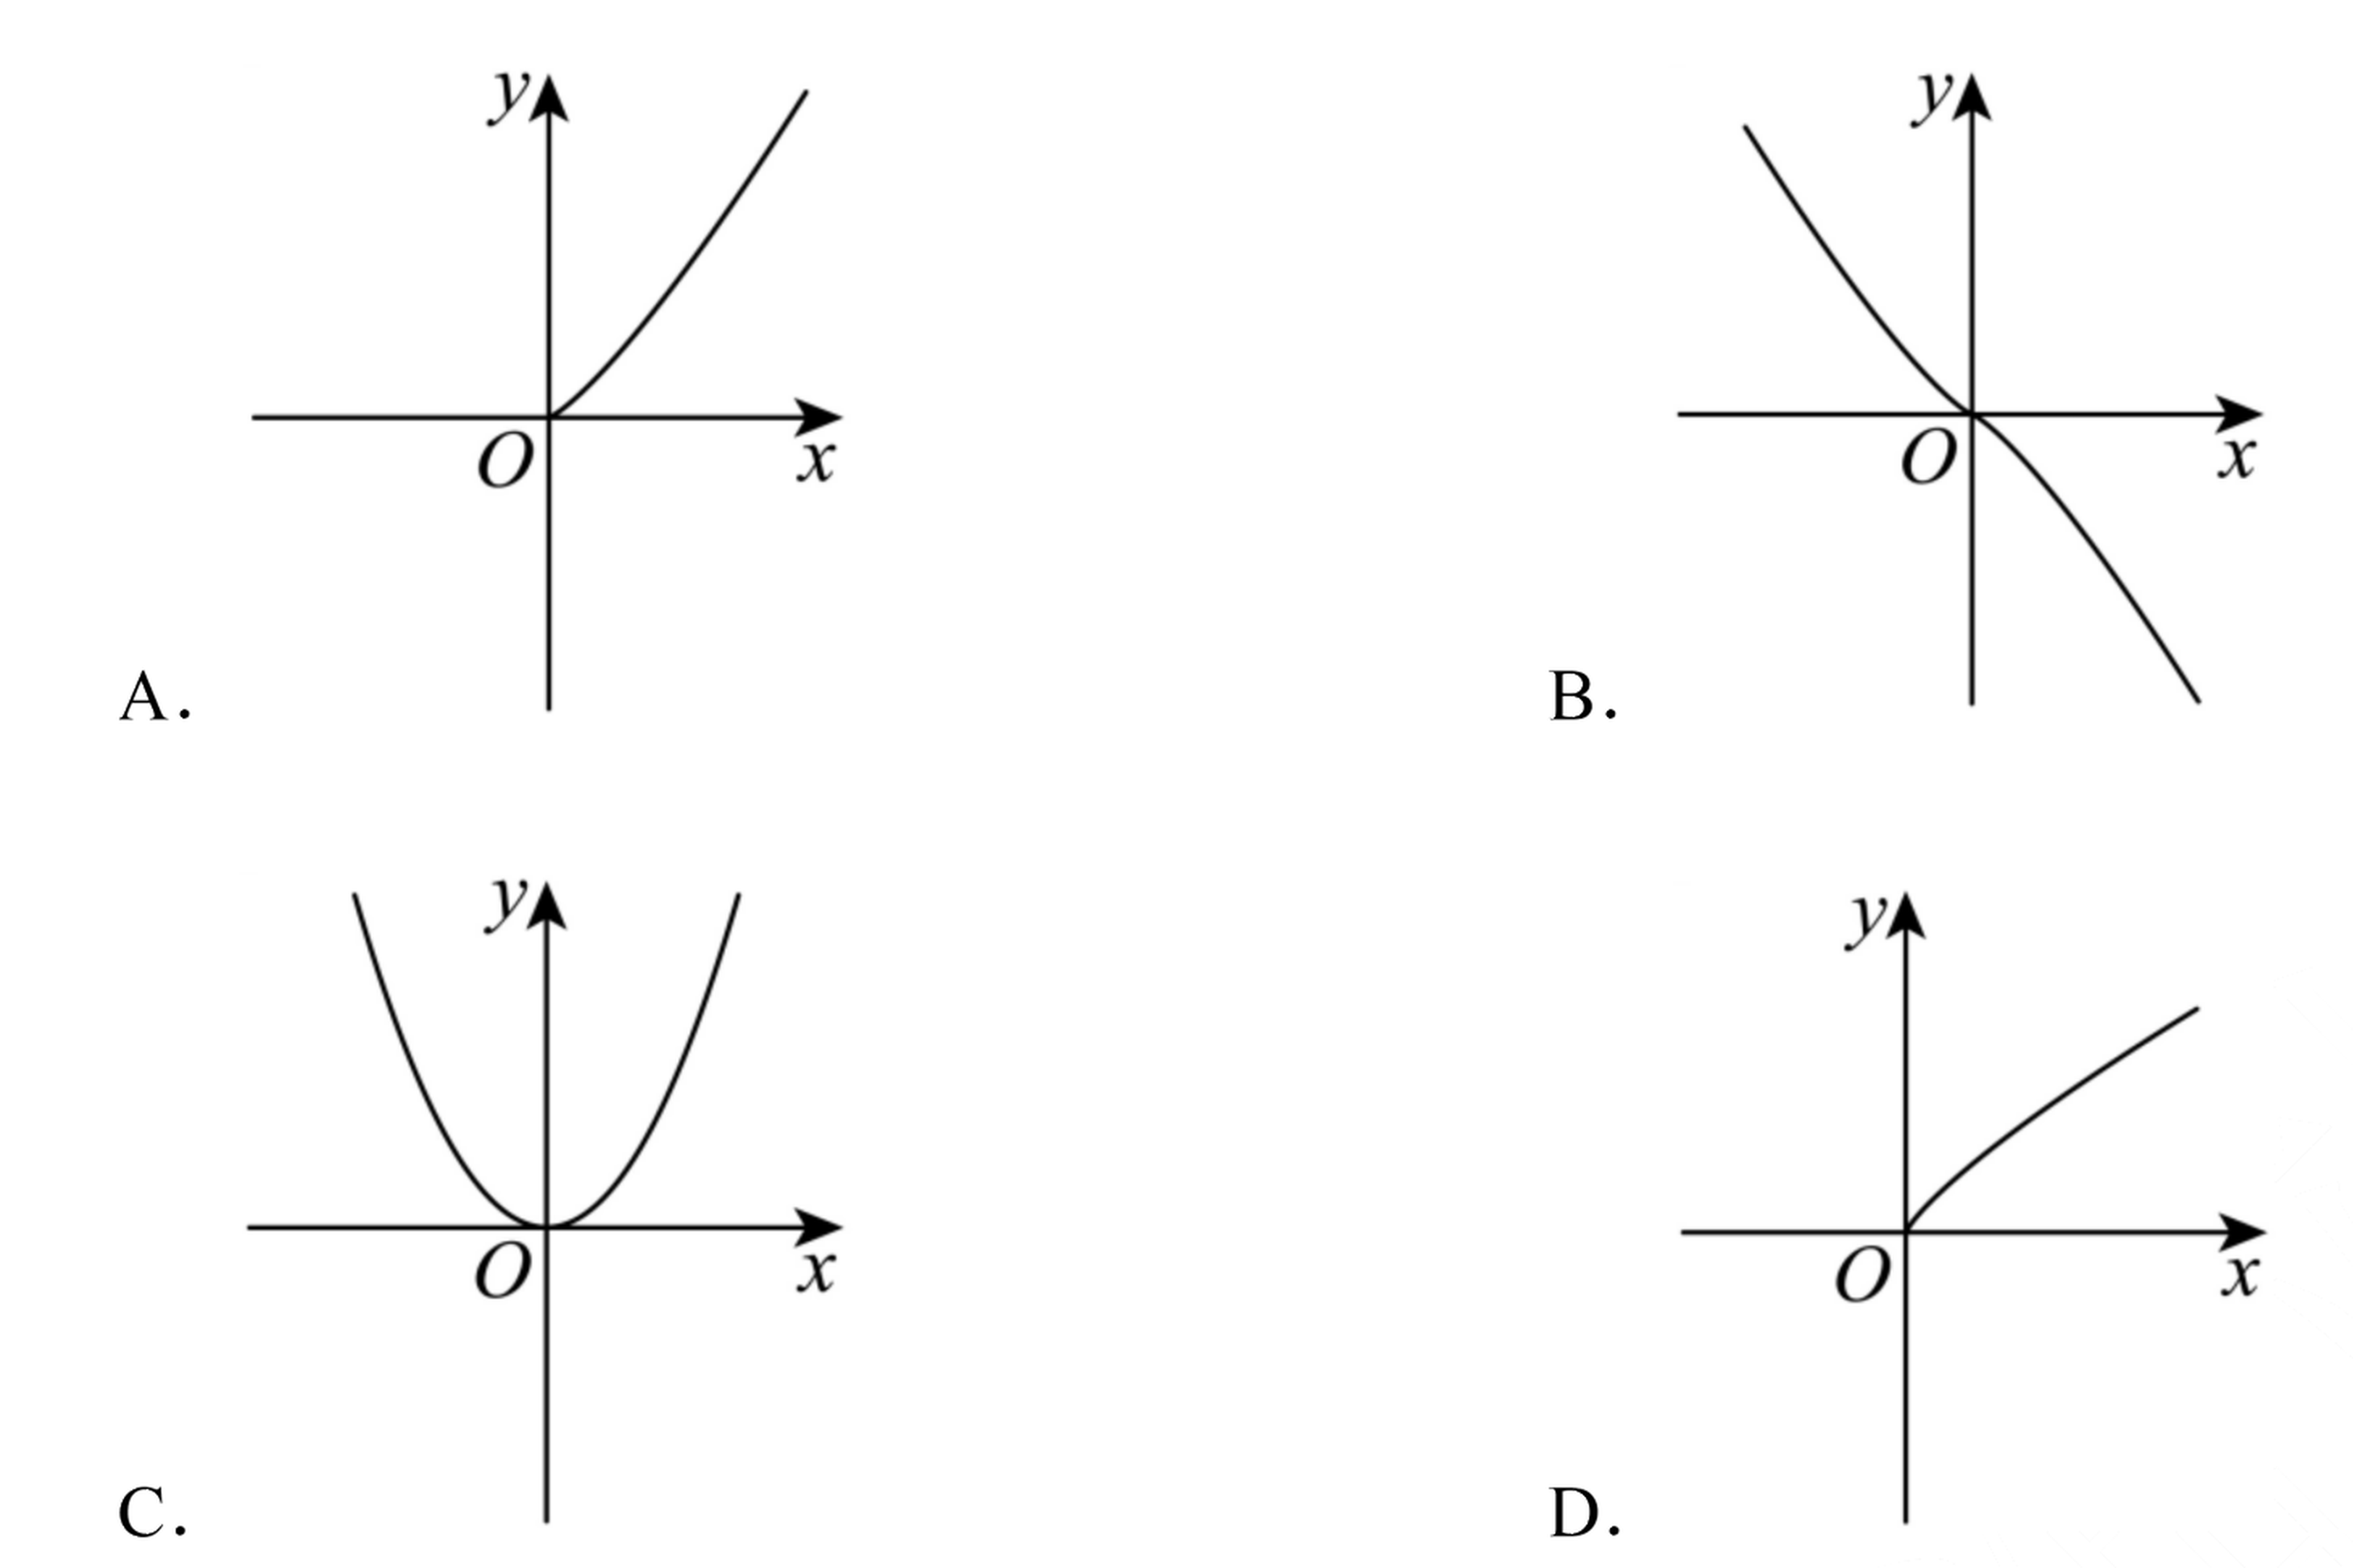
\includegraphics[width=0.80\textwidth]{figures/gao136_q13.png}
\end{center}

\ifanswer
\solbegin
\step{由 $y=x^{\frac54}=\sqrt[4]{x^5}$，函数的定义域为 $[0,+\infty)$，排除 BC，}% 原卷"排除 BC"连写，照录
\step{因为 $\dfrac54>1$，所以函数 $y=x^{\frac54}$ 的图象呈现下凸的趋势，排除 D. 故选 $A$.}
\solend
\fi

\item 下列不等式① $a+\dfrac1a\geqslant2$；② $a^2+4\geqslant4a$；③ $\left\lvert\dfrac ba+\dfrac ab\right\rvert\geqslant2$；④ $\dfrac{2a^2b^2}{a^2+b^2}\leqslant ab$；其中恒成立的是\mbox{（\quad）}

\keepwithprev
A. ①④\qquad B. ③④\qquad C. ②③\qquad D. ①②

\ifanswer
\ans{$C$}
\fi

\item 函数 $y=a^x+b-1(a>0,a\neq1)$ 单调递增且图象不经过第四象限，则 $a,b$ 满足的条件为\mbox{（\quad）}

\keepwithprev
A. $a>1,b\leqslant1$\qquad B. $a>1,b\geqslant0$\qquad C. $0<a<1,b\leqslant1$\qquad D. $0<a<1,b\geqslant1$

\ifanswer
\solbegin
\step{因为函数 $y=a^x+b-1$ 单调递增，所以 $a>1$，}
\step{图象不经过第四象限，则 $x=0$ 时，$y=b\geqslant0$，所以 $a>1,b\geqslant0$，故选 $B$.}
\solend
\fi

\item 设关于 $x$ 的不等式 $\dfrac{ax-1}{x^2-a}<0$ 的解集为 $S$，且 $3\in S$，$4\notin S$，则实数 $a$ 的取值范围为\mbox{（\quad）}

\keepwithprev
A. $(-\infty,-\sqrt3)\cup\left(\dfrac13,\sqrt3\right)$\qquad B. $\left(-\infty,\dfrac14\right)\cup(16,+\infty)$

C. $\left[\dfrac14,\dfrac13\right)\cup(9,16]$\qquad D. 不能确定

\ifanswer
\solbegin
\step{若 $3\in S$，则 $\dfrac{3a-1}{9-a}<0$，解得 $a\in\left(-\infty,\dfrac13\right)\cup(9,+\infty)$，}
\step{若 $4\notin S$，则 $16-a=0$ 或 $\dfrac{4a-1}{16-a}\geqslant0$，解得 $a\in\left[\dfrac14,16\right]$，}
\step{故实数 $a$ 的取值范围为 $\left[\dfrac14,\dfrac13\right)\cup(9,16]$，故选 $C$.}
\solend
\fi

\end{enumerate}

\bigsec{三、解答题}

\begin{enumerate}
\setcounter{enumi}{16}

\item 计算：(1) 计算 $\dfrac{\lg8+\lg125-\lg2-\lg5}{\lg\sqrt{10}\cdot\lg0.1}$；(2) 若 $a^{2x}=2(a>0)$，求 $\dfrac{a^{3x}+a^{-3x}}{a^x+a^{-x}}$.

\ifanswer
\solbegin
\step{(1) 原式 $=\dfrac{2-1}{\frac12\cdot(-1)}=-2$；(2) 原式 $=a^{2x}-1+a^{-2x}=2-1+\dfrac12=\dfrac32$.}
\solend
\fi

\item 不等式 $\dfrac{x-1}{x+1}\geqslant0$ 的解集为 $A$，不等式 $(x-a-1)(2a-x)>0(a<1)$ 的解集为 $B$.

(1) 求集合 $A$；

(2) 若 $B\subseteq A$，求实数 $a$ 的取值范围.

\ifanswer
\solbegin
\step{(1) $A=(-\infty,-1)\cup[1,+\infty)$.}
\step{(2) 由 $(x-a-1)(2a-x)>0(a<1)$，得 $(x-a-1)(x-2a)<0(a<1)$，}
\step{因为 $a<1$，所以 $a+1>2a$，所以 $B=(2a,a+1)$，}
\step{因为 $B\subseteq A$，所以 $2a\geqslant1$ 或 $a+1\leqslant-1$，即 $a\geqslant\dfrac12$ 或 $a\leqslant-2$，}
\step{而 $a<1$，所以实数 $a$ 的取值范围 $(-\infty,-2]\cup\left[\dfrac12,1\right)$.}% 原卷"取值范围"后脱"是／为"，照录
\solend
\fi

\item 已知幂函数 $y=x^m(m\in\R)$ 经过点 $\left(4,\dfrac12\right)$.

(1) 求此幂函数的表达式和定义域；

(2) 已知点 $A(a+2,y_1)$，点 $B(3-2a,y_2)(a\in\R)$ 在此幂函数的图像上，且满足 $y_1<y_2$，求实数 $a$ 的取值范围.

\ifanswer
\solbegin
\step{(1) 幂函数 $y=x^m(m\in\R)$ 经过点 $\left(4,\dfrac12\right)$，所以 $4^m=\dfrac12\Rightarrow m=-\dfrac12$，}
\step{所以 $f(x)=x^{-\frac12}$，定义域为 $(0,+\infty)$.}
\step{(2) 由于函数 $f(x)$ 在其定义域 $(0,+\infty)$ 上严格减，}
\step{由 $y_1<y_2$，得 $a+2>3-2a\geqslant0\Rightarrow a\in\left(\dfrac13,\dfrac32\right]$.}
\solend
\fi

% 第 20 题图取 05 页截图（0.42\textwidth、高约 6cm）。试排 \item 前加 7cm 守卫会多出
% 一张只有两行正文的稀疏页，且三版不加守卫时图均与题干、【解析】同页，故不另加守卫
\item 某医药研究所开发一种抗甲流新药，如果成年人按规定的剂量服用，据监测：服药后每毫升血液中的含药量 $y$（微克）与时间 $t$（小时）之间近似满足如图所示的曲线.

(1) 结合图，求 $k$ 与 $a$ 的值；

(2) 写出服药后 $y$ 与 $t$ 之间的函数关系式 $y=f(t)$；

(3) 据进一步测定：每毫升血液中含药量不少于 $0.5$ 微克时治疗疾病有效，求服药一次治疗有效的时间范围？

\begin{center}
% 图取原卷 05 页截图去粉色水印、去色，3x LANCZOS 放大
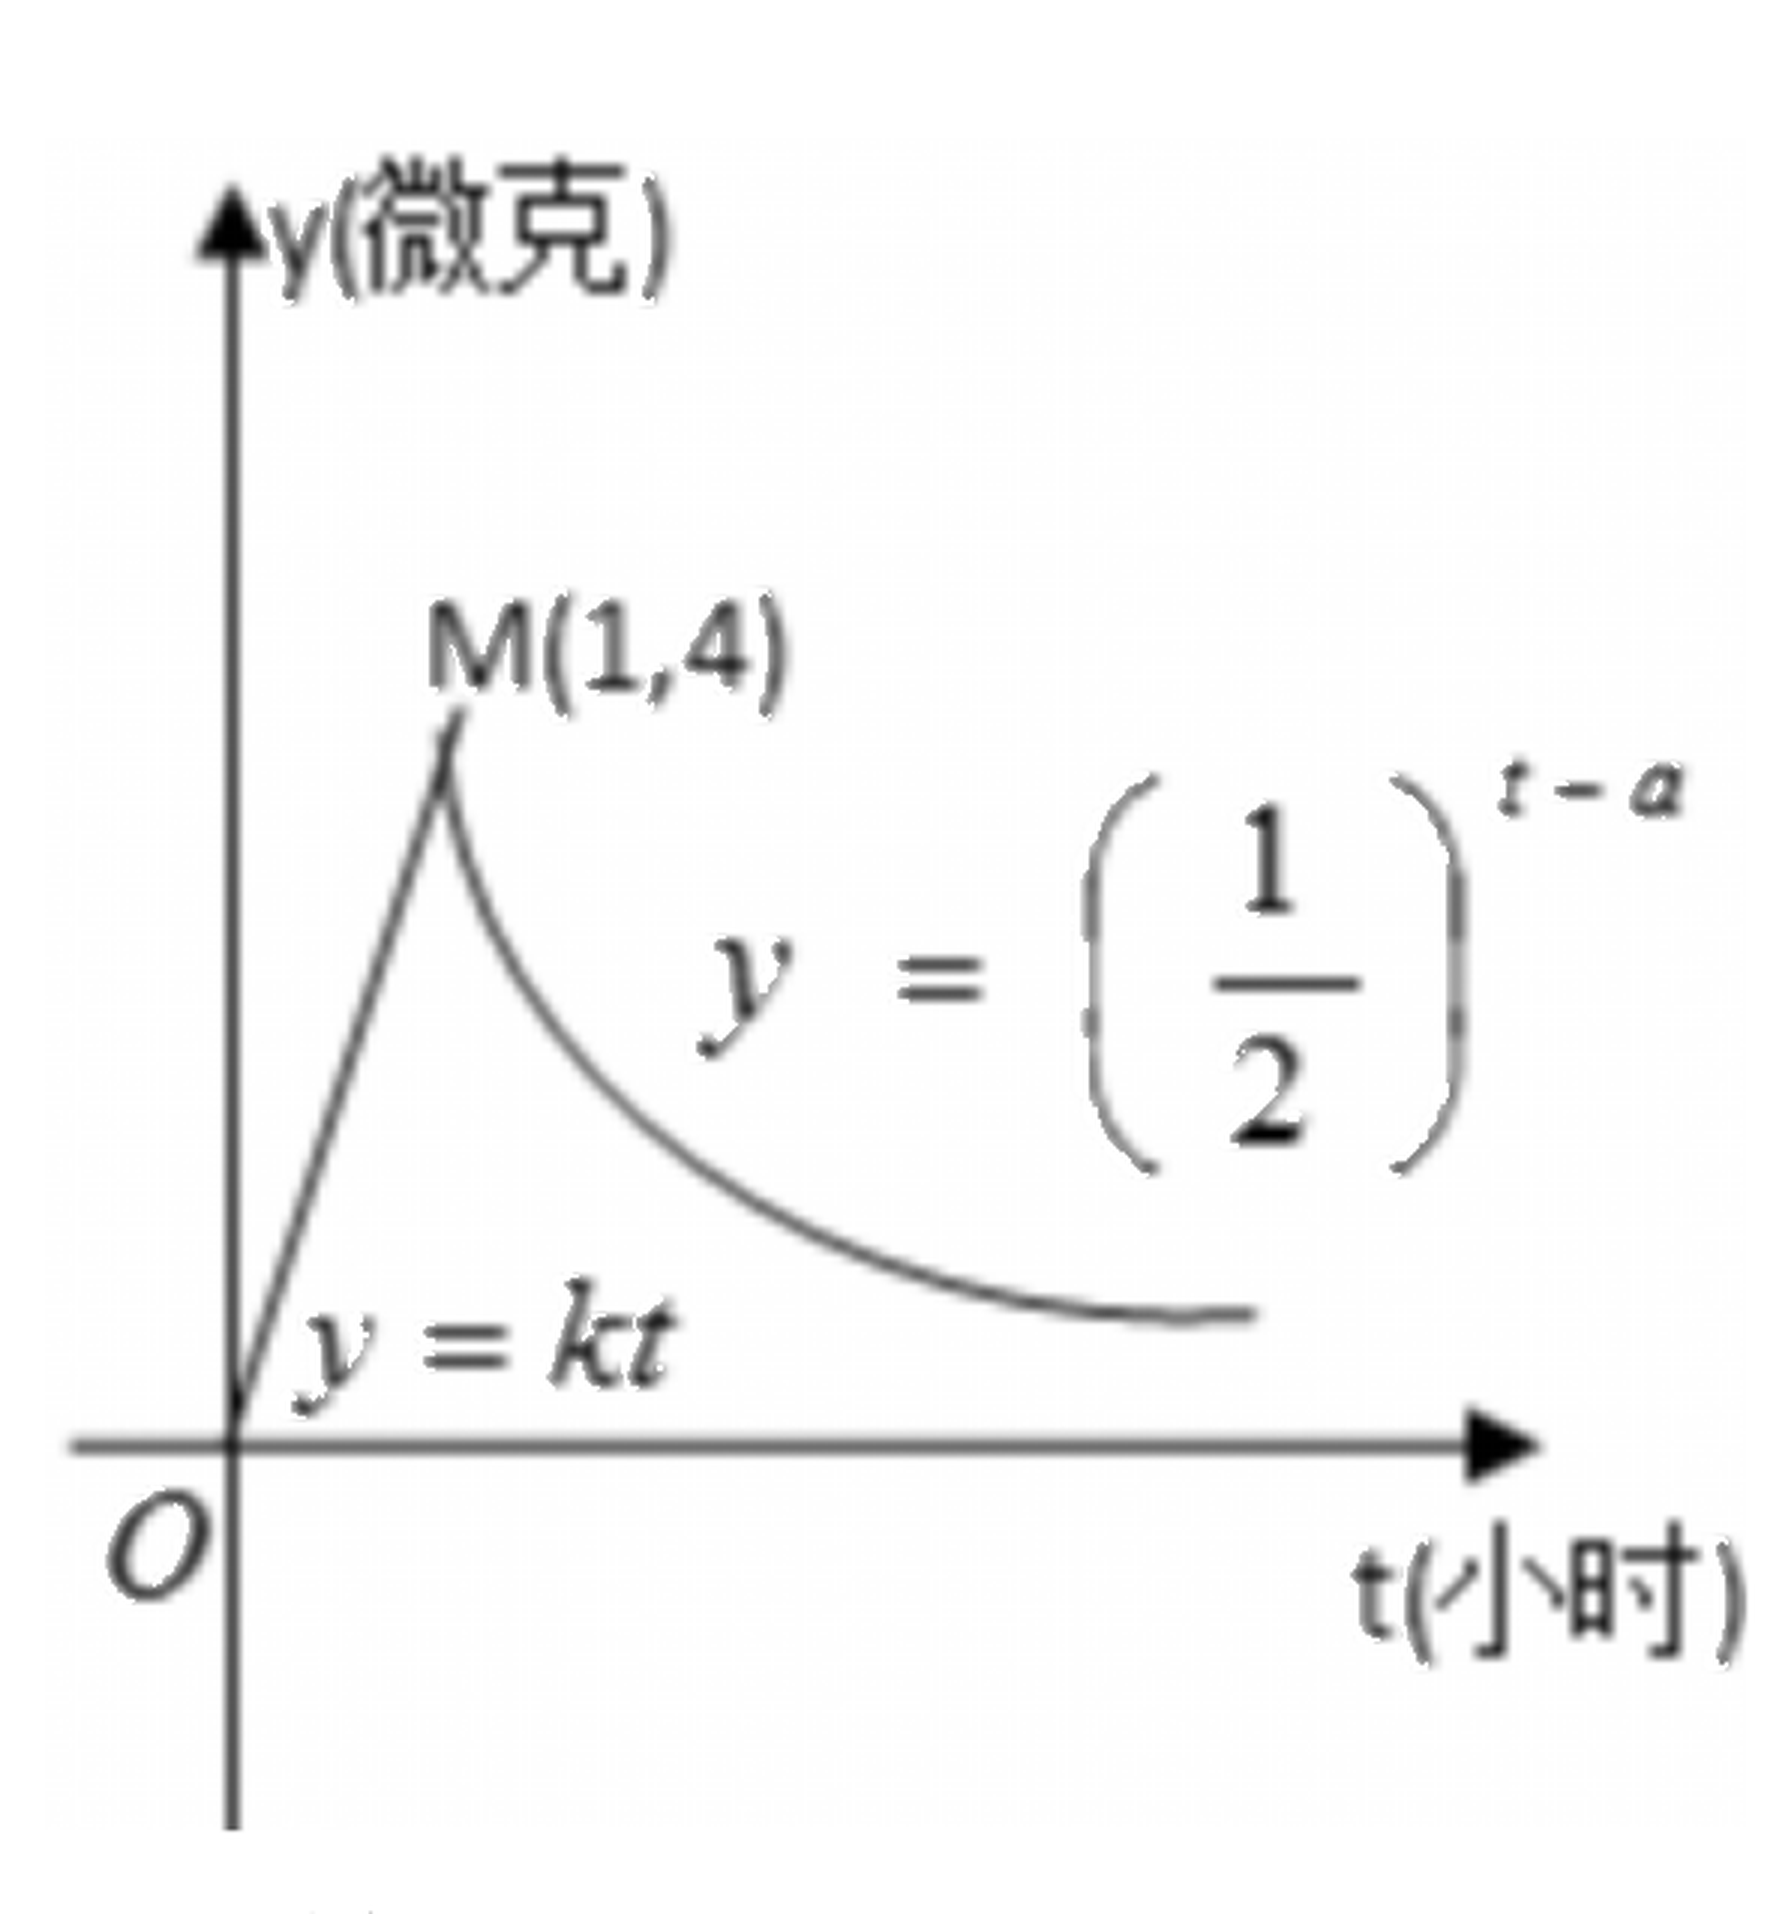
\includegraphics[width=0.42\textwidth]{figures/gao136_q20.png}
\end{center}

\ifanswer
\solbegin
\step{(1) 当 $0\leqslant t\leqslant1$ 时，函数图象是一条线段，由于过原点与点 $(1,4)$，所以 $k=4$，}
\step{其解析式为 $y=4t$，$0\leqslant t\leqslant1$；}
\step{当 $t\geqslant1$ 时，函数的解析式为 $y=\left(\dfrac12\right)^{t-a}$，}
\step{此时 $M(1,4)$ 在曲线上，将此点的坐标代入函数解析式得 $4=\left(\dfrac12\right)^{1-a}$，}
\step{解得 $a=3$；}
\step{(2) 由 (1) 得 $f(t)=\begin{cases}4t,0\leqslant t\leqslant1\\\left(\frac12\right)^{t-3},t>1\end{cases}$；}
\step{(3) 由 (2) 得，令 $f(t)\geqslant0.5$，即 $\begin{cases}4t\geqslant0.5,0\leqslant t\leqslant1\\\left(\frac12\right)^{t-3}\geqslant0.5,t>1\end{cases}$，所以 $\dfrac18\leqslant t\leqslant4$.}
\solend
\fi

\item 已知关于 $x$ 的不等式 $(kx-k^2-4)(x-4)>0$，其中 $k\in\R$.

(1) 当 $k=-1$，求不等式的解集 $A$；

(2) 当 $k$ 变化时，试求不等式的解集 $A$；

(3) 对于不等式解集 $A$，满足 $A\cap\Z=B$. 试探究集合 $B$ 能否为有限集，若能，求出使得集合 $B$ 中元素最少的 $k$ 的所有取值，并用列举法表示此时的集合 $B$，若不能，说明理由；

\ifanswer
\solbegin
\step{(1) 当 $k=-1$ 时，原不等式可化为 $(x+5)(x-4)<0$，}
\step{解得 $-5<x<4$，故不等式的解集为 $\{x\mid -5<x<4\}$；}
\step{(2) 当 $k=0$ 时，解集为 $\{x\mid x<4\}$，}
\step{当 $k>0$ 时，$\dfrac{k^2+4}{k}=k+\dfrac4k\geqslant4$，解集为 $\{x\mid x<4\text{ 或 }x>\dfrac{k^2+4}{k}\}$；}
\step{当 $k<0$ 时，解集为 $\{x\mid \dfrac{k^2+4}{k}<x<4\}$，}
\step{综上，当 $k=0$ 时，$A=\{x\mid x<4\}$，}
\step{当 $k>0$ 时，$A=\{x\mid x<4\text{ 或 }x>\dfrac{k^2+4}{k}\}$；}
\step{当 $k<0$ 时，$A=\{x\mid \dfrac{k^2+4}{k}<x<4\}$，}
\step{(3) 由 (2) 得当 $k\geqslant0$ 时，$B$ 为无限集，当 $k<0$ 时，$B$ 为有限集，}
\step{此时，$\dfrac{k^2+4}{k}=k+\dfrac4k\leqslant-4$，当且仅当 $k=-2$ 时取等号，}
\step{所以 $k=-2$ 时，$B$ 中元素最少，此时 $A=\{x\mid -4<x<4\}$，}
\step{所以 $B=\{-3,-2,-1,0,1,2,3\}$.}
\solend
\fi

\end{enumerate}

% 第 22 题是"四、附加题"首题且带 9cm 图块，守卫须放在 \bigsec 之前连节标题一起量，
% 否则"四、附加题"会孤立在页末（B 类，照 高一26／40／59 成例）
\needvspace{11cm}
\bigsec{四、附加题}

\begin{enumerate}
\setcounter{enumi}{21}

% 第 22 题四幅抛物线/坐标图选项是一整块，守卫放在 \item 之前
\needvspace{9cm}
\item 函数 $f(x)=\left(\dfrac12\right)^{\lvert x+1\rvert}$ 的图象大致为\mbox{（\quad）}

\keepwithprev
\begin{center}
% 四幅抛物线/坐标图选项取原卷 07 页截图去粉色水印，按原卷 2x2 排布合并为一张
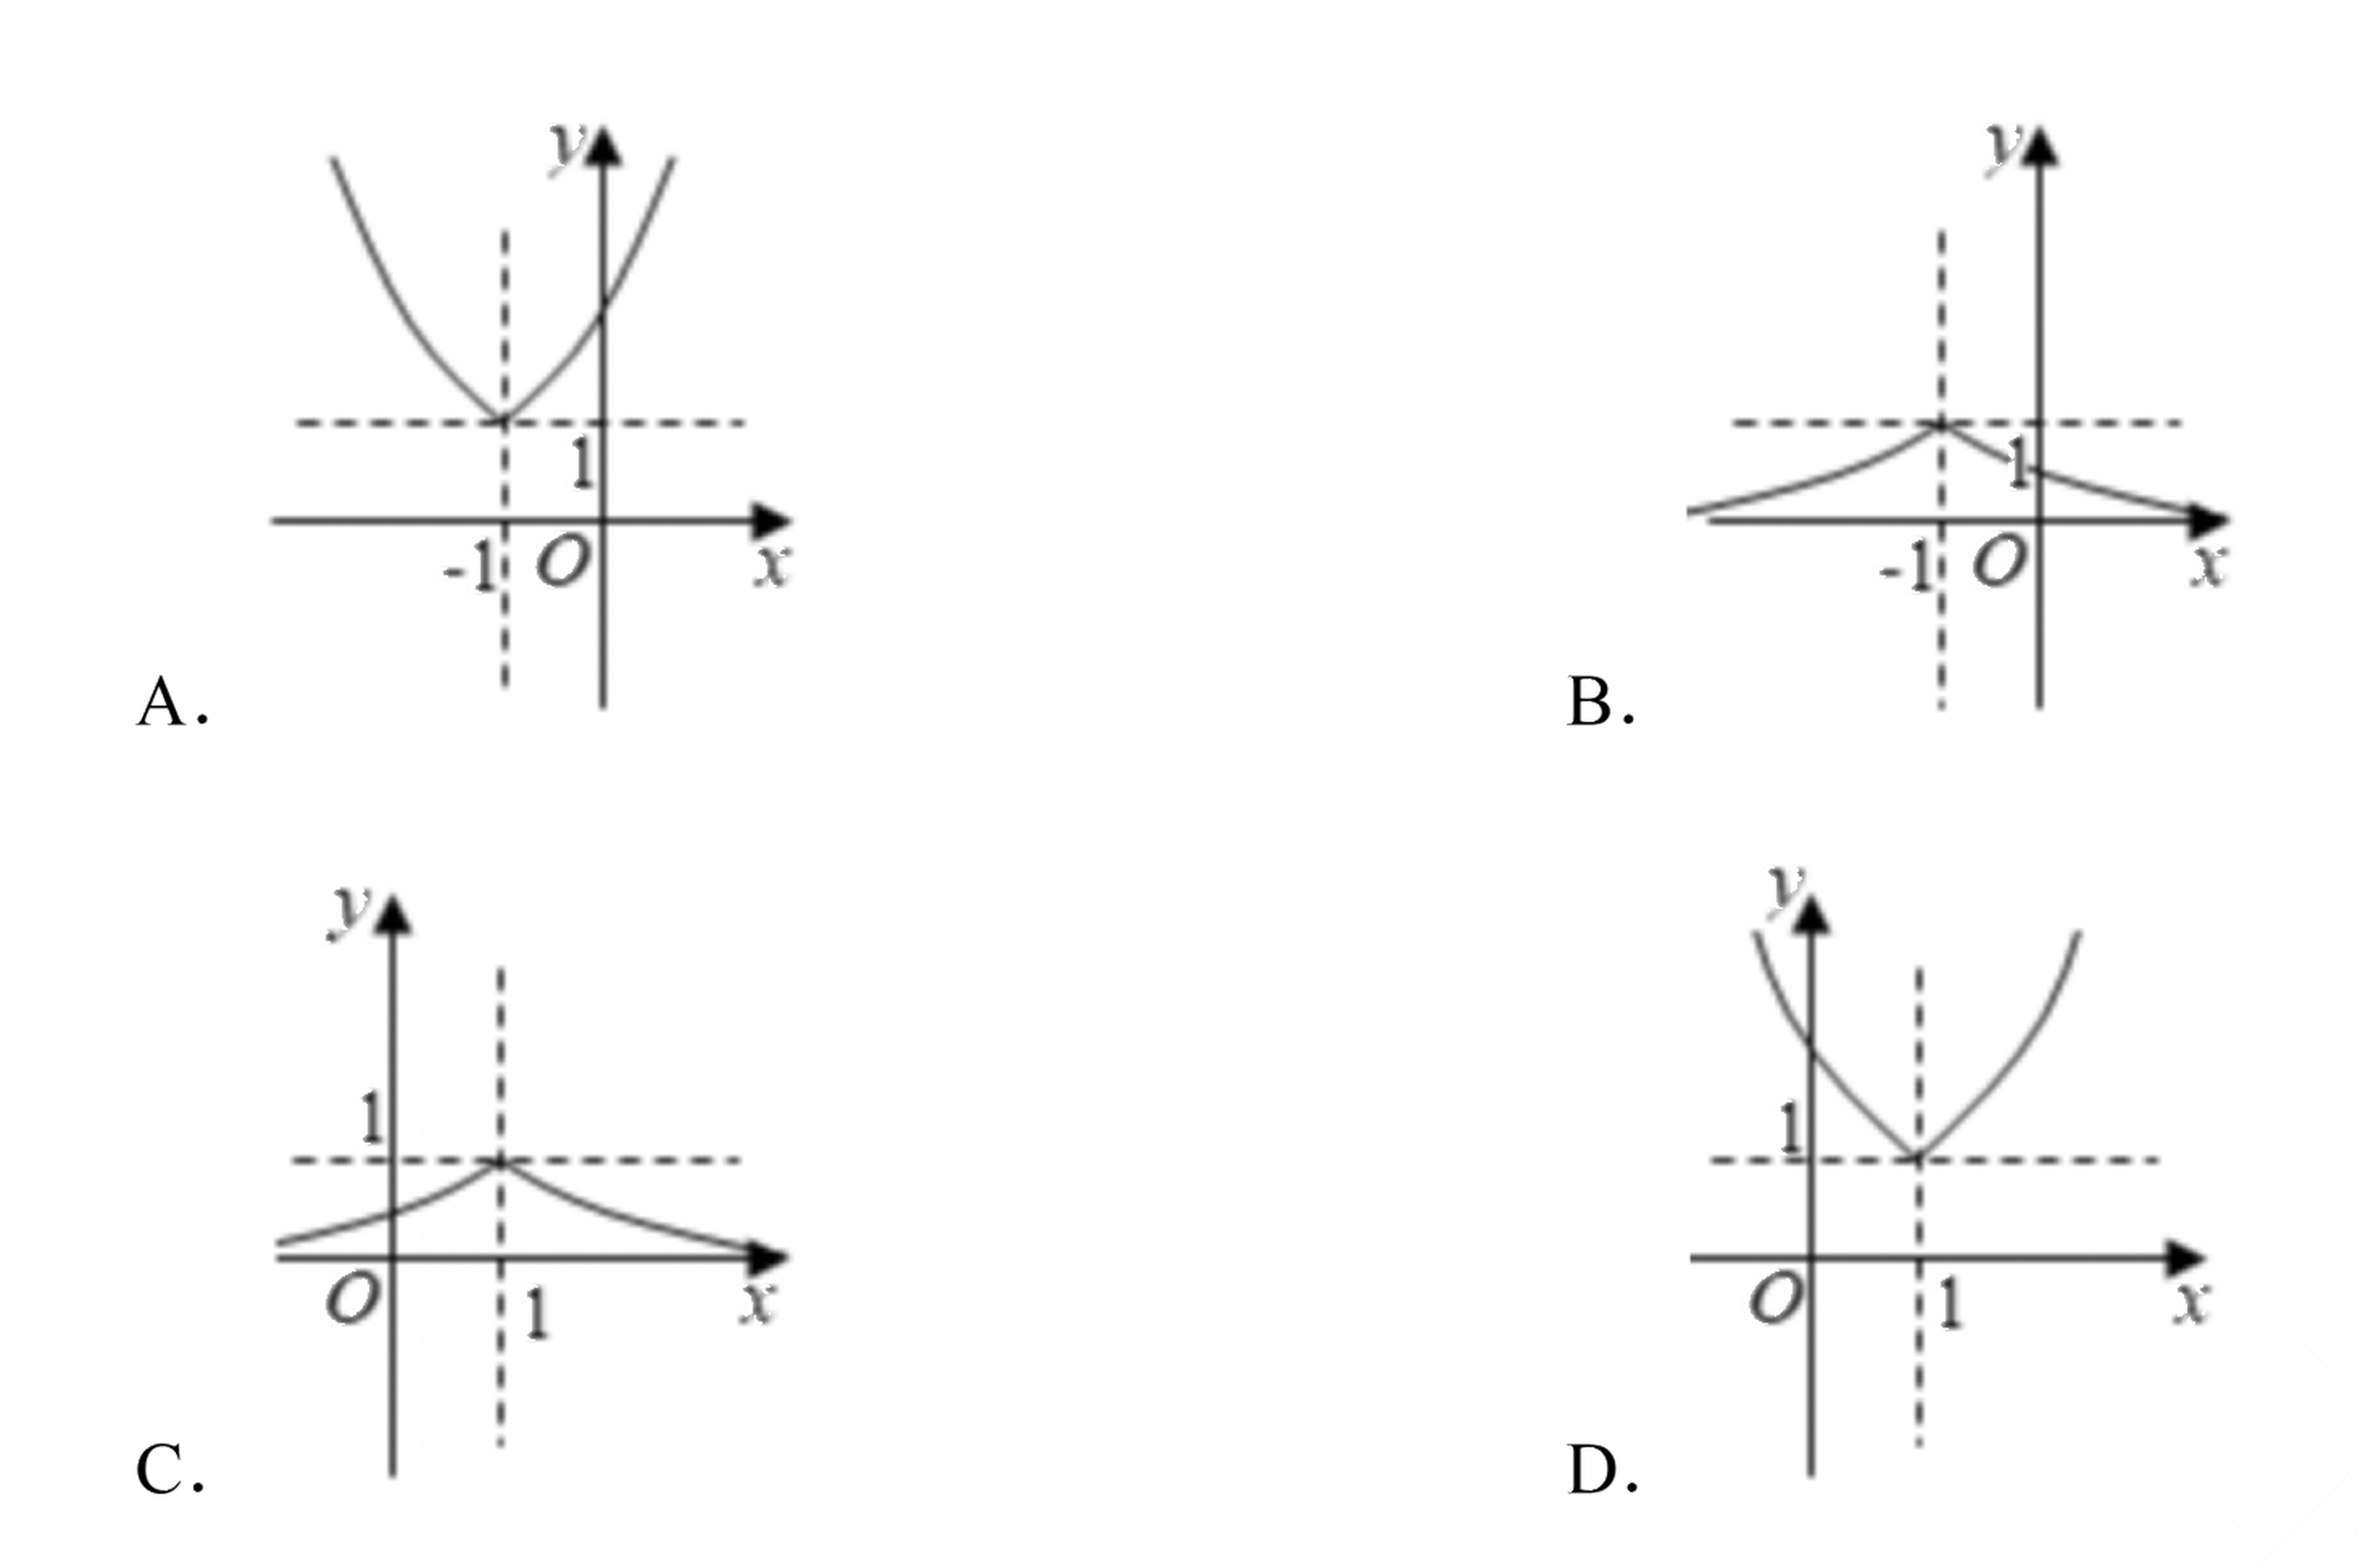
\includegraphics[width=0.80\textwidth]{figures/gao136_q22.png}
\end{center}

\ifanswer
\ans{$B$}
\fi

\end{enumerate}

\end{document}
"
% 紧凑版：xelatex "\def\iscompact{1}% 高一136_三林中学_期中.tex
%   —— 高一上数学"2026-2027 年三林中学高一上期中"（试卷版/答案版）
% 试卷版：xelatex 高一136_三林中学_期中.tex
% 答案版：xelatex "\def\isanswer{1}\input{高一136_三林中学_期中.tex}"
% 紧凑版：xelatex "\def\iscompact{1}\input{高一136_三林中学_期中.tex}"
%
% ① 原始材料：微信公众号"魔都数学加油站"文章，作者破晓，2026-11-15 18:04 发布；
% 连载"27学年高一136"，原文标题"27学年高一136——2026-2027年上海市三林中学高一上期中"；
% 原文链接：https://mp.weixin.qq.com/s/jaMzqMm6pDvcT0yM0d7eaQ。
% 正文为 7 张 PNG 页（01、04、06 为 4762x6735；02、03、05、07 为 2560x3620，
% 同一篇各页分辨率不同，逐页按各自分辨率裁图核对），题目下印有【答案】或【解析】，为讲评版。
% 题目、解析均据原图转录；卷面粉红色水印"魔都数学加油站"及公众号页脚未录入。
% 全卷 3 幅插图：第 13 题四幅坐标图选项（03 页）、第 20 题药物浓度折线/曲线图（05 页）、
% 第 22 题四幅抛物线/坐标图选项（07 页），均取原卷截图去粉色水印、去色、LANCZOS 放大，
% 四幅选项按原卷 2x2 排布合并为一张；图前按惯例加 \needvspace 守卫。
%
% 卷首标题：原卷印作"2026-2027 年三林中学高一上期中"（公众号标题中的"上海市"
% 卷面标题行没有，本稿照卷面），年份区间按全稿惯例排 en dash；原卷未印副标题，
% 本卷为期中卷、跨集合与常用逻辑用语／不等式／函数三章，按题目内容标为
% "集合与常用逻辑用语、不等式、函数"（与 125／126／128／129／131／132／133 同期中卷口径相同）：
% 集合与逻辑见 Q3、Q6、Q10、Q12、Q16、Q18、Q21，不等式见 Q5、Q7、Q8、Q9、Q14、Q15，
% 函数（幂函数、指数／对数、基本不等式应用）见 Q4、Q11、Q13、Q17、Q19、Q20、Q22。
%
% 题号体例：本卷共 20 题——一、填空题 3—12（10 题）、二、选择题 13—16（4 题）、
% 三、解答题 17—21（5 题）、四、附加题 22（1 题）。四节分别
% \setcounter{enumi}{2}／{12}／{16}／{21}。
%
% ② 与原卷的排版差异：
%   ① 原文从第 3 题起，本稿保留原题号；末节"四、附加题"另起 \bigsec，题号续到 22；
%   ② 原卷每题下直接印【答案】或【解析】，本稿按全稿惯例置于答案版；第 3、4、6 题只印
%      【答案】、无【解析】，提 \ans{}；第 14 题答案 C 印在题干括号内、无【解析】，按
%      高一53／高一108／高一132／高一133 成例括号留空、另提 \ans{$C$}；第 22 题答案 B
%      印在题干括号内、无【解析】，同例提 \ans{$B$}；第 13、15、16 题答案在解析末句
%      "故选 …"，括号内留空、不另提 \ans{}；其余各题印【解析】、无独立答案段；
%   ③ 原卷未印副标题，本稿按"知识模块"口径补出；
%   ④ 原卷填空横线按全稿惯例排为 \blankline[4.4em]；选择题括号排 \mbox{（\quad）}、
%      每个选项段前按惯例加 \keepwithprev（四幅图选项那一枚放在 \begin{center} 之前）；
%      解答题不留作答区、不加 \anspace（原卷为讲评版，与 129／131／132／133 同）；
%   ⑤ 原卷数集排斜体 $R$／$R^+$／$Z$，按全稿惯例改 \R／\R^+／\Z；空集记号 \varnothing；
%      绝对值排 \lvert…\rvert，集合描述竖线排 \mid；不等号按全稿惯例排 \leqslant／\geqslant；
%   ⑥ 子题标号 (1)(2)(3) 原卷用半角括号，照录；圈数字 ①②③④ 照录；第 12 题甲／乙／丙
%      三行与第 14 题四个编号不等式照录；
%   ⑦ 数学式内半角逗号照录（如 Q4"$a>0,a\neq1$"、Q6"$\{(-2,4),(1,1)\}$"、
%      Q7"$a=2+3=5,b=2\times3=6$"、Q11"$x_1,x_2$"、Q12"$m,n\in R^+$"、
%      Q15"$a>1,b\geq0$"、Q18"$B=(2a,a+1)$"、Q20"$4t,0\leq t\leq1$"、
%      Q21"$\{-3,-2,-1,0,1,2,3\}$"）；原卷行末西文句点照录，行中全角逗号照录；
%   ⑧ 三幅插图：第 13 题四幅坐标图选项合并裁为一张 \includegraphics（题前 \needvspace{9cm}）；
%      第 20 题折线/曲线图取 05 页截图（0.42\textwidth）；第 22 题四幅抛物线/坐标图选项合并
%      裁为一张（题前 \needvspace{9cm}）。第 13、22 题分别是"二、选择题""四、附加题"的首题
%      且带大图块，另在两处 \bigsec 之前各加 \needvspace{11cm} 连节标题一起量，避免节标题
%      孤立在页末（切页审计 B 类；照 高一26／40／59 成例）。第 20 题图不是节首题、三版试排
%      图均与题干同页，加 7cm 守卫反会多出一张只有两行正文的稀疏页，故不另加守卫；
%      三版切页审计均"合计异常：无"（试卷 4 页／紧凑 4 页／答案 6 页）；
%   ⑨ 跨页续印按题合并：Q16 题干在 03 页、括号与选项及【解析】在 04 页；Q19 题干在 04 页、
%      (2) 与【解析】在 05 页；Q20 (3)【解析】在 06 页；Q22 四幅图在 07 页；本稿按题连排；
%   ⑩ 题干中的中文弯引号按原卷照录，注释内一律 ASCII 引号；原卷"图像／图象"两种写法混用，
%      逐处照录（Q4、Q19 作"图像"，Q13、Q15、Q20、Q22 作"图象"）；
%   ⑪ 附加题节：原卷印"四、附加题"，本稿用 \bigsec{四、附加题} 另起一节、
%      \setcounter{enumi}{21}，顶层 1 个 \item（与 高一09／15／16／22／35／39／47／61 同口径）；
%      Q22 只印括号内答案、提 \ans{}，不计入 \step 账。
%
% 判别式字形：全卷仅第 9 题【解析】cases 块出现判别式"$\Delta=a^2-8a<0$"，原卷印
%   等腰、偏高的三角 $\Delta$，逐处放大核对并照录 \Delta；全卷未出现扁等边三角 \triangle。
%
% 子集符号：第 18 题 (2) 题干"$B\subseteq A$"与【解析】"$B\subseteq A$"两处原卷均印
%   带下划线 $\subseteq$，逐处放大核对、照录 \subseteq；全卷未出现单线 \subset。
%
% 原卷存疑照录（均照录未改，正文对应处另有 % 注）：
%   第 12 题乙行"$\dfrac{m+n}{mm}=\dfrac1{mn}$"前一分母印作 $mm$（后一处作 $mn$），照录；
%   第 12 题【解析】"$\geqslant\dfrac1{100}\left[a^2+1+2\sqrt{a^2}\right]$"保留 $\sqrt{a^2}$
%      未化简为 $a$，照录；
%   第 13 题【解析】"排除 BC"与"排除 D"连写选项字母，照录；
%   第 18 题 (2)【解析】末行"所以实数 $a$ 的取值范围 $(-\infty,-2]\cup[\frac12,1)$"
%      "取值范围"后脱"是／为"字，照录；
%   第 21 题 (3) 题干"求出使得集合 $B$ 中元素最少的 $k$ 的所有取值"而【解析】只给出
%      $k=-2$ 一处，措辞照录。
%
% 行数复核：逐题数 \step 条数，合计 51 条（Q3：0；Q4：0；Q5：2；Q6：0；Q7：2；Q8：1；
% Q9：1；Q10：4；Q11：1；Q12：4；Q13：2；Q14：0；Q15：2；Q16：3；Q17：1；Q18：5；
% Q19：4；Q20：7；Q21：12；Q22：0），与原卷印刷行逐题相等（cases 块作一个印刷行计）。
% 第 3、4、6、14、22 题只印【答案】、提 \ans{}，不计入 \step 账；第 13、15、16 题答案在
% 解析末句，括号内留空、不另提 \ans{}。
%
\documentclass[a4paper,11pt]{article}
\usepackage{common}

\begin{document}

\examtitlest[3]{2026--2027 年三林中学高一上期中}{集合与常用逻辑用语、不等式、函数}

\bigsec{一、填空题}

\begin{enumerate}
\setcounter{enumi}{2}

\item 用反证法证明命题“若 $x+y\neq5$，则 $x\neq2$ 或 $y\neq3$”为真命题时，第一个步骤是\blankline[4.4em].

\ifanswer
\ans{假设 $x=2$ 且 $y=3$}
\fi

\item 函数 $y=a^{x-1}+1(a>0,a\neq1)$ 的图像恒过定点 $A$，则点的坐标是\blankline[4.4em].

\ifanswer
\ans{$(1,2)$}
\fi

\item 已知 $x>1$，则 $x+\dfrac4{x-1}$ 的最小值是\blankline[4.4em].

\ifanswer
\solbegin
\step{由 $x>1$，得 $x-1>0$，则 $x+\dfrac4{x-1}=x-1+\dfrac4{x-1}+1\geqslant2\sqrt{(x-1)\cdot\dfrac4{x-1}}+1=5$，}
\step{当且仅当 $x-1=\dfrac4{x-1}$ 即 $x=3$ 时取等号，取得最小值 $5$.}
\solend
\fi

\item 已知集合 $A=\{(x,y)\mid y=x^2\}$，集合 $B=\{(x,y)\mid y=2-x\}$，求 $A\cap B=$\blankline[4.4em].

\ifanswer
\ans{$\{(-2,4),(1,1)\}$}
\fi

\item 已知一元二次不等式 $x^2-ax+b<0$ 的解集为 $(2,3)$，则不等式 $bx^2-ax+1>0$ 的解集是\blankline[4.4em].

\ifanswer
\solbegin
\step{$a=2+3=5,b=2\times3=6$，则 $bx^2-ax+1>0$ 即 $6x^2-5x+1>0$，}
\step{即 $(3x-1)(2x-1)>0$，解集为 $\left(-\infty,\dfrac13\right)\cup\left(\dfrac12,+\infty\right)$.}
\solend
\fi

\item 不等式 $(x+2)^3<(5-2x)^3$ 的解集为\blankline[4.4em].

\ifanswer
\solbegin
\step{由 $(x+2)^3<(5-2x)^3$ 得 $x+2<5-2x$，故解集为 $(-\infty,1)$.}
\solend
\fi

\item 若关于 $x$ 的不等式 $ax^2-ax+2>0$ 的解集为 $\R$，则实数 $a$ 的取值范围是\blankline[4.4em].

\ifanswer
\solbegin
\step{由题意得 $a=0$ 或 $\begin{cases}a>0\\\Delta=a^2-8a<0\end{cases}$，所以 $0\leqslant a<8$.}% 判别式原卷印高三角 $\Delta$，照录
\solend
\fi

\item 已知关于 $x$ 的不等式 $\lvert x+3\rvert+\lvert x-a\rvert\geqslant5$ 恒成立，则实数 $a$ 的取值范围为\blankline[4.4em].

\ifanswer
\solbegin
\step{因为 $\lvert x+3\rvert+\lvert x-a\rvert\geqslant\lvert x-a-x-3\rvert=\lvert 3+a\rvert$，}
\step{要使 $\lvert x+3\rvert+\lvert x-a\rvert\geqslant5$ 恒成立，则 $\lvert a+3\rvert\geqslant5$ 即可，}
\step{所以 $a+3\geqslant5$ 或 $a+3\leqslant-5$，解得 $a\geqslant2$ 或 $a\leqslant-8$，}
\step{即实数 $a$ 的取值范围是 $(-\infty,-8]\cup[2,+\infty)$.}
\solend
\fi

\item 若方程 $\lg^2 x-2\lg x-2=0$ 的两个解为 $x_1,x_2$，求 $\log_{x_1}x_2+\log_{x_2}x_1$ 的值为\blankline[4.4em].

\ifanswer
\solbegin
\step{$\log_{x_1}x_2+\log_{x_2}x_1=\dfrac{\lg x_2}{\lg x_1}+\dfrac{\lg x_1}{\lg x_2}=\dfrac{(\lg x_1+\lg x_2)^2-2\lg x_1\lg x_2}{\lg x_1\lg x_2}=-4$.}
\solend
\fi

\item 三个同学对问题“已知 $m,n\in \R^+$，且 $m+n=1$，求 $\dfrac1m+\dfrac1n$ 的最小值”提出各自的解题思路：

思路：

甲：$\dfrac1m+\dfrac1n=\dfrac{m+n}{m}+\dfrac{m+n}{n}=2+\dfrac nm+\dfrac mn$，可用基本不等式求解；

乙：$\dfrac1m+\dfrac1n=\dfrac{m+n}{mm}=\dfrac1{mn}=\dfrac1{m(1-m)}$，可用二次函数配方法求解；% 原卷前一分母印作 $mm$，照录

丙：$\dfrac1m+\dfrac1n=\left(\dfrac1m+\dfrac1n\right)(m+n)=2+\dfrac nm+\dfrac mn$，可用基本不等式求解；参考上述解题思路，

可求得当 $x=$\blankline[4.4em]时，$y=\dfrac{a^2}{x^2}+\dfrac1{100-x^2}$（$0<x<10$，$a>0$）有最小值.

\ifanswer
\solbegin
\step{$y=\dfrac{a^2}{x^2}+\dfrac1{100-x^2}=\left(\dfrac{a^2}{x^2}+\dfrac1{100-x^2}\right)[x^2+(100-x^2)]\times\dfrac1{100}$}
\step{$=\dfrac1{100}\left[a^2+1+\dfrac{x^2}{100-x^2}+\dfrac{a^2(100-x^2)}{x^2}\right]\geqslant\dfrac1{100}\left[a^2+1+2\sqrt{a^2}\right]$}% 原卷保留 $\sqrt{a^2}$ 未化简，照录
\step{当且仅当 $\dfrac{x^2}{100-x^2}=\dfrac{a^2(100-x^2)}{x^2}$，即 $x=\sqrt{\dfrac{100a}{a+1}}$ 时，}
\step{$y=\dfrac{a^2}{x^2}+\dfrac1{100-x^2}(0<x<10,a>0)$ 有最小值.}
\solend
\fi

\end{enumerate}

% 第 13 题是"二、选择题"首题且带 9cm 图块，守卫须放在 \bigsec 之前连节标题一起量，
% 否则"二、选择题"会孤立在页末（B 类，照 高一26／40／59 成例）
\needvspace{11cm}
\bigsec{二、选择题}

\begin{enumerate}
\setcounter{enumi}{12}

% 第 13 题四幅坐标图选项是一整块，守卫放在 \item 之前
\needvspace{9cm}
\item 下列图象中，最符合函数 $y=x^{\frac54}$ 的图象的是\mbox{（\quad）}

\keepwithprev
\begin{center}
% 四幅坐标图选项取原卷 03 页截图去粉色水印，按原卷 2x2 排布合并为一张
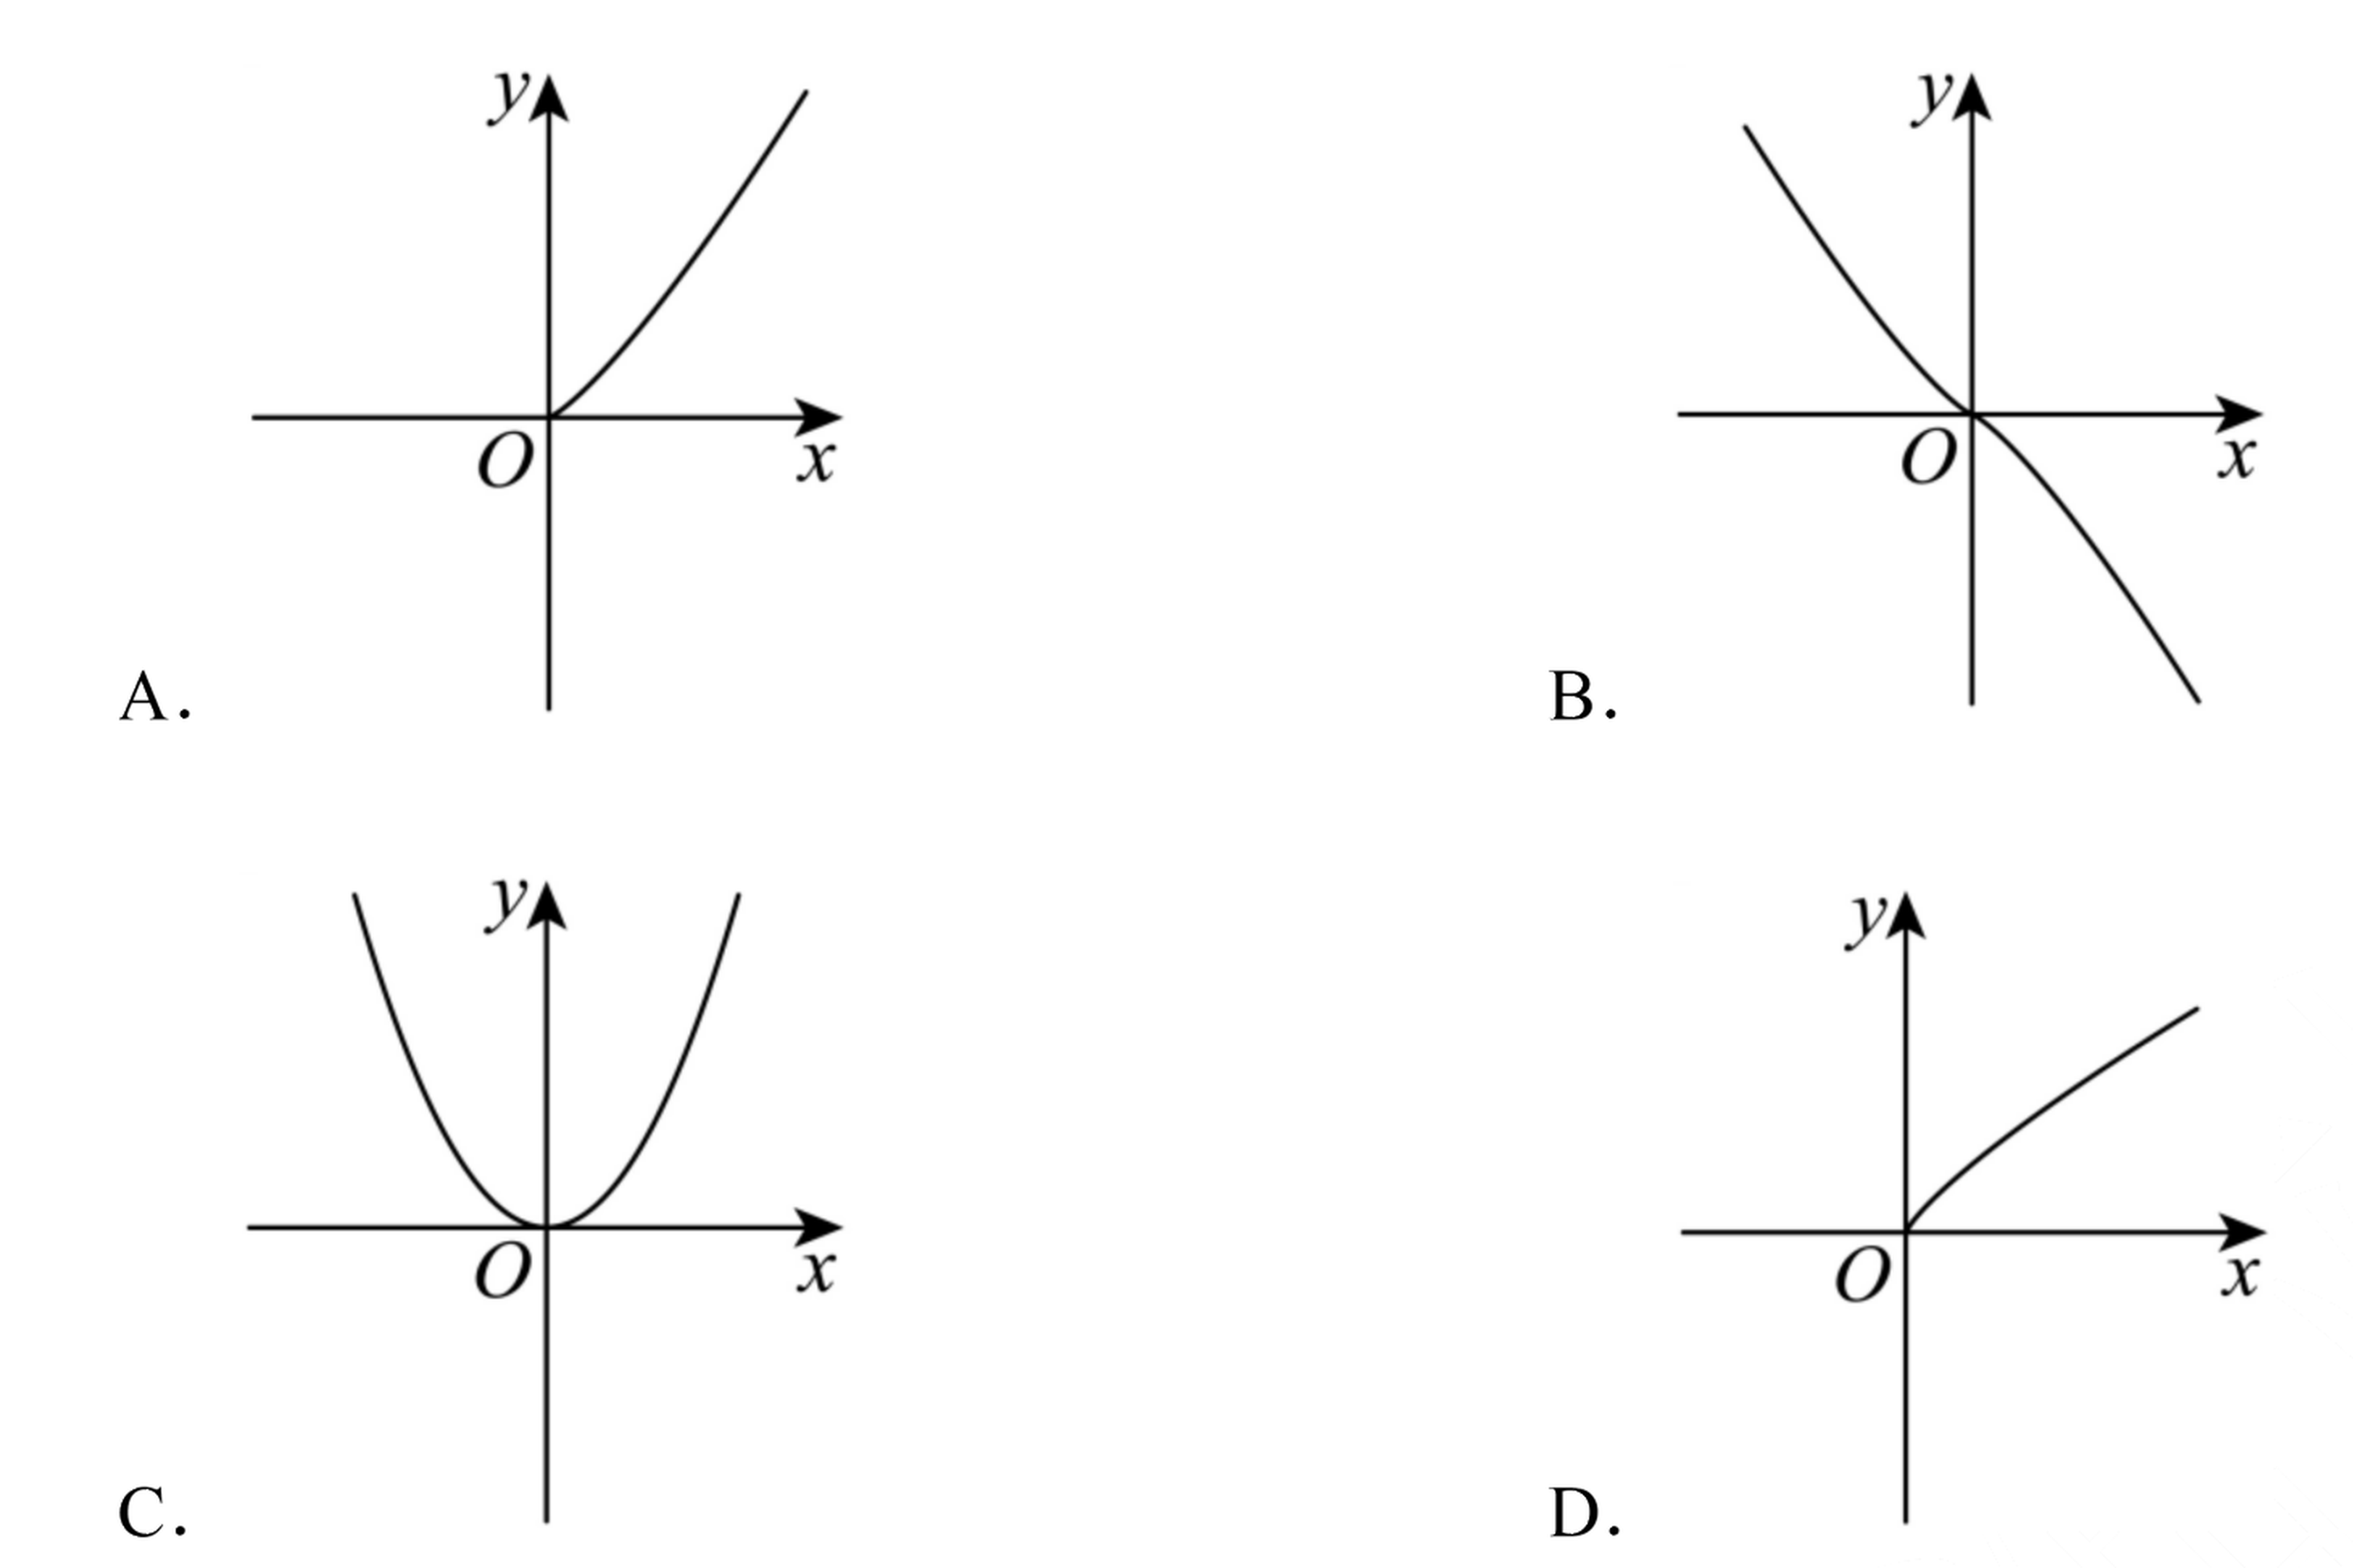
\includegraphics[width=0.80\textwidth]{figures/gao136_q13.png}
\end{center}

\ifanswer
\solbegin
\step{由 $y=x^{\frac54}=\sqrt[4]{x^5}$，函数的定义域为 $[0,+\infty)$，排除 BC，}% 原卷"排除 BC"连写，照录
\step{因为 $\dfrac54>1$，所以函数 $y=x^{\frac54}$ 的图象呈现下凸的趋势，排除 D. 故选 $A$.}
\solend
\fi

\item 下列不等式① $a+\dfrac1a\geqslant2$；② $a^2+4\geqslant4a$；③ $\left\lvert\dfrac ba+\dfrac ab\right\rvert\geqslant2$；④ $\dfrac{2a^2b^2}{a^2+b^2}\leqslant ab$；其中恒成立的是\mbox{（\quad）}

\keepwithprev
A. ①④\qquad B. ③④\qquad C. ②③\qquad D. ①②

\ifanswer
\ans{$C$}
\fi

\item 函数 $y=a^x+b-1(a>0,a\neq1)$ 单调递增且图象不经过第四象限，则 $a,b$ 满足的条件为\mbox{（\quad）}

\keepwithprev
A. $a>1,b\leqslant1$\qquad B. $a>1,b\geqslant0$\qquad C. $0<a<1,b\leqslant1$\qquad D. $0<a<1,b\geqslant1$

\ifanswer
\solbegin
\step{因为函数 $y=a^x+b-1$ 单调递增，所以 $a>1$，}
\step{图象不经过第四象限，则 $x=0$ 时，$y=b\geqslant0$，所以 $a>1,b\geqslant0$，故选 $B$.}
\solend
\fi

\item 设关于 $x$ 的不等式 $\dfrac{ax-1}{x^2-a}<0$ 的解集为 $S$，且 $3\in S$，$4\notin S$，则实数 $a$ 的取值范围为\mbox{（\quad）}

\keepwithprev
A. $(-\infty,-\sqrt3)\cup\left(\dfrac13,\sqrt3\right)$\qquad B. $\left(-\infty,\dfrac14\right)\cup(16,+\infty)$

C. $\left[\dfrac14,\dfrac13\right)\cup(9,16]$\qquad D. 不能确定

\ifanswer
\solbegin
\step{若 $3\in S$，则 $\dfrac{3a-1}{9-a}<0$，解得 $a\in\left(-\infty,\dfrac13\right)\cup(9,+\infty)$，}
\step{若 $4\notin S$，则 $16-a=0$ 或 $\dfrac{4a-1}{16-a}\geqslant0$，解得 $a\in\left[\dfrac14,16\right]$，}
\step{故实数 $a$ 的取值范围为 $\left[\dfrac14,\dfrac13\right)\cup(9,16]$，故选 $C$.}
\solend
\fi

\end{enumerate}

\bigsec{三、解答题}

\begin{enumerate}
\setcounter{enumi}{16}

\item 计算：(1) 计算 $\dfrac{\lg8+\lg125-\lg2-\lg5}{\lg\sqrt{10}\cdot\lg0.1}$；(2) 若 $a^{2x}=2(a>0)$，求 $\dfrac{a^{3x}+a^{-3x}}{a^x+a^{-x}}$.

\ifanswer
\solbegin
\step{(1) 原式 $=\dfrac{2-1}{\frac12\cdot(-1)}=-2$；(2) 原式 $=a^{2x}-1+a^{-2x}=2-1+\dfrac12=\dfrac32$.}
\solend
\fi

\item 不等式 $\dfrac{x-1}{x+1}\geqslant0$ 的解集为 $A$，不等式 $(x-a-1)(2a-x)>0(a<1)$ 的解集为 $B$.

(1) 求集合 $A$；

(2) 若 $B\subseteq A$，求实数 $a$ 的取值范围.

\ifanswer
\solbegin
\step{(1) $A=(-\infty,-1)\cup[1,+\infty)$.}
\step{(2) 由 $(x-a-1)(2a-x)>0(a<1)$，得 $(x-a-1)(x-2a)<0(a<1)$，}
\step{因为 $a<1$，所以 $a+1>2a$，所以 $B=(2a,a+1)$，}
\step{因为 $B\subseteq A$，所以 $2a\geqslant1$ 或 $a+1\leqslant-1$，即 $a\geqslant\dfrac12$ 或 $a\leqslant-2$，}
\step{而 $a<1$，所以实数 $a$ 的取值范围 $(-\infty,-2]\cup\left[\dfrac12,1\right)$.}% 原卷"取值范围"后脱"是／为"，照录
\solend
\fi

\item 已知幂函数 $y=x^m(m\in\R)$ 经过点 $\left(4,\dfrac12\right)$.

(1) 求此幂函数的表达式和定义域；

(2) 已知点 $A(a+2,y_1)$，点 $B(3-2a,y_2)(a\in\R)$ 在此幂函数的图像上，且满足 $y_1<y_2$，求实数 $a$ 的取值范围.

\ifanswer
\solbegin
\step{(1) 幂函数 $y=x^m(m\in\R)$ 经过点 $\left(4,\dfrac12\right)$，所以 $4^m=\dfrac12\Rightarrow m=-\dfrac12$，}
\step{所以 $f(x)=x^{-\frac12}$，定义域为 $(0,+\infty)$.}
\step{(2) 由于函数 $f(x)$ 在其定义域 $(0,+\infty)$ 上严格减，}
\step{由 $y_1<y_2$，得 $a+2>3-2a\geqslant0\Rightarrow a\in\left(\dfrac13,\dfrac32\right]$.}
\solend
\fi

% 第 20 题图取 05 页截图（0.42\textwidth、高约 6cm）。试排 \item 前加 7cm 守卫会多出
% 一张只有两行正文的稀疏页，且三版不加守卫时图均与题干、【解析】同页，故不另加守卫
\item 某医药研究所开发一种抗甲流新药，如果成年人按规定的剂量服用，据监测：服药后每毫升血液中的含药量 $y$（微克）与时间 $t$（小时）之间近似满足如图所示的曲线.

(1) 结合图，求 $k$ 与 $a$ 的值；

(2) 写出服药后 $y$ 与 $t$ 之间的函数关系式 $y=f(t)$；

(3) 据进一步测定：每毫升血液中含药量不少于 $0.5$ 微克时治疗疾病有效，求服药一次治疗有效的时间范围？

\begin{center}
% 图取原卷 05 页截图去粉色水印、去色，3x LANCZOS 放大
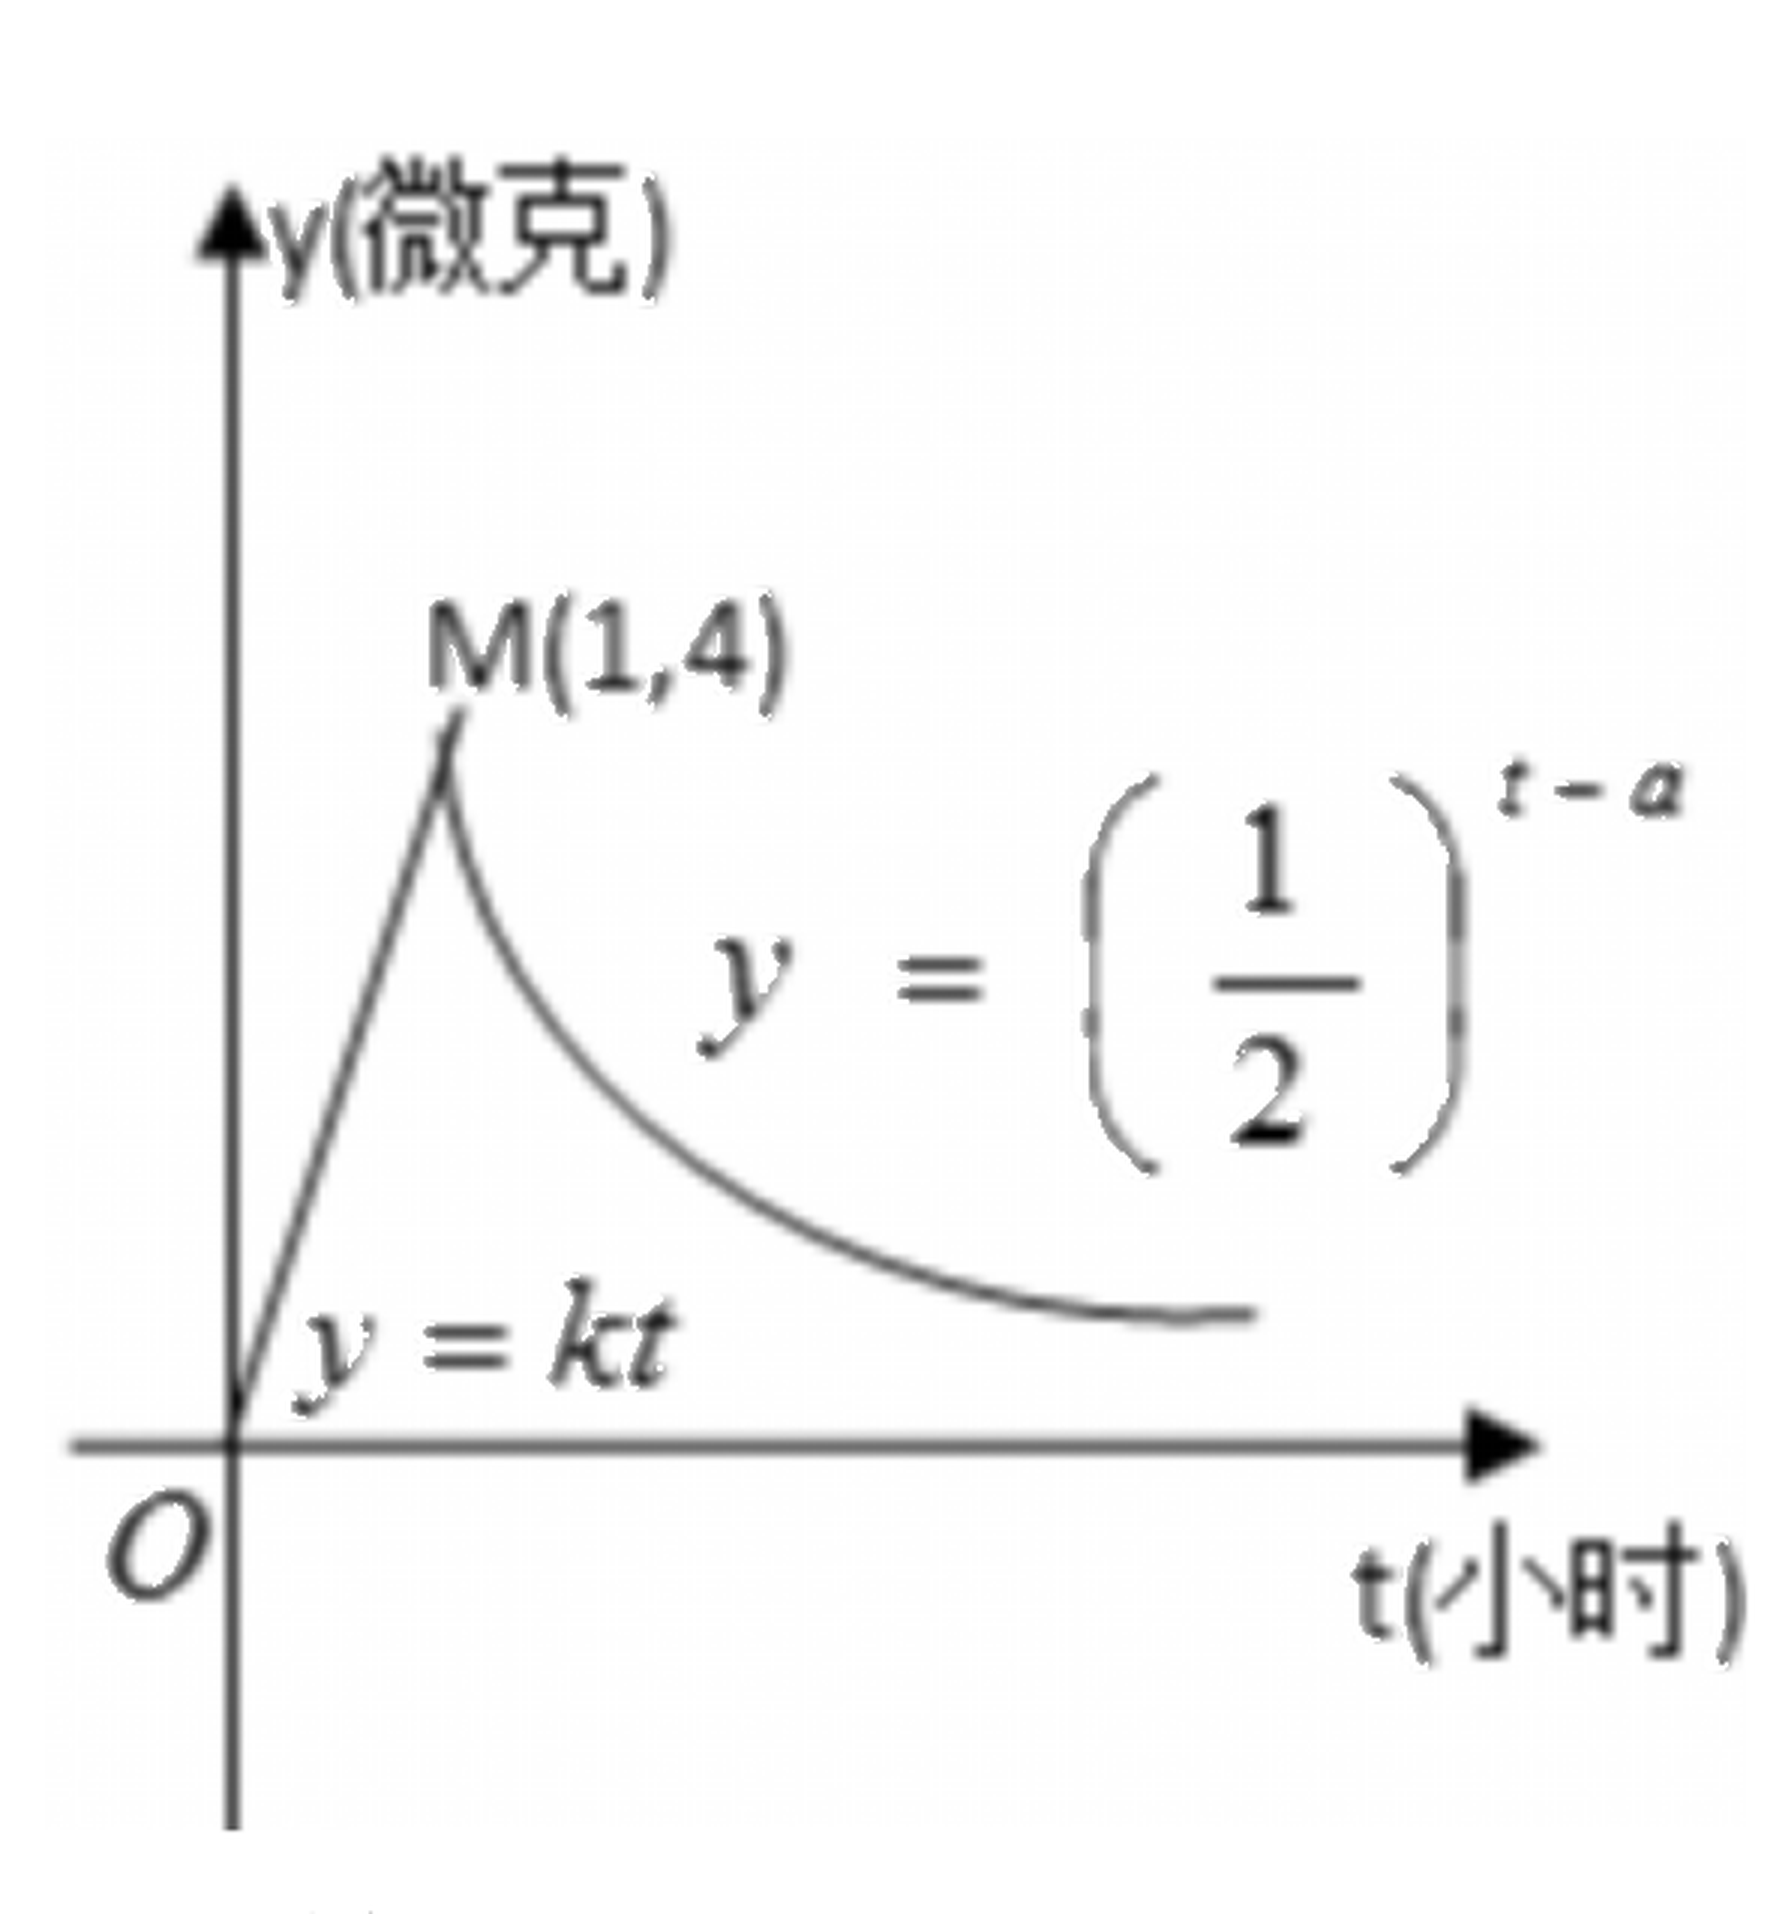
\includegraphics[width=0.42\textwidth]{figures/gao136_q20.png}
\end{center}

\ifanswer
\solbegin
\step{(1) 当 $0\leqslant t\leqslant1$ 时，函数图象是一条线段，由于过原点与点 $(1,4)$，所以 $k=4$，}
\step{其解析式为 $y=4t$，$0\leqslant t\leqslant1$；}
\step{当 $t\geqslant1$ 时，函数的解析式为 $y=\left(\dfrac12\right)^{t-a}$，}
\step{此时 $M(1,4)$ 在曲线上，将此点的坐标代入函数解析式得 $4=\left(\dfrac12\right)^{1-a}$，}
\step{解得 $a=3$；}
\step{(2) 由 (1) 得 $f(t)=\begin{cases}4t,0\leqslant t\leqslant1\\\left(\frac12\right)^{t-3},t>1\end{cases}$；}
\step{(3) 由 (2) 得，令 $f(t)\geqslant0.5$，即 $\begin{cases}4t\geqslant0.5,0\leqslant t\leqslant1\\\left(\frac12\right)^{t-3}\geqslant0.5,t>1\end{cases}$，所以 $\dfrac18\leqslant t\leqslant4$.}
\solend
\fi

\item 已知关于 $x$ 的不等式 $(kx-k^2-4)(x-4)>0$，其中 $k\in\R$.

(1) 当 $k=-1$，求不等式的解集 $A$；

(2) 当 $k$ 变化时，试求不等式的解集 $A$；

(3) 对于不等式解集 $A$，满足 $A\cap\Z=B$. 试探究集合 $B$ 能否为有限集，若能，求出使得集合 $B$ 中元素最少的 $k$ 的所有取值，并用列举法表示此时的集合 $B$，若不能，说明理由；

\ifanswer
\solbegin
\step{(1) 当 $k=-1$ 时，原不等式可化为 $(x+5)(x-4)<0$，}
\step{解得 $-5<x<4$，故不等式的解集为 $\{x\mid -5<x<4\}$；}
\step{(2) 当 $k=0$ 时，解集为 $\{x\mid x<4\}$，}
\step{当 $k>0$ 时，$\dfrac{k^2+4}{k}=k+\dfrac4k\geqslant4$，解集为 $\{x\mid x<4\text{ 或 }x>\dfrac{k^2+4}{k}\}$；}
\step{当 $k<0$ 时，解集为 $\{x\mid \dfrac{k^2+4}{k}<x<4\}$，}
\step{综上，当 $k=0$ 时，$A=\{x\mid x<4\}$，}
\step{当 $k>0$ 时，$A=\{x\mid x<4\text{ 或 }x>\dfrac{k^2+4}{k}\}$；}
\step{当 $k<0$ 时，$A=\{x\mid \dfrac{k^2+4}{k}<x<4\}$，}
\step{(3) 由 (2) 得当 $k\geqslant0$ 时，$B$ 为无限集，当 $k<0$ 时，$B$ 为有限集，}
\step{此时，$\dfrac{k^2+4}{k}=k+\dfrac4k\leqslant-4$，当且仅当 $k=-2$ 时取等号，}
\step{所以 $k=-2$ 时，$B$ 中元素最少，此时 $A=\{x\mid -4<x<4\}$，}
\step{所以 $B=\{-3,-2,-1,0,1,2,3\}$.}
\solend
\fi

\end{enumerate}

% 第 22 题是"四、附加题"首题且带 9cm 图块，守卫须放在 \bigsec 之前连节标题一起量，
% 否则"四、附加题"会孤立在页末（B 类，照 高一26／40／59 成例）
\needvspace{11cm}
\bigsec{四、附加题}

\begin{enumerate}
\setcounter{enumi}{21}

% 第 22 题四幅抛物线/坐标图选项是一整块，守卫放在 \item 之前
\needvspace{9cm}
\item 函数 $f(x)=\left(\dfrac12\right)^{\lvert x+1\rvert}$ 的图象大致为\mbox{（\quad）}

\keepwithprev
\begin{center}
% 四幅抛物线/坐标图选项取原卷 07 页截图去粉色水印，按原卷 2x2 排布合并为一张
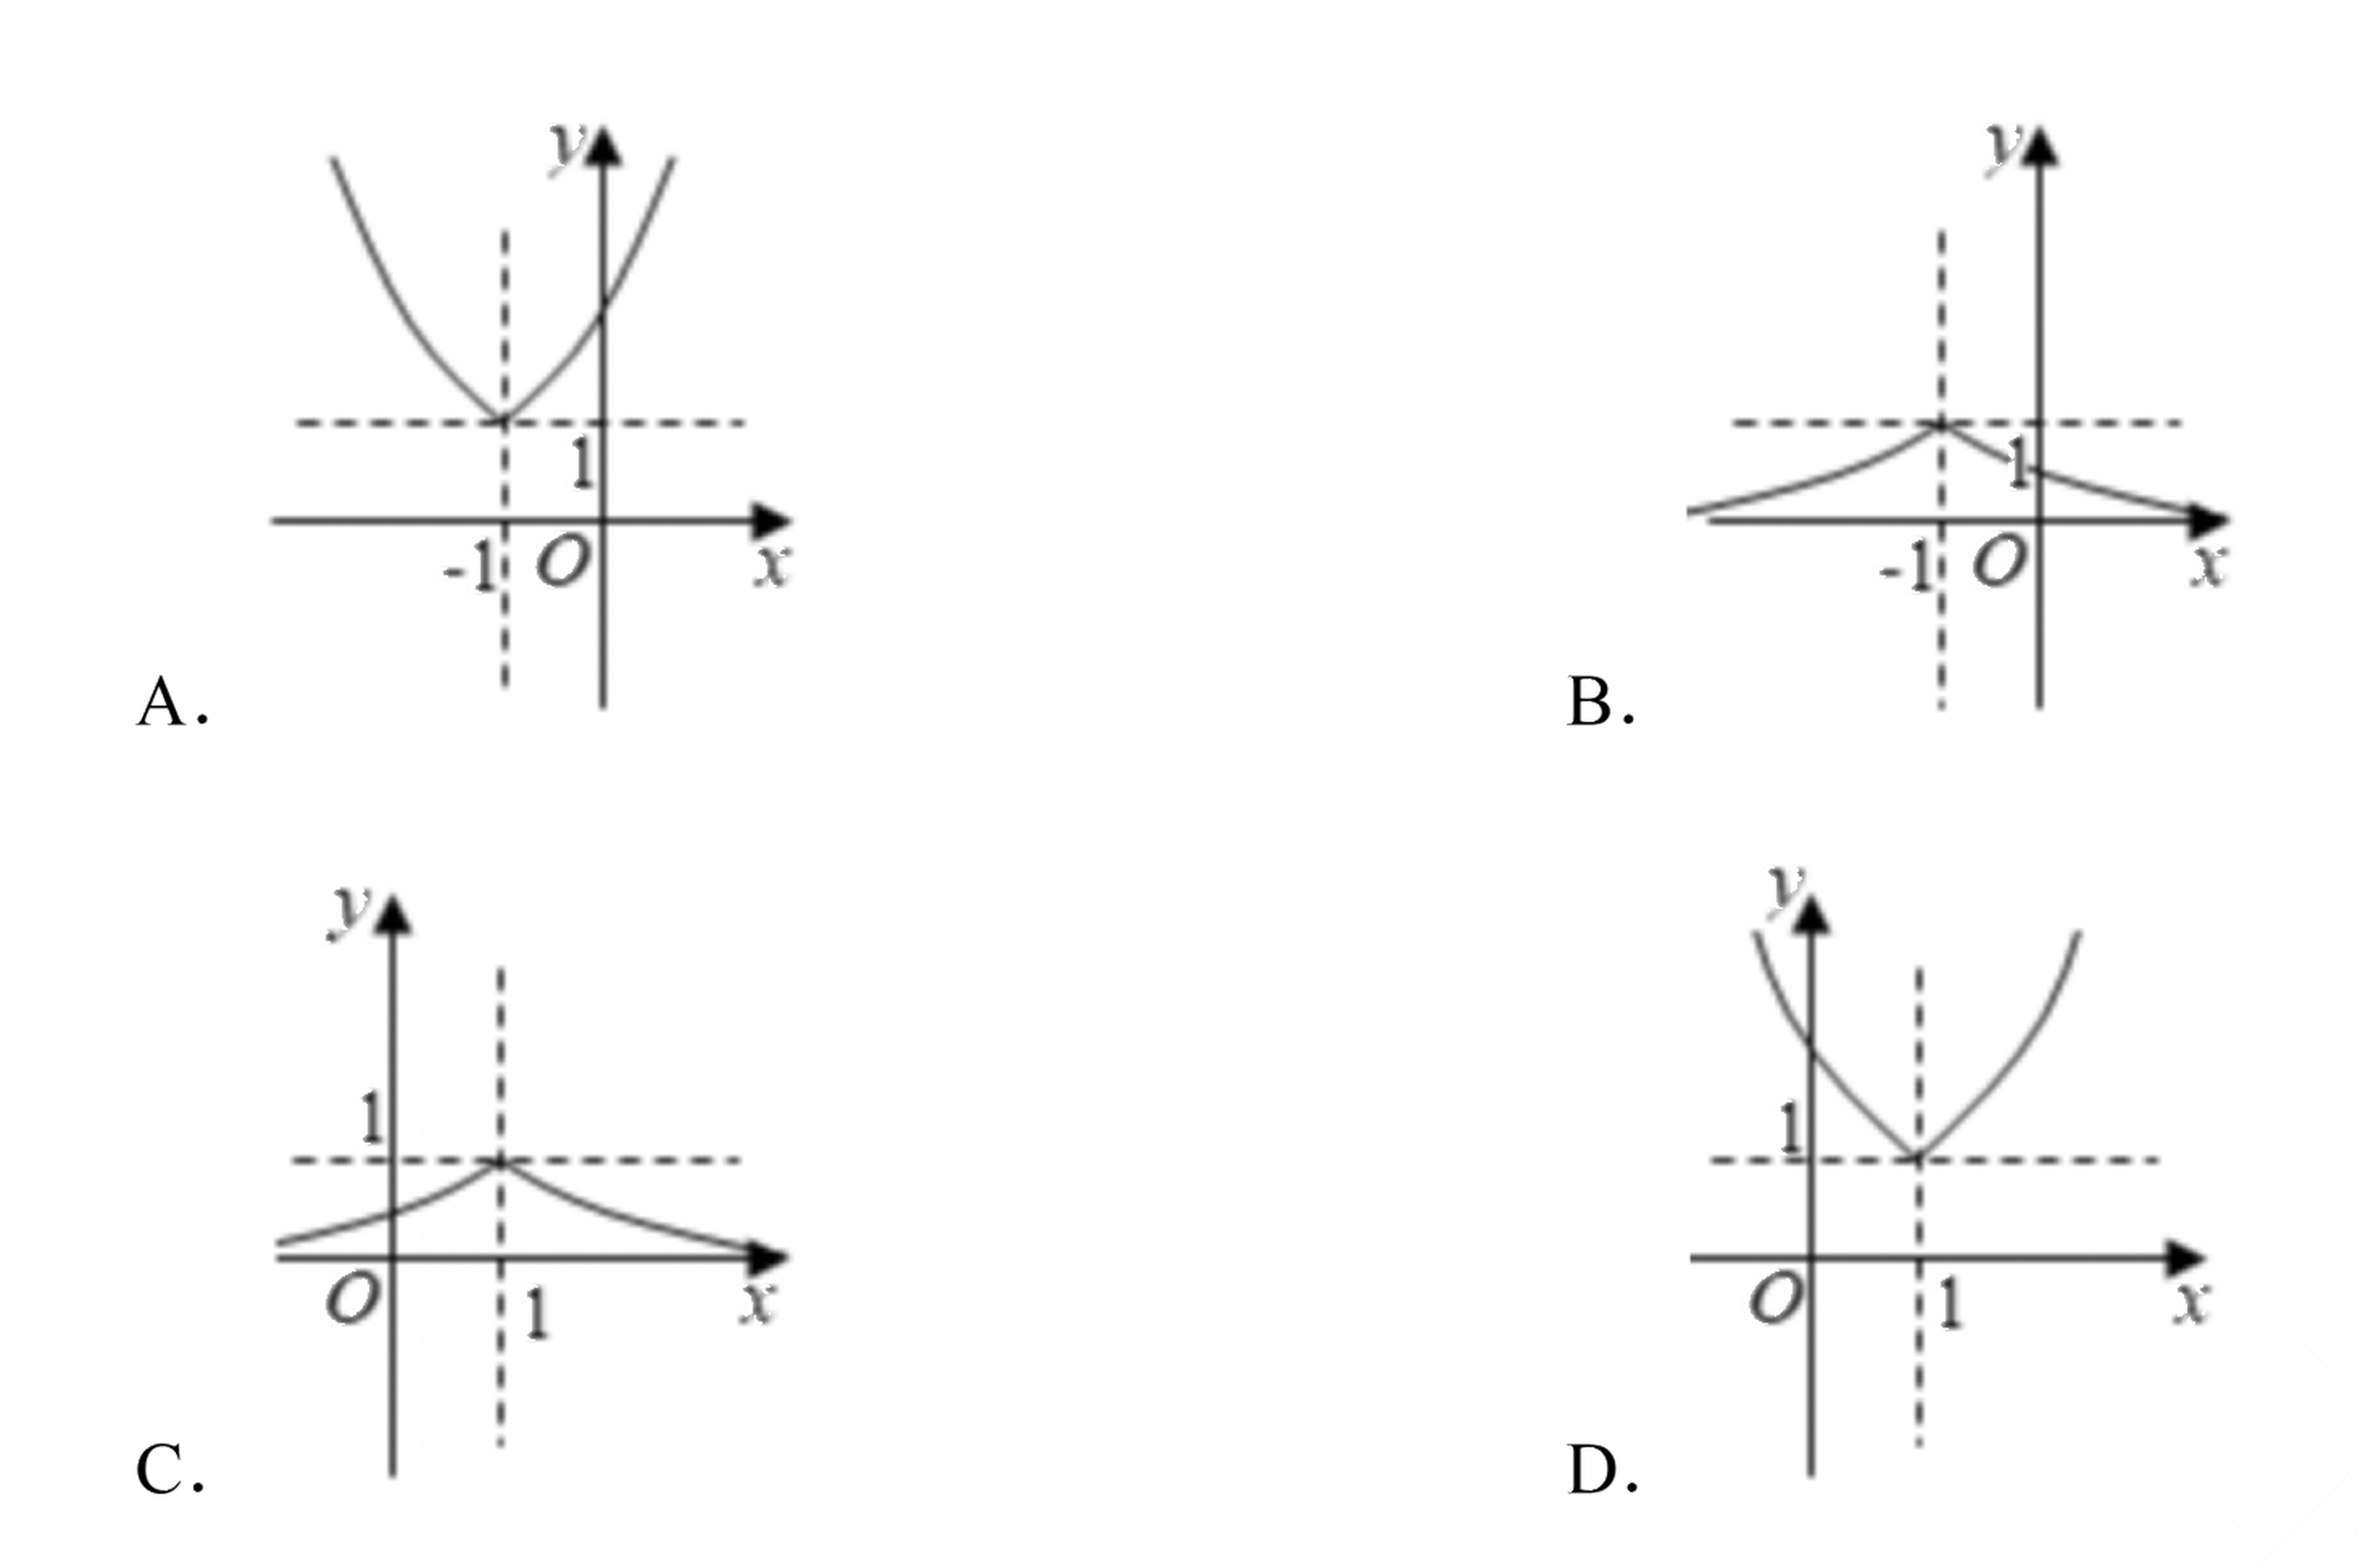
\includegraphics[width=0.80\textwidth]{figures/gao136_q22.png}
\end{center}

\ifanswer
\ans{$B$}
\fi

\end{enumerate}

\end{document}
"
%
% ① 原始材料：微信公众号"魔都数学加油站"文章，作者破晓，2026-11-15 18:04 发布；
% 连载"27学年高一136"，原文标题"27学年高一136——2026-2027年上海市三林中学高一上期中"；
% 原文链接：https://mp.weixin.qq.com/s/jaMzqMm6pDvcT0yM0d7eaQ。
% 正文为 7 张 PNG 页（01、04、06 为 4762x6735；02、03、05、07 为 2560x3620，
% 同一篇各页分辨率不同，逐页按各自分辨率裁图核对），题目下印有【答案】或【解析】，为讲评版。
% 题目、解析均据原图转录；卷面粉红色水印"魔都数学加油站"及公众号页脚未录入。
% 全卷 3 幅插图：第 13 题四幅坐标图选项（03 页）、第 20 题药物浓度折线/曲线图（05 页）、
% 第 22 题四幅抛物线/坐标图选项（07 页），均取原卷截图去粉色水印、去色、LANCZOS 放大，
% 四幅选项按原卷 2x2 排布合并为一张；图前按惯例加 \needvspace 守卫。
%
% 卷首标题：原卷印作"2026-2027 年三林中学高一上期中"（公众号标题中的"上海市"
% 卷面标题行没有，本稿照卷面），年份区间按全稿惯例排 en dash；原卷未印副标题，
% 本卷为期中卷、跨集合与常用逻辑用语／不等式／函数三章，按题目内容标为
% "集合与常用逻辑用语、不等式、函数"（与 125／126／128／129／131／132／133 同期中卷口径相同）：
% 集合与逻辑见 Q3、Q6、Q10、Q12、Q16、Q18、Q21，不等式见 Q5、Q7、Q8、Q9、Q14、Q15，
% 函数（幂函数、指数／对数、基本不等式应用）见 Q4、Q11、Q13、Q17、Q19、Q20、Q22。
%
% 题号体例：本卷共 20 题——一、填空题 3—12（10 题）、二、选择题 13—16（4 题）、
% 三、解答题 17—21（5 题）、四、附加题 22（1 题）。四节分别
% \setcounter{enumi}{2}／{12}／{16}／{21}。
%
% ② 与原卷的排版差异：
%   ① 原文从第 3 题起，本稿保留原题号；末节"四、附加题"另起 \bigsec，题号续到 22；
%   ② 原卷每题下直接印【答案】或【解析】，本稿按全稿惯例置于答案版；第 3、4、6 题只印
%      【答案】、无【解析】，提 \ans{}；第 14 题答案 C 印在题干括号内、无【解析】，按
%      高一53／高一108／高一132／高一133 成例括号留空、另提 \ans{$C$}；第 22 题答案 B
%      印在题干括号内、无【解析】，同例提 \ans{$B$}；第 13、15、16 题答案在解析末句
%      "故选 …"，括号内留空、不另提 \ans{}；其余各题印【解析】、无独立答案段；
%   ③ 原卷未印副标题，本稿按"知识模块"口径补出；
%   ④ 原卷填空横线按全稿惯例排为 \blankline[4.4em]；选择题括号排 \mbox{（\quad）}、
%      每个选项段前按惯例加 \keepwithprev（四幅图选项那一枚放在 \begin{center} 之前）；
%      解答题不留作答区、不加 \anspace（原卷为讲评版，与 129／131／132／133 同）；
%   ⑤ 原卷数集排斜体 $R$／$R^+$／$Z$，按全稿惯例改 \R／\R^+／\Z；空集记号 \varnothing；
%      绝对值排 \lvert…\rvert，集合描述竖线排 \mid；不等号按全稿惯例排 \leqslant／\geqslant；
%   ⑥ 子题标号 (1)(2)(3) 原卷用半角括号，照录；圈数字 ①②③④ 照录；第 12 题甲／乙／丙
%      三行与第 14 题四个编号不等式照录；
%   ⑦ 数学式内半角逗号照录（如 Q4"$a>0,a\neq1$"、Q6"$\{(-2,4),(1,1)\}$"、
%      Q7"$a=2+3=5,b=2\times3=6$"、Q11"$x_1,x_2$"、Q12"$m,n\in R^+$"、
%      Q15"$a>1,b\geq0$"、Q18"$B=(2a,a+1)$"、Q20"$4t,0\leq t\leq1$"、
%      Q21"$\{-3,-2,-1,0,1,2,3\}$"）；原卷行末西文句点照录，行中全角逗号照录；
%   ⑧ 三幅插图：第 13 题四幅坐标图选项合并裁为一张 \includegraphics（题前 \needvspace{9cm}）；
%      第 20 题折线/曲线图取 05 页截图（0.42\textwidth）；第 22 题四幅抛物线/坐标图选项合并
%      裁为一张（题前 \needvspace{9cm}）。第 13、22 题分别是"二、选择题""四、附加题"的首题
%      且带大图块，另在两处 \bigsec 之前各加 \needvspace{11cm} 连节标题一起量，避免节标题
%      孤立在页末（切页审计 B 类；照 高一26／40／59 成例）。第 20 题图不是节首题、三版试排
%      图均与题干同页，加 7cm 守卫反会多出一张只有两行正文的稀疏页，故不另加守卫；
%      三版切页审计均"合计异常：无"（试卷 4 页／紧凑 4 页／答案 6 页）；
%   ⑨ 跨页续印按题合并：Q16 题干在 03 页、括号与选项及【解析】在 04 页；Q19 题干在 04 页、
%      (2) 与【解析】在 05 页；Q20 (3)【解析】在 06 页；Q22 四幅图在 07 页；本稿按题连排；
%   ⑩ 题干中的中文弯引号按原卷照录，注释内一律 ASCII 引号；原卷"图像／图象"两种写法混用，
%      逐处照录（Q4、Q19 作"图像"，Q13、Q15、Q20、Q22 作"图象"）；
%   ⑪ 附加题节：原卷印"四、附加题"，本稿用 \bigsec{四、附加题} 另起一节、
%      \setcounter{enumi}{21}，顶层 1 个 \item（与 高一09／15／16／22／35／39／47／61 同口径）；
%      Q22 只印括号内答案、提 \ans{}，不计入 \step 账。
%
% 判别式字形：全卷仅第 9 题【解析】cases 块出现判别式"$\Delta=a^2-8a<0$"，原卷印
%   等腰、偏高的三角 $\Delta$，逐处放大核对并照录 \Delta；全卷未出现扁等边三角 \triangle。
%
% 子集符号：第 18 题 (2) 题干"$B\subseteq A$"与【解析】"$B\subseteq A$"两处原卷均印
%   带下划线 $\subseteq$，逐处放大核对、照录 \subseteq；全卷未出现单线 \subset。
%
% 原卷存疑照录（均照录未改，正文对应处另有 % 注）：
%   第 12 题乙行"$\dfrac{m+n}{mm}=\dfrac1{mn}$"前一分母印作 $mm$（后一处作 $mn$），照录；
%   第 12 题【解析】"$\geqslant\dfrac1{100}\left[a^2+1+2\sqrt{a^2}\right]$"保留 $\sqrt{a^2}$
%      未化简为 $a$，照录；
%   第 13 题【解析】"排除 BC"与"排除 D"连写选项字母，照录；
%   第 18 题 (2)【解析】末行"所以实数 $a$ 的取值范围 $(-\infty,-2]\cup[\frac12,1)$"
%      "取值范围"后脱"是／为"字，照录；
%   第 21 题 (3) 题干"求出使得集合 $B$ 中元素最少的 $k$ 的所有取值"而【解析】只给出
%      $k=-2$ 一处，措辞照录。
%
% 行数复核：逐题数 \step 条数，合计 51 条（Q3：0；Q4：0；Q5：2；Q6：0；Q7：2；Q8：1；
% Q9：1；Q10：4；Q11：1；Q12：4；Q13：2；Q14：0；Q15：2；Q16：3；Q17：1；Q18：5；
% Q19：4；Q20：7；Q21：12；Q22：0），与原卷印刷行逐题相等（cases 块作一个印刷行计）。
% 第 3、4、6、14、22 题只印【答案】、提 \ans{}，不计入 \step 账；第 13、15、16 题答案在
% 解析末句，括号内留空、不另提 \ans{}。
%
\documentclass[a4paper,11pt]{article}
\usepackage{common}

\begin{document}

\examtitlest[3]{2026--2027 年三林中学高一上期中}{集合与常用逻辑用语、不等式、函数}

\bigsec{一、填空题}

\begin{enumerate}
\setcounter{enumi}{2}

\item 用反证法证明命题“若 $x+y\neq5$，则 $x\neq2$ 或 $y\neq3$”为真命题时，第一个步骤是\blankline[4.4em].

\ifanswer
\ans{假设 $x=2$ 且 $y=3$}
\fi

\item 函数 $y=a^{x-1}+1(a>0,a\neq1)$ 的图像恒过定点 $A$，则点的坐标是\blankline[4.4em].

\ifanswer
\ans{$(1,2)$}
\fi

\item 已知 $x>1$，则 $x+\dfrac4{x-1}$ 的最小值是\blankline[4.4em].

\ifanswer
\solbegin
\step{由 $x>1$，得 $x-1>0$，则 $x+\dfrac4{x-1}=x-1+\dfrac4{x-1}+1\geqslant2\sqrt{(x-1)\cdot\dfrac4{x-1}}+1=5$，}
\step{当且仅当 $x-1=\dfrac4{x-1}$ 即 $x=3$ 时取等号，取得最小值 $5$.}
\solend
\fi

\item 已知集合 $A=\{(x,y)\mid y=x^2\}$，集合 $B=\{(x,y)\mid y=2-x\}$，求 $A\cap B=$\blankline[4.4em].

\ifanswer
\ans{$\{(-2,4),(1,1)\}$}
\fi

\item 已知一元二次不等式 $x^2-ax+b<0$ 的解集为 $(2,3)$，则不等式 $bx^2-ax+1>0$ 的解集是\blankline[4.4em].

\ifanswer
\solbegin
\step{$a=2+3=5,b=2\times3=6$，则 $bx^2-ax+1>0$ 即 $6x^2-5x+1>0$，}
\step{即 $(3x-1)(2x-1)>0$，解集为 $\left(-\infty,\dfrac13\right)\cup\left(\dfrac12,+\infty\right)$.}
\solend
\fi

\item 不等式 $(x+2)^3<(5-2x)^3$ 的解集为\blankline[4.4em].

\ifanswer
\solbegin
\step{由 $(x+2)^3<(5-2x)^3$ 得 $x+2<5-2x$，故解集为 $(-\infty,1)$.}
\solend
\fi

\item 若关于 $x$ 的不等式 $ax^2-ax+2>0$ 的解集为 $\R$，则实数 $a$ 的取值范围是\blankline[4.4em].

\ifanswer
\solbegin
\step{由题意得 $a=0$ 或 $\begin{cases}a>0\\\Delta=a^2-8a<0\end{cases}$，所以 $0\leqslant a<8$.}% 判别式原卷印高三角 $\Delta$，照录
\solend
\fi

\item 已知关于 $x$ 的不等式 $\lvert x+3\rvert+\lvert x-a\rvert\geqslant5$ 恒成立，则实数 $a$ 的取值范围为\blankline[4.4em].

\ifanswer
\solbegin
\step{因为 $\lvert x+3\rvert+\lvert x-a\rvert\geqslant\lvert x-a-x-3\rvert=\lvert 3+a\rvert$，}
\step{要使 $\lvert x+3\rvert+\lvert x-a\rvert\geqslant5$ 恒成立，则 $\lvert a+3\rvert\geqslant5$ 即可，}
\step{所以 $a+3\geqslant5$ 或 $a+3\leqslant-5$，解得 $a\geqslant2$ 或 $a\leqslant-8$，}
\step{即实数 $a$ 的取值范围是 $(-\infty,-8]\cup[2,+\infty)$.}
\solend
\fi

\item 若方程 $\lg^2 x-2\lg x-2=0$ 的两个解为 $x_1,x_2$，求 $\log_{x_1}x_2+\log_{x_2}x_1$ 的值为\blankline[4.4em].

\ifanswer
\solbegin
\step{$\log_{x_1}x_2+\log_{x_2}x_1=\dfrac{\lg x_2}{\lg x_1}+\dfrac{\lg x_1}{\lg x_2}=\dfrac{(\lg x_1+\lg x_2)^2-2\lg x_1\lg x_2}{\lg x_1\lg x_2}=-4$.}
\solend
\fi

\item 三个同学对问题“已知 $m,n\in \R^+$，且 $m+n=1$，求 $\dfrac1m+\dfrac1n$ 的最小值”提出各自的解题思路：

思路：

甲：$\dfrac1m+\dfrac1n=\dfrac{m+n}{m}+\dfrac{m+n}{n}=2+\dfrac nm+\dfrac mn$，可用基本不等式求解；

乙：$\dfrac1m+\dfrac1n=\dfrac{m+n}{mm}=\dfrac1{mn}=\dfrac1{m(1-m)}$，可用二次函数配方法求解；% 原卷前一分母印作 $mm$，照录

丙：$\dfrac1m+\dfrac1n=\left(\dfrac1m+\dfrac1n\right)(m+n)=2+\dfrac nm+\dfrac mn$，可用基本不等式求解；参考上述解题思路，

可求得当 $x=$\blankline[4.4em]时，$y=\dfrac{a^2}{x^2}+\dfrac1{100-x^2}$（$0<x<10$，$a>0$）有最小值.

\ifanswer
\solbegin
\step{$y=\dfrac{a^2}{x^2}+\dfrac1{100-x^2}=\left(\dfrac{a^2}{x^2}+\dfrac1{100-x^2}\right)[x^2+(100-x^2)]\times\dfrac1{100}$}
\step{$=\dfrac1{100}\left[a^2+1+\dfrac{x^2}{100-x^2}+\dfrac{a^2(100-x^2)}{x^2}\right]\geqslant\dfrac1{100}\left[a^2+1+2\sqrt{a^2}\right]$}% 原卷保留 $\sqrt{a^2}$ 未化简，照录
\step{当且仅当 $\dfrac{x^2}{100-x^2}=\dfrac{a^2(100-x^2)}{x^2}$，即 $x=\sqrt{\dfrac{100a}{a+1}}$ 时，}
\step{$y=\dfrac{a^2}{x^2}+\dfrac1{100-x^2}(0<x<10,a>0)$ 有最小值.}
\solend
\fi

\end{enumerate}

% 第 13 题是"二、选择题"首题且带 9cm 图块，守卫须放在 \bigsec 之前连节标题一起量，
% 否则"二、选择题"会孤立在页末（B 类，照 高一26／40／59 成例）
\needvspace{11cm}
\bigsec{二、选择题}

\begin{enumerate}
\setcounter{enumi}{12}

% 第 13 题四幅坐标图选项是一整块，守卫放在 \item 之前
\needvspace{9cm}
\item 下列图象中，最符合函数 $y=x^{\frac54}$ 的图象的是\mbox{（\quad）}

\keepwithprev
\begin{center}
% 四幅坐标图选项取原卷 03 页截图去粉色水印，按原卷 2x2 排布合并为一张
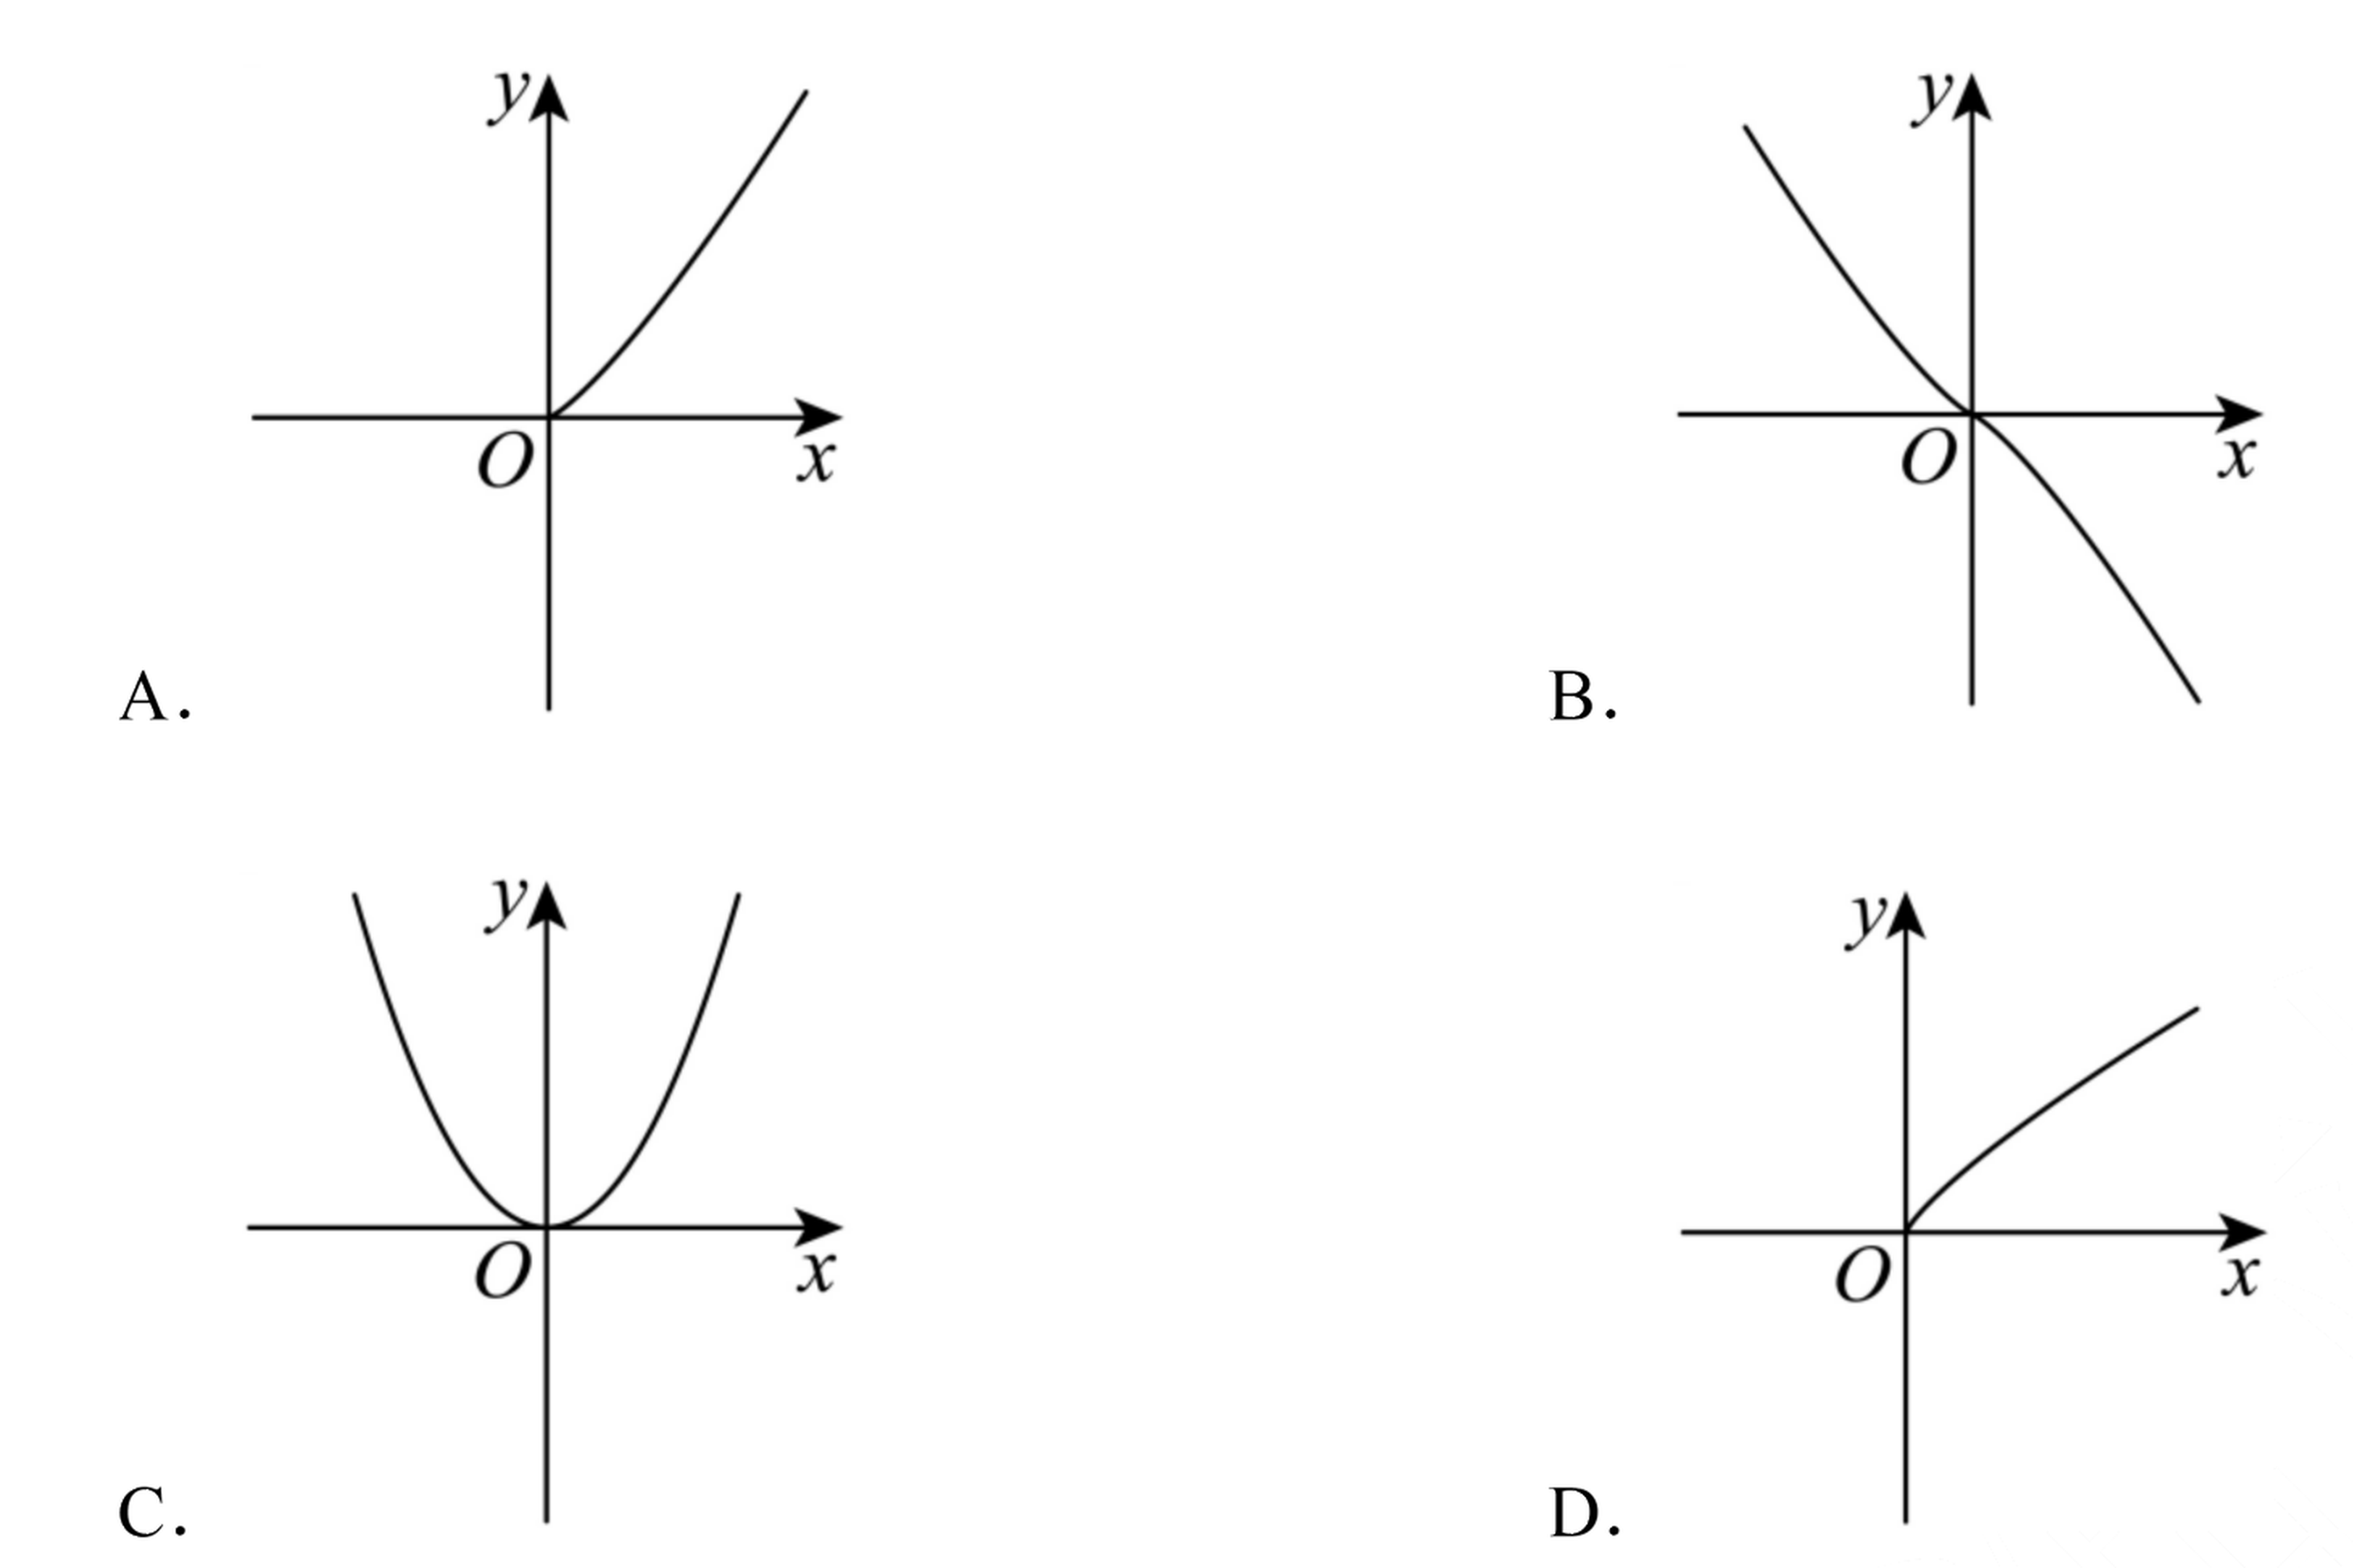
\includegraphics[width=0.80\textwidth]{figures/gao136_q13.png}
\end{center}

\ifanswer
\solbegin
\step{由 $y=x^{\frac54}=\sqrt[4]{x^5}$，函数的定义域为 $[0,+\infty)$，排除 BC，}% 原卷"排除 BC"连写，照录
\step{因为 $\dfrac54>1$，所以函数 $y=x^{\frac54}$ 的图象呈现下凸的趋势，排除 D. 故选 $A$.}
\solend
\fi

\item 下列不等式① $a+\dfrac1a\geqslant2$；② $a^2+4\geqslant4a$；③ $\left\lvert\dfrac ba+\dfrac ab\right\rvert\geqslant2$；④ $\dfrac{2a^2b^2}{a^2+b^2}\leqslant ab$；其中恒成立的是\mbox{（\quad）}

\keepwithprev
A. ①④\qquad B. ③④\qquad C. ②③\qquad D. ①②

\ifanswer
\ans{$C$}
\fi

\item 函数 $y=a^x+b-1(a>0,a\neq1)$ 单调递增且图象不经过第四象限，则 $a,b$ 满足的条件为\mbox{（\quad）}

\keepwithprev
A. $a>1,b\leqslant1$\qquad B. $a>1,b\geqslant0$\qquad C. $0<a<1,b\leqslant1$\qquad D. $0<a<1,b\geqslant1$

\ifanswer
\solbegin
\step{因为函数 $y=a^x+b-1$ 单调递增，所以 $a>1$，}
\step{图象不经过第四象限，则 $x=0$ 时，$y=b\geqslant0$，所以 $a>1,b\geqslant0$，故选 $B$.}
\solend
\fi

\item 设关于 $x$ 的不等式 $\dfrac{ax-1}{x^2-a}<0$ 的解集为 $S$，且 $3\in S$，$4\notin S$，则实数 $a$ 的取值范围为\mbox{（\quad）}

\keepwithprev
A. $(-\infty,-\sqrt3)\cup\left(\dfrac13,\sqrt3\right)$\qquad B. $\left(-\infty,\dfrac14\right)\cup(16,+\infty)$

C. $\left[\dfrac14,\dfrac13\right)\cup(9,16]$\qquad D. 不能确定

\ifanswer
\solbegin
\step{若 $3\in S$，则 $\dfrac{3a-1}{9-a}<0$，解得 $a\in\left(-\infty,\dfrac13\right)\cup(9,+\infty)$，}
\step{若 $4\notin S$，则 $16-a=0$ 或 $\dfrac{4a-1}{16-a}\geqslant0$，解得 $a\in\left[\dfrac14,16\right]$，}
\step{故实数 $a$ 的取值范围为 $\left[\dfrac14,\dfrac13\right)\cup(9,16]$，故选 $C$.}
\solend
\fi

\end{enumerate}

\bigsec{三、解答题}

\begin{enumerate}
\setcounter{enumi}{16}

\item 计算：(1) 计算 $\dfrac{\lg8+\lg125-\lg2-\lg5}{\lg\sqrt{10}\cdot\lg0.1}$；(2) 若 $a^{2x}=2(a>0)$，求 $\dfrac{a^{3x}+a^{-3x}}{a^x+a^{-x}}$.

\ifanswer
\solbegin
\step{(1) 原式 $=\dfrac{2-1}{\frac12\cdot(-1)}=-2$；(2) 原式 $=a^{2x}-1+a^{-2x}=2-1+\dfrac12=\dfrac32$.}
\solend
\fi

\item 不等式 $\dfrac{x-1}{x+1}\geqslant0$ 的解集为 $A$，不等式 $(x-a-1)(2a-x)>0(a<1)$ 的解集为 $B$.

(1) 求集合 $A$；

(2) 若 $B\subseteq A$，求实数 $a$ 的取值范围.

\ifanswer
\solbegin
\step{(1) $A=(-\infty,-1)\cup[1,+\infty)$.}
\step{(2) 由 $(x-a-1)(2a-x)>0(a<1)$，得 $(x-a-1)(x-2a)<0(a<1)$，}
\step{因为 $a<1$，所以 $a+1>2a$，所以 $B=(2a,a+1)$，}
\step{因为 $B\subseteq A$，所以 $2a\geqslant1$ 或 $a+1\leqslant-1$，即 $a\geqslant\dfrac12$ 或 $a\leqslant-2$，}
\step{而 $a<1$，所以实数 $a$ 的取值范围 $(-\infty,-2]\cup\left[\dfrac12,1\right)$.}% 原卷"取值范围"后脱"是／为"，照录
\solend
\fi

\item 已知幂函数 $y=x^m(m\in\R)$ 经过点 $\left(4,\dfrac12\right)$.

(1) 求此幂函数的表达式和定义域；

(2) 已知点 $A(a+2,y_1)$，点 $B(3-2a,y_2)(a\in\R)$ 在此幂函数的图像上，且满足 $y_1<y_2$，求实数 $a$ 的取值范围.

\ifanswer
\solbegin
\step{(1) 幂函数 $y=x^m(m\in\R)$ 经过点 $\left(4,\dfrac12\right)$，所以 $4^m=\dfrac12\Rightarrow m=-\dfrac12$，}
\step{所以 $f(x)=x^{-\frac12}$，定义域为 $(0,+\infty)$.}
\step{(2) 由于函数 $f(x)$ 在其定义域 $(0,+\infty)$ 上严格减，}
\step{由 $y_1<y_2$，得 $a+2>3-2a\geqslant0\Rightarrow a\in\left(\dfrac13,\dfrac32\right]$.}
\solend
\fi

% 第 20 题图取 05 页截图（0.42\textwidth、高约 6cm）。试排 \item 前加 7cm 守卫会多出
% 一张只有两行正文的稀疏页，且三版不加守卫时图均与题干、【解析】同页，故不另加守卫
\item 某医药研究所开发一种抗甲流新药，如果成年人按规定的剂量服用，据监测：服药后每毫升血液中的含药量 $y$（微克）与时间 $t$（小时）之间近似满足如图所示的曲线.

(1) 结合图，求 $k$ 与 $a$ 的值；

(2) 写出服药后 $y$ 与 $t$ 之间的函数关系式 $y=f(t)$；

(3) 据进一步测定：每毫升血液中含药量不少于 $0.5$ 微克时治疗疾病有效，求服药一次治疗有效的时间范围？

\begin{center}
% 图取原卷 05 页截图去粉色水印、去色，3x LANCZOS 放大
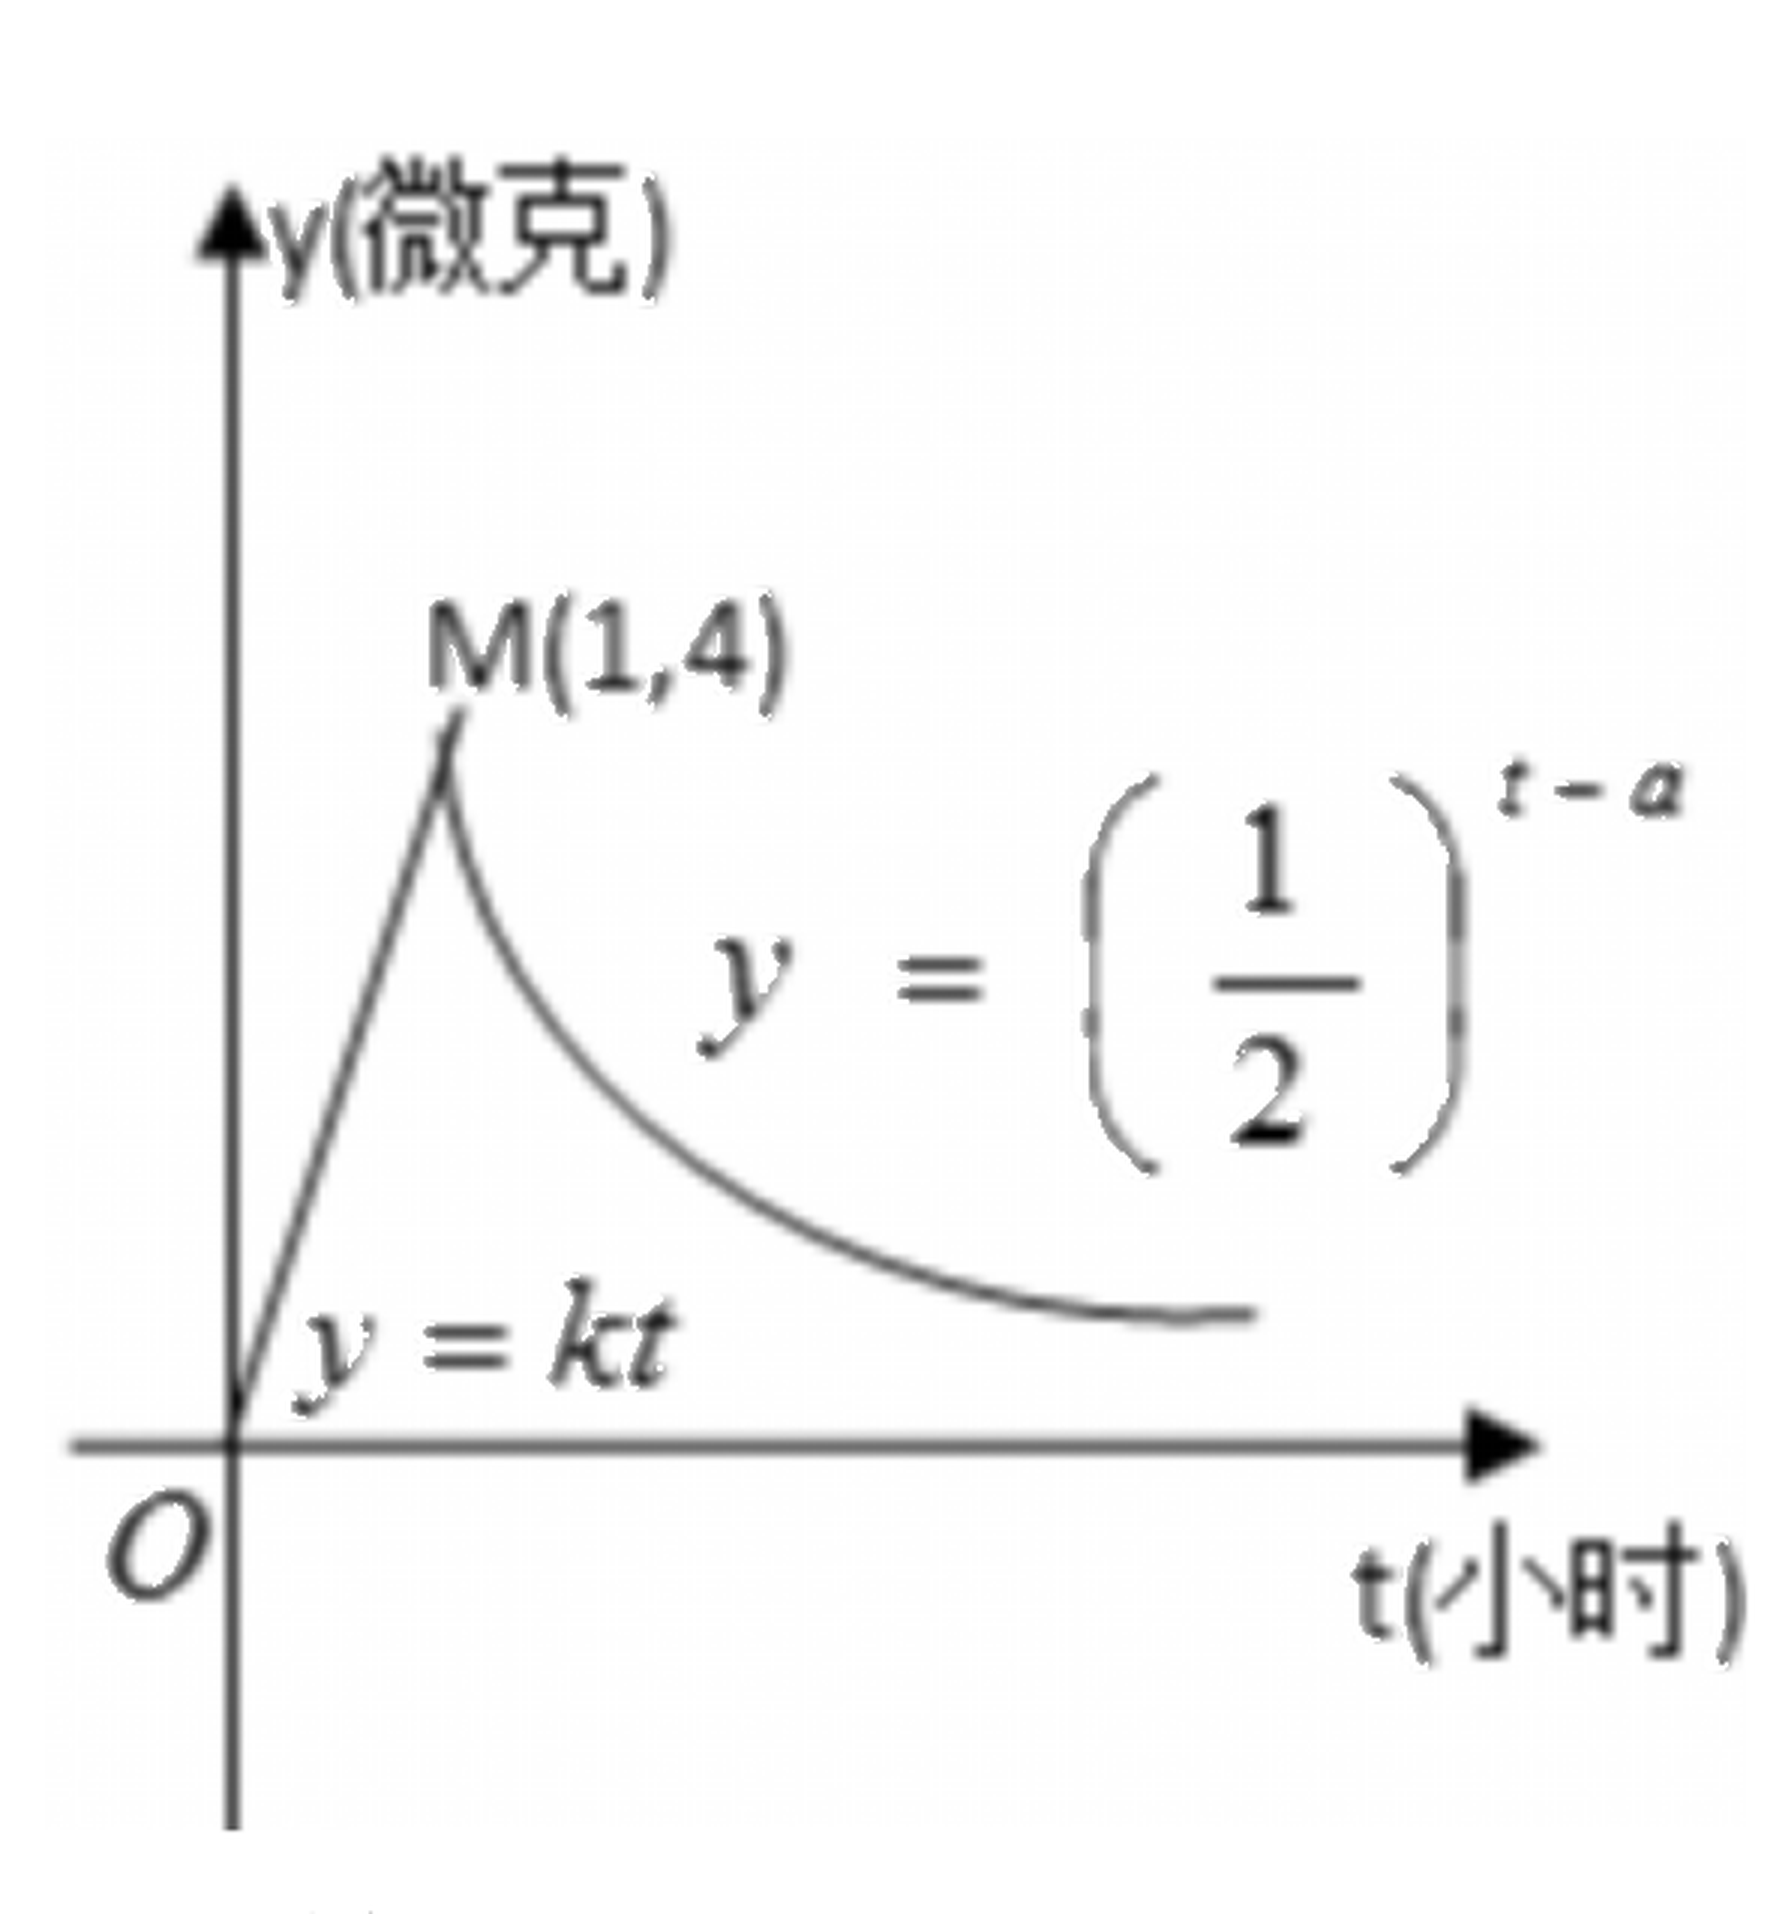
\includegraphics[width=0.42\textwidth]{figures/gao136_q20.png}
\end{center}

\ifanswer
\solbegin
\step{(1) 当 $0\leqslant t\leqslant1$ 时，函数图象是一条线段，由于过原点与点 $(1,4)$，所以 $k=4$，}
\step{其解析式为 $y=4t$，$0\leqslant t\leqslant1$；}
\step{当 $t\geqslant1$ 时，函数的解析式为 $y=\left(\dfrac12\right)^{t-a}$，}
\step{此时 $M(1,4)$ 在曲线上，将此点的坐标代入函数解析式得 $4=\left(\dfrac12\right)^{1-a}$，}
\step{解得 $a=3$；}
\step{(2) 由 (1) 得 $f(t)=\begin{cases}4t,0\leqslant t\leqslant1\\\left(\frac12\right)^{t-3},t>1\end{cases}$；}
\step{(3) 由 (2) 得，令 $f(t)\geqslant0.5$，即 $\begin{cases}4t\geqslant0.5,0\leqslant t\leqslant1\\\left(\frac12\right)^{t-3}\geqslant0.5,t>1\end{cases}$，所以 $\dfrac18\leqslant t\leqslant4$.}
\solend
\fi

\item 已知关于 $x$ 的不等式 $(kx-k^2-4)(x-4)>0$，其中 $k\in\R$.

(1) 当 $k=-1$，求不等式的解集 $A$；

(2) 当 $k$ 变化时，试求不等式的解集 $A$；

(3) 对于不等式解集 $A$，满足 $A\cap\Z=B$. 试探究集合 $B$ 能否为有限集，若能，求出使得集合 $B$ 中元素最少的 $k$ 的所有取值，并用列举法表示此时的集合 $B$，若不能，说明理由；

\ifanswer
\solbegin
\step{(1) 当 $k=-1$ 时，原不等式可化为 $(x+5)(x-4)<0$，}
\step{解得 $-5<x<4$，故不等式的解集为 $\{x\mid -5<x<4\}$；}
\step{(2) 当 $k=0$ 时，解集为 $\{x\mid x<4\}$，}
\step{当 $k>0$ 时，$\dfrac{k^2+4}{k}=k+\dfrac4k\geqslant4$，解集为 $\{x\mid x<4\text{ 或 }x>\dfrac{k^2+4}{k}\}$；}
\step{当 $k<0$ 时，解集为 $\{x\mid \dfrac{k^2+4}{k}<x<4\}$，}
\step{综上，当 $k=0$ 时，$A=\{x\mid x<4\}$，}
\step{当 $k>0$ 时，$A=\{x\mid x<4\text{ 或 }x>\dfrac{k^2+4}{k}\}$；}
\step{当 $k<0$ 时，$A=\{x\mid \dfrac{k^2+4}{k}<x<4\}$，}
\step{(3) 由 (2) 得当 $k\geqslant0$ 时，$B$ 为无限集，当 $k<0$ 时，$B$ 为有限集，}
\step{此时，$\dfrac{k^2+4}{k}=k+\dfrac4k\leqslant-4$，当且仅当 $k=-2$ 时取等号，}
\step{所以 $k=-2$ 时，$B$ 中元素最少，此时 $A=\{x\mid -4<x<4\}$，}
\step{所以 $B=\{-3,-2,-1,0,1,2,3\}$.}
\solend
\fi

\end{enumerate}

% 第 22 题是"四、附加题"首题且带 9cm 图块，守卫须放在 \bigsec 之前连节标题一起量，
% 否则"四、附加题"会孤立在页末（B 类，照 高一26／40／59 成例）
\needvspace{11cm}
\bigsec{四、附加题}

\begin{enumerate}
\setcounter{enumi}{21}

% 第 22 题四幅抛物线/坐标图选项是一整块，守卫放在 \item 之前
\needvspace{9cm}
\item 函数 $f(x)=\left(\dfrac12\right)^{\lvert x+1\rvert}$ 的图象大致为\mbox{（\quad）}

\keepwithprev
\begin{center}
% 四幅抛物线/坐标图选项取原卷 07 页截图去粉色水印，按原卷 2x2 排布合并为一张
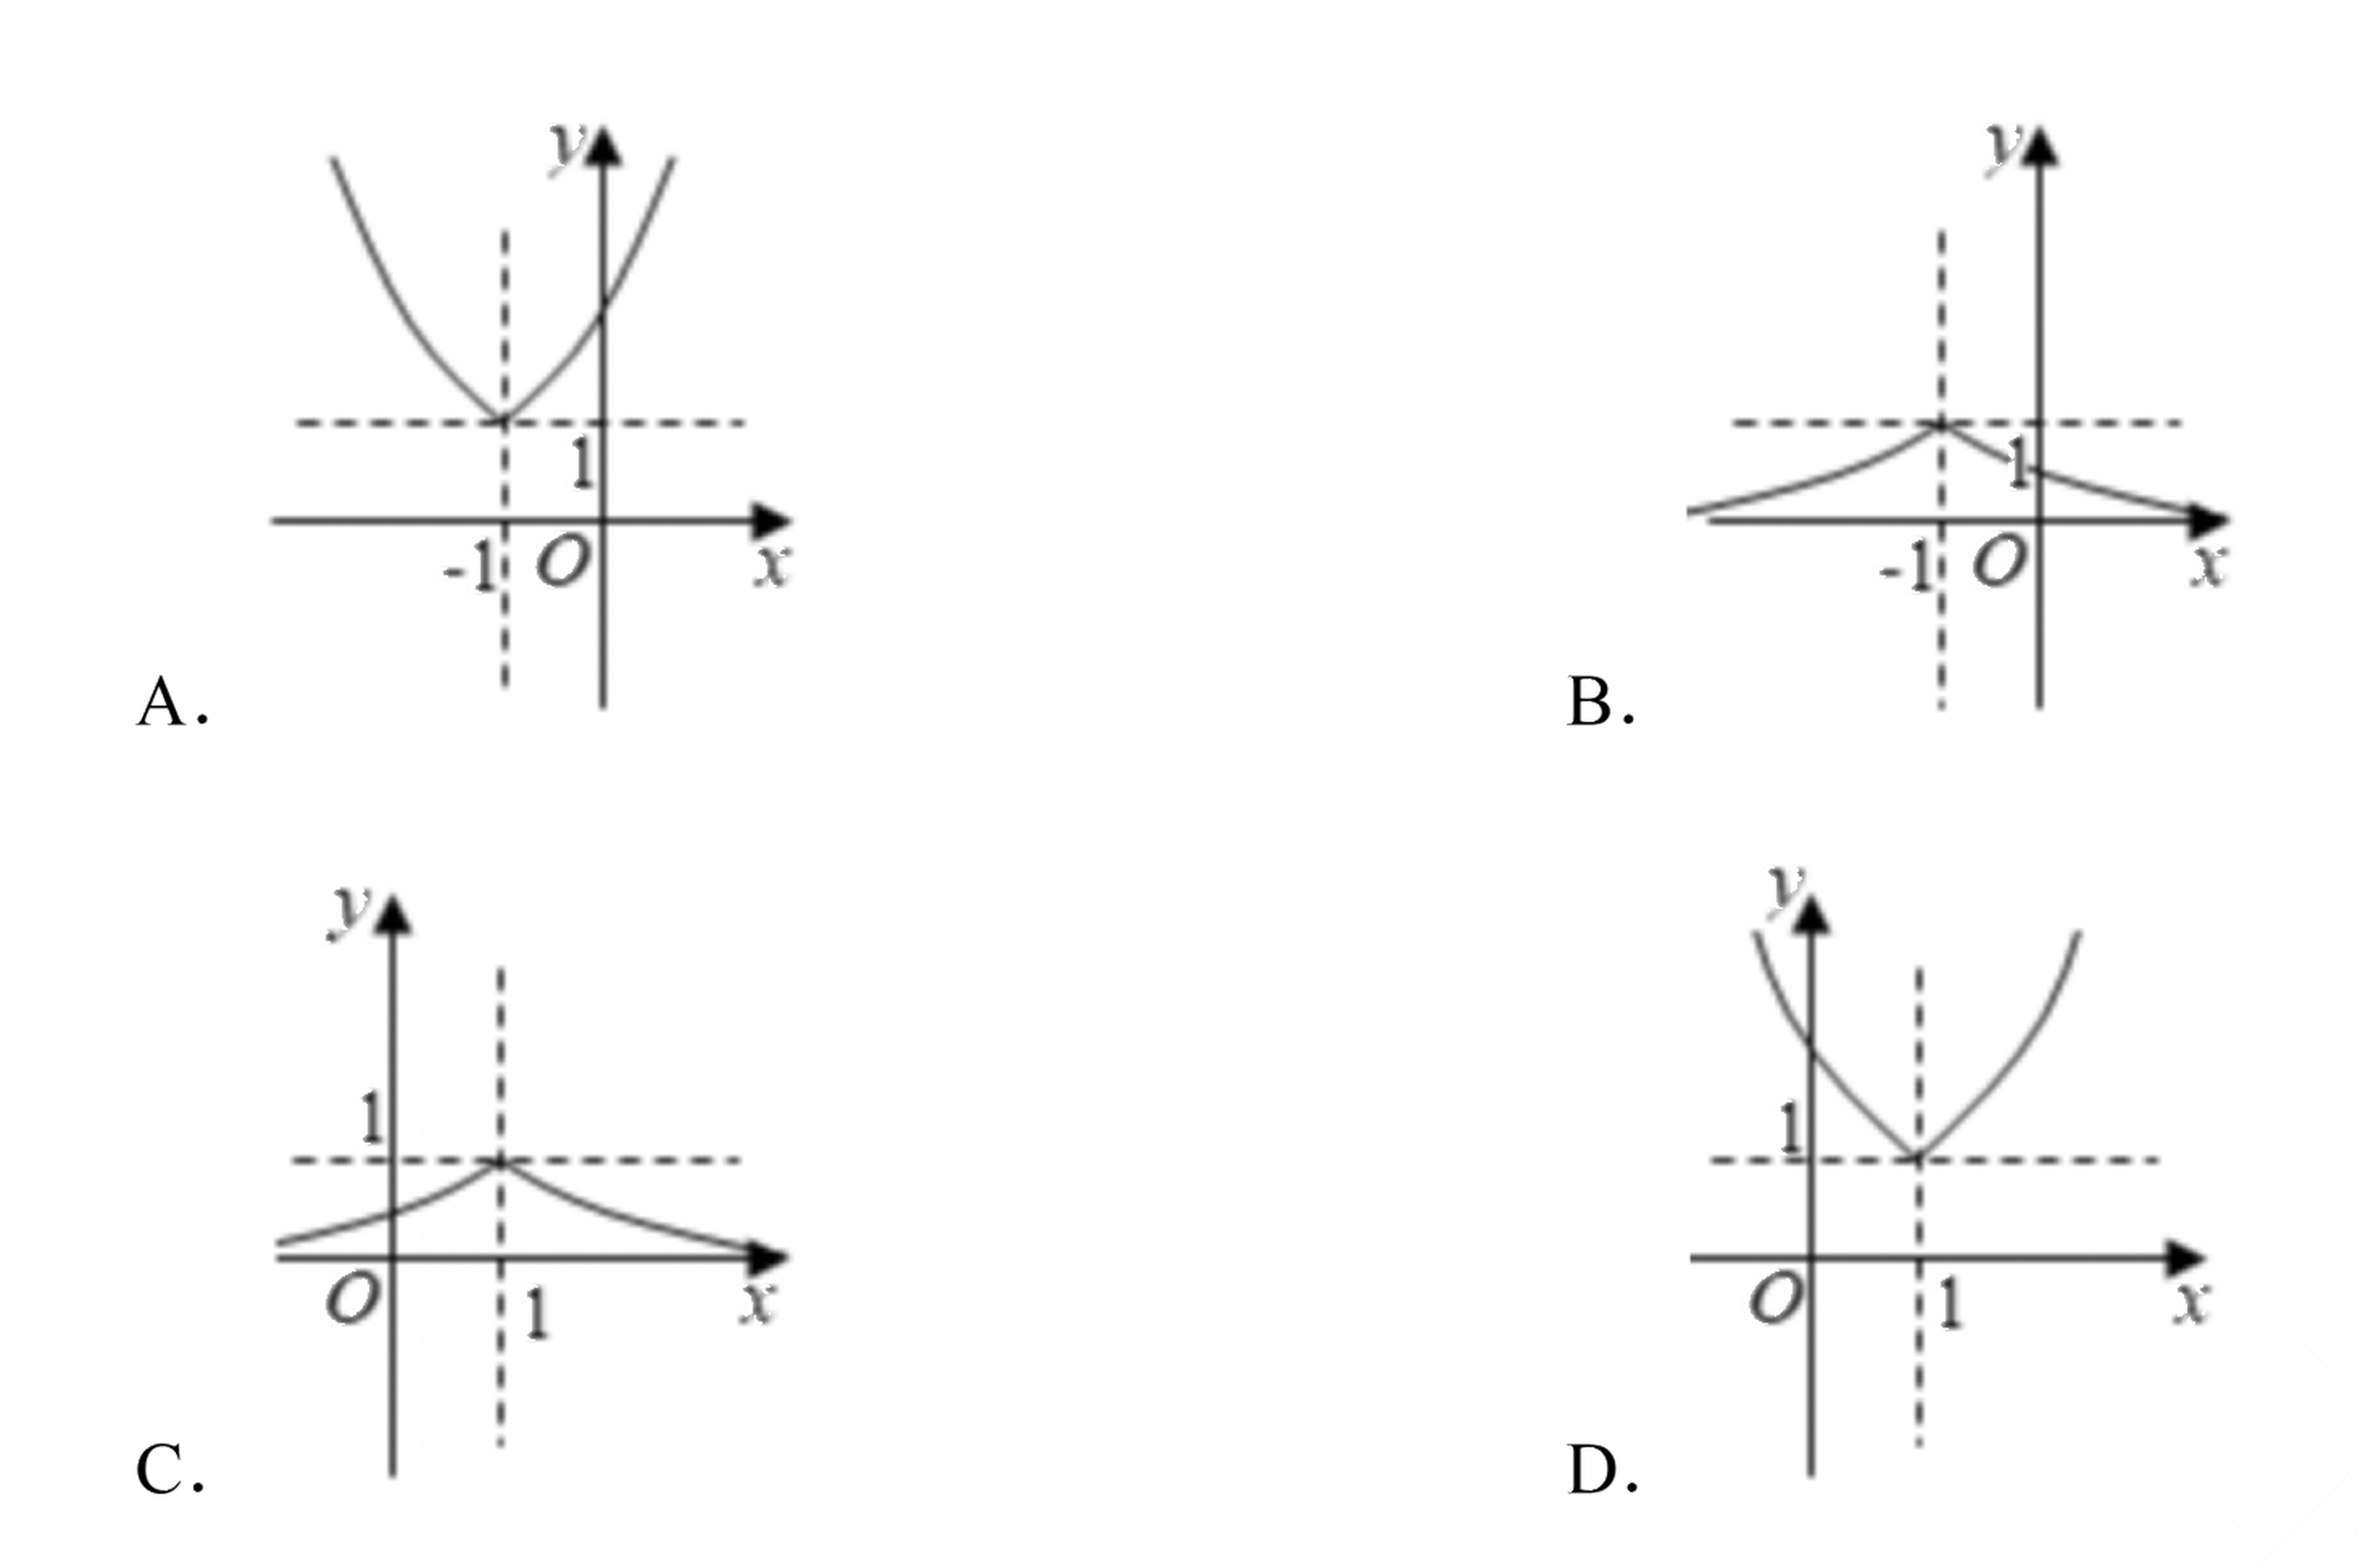
\includegraphics[width=0.80\textwidth]{figures/gao136_q22.png}
\end{center}

\ifanswer
\ans{$B$}
\fi

\end{enumerate}

\end{document}
"
% 紧凑版：xelatex "\def\iscompact{1}% 高一136_三林中学_期中.tex
%   —— 高一上数学"2026-2027 年三林中学高一上期中"（试卷版/答案版）
% 试卷版：xelatex 高一136_三林中学_期中.tex
% 答案版：xelatex "\def\isanswer{1}% 高一136_三林中学_期中.tex
%   —— 高一上数学"2026-2027 年三林中学高一上期中"（试卷版/答案版）
% 试卷版：xelatex 高一136_三林中学_期中.tex
% 答案版：xelatex "\def\isanswer{1}\input{高一136_三林中学_期中.tex}"
% 紧凑版：xelatex "\def\iscompact{1}\input{高一136_三林中学_期中.tex}"
%
% ① 原始材料：微信公众号"魔都数学加油站"文章，作者破晓，2026-11-15 18:04 发布；
% 连载"27学年高一136"，原文标题"27学年高一136——2026-2027年上海市三林中学高一上期中"；
% 原文链接：https://mp.weixin.qq.com/s/jaMzqMm6pDvcT0yM0d7eaQ。
% 正文为 7 张 PNG 页（01、04、06 为 4762x6735；02、03、05、07 为 2560x3620，
% 同一篇各页分辨率不同，逐页按各自分辨率裁图核对），题目下印有【答案】或【解析】，为讲评版。
% 题目、解析均据原图转录；卷面粉红色水印"魔都数学加油站"及公众号页脚未录入。
% 全卷 3 幅插图：第 13 题四幅坐标图选项（03 页）、第 20 题药物浓度折线/曲线图（05 页）、
% 第 22 题四幅抛物线/坐标图选项（07 页），均取原卷截图去粉色水印、去色、LANCZOS 放大，
% 四幅选项按原卷 2x2 排布合并为一张；图前按惯例加 \needvspace 守卫。
%
% 卷首标题：原卷印作"2026-2027 年三林中学高一上期中"（公众号标题中的"上海市"
% 卷面标题行没有，本稿照卷面），年份区间按全稿惯例排 en dash；原卷未印副标题，
% 本卷为期中卷、跨集合与常用逻辑用语／不等式／函数三章，按题目内容标为
% "集合与常用逻辑用语、不等式、函数"（与 125／126／128／129／131／132／133 同期中卷口径相同）：
% 集合与逻辑见 Q3、Q6、Q10、Q12、Q16、Q18、Q21，不等式见 Q5、Q7、Q8、Q9、Q14、Q15，
% 函数（幂函数、指数／对数、基本不等式应用）见 Q4、Q11、Q13、Q17、Q19、Q20、Q22。
%
% 题号体例：本卷共 20 题——一、填空题 3—12（10 题）、二、选择题 13—16（4 题）、
% 三、解答题 17—21（5 题）、四、附加题 22（1 题）。四节分别
% \setcounter{enumi}{2}／{12}／{16}／{21}。
%
% ② 与原卷的排版差异：
%   ① 原文从第 3 题起，本稿保留原题号；末节"四、附加题"另起 \bigsec，题号续到 22；
%   ② 原卷每题下直接印【答案】或【解析】，本稿按全稿惯例置于答案版；第 3、4、6 题只印
%      【答案】、无【解析】，提 \ans{}；第 14 题答案 C 印在题干括号内、无【解析】，按
%      高一53／高一108／高一132／高一133 成例括号留空、另提 \ans{$C$}；第 22 题答案 B
%      印在题干括号内、无【解析】，同例提 \ans{$B$}；第 13、15、16 题答案在解析末句
%      "故选 …"，括号内留空、不另提 \ans{}；其余各题印【解析】、无独立答案段；
%   ③ 原卷未印副标题，本稿按"知识模块"口径补出；
%   ④ 原卷填空横线按全稿惯例排为 \blankline[4.4em]；选择题括号排 \mbox{（\quad）}、
%      每个选项段前按惯例加 \keepwithprev（四幅图选项那一枚放在 \begin{center} 之前）；
%      解答题不留作答区、不加 \anspace（原卷为讲评版，与 129／131／132／133 同）；
%   ⑤ 原卷数集排斜体 $R$／$R^+$／$Z$，按全稿惯例改 \R／\R^+／\Z；空集记号 \varnothing；
%      绝对值排 \lvert…\rvert，集合描述竖线排 \mid；不等号按全稿惯例排 \leqslant／\geqslant；
%   ⑥ 子题标号 (1)(2)(3) 原卷用半角括号，照录；圈数字 ①②③④ 照录；第 12 题甲／乙／丙
%      三行与第 14 题四个编号不等式照录；
%   ⑦ 数学式内半角逗号照录（如 Q4"$a>0,a\neq1$"、Q6"$\{(-2,4),(1,1)\}$"、
%      Q7"$a=2+3=5,b=2\times3=6$"、Q11"$x_1,x_2$"、Q12"$m,n\in R^+$"、
%      Q15"$a>1,b\geq0$"、Q18"$B=(2a,a+1)$"、Q20"$4t,0\leq t\leq1$"、
%      Q21"$\{-3,-2,-1,0,1,2,3\}$"）；原卷行末西文句点照录，行中全角逗号照录；
%   ⑧ 三幅插图：第 13 题四幅坐标图选项合并裁为一张 \includegraphics（题前 \needvspace{9cm}）；
%      第 20 题折线/曲线图取 05 页截图（0.42\textwidth）；第 22 题四幅抛物线/坐标图选项合并
%      裁为一张（题前 \needvspace{9cm}）。第 13、22 题分别是"二、选择题""四、附加题"的首题
%      且带大图块，另在两处 \bigsec 之前各加 \needvspace{11cm} 连节标题一起量，避免节标题
%      孤立在页末（切页审计 B 类；照 高一26／40／59 成例）。第 20 题图不是节首题、三版试排
%      图均与题干同页，加 7cm 守卫反会多出一张只有两行正文的稀疏页，故不另加守卫；
%      三版切页审计均"合计异常：无"（试卷 4 页／紧凑 4 页／答案 6 页）；
%   ⑨ 跨页续印按题合并：Q16 题干在 03 页、括号与选项及【解析】在 04 页；Q19 题干在 04 页、
%      (2) 与【解析】在 05 页；Q20 (3)【解析】在 06 页；Q22 四幅图在 07 页；本稿按题连排；
%   ⑩ 题干中的中文弯引号按原卷照录，注释内一律 ASCII 引号；原卷"图像／图象"两种写法混用，
%      逐处照录（Q4、Q19 作"图像"，Q13、Q15、Q20、Q22 作"图象"）；
%   ⑪ 附加题节：原卷印"四、附加题"，本稿用 \bigsec{四、附加题} 另起一节、
%      \setcounter{enumi}{21}，顶层 1 个 \item（与 高一09／15／16／22／35／39／47／61 同口径）；
%      Q22 只印括号内答案、提 \ans{}，不计入 \step 账。
%
% 判别式字形：全卷仅第 9 题【解析】cases 块出现判别式"$\Delta=a^2-8a<0$"，原卷印
%   等腰、偏高的三角 $\Delta$，逐处放大核对并照录 \Delta；全卷未出现扁等边三角 \triangle。
%
% 子集符号：第 18 题 (2) 题干"$B\subseteq A$"与【解析】"$B\subseteq A$"两处原卷均印
%   带下划线 $\subseteq$，逐处放大核对、照录 \subseteq；全卷未出现单线 \subset。
%
% 原卷存疑照录（均照录未改，正文对应处另有 % 注）：
%   第 12 题乙行"$\dfrac{m+n}{mm}=\dfrac1{mn}$"前一分母印作 $mm$（后一处作 $mn$），照录；
%   第 12 题【解析】"$\geqslant\dfrac1{100}\left[a^2+1+2\sqrt{a^2}\right]$"保留 $\sqrt{a^2}$
%      未化简为 $a$，照录；
%   第 13 题【解析】"排除 BC"与"排除 D"连写选项字母，照录；
%   第 18 题 (2)【解析】末行"所以实数 $a$ 的取值范围 $(-\infty,-2]\cup[\frac12,1)$"
%      "取值范围"后脱"是／为"字，照录；
%   第 21 题 (3) 题干"求出使得集合 $B$ 中元素最少的 $k$ 的所有取值"而【解析】只给出
%      $k=-2$ 一处，措辞照录。
%
% 行数复核：逐题数 \step 条数，合计 51 条（Q3：0；Q4：0；Q5：2；Q6：0；Q7：2；Q8：1；
% Q9：1；Q10：4；Q11：1；Q12：4；Q13：2；Q14：0；Q15：2；Q16：3；Q17：1；Q18：5；
% Q19：4；Q20：7；Q21：12；Q22：0），与原卷印刷行逐题相等（cases 块作一个印刷行计）。
% 第 3、4、6、14、22 题只印【答案】、提 \ans{}，不计入 \step 账；第 13、15、16 题答案在
% 解析末句，括号内留空、不另提 \ans{}。
%
\documentclass[a4paper,11pt]{article}
\usepackage{common}

\begin{document}

\examtitlest[3]{2026--2027 年三林中学高一上期中}{集合与常用逻辑用语、不等式、函数}

\bigsec{一、填空题}

\begin{enumerate}
\setcounter{enumi}{2}

\item 用反证法证明命题“若 $x+y\neq5$，则 $x\neq2$ 或 $y\neq3$”为真命题时，第一个步骤是\blankline[4.4em].

\ifanswer
\ans{假设 $x=2$ 且 $y=3$}
\fi

\item 函数 $y=a^{x-1}+1(a>0,a\neq1)$ 的图像恒过定点 $A$，则点的坐标是\blankline[4.4em].

\ifanswer
\ans{$(1,2)$}
\fi

\item 已知 $x>1$，则 $x+\dfrac4{x-1}$ 的最小值是\blankline[4.4em].

\ifanswer
\solbegin
\step{由 $x>1$，得 $x-1>0$，则 $x+\dfrac4{x-1}=x-1+\dfrac4{x-1}+1\geqslant2\sqrt{(x-1)\cdot\dfrac4{x-1}}+1=5$，}
\step{当且仅当 $x-1=\dfrac4{x-1}$ 即 $x=3$ 时取等号，取得最小值 $5$.}
\solend
\fi

\item 已知集合 $A=\{(x,y)\mid y=x^2\}$，集合 $B=\{(x,y)\mid y=2-x\}$，求 $A\cap B=$\blankline[4.4em].

\ifanswer
\ans{$\{(-2,4),(1,1)\}$}
\fi

\item 已知一元二次不等式 $x^2-ax+b<0$ 的解集为 $(2,3)$，则不等式 $bx^2-ax+1>0$ 的解集是\blankline[4.4em].

\ifanswer
\solbegin
\step{$a=2+3=5,b=2\times3=6$，则 $bx^2-ax+1>0$ 即 $6x^2-5x+1>0$，}
\step{即 $(3x-1)(2x-1)>0$，解集为 $\left(-\infty,\dfrac13\right)\cup\left(\dfrac12,+\infty\right)$.}
\solend
\fi

\item 不等式 $(x+2)^3<(5-2x)^3$ 的解集为\blankline[4.4em].

\ifanswer
\solbegin
\step{由 $(x+2)^3<(5-2x)^3$ 得 $x+2<5-2x$，故解集为 $(-\infty,1)$.}
\solend
\fi

\item 若关于 $x$ 的不等式 $ax^2-ax+2>0$ 的解集为 $\R$，则实数 $a$ 的取值范围是\blankline[4.4em].

\ifanswer
\solbegin
\step{由题意得 $a=0$ 或 $\begin{cases}a>0\\\Delta=a^2-8a<0\end{cases}$，所以 $0\leqslant a<8$.}% 判别式原卷印高三角 $\Delta$，照录
\solend
\fi

\item 已知关于 $x$ 的不等式 $\lvert x+3\rvert+\lvert x-a\rvert\geqslant5$ 恒成立，则实数 $a$ 的取值范围为\blankline[4.4em].

\ifanswer
\solbegin
\step{因为 $\lvert x+3\rvert+\lvert x-a\rvert\geqslant\lvert x-a-x-3\rvert=\lvert 3+a\rvert$，}
\step{要使 $\lvert x+3\rvert+\lvert x-a\rvert\geqslant5$ 恒成立，则 $\lvert a+3\rvert\geqslant5$ 即可，}
\step{所以 $a+3\geqslant5$ 或 $a+3\leqslant-5$，解得 $a\geqslant2$ 或 $a\leqslant-8$，}
\step{即实数 $a$ 的取值范围是 $(-\infty,-8]\cup[2,+\infty)$.}
\solend
\fi

\item 若方程 $\lg^2 x-2\lg x-2=0$ 的两个解为 $x_1,x_2$，求 $\log_{x_1}x_2+\log_{x_2}x_1$ 的值为\blankline[4.4em].

\ifanswer
\solbegin
\step{$\log_{x_1}x_2+\log_{x_2}x_1=\dfrac{\lg x_2}{\lg x_1}+\dfrac{\lg x_1}{\lg x_2}=\dfrac{(\lg x_1+\lg x_2)^2-2\lg x_1\lg x_2}{\lg x_1\lg x_2}=-4$.}
\solend
\fi

\item 三个同学对问题“已知 $m,n\in \R^+$，且 $m+n=1$，求 $\dfrac1m+\dfrac1n$ 的最小值”提出各自的解题思路：

思路：

甲：$\dfrac1m+\dfrac1n=\dfrac{m+n}{m}+\dfrac{m+n}{n}=2+\dfrac nm+\dfrac mn$，可用基本不等式求解；

乙：$\dfrac1m+\dfrac1n=\dfrac{m+n}{mm}=\dfrac1{mn}=\dfrac1{m(1-m)}$，可用二次函数配方法求解；% 原卷前一分母印作 $mm$，照录

丙：$\dfrac1m+\dfrac1n=\left(\dfrac1m+\dfrac1n\right)(m+n)=2+\dfrac nm+\dfrac mn$，可用基本不等式求解；参考上述解题思路，

可求得当 $x=$\blankline[4.4em]时，$y=\dfrac{a^2}{x^2}+\dfrac1{100-x^2}$（$0<x<10$，$a>0$）有最小值.

\ifanswer
\solbegin
\step{$y=\dfrac{a^2}{x^2}+\dfrac1{100-x^2}=\left(\dfrac{a^2}{x^2}+\dfrac1{100-x^2}\right)[x^2+(100-x^2)]\times\dfrac1{100}$}
\step{$=\dfrac1{100}\left[a^2+1+\dfrac{x^2}{100-x^2}+\dfrac{a^2(100-x^2)}{x^2}\right]\geqslant\dfrac1{100}\left[a^2+1+2\sqrt{a^2}\right]$}% 原卷保留 $\sqrt{a^2}$ 未化简，照录
\step{当且仅当 $\dfrac{x^2}{100-x^2}=\dfrac{a^2(100-x^2)}{x^2}$，即 $x=\sqrt{\dfrac{100a}{a+1}}$ 时，}
\step{$y=\dfrac{a^2}{x^2}+\dfrac1{100-x^2}(0<x<10,a>0)$ 有最小值.}
\solend
\fi

\end{enumerate}

% 第 13 题是"二、选择题"首题且带 9cm 图块，守卫须放在 \bigsec 之前连节标题一起量，
% 否则"二、选择题"会孤立在页末（B 类，照 高一26／40／59 成例）
\needvspace{11cm}
\bigsec{二、选择题}

\begin{enumerate}
\setcounter{enumi}{12}

% 第 13 题四幅坐标图选项是一整块，守卫放在 \item 之前
\needvspace{9cm}
\item 下列图象中，最符合函数 $y=x^{\frac54}$ 的图象的是\mbox{（\quad）}

\keepwithprev
\begin{center}
% 四幅坐标图选项取原卷 03 页截图去粉色水印，按原卷 2x2 排布合并为一张
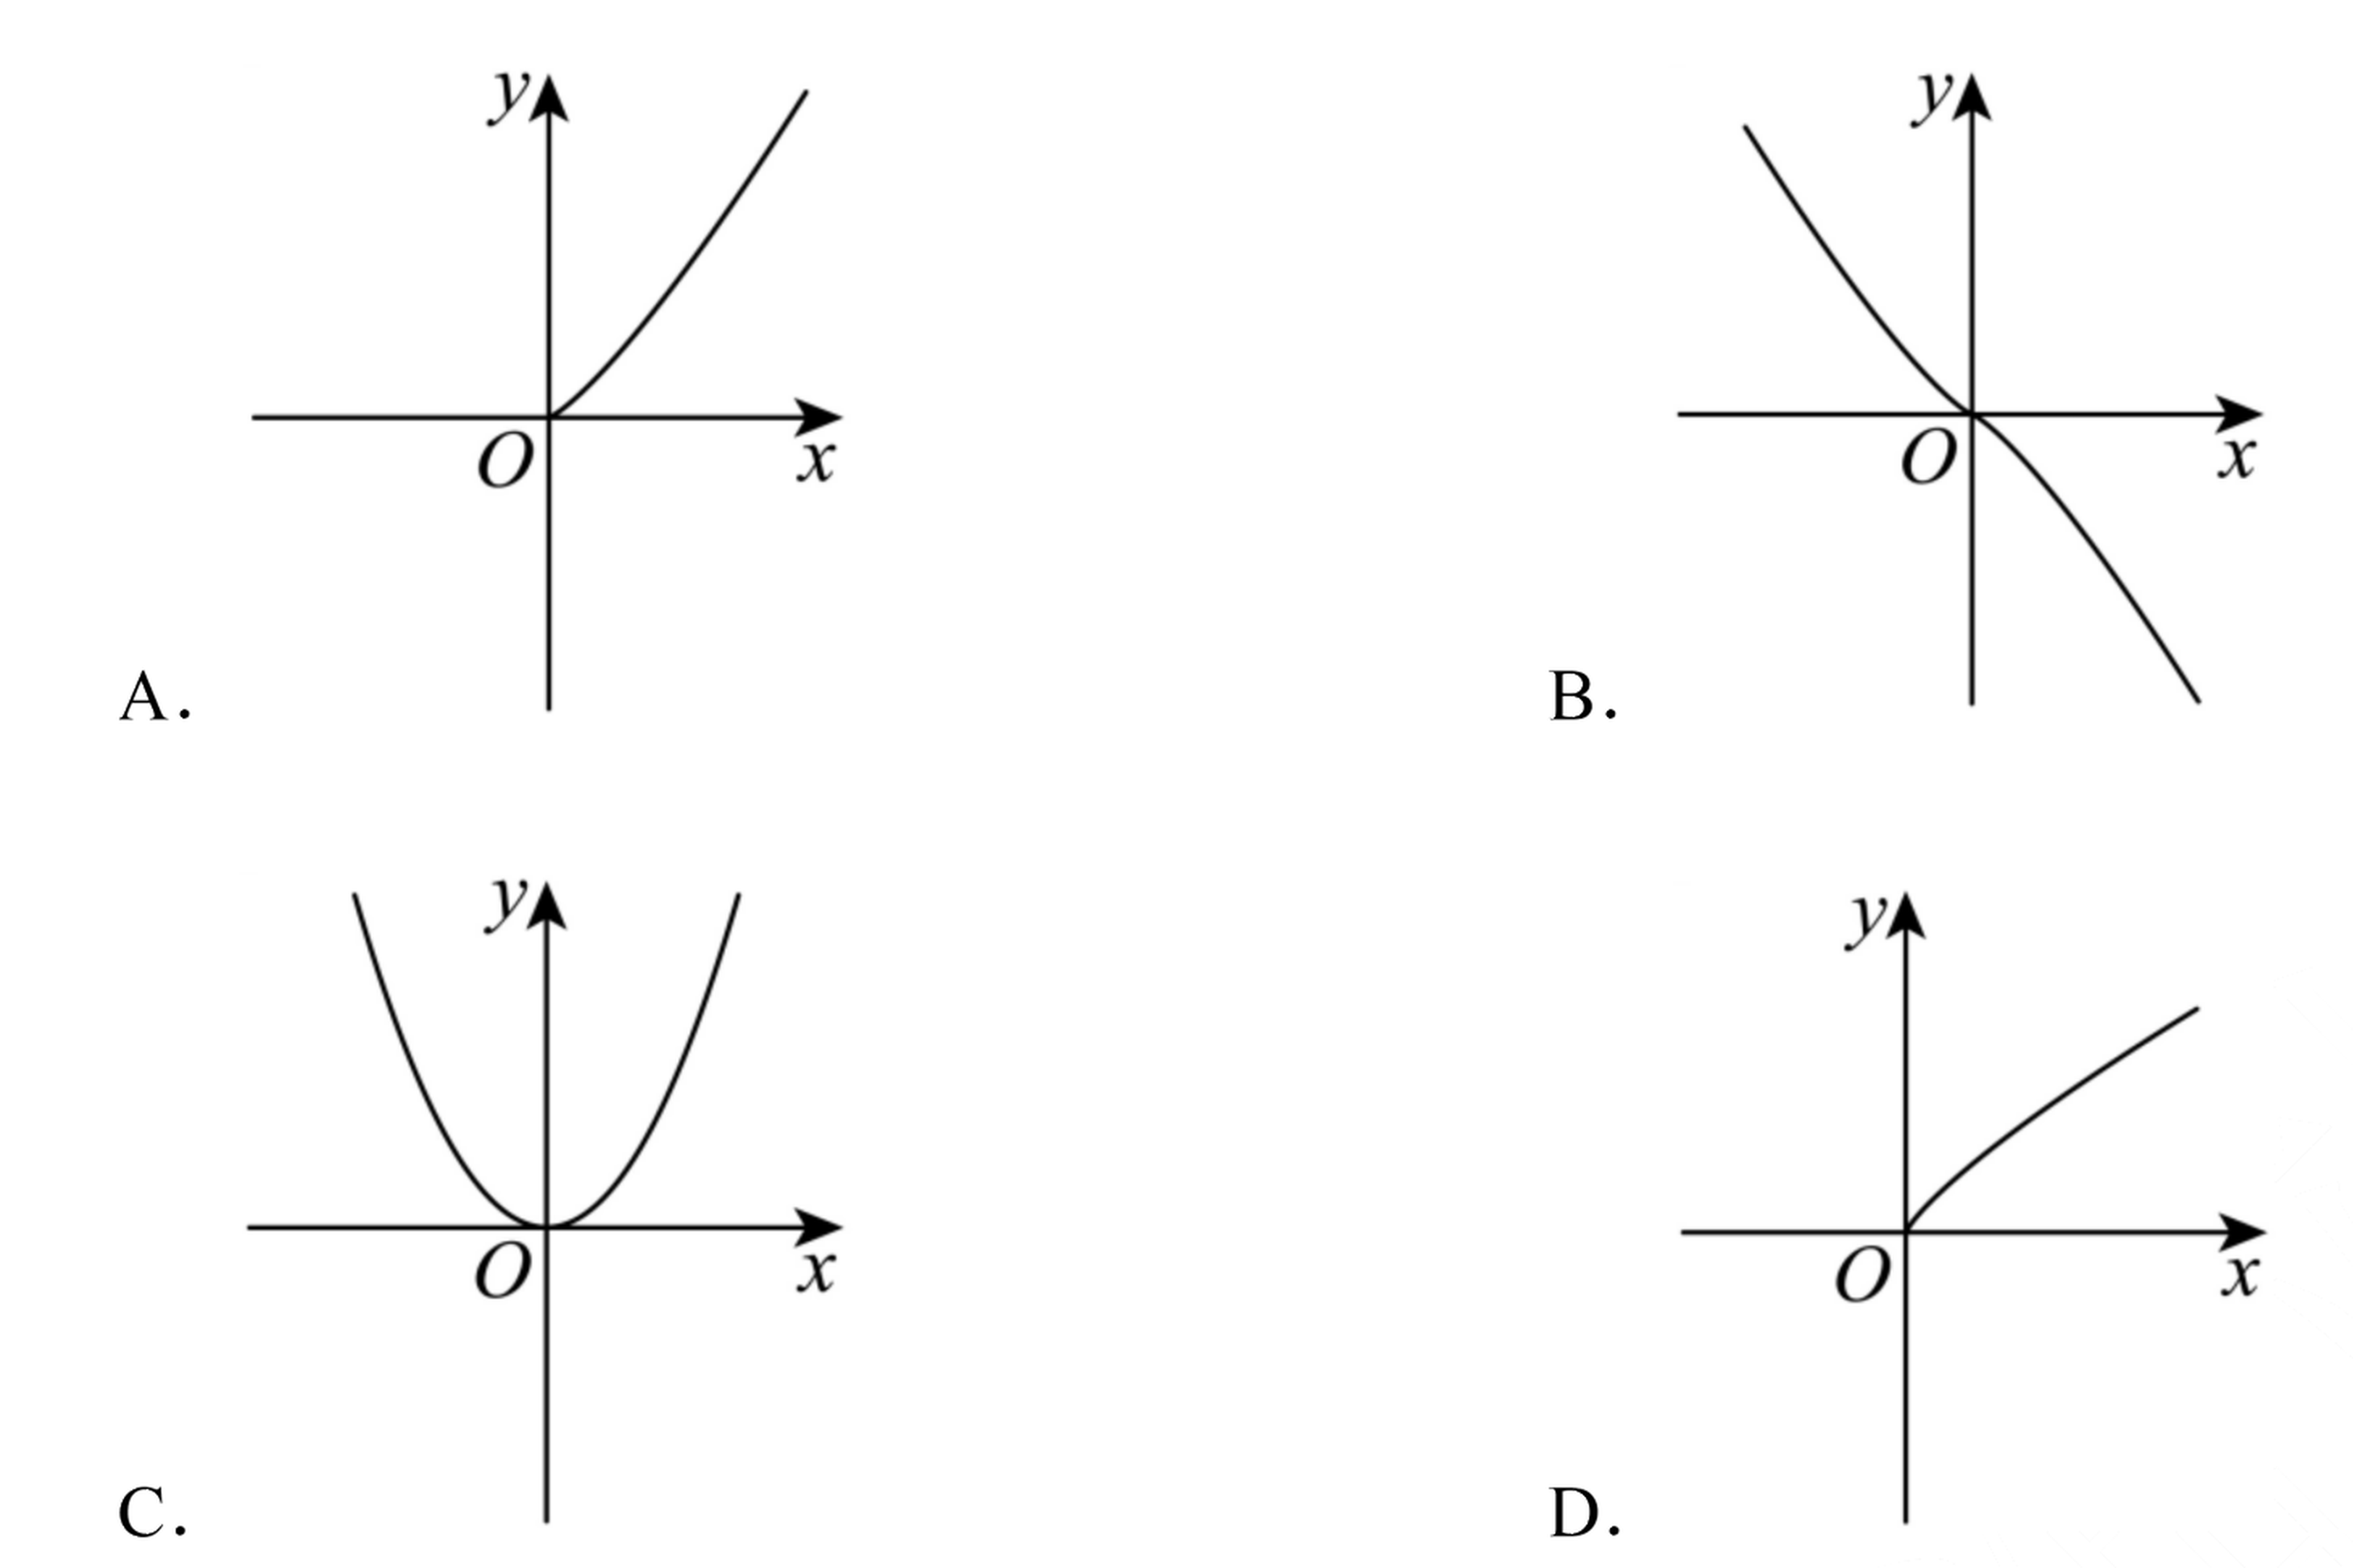
\includegraphics[width=0.80\textwidth]{figures/gao136_q13.png}
\end{center}

\ifanswer
\solbegin
\step{由 $y=x^{\frac54}=\sqrt[4]{x^5}$，函数的定义域为 $[0,+\infty)$，排除 BC，}% 原卷"排除 BC"连写，照录
\step{因为 $\dfrac54>1$，所以函数 $y=x^{\frac54}$ 的图象呈现下凸的趋势，排除 D. 故选 $A$.}
\solend
\fi

\item 下列不等式① $a+\dfrac1a\geqslant2$；② $a^2+4\geqslant4a$；③ $\left\lvert\dfrac ba+\dfrac ab\right\rvert\geqslant2$；④ $\dfrac{2a^2b^2}{a^2+b^2}\leqslant ab$；其中恒成立的是\mbox{（\quad）}

\keepwithprev
A. ①④\qquad B. ③④\qquad C. ②③\qquad D. ①②

\ifanswer
\ans{$C$}
\fi

\item 函数 $y=a^x+b-1(a>0,a\neq1)$ 单调递增且图象不经过第四象限，则 $a,b$ 满足的条件为\mbox{（\quad）}

\keepwithprev
A. $a>1,b\leqslant1$\qquad B. $a>1,b\geqslant0$\qquad C. $0<a<1,b\leqslant1$\qquad D. $0<a<1,b\geqslant1$

\ifanswer
\solbegin
\step{因为函数 $y=a^x+b-1$ 单调递增，所以 $a>1$，}
\step{图象不经过第四象限，则 $x=0$ 时，$y=b\geqslant0$，所以 $a>1,b\geqslant0$，故选 $B$.}
\solend
\fi

\item 设关于 $x$ 的不等式 $\dfrac{ax-1}{x^2-a}<0$ 的解集为 $S$，且 $3\in S$，$4\notin S$，则实数 $a$ 的取值范围为\mbox{（\quad）}

\keepwithprev
A. $(-\infty,-\sqrt3)\cup\left(\dfrac13,\sqrt3\right)$\qquad B. $\left(-\infty,\dfrac14\right)\cup(16,+\infty)$

C. $\left[\dfrac14,\dfrac13\right)\cup(9,16]$\qquad D. 不能确定

\ifanswer
\solbegin
\step{若 $3\in S$，则 $\dfrac{3a-1}{9-a}<0$，解得 $a\in\left(-\infty,\dfrac13\right)\cup(9,+\infty)$，}
\step{若 $4\notin S$，则 $16-a=0$ 或 $\dfrac{4a-1}{16-a}\geqslant0$，解得 $a\in\left[\dfrac14,16\right]$，}
\step{故实数 $a$ 的取值范围为 $\left[\dfrac14,\dfrac13\right)\cup(9,16]$，故选 $C$.}
\solend
\fi

\end{enumerate}

\bigsec{三、解答题}

\begin{enumerate}
\setcounter{enumi}{16}

\item 计算：(1) 计算 $\dfrac{\lg8+\lg125-\lg2-\lg5}{\lg\sqrt{10}\cdot\lg0.1}$；(2) 若 $a^{2x}=2(a>0)$，求 $\dfrac{a^{3x}+a^{-3x}}{a^x+a^{-x}}$.

\ifanswer
\solbegin
\step{(1) 原式 $=\dfrac{2-1}{\frac12\cdot(-1)}=-2$；(2) 原式 $=a^{2x}-1+a^{-2x}=2-1+\dfrac12=\dfrac32$.}
\solend
\fi

\item 不等式 $\dfrac{x-1}{x+1}\geqslant0$ 的解集为 $A$，不等式 $(x-a-1)(2a-x)>0(a<1)$ 的解集为 $B$.

(1) 求集合 $A$；

(2) 若 $B\subseteq A$，求实数 $a$ 的取值范围.

\ifanswer
\solbegin
\step{(1) $A=(-\infty,-1)\cup[1,+\infty)$.}
\step{(2) 由 $(x-a-1)(2a-x)>0(a<1)$，得 $(x-a-1)(x-2a)<0(a<1)$，}
\step{因为 $a<1$，所以 $a+1>2a$，所以 $B=(2a,a+1)$，}
\step{因为 $B\subseteq A$，所以 $2a\geqslant1$ 或 $a+1\leqslant-1$，即 $a\geqslant\dfrac12$ 或 $a\leqslant-2$，}
\step{而 $a<1$，所以实数 $a$ 的取值范围 $(-\infty,-2]\cup\left[\dfrac12,1\right)$.}% 原卷"取值范围"后脱"是／为"，照录
\solend
\fi

\item 已知幂函数 $y=x^m(m\in\R)$ 经过点 $\left(4,\dfrac12\right)$.

(1) 求此幂函数的表达式和定义域；

(2) 已知点 $A(a+2,y_1)$，点 $B(3-2a,y_2)(a\in\R)$ 在此幂函数的图像上，且满足 $y_1<y_2$，求实数 $a$ 的取值范围.

\ifanswer
\solbegin
\step{(1) 幂函数 $y=x^m(m\in\R)$ 经过点 $\left(4,\dfrac12\right)$，所以 $4^m=\dfrac12\Rightarrow m=-\dfrac12$，}
\step{所以 $f(x)=x^{-\frac12}$，定义域为 $(0,+\infty)$.}
\step{(2) 由于函数 $f(x)$ 在其定义域 $(0,+\infty)$ 上严格减，}
\step{由 $y_1<y_2$，得 $a+2>3-2a\geqslant0\Rightarrow a\in\left(\dfrac13,\dfrac32\right]$.}
\solend
\fi

% 第 20 题图取 05 页截图（0.42\textwidth、高约 6cm）。试排 \item 前加 7cm 守卫会多出
% 一张只有两行正文的稀疏页，且三版不加守卫时图均与题干、【解析】同页，故不另加守卫
\item 某医药研究所开发一种抗甲流新药，如果成年人按规定的剂量服用，据监测：服药后每毫升血液中的含药量 $y$（微克）与时间 $t$（小时）之间近似满足如图所示的曲线.

(1) 结合图，求 $k$ 与 $a$ 的值；

(2) 写出服药后 $y$ 与 $t$ 之间的函数关系式 $y=f(t)$；

(3) 据进一步测定：每毫升血液中含药量不少于 $0.5$ 微克时治疗疾病有效，求服药一次治疗有效的时间范围？

\begin{center}
% 图取原卷 05 页截图去粉色水印、去色，3x LANCZOS 放大
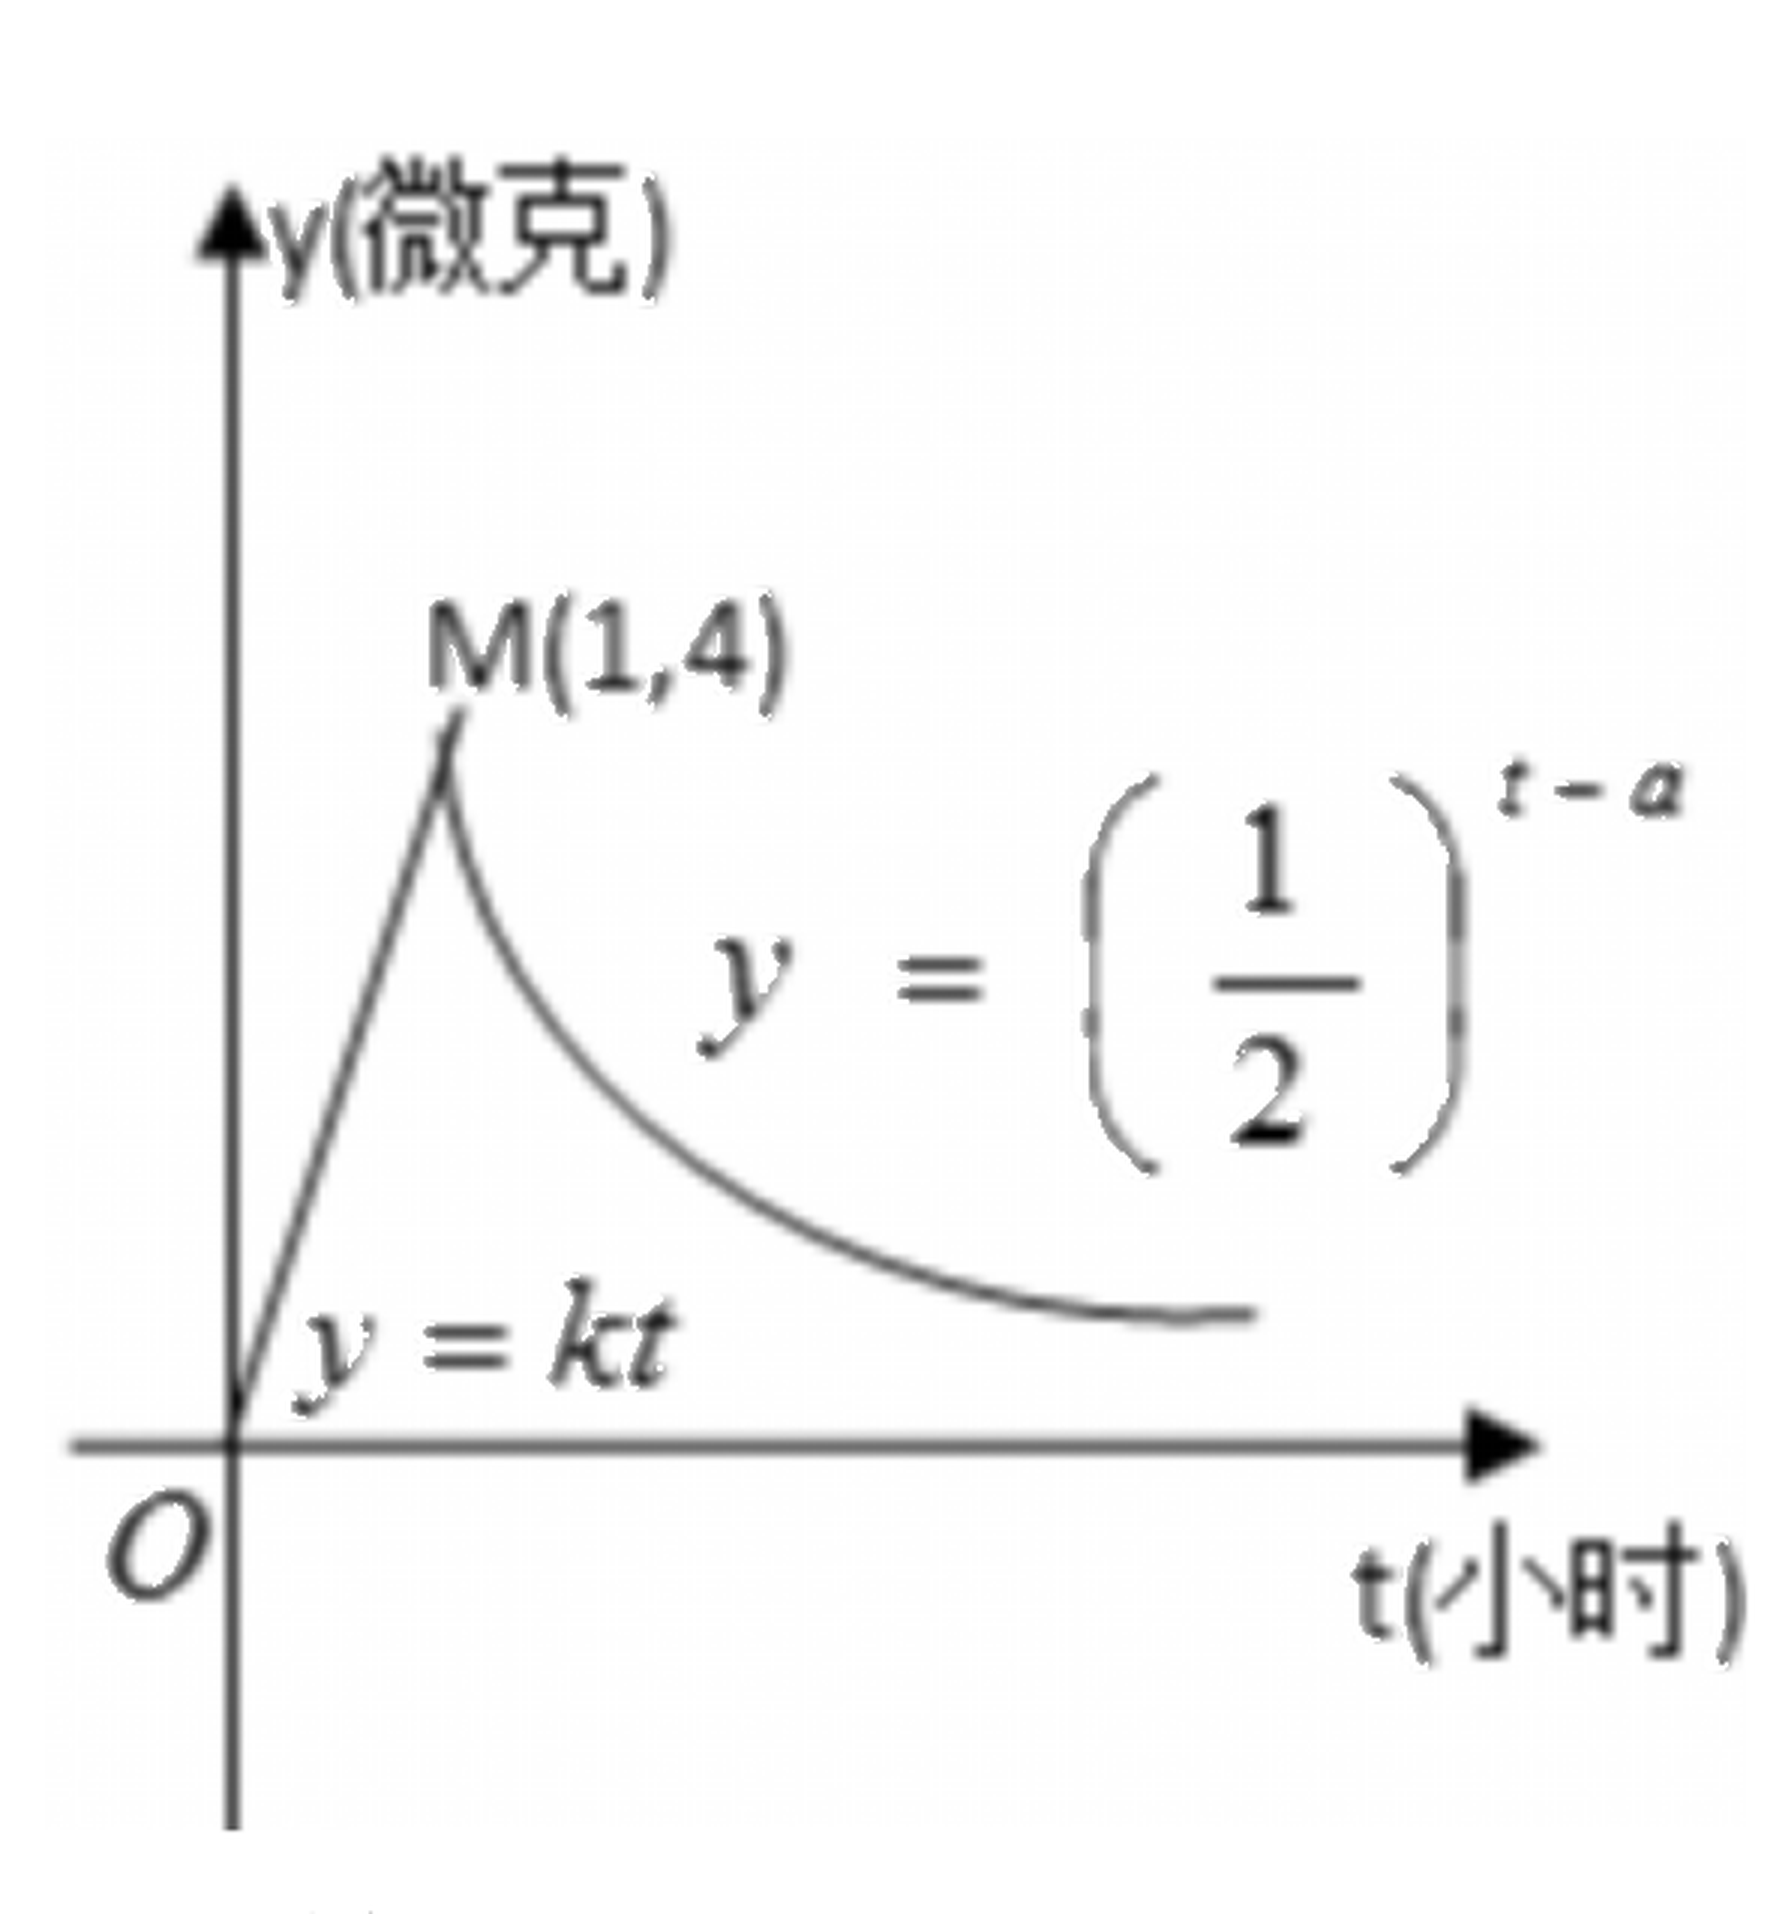
\includegraphics[width=0.42\textwidth]{figures/gao136_q20.png}
\end{center}

\ifanswer
\solbegin
\step{(1) 当 $0\leqslant t\leqslant1$ 时，函数图象是一条线段，由于过原点与点 $(1,4)$，所以 $k=4$，}
\step{其解析式为 $y=4t$，$0\leqslant t\leqslant1$；}
\step{当 $t\geqslant1$ 时，函数的解析式为 $y=\left(\dfrac12\right)^{t-a}$，}
\step{此时 $M(1,4)$ 在曲线上，将此点的坐标代入函数解析式得 $4=\left(\dfrac12\right)^{1-a}$，}
\step{解得 $a=3$；}
\step{(2) 由 (1) 得 $f(t)=\begin{cases}4t,0\leqslant t\leqslant1\\\left(\frac12\right)^{t-3},t>1\end{cases}$；}
\step{(3) 由 (2) 得，令 $f(t)\geqslant0.5$，即 $\begin{cases}4t\geqslant0.5,0\leqslant t\leqslant1\\\left(\frac12\right)^{t-3}\geqslant0.5,t>1\end{cases}$，所以 $\dfrac18\leqslant t\leqslant4$.}
\solend
\fi

\item 已知关于 $x$ 的不等式 $(kx-k^2-4)(x-4)>0$，其中 $k\in\R$.

(1) 当 $k=-1$，求不等式的解集 $A$；

(2) 当 $k$ 变化时，试求不等式的解集 $A$；

(3) 对于不等式解集 $A$，满足 $A\cap\Z=B$. 试探究集合 $B$ 能否为有限集，若能，求出使得集合 $B$ 中元素最少的 $k$ 的所有取值，并用列举法表示此时的集合 $B$，若不能，说明理由；

\ifanswer
\solbegin
\step{(1) 当 $k=-1$ 时，原不等式可化为 $(x+5)(x-4)<0$，}
\step{解得 $-5<x<4$，故不等式的解集为 $\{x\mid -5<x<4\}$；}
\step{(2) 当 $k=0$ 时，解集为 $\{x\mid x<4\}$，}
\step{当 $k>0$ 时，$\dfrac{k^2+4}{k}=k+\dfrac4k\geqslant4$，解集为 $\{x\mid x<4\text{ 或 }x>\dfrac{k^2+4}{k}\}$；}
\step{当 $k<0$ 时，解集为 $\{x\mid \dfrac{k^2+4}{k}<x<4\}$，}
\step{综上，当 $k=0$ 时，$A=\{x\mid x<4\}$，}
\step{当 $k>0$ 时，$A=\{x\mid x<4\text{ 或 }x>\dfrac{k^2+4}{k}\}$；}
\step{当 $k<0$ 时，$A=\{x\mid \dfrac{k^2+4}{k}<x<4\}$，}
\step{(3) 由 (2) 得当 $k\geqslant0$ 时，$B$ 为无限集，当 $k<0$ 时，$B$ 为有限集，}
\step{此时，$\dfrac{k^2+4}{k}=k+\dfrac4k\leqslant-4$，当且仅当 $k=-2$ 时取等号，}
\step{所以 $k=-2$ 时，$B$ 中元素最少，此时 $A=\{x\mid -4<x<4\}$，}
\step{所以 $B=\{-3,-2,-1,0,1,2,3\}$.}
\solend
\fi

\end{enumerate}

% 第 22 题是"四、附加题"首题且带 9cm 图块，守卫须放在 \bigsec 之前连节标题一起量，
% 否则"四、附加题"会孤立在页末（B 类，照 高一26／40／59 成例）
\needvspace{11cm}
\bigsec{四、附加题}

\begin{enumerate}
\setcounter{enumi}{21}

% 第 22 题四幅抛物线/坐标图选项是一整块，守卫放在 \item 之前
\needvspace{9cm}
\item 函数 $f(x)=\left(\dfrac12\right)^{\lvert x+1\rvert}$ 的图象大致为\mbox{（\quad）}

\keepwithprev
\begin{center}
% 四幅抛物线/坐标图选项取原卷 07 页截图去粉色水印，按原卷 2x2 排布合并为一张
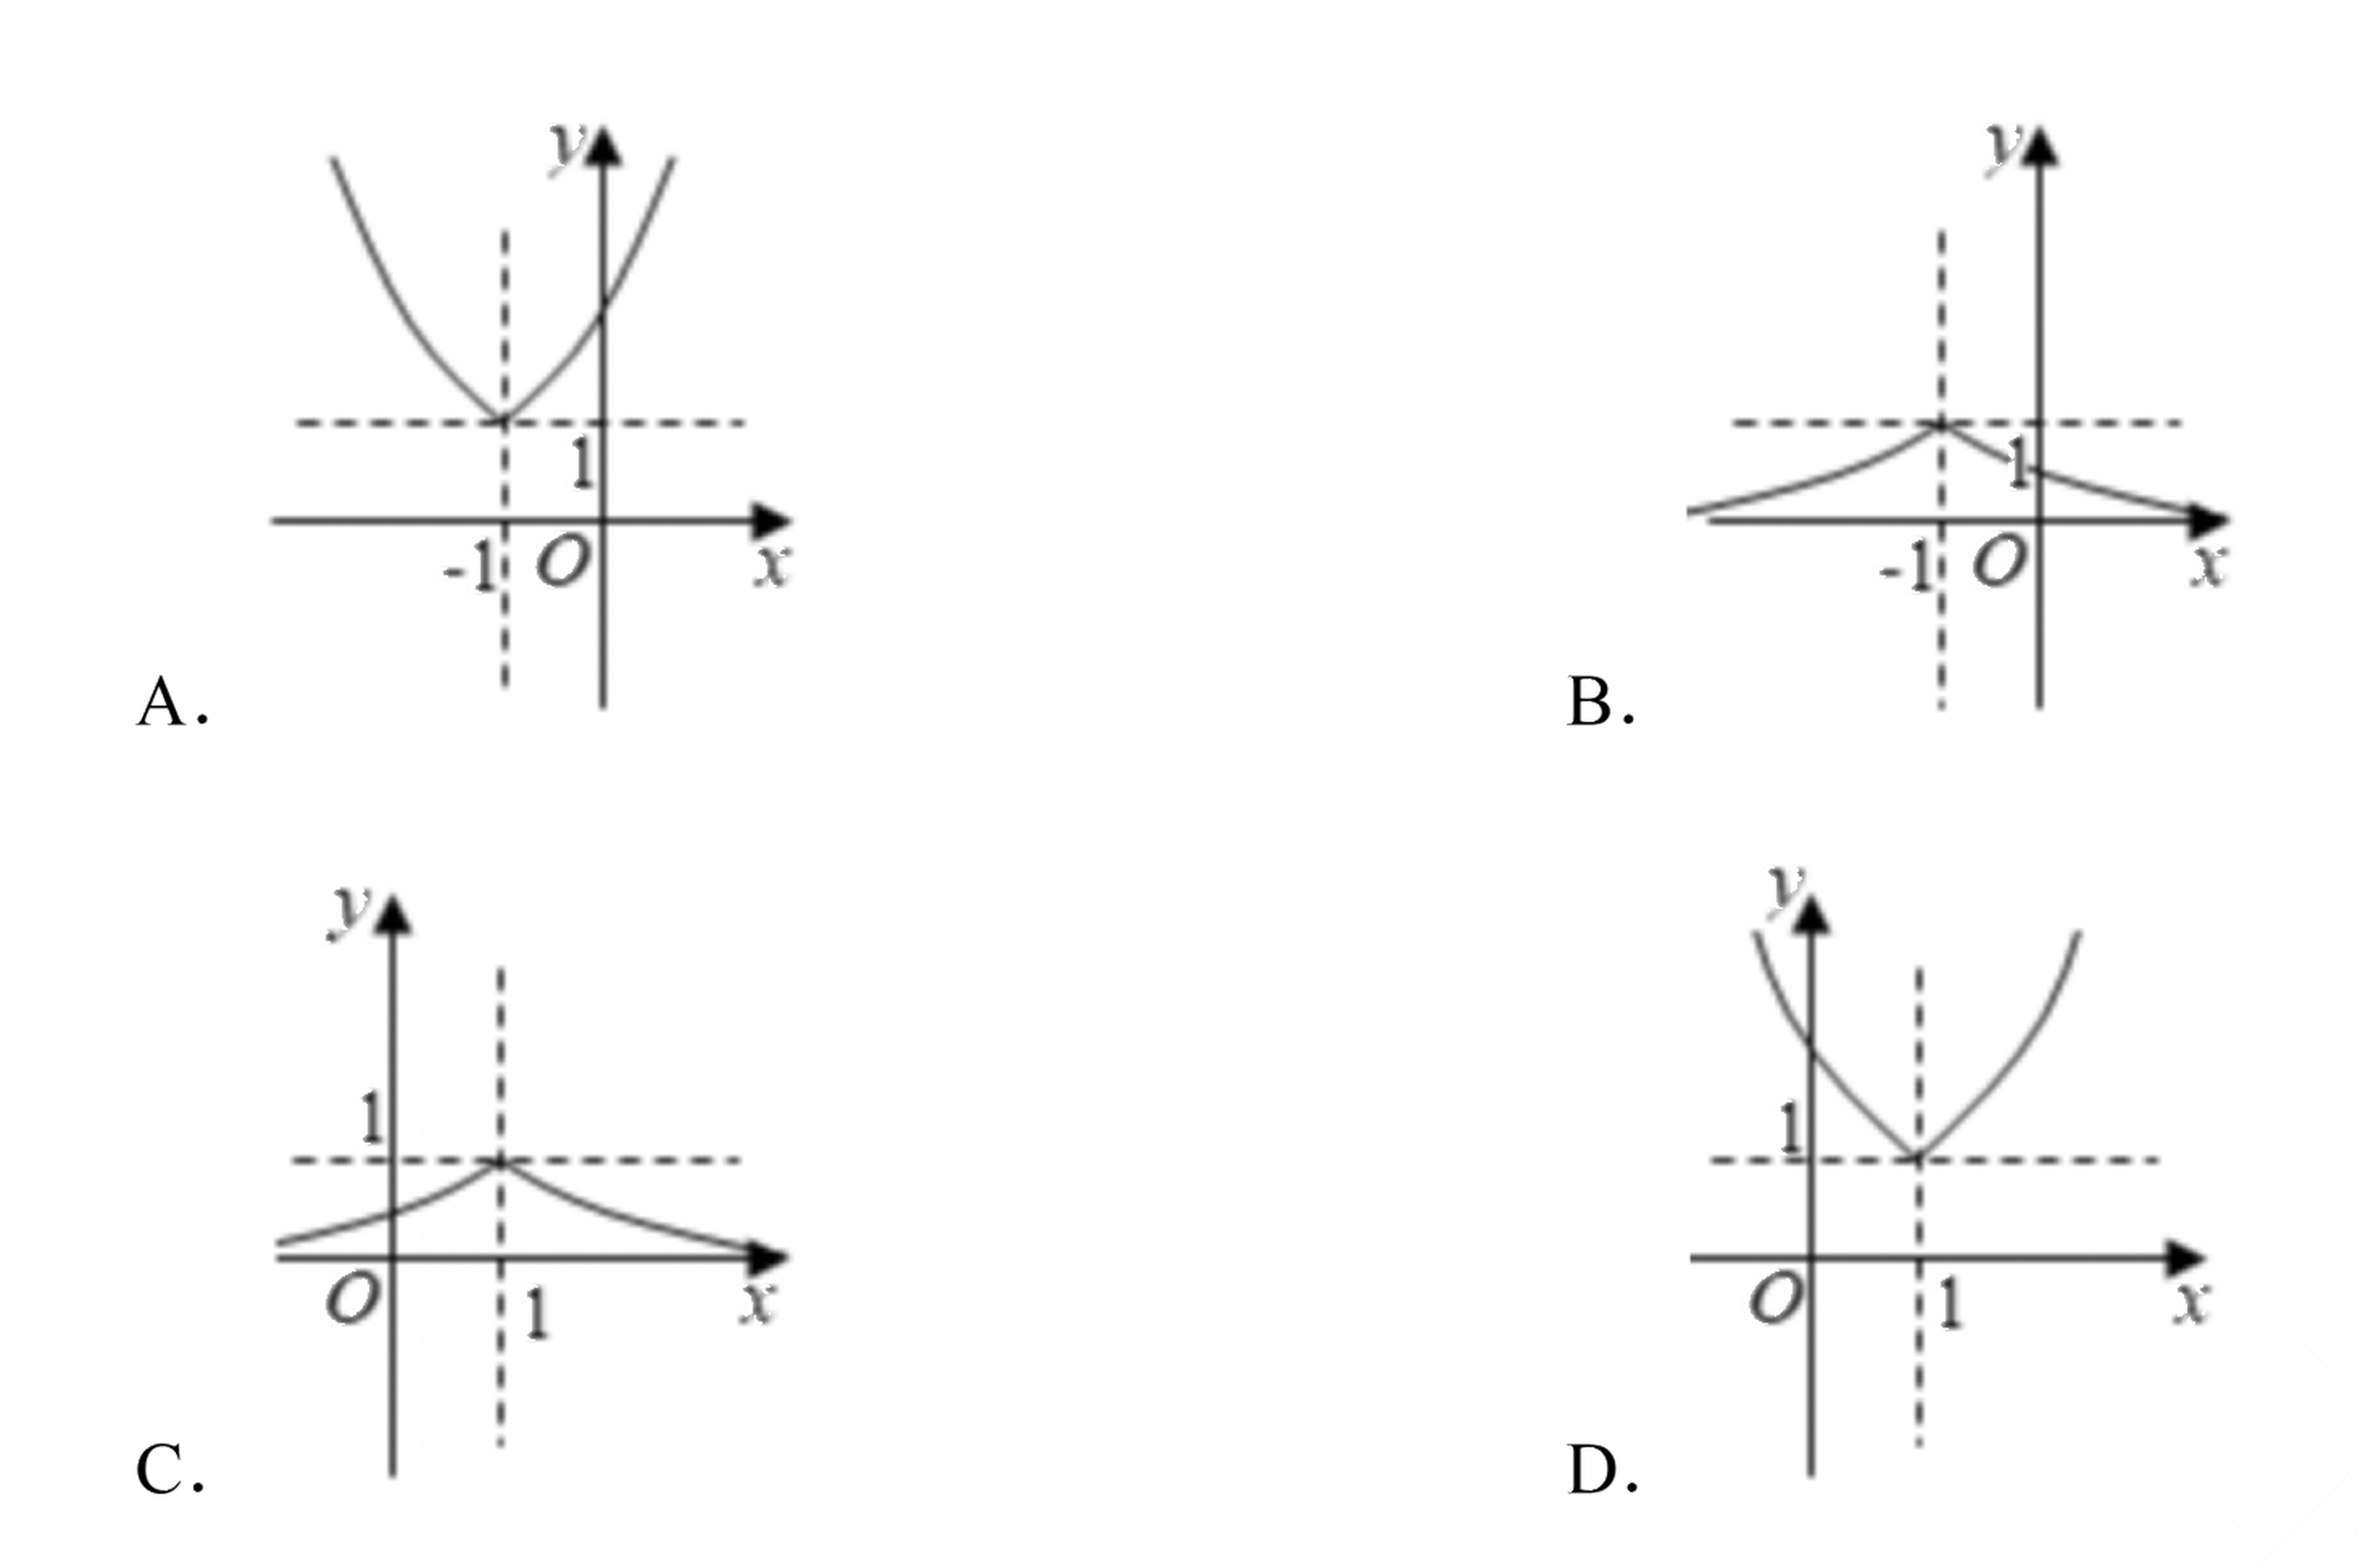
\includegraphics[width=0.80\textwidth]{figures/gao136_q22.png}
\end{center}

\ifanswer
\ans{$B$}
\fi

\end{enumerate}

\end{document}
"
% 紧凑版：xelatex "\def\iscompact{1}% 高一136_三林中学_期中.tex
%   —— 高一上数学"2026-2027 年三林中学高一上期中"（试卷版/答案版）
% 试卷版：xelatex 高一136_三林中学_期中.tex
% 答案版：xelatex "\def\isanswer{1}\input{高一136_三林中学_期中.tex}"
% 紧凑版：xelatex "\def\iscompact{1}\input{高一136_三林中学_期中.tex}"
%
% ① 原始材料：微信公众号"魔都数学加油站"文章，作者破晓，2026-11-15 18:04 发布；
% 连载"27学年高一136"，原文标题"27学年高一136——2026-2027年上海市三林中学高一上期中"；
% 原文链接：https://mp.weixin.qq.com/s/jaMzqMm6pDvcT0yM0d7eaQ。
% 正文为 7 张 PNG 页（01、04、06 为 4762x6735；02、03、05、07 为 2560x3620，
% 同一篇各页分辨率不同，逐页按各自分辨率裁图核对），题目下印有【答案】或【解析】，为讲评版。
% 题目、解析均据原图转录；卷面粉红色水印"魔都数学加油站"及公众号页脚未录入。
% 全卷 3 幅插图：第 13 题四幅坐标图选项（03 页）、第 20 题药物浓度折线/曲线图（05 页）、
% 第 22 题四幅抛物线/坐标图选项（07 页），均取原卷截图去粉色水印、去色、LANCZOS 放大，
% 四幅选项按原卷 2x2 排布合并为一张；图前按惯例加 \needvspace 守卫。
%
% 卷首标题：原卷印作"2026-2027 年三林中学高一上期中"（公众号标题中的"上海市"
% 卷面标题行没有，本稿照卷面），年份区间按全稿惯例排 en dash；原卷未印副标题，
% 本卷为期中卷、跨集合与常用逻辑用语／不等式／函数三章，按题目内容标为
% "集合与常用逻辑用语、不等式、函数"（与 125／126／128／129／131／132／133 同期中卷口径相同）：
% 集合与逻辑见 Q3、Q6、Q10、Q12、Q16、Q18、Q21，不等式见 Q5、Q7、Q8、Q9、Q14、Q15，
% 函数（幂函数、指数／对数、基本不等式应用）见 Q4、Q11、Q13、Q17、Q19、Q20、Q22。
%
% 题号体例：本卷共 20 题——一、填空题 3—12（10 题）、二、选择题 13—16（4 题）、
% 三、解答题 17—21（5 题）、四、附加题 22（1 题）。四节分别
% \setcounter{enumi}{2}／{12}／{16}／{21}。
%
% ② 与原卷的排版差异：
%   ① 原文从第 3 题起，本稿保留原题号；末节"四、附加题"另起 \bigsec，题号续到 22；
%   ② 原卷每题下直接印【答案】或【解析】，本稿按全稿惯例置于答案版；第 3、4、6 题只印
%      【答案】、无【解析】，提 \ans{}；第 14 题答案 C 印在题干括号内、无【解析】，按
%      高一53／高一108／高一132／高一133 成例括号留空、另提 \ans{$C$}；第 22 题答案 B
%      印在题干括号内、无【解析】，同例提 \ans{$B$}；第 13、15、16 题答案在解析末句
%      "故选 …"，括号内留空、不另提 \ans{}；其余各题印【解析】、无独立答案段；
%   ③ 原卷未印副标题，本稿按"知识模块"口径补出；
%   ④ 原卷填空横线按全稿惯例排为 \blankline[4.4em]；选择题括号排 \mbox{（\quad）}、
%      每个选项段前按惯例加 \keepwithprev（四幅图选项那一枚放在 \begin{center} 之前）；
%      解答题不留作答区、不加 \anspace（原卷为讲评版，与 129／131／132／133 同）；
%   ⑤ 原卷数集排斜体 $R$／$R^+$／$Z$，按全稿惯例改 \R／\R^+／\Z；空集记号 \varnothing；
%      绝对值排 \lvert…\rvert，集合描述竖线排 \mid；不等号按全稿惯例排 \leqslant／\geqslant；
%   ⑥ 子题标号 (1)(2)(3) 原卷用半角括号，照录；圈数字 ①②③④ 照录；第 12 题甲／乙／丙
%      三行与第 14 题四个编号不等式照录；
%   ⑦ 数学式内半角逗号照录（如 Q4"$a>0,a\neq1$"、Q6"$\{(-2,4),(1,1)\}$"、
%      Q7"$a=2+3=5,b=2\times3=6$"、Q11"$x_1,x_2$"、Q12"$m,n\in R^+$"、
%      Q15"$a>1,b\geq0$"、Q18"$B=(2a,a+1)$"、Q20"$4t,0\leq t\leq1$"、
%      Q21"$\{-3,-2,-1,0,1,2,3\}$"）；原卷行末西文句点照录，行中全角逗号照录；
%   ⑧ 三幅插图：第 13 题四幅坐标图选项合并裁为一张 \includegraphics（题前 \needvspace{9cm}）；
%      第 20 题折线/曲线图取 05 页截图（0.42\textwidth）；第 22 题四幅抛物线/坐标图选项合并
%      裁为一张（题前 \needvspace{9cm}）。第 13、22 题分别是"二、选择题""四、附加题"的首题
%      且带大图块，另在两处 \bigsec 之前各加 \needvspace{11cm} 连节标题一起量，避免节标题
%      孤立在页末（切页审计 B 类；照 高一26／40／59 成例）。第 20 题图不是节首题、三版试排
%      图均与题干同页，加 7cm 守卫反会多出一张只有两行正文的稀疏页，故不另加守卫；
%      三版切页审计均"合计异常：无"（试卷 4 页／紧凑 4 页／答案 6 页）；
%   ⑨ 跨页续印按题合并：Q16 题干在 03 页、括号与选项及【解析】在 04 页；Q19 题干在 04 页、
%      (2) 与【解析】在 05 页；Q20 (3)【解析】在 06 页；Q22 四幅图在 07 页；本稿按题连排；
%   ⑩ 题干中的中文弯引号按原卷照录，注释内一律 ASCII 引号；原卷"图像／图象"两种写法混用，
%      逐处照录（Q4、Q19 作"图像"，Q13、Q15、Q20、Q22 作"图象"）；
%   ⑪ 附加题节：原卷印"四、附加题"，本稿用 \bigsec{四、附加题} 另起一节、
%      \setcounter{enumi}{21}，顶层 1 个 \item（与 高一09／15／16／22／35／39／47／61 同口径）；
%      Q22 只印括号内答案、提 \ans{}，不计入 \step 账。
%
% 判别式字形：全卷仅第 9 题【解析】cases 块出现判别式"$\Delta=a^2-8a<0$"，原卷印
%   等腰、偏高的三角 $\Delta$，逐处放大核对并照录 \Delta；全卷未出现扁等边三角 \triangle。
%
% 子集符号：第 18 题 (2) 题干"$B\subseteq A$"与【解析】"$B\subseteq A$"两处原卷均印
%   带下划线 $\subseteq$，逐处放大核对、照录 \subseteq；全卷未出现单线 \subset。
%
% 原卷存疑照录（均照录未改，正文对应处另有 % 注）：
%   第 12 题乙行"$\dfrac{m+n}{mm}=\dfrac1{mn}$"前一分母印作 $mm$（后一处作 $mn$），照录；
%   第 12 题【解析】"$\geqslant\dfrac1{100}\left[a^2+1+2\sqrt{a^2}\right]$"保留 $\sqrt{a^2}$
%      未化简为 $a$，照录；
%   第 13 题【解析】"排除 BC"与"排除 D"连写选项字母，照录；
%   第 18 题 (2)【解析】末行"所以实数 $a$ 的取值范围 $(-\infty,-2]\cup[\frac12,1)$"
%      "取值范围"后脱"是／为"字，照录；
%   第 21 题 (3) 题干"求出使得集合 $B$ 中元素最少的 $k$ 的所有取值"而【解析】只给出
%      $k=-2$ 一处，措辞照录。
%
% 行数复核：逐题数 \step 条数，合计 51 条（Q3：0；Q4：0；Q5：2；Q6：0；Q7：2；Q8：1；
% Q9：1；Q10：4；Q11：1；Q12：4；Q13：2；Q14：0；Q15：2；Q16：3；Q17：1；Q18：5；
% Q19：4；Q20：7；Q21：12；Q22：0），与原卷印刷行逐题相等（cases 块作一个印刷行计）。
% 第 3、4、6、14、22 题只印【答案】、提 \ans{}，不计入 \step 账；第 13、15、16 题答案在
% 解析末句，括号内留空、不另提 \ans{}。
%
\documentclass[a4paper,11pt]{article}
\usepackage{common}

\begin{document}

\examtitlest[3]{2026--2027 年三林中学高一上期中}{集合与常用逻辑用语、不等式、函数}

\bigsec{一、填空题}

\begin{enumerate}
\setcounter{enumi}{2}

\item 用反证法证明命题“若 $x+y\neq5$，则 $x\neq2$ 或 $y\neq3$”为真命题时，第一个步骤是\blankline[4.4em].

\ifanswer
\ans{假设 $x=2$ 且 $y=3$}
\fi

\item 函数 $y=a^{x-1}+1(a>0,a\neq1)$ 的图像恒过定点 $A$，则点的坐标是\blankline[4.4em].

\ifanswer
\ans{$(1,2)$}
\fi

\item 已知 $x>1$，则 $x+\dfrac4{x-1}$ 的最小值是\blankline[4.4em].

\ifanswer
\solbegin
\step{由 $x>1$，得 $x-1>0$，则 $x+\dfrac4{x-1}=x-1+\dfrac4{x-1}+1\geqslant2\sqrt{(x-1)\cdot\dfrac4{x-1}}+1=5$，}
\step{当且仅当 $x-1=\dfrac4{x-1}$ 即 $x=3$ 时取等号，取得最小值 $5$.}
\solend
\fi

\item 已知集合 $A=\{(x,y)\mid y=x^2\}$，集合 $B=\{(x,y)\mid y=2-x\}$，求 $A\cap B=$\blankline[4.4em].

\ifanswer
\ans{$\{(-2,4),(1,1)\}$}
\fi

\item 已知一元二次不等式 $x^2-ax+b<0$ 的解集为 $(2,3)$，则不等式 $bx^2-ax+1>0$ 的解集是\blankline[4.4em].

\ifanswer
\solbegin
\step{$a=2+3=5,b=2\times3=6$，则 $bx^2-ax+1>0$ 即 $6x^2-5x+1>0$，}
\step{即 $(3x-1)(2x-1)>0$，解集为 $\left(-\infty,\dfrac13\right)\cup\left(\dfrac12,+\infty\right)$.}
\solend
\fi

\item 不等式 $(x+2)^3<(5-2x)^3$ 的解集为\blankline[4.4em].

\ifanswer
\solbegin
\step{由 $(x+2)^3<(5-2x)^3$ 得 $x+2<5-2x$，故解集为 $(-\infty,1)$.}
\solend
\fi

\item 若关于 $x$ 的不等式 $ax^2-ax+2>0$ 的解集为 $\R$，则实数 $a$ 的取值范围是\blankline[4.4em].

\ifanswer
\solbegin
\step{由题意得 $a=0$ 或 $\begin{cases}a>0\\\Delta=a^2-8a<0\end{cases}$，所以 $0\leqslant a<8$.}% 判别式原卷印高三角 $\Delta$，照录
\solend
\fi

\item 已知关于 $x$ 的不等式 $\lvert x+3\rvert+\lvert x-a\rvert\geqslant5$ 恒成立，则实数 $a$ 的取值范围为\blankline[4.4em].

\ifanswer
\solbegin
\step{因为 $\lvert x+3\rvert+\lvert x-a\rvert\geqslant\lvert x-a-x-3\rvert=\lvert 3+a\rvert$，}
\step{要使 $\lvert x+3\rvert+\lvert x-a\rvert\geqslant5$ 恒成立，则 $\lvert a+3\rvert\geqslant5$ 即可，}
\step{所以 $a+3\geqslant5$ 或 $a+3\leqslant-5$，解得 $a\geqslant2$ 或 $a\leqslant-8$，}
\step{即实数 $a$ 的取值范围是 $(-\infty,-8]\cup[2,+\infty)$.}
\solend
\fi

\item 若方程 $\lg^2 x-2\lg x-2=0$ 的两个解为 $x_1,x_2$，求 $\log_{x_1}x_2+\log_{x_2}x_1$ 的值为\blankline[4.4em].

\ifanswer
\solbegin
\step{$\log_{x_1}x_2+\log_{x_2}x_1=\dfrac{\lg x_2}{\lg x_1}+\dfrac{\lg x_1}{\lg x_2}=\dfrac{(\lg x_1+\lg x_2)^2-2\lg x_1\lg x_2}{\lg x_1\lg x_2}=-4$.}
\solend
\fi

\item 三个同学对问题“已知 $m,n\in \R^+$，且 $m+n=1$，求 $\dfrac1m+\dfrac1n$ 的最小值”提出各自的解题思路：

思路：

甲：$\dfrac1m+\dfrac1n=\dfrac{m+n}{m}+\dfrac{m+n}{n}=2+\dfrac nm+\dfrac mn$，可用基本不等式求解；

乙：$\dfrac1m+\dfrac1n=\dfrac{m+n}{mm}=\dfrac1{mn}=\dfrac1{m(1-m)}$，可用二次函数配方法求解；% 原卷前一分母印作 $mm$，照录

丙：$\dfrac1m+\dfrac1n=\left(\dfrac1m+\dfrac1n\right)(m+n)=2+\dfrac nm+\dfrac mn$，可用基本不等式求解；参考上述解题思路，

可求得当 $x=$\blankline[4.4em]时，$y=\dfrac{a^2}{x^2}+\dfrac1{100-x^2}$（$0<x<10$，$a>0$）有最小值.

\ifanswer
\solbegin
\step{$y=\dfrac{a^2}{x^2}+\dfrac1{100-x^2}=\left(\dfrac{a^2}{x^2}+\dfrac1{100-x^2}\right)[x^2+(100-x^2)]\times\dfrac1{100}$}
\step{$=\dfrac1{100}\left[a^2+1+\dfrac{x^2}{100-x^2}+\dfrac{a^2(100-x^2)}{x^2}\right]\geqslant\dfrac1{100}\left[a^2+1+2\sqrt{a^2}\right]$}% 原卷保留 $\sqrt{a^2}$ 未化简，照录
\step{当且仅当 $\dfrac{x^2}{100-x^2}=\dfrac{a^2(100-x^2)}{x^2}$，即 $x=\sqrt{\dfrac{100a}{a+1}}$ 时，}
\step{$y=\dfrac{a^2}{x^2}+\dfrac1{100-x^2}(0<x<10,a>0)$ 有最小值.}
\solend
\fi

\end{enumerate}

% 第 13 题是"二、选择题"首题且带 9cm 图块，守卫须放在 \bigsec 之前连节标题一起量，
% 否则"二、选择题"会孤立在页末（B 类，照 高一26／40／59 成例）
\needvspace{11cm}
\bigsec{二、选择题}

\begin{enumerate}
\setcounter{enumi}{12}

% 第 13 题四幅坐标图选项是一整块，守卫放在 \item 之前
\needvspace{9cm}
\item 下列图象中，最符合函数 $y=x^{\frac54}$ 的图象的是\mbox{（\quad）}

\keepwithprev
\begin{center}
% 四幅坐标图选项取原卷 03 页截图去粉色水印，按原卷 2x2 排布合并为一张
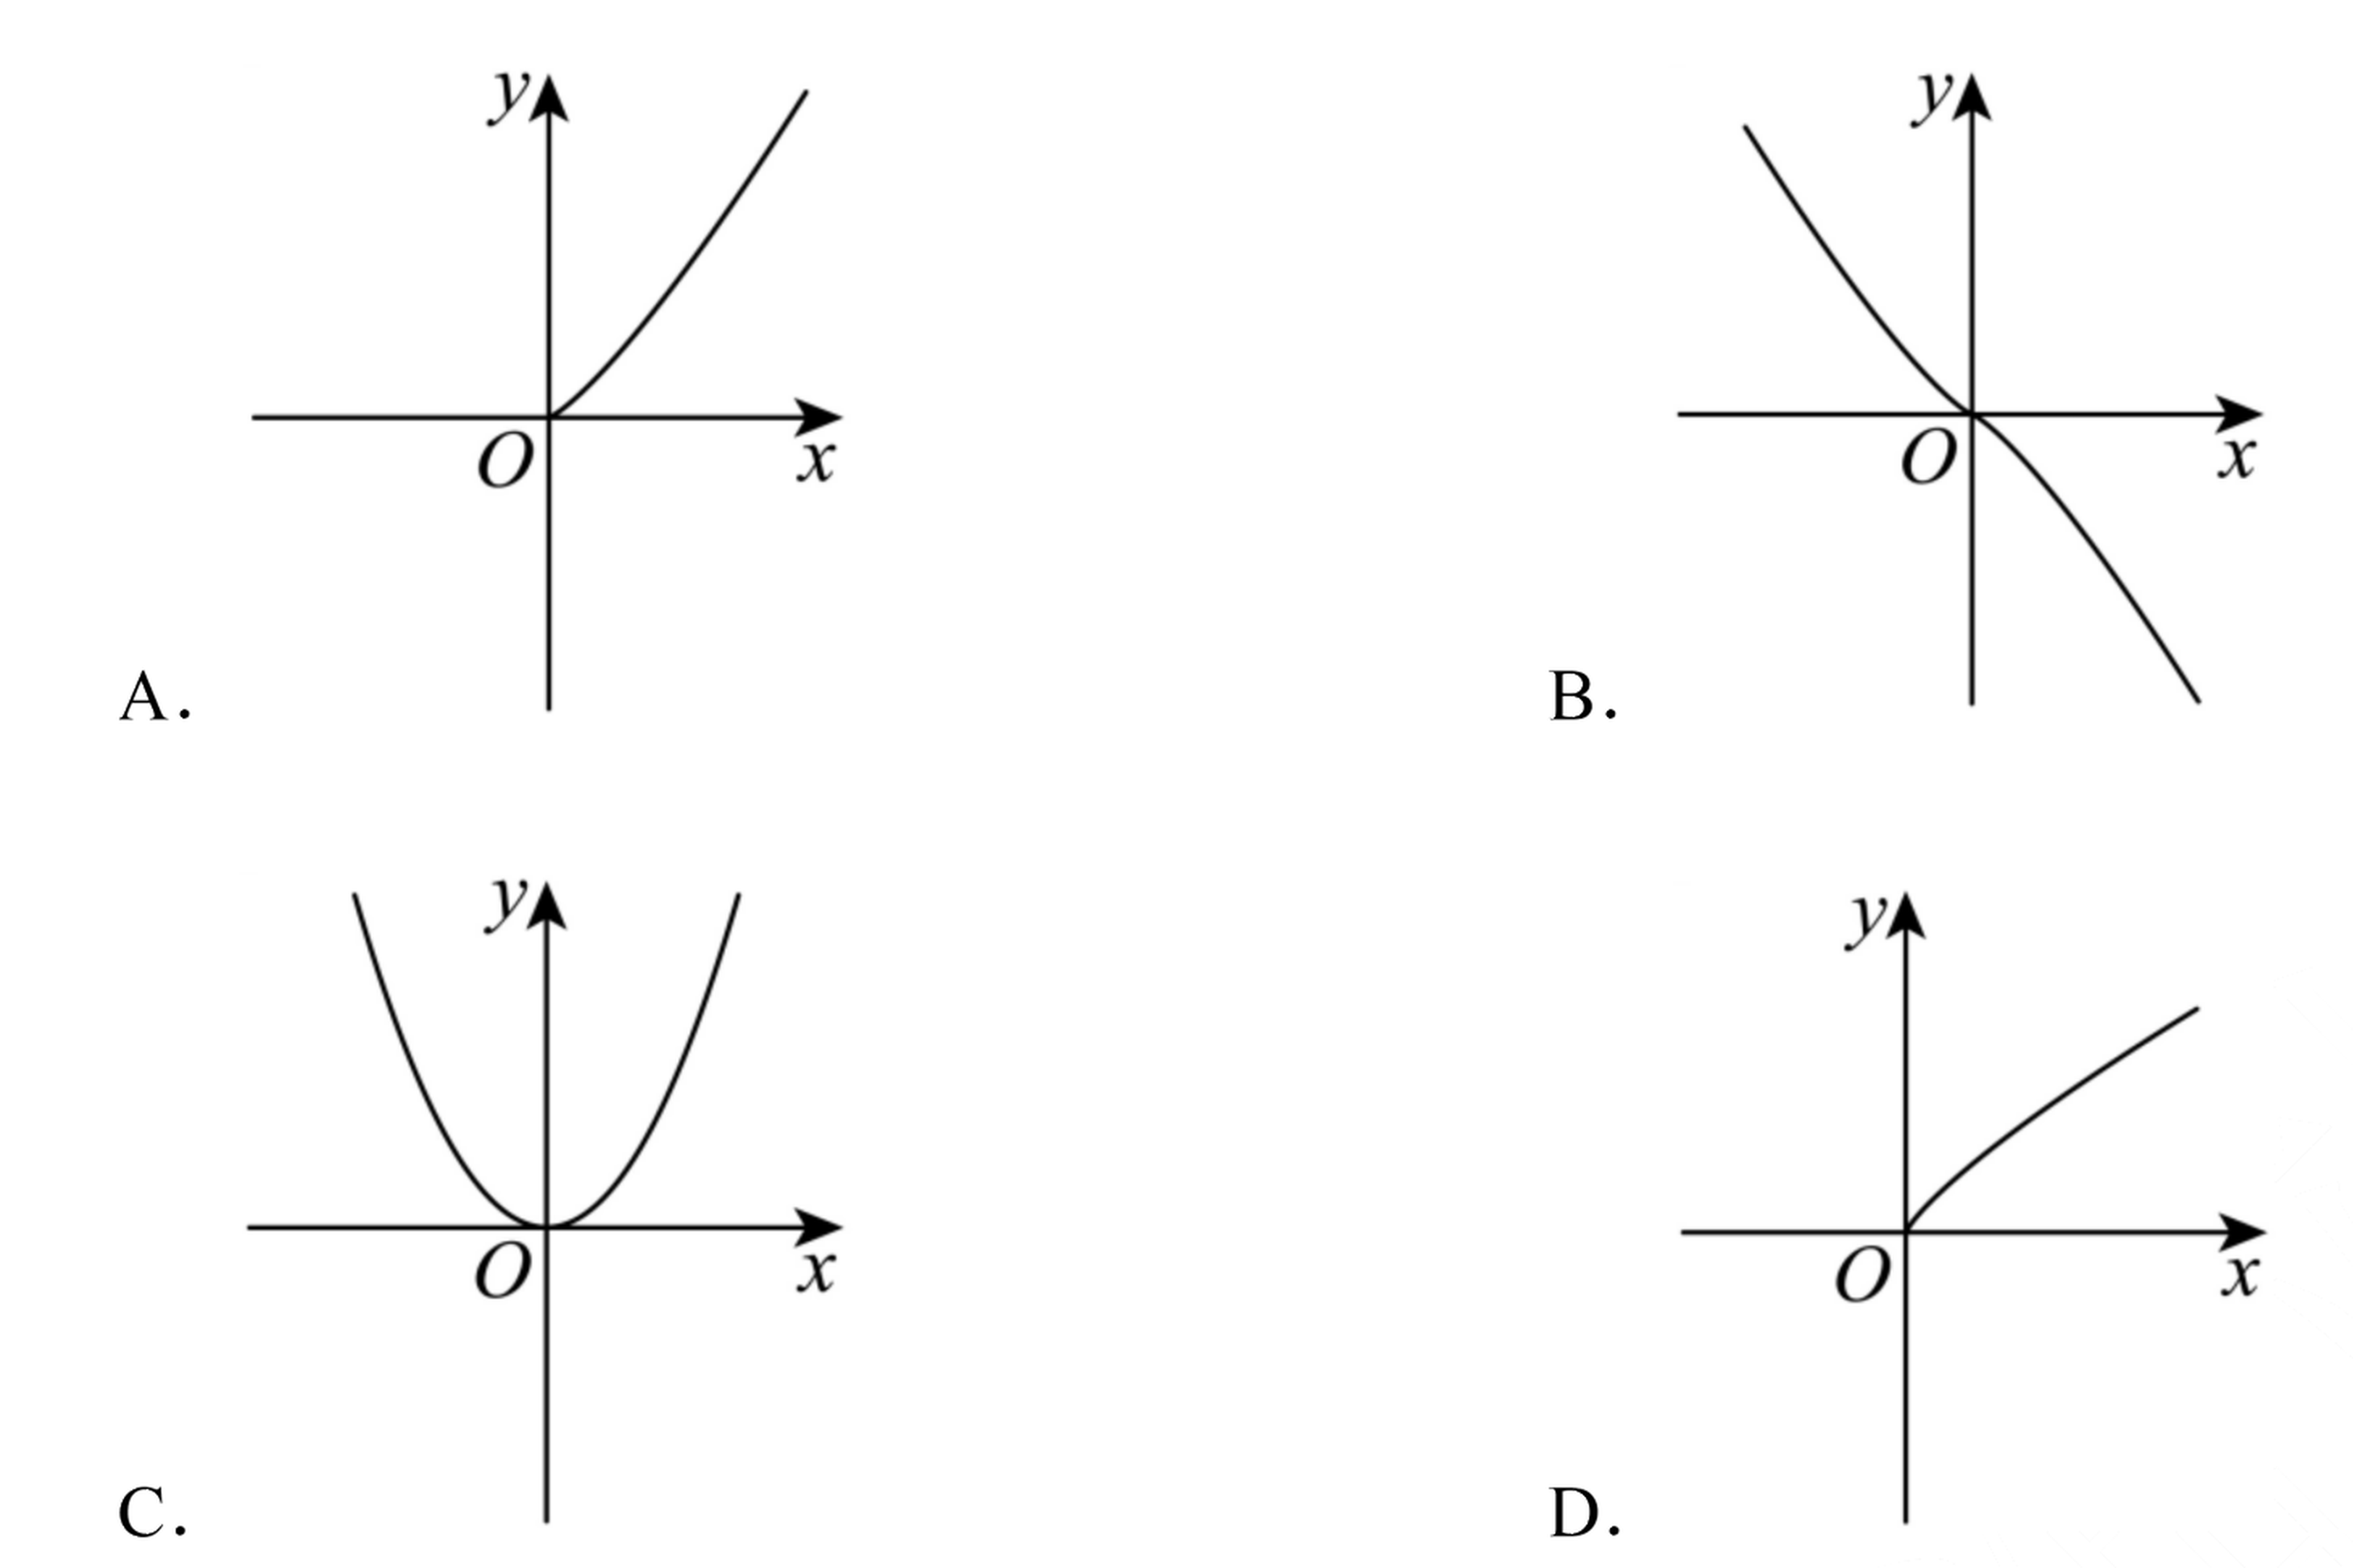
\includegraphics[width=0.80\textwidth]{figures/gao136_q13.png}
\end{center}

\ifanswer
\solbegin
\step{由 $y=x^{\frac54}=\sqrt[4]{x^5}$，函数的定义域为 $[0,+\infty)$，排除 BC，}% 原卷"排除 BC"连写，照录
\step{因为 $\dfrac54>1$，所以函数 $y=x^{\frac54}$ 的图象呈现下凸的趋势，排除 D. 故选 $A$.}
\solend
\fi

\item 下列不等式① $a+\dfrac1a\geqslant2$；② $a^2+4\geqslant4a$；③ $\left\lvert\dfrac ba+\dfrac ab\right\rvert\geqslant2$；④ $\dfrac{2a^2b^2}{a^2+b^2}\leqslant ab$；其中恒成立的是\mbox{（\quad）}

\keepwithprev
A. ①④\qquad B. ③④\qquad C. ②③\qquad D. ①②

\ifanswer
\ans{$C$}
\fi

\item 函数 $y=a^x+b-1(a>0,a\neq1)$ 单调递增且图象不经过第四象限，则 $a,b$ 满足的条件为\mbox{（\quad）}

\keepwithprev
A. $a>1,b\leqslant1$\qquad B. $a>1,b\geqslant0$\qquad C. $0<a<1,b\leqslant1$\qquad D. $0<a<1,b\geqslant1$

\ifanswer
\solbegin
\step{因为函数 $y=a^x+b-1$ 单调递增，所以 $a>1$，}
\step{图象不经过第四象限，则 $x=0$ 时，$y=b\geqslant0$，所以 $a>1,b\geqslant0$，故选 $B$.}
\solend
\fi

\item 设关于 $x$ 的不等式 $\dfrac{ax-1}{x^2-a}<0$ 的解集为 $S$，且 $3\in S$，$4\notin S$，则实数 $a$ 的取值范围为\mbox{（\quad）}

\keepwithprev
A. $(-\infty,-\sqrt3)\cup\left(\dfrac13,\sqrt3\right)$\qquad B. $\left(-\infty,\dfrac14\right)\cup(16,+\infty)$

C. $\left[\dfrac14,\dfrac13\right)\cup(9,16]$\qquad D. 不能确定

\ifanswer
\solbegin
\step{若 $3\in S$，则 $\dfrac{3a-1}{9-a}<0$，解得 $a\in\left(-\infty,\dfrac13\right)\cup(9,+\infty)$，}
\step{若 $4\notin S$，则 $16-a=0$ 或 $\dfrac{4a-1}{16-a}\geqslant0$，解得 $a\in\left[\dfrac14,16\right]$，}
\step{故实数 $a$ 的取值范围为 $\left[\dfrac14,\dfrac13\right)\cup(9,16]$，故选 $C$.}
\solend
\fi

\end{enumerate}

\bigsec{三、解答题}

\begin{enumerate}
\setcounter{enumi}{16}

\item 计算：(1) 计算 $\dfrac{\lg8+\lg125-\lg2-\lg5}{\lg\sqrt{10}\cdot\lg0.1}$；(2) 若 $a^{2x}=2(a>0)$，求 $\dfrac{a^{3x}+a^{-3x}}{a^x+a^{-x}}$.

\ifanswer
\solbegin
\step{(1) 原式 $=\dfrac{2-1}{\frac12\cdot(-1)}=-2$；(2) 原式 $=a^{2x}-1+a^{-2x}=2-1+\dfrac12=\dfrac32$.}
\solend
\fi

\item 不等式 $\dfrac{x-1}{x+1}\geqslant0$ 的解集为 $A$，不等式 $(x-a-1)(2a-x)>0(a<1)$ 的解集为 $B$.

(1) 求集合 $A$；

(2) 若 $B\subseteq A$，求实数 $a$ 的取值范围.

\ifanswer
\solbegin
\step{(1) $A=(-\infty,-1)\cup[1,+\infty)$.}
\step{(2) 由 $(x-a-1)(2a-x)>0(a<1)$，得 $(x-a-1)(x-2a)<0(a<1)$，}
\step{因为 $a<1$，所以 $a+1>2a$，所以 $B=(2a,a+1)$，}
\step{因为 $B\subseteq A$，所以 $2a\geqslant1$ 或 $a+1\leqslant-1$，即 $a\geqslant\dfrac12$ 或 $a\leqslant-2$，}
\step{而 $a<1$，所以实数 $a$ 的取值范围 $(-\infty,-2]\cup\left[\dfrac12,1\right)$.}% 原卷"取值范围"后脱"是／为"，照录
\solend
\fi

\item 已知幂函数 $y=x^m(m\in\R)$ 经过点 $\left(4,\dfrac12\right)$.

(1) 求此幂函数的表达式和定义域；

(2) 已知点 $A(a+2,y_1)$，点 $B(3-2a,y_2)(a\in\R)$ 在此幂函数的图像上，且满足 $y_1<y_2$，求实数 $a$ 的取值范围.

\ifanswer
\solbegin
\step{(1) 幂函数 $y=x^m(m\in\R)$ 经过点 $\left(4,\dfrac12\right)$，所以 $4^m=\dfrac12\Rightarrow m=-\dfrac12$，}
\step{所以 $f(x)=x^{-\frac12}$，定义域为 $(0,+\infty)$.}
\step{(2) 由于函数 $f(x)$ 在其定义域 $(0,+\infty)$ 上严格减，}
\step{由 $y_1<y_2$，得 $a+2>3-2a\geqslant0\Rightarrow a\in\left(\dfrac13,\dfrac32\right]$.}
\solend
\fi

% 第 20 题图取 05 页截图（0.42\textwidth、高约 6cm）。试排 \item 前加 7cm 守卫会多出
% 一张只有两行正文的稀疏页，且三版不加守卫时图均与题干、【解析】同页，故不另加守卫
\item 某医药研究所开发一种抗甲流新药，如果成年人按规定的剂量服用，据监测：服药后每毫升血液中的含药量 $y$（微克）与时间 $t$（小时）之间近似满足如图所示的曲线.

(1) 结合图，求 $k$ 与 $a$ 的值；

(2) 写出服药后 $y$ 与 $t$ 之间的函数关系式 $y=f(t)$；

(3) 据进一步测定：每毫升血液中含药量不少于 $0.5$ 微克时治疗疾病有效，求服药一次治疗有效的时间范围？

\begin{center}
% 图取原卷 05 页截图去粉色水印、去色，3x LANCZOS 放大
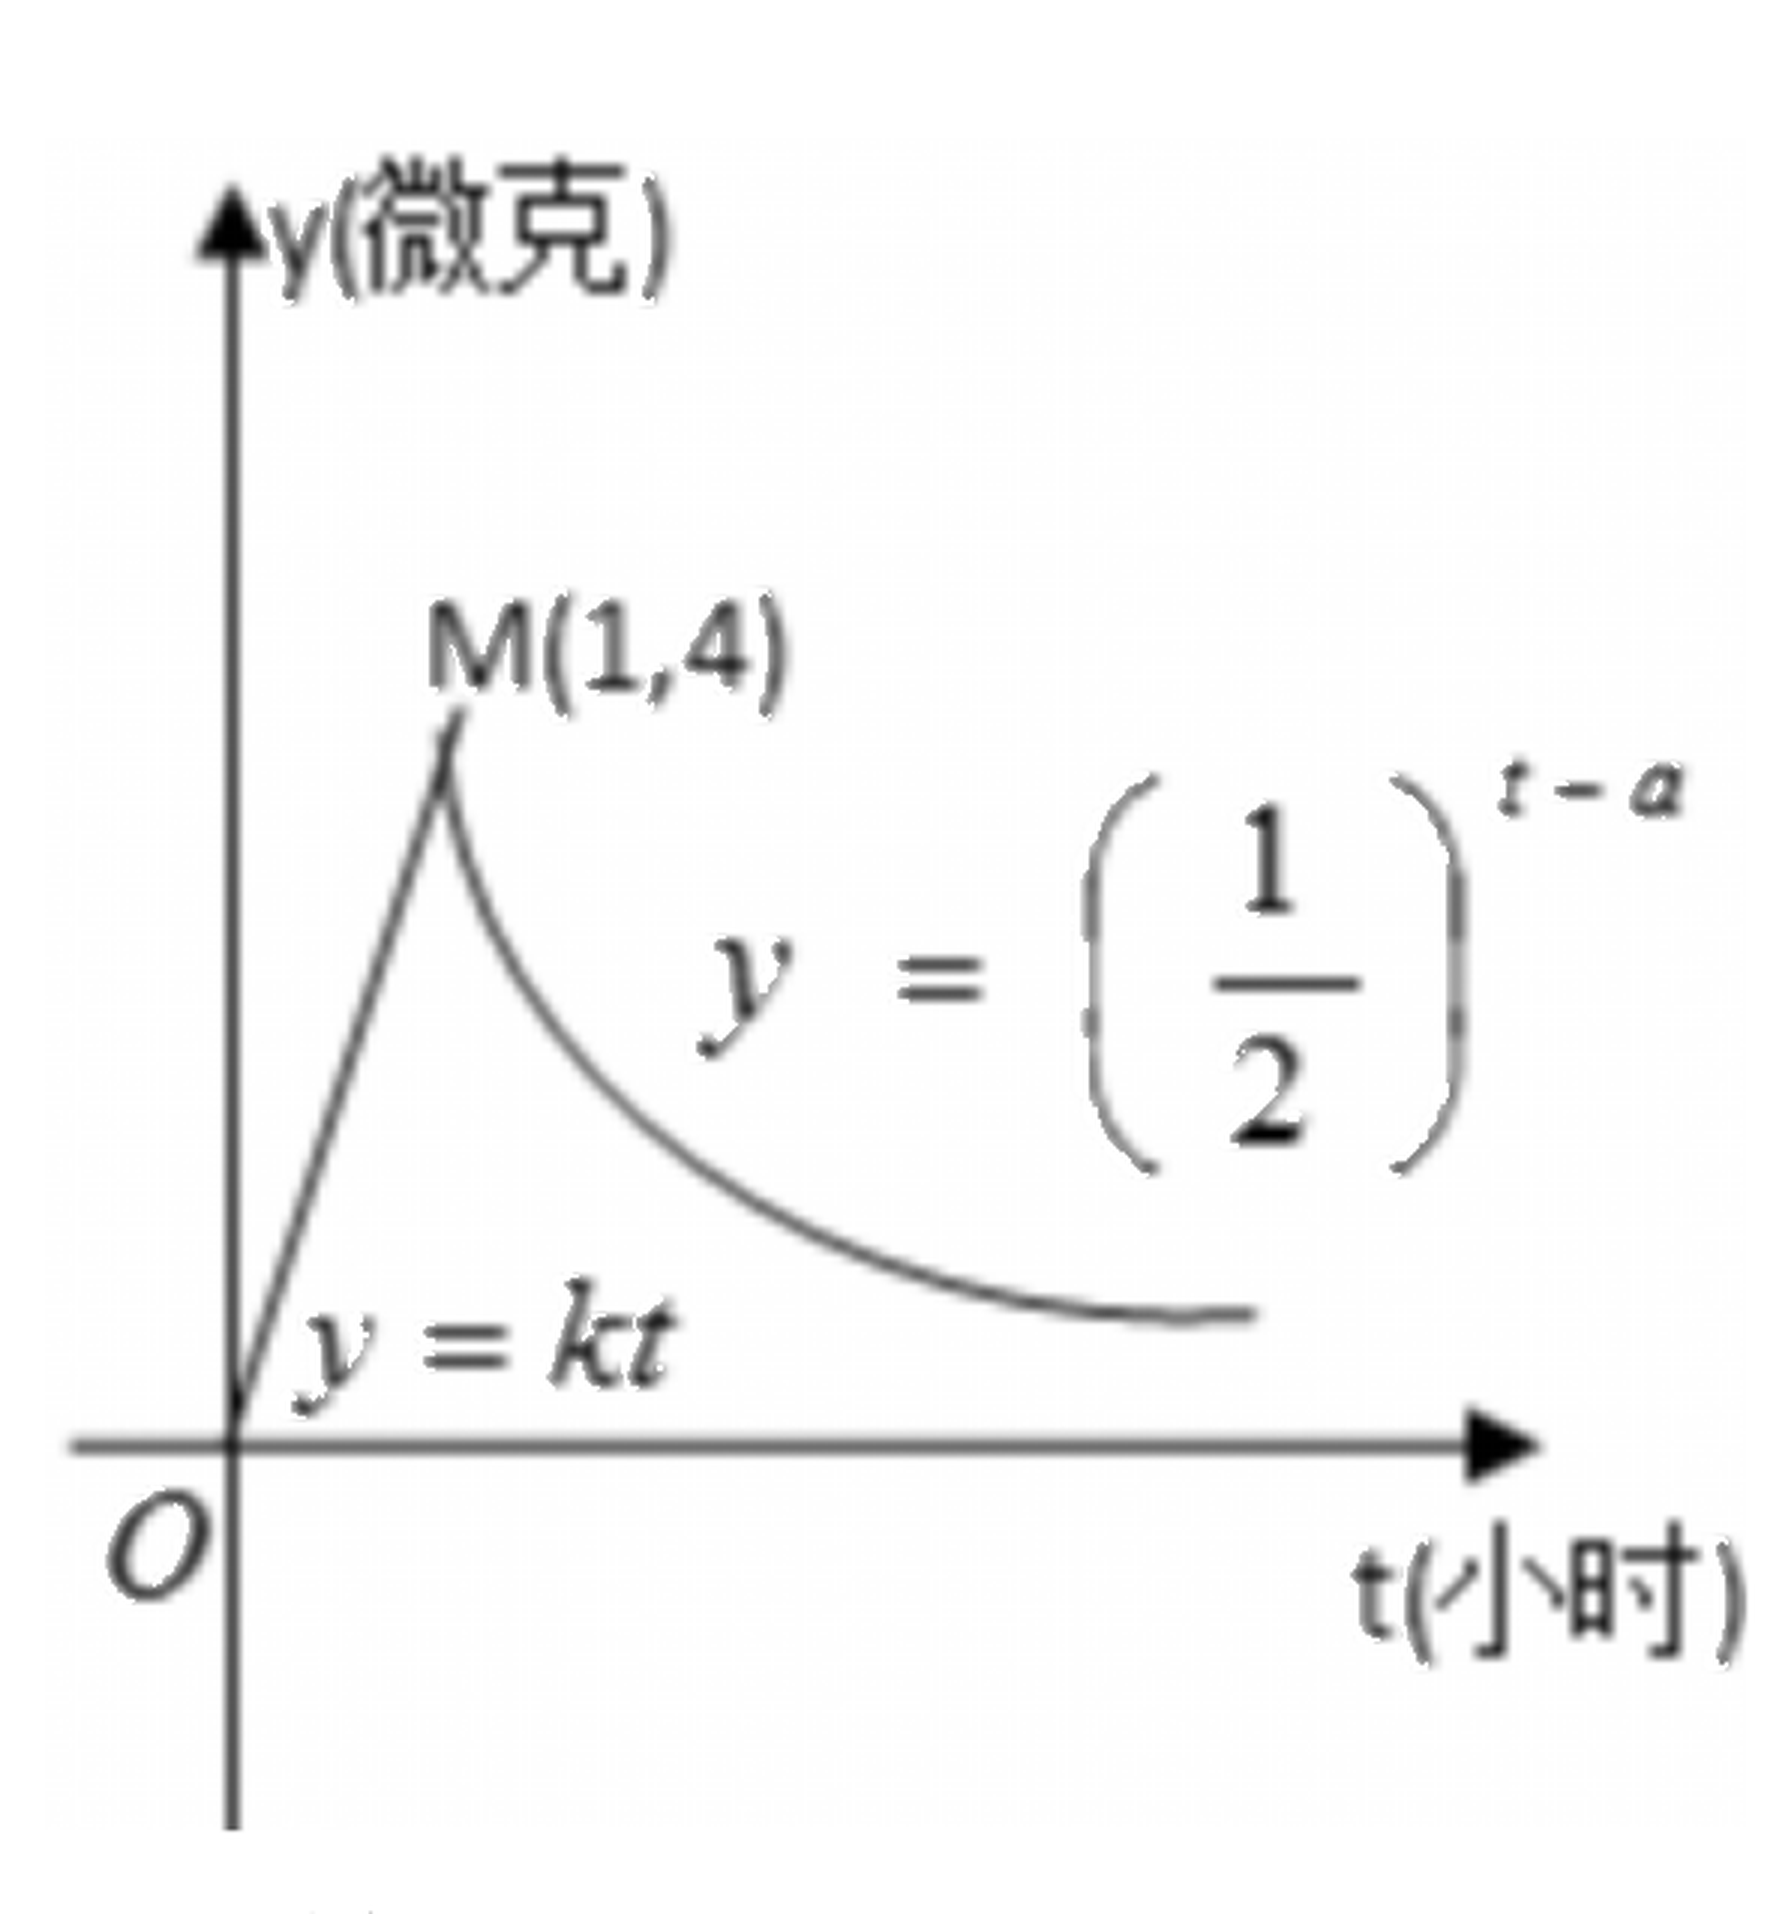
\includegraphics[width=0.42\textwidth]{figures/gao136_q20.png}
\end{center}

\ifanswer
\solbegin
\step{(1) 当 $0\leqslant t\leqslant1$ 时，函数图象是一条线段，由于过原点与点 $(1,4)$，所以 $k=4$，}
\step{其解析式为 $y=4t$，$0\leqslant t\leqslant1$；}
\step{当 $t\geqslant1$ 时，函数的解析式为 $y=\left(\dfrac12\right)^{t-a}$，}
\step{此时 $M(1,4)$ 在曲线上，将此点的坐标代入函数解析式得 $4=\left(\dfrac12\right)^{1-a}$，}
\step{解得 $a=3$；}
\step{(2) 由 (1) 得 $f(t)=\begin{cases}4t,0\leqslant t\leqslant1\\\left(\frac12\right)^{t-3},t>1\end{cases}$；}
\step{(3) 由 (2) 得，令 $f(t)\geqslant0.5$，即 $\begin{cases}4t\geqslant0.5,0\leqslant t\leqslant1\\\left(\frac12\right)^{t-3}\geqslant0.5,t>1\end{cases}$，所以 $\dfrac18\leqslant t\leqslant4$.}
\solend
\fi

\item 已知关于 $x$ 的不等式 $(kx-k^2-4)(x-4)>0$，其中 $k\in\R$.

(1) 当 $k=-1$，求不等式的解集 $A$；

(2) 当 $k$ 变化时，试求不等式的解集 $A$；

(3) 对于不等式解集 $A$，满足 $A\cap\Z=B$. 试探究集合 $B$ 能否为有限集，若能，求出使得集合 $B$ 中元素最少的 $k$ 的所有取值，并用列举法表示此时的集合 $B$，若不能，说明理由；

\ifanswer
\solbegin
\step{(1) 当 $k=-1$ 时，原不等式可化为 $(x+5)(x-4)<0$，}
\step{解得 $-5<x<4$，故不等式的解集为 $\{x\mid -5<x<4\}$；}
\step{(2) 当 $k=0$ 时，解集为 $\{x\mid x<4\}$，}
\step{当 $k>0$ 时，$\dfrac{k^2+4}{k}=k+\dfrac4k\geqslant4$，解集为 $\{x\mid x<4\text{ 或 }x>\dfrac{k^2+4}{k}\}$；}
\step{当 $k<0$ 时，解集为 $\{x\mid \dfrac{k^2+4}{k}<x<4\}$，}
\step{综上，当 $k=0$ 时，$A=\{x\mid x<4\}$，}
\step{当 $k>0$ 时，$A=\{x\mid x<4\text{ 或 }x>\dfrac{k^2+4}{k}\}$；}
\step{当 $k<0$ 时，$A=\{x\mid \dfrac{k^2+4}{k}<x<4\}$，}
\step{(3) 由 (2) 得当 $k\geqslant0$ 时，$B$ 为无限集，当 $k<0$ 时，$B$ 为有限集，}
\step{此时，$\dfrac{k^2+4}{k}=k+\dfrac4k\leqslant-4$，当且仅当 $k=-2$ 时取等号，}
\step{所以 $k=-2$ 时，$B$ 中元素最少，此时 $A=\{x\mid -4<x<4\}$，}
\step{所以 $B=\{-3,-2,-1,0,1,2,3\}$.}
\solend
\fi

\end{enumerate}

% 第 22 题是"四、附加题"首题且带 9cm 图块，守卫须放在 \bigsec 之前连节标题一起量，
% 否则"四、附加题"会孤立在页末（B 类，照 高一26／40／59 成例）
\needvspace{11cm}
\bigsec{四、附加题}

\begin{enumerate}
\setcounter{enumi}{21}

% 第 22 题四幅抛物线/坐标图选项是一整块，守卫放在 \item 之前
\needvspace{9cm}
\item 函数 $f(x)=\left(\dfrac12\right)^{\lvert x+1\rvert}$ 的图象大致为\mbox{（\quad）}

\keepwithprev
\begin{center}
% 四幅抛物线/坐标图选项取原卷 07 页截图去粉色水印，按原卷 2x2 排布合并为一张
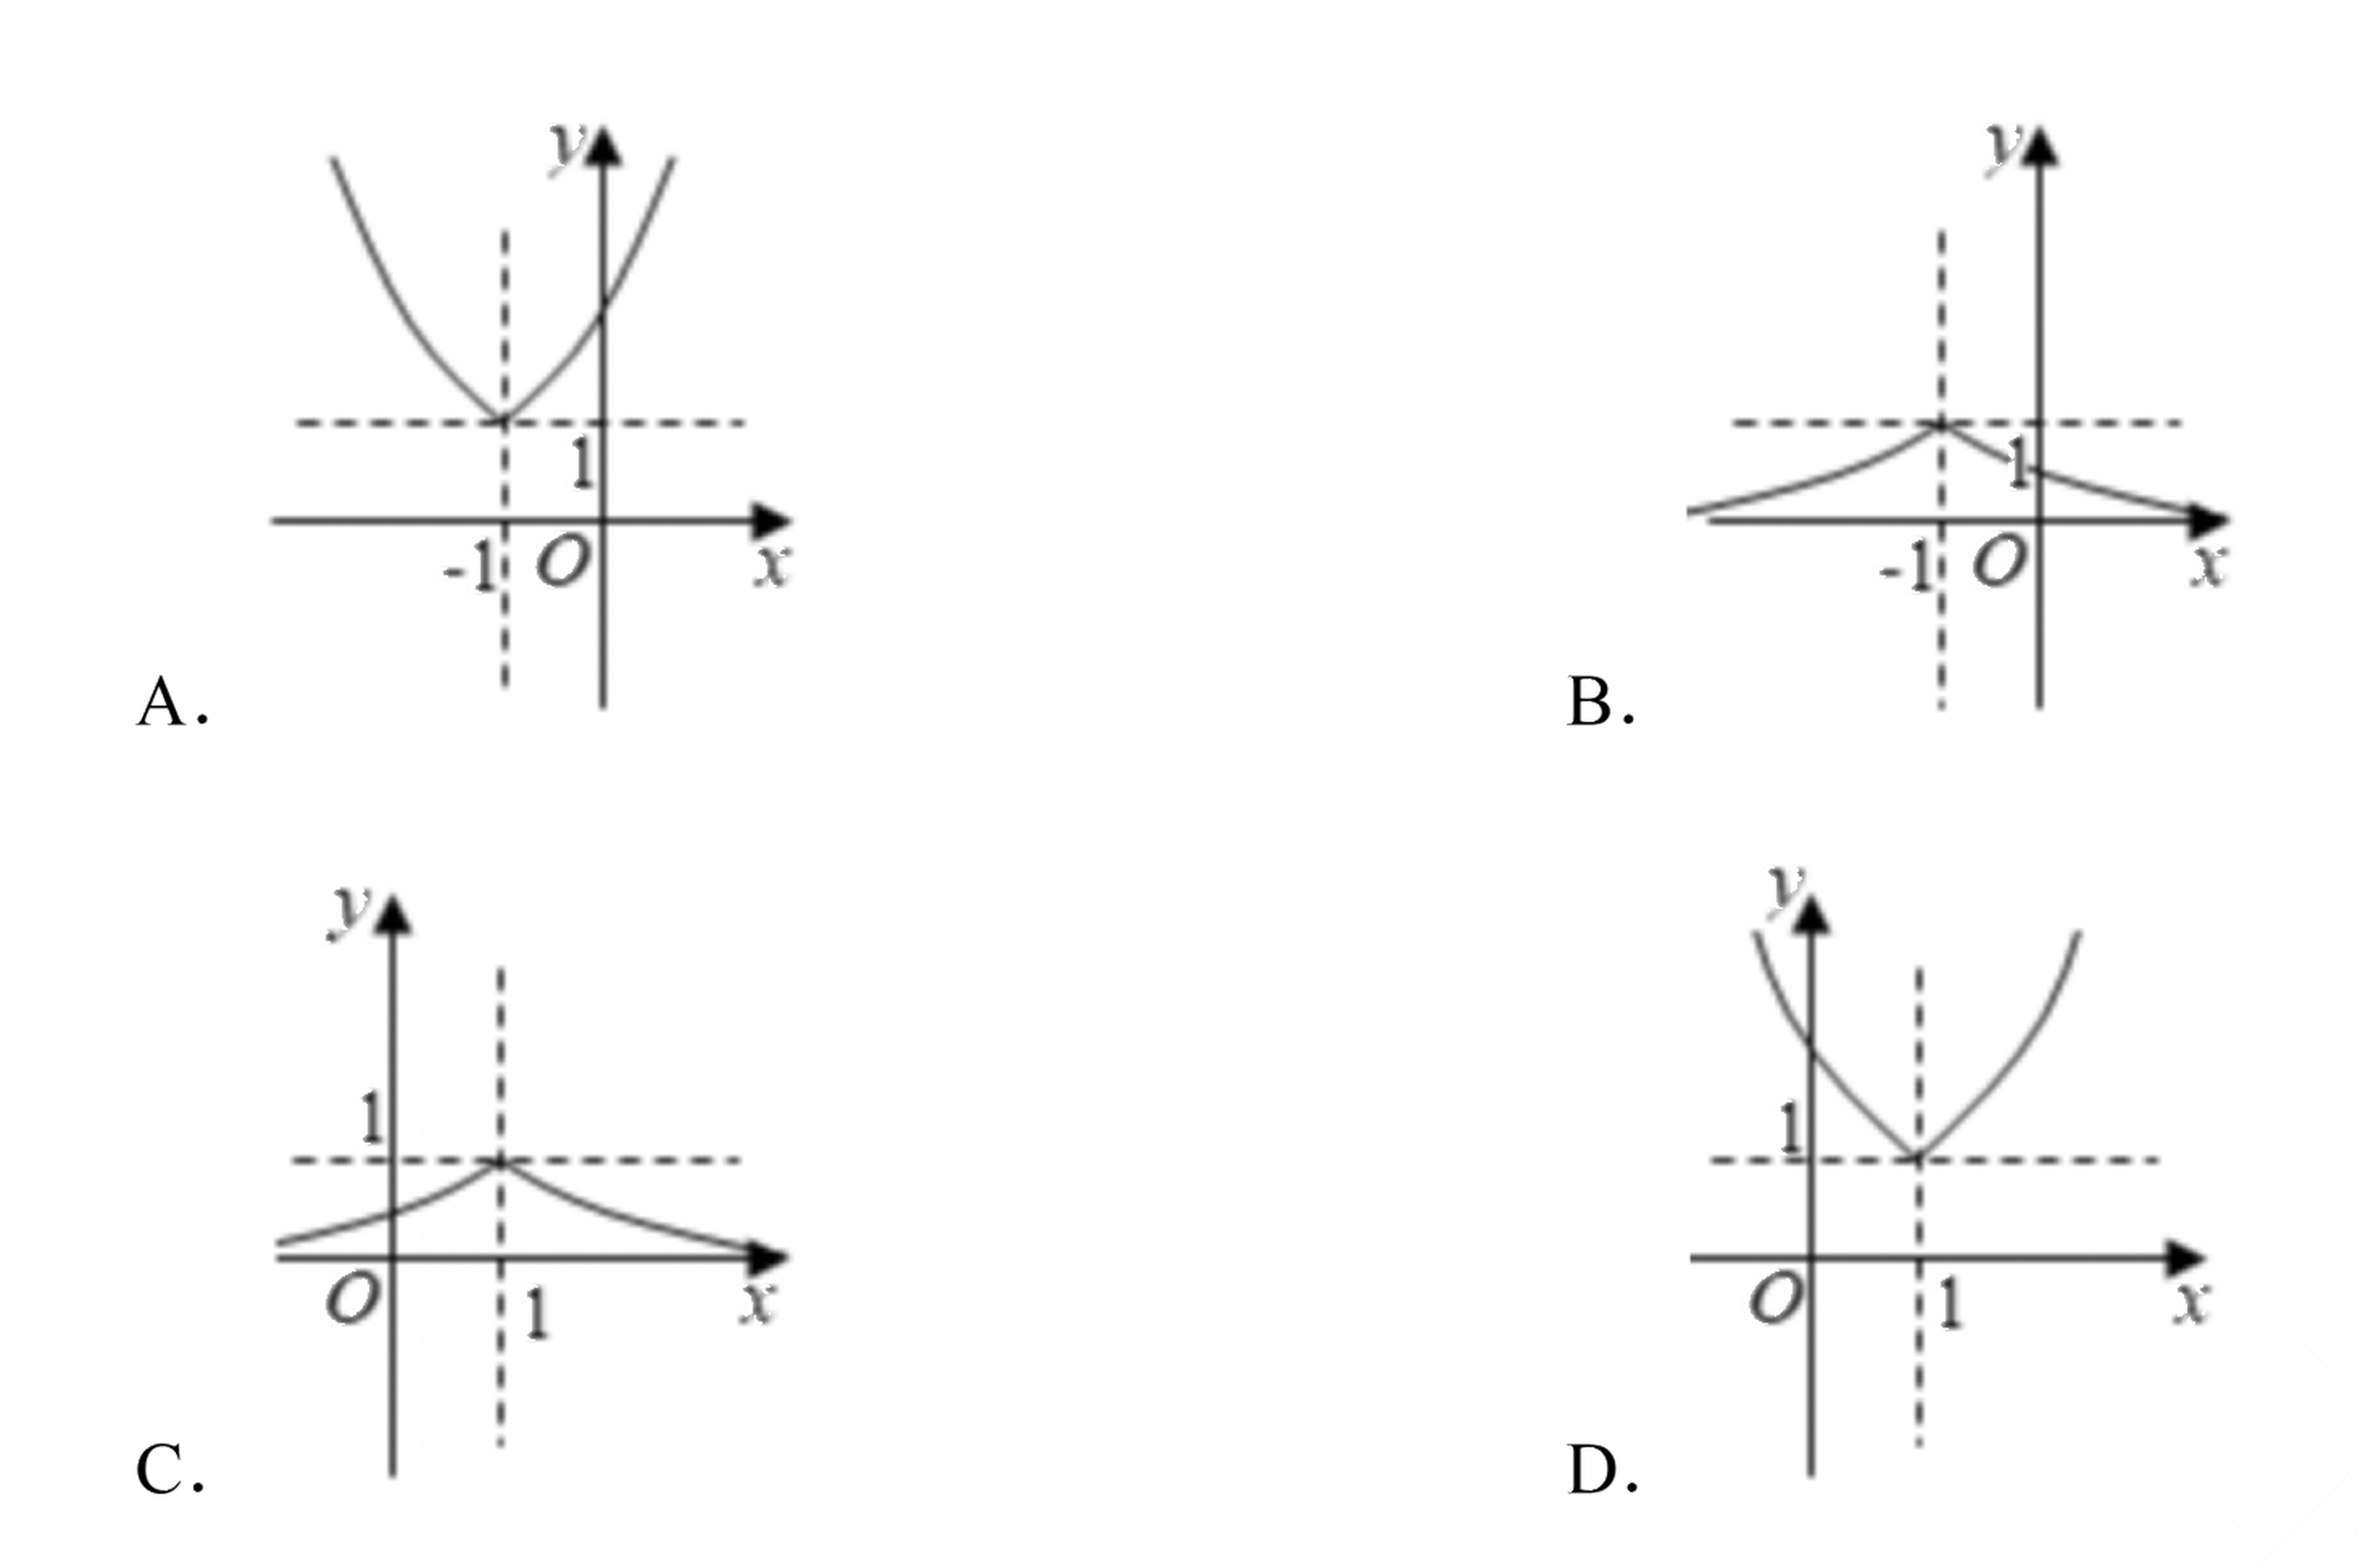
\includegraphics[width=0.80\textwidth]{figures/gao136_q22.png}
\end{center}

\ifanswer
\ans{$B$}
\fi

\end{enumerate}

\end{document}
"
%
% ① 原始材料：微信公众号"魔都数学加油站"文章，作者破晓，2026-11-15 18:04 发布；
% 连载"27学年高一136"，原文标题"27学年高一136——2026-2027年上海市三林中学高一上期中"；
% 原文链接：https://mp.weixin.qq.com/s/jaMzqMm6pDvcT0yM0d7eaQ。
% 正文为 7 张 PNG 页（01、04、06 为 4762x6735；02、03、05、07 为 2560x3620，
% 同一篇各页分辨率不同，逐页按各自分辨率裁图核对），题目下印有【答案】或【解析】，为讲评版。
% 题目、解析均据原图转录；卷面粉红色水印"魔都数学加油站"及公众号页脚未录入。
% 全卷 3 幅插图：第 13 题四幅坐标图选项（03 页）、第 20 题药物浓度折线/曲线图（05 页）、
% 第 22 题四幅抛物线/坐标图选项（07 页），均取原卷截图去粉色水印、去色、LANCZOS 放大，
% 四幅选项按原卷 2x2 排布合并为一张；图前按惯例加 \needvspace 守卫。
%
% 卷首标题：原卷印作"2026-2027 年三林中学高一上期中"（公众号标题中的"上海市"
% 卷面标题行没有，本稿照卷面），年份区间按全稿惯例排 en dash；原卷未印副标题，
% 本卷为期中卷、跨集合与常用逻辑用语／不等式／函数三章，按题目内容标为
% "集合与常用逻辑用语、不等式、函数"（与 125／126／128／129／131／132／133 同期中卷口径相同）：
% 集合与逻辑见 Q3、Q6、Q10、Q12、Q16、Q18、Q21，不等式见 Q5、Q7、Q8、Q9、Q14、Q15，
% 函数（幂函数、指数／对数、基本不等式应用）见 Q4、Q11、Q13、Q17、Q19、Q20、Q22。
%
% 题号体例：本卷共 20 题——一、填空题 3—12（10 题）、二、选择题 13—16（4 题）、
% 三、解答题 17—21（5 题）、四、附加题 22（1 题）。四节分别
% \setcounter{enumi}{2}／{12}／{16}／{21}。
%
% ② 与原卷的排版差异：
%   ① 原文从第 3 题起，本稿保留原题号；末节"四、附加题"另起 \bigsec，题号续到 22；
%   ② 原卷每题下直接印【答案】或【解析】，本稿按全稿惯例置于答案版；第 3、4、6 题只印
%      【答案】、无【解析】，提 \ans{}；第 14 题答案 C 印在题干括号内、无【解析】，按
%      高一53／高一108／高一132／高一133 成例括号留空、另提 \ans{$C$}；第 22 题答案 B
%      印在题干括号内、无【解析】，同例提 \ans{$B$}；第 13、15、16 题答案在解析末句
%      "故选 …"，括号内留空、不另提 \ans{}；其余各题印【解析】、无独立答案段；
%   ③ 原卷未印副标题，本稿按"知识模块"口径补出；
%   ④ 原卷填空横线按全稿惯例排为 \blankline[4.4em]；选择题括号排 \mbox{（\quad）}、
%      每个选项段前按惯例加 \keepwithprev（四幅图选项那一枚放在 \begin{center} 之前）；
%      解答题不留作答区、不加 \anspace（原卷为讲评版，与 129／131／132／133 同）；
%   ⑤ 原卷数集排斜体 $R$／$R^+$／$Z$，按全稿惯例改 \R／\R^+／\Z；空集记号 \varnothing；
%      绝对值排 \lvert…\rvert，集合描述竖线排 \mid；不等号按全稿惯例排 \leqslant／\geqslant；
%   ⑥ 子题标号 (1)(2)(3) 原卷用半角括号，照录；圈数字 ①②③④ 照录；第 12 题甲／乙／丙
%      三行与第 14 题四个编号不等式照录；
%   ⑦ 数学式内半角逗号照录（如 Q4"$a>0,a\neq1$"、Q6"$\{(-2,4),(1,1)\}$"、
%      Q7"$a=2+3=5,b=2\times3=6$"、Q11"$x_1,x_2$"、Q12"$m,n\in R^+$"、
%      Q15"$a>1,b\geq0$"、Q18"$B=(2a,a+1)$"、Q20"$4t,0\leq t\leq1$"、
%      Q21"$\{-3,-2,-1,0,1,2,3\}$"）；原卷行末西文句点照录，行中全角逗号照录；
%   ⑧ 三幅插图：第 13 题四幅坐标图选项合并裁为一张 \includegraphics（题前 \needvspace{9cm}）；
%      第 20 题折线/曲线图取 05 页截图（0.42\textwidth）；第 22 题四幅抛物线/坐标图选项合并
%      裁为一张（题前 \needvspace{9cm}）。第 13、22 题分别是"二、选择题""四、附加题"的首题
%      且带大图块，另在两处 \bigsec 之前各加 \needvspace{11cm} 连节标题一起量，避免节标题
%      孤立在页末（切页审计 B 类；照 高一26／40／59 成例）。第 20 题图不是节首题、三版试排
%      图均与题干同页，加 7cm 守卫反会多出一张只有两行正文的稀疏页，故不另加守卫；
%      三版切页审计均"合计异常：无"（试卷 4 页／紧凑 4 页／答案 6 页）；
%   ⑨ 跨页续印按题合并：Q16 题干在 03 页、括号与选项及【解析】在 04 页；Q19 题干在 04 页、
%      (2) 与【解析】在 05 页；Q20 (3)【解析】在 06 页；Q22 四幅图在 07 页；本稿按题连排；
%   ⑩ 题干中的中文弯引号按原卷照录，注释内一律 ASCII 引号；原卷"图像／图象"两种写法混用，
%      逐处照录（Q4、Q19 作"图像"，Q13、Q15、Q20、Q22 作"图象"）；
%   ⑪ 附加题节：原卷印"四、附加题"，本稿用 \bigsec{四、附加题} 另起一节、
%      \setcounter{enumi}{21}，顶层 1 个 \item（与 高一09／15／16／22／35／39／47／61 同口径）；
%      Q22 只印括号内答案、提 \ans{}，不计入 \step 账。
%
% 判别式字形：全卷仅第 9 题【解析】cases 块出现判别式"$\Delta=a^2-8a<0$"，原卷印
%   等腰、偏高的三角 $\Delta$，逐处放大核对并照录 \Delta；全卷未出现扁等边三角 \triangle。
%
% 子集符号：第 18 题 (2) 题干"$B\subseteq A$"与【解析】"$B\subseteq A$"两处原卷均印
%   带下划线 $\subseteq$，逐处放大核对、照录 \subseteq；全卷未出现单线 \subset。
%
% 原卷存疑照录（均照录未改，正文对应处另有 % 注）：
%   第 12 题乙行"$\dfrac{m+n}{mm}=\dfrac1{mn}$"前一分母印作 $mm$（后一处作 $mn$），照录；
%   第 12 题【解析】"$\geqslant\dfrac1{100}\left[a^2+1+2\sqrt{a^2}\right]$"保留 $\sqrt{a^2}$
%      未化简为 $a$，照录；
%   第 13 题【解析】"排除 BC"与"排除 D"连写选项字母，照录；
%   第 18 题 (2)【解析】末行"所以实数 $a$ 的取值范围 $(-\infty,-2]\cup[\frac12,1)$"
%      "取值范围"后脱"是／为"字，照录；
%   第 21 题 (3) 题干"求出使得集合 $B$ 中元素最少的 $k$ 的所有取值"而【解析】只给出
%      $k=-2$ 一处，措辞照录。
%
% 行数复核：逐题数 \step 条数，合计 51 条（Q3：0；Q4：0；Q5：2；Q6：0；Q7：2；Q8：1；
% Q9：1；Q10：4；Q11：1；Q12：4；Q13：2；Q14：0；Q15：2；Q16：3；Q17：1；Q18：5；
% Q19：4；Q20：7；Q21：12；Q22：0），与原卷印刷行逐题相等（cases 块作一个印刷行计）。
% 第 3、4、6、14、22 题只印【答案】、提 \ans{}，不计入 \step 账；第 13、15、16 题答案在
% 解析末句，括号内留空、不另提 \ans{}。
%
\documentclass[a4paper,11pt]{article}
\usepackage{common}

\begin{document}

\examtitlest[3]{2026--2027 年三林中学高一上期中}{集合与常用逻辑用语、不等式、函数}

\bigsec{一、填空题}

\begin{enumerate}
\setcounter{enumi}{2}

\item 用反证法证明命题“若 $x+y\neq5$，则 $x\neq2$ 或 $y\neq3$”为真命题时，第一个步骤是\blankline[4.4em].

\ifanswer
\ans{假设 $x=2$ 且 $y=3$}
\fi

\item 函数 $y=a^{x-1}+1(a>0,a\neq1)$ 的图像恒过定点 $A$，则点的坐标是\blankline[4.4em].

\ifanswer
\ans{$(1,2)$}
\fi

\item 已知 $x>1$，则 $x+\dfrac4{x-1}$ 的最小值是\blankline[4.4em].

\ifanswer
\solbegin
\step{由 $x>1$，得 $x-1>0$，则 $x+\dfrac4{x-1}=x-1+\dfrac4{x-1}+1\geqslant2\sqrt{(x-1)\cdot\dfrac4{x-1}}+1=5$，}
\step{当且仅当 $x-1=\dfrac4{x-1}$ 即 $x=3$ 时取等号，取得最小值 $5$.}
\solend
\fi

\item 已知集合 $A=\{(x,y)\mid y=x^2\}$，集合 $B=\{(x,y)\mid y=2-x\}$，求 $A\cap B=$\blankline[4.4em].

\ifanswer
\ans{$\{(-2,4),(1,1)\}$}
\fi

\item 已知一元二次不等式 $x^2-ax+b<0$ 的解集为 $(2,3)$，则不等式 $bx^2-ax+1>0$ 的解集是\blankline[4.4em].

\ifanswer
\solbegin
\step{$a=2+3=5,b=2\times3=6$，则 $bx^2-ax+1>0$ 即 $6x^2-5x+1>0$，}
\step{即 $(3x-1)(2x-1)>0$，解集为 $\left(-\infty,\dfrac13\right)\cup\left(\dfrac12,+\infty\right)$.}
\solend
\fi

\item 不等式 $(x+2)^3<(5-2x)^3$ 的解集为\blankline[4.4em].

\ifanswer
\solbegin
\step{由 $(x+2)^3<(5-2x)^3$ 得 $x+2<5-2x$，故解集为 $(-\infty,1)$.}
\solend
\fi

\item 若关于 $x$ 的不等式 $ax^2-ax+2>0$ 的解集为 $\R$，则实数 $a$ 的取值范围是\blankline[4.4em].

\ifanswer
\solbegin
\step{由题意得 $a=0$ 或 $\begin{cases}a>0\\\Delta=a^2-8a<0\end{cases}$，所以 $0\leqslant a<8$.}% 判别式原卷印高三角 $\Delta$，照录
\solend
\fi

\item 已知关于 $x$ 的不等式 $\lvert x+3\rvert+\lvert x-a\rvert\geqslant5$ 恒成立，则实数 $a$ 的取值范围为\blankline[4.4em].

\ifanswer
\solbegin
\step{因为 $\lvert x+3\rvert+\lvert x-a\rvert\geqslant\lvert x-a-x-3\rvert=\lvert 3+a\rvert$，}
\step{要使 $\lvert x+3\rvert+\lvert x-a\rvert\geqslant5$ 恒成立，则 $\lvert a+3\rvert\geqslant5$ 即可，}
\step{所以 $a+3\geqslant5$ 或 $a+3\leqslant-5$，解得 $a\geqslant2$ 或 $a\leqslant-8$，}
\step{即实数 $a$ 的取值范围是 $(-\infty,-8]\cup[2,+\infty)$.}
\solend
\fi

\item 若方程 $\lg^2 x-2\lg x-2=0$ 的两个解为 $x_1,x_2$，求 $\log_{x_1}x_2+\log_{x_2}x_1$ 的值为\blankline[4.4em].

\ifanswer
\solbegin
\step{$\log_{x_1}x_2+\log_{x_2}x_1=\dfrac{\lg x_2}{\lg x_1}+\dfrac{\lg x_1}{\lg x_2}=\dfrac{(\lg x_1+\lg x_2)^2-2\lg x_1\lg x_2}{\lg x_1\lg x_2}=-4$.}
\solend
\fi

\item 三个同学对问题“已知 $m,n\in \R^+$，且 $m+n=1$，求 $\dfrac1m+\dfrac1n$ 的最小值”提出各自的解题思路：

思路：

甲：$\dfrac1m+\dfrac1n=\dfrac{m+n}{m}+\dfrac{m+n}{n}=2+\dfrac nm+\dfrac mn$，可用基本不等式求解；

乙：$\dfrac1m+\dfrac1n=\dfrac{m+n}{mm}=\dfrac1{mn}=\dfrac1{m(1-m)}$，可用二次函数配方法求解；% 原卷前一分母印作 $mm$，照录

丙：$\dfrac1m+\dfrac1n=\left(\dfrac1m+\dfrac1n\right)(m+n)=2+\dfrac nm+\dfrac mn$，可用基本不等式求解；参考上述解题思路，

可求得当 $x=$\blankline[4.4em]时，$y=\dfrac{a^2}{x^2}+\dfrac1{100-x^2}$（$0<x<10$，$a>0$）有最小值.

\ifanswer
\solbegin
\step{$y=\dfrac{a^2}{x^2}+\dfrac1{100-x^2}=\left(\dfrac{a^2}{x^2}+\dfrac1{100-x^2}\right)[x^2+(100-x^2)]\times\dfrac1{100}$}
\step{$=\dfrac1{100}\left[a^2+1+\dfrac{x^2}{100-x^2}+\dfrac{a^2(100-x^2)}{x^2}\right]\geqslant\dfrac1{100}\left[a^2+1+2\sqrt{a^2}\right]$}% 原卷保留 $\sqrt{a^2}$ 未化简，照录
\step{当且仅当 $\dfrac{x^2}{100-x^2}=\dfrac{a^2(100-x^2)}{x^2}$，即 $x=\sqrt{\dfrac{100a}{a+1}}$ 时，}
\step{$y=\dfrac{a^2}{x^2}+\dfrac1{100-x^2}(0<x<10,a>0)$ 有最小值.}
\solend
\fi

\end{enumerate}

% 第 13 题是"二、选择题"首题且带 9cm 图块，守卫须放在 \bigsec 之前连节标题一起量，
% 否则"二、选择题"会孤立在页末（B 类，照 高一26／40／59 成例）
\needvspace{11cm}
\bigsec{二、选择题}

\begin{enumerate}
\setcounter{enumi}{12}

% 第 13 题四幅坐标图选项是一整块，守卫放在 \item 之前
\needvspace{9cm}
\item 下列图象中，最符合函数 $y=x^{\frac54}$ 的图象的是\mbox{（\quad）}

\keepwithprev
\begin{center}
% 四幅坐标图选项取原卷 03 页截图去粉色水印，按原卷 2x2 排布合并为一张
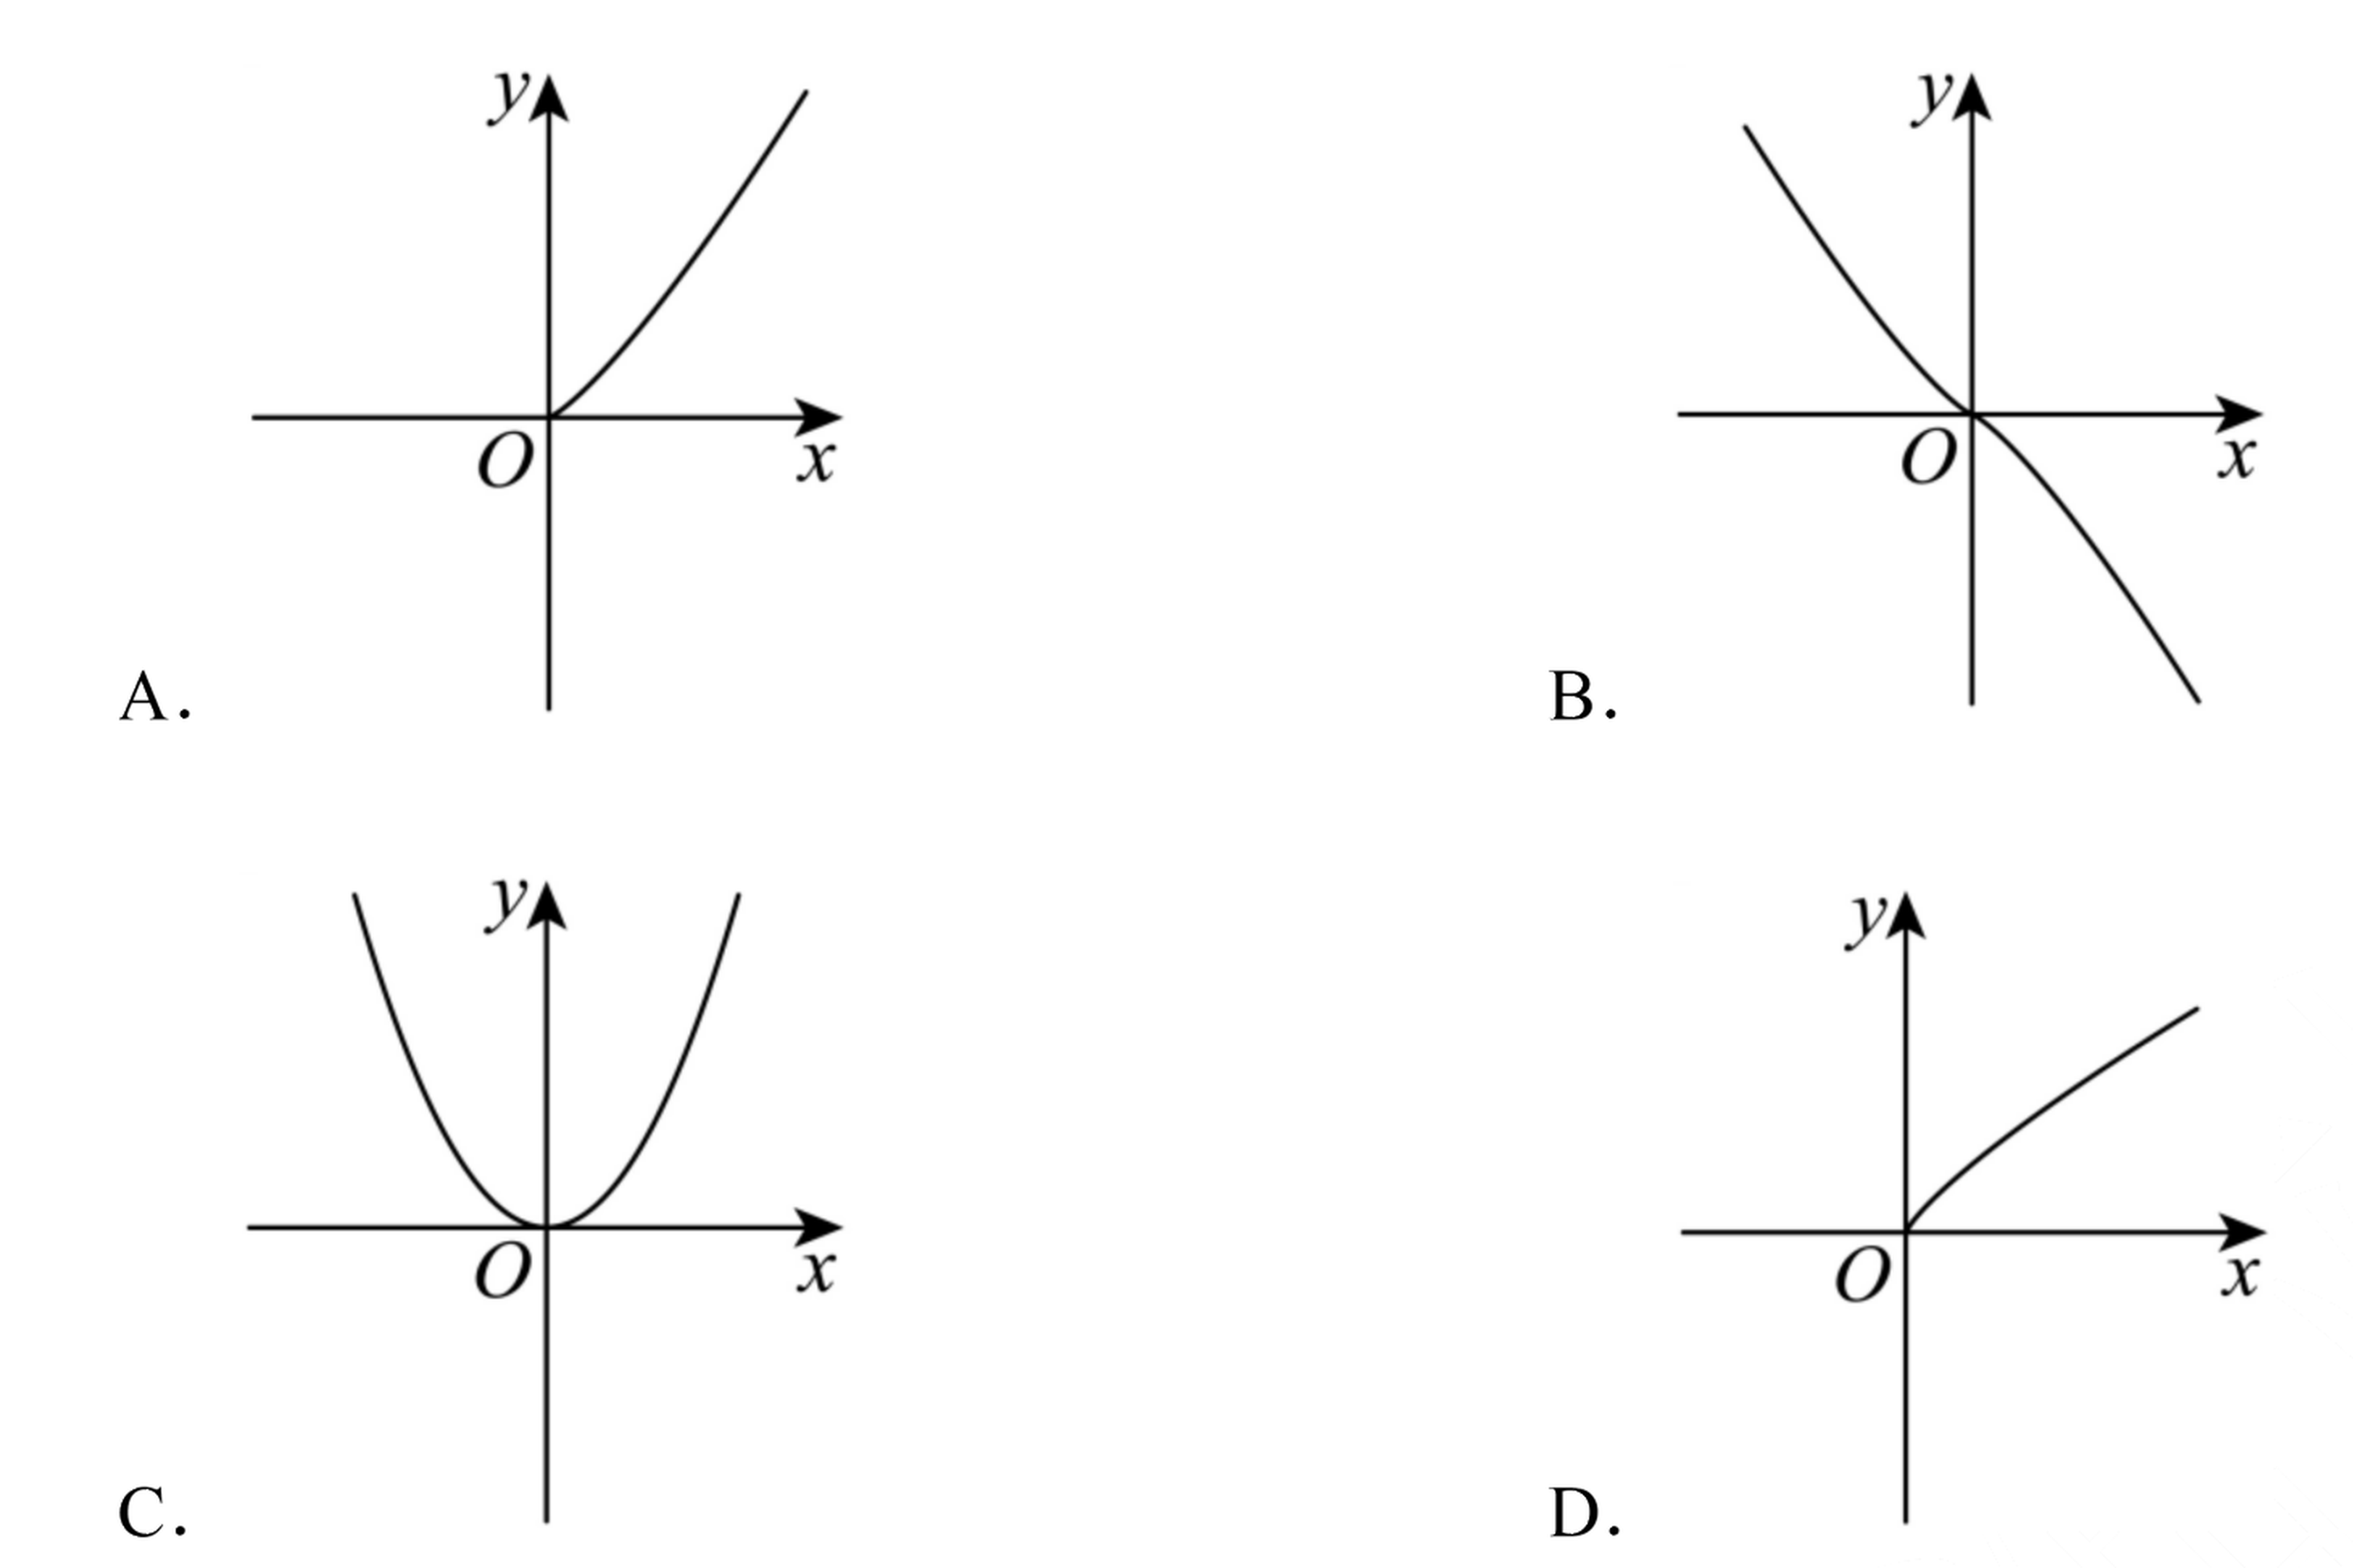
\includegraphics[width=0.80\textwidth]{figures/gao136_q13.png}
\end{center}

\ifanswer
\solbegin
\step{由 $y=x^{\frac54}=\sqrt[4]{x^5}$，函数的定义域为 $[0,+\infty)$，排除 BC，}% 原卷"排除 BC"连写，照录
\step{因为 $\dfrac54>1$，所以函数 $y=x^{\frac54}$ 的图象呈现下凸的趋势，排除 D. 故选 $A$.}
\solend
\fi

\item 下列不等式① $a+\dfrac1a\geqslant2$；② $a^2+4\geqslant4a$；③ $\left\lvert\dfrac ba+\dfrac ab\right\rvert\geqslant2$；④ $\dfrac{2a^2b^2}{a^2+b^2}\leqslant ab$；其中恒成立的是\mbox{（\quad）}

\keepwithprev
A. ①④\qquad B. ③④\qquad C. ②③\qquad D. ①②

\ifanswer
\ans{$C$}
\fi

\item 函数 $y=a^x+b-1(a>0,a\neq1)$ 单调递增且图象不经过第四象限，则 $a,b$ 满足的条件为\mbox{（\quad）}

\keepwithprev
A. $a>1,b\leqslant1$\qquad B. $a>1,b\geqslant0$\qquad C. $0<a<1,b\leqslant1$\qquad D. $0<a<1,b\geqslant1$

\ifanswer
\solbegin
\step{因为函数 $y=a^x+b-1$ 单调递增，所以 $a>1$，}
\step{图象不经过第四象限，则 $x=0$ 时，$y=b\geqslant0$，所以 $a>1,b\geqslant0$，故选 $B$.}
\solend
\fi

\item 设关于 $x$ 的不等式 $\dfrac{ax-1}{x^2-a}<0$ 的解集为 $S$，且 $3\in S$，$4\notin S$，则实数 $a$ 的取值范围为\mbox{（\quad）}

\keepwithprev
A. $(-\infty,-\sqrt3)\cup\left(\dfrac13,\sqrt3\right)$\qquad B. $\left(-\infty,\dfrac14\right)\cup(16,+\infty)$

C. $\left[\dfrac14,\dfrac13\right)\cup(9,16]$\qquad D. 不能确定

\ifanswer
\solbegin
\step{若 $3\in S$，则 $\dfrac{3a-1}{9-a}<0$，解得 $a\in\left(-\infty,\dfrac13\right)\cup(9,+\infty)$，}
\step{若 $4\notin S$，则 $16-a=0$ 或 $\dfrac{4a-1}{16-a}\geqslant0$，解得 $a\in\left[\dfrac14,16\right]$，}
\step{故实数 $a$ 的取值范围为 $\left[\dfrac14,\dfrac13\right)\cup(9,16]$，故选 $C$.}
\solend
\fi

\end{enumerate}

\bigsec{三、解答题}

\begin{enumerate}
\setcounter{enumi}{16}

\item 计算：(1) 计算 $\dfrac{\lg8+\lg125-\lg2-\lg5}{\lg\sqrt{10}\cdot\lg0.1}$；(2) 若 $a^{2x}=2(a>0)$，求 $\dfrac{a^{3x}+a^{-3x}}{a^x+a^{-x}}$.

\ifanswer
\solbegin
\step{(1) 原式 $=\dfrac{2-1}{\frac12\cdot(-1)}=-2$；(2) 原式 $=a^{2x}-1+a^{-2x}=2-1+\dfrac12=\dfrac32$.}
\solend
\fi

\item 不等式 $\dfrac{x-1}{x+1}\geqslant0$ 的解集为 $A$，不等式 $(x-a-1)(2a-x)>0(a<1)$ 的解集为 $B$.

(1) 求集合 $A$；

(2) 若 $B\subseteq A$，求实数 $a$ 的取值范围.

\ifanswer
\solbegin
\step{(1) $A=(-\infty,-1)\cup[1,+\infty)$.}
\step{(2) 由 $(x-a-1)(2a-x)>0(a<1)$，得 $(x-a-1)(x-2a)<0(a<1)$，}
\step{因为 $a<1$，所以 $a+1>2a$，所以 $B=(2a,a+1)$，}
\step{因为 $B\subseteq A$，所以 $2a\geqslant1$ 或 $a+1\leqslant-1$，即 $a\geqslant\dfrac12$ 或 $a\leqslant-2$，}
\step{而 $a<1$，所以实数 $a$ 的取值范围 $(-\infty,-2]\cup\left[\dfrac12,1\right)$.}% 原卷"取值范围"后脱"是／为"，照录
\solend
\fi

\item 已知幂函数 $y=x^m(m\in\R)$ 经过点 $\left(4,\dfrac12\right)$.

(1) 求此幂函数的表达式和定义域；

(2) 已知点 $A(a+2,y_1)$，点 $B(3-2a,y_2)(a\in\R)$ 在此幂函数的图像上，且满足 $y_1<y_2$，求实数 $a$ 的取值范围.

\ifanswer
\solbegin
\step{(1) 幂函数 $y=x^m(m\in\R)$ 经过点 $\left(4,\dfrac12\right)$，所以 $4^m=\dfrac12\Rightarrow m=-\dfrac12$，}
\step{所以 $f(x)=x^{-\frac12}$，定义域为 $(0,+\infty)$.}
\step{(2) 由于函数 $f(x)$ 在其定义域 $(0,+\infty)$ 上严格减，}
\step{由 $y_1<y_2$，得 $a+2>3-2a\geqslant0\Rightarrow a\in\left(\dfrac13,\dfrac32\right]$.}
\solend
\fi

% 第 20 题图取 05 页截图（0.42\textwidth、高约 6cm）。试排 \item 前加 7cm 守卫会多出
% 一张只有两行正文的稀疏页，且三版不加守卫时图均与题干、【解析】同页，故不另加守卫
\item 某医药研究所开发一种抗甲流新药，如果成年人按规定的剂量服用，据监测：服药后每毫升血液中的含药量 $y$（微克）与时间 $t$（小时）之间近似满足如图所示的曲线.

(1) 结合图，求 $k$ 与 $a$ 的值；

(2) 写出服药后 $y$ 与 $t$ 之间的函数关系式 $y=f(t)$；

(3) 据进一步测定：每毫升血液中含药量不少于 $0.5$ 微克时治疗疾病有效，求服药一次治疗有效的时间范围？

\begin{center}
% 图取原卷 05 页截图去粉色水印、去色，3x LANCZOS 放大
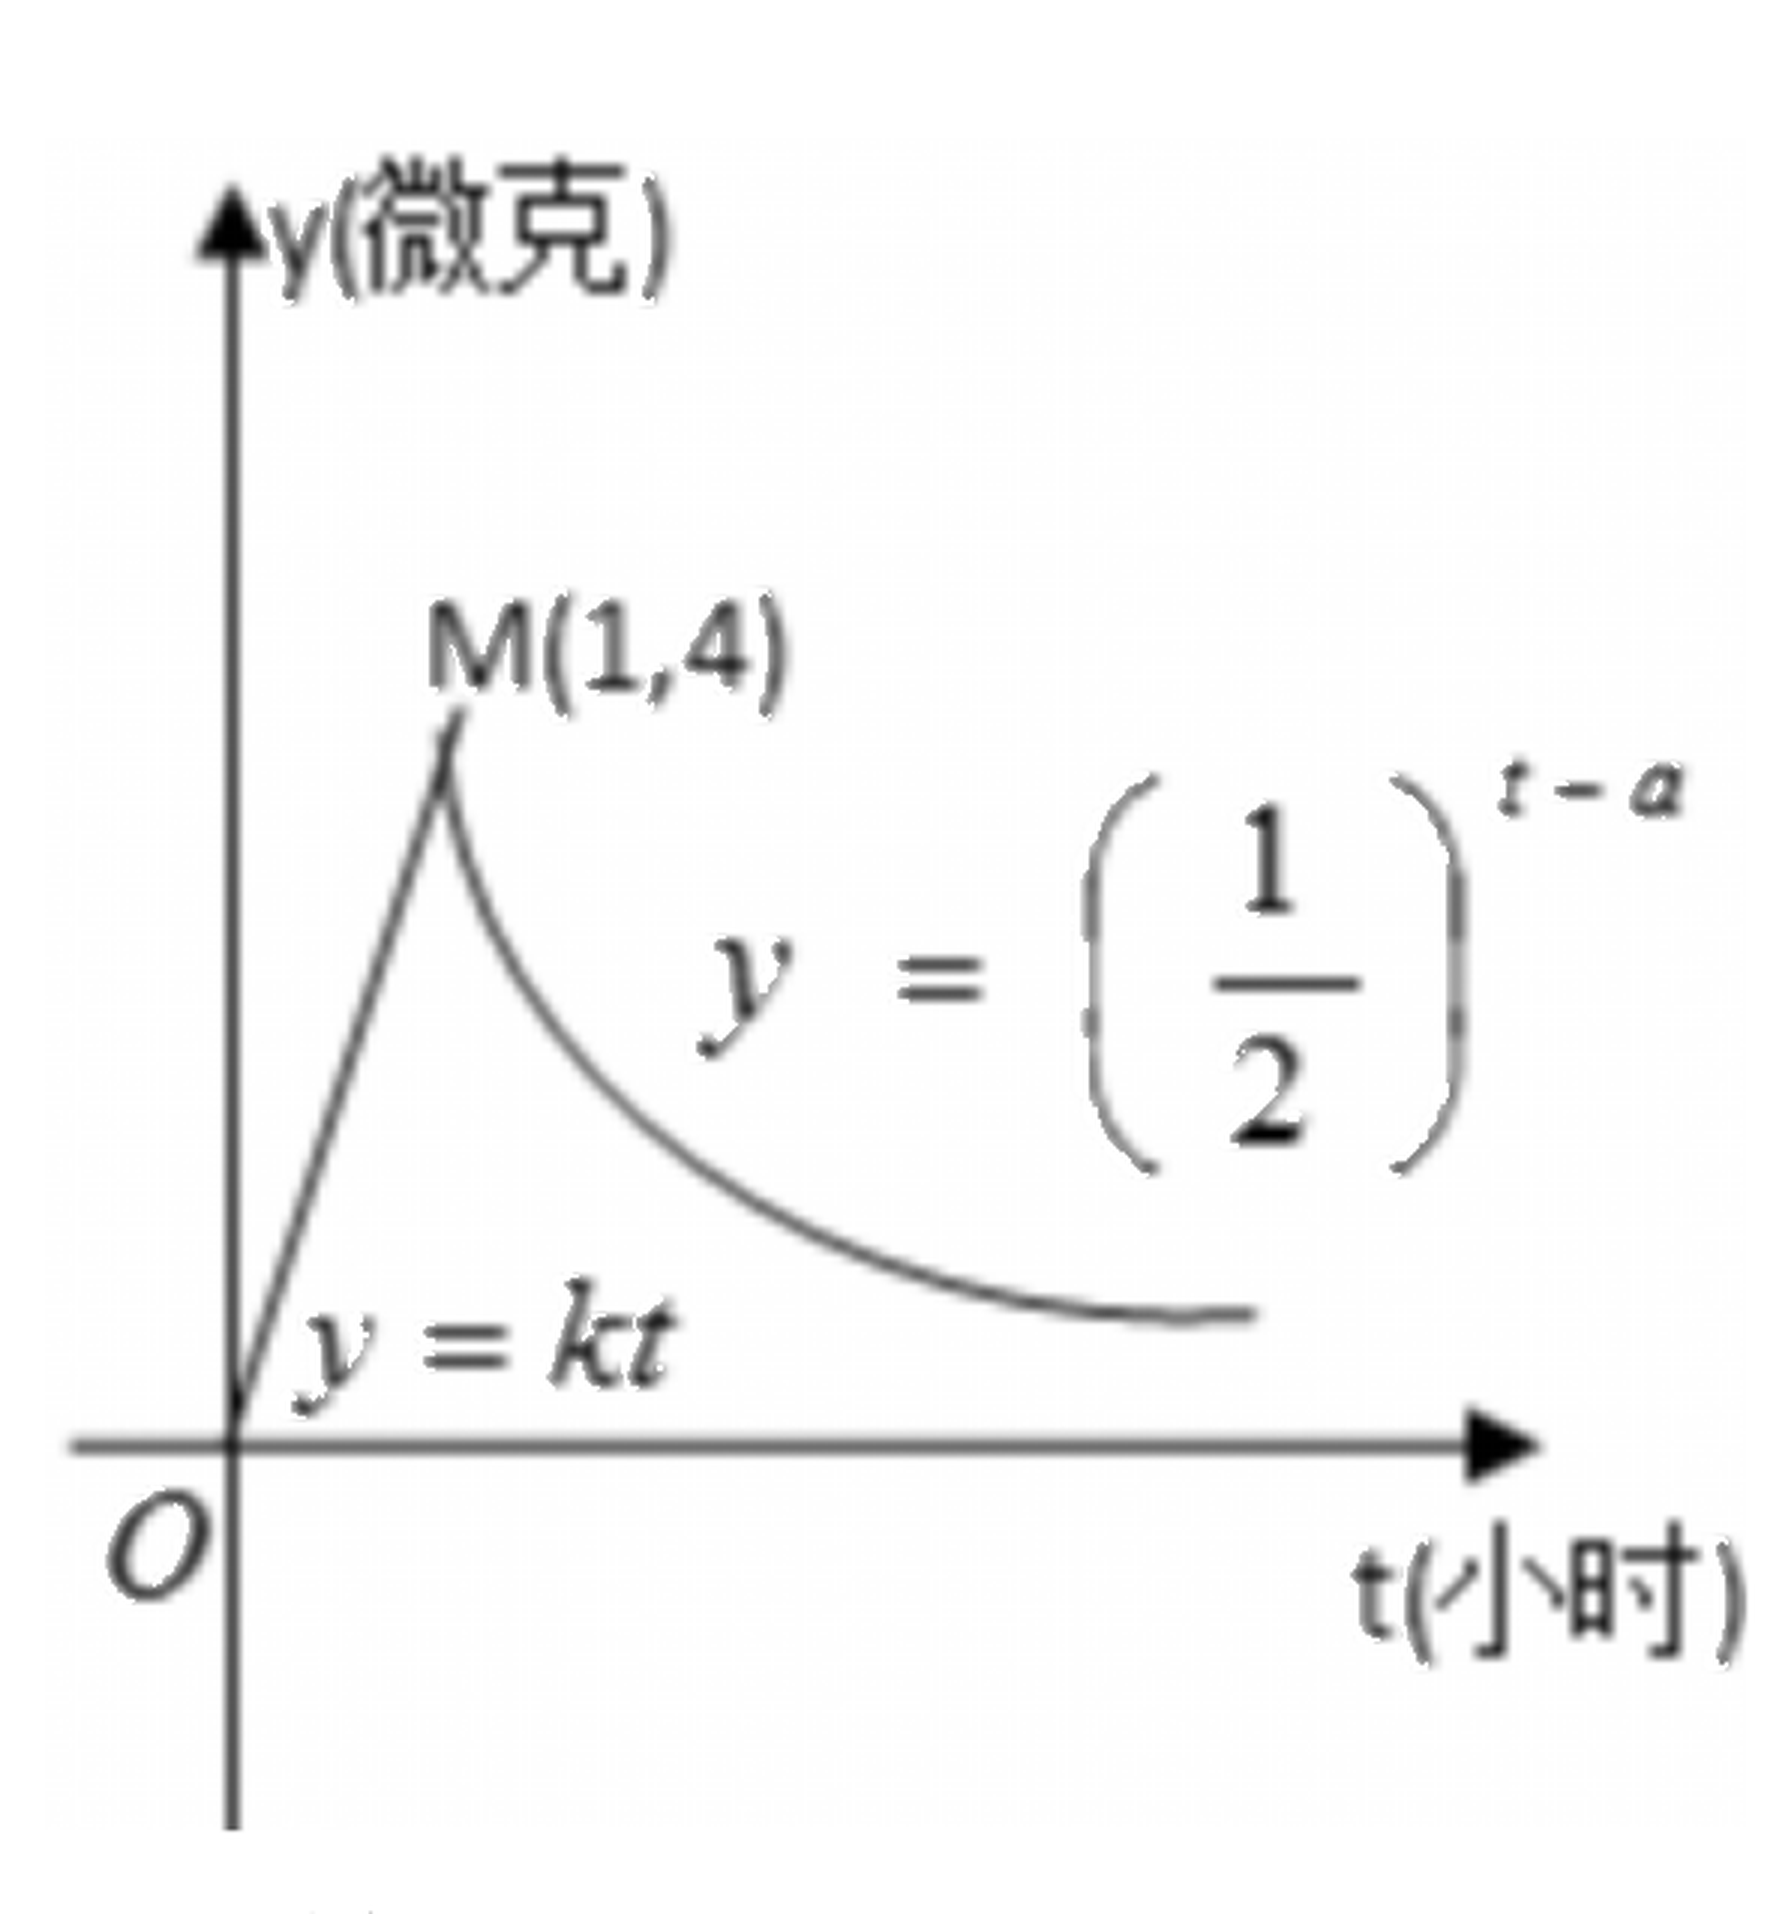
\includegraphics[width=0.42\textwidth]{figures/gao136_q20.png}
\end{center}

\ifanswer
\solbegin
\step{(1) 当 $0\leqslant t\leqslant1$ 时，函数图象是一条线段，由于过原点与点 $(1,4)$，所以 $k=4$，}
\step{其解析式为 $y=4t$，$0\leqslant t\leqslant1$；}
\step{当 $t\geqslant1$ 时，函数的解析式为 $y=\left(\dfrac12\right)^{t-a}$，}
\step{此时 $M(1,4)$ 在曲线上，将此点的坐标代入函数解析式得 $4=\left(\dfrac12\right)^{1-a}$，}
\step{解得 $a=3$；}
\step{(2) 由 (1) 得 $f(t)=\begin{cases}4t,0\leqslant t\leqslant1\\\left(\frac12\right)^{t-3},t>1\end{cases}$；}
\step{(3) 由 (2) 得，令 $f(t)\geqslant0.5$，即 $\begin{cases}4t\geqslant0.5,0\leqslant t\leqslant1\\\left(\frac12\right)^{t-3}\geqslant0.5,t>1\end{cases}$，所以 $\dfrac18\leqslant t\leqslant4$.}
\solend
\fi

\item 已知关于 $x$ 的不等式 $(kx-k^2-4)(x-4)>0$，其中 $k\in\R$.

(1) 当 $k=-1$，求不等式的解集 $A$；

(2) 当 $k$ 变化时，试求不等式的解集 $A$；

(3) 对于不等式解集 $A$，满足 $A\cap\Z=B$. 试探究集合 $B$ 能否为有限集，若能，求出使得集合 $B$ 中元素最少的 $k$ 的所有取值，并用列举法表示此时的集合 $B$，若不能，说明理由；

\ifanswer
\solbegin
\step{(1) 当 $k=-1$ 时，原不等式可化为 $(x+5)(x-4)<0$，}
\step{解得 $-5<x<4$，故不等式的解集为 $\{x\mid -5<x<4\}$；}
\step{(2) 当 $k=0$ 时，解集为 $\{x\mid x<4\}$，}
\step{当 $k>0$ 时，$\dfrac{k^2+4}{k}=k+\dfrac4k\geqslant4$，解集为 $\{x\mid x<4\text{ 或 }x>\dfrac{k^2+4}{k}\}$；}
\step{当 $k<0$ 时，解集为 $\{x\mid \dfrac{k^2+4}{k}<x<4\}$，}
\step{综上，当 $k=0$ 时，$A=\{x\mid x<4\}$，}
\step{当 $k>0$ 时，$A=\{x\mid x<4\text{ 或 }x>\dfrac{k^2+4}{k}\}$；}
\step{当 $k<0$ 时，$A=\{x\mid \dfrac{k^2+4}{k}<x<4\}$，}
\step{(3) 由 (2) 得当 $k\geqslant0$ 时，$B$ 为无限集，当 $k<0$ 时，$B$ 为有限集，}
\step{此时，$\dfrac{k^2+4}{k}=k+\dfrac4k\leqslant-4$，当且仅当 $k=-2$ 时取等号，}
\step{所以 $k=-2$ 时，$B$ 中元素最少，此时 $A=\{x\mid -4<x<4\}$，}
\step{所以 $B=\{-3,-2,-1,0,1,2,3\}$.}
\solend
\fi

\end{enumerate}

% 第 22 题是"四、附加题"首题且带 9cm 图块，守卫须放在 \bigsec 之前连节标题一起量，
% 否则"四、附加题"会孤立在页末（B 类，照 高一26／40／59 成例）
\needvspace{11cm}
\bigsec{四、附加题}

\begin{enumerate}
\setcounter{enumi}{21}

% 第 22 题四幅抛物线/坐标图选项是一整块，守卫放在 \item 之前
\needvspace{9cm}
\item 函数 $f(x)=\left(\dfrac12\right)^{\lvert x+1\rvert}$ 的图象大致为\mbox{（\quad）}

\keepwithprev
\begin{center}
% 四幅抛物线/坐标图选项取原卷 07 页截图去粉色水印，按原卷 2x2 排布合并为一张
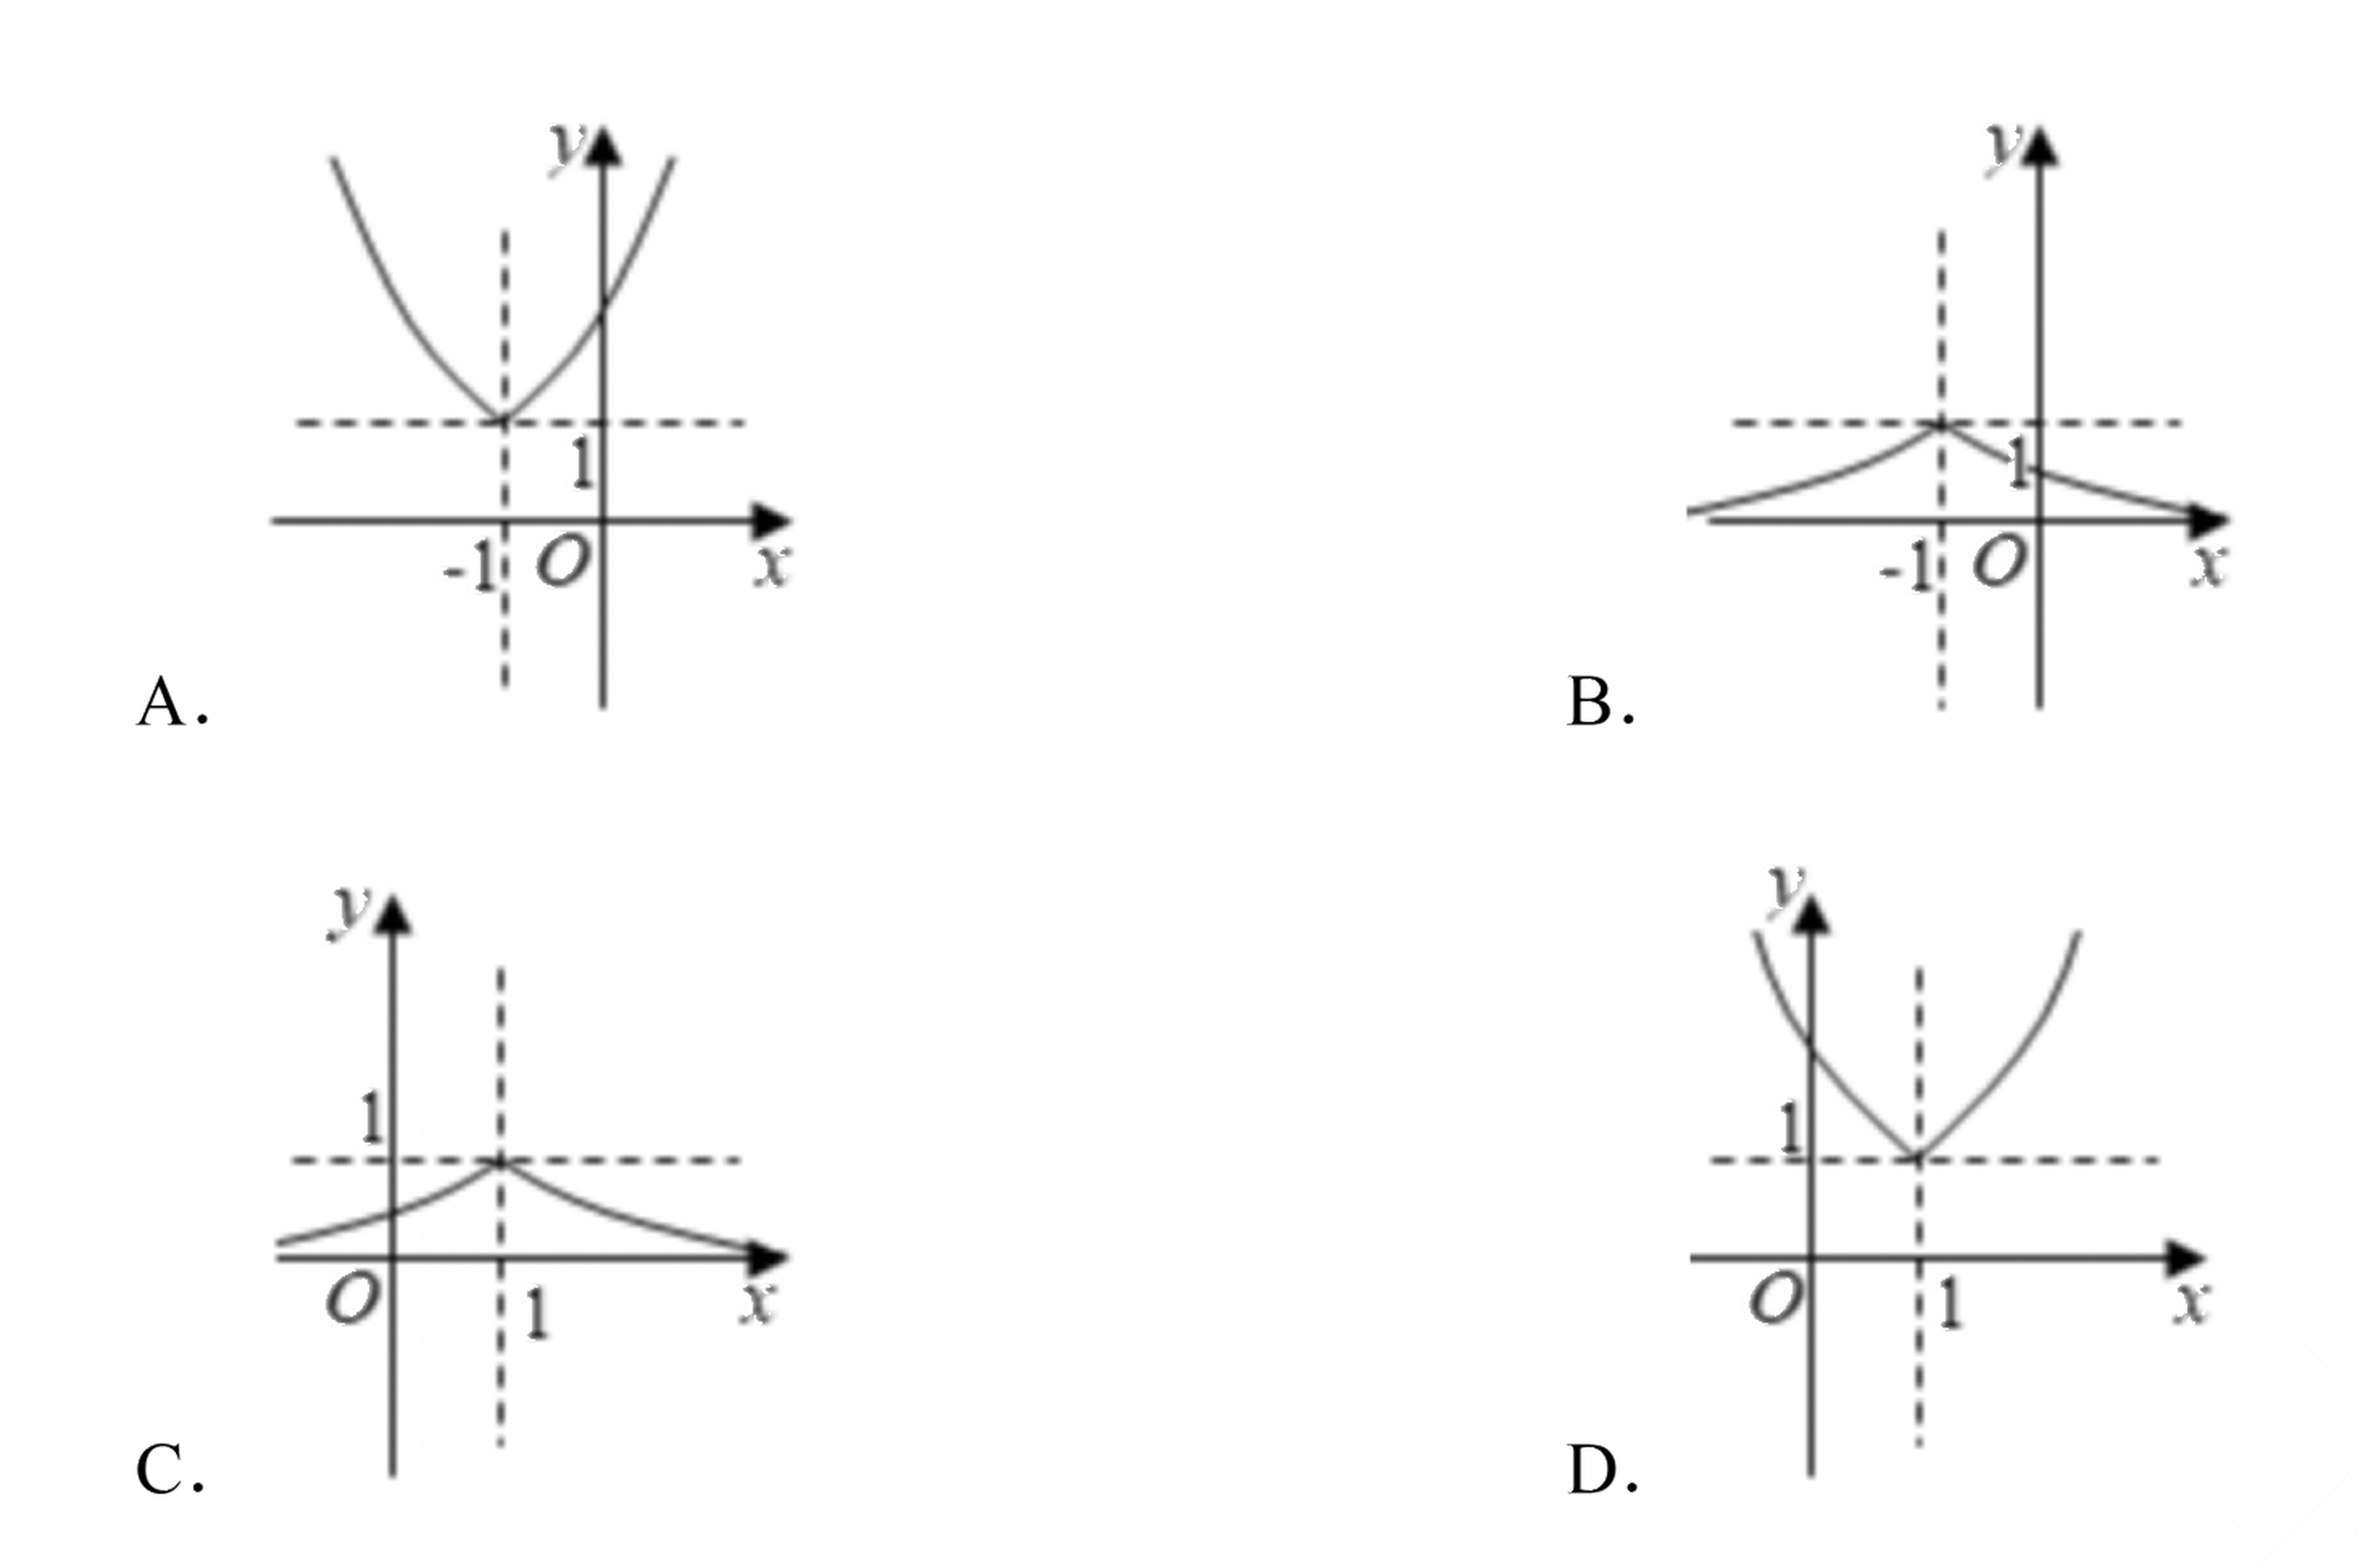
\includegraphics[width=0.80\textwidth]{figures/gao136_q22.png}
\end{center}

\ifanswer
\ans{$B$}
\fi

\end{enumerate}

\end{document}
"
%
% ① 原始材料：微信公众号"魔都数学加油站"文章，作者破晓，2026-11-15 18:04 发布；
% 连载"27学年高一136"，原文标题"27学年高一136——2026-2027年上海市三林中学高一上期中"；
% 原文链接：https://mp.weixin.qq.com/s/jaMzqMm6pDvcT0yM0d7eaQ。
% 正文为 7 张 PNG 页（01、04、06 为 4762x6735；02、03、05、07 为 2560x3620，
% 同一篇各页分辨率不同，逐页按各自分辨率裁图核对），题目下印有【答案】或【解析】，为讲评版。
% 题目、解析均据原图转录；卷面粉红色水印"魔都数学加油站"及公众号页脚未录入。
% 全卷 3 幅插图：第 13 题四幅坐标图选项（03 页）、第 20 题药物浓度折线/曲线图（05 页）、
% 第 22 题四幅抛物线/坐标图选项（07 页），均取原卷截图去粉色水印、去色、LANCZOS 放大，
% 四幅选项按原卷 2x2 排布合并为一张；图前按惯例加 \needvspace 守卫。
%
% 卷首标题：原卷印作"2026-2027 年三林中学高一上期中"（公众号标题中的"上海市"
% 卷面标题行没有，本稿照卷面），年份区间按全稿惯例排 en dash；原卷未印副标题，
% 本卷为期中卷、跨集合与常用逻辑用语／不等式／函数三章，按题目内容标为
% "集合与常用逻辑用语、不等式、函数"（与 125／126／128／129／131／132／133 同期中卷口径相同）：
% 集合与逻辑见 Q3、Q6、Q10、Q12、Q16、Q18、Q21，不等式见 Q5、Q7、Q8、Q9、Q14、Q15，
% 函数（幂函数、指数／对数、基本不等式应用）见 Q4、Q11、Q13、Q17、Q19、Q20、Q22。
%
% 题号体例：本卷共 20 题——一、填空题 3—12（10 题）、二、选择题 13—16（4 题）、
% 三、解答题 17—21（5 题）、四、附加题 22（1 题）。四节分别
% \setcounter{enumi}{2}／{12}／{16}／{21}。
%
% ② 与原卷的排版差异：
%   ① 原文从第 3 题起，本稿保留原题号；末节"四、附加题"另起 \bigsec，题号续到 22；
%   ② 原卷每题下直接印【答案】或【解析】，本稿按全稿惯例置于答案版；第 3、4、6 题只印
%      【答案】、无【解析】，提 \ans{}；第 14 题答案 C 印在题干括号内、无【解析】，按
%      高一53／高一108／高一132／高一133 成例括号留空、另提 \ans{$C$}；第 22 题答案 B
%      印在题干括号内、无【解析】，同例提 \ans{$B$}；第 13、15、16 题答案在解析末句
%      "故选 …"，括号内留空、不另提 \ans{}；其余各题印【解析】、无独立答案段；
%   ③ 原卷未印副标题，本稿按"知识模块"口径补出；
%   ④ 原卷填空横线按全稿惯例排为 \blankline[4.4em]；选择题括号排 \mbox{（\quad）}、
%      每个选项段前按惯例加 \keepwithprev（四幅图选项那一枚放在 \begin{center} 之前）；
%      解答题不留作答区、不加 \anspace（原卷为讲评版，与 129／131／132／133 同）；
%   ⑤ 原卷数集排斜体 $R$／$R^+$／$Z$，按全稿惯例改 \R／\R^+／\Z；空集记号 \varnothing；
%      绝对值排 \lvert…\rvert，集合描述竖线排 \mid；不等号按全稿惯例排 \leqslant／\geqslant；
%   ⑥ 子题标号 (1)(2)(3) 原卷用半角括号，照录；圈数字 ①②③④ 照录；第 12 题甲／乙／丙
%      三行与第 14 题四个编号不等式照录；
%   ⑦ 数学式内半角逗号照录（如 Q4"$a>0,a\neq1$"、Q6"$\{(-2,4),(1,1)\}$"、
%      Q7"$a=2+3=5,b=2\times3=6$"、Q11"$x_1,x_2$"、Q12"$m,n\in R^+$"、
%      Q15"$a>1,b\geq0$"、Q18"$B=(2a,a+1)$"、Q20"$4t,0\leq t\leq1$"、
%      Q21"$\{-3,-2,-1,0,1,2,3\}$"）；原卷行末西文句点照录，行中全角逗号照录；
%   ⑧ 三幅插图：第 13 题四幅坐标图选项合并裁为一张 \includegraphics（题前 \needvspace{9cm}）；
%      第 20 题折线/曲线图取 05 页截图（0.42\textwidth）；第 22 题四幅抛物线/坐标图选项合并
%      裁为一张（题前 \needvspace{9cm}）。第 13、22 题分别是"二、选择题""四、附加题"的首题
%      且带大图块，另在两处 \bigsec 之前各加 \needvspace{11cm} 连节标题一起量，避免节标题
%      孤立在页末（切页审计 B 类；照 高一26／40／59 成例）。第 20 题图不是节首题、三版试排
%      图均与题干同页，加 7cm 守卫反会多出一张只有两行正文的稀疏页，故不另加守卫；
%      三版切页审计均"合计异常：无"（试卷 4 页／紧凑 4 页／答案 6 页）；
%   ⑨ 跨页续印按题合并：Q16 题干在 03 页、括号与选项及【解析】在 04 页；Q19 题干在 04 页、
%      (2) 与【解析】在 05 页；Q20 (3)【解析】在 06 页；Q22 四幅图在 07 页；本稿按题连排；
%   ⑩ 题干中的中文弯引号按原卷照录，注释内一律 ASCII 引号；原卷"图像／图象"两种写法混用，
%      逐处照录（Q4、Q19 作"图像"，Q13、Q15、Q20、Q22 作"图象"）；
%   ⑪ 附加题节：原卷印"四、附加题"，本稿用 \bigsec{四、附加题} 另起一节、
%      \setcounter{enumi}{21}，顶层 1 个 \item（与 高一09／15／16／22／35／39／47／61 同口径）；
%      Q22 只印括号内答案、提 \ans{}，不计入 \step 账。
%
% 判别式字形：全卷仅第 9 题【解析】cases 块出现判别式"$\Delta=a^2-8a<0$"，原卷印
%   等腰、偏高的三角 $\Delta$，逐处放大核对并照录 \Delta；全卷未出现扁等边三角 \triangle。
%
% 子集符号：第 18 题 (2) 题干"$B\subseteq A$"与【解析】"$B\subseteq A$"两处原卷均印
%   带下划线 $\subseteq$，逐处放大核对、照录 \subseteq；全卷未出现单线 \subset。
%
% 原卷存疑照录（均照录未改，正文对应处另有 % 注）：
%   第 12 题乙行"$\dfrac{m+n}{mm}=\dfrac1{mn}$"前一分母印作 $mm$（后一处作 $mn$），照录；
%   第 12 题【解析】"$\geqslant\dfrac1{100}\left[a^2+1+2\sqrt{a^2}\right]$"保留 $\sqrt{a^2}$
%      未化简为 $a$，照录；
%   第 13 题【解析】"排除 BC"与"排除 D"连写选项字母，照录；
%   第 18 题 (2)【解析】末行"所以实数 $a$ 的取值范围 $(-\infty,-2]\cup[\frac12,1)$"
%      "取值范围"后脱"是／为"字，照录；
%   第 21 题 (3) 题干"求出使得集合 $B$ 中元素最少的 $k$ 的所有取值"而【解析】只给出
%      $k=-2$ 一处，措辞照录。
%
% 行数复核：逐题数 \step 条数，合计 51 条（Q3：0；Q4：0；Q5：2；Q6：0；Q7：2；Q8：1；
% Q9：1；Q10：4；Q11：1；Q12：4；Q13：2；Q14：0；Q15：2；Q16：3；Q17：1；Q18：5；
% Q19：4；Q20：7；Q21：12；Q22：0），与原卷印刷行逐题相等（cases 块作一个印刷行计）。
% 第 3、4、6、14、22 题只印【答案】、提 \ans{}，不计入 \step 账；第 13、15、16 题答案在
% 解析末句，括号内留空、不另提 \ans{}。
%
\documentclass[a4paper,11pt]{article}
\usepackage{common}

\begin{document}

\examtitlest[3]{2026--2027 年三林中学高一上期中}{集合与常用逻辑用语、不等式、函数}

\bigsec{一、填空题}

\begin{enumerate}
\setcounter{enumi}{2}

\item 用反证法证明命题“若 $x+y\neq5$，则 $x\neq2$ 或 $y\neq3$”为真命题时，第一个步骤是\blankline[4.4em].

\ifanswer
\ans{假设 $x=2$ 且 $y=3$}
\fi

\item 函数 $y=a^{x-1}+1(a>0,a\neq1)$ 的图像恒过定点 $A$，则点的坐标是\blankline[4.4em].

\ifanswer
\ans{$(1,2)$}
\fi

\item 已知 $x>1$，则 $x+\dfrac4{x-1}$ 的最小值是\blankline[4.4em].

\ifanswer
\solbegin
\step{由 $x>1$，得 $x-1>0$，则 $x+\dfrac4{x-1}=x-1+\dfrac4{x-1}+1\geqslant2\sqrt{(x-1)\cdot\dfrac4{x-1}}+1=5$，}
\step{当且仅当 $x-1=\dfrac4{x-1}$ 即 $x=3$ 时取等号，取得最小值 $5$.}
\solend
\fi

\item 已知集合 $A=\{(x,y)\mid y=x^2\}$，集合 $B=\{(x,y)\mid y=2-x\}$，求 $A\cap B=$\blankline[4.4em].

\ifanswer
\ans{$\{(-2,4),(1,1)\}$}
\fi

\item 已知一元二次不等式 $x^2-ax+b<0$ 的解集为 $(2,3)$，则不等式 $bx^2-ax+1>0$ 的解集是\blankline[4.4em].

\ifanswer
\solbegin
\step{$a=2+3=5,b=2\times3=6$，则 $bx^2-ax+1>0$ 即 $6x^2-5x+1>0$，}
\step{即 $(3x-1)(2x-1)>0$，解集为 $\left(-\infty,\dfrac13\right)\cup\left(\dfrac12,+\infty\right)$.}
\solend
\fi

\item 不等式 $(x+2)^3<(5-2x)^3$ 的解集为\blankline[4.4em].

\ifanswer
\solbegin
\step{由 $(x+2)^3<(5-2x)^3$ 得 $x+2<5-2x$，故解集为 $(-\infty,1)$.}
\solend
\fi

\item 若关于 $x$ 的不等式 $ax^2-ax+2>0$ 的解集为 $\R$，则实数 $a$ 的取值范围是\blankline[4.4em].

\ifanswer
\solbegin
\step{由题意得 $a=0$ 或 $\begin{cases}a>0\\\Delta=a^2-8a<0\end{cases}$，所以 $0\leqslant a<8$.}% 判别式原卷印高三角 $\Delta$，照录
\solend
\fi

\item 已知关于 $x$ 的不等式 $\lvert x+3\rvert+\lvert x-a\rvert\geqslant5$ 恒成立，则实数 $a$ 的取值范围为\blankline[4.4em].

\ifanswer
\solbegin
\step{因为 $\lvert x+3\rvert+\lvert x-a\rvert\geqslant\lvert x-a-x-3\rvert=\lvert 3+a\rvert$，}
\step{要使 $\lvert x+3\rvert+\lvert x-a\rvert\geqslant5$ 恒成立，则 $\lvert a+3\rvert\geqslant5$ 即可，}
\step{所以 $a+3\geqslant5$ 或 $a+3\leqslant-5$，解得 $a\geqslant2$ 或 $a\leqslant-8$，}
\step{即实数 $a$ 的取值范围是 $(-\infty,-8]\cup[2,+\infty)$.}
\solend
\fi

\item 若方程 $\lg^2 x-2\lg x-2=0$ 的两个解为 $x_1,x_2$，求 $\log_{x_1}x_2+\log_{x_2}x_1$ 的值为\blankline[4.4em].

\ifanswer
\solbegin
\step{$\log_{x_1}x_2+\log_{x_2}x_1=\dfrac{\lg x_2}{\lg x_1}+\dfrac{\lg x_1}{\lg x_2}=\dfrac{(\lg x_1+\lg x_2)^2-2\lg x_1\lg x_2}{\lg x_1\lg x_2}=-4$.}
\solend
\fi

\item 三个同学对问题“已知 $m,n\in \R^+$，且 $m+n=1$，求 $\dfrac1m+\dfrac1n$ 的最小值”提出各自的解题思路：

思路：

甲：$\dfrac1m+\dfrac1n=\dfrac{m+n}{m}+\dfrac{m+n}{n}=2+\dfrac nm+\dfrac mn$，可用基本不等式求解；

乙：$\dfrac1m+\dfrac1n=\dfrac{m+n}{mm}=\dfrac1{mn}=\dfrac1{m(1-m)}$，可用二次函数配方法求解；% 原卷前一分母印作 $mm$，照录

丙：$\dfrac1m+\dfrac1n=\left(\dfrac1m+\dfrac1n\right)(m+n)=2+\dfrac nm+\dfrac mn$，可用基本不等式求解；参考上述解题思路，

可求得当 $x=$\blankline[4.4em]时，$y=\dfrac{a^2}{x^2}+\dfrac1{100-x^2}$（$0<x<10$，$a>0$）有最小值.

\ifanswer
\solbegin
\step{$y=\dfrac{a^2}{x^2}+\dfrac1{100-x^2}=\left(\dfrac{a^2}{x^2}+\dfrac1{100-x^2}\right)[x^2+(100-x^2)]\times\dfrac1{100}$}
\step{$=\dfrac1{100}\left[a^2+1+\dfrac{x^2}{100-x^2}+\dfrac{a^2(100-x^2)}{x^2}\right]\geqslant\dfrac1{100}\left[a^2+1+2\sqrt{a^2}\right]$}% 原卷保留 $\sqrt{a^2}$ 未化简，照录
\step{当且仅当 $\dfrac{x^2}{100-x^2}=\dfrac{a^2(100-x^2)}{x^2}$，即 $x=\sqrt{\dfrac{100a}{a+1}}$ 时，}
\step{$y=\dfrac{a^2}{x^2}+\dfrac1{100-x^2}(0<x<10,a>0)$ 有最小值.}
\solend
\fi

\end{enumerate}

% 第 13 题是"二、选择题"首题且带 9cm 图块，守卫须放在 \bigsec 之前连节标题一起量，
% 否则"二、选择题"会孤立在页末（B 类，照 高一26／40／59 成例）
\needvspace{11cm}
\bigsec{二、选择题}

\begin{enumerate}
\setcounter{enumi}{12}

% 第 13 题四幅坐标图选项是一整块，守卫放在 \item 之前
\needvspace{9cm}
\item 下列图象中，最符合函数 $y=x^{\frac54}$ 的图象的是\mbox{（\quad）}

\keepwithprev
\begin{center}
% 四幅坐标图选项取原卷 03 页截图去粉色水印，按原卷 2x2 排布合并为一张
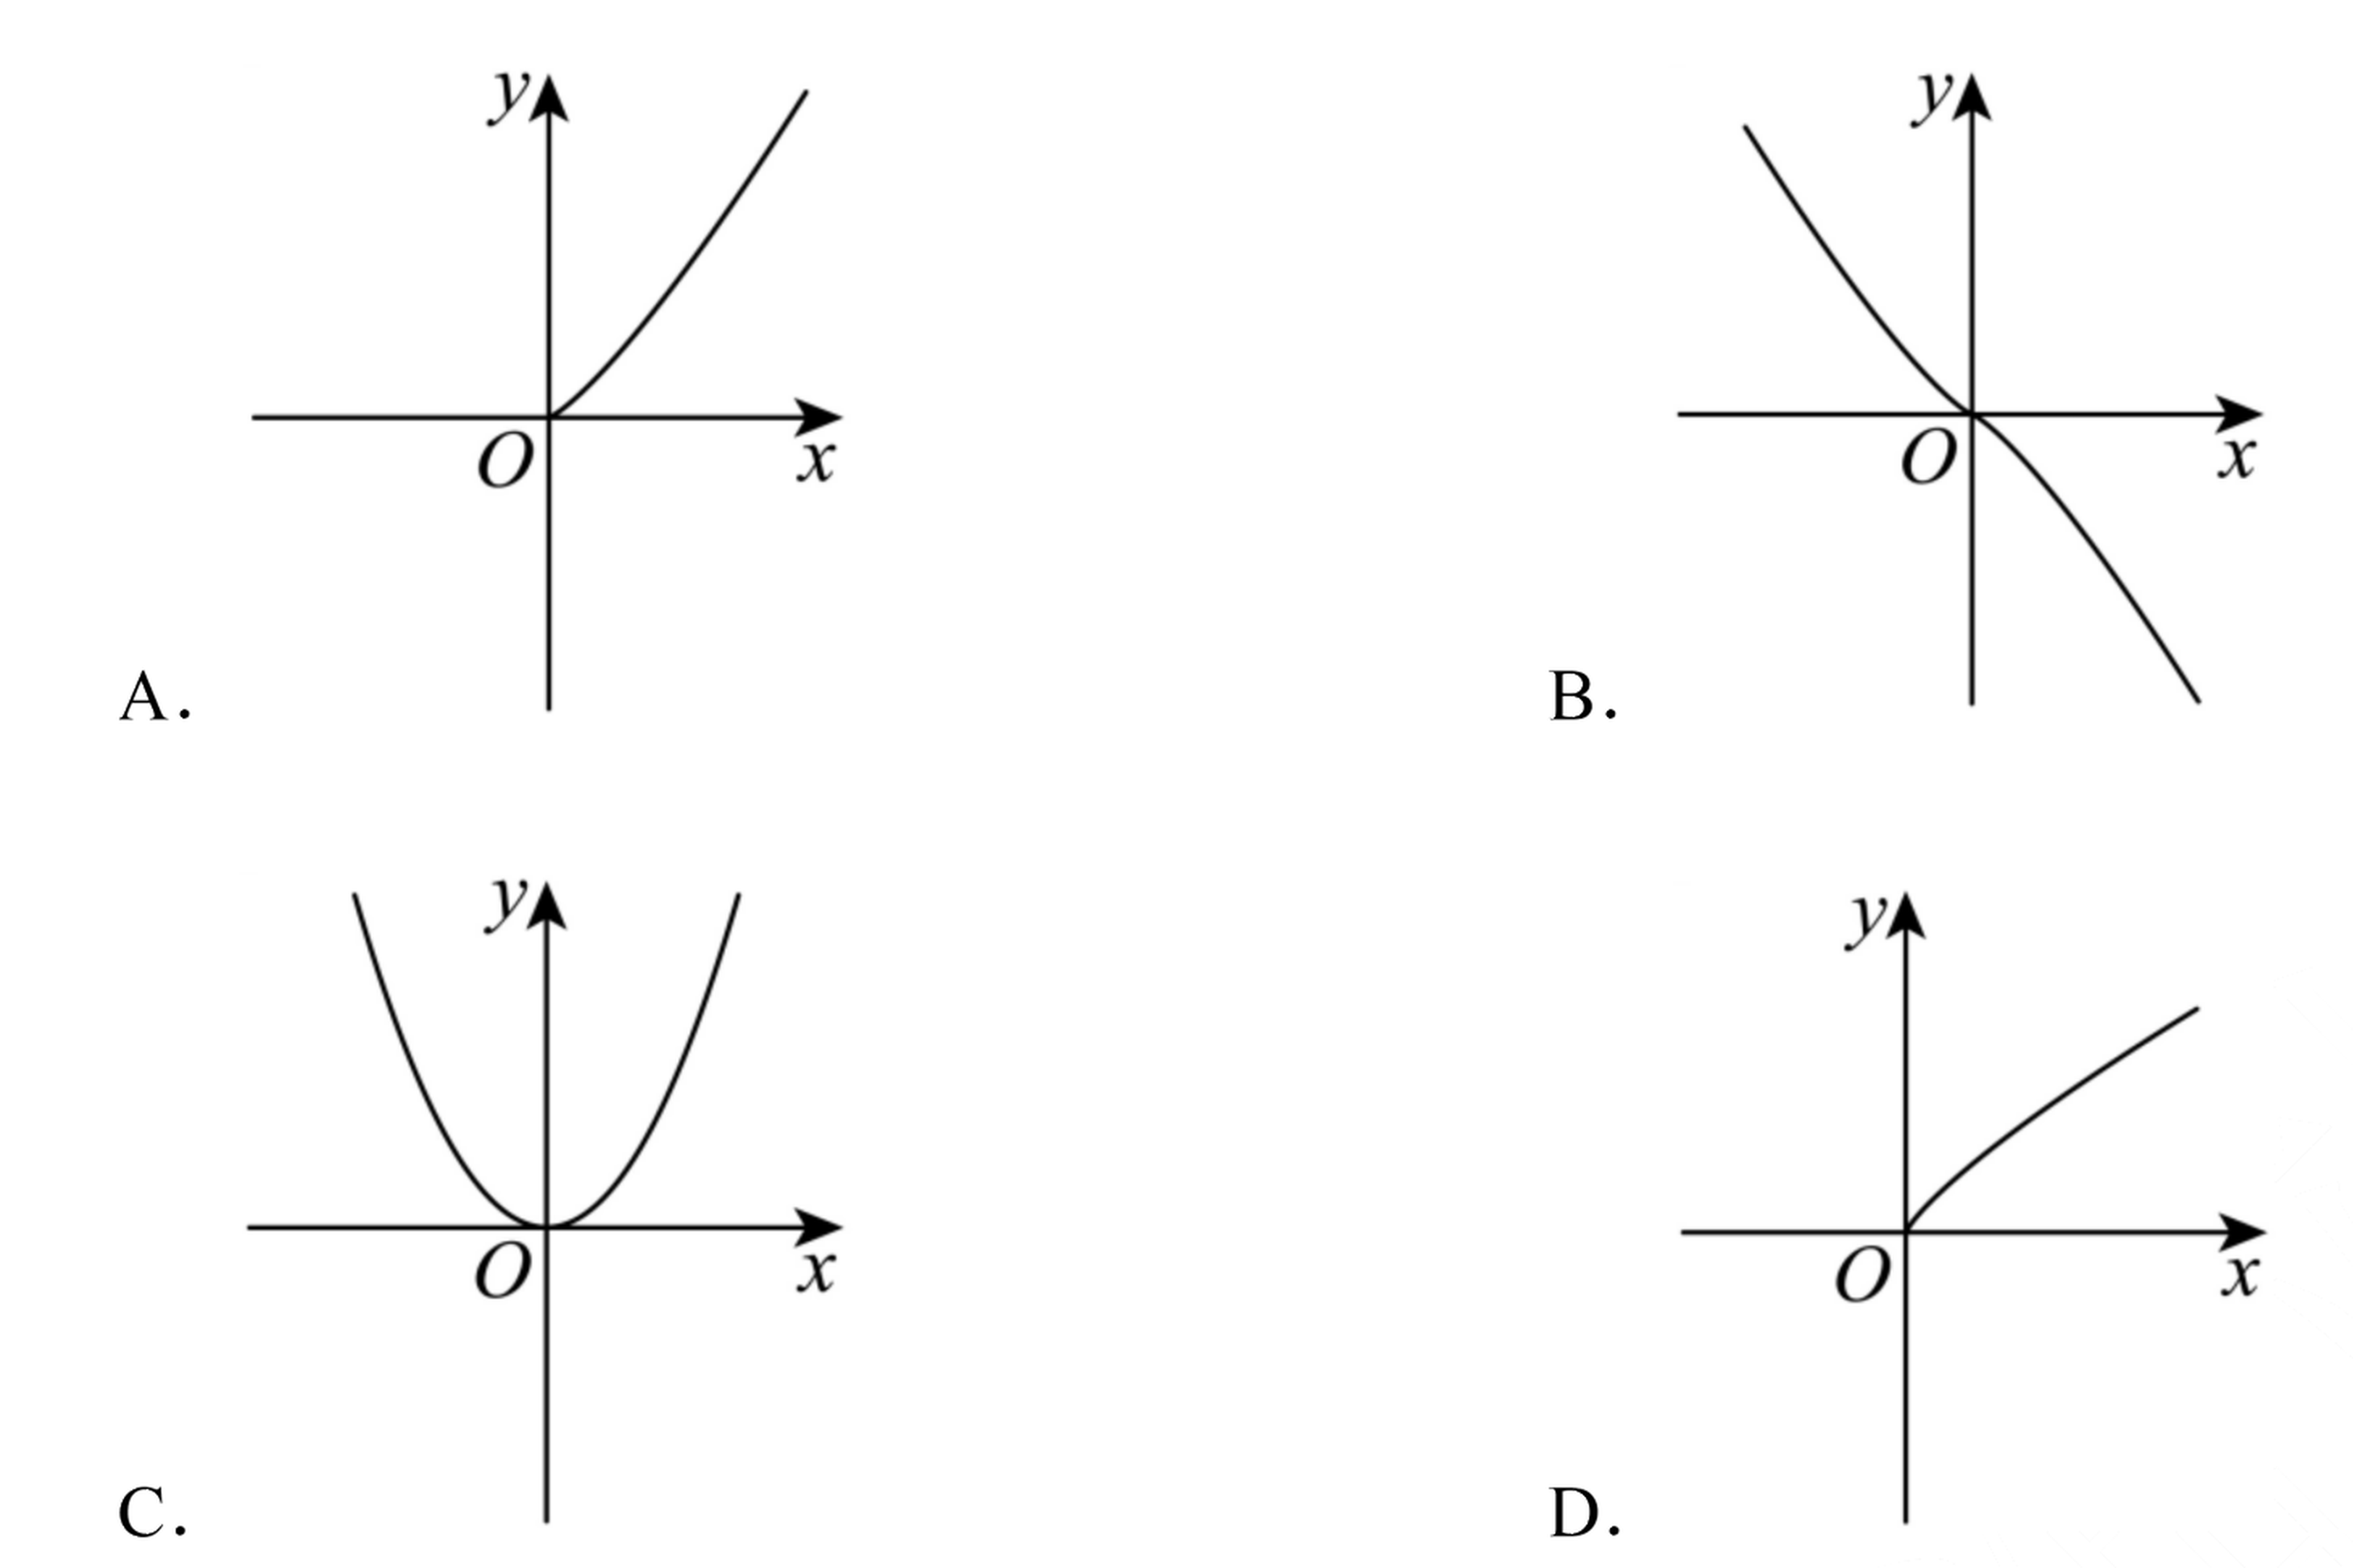
\includegraphics[width=0.80\textwidth]{figures/gao136_q13.png}
\end{center}

\ifanswer
\solbegin
\step{由 $y=x^{\frac54}=\sqrt[4]{x^5}$，函数的定义域为 $[0,+\infty)$，排除 BC，}% 原卷"排除 BC"连写，照录
\step{因为 $\dfrac54>1$，所以函数 $y=x^{\frac54}$ 的图象呈现下凸的趋势，排除 D. 故选 $A$.}
\solend
\fi

\item 下列不等式① $a+\dfrac1a\geqslant2$；② $a^2+4\geqslant4a$；③ $\left\lvert\dfrac ba+\dfrac ab\right\rvert\geqslant2$；④ $\dfrac{2a^2b^2}{a^2+b^2}\leqslant ab$；其中恒成立的是\mbox{（\quad）}

\keepwithprev
A. ①④\qquad B. ③④\qquad C. ②③\qquad D. ①②

\ifanswer
\ans{$C$}
\fi

\item 函数 $y=a^x+b-1(a>0,a\neq1)$ 单调递增且图象不经过第四象限，则 $a,b$ 满足的条件为\mbox{（\quad）}

\keepwithprev
A. $a>1,b\leqslant1$\qquad B. $a>1,b\geqslant0$\qquad C. $0<a<1,b\leqslant1$\qquad D. $0<a<1,b\geqslant1$

\ifanswer
\solbegin
\step{因为函数 $y=a^x+b-1$ 单调递增，所以 $a>1$，}
\step{图象不经过第四象限，则 $x=0$ 时，$y=b\geqslant0$，所以 $a>1,b\geqslant0$，故选 $B$.}
\solend
\fi

\item 设关于 $x$ 的不等式 $\dfrac{ax-1}{x^2-a}<0$ 的解集为 $S$，且 $3\in S$，$4\notin S$，则实数 $a$ 的取值范围为\mbox{（\quad）}

\keepwithprev
A. $(-\infty,-\sqrt3)\cup\left(\dfrac13,\sqrt3\right)$\qquad B. $\left(-\infty,\dfrac14\right)\cup(16,+\infty)$

C. $\left[\dfrac14,\dfrac13\right)\cup(9,16]$\qquad D. 不能确定

\ifanswer
\solbegin
\step{若 $3\in S$，则 $\dfrac{3a-1}{9-a}<0$，解得 $a\in\left(-\infty,\dfrac13\right)\cup(9,+\infty)$，}
\step{若 $4\notin S$，则 $16-a=0$ 或 $\dfrac{4a-1}{16-a}\geqslant0$，解得 $a\in\left[\dfrac14,16\right]$，}
\step{故实数 $a$ 的取值范围为 $\left[\dfrac14,\dfrac13\right)\cup(9,16]$，故选 $C$.}
\solend
\fi

\end{enumerate}

\bigsec{三、解答题}

\begin{enumerate}
\setcounter{enumi}{16}

\item 计算：(1) 计算 $\dfrac{\lg8+\lg125-\lg2-\lg5}{\lg\sqrt{10}\cdot\lg0.1}$；(2) 若 $a^{2x}=2(a>0)$，求 $\dfrac{a^{3x}+a^{-3x}}{a^x+a^{-x}}$.

\ifanswer
\solbegin
\step{(1) 原式 $=\dfrac{2-1}{\frac12\cdot(-1)}=-2$；(2) 原式 $=a^{2x}-1+a^{-2x}=2-1+\dfrac12=\dfrac32$.}
\solend
\fi

\item 不等式 $\dfrac{x-1}{x+1}\geqslant0$ 的解集为 $A$，不等式 $(x-a-1)(2a-x)>0(a<1)$ 的解集为 $B$.

(1) 求集合 $A$；

(2) 若 $B\subseteq A$，求实数 $a$ 的取值范围.

\ifanswer
\solbegin
\step{(1) $A=(-\infty,-1)\cup[1,+\infty)$.}
\step{(2) 由 $(x-a-1)(2a-x)>0(a<1)$，得 $(x-a-1)(x-2a)<0(a<1)$，}
\step{因为 $a<1$，所以 $a+1>2a$，所以 $B=(2a,a+1)$，}
\step{因为 $B\subseteq A$，所以 $2a\geqslant1$ 或 $a+1\leqslant-1$，即 $a\geqslant\dfrac12$ 或 $a\leqslant-2$，}
\step{而 $a<1$，所以实数 $a$ 的取值范围 $(-\infty,-2]\cup\left[\dfrac12,1\right)$.}% 原卷"取值范围"后脱"是／为"，照录
\solend
\fi

\item 已知幂函数 $y=x^m(m\in\R)$ 经过点 $\left(4,\dfrac12\right)$.

(1) 求此幂函数的表达式和定义域；

(2) 已知点 $A(a+2,y_1)$，点 $B(3-2a,y_2)(a\in\R)$ 在此幂函数的图像上，且满足 $y_1<y_2$，求实数 $a$ 的取值范围.

\ifanswer
\solbegin
\step{(1) 幂函数 $y=x^m(m\in\R)$ 经过点 $\left(4,\dfrac12\right)$，所以 $4^m=\dfrac12\Rightarrow m=-\dfrac12$，}
\step{所以 $f(x)=x^{-\frac12}$，定义域为 $(0,+\infty)$.}
\step{(2) 由于函数 $f(x)$ 在其定义域 $(0,+\infty)$ 上严格减，}
\step{由 $y_1<y_2$，得 $a+2>3-2a\geqslant0\Rightarrow a\in\left(\dfrac13,\dfrac32\right]$.}
\solend
\fi

% 第 20 题图取 05 页截图（0.42\textwidth、高约 6cm）。试排 \item 前加 7cm 守卫会多出
% 一张只有两行正文的稀疏页，且三版不加守卫时图均与题干、【解析】同页，故不另加守卫
\item 某医药研究所开发一种抗甲流新药，如果成年人按规定的剂量服用，据监测：服药后每毫升血液中的含药量 $y$（微克）与时间 $t$（小时）之间近似满足如图所示的曲线.

(1) 结合图，求 $k$ 与 $a$ 的值；

(2) 写出服药后 $y$ 与 $t$ 之间的函数关系式 $y=f(t)$；

(3) 据进一步测定：每毫升血液中含药量不少于 $0.5$ 微克时治疗疾病有效，求服药一次治疗有效的时间范围？

\begin{center}
% 图取原卷 05 页截图去粉色水印、去色，3x LANCZOS 放大
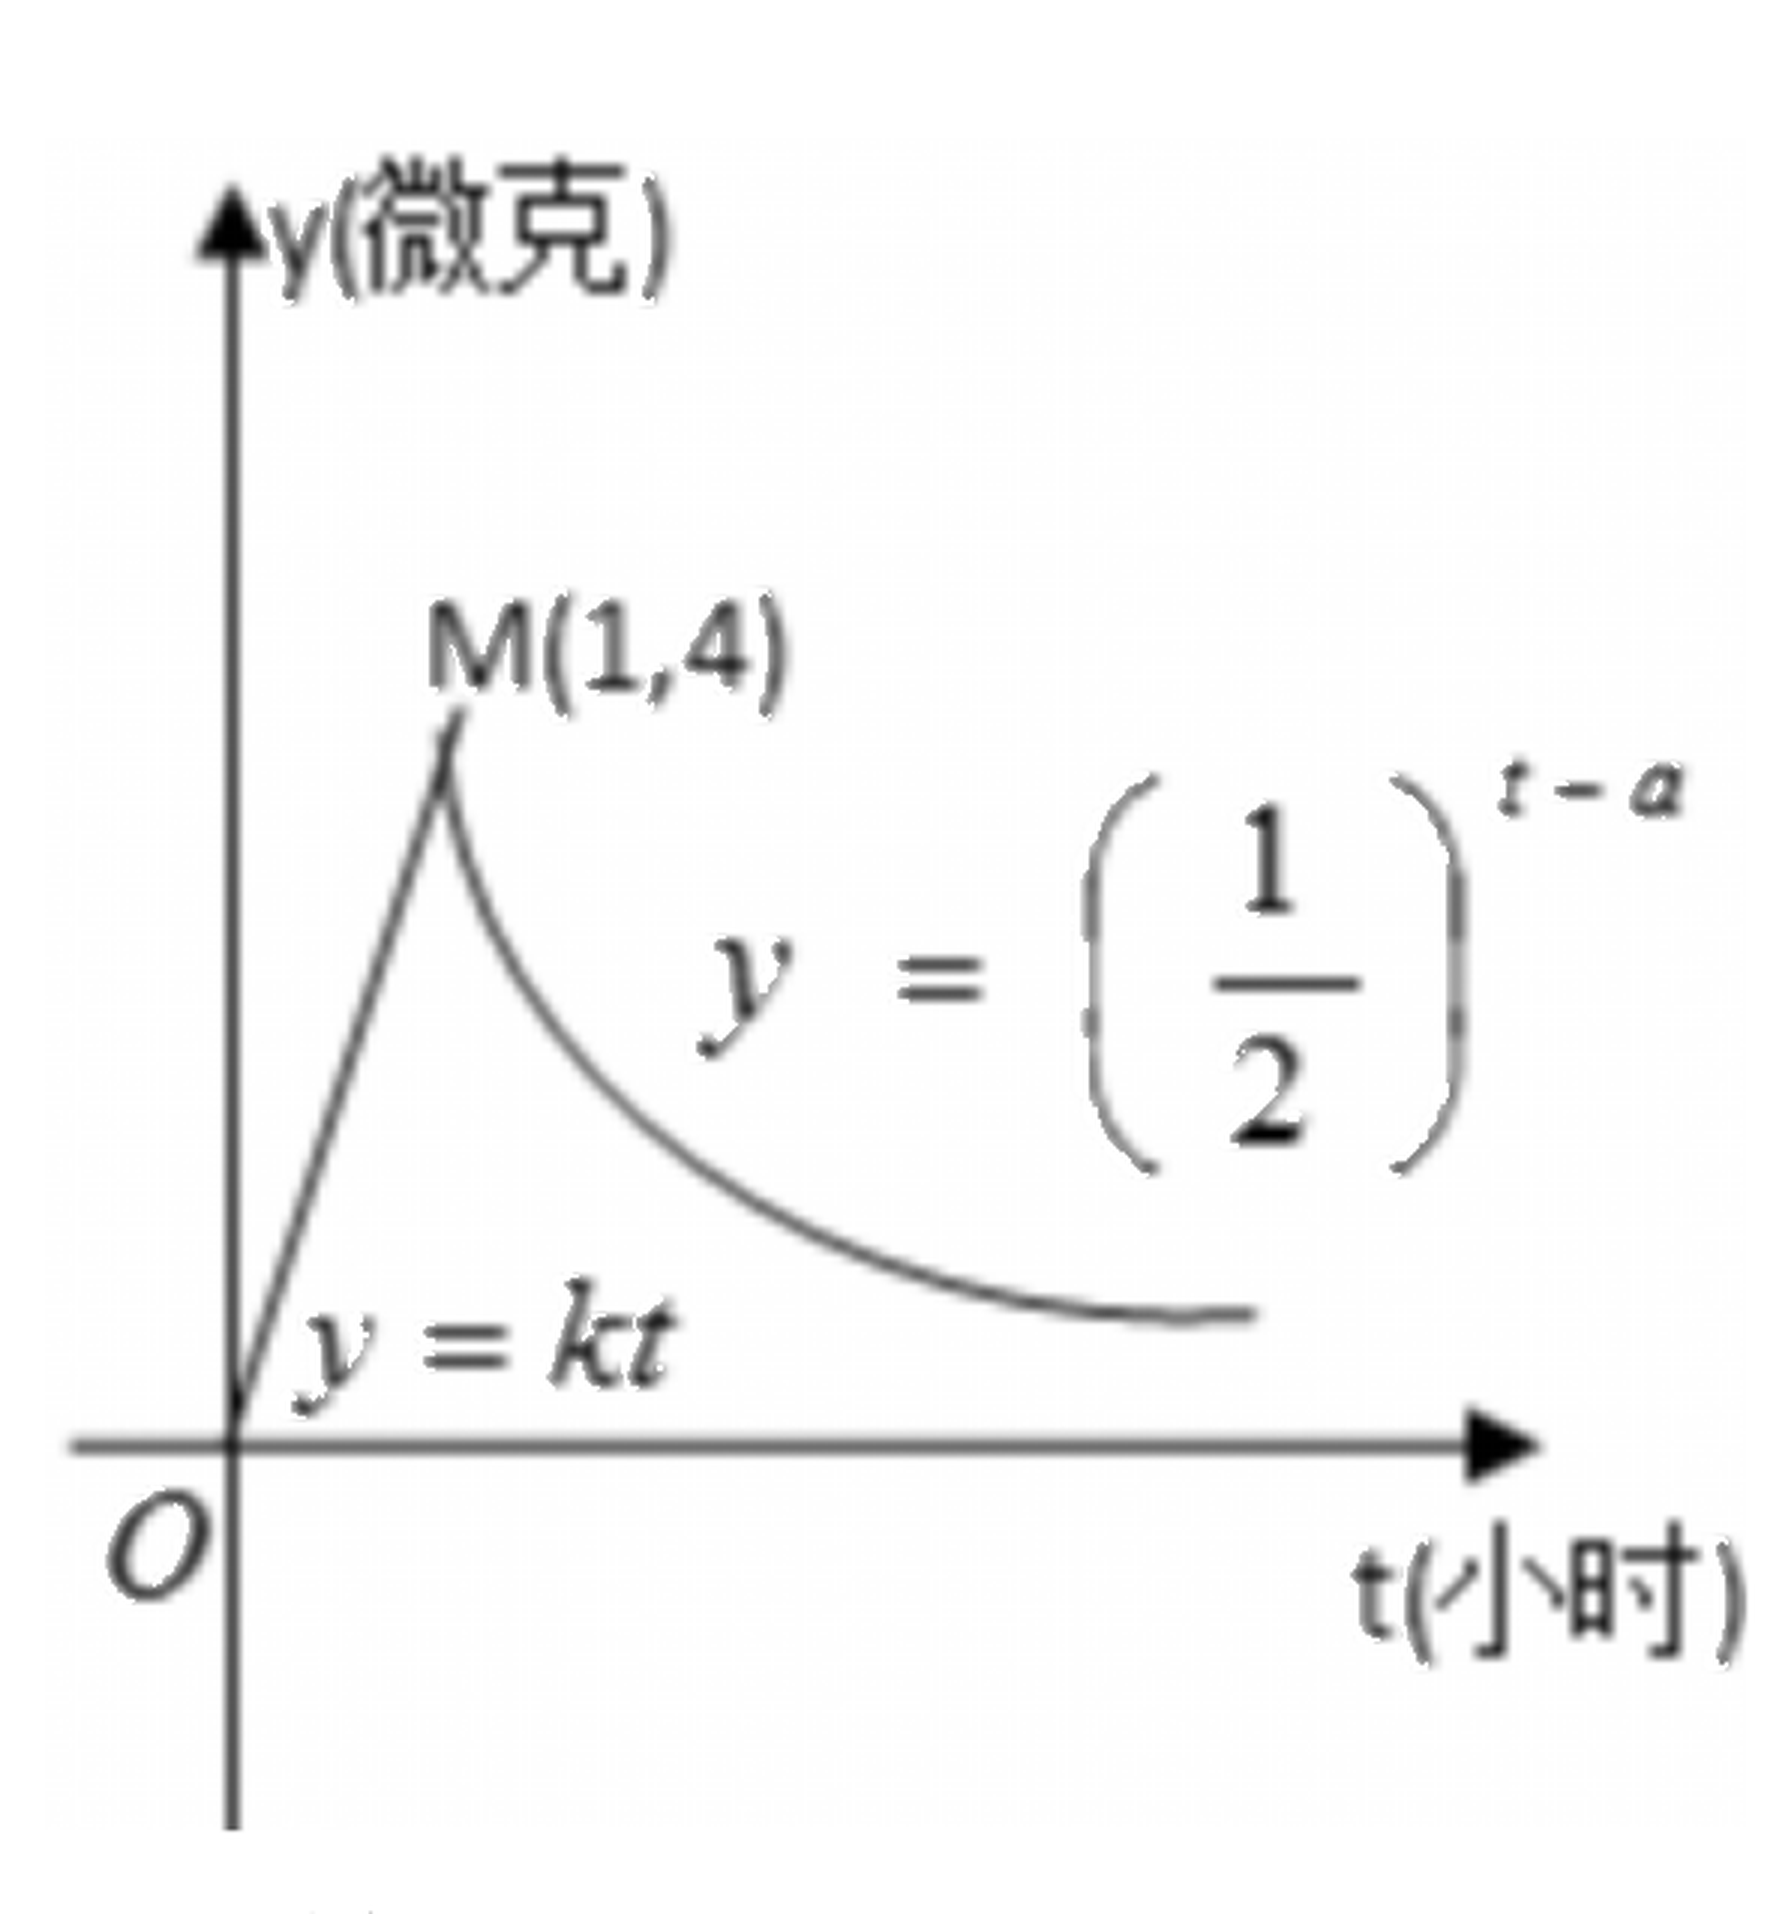
\includegraphics[width=0.42\textwidth]{figures/gao136_q20.png}
\end{center}

\ifanswer
\solbegin
\step{(1) 当 $0\leqslant t\leqslant1$ 时，函数图象是一条线段，由于过原点与点 $(1,4)$，所以 $k=4$，}
\step{其解析式为 $y=4t$，$0\leqslant t\leqslant1$；}
\step{当 $t\geqslant1$ 时，函数的解析式为 $y=\left(\dfrac12\right)^{t-a}$，}
\step{此时 $M(1,4)$ 在曲线上，将此点的坐标代入函数解析式得 $4=\left(\dfrac12\right)^{1-a}$，}
\step{解得 $a=3$；}
\step{(2) 由 (1) 得 $f(t)=\begin{cases}4t,0\leqslant t\leqslant1\\\left(\frac12\right)^{t-3},t>1\end{cases}$；}
\step{(3) 由 (2) 得，令 $f(t)\geqslant0.5$，即 $\begin{cases}4t\geqslant0.5,0\leqslant t\leqslant1\\\left(\frac12\right)^{t-3}\geqslant0.5,t>1\end{cases}$，所以 $\dfrac18\leqslant t\leqslant4$.}
\solend
\fi

\item 已知关于 $x$ 的不等式 $(kx-k^2-4)(x-4)>0$，其中 $k\in\R$.

(1) 当 $k=-1$，求不等式的解集 $A$；

(2) 当 $k$ 变化时，试求不等式的解集 $A$；

(3) 对于不等式解集 $A$，满足 $A\cap\Z=B$. 试探究集合 $B$ 能否为有限集，若能，求出使得集合 $B$ 中元素最少的 $k$ 的所有取值，并用列举法表示此时的集合 $B$，若不能，说明理由；

\ifanswer
\solbegin
\step{(1) 当 $k=-1$ 时，原不等式可化为 $(x+5)(x-4)<0$，}
\step{解得 $-5<x<4$，故不等式的解集为 $\{x\mid -5<x<4\}$；}
\step{(2) 当 $k=0$ 时，解集为 $\{x\mid x<4\}$，}
\step{当 $k>0$ 时，$\dfrac{k^2+4}{k}=k+\dfrac4k\geqslant4$，解集为 $\{x\mid x<4\text{ 或 }x>\dfrac{k^2+4}{k}\}$；}
\step{当 $k<0$ 时，解集为 $\{x\mid \dfrac{k^2+4}{k}<x<4\}$，}
\step{综上，当 $k=0$ 时，$A=\{x\mid x<4\}$，}
\step{当 $k>0$ 时，$A=\{x\mid x<4\text{ 或 }x>\dfrac{k^2+4}{k}\}$；}
\step{当 $k<0$ 时，$A=\{x\mid \dfrac{k^2+4}{k}<x<4\}$，}
\step{(3) 由 (2) 得当 $k\geqslant0$ 时，$B$ 为无限集，当 $k<0$ 时，$B$ 为有限集，}
\step{此时，$\dfrac{k^2+4}{k}=k+\dfrac4k\leqslant-4$，当且仅当 $k=-2$ 时取等号，}
\step{所以 $k=-2$ 时，$B$ 中元素最少，此时 $A=\{x\mid -4<x<4\}$，}
\step{所以 $B=\{-3,-2,-1,0,1,2,3\}$.}
\solend
\fi

\end{enumerate}

% 第 22 题是"四、附加题"首题且带 9cm 图块，守卫须放在 \bigsec 之前连节标题一起量，
% 否则"四、附加题"会孤立在页末（B 类，照 高一26／40／59 成例）
\needvspace{11cm}
\bigsec{四、附加题}

\begin{enumerate}
\setcounter{enumi}{21}

% 第 22 题四幅抛物线/坐标图选项是一整块，守卫放在 \item 之前
\needvspace{9cm}
\item 函数 $f(x)=\left(\dfrac12\right)^{\lvert x+1\rvert}$ 的图象大致为\mbox{（\quad）}

\keepwithprev
\begin{center}
% 四幅抛物线/坐标图选项取原卷 07 页截图去粉色水印，按原卷 2x2 排布合并为一张
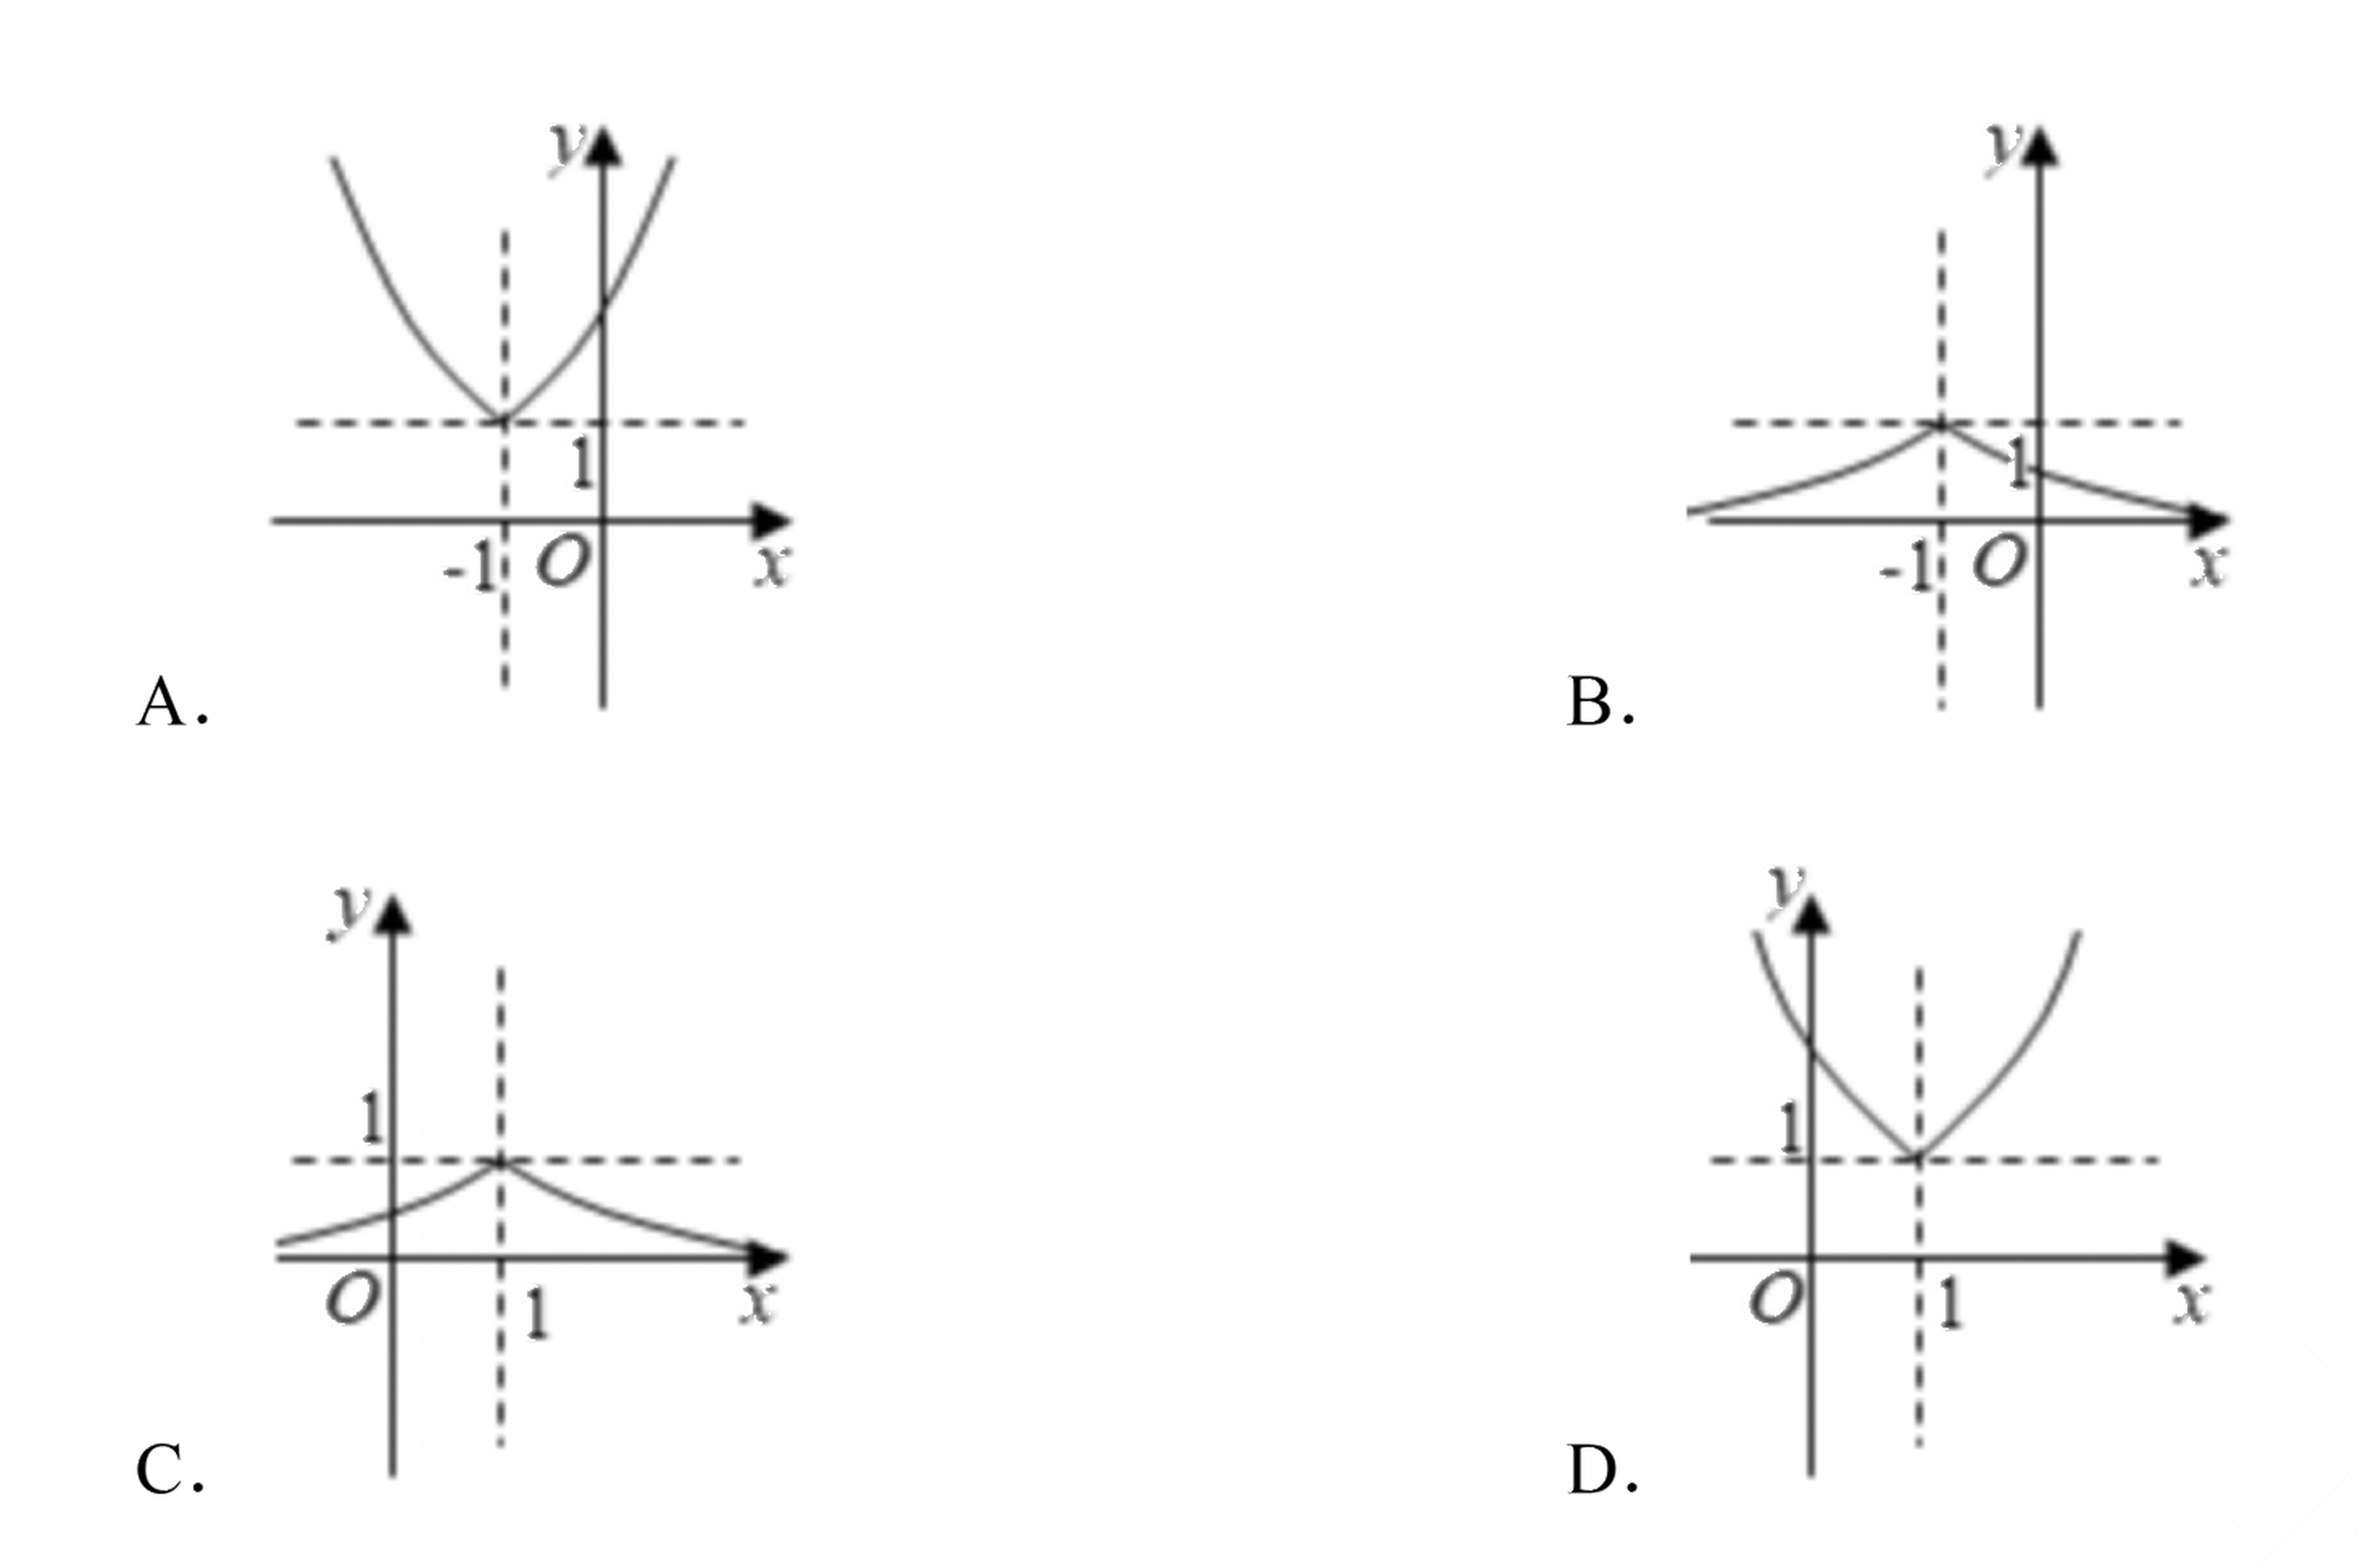
\includegraphics[width=0.80\textwidth]{figures/gao136_q22.png}
\end{center}

\ifanswer
\ans{$B$}
\fi

\end{enumerate}

\end{document}
"
% 紧凑版：xelatex "\def\iscompact{1}% 高一136_三林中学_期中.tex
%   —— 高一上数学"2026-2027 年三林中学高一上期中"（试卷版/答案版）
% 试卷版：xelatex 高一136_三林中学_期中.tex
% 答案版：xelatex "\def\isanswer{1}% 高一136_三林中学_期中.tex
%   —— 高一上数学"2026-2027 年三林中学高一上期中"（试卷版/答案版）
% 试卷版：xelatex 高一136_三林中学_期中.tex
% 答案版：xelatex "\def\isanswer{1}% 高一136_三林中学_期中.tex
%   —— 高一上数学"2026-2027 年三林中学高一上期中"（试卷版/答案版）
% 试卷版：xelatex 高一136_三林中学_期中.tex
% 答案版：xelatex "\def\isanswer{1}\input{高一136_三林中学_期中.tex}"
% 紧凑版：xelatex "\def\iscompact{1}\input{高一136_三林中学_期中.tex}"
%
% ① 原始材料：微信公众号"魔都数学加油站"文章，作者破晓，2026-11-15 18:04 发布；
% 连载"27学年高一136"，原文标题"27学年高一136——2026-2027年上海市三林中学高一上期中"；
% 原文链接：https://mp.weixin.qq.com/s/jaMzqMm6pDvcT0yM0d7eaQ。
% 正文为 7 张 PNG 页（01、04、06 为 4762x6735；02、03、05、07 为 2560x3620，
% 同一篇各页分辨率不同，逐页按各自分辨率裁图核对），题目下印有【答案】或【解析】，为讲评版。
% 题目、解析均据原图转录；卷面粉红色水印"魔都数学加油站"及公众号页脚未录入。
% 全卷 3 幅插图：第 13 题四幅坐标图选项（03 页）、第 20 题药物浓度折线/曲线图（05 页）、
% 第 22 题四幅抛物线/坐标图选项（07 页），均取原卷截图去粉色水印、去色、LANCZOS 放大，
% 四幅选项按原卷 2x2 排布合并为一张；图前按惯例加 \needvspace 守卫。
%
% 卷首标题：原卷印作"2026-2027 年三林中学高一上期中"（公众号标题中的"上海市"
% 卷面标题行没有，本稿照卷面），年份区间按全稿惯例排 en dash；原卷未印副标题，
% 本卷为期中卷、跨集合与常用逻辑用语／不等式／函数三章，按题目内容标为
% "集合与常用逻辑用语、不等式、函数"（与 125／126／128／129／131／132／133 同期中卷口径相同）：
% 集合与逻辑见 Q3、Q6、Q10、Q12、Q16、Q18、Q21，不等式见 Q5、Q7、Q8、Q9、Q14、Q15，
% 函数（幂函数、指数／对数、基本不等式应用）见 Q4、Q11、Q13、Q17、Q19、Q20、Q22。
%
% 题号体例：本卷共 20 题——一、填空题 3—12（10 题）、二、选择题 13—16（4 题）、
% 三、解答题 17—21（5 题）、四、附加题 22（1 题）。四节分别
% \setcounter{enumi}{2}／{12}／{16}／{21}。
%
% ② 与原卷的排版差异：
%   ① 原文从第 3 题起，本稿保留原题号；末节"四、附加题"另起 \bigsec，题号续到 22；
%   ② 原卷每题下直接印【答案】或【解析】，本稿按全稿惯例置于答案版；第 3、4、6 题只印
%      【答案】、无【解析】，提 \ans{}；第 14 题答案 C 印在题干括号内、无【解析】，按
%      高一53／高一108／高一132／高一133 成例括号留空、另提 \ans{$C$}；第 22 题答案 B
%      印在题干括号内、无【解析】，同例提 \ans{$B$}；第 13、15、16 题答案在解析末句
%      "故选 …"，括号内留空、不另提 \ans{}；其余各题印【解析】、无独立答案段；
%   ③ 原卷未印副标题，本稿按"知识模块"口径补出；
%   ④ 原卷填空横线按全稿惯例排为 \blankline[4.4em]；选择题括号排 \mbox{（\quad）}、
%      每个选项段前按惯例加 \keepwithprev（四幅图选项那一枚放在 \begin{center} 之前）；
%      解答题不留作答区、不加 \anspace（原卷为讲评版，与 129／131／132／133 同）；
%   ⑤ 原卷数集排斜体 $R$／$R^+$／$Z$，按全稿惯例改 \R／\R^+／\Z；空集记号 \varnothing；
%      绝对值排 \lvert…\rvert，集合描述竖线排 \mid；不等号按全稿惯例排 \leqslant／\geqslant；
%   ⑥ 子题标号 (1)(2)(3) 原卷用半角括号，照录；圈数字 ①②③④ 照录；第 12 题甲／乙／丙
%      三行与第 14 题四个编号不等式照录；
%   ⑦ 数学式内半角逗号照录（如 Q4"$a>0,a\neq1$"、Q6"$\{(-2,4),(1,1)\}$"、
%      Q7"$a=2+3=5,b=2\times3=6$"、Q11"$x_1,x_2$"、Q12"$m,n\in R^+$"、
%      Q15"$a>1,b\geq0$"、Q18"$B=(2a,a+1)$"、Q20"$4t,0\leq t\leq1$"、
%      Q21"$\{-3,-2,-1,0,1,2,3\}$"）；原卷行末西文句点照录，行中全角逗号照录；
%   ⑧ 三幅插图：第 13 题四幅坐标图选项合并裁为一张 \includegraphics（题前 \needvspace{9cm}）；
%      第 20 题折线/曲线图取 05 页截图（0.42\textwidth）；第 22 题四幅抛物线/坐标图选项合并
%      裁为一张（题前 \needvspace{9cm}）。第 13、22 题分别是"二、选择题""四、附加题"的首题
%      且带大图块，另在两处 \bigsec 之前各加 \needvspace{11cm} 连节标题一起量，避免节标题
%      孤立在页末（切页审计 B 类；照 高一26／40／59 成例）。第 20 题图不是节首题、三版试排
%      图均与题干同页，加 7cm 守卫反会多出一张只有两行正文的稀疏页，故不另加守卫；
%      三版切页审计均"合计异常：无"（试卷 4 页／紧凑 4 页／答案 6 页）；
%   ⑨ 跨页续印按题合并：Q16 题干在 03 页、括号与选项及【解析】在 04 页；Q19 题干在 04 页、
%      (2) 与【解析】在 05 页；Q20 (3)【解析】在 06 页；Q22 四幅图在 07 页；本稿按题连排；
%   ⑩ 题干中的中文弯引号按原卷照录，注释内一律 ASCII 引号；原卷"图像／图象"两种写法混用，
%      逐处照录（Q4、Q19 作"图像"，Q13、Q15、Q20、Q22 作"图象"）；
%   ⑪ 附加题节：原卷印"四、附加题"，本稿用 \bigsec{四、附加题} 另起一节、
%      \setcounter{enumi}{21}，顶层 1 个 \item（与 高一09／15／16／22／35／39／47／61 同口径）；
%      Q22 只印括号内答案、提 \ans{}，不计入 \step 账。
%
% 判别式字形：全卷仅第 9 题【解析】cases 块出现判别式"$\Delta=a^2-8a<0$"，原卷印
%   等腰、偏高的三角 $\Delta$，逐处放大核对并照录 \Delta；全卷未出现扁等边三角 \triangle。
%
% 子集符号：第 18 题 (2) 题干"$B\subseteq A$"与【解析】"$B\subseteq A$"两处原卷均印
%   带下划线 $\subseteq$，逐处放大核对、照录 \subseteq；全卷未出现单线 \subset。
%
% 原卷存疑照录（均照录未改，正文对应处另有 % 注）：
%   第 12 题乙行"$\dfrac{m+n}{mm}=\dfrac1{mn}$"前一分母印作 $mm$（后一处作 $mn$），照录；
%   第 12 题【解析】"$\geqslant\dfrac1{100}\left[a^2+1+2\sqrt{a^2}\right]$"保留 $\sqrt{a^2}$
%      未化简为 $a$，照录；
%   第 13 题【解析】"排除 BC"与"排除 D"连写选项字母，照录；
%   第 18 题 (2)【解析】末行"所以实数 $a$ 的取值范围 $(-\infty,-2]\cup[\frac12,1)$"
%      "取值范围"后脱"是／为"字，照录；
%   第 21 题 (3) 题干"求出使得集合 $B$ 中元素最少的 $k$ 的所有取值"而【解析】只给出
%      $k=-2$ 一处，措辞照录。
%
% 行数复核：逐题数 \step 条数，合计 51 条（Q3：0；Q4：0；Q5：2；Q6：0；Q7：2；Q8：1；
% Q9：1；Q10：4；Q11：1；Q12：4；Q13：2；Q14：0；Q15：2；Q16：3；Q17：1；Q18：5；
% Q19：4；Q20：7；Q21：12；Q22：0），与原卷印刷行逐题相等（cases 块作一个印刷行计）。
% 第 3、4、6、14、22 题只印【答案】、提 \ans{}，不计入 \step 账；第 13、15、16 题答案在
% 解析末句，括号内留空、不另提 \ans{}。
%
\documentclass[a4paper,11pt]{article}
\usepackage{common}

\begin{document}

\examtitlest[3]{2026--2027 年三林中学高一上期中}{集合与常用逻辑用语、不等式、函数}

\bigsec{一、填空题}

\begin{enumerate}
\setcounter{enumi}{2}

\item 用反证法证明命题“若 $x+y\neq5$，则 $x\neq2$ 或 $y\neq3$”为真命题时，第一个步骤是\blankline[4.4em].

\ifanswer
\ans{假设 $x=2$ 且 $y=3$}
\fi

\item 函数 $y=a^{x-1}+1(a>0,a\neq1)$ 的图像恒过定点 $A$，则点的坐标是\blankline[4.4em].

\ifanswer
\ans{$(1,2)$}
\fi

\item 已知 $x>1$，则 $x+\dfrac4{x-1}$ 的最小值是\blankline[4.4em].

\ifanswer
\solbegin
\step{由 $x>1$，得 $x-1>0$，则 $x+\dfrac4{x-1}=x-1+\dfrac4{x-1}+1\geqslant2\sqrt{(x-1)\cdot\dfrac4{x-1}}+1=5$，}
\step{当且仅当 $x-1=\dfrac4{x-1}$ 即 $x=3$ 时取等号，取得最小值 $5$.}
\solend
\fi

\item 已知集合 $A=\{(x,y)\mid y=x^2\}$，集合 $B=\{(x,y)\mid y=2-x\}$，求 $A\cap B=$\blankline[4.4em].

\ifanswer
\ans{$\{(-2,4),(1,1)\}$}
\fi

\item 已知一元二次不等式 $x^2-ax+b<0$ 的解集为 $(2,3)$，则不等式 $bx^2-ax+1>0$ 的解集是\blankline[4.4em].

\ifanswer
\solbegin
\step{$a=2+3=5,b=2\times3=6$，则 $bx^2-ax+1>0$ 即 $6x^2-5x+1>0$，}
\step{即 $(3x-1)(2x-1)>0$，解集为 $\left(-\infty,\dfrac13\right)\cup\left(\dfrac12,+\infty\right)$.}
\solend
\fi

\item 不等式 $(x+2)^3<(5-2x)^3$ 的解集为\blankline[4.4em].

\ifanswer
\solbegin
\step{由 $(x+2)^3<(5-2x)^3$ 得 $x+2<5-2x$，故解集为 $(-\infty,1)$.}
\solend
\fi

\item 若关于 $x$ 的不等式 $ax^2-ax+2>0$ 的解集为 $\R$，则实数 $a$ 的取值范围是\blankline[4.4em].

\ifanswer
\solbegin
\step{由题意得 $a=0$ 或 $\begin{cases}a>0\\\Delta=a^2-8a<0\end{cases}$，所以 $0\leqslant a<8$.}% 判别式原卷印高三角 $\Delta$，照录
\solend
\fi

\item 已知关于 $x$ 的不等式 $\lvert x+3\rvert+\lvert x-a\rvert\geqslant5$ 恒成立，则实数 $a$ 的取值范围为\blankline[4.4em].

\ifanswer
\solbegin
\step{因为 $\lvert x+3\rvert+\lvert x-a\rvert\geqslant\lvert x-a-x-3\rvert=\lvert 3+a\rvert$，}
\step{要使 $\lvert x+3\rvert+\lvert x-a\rvert\geqslant5$ 恒成立，则 $\lvert a+3\rvert\geqslant5$ 即可，}
\step{所以 $a+3\geqslant5$ 或 $a+3\leqslant-5$，解得 $a\geqslant2$ 或 $a\leqslant-8$，}
\step{即实数 $a$ 的取值范围是 $(-\infty,-8]\cup[2,+\infty)$.}
\solend
\fi

\item 若方程 $\lg^2 x-2\lg x-2=0$ 的两个解为 $x_1,x_2$，求 $\log_{x_1}x_2+\log_{x_2}x_1$ 的值为\blankline[4.4em].

\ifanswer
\solbegin
\step{$\log_{x_1}x_2+\log_{x_2}x_1=\dfrac{\lg x_2}{\lg x_1}+\dfrac{\lg x_1}{\lg x_2}=\dfrac{(\lg x_1+\lg x_2)^2-2\lg x_1\lg x_2}{\lg x_1\lg x_2}=-4$.}
\solend
\fi

\item 三个同学对问题“已知 $m,n\in \R^+$，且 $m+n=1$，求 $\dfrac1m+\dfrac1n$ 的最小值”提出各自的解题思路：

思路：

甲：$\dfrac1m+\dfrac1n=\dfrac{m+n}{m}+\dfrac{m+n}{n}=2+\dfrac nm+\dfrac mn$，可用基本不等式求解；

乙：$\dfrac1m+\dfrac1n=\dfrac{m+n}{mm}=\dfrac1{mn}=\dfrac1{m(1-m)}$，可用二次函数配方法求解；% 原卷前一分母印作 $mm$，照录

丙：$\dfrac1m+\dfrac1n=\left(\dfrac1m+\dfrac1n\right)(m+n)=2+\dfrac nm+\dfrac mn$，可用基本不等式求解；参考上述解题思路，

可求得当 $x=$\blankline[4.4em]时，$y=\dfrac{a^2}{x^2}+\dfrac1{100-x^2}$（$0<x<10$，$a>0$）有最小值.

\ifanswer
\solbegin
\step{$y=\dfrac{a^2}{x^2}+\dfrac1{100-x^2}=\left(\dfrac{a^2}{x^2}+\dfrac1{100-x^2}\right)[x^2+(100-x^2)]\times\dfrac1{100}$}
\step{$=\dfrac1{100}\left[a^2+1+\dfrac{x^2}{100-x^2}+\dfrac{a^2(100-x^2)}{x^2}\right]\geqslant\dfrac1{100}\left[a^2+1+2\sqrt{a^2}\right]$}% 原卷保留 $\sqrt{a^2}$ 未化简，照录
\step{当且仅当 $\dfrac{x^2}{100-x^2}=\dfrac{a^2(100-x^2)}{x^2}$，即 $x=\sqrt{\dfrac{100a}{a+1}}$ 时，}
\step{$y=\dfrac{a^2}{x^2}+\dfrac1{100-x^2}(0<x<10,a>0)$ 有最小值.}
\solend
\fi

\end{enumerate}

% 第 13 题是"二、选择题"首题且带 9cm 图块，守卫须放在 \bigsec 之前连节标题一起量，
% 否则"二、选择题"会孤立在页末（B 类，照 高一26／40／59 成例）
\needvspace{11cm}
\bigsec{二、选择题}

\begin{enumerate}
\setcounter{enumi}{12}

% 第 13 题四幅坐标图选项是一整块，守卫放在 \item 之前
\needvspace{9cm}
\item 下列图象中，最符合函数 $y=x^{\frac54}$ 的图象的是\mbox{（\quad）}

\keepwithprev
\begin{center}
% 四幅坐标图选项取原卷 03 页截图去粉色水印，按原卷 2x2 排布合并为一张
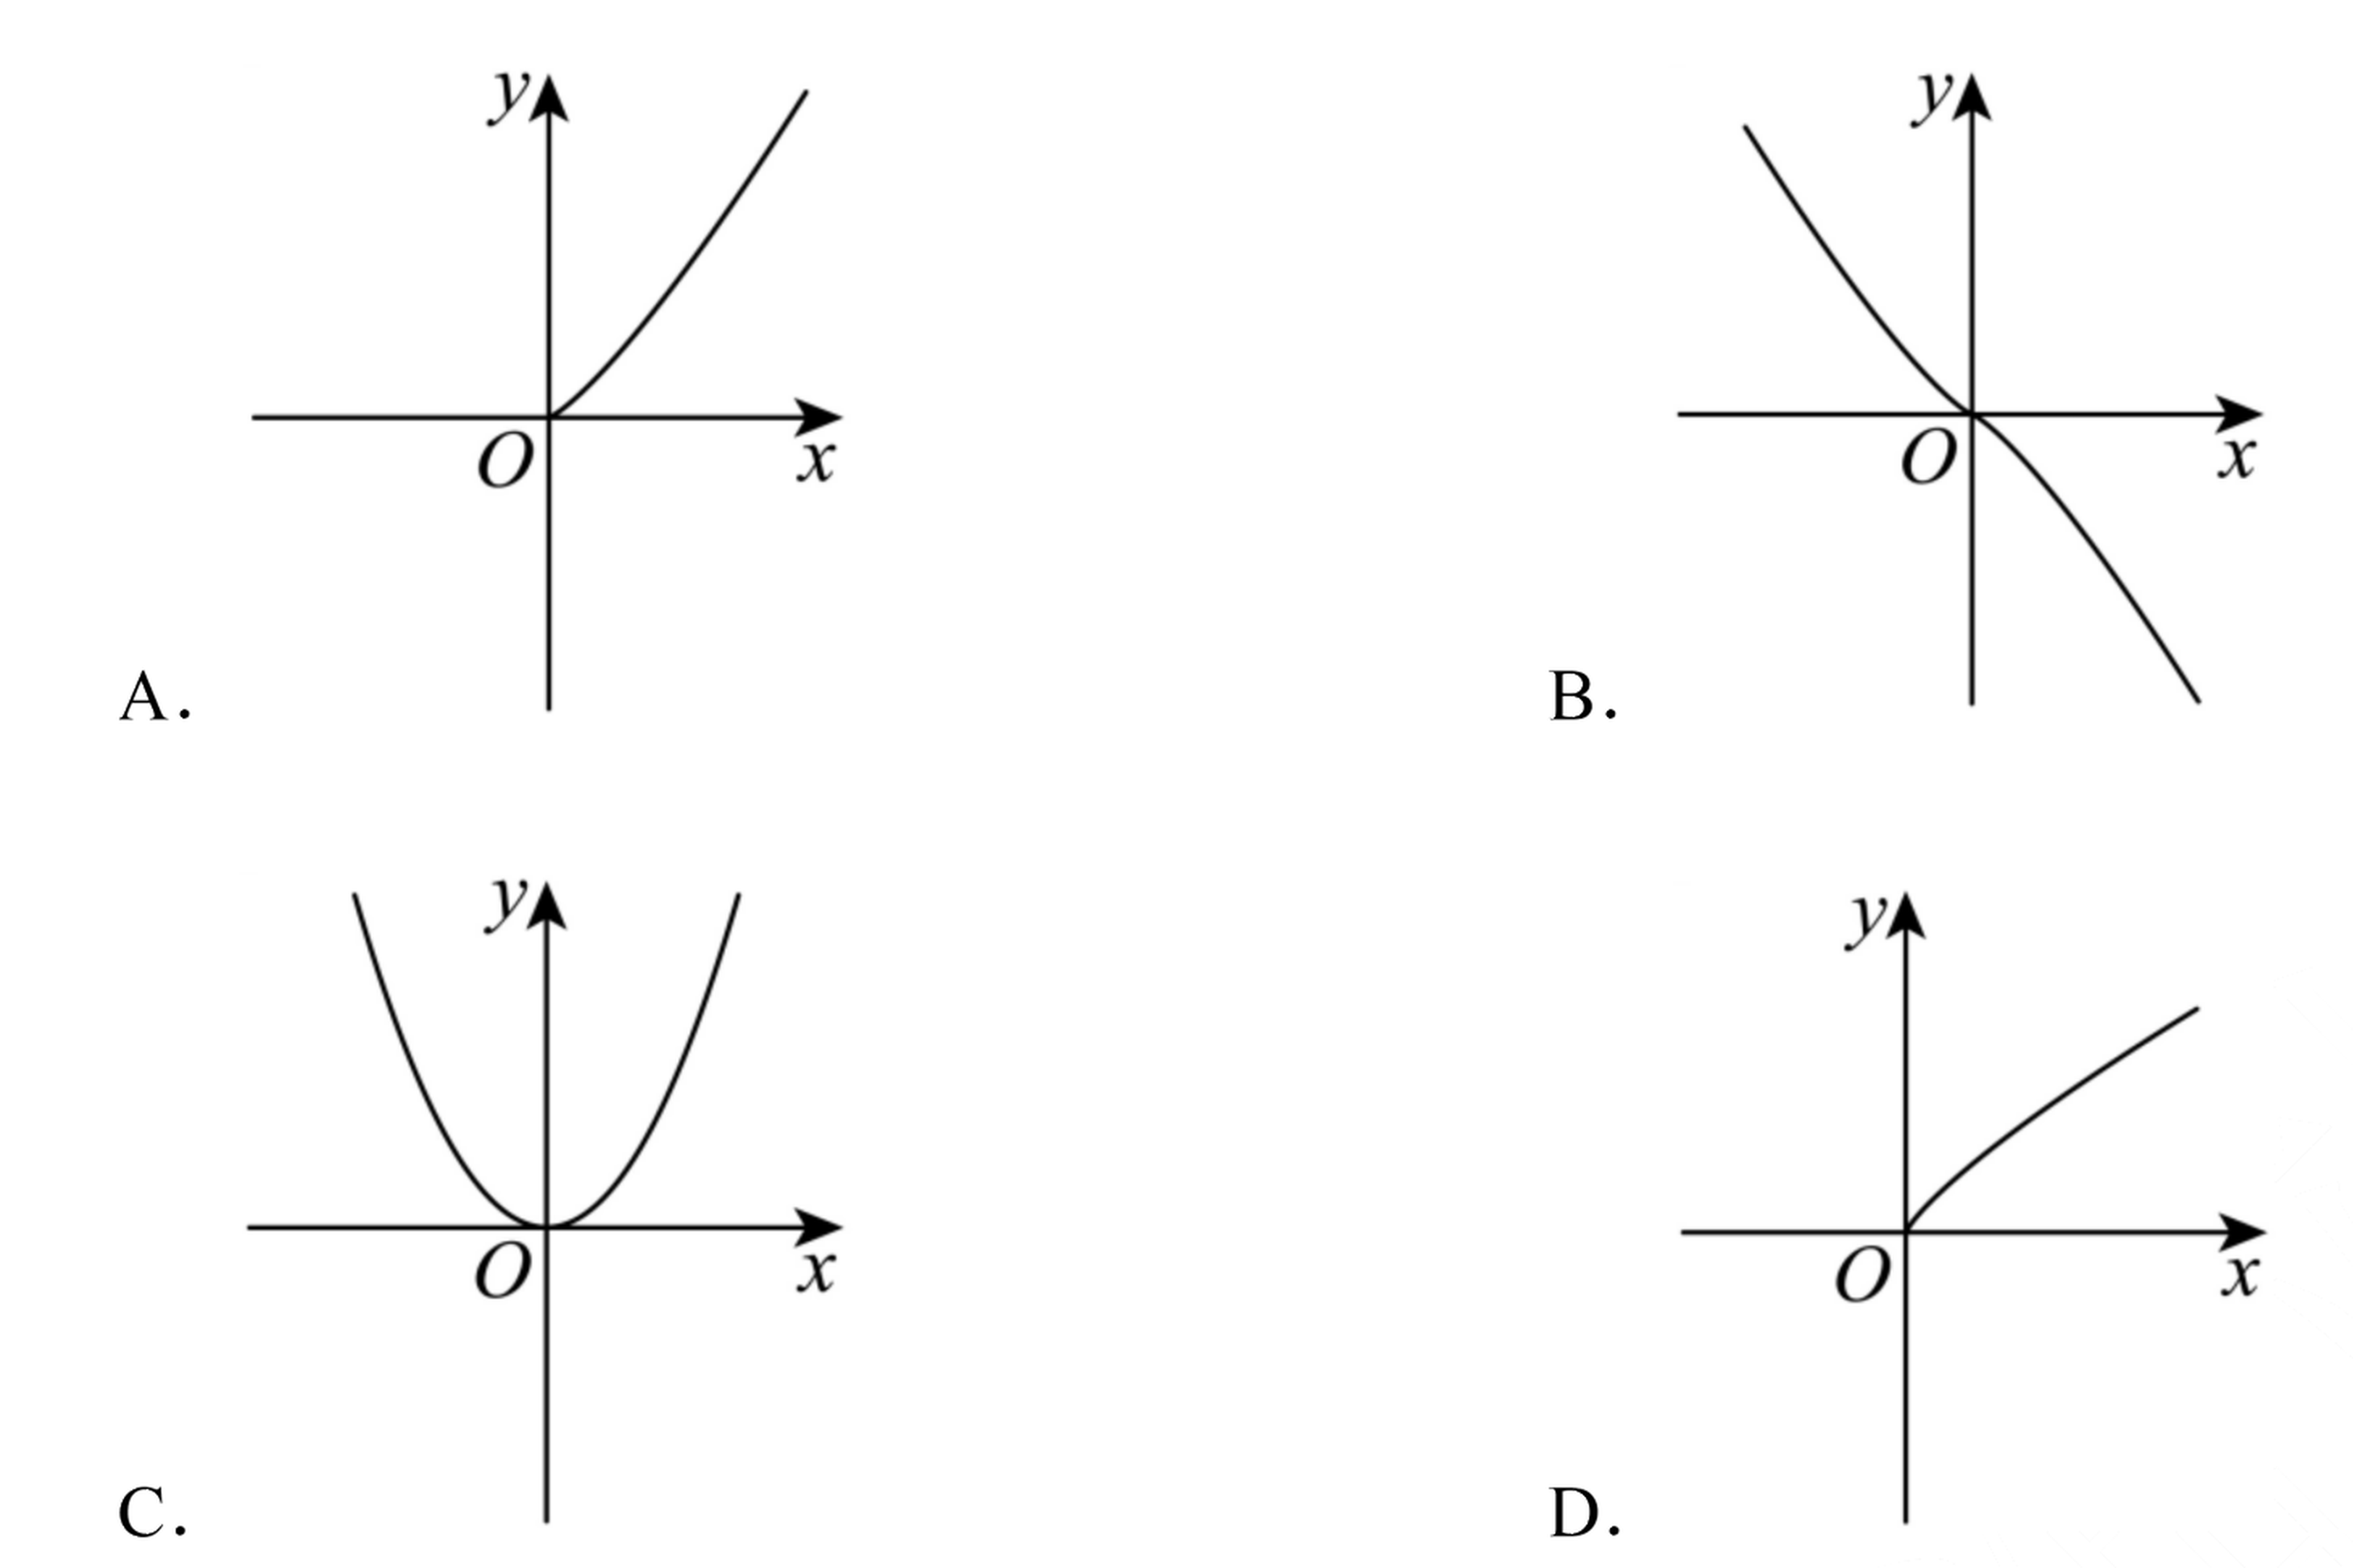
\includegraphics[width=0.80\textwidth]{figures/gao136_q13.png}
\end{center}

\ifanswer
\solbegin
\step{由 $y=x^{\frac54}=\sqrt[4]{x^5}$，函数的定义域为 $[0,+\infty)$，排除 BC，}% 原卷"排除 BC"连写，照录
\step{因为 $\dfrac54>1$，所以函数 $y=x^{\frac54}$ 的图象呈现下凸的趋势，排除 D. 故选 $A$.}
\solend
\fi

\item 下列不等式① $a+\dfrac1a\geqslant2$；② $a^2+4\geqslant4a$；③ $\left\lvert\dfrac ba+\dfrac ab\right\rvert\geqslant2$；④ $\dfrac{2a^2b^2}{a^2+b^2}\leqslant ab$；其中恒成立的是\mbox{（\quad）}

\keepwithprev
A. ①④\qquad B. ③④\qquad C. ②③\qquad D. ①②

\ifanswer
\ans{$C$}
\fi

\item 函数 $y=a^x+b-1(a>0,a\neq1)$ 单调递增且图象不经过第四象限，则 $a,b$ 满足的条件为\mbox{（\quad）}

\keepwithprev
A. $a>1,b\leqslant1$\qquad B. $a>1,b\geqslant0$\qquad C. $0<a<1,b\leqslant1$\qquad D. $0<a<1,b\geqslant1$

\ifanswer
\solbegin
\step{因为函数 $y=a^x+b-1$ 单调递增，所以 $a>1$，}
\step{图象不经过第四象限，则 $x=0$ 时，$y=b\geqslant0$，所以 $a>1,b\geqslant0$，故选 $B$.}
\solend
\fi

\item 设关于 $x$ 的不等式 $\dfrac{ax-1}{x^2-a}<0$ 的解集为 $S$，且 $3\in S$，$4\notin S$，则实数 $a$ 的取值范围为\mbox{（\quad）}

\keepwithprev
A. $(-\infty,-\sqrt3)\cup\left(\dfrac13,\sqrt3\right)$\qquad B. $\left(-\infty,\dfrac14\right)\cup(16,+\infty)$

C. $\left[\dfrac14,\dfrac13\right)\cup(9,16]$\qquad D. 不能确定

\ifanswer
\solbegin
\step{若 $3\in S$，则 $\dfrac{3a-1}{9-a}<0$，解得 $a\in\left(-\infty,\dfrac13\right)\cup(9,+\infty)$，}
\step{若 $4\notin S$，则 $16-a=0$ 或 $\dfrac{4a-1}{16-a}\geqslant0$，解得 $a\in\left[\dfrac14,16\right]$，}
\step{故实数 $a$ 的取值范围为 $\left[\dfrac14,\dfrac13\right)\cup(9,16]$，故选 $C$.}
\solend
\fi

\end{enumerate}

\bigsec{三、解答题}

\begin{enumerate}
\setcounter{enumi}{16}

\item 计算：(1) 计算 $\dfrac{\lg8+\lg125-\lg2-\lg5}{\lg\sqrt{10}\cdot\lg0.1}$；(2) 若 $a^{2x}=2(a>0)$，求 $\dfrac{a^{3x}+a^{-3x}}{a^x+a^{-x}}$.

\ifanswer
\solbegin
\step{(1) 原式 $=\dfrac{2-1}{\frac12\cdot(-1)}=-2$；(2) 原式 $=a^{2x}-1+a^{-2x}=2-1+\dfrac12=\dfrac32$.}
\solend
\fi

\item 不等式 $\dfrac{x-1}{x+1}\geqslant0$ 的解集为 $A$，不等式 $(x-a-1)(2a-x)>0(a<1)$ 的解集为 $B$.

(1) 求集合 $A$；

(2) 若 $B\subseteq A$，求实数 $a$ 的取值范围.

\ifanswer
\solbegin
\step{(1) $A=(-\infty,-1)\cup[1,+\infty)$.}
\step{(2) 由 $(x-a-1)(2a-x)>0(a<1)$，得 $(x-a-1)(x-2a)<0(a<1)$，}
\step{因为 $a<1$，所以 $a+1>2a$，所以 $B=(2a,a+1)$，}
\step{因为 $B\subseteq A$，所以 $2a\geqslant1$ 或 $a+1\leqslant-1$，即 $a\geqslant\dfrac12$ 或 $a\leqslant-2$，}
\step{而 $a<1$，所以实数 $a$ 的取值范围 $(-\infty,-2]\cup\left[\dfrac12,1\right)$.}% 原卷"取值范围"后脱"是／为"，照录
\solend
\fi

\item 已知幂函数 $y=x^m(m\in\R)$ 经过点 $\left(4,\dfrac12\right)$.

(1) 求此幂函数的表达式和定义域；

(2) 已知点 $A(a+2,y_1)$，点 $B(3-2a,y_2)(a\in\R)$ 在此幂函数的图像上，且满足 $y_1<y_2$，求实数 $a$ 的取值范围.

\ifanswer
\solbegin
\step{(1) 幂函数 $y=x^m(m\in\R)$ 经过点 $\left(4,\dfrac12\right)$，所以 $4^m=\dfrac12\Rightarrow m=-\dfrac12$，}
\step{所以 $f(x)=x^{-\frac12}$，定义域为 $(0,+\infty)$.}
\step{(2) 由于函数 $f(x)$ 在其定义域 $(0,+\infty)$ 上严格减，}
\step{由 $y_1<y_2$，得 $a+2>3-2a\geqslant0\Rightarrow a\in\left(\dfrac13,\dfrac32\right]$.}
\solend
\fi

% 第 20 题图取 05 页截图（0.42\textwidth、高约 6cm）。试排 \item 前加 7cm 守卫会多出
% 一张只有两行正文的稀疏页，且三版不加守卫时图均与题干、【解析】同页，故不另加守卫
\item 某医药研究所开发一种抗甲流新药，如果成年人按规定的剂量服用，据监测：服药后每毫升血液中的含药量 $y$（微克）与时间 $t$（小时）之间近似满足如图所示的曲线.

(1) 结合图，求 $k$ 与 $a$ 的值；

(2) 写出服药后 $y$ 与 $t$ 之间的函数关系式 $y=f(t)$；

(3) 据进一步测定：每毫升血液中含药量不少于 $0.5$ 微克时治疗疾病有效，求服药一次治疗有效的时间范围？

\begin{center}
% 图取原卷 05 页截图去粉色水印、去色，3x LANCZOS 放大
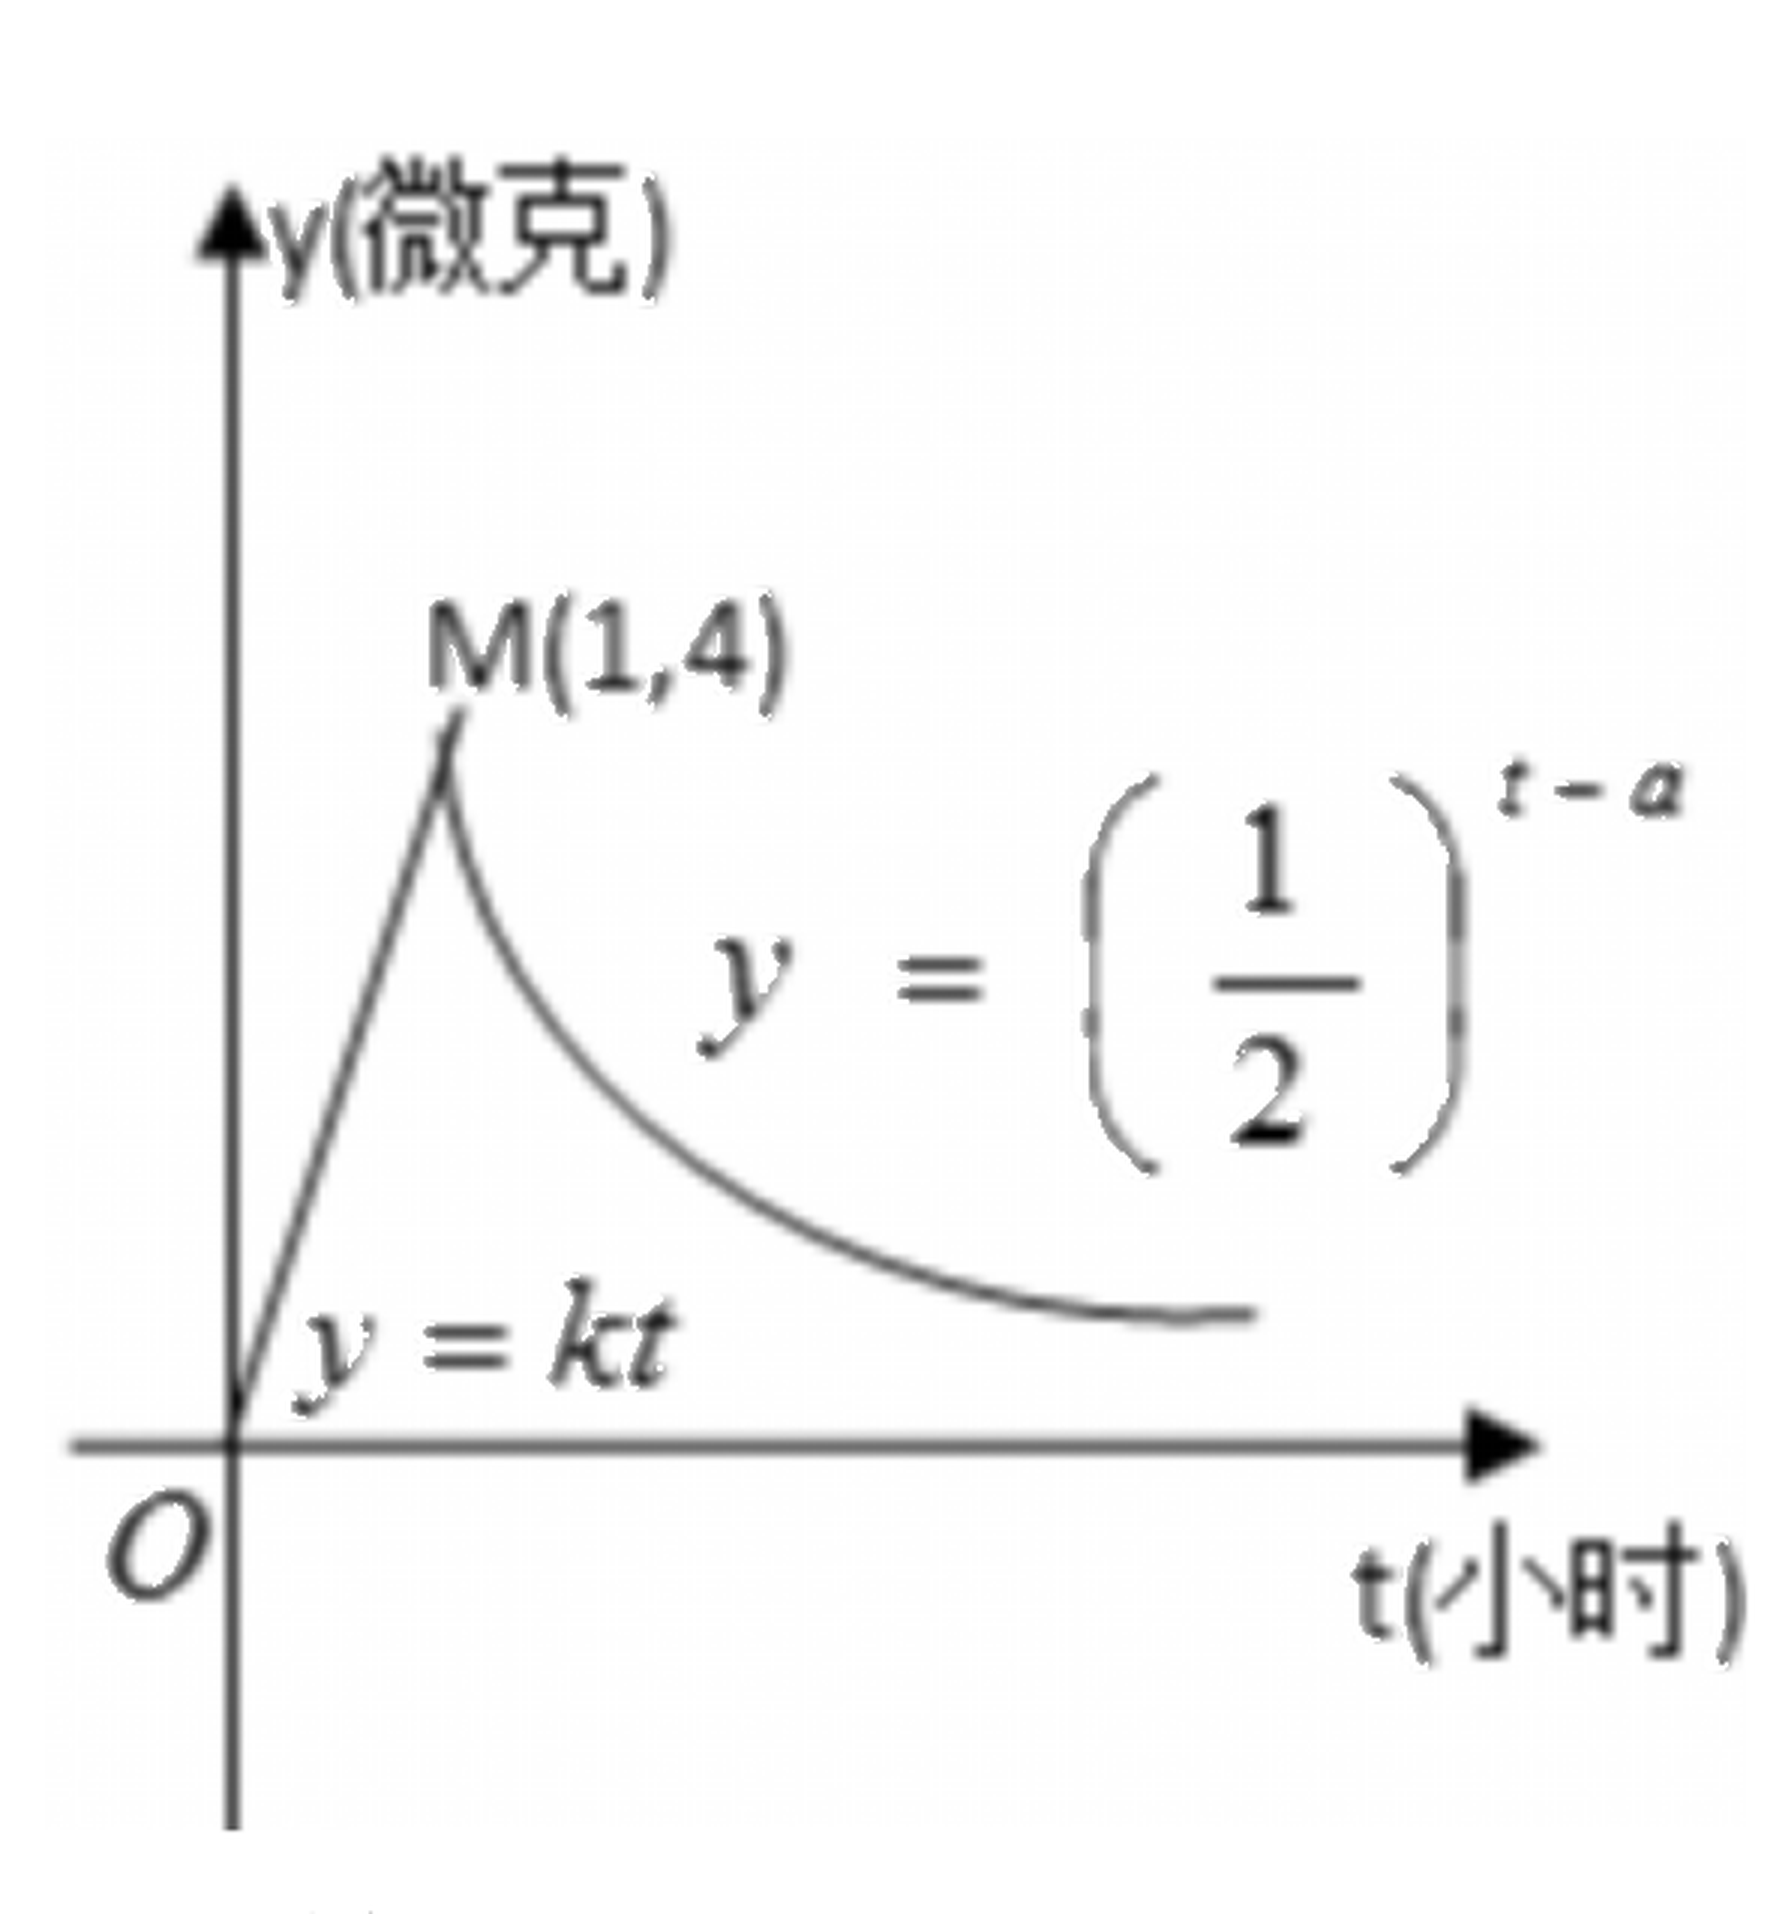
\includegraphics[width=0.42\textwidth]{figures/gao136_q20.png}
\end{center}

\ifanswer
\solbegin
\step{(1) 当 $0\leqslant t\leqslant1$ 时，函数图象是一条线段，由于过原点与点 $(1,4)$，所以 $k=4$，}
\step{其解析式为 $y=4t$，$0\leqslant t\leqslant1$；}
\step{当 $t\geqslant1$ 时，函数的解析式为 $y=\left(\dfrac12\right)^{t-a}$，}
\step{此时 $M(1,4)$ 在曲线上，将此点的坐标代入函数解析式得 $4=\left(\dfrac12\right)^{1-a}$，}
\step{解得 $a=3$；}
\step{(2) 由 (1) 得 $f(t)=\begin{cases}4t,0\leqslant t\leqslant1\\\left(\frac12\right)^{t-3},t>1\end{cases}$；}
\step{(3) 由 (2) 得，令 $f(t)\geqslant0.5$，即 $\begin{cases}4t\geqslant0.5,0\leqslant t\leqslant1\\\left(\frac12\right)^{t-3}\geqslant0.5,t>1\end{cases}$，所以 $\dfrac18\leqslant t\leqslant4$.}
\solend
\fi

\item 已知关于 $x$ 的不等式 $(kx-k^2-4)(x-4)>0$，其中 $k\in\R$.

(1) 当 $k=-1$，求不等式的解集 $A$；

(2) 当 $k$ 变化时，试求不等式的解集 $A$；

(3) 对于不等式解集 $A$，满足 $A\cap\Z=B$. 试探究集合 $B$ 能否为有限集，若能，求出使得集合 $B$ 中元素最少的 $k$ 的所有取值，并用列举法表示此时的集合 $B$，若不能，说明理由；

\ifanswer
\solbegin
\step{(1) 当 $k=-1$ 时，原不等式可化为 $(x+5)(x-4)<0$，}
\step{解得 $-5<x<4$，故不等式的解集为 $\{x\mid -5<x<4\}$；}
\step{(2) 当 $k=0$ 时，解集为 $\{x\mid x<4\}$，}
\step{当 $k>0$ 时，$\dfrac{k^2+4}{k}=k+\dfrac4k\geqslant4$，解集为 $\{x\mid x<4\text{ 或 }x>\dfrac{k^2+4}{k}\}$；}
\step{当 $k<0$ 时，解集为 $\{x\mid \dfrac{k^2+4}{k}<x<4\}$，}
\step{综上，当 $k=0$ 时，$A=\{x\mid x<4\}$，}
\step{当 $k>0$ 时，$A=\{x\mid x<4\text{ 或 }x>\dfrac{k^2+4}{k}\}$；}
\step{当 $k<0$ 时，$A=\{x\mid \dfrac{k^2+4}{k}<x<4\}$，}
\step{(3) 由 (2) 得当 $k\geqslant0$ 时，$B$ 为无限集，当 $k<0$ 时，$B$ 为有限集，}
\step{此时，$\dfrac{k^2+4}{k}=k+\dfrac4k\leqslant-4$，当且仅当 $k=-2$ 时取等号，}
\step{所以 $k=-2$ 时，$B$ 中元素最少，此时 $A=\{x\mid -4<x<4\}$，}
\step{所以 $B=\{-3,-2,-1,0,1,2,3\}$.}
\solend
\fi

\end{enumerate}

% 第 22 题是"四、附加题"首题且带 9cm 图块，守卫须放在 \bigsec 之前连节标题一起量，
% 否则"四、附加题"会孤立在页末（B 类，照 高一26／40／59 成例）
\needvspace{11cm}
\bigsec{四、附加题}

\begin{enumerate}
\setcounter{enumi}{21}

% 第 22 题四幅抛物线/坐标图选项是一整块，守卫放在 \item 之前
\needvspace{9cm}
\item 函数 $f(x)=\left(\dfrac12\right)^{\lvert x+1\rvert}$ 的图象大致为\mbox{（\quad）}

\keepwithprev
\begin{center}
% 四幅抛物线/坐标图选项取原卷 07 页截图去粉色水印，按原卷 2x2 排布合并为一张
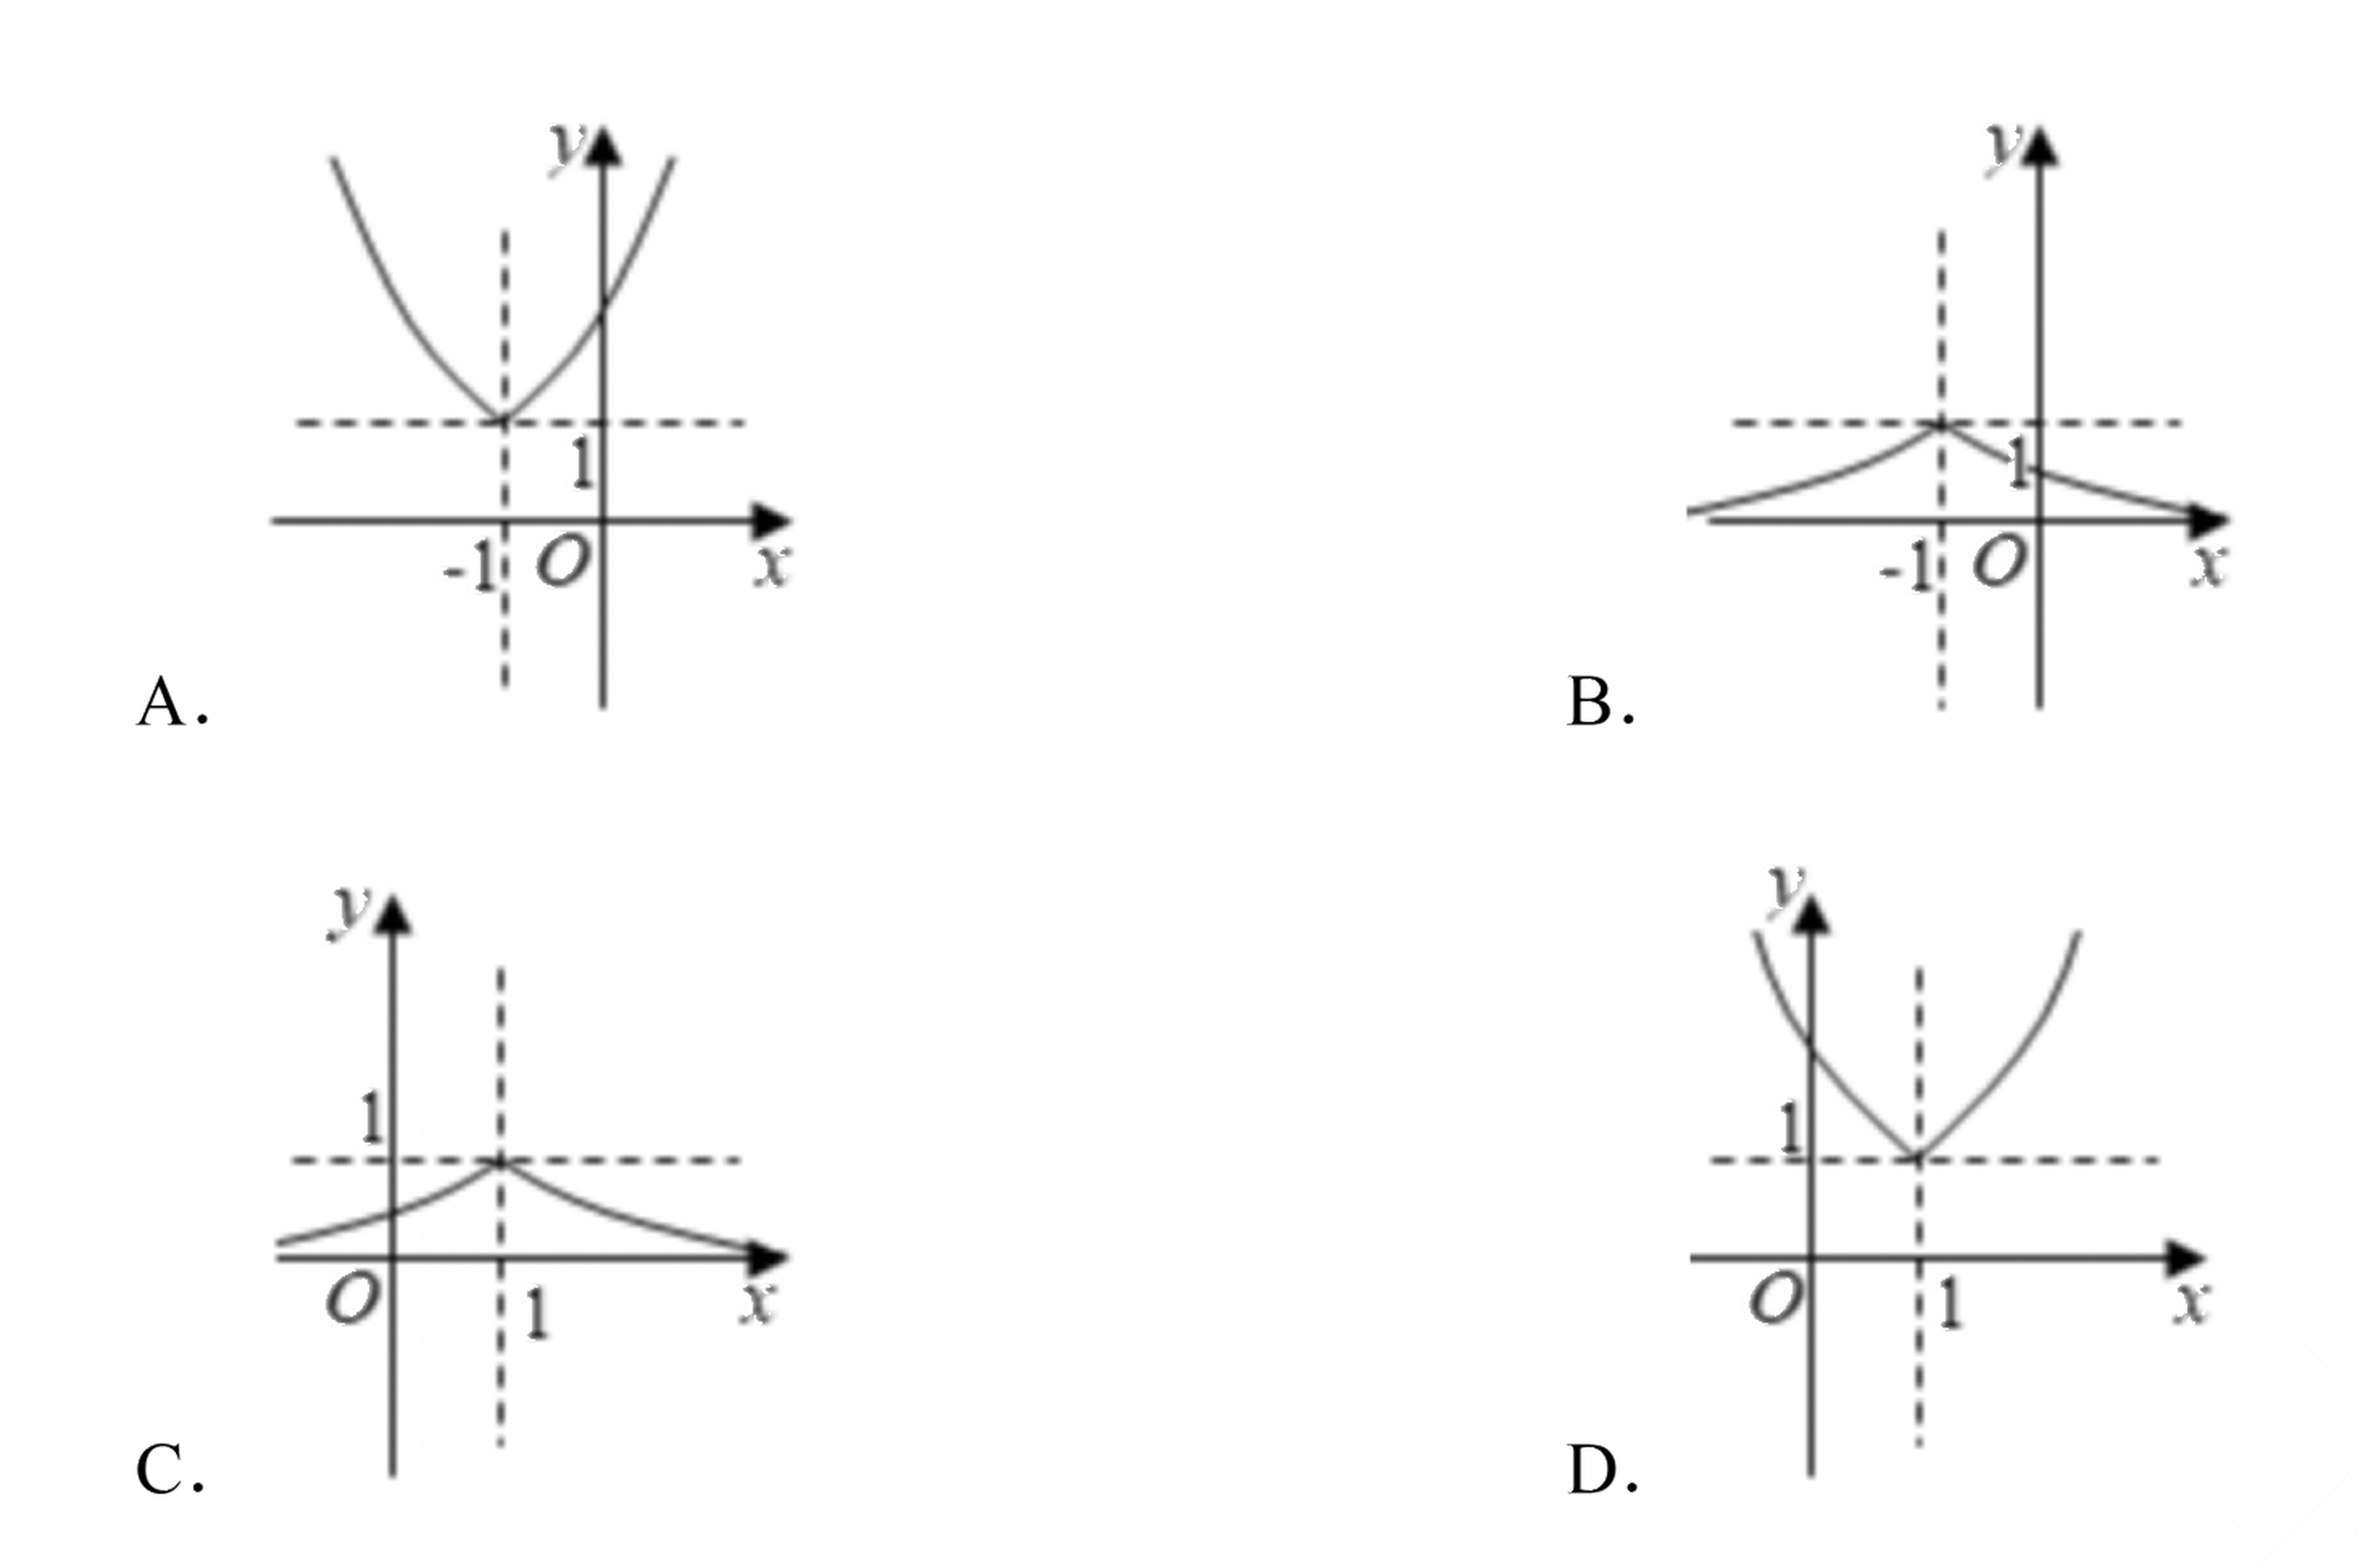
\includegraphics[width=0.80\textwidth]{figures/gao136_q22.png}
\end{center}

\ifanswer
\ans{$B$}
\fi

\end{enumerate}

\end{document}
"
% 紧凑版：xelatex "\def\iscompact{1}% 高一136_三林中学_期中.tex
%   —— 高一上数学"2026-2027 年三林中学高一上期中"（试卷版/答案版）
% 试卷版：xelatex 高一136_三林中学_期中.tex
% 答案版：xelatex "\def\isanswer{1}\input{高一136_三林中学_期中.tex}"
% 紧凑版：xelatex "\def\iscompact{1}\input{高一136_三林中学_期中.tex}"
%
% ① 原始材料：微信公众号"魔都数学加油站"文章，作者破晓，2026-11-15 18:04 发布；
% 连载"27学年高一136"，原文标题"27学年高一136——2026-2027年上海市三林中学高一上期中"；
% 原文链接：https://mp.weixin.qq.com/s/jaMzqMm6pDvcT0yM0d7eaQ。
% 正文为 7 张 PNG 页（01、04、06 为 4762x6735；02、03、05、07 为 2560x3620，
% 同一篇各页分辨率不同，逐页按各自分辨率裁图核对），题目下印有【答案】或【解析】，为讲评版。
% 题目、解析均据原图转录；卷面粉红色水印"魔都数学加油站"及公众号页脚未录入。
% 全卷 3 幅插图：第 13 题四幅坐标图选项（03 页）、第 20 题药物浓度折线/曲线图（05 页）、
% 第 22 题四幅抛物线/坐标图选项（07 页），均取原卷截图去粉色水印、去色、LANCZOS 放大，
% 四幅选项按原卷 2x2 排布合并为一张；图前按惯例加 \needvspace 守卫。
%
% 卷首标题：原卷印作"2026-2027 年三林中学高一上期中"（公众号标题中的"上海市"
% 卷面标题行没有，本稿照卷面），年份区间按全稿惯例排 en dash；原卷未印副标题，
% 本卷为期中卷、跨集合与常用逻辑用语／不等式／函数三章，按题目内容标为
% "集合与常用逻辑用语、不等式、函数"（与 125／126／128／129／131／132／133 同期中卷口径相同）：
% 集合与逻辑见 Q3、Q6、Q10、Q12、Q16、Q18、Q21，不等式见 Q5、Q7、Q8、Q9、Q14、Q15，
% 函数（幂函数、指数／对数、基本不等式应用）见 Q4、Q11、Q13、Q17、Q19、Q20、Q22。
%
% 题号体例：本卷共 20 题——一、填空题 3—12（10 题）、二、选择题 13—16（4 题）、
% 三、解答题 17—21（5 题）、四、附加题 22（1 题）。四节分别
% \setcounter{enumi}{2}／{12}／{16}／{21}。
%
% ② 与原卷的排版差异：
%   ① 原文从第 3 题起，本稿保留原题号；末节"四、附加题"另起 \bigsec，题号续到 22；
%   ② 原卷每题下直接印【答案】或【解析】，本稿按全稿惯例置于答案版；第 3、4、6 题只印
%      【答案】、无【解析】，提 \ans{}；第 14 题答案 C 印在题干括号内、无【解析】，按
%      高一53／高一108／高一132／高一133 成例括号留空、另提 \ans{$C$}；第 22 题答案 B
%      印在题干括号内、无【解析】，同例提 \ans{$B$}；第 13、15、16 题答案在解析末句
%      "故选 …"，括号内留空、不另提 \ans{}；其余各题印【解析】、无独立答案段；
%   ③ 原卷未印副标题，本稿按"知识模块"口径补出；
%   ④ 原卷填空横线按全稿惯例排为 \blankline[4.4em]；选择题括号排 \mbox{（\quad）}、
%      每个选项段前按惯例加 \keepwithprev（四幅图选项那一枚放在 \begin{center} 之前）；
%      解答题不留作答区、不加 \anspace（原卷为讲评版，与 129／131／132／133 同）；
%   ⑤ 原卷数集排斜体 $R$／$R^+$／$Z$，按全稿惯例改 \R／\R^+／\Z；空集记号 \varnothing；
%      绝对值排 \lvert…\rvert，集合描述竖线排 \mid；不等号按全稿惯例排 \leqslant／\geqslant；
%   ⑥ 子题标号 (1)(2)(3) 原卷用半角括号，照录；圈数字 ①②③④ 照录；第 12 题甲／乙／丙
%      三行与第 14 题四个编号不等式照录；
%   ⑦ 数学式内半角逗号照录（如 Q4"$a>0,a\neq1$"、Q6"$\{(-2,4),(1,1)\}$"、
%      Q7"$a=2+3=5,b=2\times3=6$"、Q11"$x_1,x_2$"、Q12"$m,n\in R^+$"、
%      Q15"$a>1,b\geq0$"、Q18"$B=(2a,a+1)$"、Q20"$4t,0\leq t\leq1$"、
%      Q21"$\{-3,-2,-1,0,1,2,3\}$"）；原卷行末西文句点照录，行中全角逗号照录；
%   ⑧ 三幅插图：第 13 题四幅坐标图选项合并裁为一张 \includegraphics（题前 \needvspace{9cm}）；
%      第 20 题折线/曲线图取 05 页截图（0.42\textwidth）；第 22 题四幅抛物线/坐标图选项合并
%      裁为一张（题前 \needvspace{9cm}）。第 13、22 题分别是"二、选择题""四、附加题"的首题
%      且带大图块，另在两处 \bigsec 之前各加 \needvspace{11cm} 连节标题一起量，避免节标题
%      孤立在页末（切页审计 B 类；照 高一26／40／59 成例）。第 20 题图不是节首题、三版试排
%      图均与题干同页，加 7cm 守卫反会多出一张只有两行正文的稀疏页，故不另加守卫；
%      三版切页审计均"合计异常：无"（试卷 4 页／紧凑 4 页／答案 6 页）；
%   ⑨ 跨页续印按题合并：Q16 题干在 03 页、括号与选项及【解析】在 04 页；Q19 题干在 04 页、
%      (2) 与【解析】在 05 页；Q20 (3)【解析】在 06 页；Q22 四幅图在 07 页；本稿按题连排；
%   ⑩ 题干中的中文弯引号按原卷照录，注释内一律 ASCII 引号；原卷"图像／图象"两种写法混用，
%      逐处照录（Q4、Q19 作"图像"，Q13、Q15、Q20、Q22 作"图象"）；
%   ⑪ 附加题节：原卷印"四、附加题"，本稿用 \bigsec{四、附加题} 另起一节、
%      \setcounter{enumi}{21}，顶层 1 个 \item（与 高一09／15／16／22／35／39／47／61 同口径）；
%      Q22 只印括号内答案、提 \ans{}，不计入 \step 账。
%
% 判别式字形：全卷仅第 9 题【解析】cases 块出现判别式"$\Delta=a^2-8a<0$"，原卷印
%   等腰、偏高的三角 $\Delta$，逐处放大核对并照录 \Delta；全卷未出现扁等边三角 \triangle。
%
% 子集符号：第 18 题 (2) 题干"$B\subseteq A$"与【解析】"$B\subseteq A$"两处原卷均印
%   带下划线 $\subseteq$，逐处放大核对、照录 \subseteq；全卷未出现单线 \subset。
%
% 原卷存疑照录（均照录未改，正文对应处另有 % 注）：
%   第 12 题乙行"$\dfrac{m+n}{mm}=\dfrac1{mn}$"前一分母印作 $mm$（后一处作 $mn$），照录；
%   第 12 题【解析】"$\geqslant\dfrac1{100}\left[a^2+1+2\sqrt{a^2}\right]$"保留 $\sqrt{a^2}$
%      未化简为 $a$，照录；
%   第 13 题【解析】"排除 BC"与"排除 D"连写选项字母，照录；
%   第 18 题 (2)【解析】末行"所以实数 $a$ 的取值范围 $(-\infty,-2]\cup[\frac12,1)$"
%      "取值范围"后脱"是／为"字，照录；
%   第 21 题 (3) 题干"求出使得集合 $B$ 中元素最少的 $k$ 的所有取值"而【解析】只给出
%      $k=-2$ 一处，措辞照录。
%
% 行数复核：逐题数 \step 条数，合计 51 条（Q3：0；Q4：0；Q5：2；Q6：0；Q7：2；Q8：1；
% Q9：1；Q10：4；Q11：1；Q12：4；Q13：2；Q14：0；Q15：2；Q16：3；Q17：1；Q18：5；
% Q19：4；Q20：7；Q21：12；Q22：0），与原卷印刷行逐题相等（cases 块作一个印刷行计）。
% 第 3、4、6、14、22 题只印【答案】、提 \ans{}，不计入 \step 账；第 13、15、16 题答案在
% 解析末句，括号内留空、不另提 \ans{}。
%
\documentclass[a4paper,11pt]{article}
\usepackage{common}

\begin{document}

\examtitlest[3]{2026--2027 年三林中学高一上期中}{集合与常用逻辑用语、不等式、函数}

\bigsec{一、填空题}

\begin{enumerate}
\setcounter{enumi}{2}

\item 用反证法证明命题“若 $x+y\neq5$，则 $x\neq2$ 或 $y\neq3$”为真命题时，第一个步骤是\blankline[4.4em].

\ifanswer
\ans{假设 $x=2$ 且 $y=3$}
\fi

\item 函数 $y=a^{x-1}+1(a>0,a\neq1)$ 的图像恒过定点 $A$，则点的坐标是\blankline[4.4em].

\ifanswer
\ans{$(1,2)$}
\fi

\item 已知 $x>1$，则 $x+\dfrac4{x-1}$ 的最小值是\blankline[4.4em].

\ifanswer
\solbegin
\step{由 $x>1$，得 $x-1>0$，则 $x+\dfrac4{x-1}=x-1+\dfrac4{x-1}+1\geqslant2\sqrt{(x-1)\cdot\dfrac4{x-1}}+1=5$，}
\step{当且仅当 $x-1=\dfrac4{x-1}$ 即 $x=3$ 时取等号，取得最小值 $5$.}
\solend
\fi

\item 已知集合 $A=\{(x,y)\mid y=x^2\}$，集合 $B=\{(x,y)\mid y=2-x\}$，求 $A\cap B=$\blankline[4.4em].

\ifanswer
\ans{$\{(-2,4),(1,1)\}$}
\fi

\item 已知一元二次不等式 $x^2-ax+b<0$ 的解集为 $(2,3)$，则不等式 $bx^2-ax+1>0$ 的解集是\blankline[4.4em].

\ifanswer
\solbegin
\step{$a=2+3=5,b=2\times3=6$，则 $bx^2-ax+1>0$ 即 $6x^2-5x+1>0$，}
\step{即 $(3x-1)(2x-1)>0$，解集为 $\left(-\infty,\dfrac13\right)\cup\left(\dfrac12,+\infty\right)$.}
\solend
\fi

\item 不等式 $(x+2)^3<(5-2x)^3$ 的解集为\blankline[4.4em].

\ifanswer
\solbegin
\step{由 $(x+2)^3<(5-2x)^3$ 得 $x+2<5-2x$，故解集为 $(-\infty,1)$.}
\solend
\fi

\item 若关于 $x$ 的不等式 $ax^2-ax+2>0$ 的解集为 $\R$，则实数 $a$ 的取值范围是\blankline[4.4em].

\ifanswer
\solbegin
\step{由题意得 $a=0$ 或 $\begin{cases}a>0\\\Delta=a^2-8a<0\end{cases}$，所以 $0\leqslant a<8$.}% 判别式原卷印高三角 $\Delta$，照录
\solend
\fi

\item 已知关于 $x$ 的不等式 $\lvert x+3\rvert+\lvert x-a\rvert\geqslant5$ 恒成立，则实数 $a$ 的取值范围为\blankline[4.4em].

\ifanswer
\solbegin
\step{因为 $\lvert x+3\rvert+\lvert x-a\rvert\geqslant\lvert x-a-x-3\rvert=\lvert 3+a\rvert$，}
\step{要使 $\lvert x+3\rvert+\lvert x-a\rvert\geqslant5$ 恒成立，则 $\lvert a+3\rvert\geqslant5$ 即可，}
\step{所以 $a+3\geqslant5$ 或 $a+3\leqslant-5$，解得 $a\geqslant2$ 或 $a\leqslant-8$，}
\step{即实数 $a$ 的取值范围是 $(-\infty,-8]\cup[2,+\infty)$.}
\solend
\fi

\item 若方程 $\lg^2 x-2\lg x-2=0$ 的两个解为 $x_1,x_2$，求 $\log_{x_1}x_2+\log_{x_2}x_1$ 的值为\blankline[4.4em].

\ifanswer
\solbegin
\step{$\log_{x_1}x_2+\log_{x_2}x_1=\dfrac{\lg x_2}{\lg x_1}+\dfrac{\lg x_1}{\lg x_2}=\dfrac{(\lg x_1+\lg x_2)^2-2\lg x_1\lg x_2}{\lg x_1\lg x_2}=-4$.}
\solend
\fi

\item 三个同学对问题“已知 $m,n\in \R^+$，且 $m+n=1$，求 $\dfrac1m+\dfrac1n$ 的最小值”提出各自的解题思路：

思路：

甲：$\dfrac1m+\dfrac1n=\dfrac{m+n}{m}+\dfrac{m+n}{n}=2+\dfrac nm+\dfrac mn$，可用基本不等式求解；

乙：$\dfrac1m+\dfrac1n=\dfrac{m+n}{mm}=\dfrac1{mn}=\dfrac1{m(1-m)}$，可用二次函数配方法求解；% 原卷前一分母印作 $mm$，照录

丙：$\dfrac1m+\dfrac1n=\left(\dfrac1m+\dfrac1n\right)(m+n)=2+\dfrac nm+\dfrac mn$，可用基本不等式求解；参考上述解题思路，

可求得当 $x=$\blankline[4.4em]时，$y=\dfrac{a^2}{x^2}+\dfrac1{100-x^2}$（$0<x<10$，$a>0$）有最小值.

\ifanswer
\solbegin
\step{$y=\dfrac{a^2}{x^2}+\dfrac1{100-x^2}=\left(\dfrac{a^2}{x^2}+\dfrac1{100-x^2}\right)[x^2+(100-x^2)]\times\dfrac1{100}$}
\step{$=\dfrac1{100}\left[a^2+1+\dfrac{x^2}{100-x^2}+\dfrac{a^2(100-x^2)}{x^2}\right]\geqslant\dfrac1{100}\left[a^2+1+2\sqrt{a^2}\right]$}% 原卷保留 $\sqrt{a^2}$ 未化简，照录
\step{当且仅当 $\dfrac{x^2}{100-x^2}=\dfrac{a^2(100-x^2)}{x^2}$，即 $x=\sqrt{\dfrac{100a}{a+1}}$ 时，}
\step{$y=\dfrac{a^2}{x^2}+\dfrac1{100-x^2}(0<x<10,a>0)$ 有最小值.}
\solend
\fi

\end{enumerate}

% 第 13 题是"二、选择题"首题且带 9cm 图块，守卫须放在 \bigsec 之前连节标题一起量，
% 否则"二、选择题"会孤立在页末（B 类，照 高一26／40／59 成例）
\needvspace{11cm}
\bigsec{二、选择题}

\begin{enumerate}
\setcounter{enumi}{12}

% 第 13 题四幅坐标图选项是一整块，守卫放在 \item 之前
\needvspace{9cm}
\item 下列图象中，最符合函数 $y=x^{\frac54}$ 的图象的是\mbox{（\quad）}

\keepwithprev
\begin{center}
% 四幅坐标图选项取原卷 03 页截图去粉色水印，按原卷 2x2 排布合并为一张
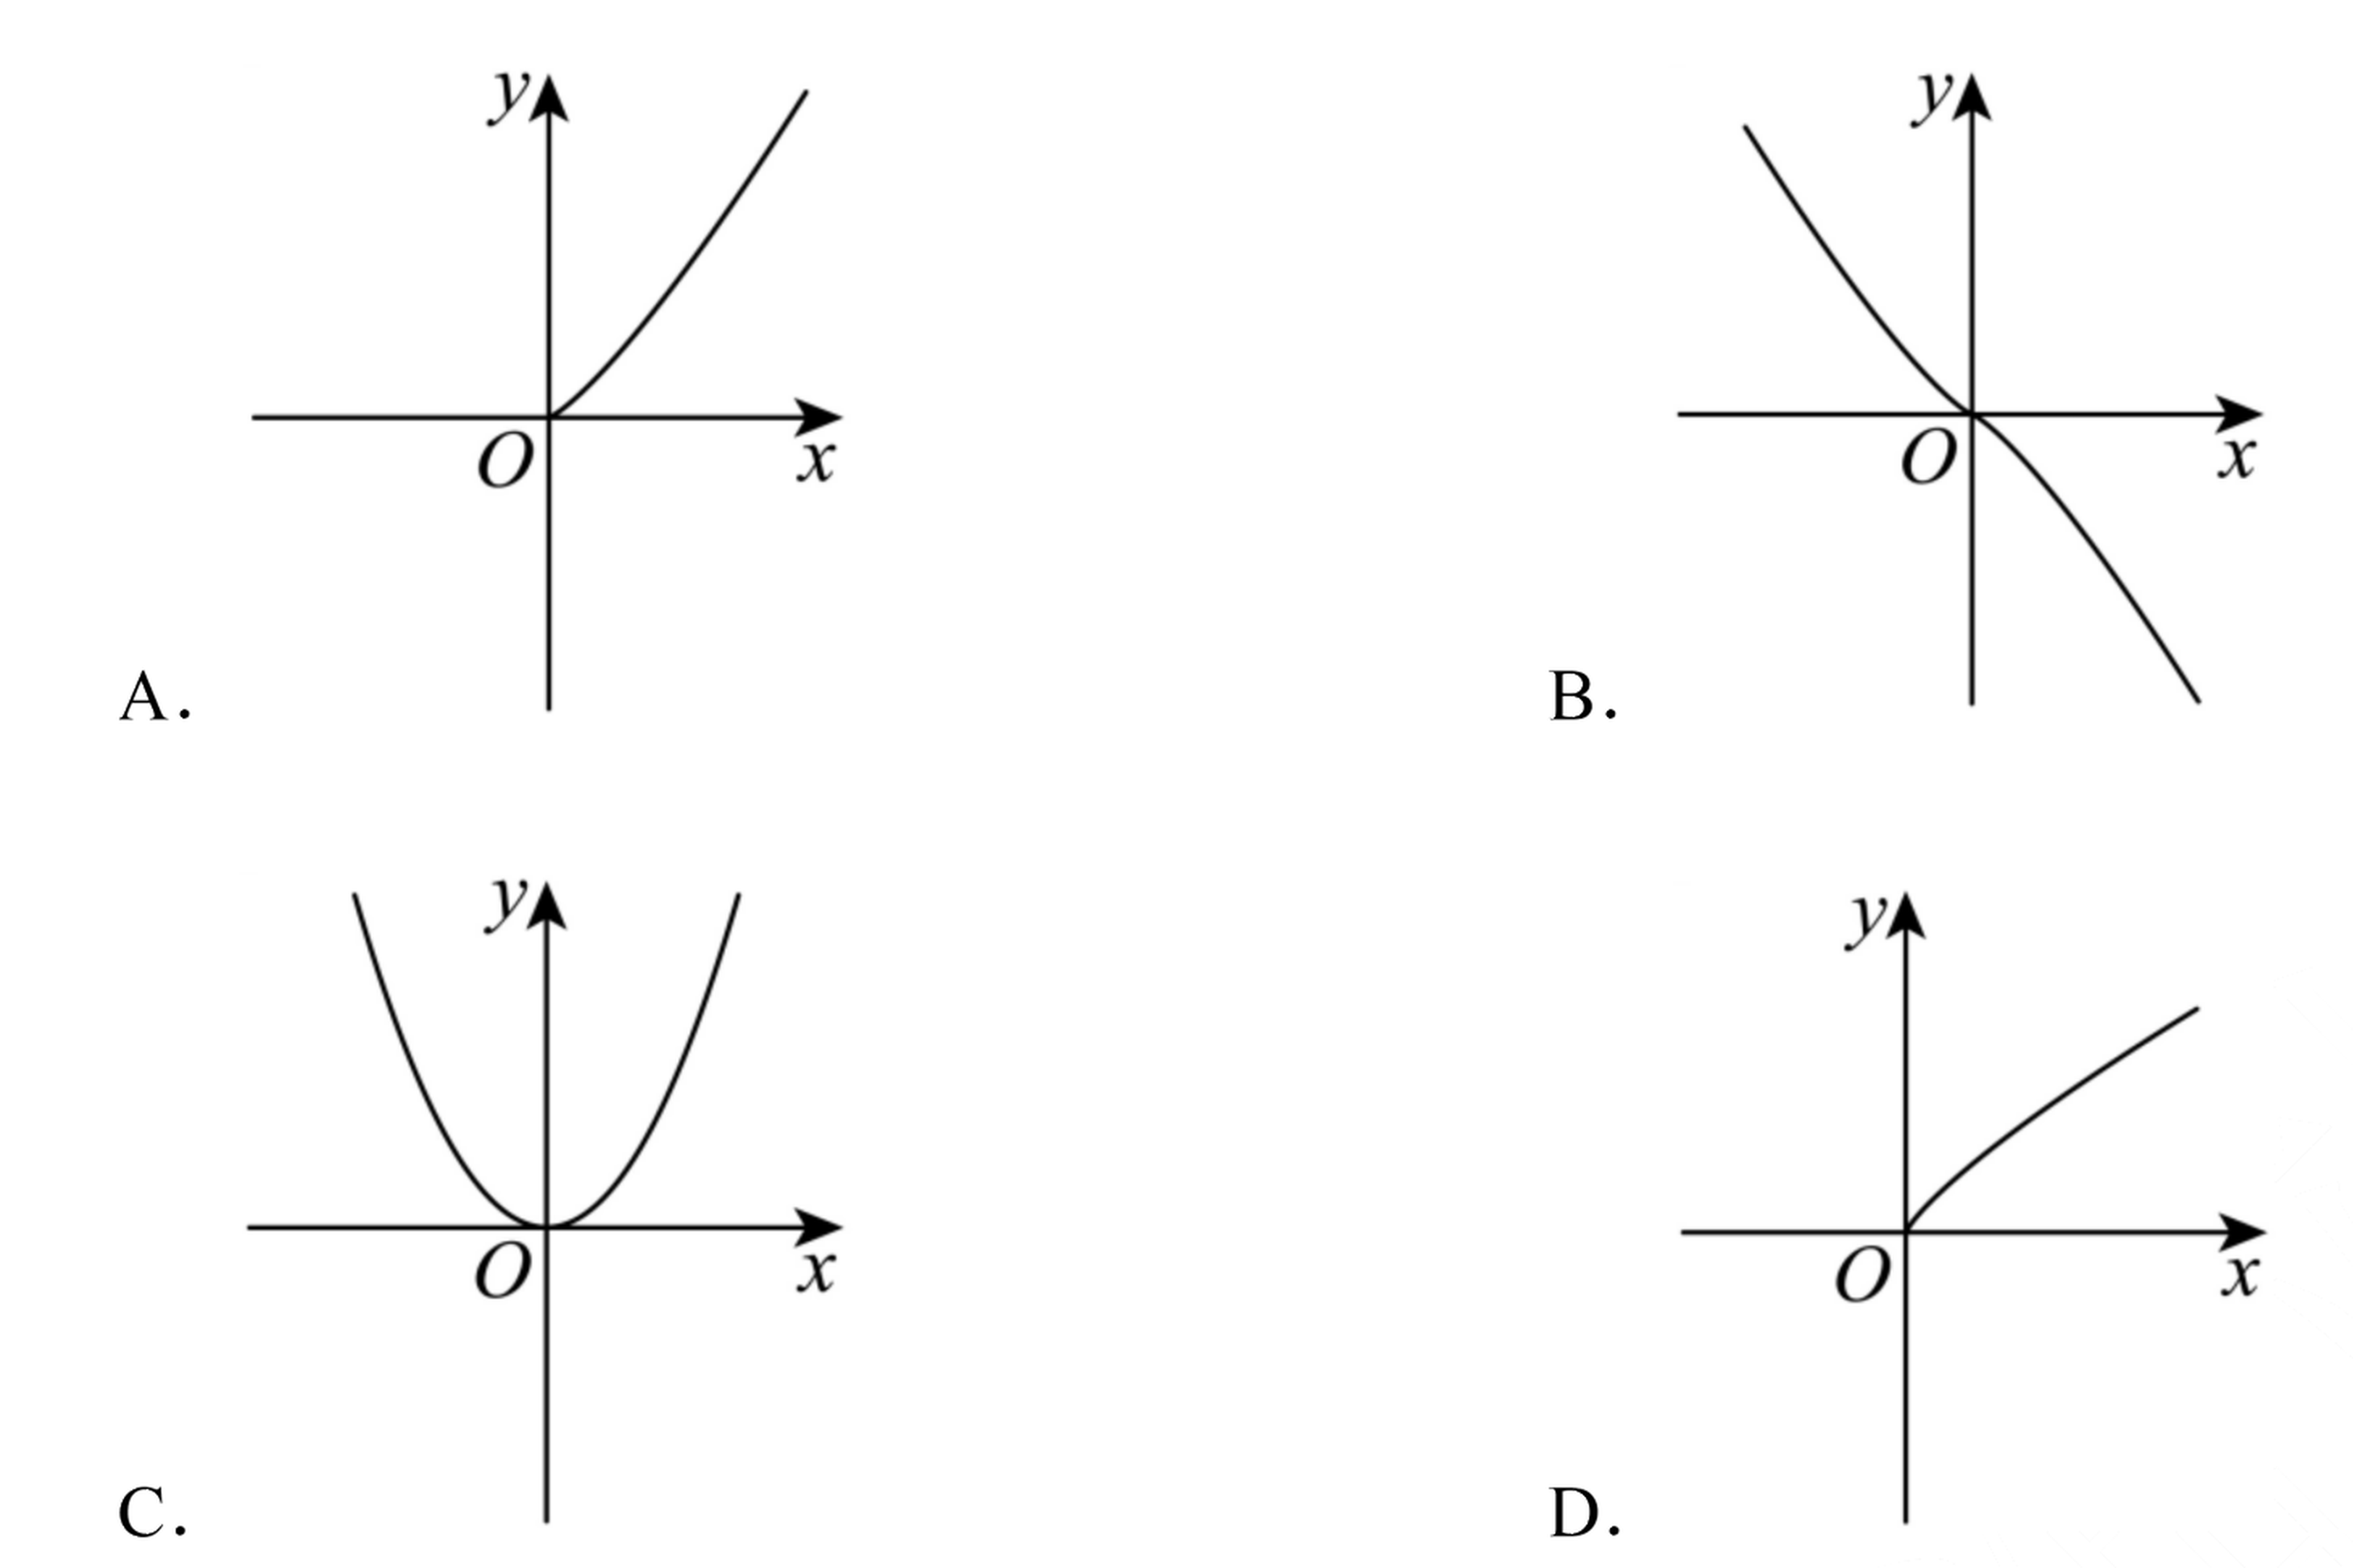
\includegraphics[width=0.80\textwidth]{figures/gao136_q13.png}
\end{center}

\ifanswer
\solbegin
\step{由 $y=x^{\frac54}=\sqrt[4]{x^5}$，函数的定义域为 $[0,+\infty)$，排除 BC，}% 原卷"排除 BC"连写，照录
\step{因为 $\dfrac54>1$，所以函数 $y=x^{\frac54}$ 的图象呈现下凸的趋势，排除 D. 故选 $A$.}
\solend
\fi

\item 下列不等式① $a+\dfrac1a\geqslant2$；② $a^2+4\geqslant4a$；③ $\left\lvert\dfrac ba+\dfrac ab\right\rvert\geqslant2$；④ $\dfrac{2a^2b^2}{a^2+b^2}\leqslant ab$；其中恒成立的是\mbox{（\quad）}

\keepwithprev
A. ①④\qquad B. ③④\qquad C. ②③\qquad D. ①②

\ifanswer
\ans{$C$}
\fi

\item 函数 $y=a^x+b-1(a>0,a\neq1)$ 单调递增且图象不经过第四象限，则 $a,b$ 满足的条件为\mbox{（\quad）}

\keepwithprev
A. $a>1,b\leqslant1$\qquad B. $a>1,b\geqslant0$\qquad C. $0<a<1,b\leqslant1$\qquad D. $0<a<1,b\geqslant1$

\ifanswer
\solbegin
\step{因为函数 $y=a^x+b-1$ 单调递增，所以 $a>1$，}
\step{图象不经过第四象限，则 $x=0$ 时，$y=b\geqslant0$，所以 $a>1,b\geqslant0$，故选 $B$.}
\solend
\fi

\item 设关于 $x$ 的不等式 $\dfrac{ax-1}{x^2-a}<0$ 的解集为 $S$，且 $3\in S$，$4\notin S$，则实数 $a$ 的取值范围为\mbox{（\quad）}

\keepwithprev
A. $(-\infty,-\sqrt3)\cup\left(\dfrac13,\sqrt3\right)$\qquad B. $\left(-\infty,\dfrac14\right)\cup(16,+\infty)$

C. $\left[\dfrac14,\dfrac13\right)\cup(9,16]$\qquad D. 不能确定

\ifanswer
\solbegin
\step{若 $3\in S$，则 $\dfrac{3a-1}{9-a}<0$，解得 $a\in\left(-\infty,\dfrac13\right)\cup(9,+\infty)$，}
\step{若 $4\notin S$，则 $16-a=0$ 或 $\dfrac{4a-1}{16-a}\geqslant0$，解得 $a\in\left[\dfrac14,16\right]$，}
\step{故实数 $a$ 的取值范围为 $\left[\dfrac14,\dfrac13\right)\cup(9,16]$，故选 $C$.}
\solend
\fi

\end{enumerate}

\bigsec{三、解答题}

\begin{enumerate}
\setcounter{enumi}{16}

\item 计算：(1) 计算 $\dfrac{\lg8+\lg125-\lg2-\lg5}{\lg\sqrt{10}\cdot\lg0.1}$；(2) 若 $a^{2x}=2(a>0)$，求 $\dfrac{a^{3x}+a^{-3x}}{a^x+a^{-x}}$.

\ifanswer
\solbegin
\step{(1) 原式 $=\dfrac{2-1}{\frac12\cdot(-1)}=-2$；(2) 原式 $=a^{2x}-1+a^{-2x}=2-1+\dfrac12=\dfrac32$.}
\solend
\fi

\item 不等式 $\dfrac{x-1}{x+1}\geqslant0$ 的解集为 $A$，不等式 $(x-a-1)(2a-x)>0(a<1)$ 的解集为 $B$.

(1) 求集合 $A$；

(2) 若 $B\subseteq A$，求实数 $a$ 的取值范围.

\ifanswer
\solbegin
\step{(1) $A=(-\infty,-1)\cup[1,+\infty)$.}
\step{(2) 由 $(x-a-1)(2a-x)>0(a<1)$，得 $(x-a-1)(x-2a)<0(a<1)$，}
\step{因为 $a<1$，所以 $a+1>2a$，所以 $B=(2a,a+1)$，}
\step{因为 $B\subseteq A$，所以 $2a\geqslant1$ 或 $a+1\leqslant-1$，即 $a\geqslant\dfrac12$ 或 $a\leqslant-2$，}
\step{而 $a<1$，所以实数 $a$ 的取值范围 $(-\infty,-2]\cup\left[\dfrac12,1\right)$.}% 原卷"取值范围"后脱"是／为"，照录
\solend
\fi

\item 已知幂函数 $y=x^m(m\in\R)$ 经过点 $\left(4,\dfrac12\right)$.

(1) 求此幂函数的表达式和定义域；

(2) 已知点 $A(a+2,y_1)$，点 $B(3-2a,y_2)(a\in\R)$ 在此幂函数的图像上，且满足 $y_1<y_2$，求实数 $a$ 的取值范围.

\ifanswer
\solbegin
\step{(1) 幂函数 $y=x^m(m\in\R)$ 经过点 $\left(4,\dfrac12\right)$，所以 $4^m=\dfrac12\Rightarrow m=-\dfrac12$，}
\step{所以 $f(x)=x^{-\frac12}$，定义域为 $(0,+\infty)$.}
\step{(2) 由于函数 $f(x)$ 在其定义域 $(0,+\infty)$ 上严格减，}
\step{由 $y_1<y_2$，得 $a+2>3-2a\geqslant0\Rightarrow a\in\left(\dfrac13,\dfrac32\right]$.}
\solend
\fi

% 第 20 题图取 05 页截图（0.42\textwidth、高约 6cm）。试排 \item 前加 7cm 守卫会多出
% 一张只有两行正文的稀疏页，且三版不加守卫时图均与题干、【解析】同页，故不另加守卫
\item 某医药研究所开发一种抗甲流新药，如果成年人按规定的剂量服用，据监测：服药后每毫升血液中的含药量 $y$（微克）与时间 $t$（小时）之间近似满足如图所示的曲线.

(1) 结合图，求 $k$ 与 $a$ 的值；

(2) 写出服药后 $y$ 与 $t$ 之间的函数关系式 $y=f(t)$；

(3) 据进一步测定：每毫升血液中含药量不少于 $0.5$ 微克时治疗疾病有效，求服药一次治疗有效的时间范围？

\begin{center}
% 图取原卷 05 页截图去粉色水印、去色，3x LANCZOS 放大
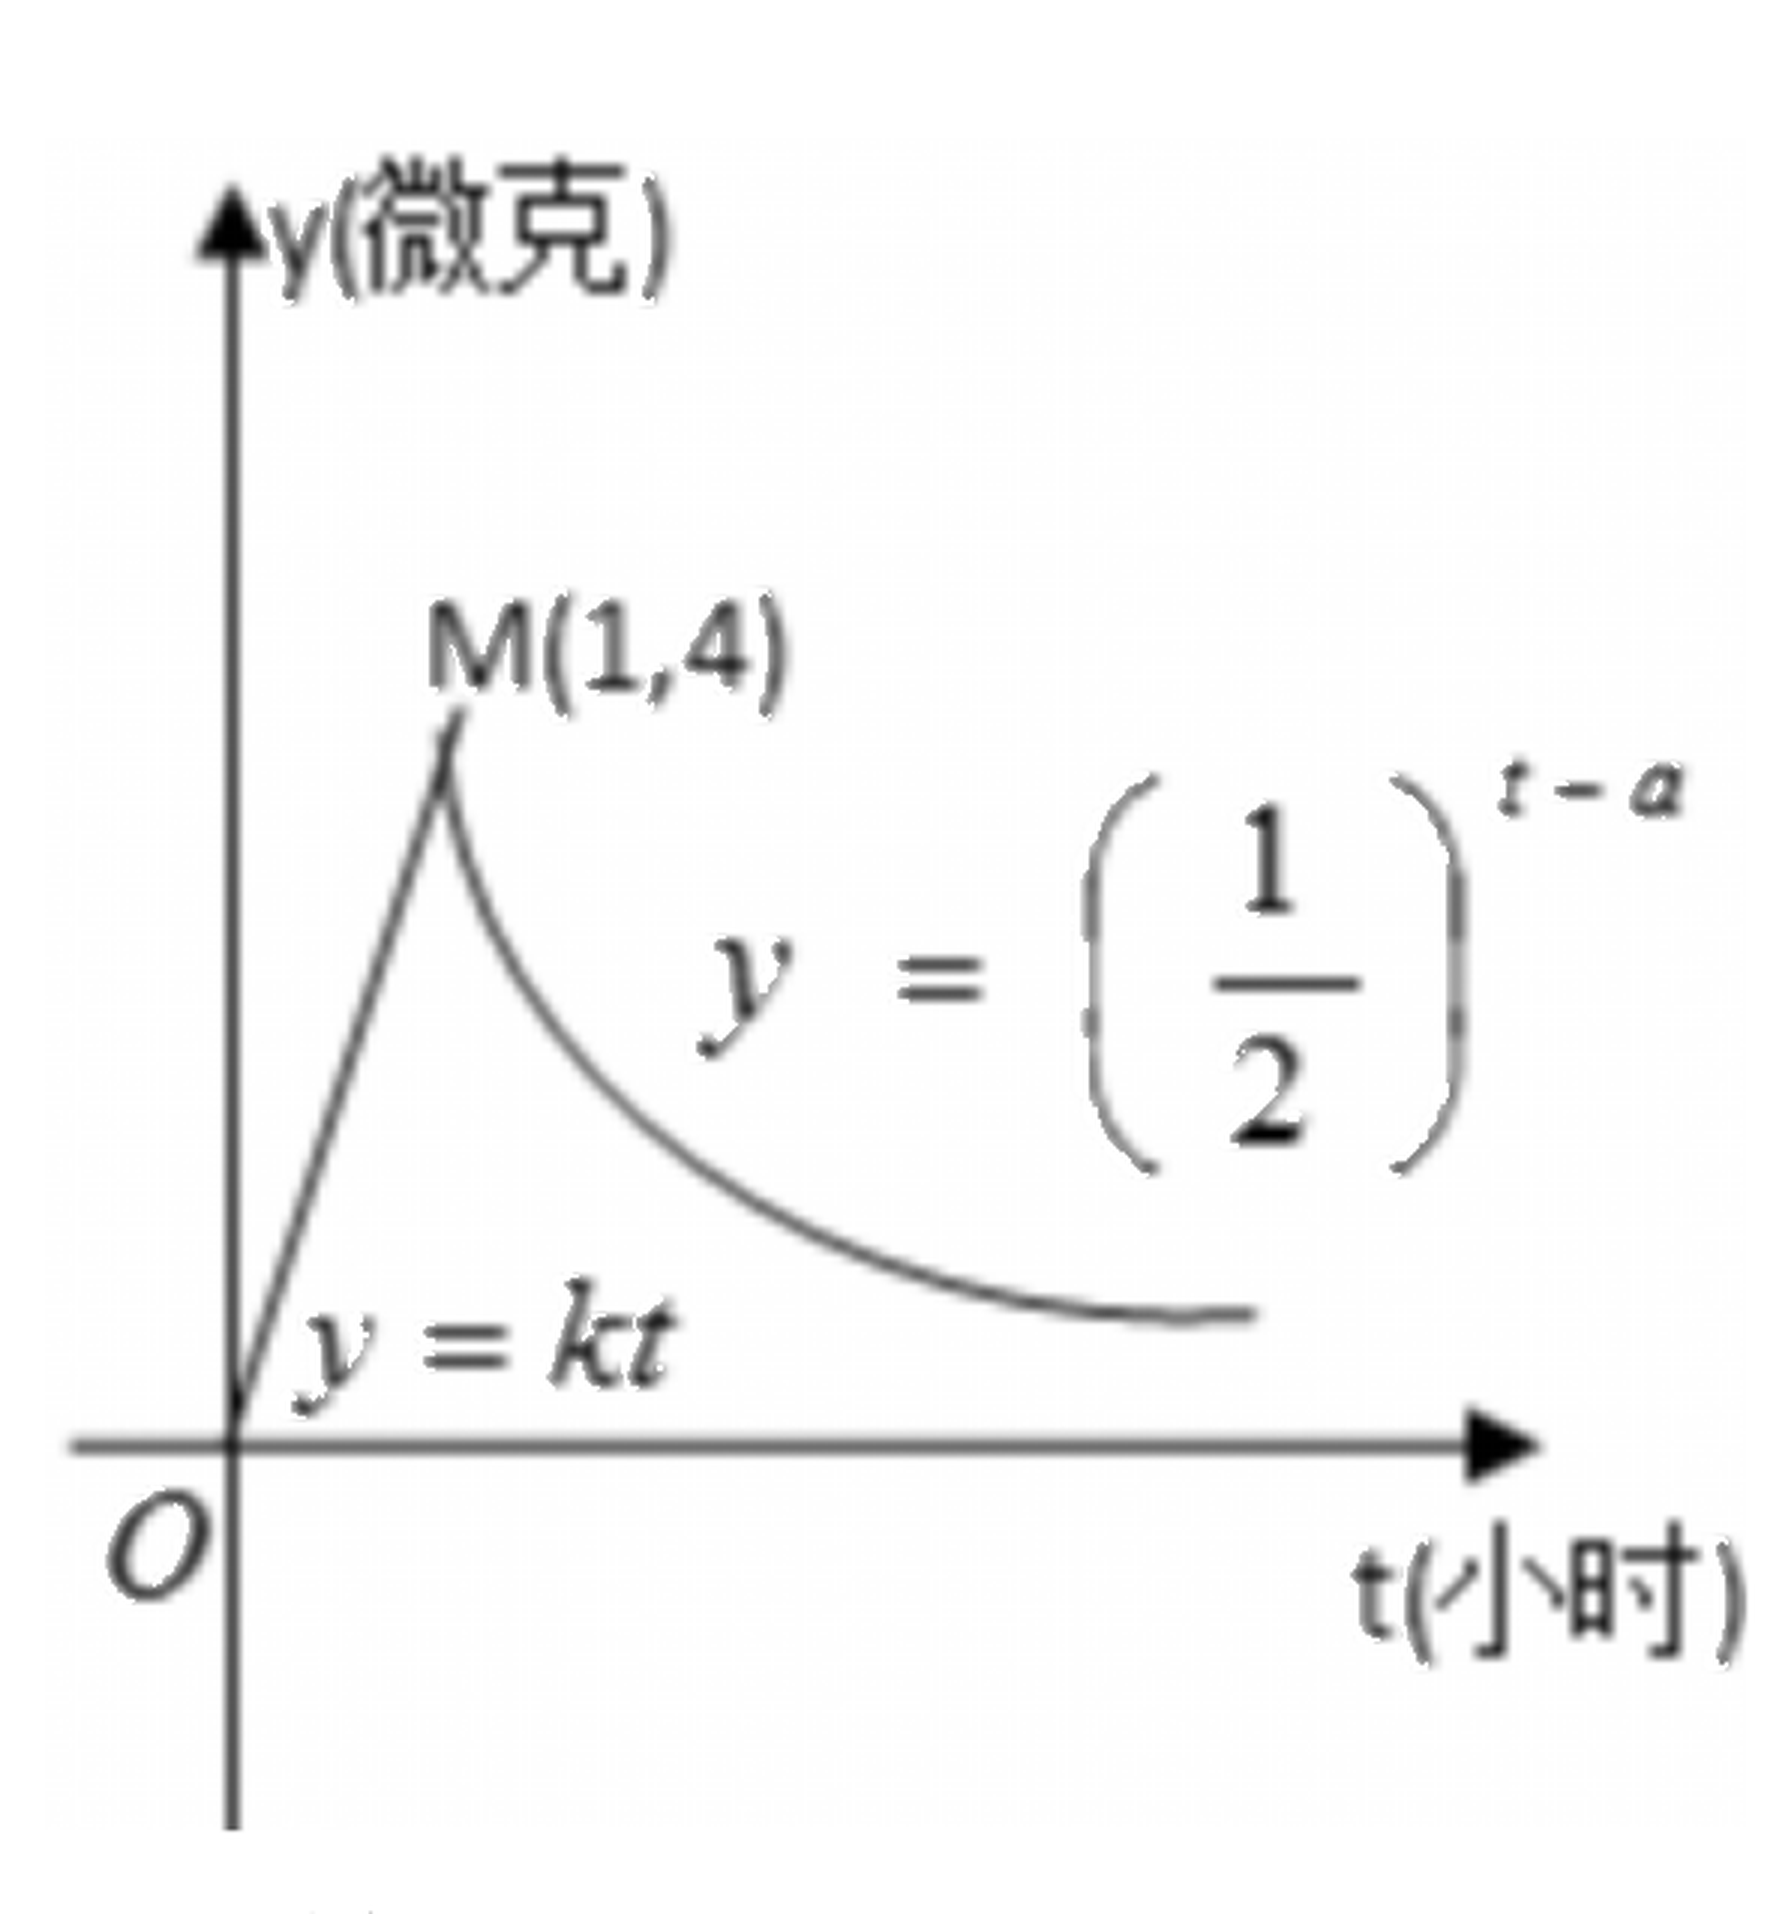
\includegraphics[width=0.42\textwidth]{figures/gao136_q20.png}
\end{center}

\ifanswer
\solbegin
\step{(1) 当 $0\leqslant t\leqslant1$ 时，函数图象是一条线段，由于过原点与点 $(1,4)$，所以 $k=4$，}
\step{其解析式为 $y=4t$，$0\leqslant t\leqslant1$；}
\step{当 $t\geqslant1$ 时，函数的解析式为 $y=\left(\dfrac12\right)^{t-a}$，}
\step{此时 $M(1,4)$ 在曲线上，将此点的坐标代入函数解析式得 $4=\left(\dfrac12\right)^{1-a}$，}
\step{解得 $a=3$；}
\step{(2) 由 (1) 得 $f(t)=\begin{cases}4t,0\leqslant t\leqslant1\\\left(\frac12\right)^{t-3},t>1\end{cases}$；}
\step{(3) 由 (2) 得，令 $f(t)\geqslant0.5$，即 $\begin{cases}4t\geqslant0.5,0\leqslant t\leqslant1\\\left(\frac12\right)^{t-3}\geqslant0.5,t>1\end{cases}$，所以 $\dfrac18\leqslant t\leqslant4$.}
\solend
\fi

\item 已知关于 $x$ 的不等式 $(kx-k^2-4)(x-4)>0$，其中 $k\in\R$.

(1) 当 $k=-1$，求不等式的解集 $A$；

(2) 当 $k$ 变化时，试求不等式的解集 $A$；

(3) 对于不等式解集 $A$，满足 $A\cap\Z=B$. 试探究集合 $B$ 能否为有限集，若能，求出使得集合 $B$ 中元素最少的 $k$ 的所有取值，并用列举法表示此时的集合 $B$，若不能，说明理由；

\ifanswer
\solbegin
\step{(1) 当 $k=-1$ 时，原不等式可化为 $(x+5)(x-4)<0$，}
\step{解得 $-5<x<4$，故不等式的解集为 $\{x\mid -5<x<4\}$；}
\step{(2) 当 $k=0$ 时，解集为 $\{x\mid x<4\}$，}
\step{当 $k>0$ 时，$\dfrac{k^2+4}{k}=k+\dfrac4k\geqslant4$，解集为 $\{x\mid x<4\text{ 或 }x>\dfrac{k^2+4}{k}\}$；}
\step{当 $k<0$ 时，解集为 $\{x\mid \dfrac{k^2+4}{k}<x<4\}$，}
\step{综上，当 $k=0$ 时，$A=\{x\mid x<4\}$，}
\step{当 $k>0$ 时，$A=\{x\mid x<4\text{ 或 }x>\dfrac{k^2+4}{k}\}$；}
\step{当 $k<0$ 时，$A=\{x\mid \dfrac{k^2+4}{k}<x<4\}$，}
\step{(3) 由 (2) 得当 $k\geqslant0$ 时，$B$ 为无限集，当 $k<0$ 时，$B$ 为有限集，}
\step{此时，$\dfrac{k^2+4}{k}=k+\dfrac4k\leqslant-4$，当且仅当 $k=-2$ 时取等号，}
\step{所以 $k=-2$ 时，$B$ 中元素最少，此时 $A=\{x\mid -4<x<4\}$，}
\step{所以 $B=\{-3,-2,-1,0,1,2,3\}$.}
\solend
\fi

\end{enumerate}

% 第 22 题是"四、附加题"首题且带 9cm 图块，守卫须放在 \bigsec 之前连节标题一起量，
% 否则"四、附加题"会孤立在页末（B 类，照 高一26／40／59 成例）
\needvspace{11cm}
\bigsec{四、附加题}

\begin{enumerate}
\setcounter{enumi}{21}

% 第 22 题四幅抛物线/坐标图选项是一整块，守卫放在 \item 之前
\needvspace{9cm}
\item 函数 $f(x)=\left(\dfrac12\right)^{\lvert x+1\rvert}$ 的图象大致为\mbox{（\quad）}

\keepwithprev
\begin{center}
% 四幅抛物线/坐标图选项取原卷 07 页截图去粉色水印，按原卷 2x2 排布合并为一张
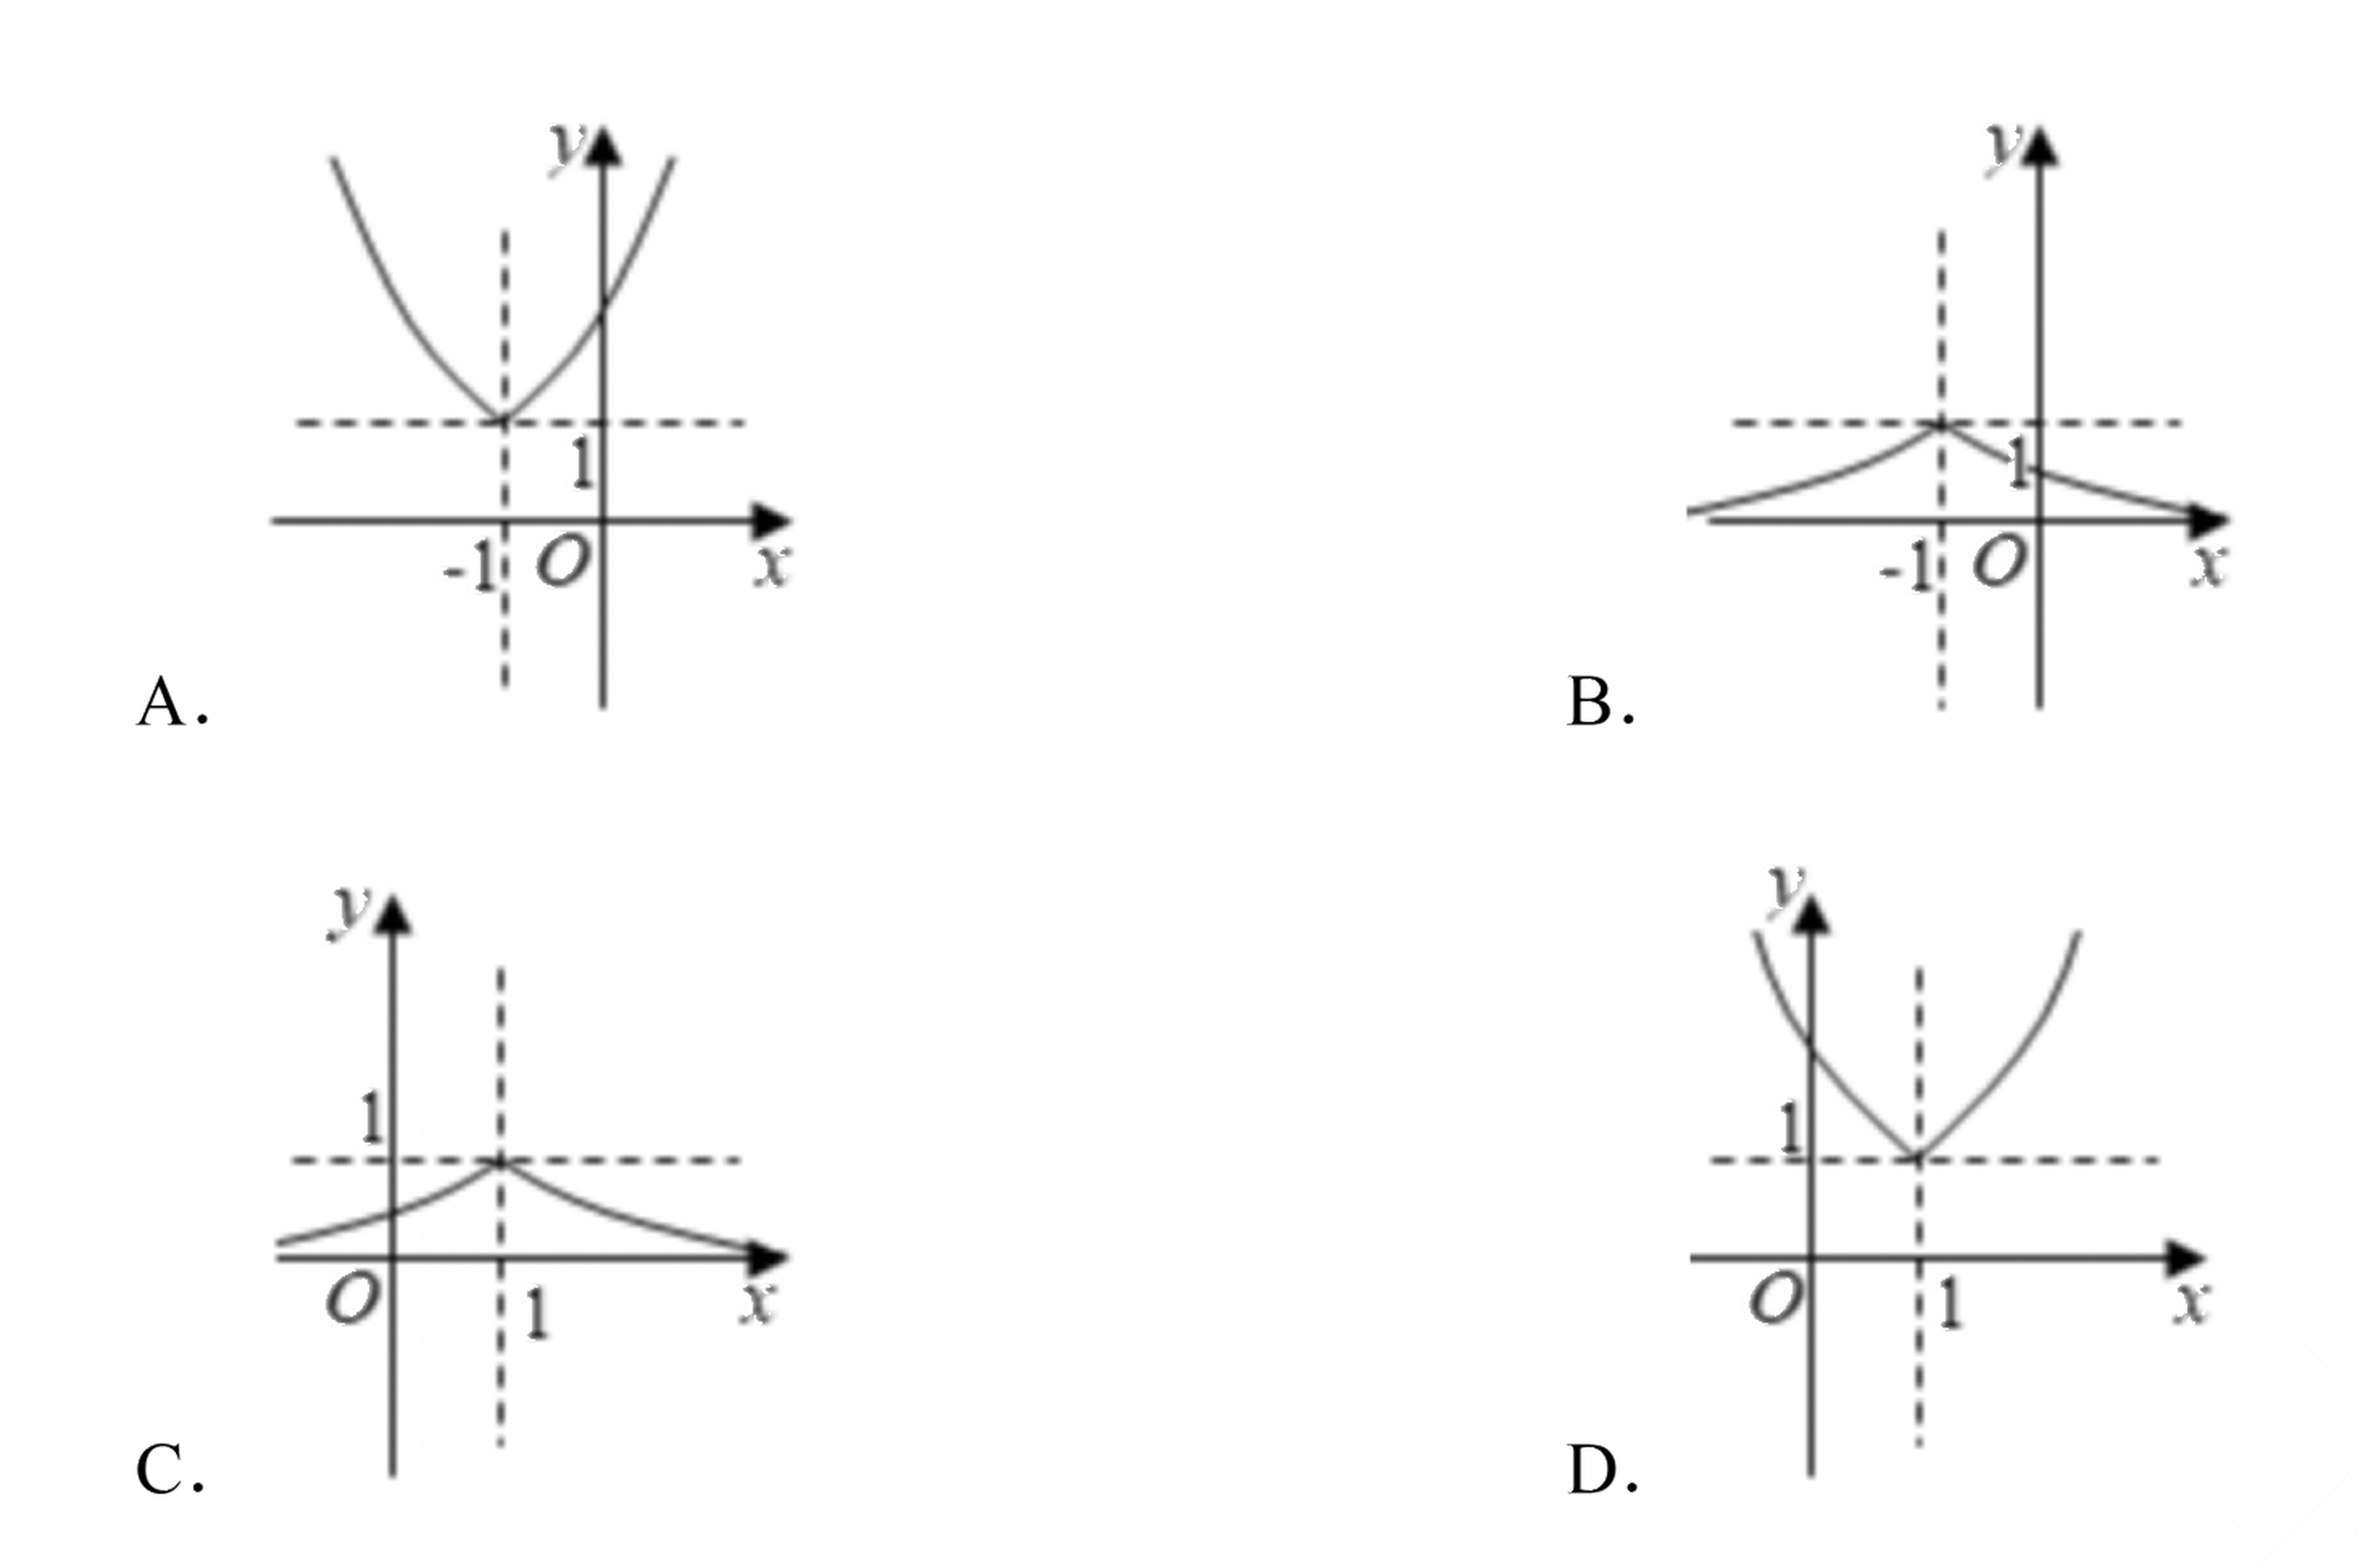
\includegraphics[width=0.80\textwidth]{figures/gao136_q22.png}
\end{center}

\ifanswer
\ans{$B$}
\fi

\end{enumerate}

\end{document}
"
%
% ① 原始材料：微信公众号"魔都数学加油站"文章，作者破晓，2026-11-15 18:04 发布；
% 连载"27学年高一136"，原文标题"27学年高一136——2026-2027年上海市三林中学高一上期中"；
% 原文链接：https://mp.weixin.qq.com/s/jaMzqMm6pDvcT0yM0d7eaQ。
% 正文为 7 张 PNG 页（01、04、06 为 4762x6735；02、03、05、07 为 2560x3620，
% 同一篇各页分辨率不同，逐页按各自分辨率裁图核对），题目下印有【答案】或【解析】，为讲评版。
% 题目、解析均据原图转录；卷面粉红色水印"魔都数学加油站"及公众号页脚未录入。
% 全卷 3 幅插图：第 13 题四幅坐标图选项（03 页）、第 20 题药物浓度折线/曲线图（05 页）、
% 第 22 题四幅抛物线/坐标图选项（07 页），均取原卷截图去粉色水印、去色、LANCZOS 放大，
% 四幅选项按原卷 2x2 排布合并为一张；图前按惯例加 \needvspace 守卫。
%
% 卷首标题：原卷印作"2026-2027 年三林中学高一上期中"（公众号标题中的"上海市"
% 卷面标题行没有，本稿照卷面），年份区间按全稿惯例排 en dash；原卷未印副标题，
% 本卷为期中卷、跨集合与常用逻辑用语／不等式／函数三章，按题目内容标为
% "集合与常用逻辑用语、不等式、函数"（与 125／126／128／129／131／132／133 同期中卷口径相同）：
% 集合与逻辑见 Q3、Q6、Q10、Q12、Q16、Q18、Q21，不等式见 Q5、Q7、Q8、Q9、Q14、Q15，
% 函数（幂函数、指数／对数、基本不等式应用）见 Q4、Q11、Q13、Q17、Q19、Q20、Q22。
%
% 题号体例：本卷共 20 题——一、填空题 3—12（10 题）、二、选择题 13—16（4 题）、
% 三、解答题 17—21（5 题）、四、附加题 22（1 题）。四节分别
% \setcounter{enumi}{2}／{12}／{16}／{21}。
%
% ② 与原卷的排版差异：
%   ① 原文从第 3 题起，本稿保留原题号；末节"四、附加题"另起 \bigsec，题号续到 22；
%   ② 原卷每题下直接印【答案】或【解析】，本稿按全稿惯例置于答案版；第 3、4、6 题只印
%      【答案】、无【解析】，提 \ans{}；第 14 题答案 C 印在题干括号内、无【解析】，按
%      高一53／高一108／高一132／高一133 成例括号留空、另提 \ans{$C$}；第 22 题答案 B
%      印在题干括号内、无【解析】，同例提 \ans{$B$}；第 13、15、16 题答案在解析末句
%      "故选 …"，括号内留空、不另提 \ans{}；其余各题印【解析】、无独立答案段；
%   ③ 原卷未印副标题，本稿按"知识模块"口径补出；
%   ④ 原卷填空横线按全稿惯例排为 \blankline[4.4em]；选择题括号排 \mbox{（\quad）}、
%      每个选项段前按惯例加 \keepwithprev（四幅图选项那一枚放在 \begin{center} 之前）；
%      解答题不留作答区、不加 \anspace（原卷为讲评版，与 129／131／132／133 同）；
%   ⑤ 原卷数集排斜体 $R$／$R^+$／$Z$，按全稿惯例改 \R／\R^+／\Z；空集记号 \varnothing；
%      绝对值排 \lvert…\rvert，集合描述竖线排 \mid；不等号按全稿惯例排 \leqslant／\geqslant；
%   ⑥ 子题标号 (1)(2)(3) 原卷用半角括号，照录；圈数字 ①②③④ 照录；第 12 题甲／乙／丙
%      三行与第 14 题四个编号不等式照录；
%   ⑦ 数学式内半角逗号照录（如 Q4"$a>0,a\neq1$"、Q6"$\{(-2,4),(1,1)\}$"、
%      Q7"$a=2+3=5,b=2\times3=6$"、Q11"$x_1,x_2$"、Q12"$m,n\in R^+$"、
%      Q15"$a>1,b\geq0$"、Q18"$B=(2a,a+1)$"、Q20"$4t,0\leq t\leq1$"、
%      Q21"$\{-3,-2,-1,0,1,2,3\}$"）；原卷行末西文句点照录，行中全角逗号照录；
%   ⑧ 三幅插图：第 13 题四幅坐标图选项合并裁为一张 \includegraphics（题前 \needvspace{9cm}）；
%      第 20 题折线/曲线图取 05 页截图（0.42\textwidth）；第 22 题四幅抛物线/坐标图选项合并
%      裁为一张（题前 \needvspace{9cm}）。第 13、22 题分别是"二、选择题""四、附加题"的首题
%      且带大图块，另在两处 \bigsec 之前各加 \needvspace{11cm} 连节标题一起量，避免节标题
%      孤立在页末（切页审计 B 类；照 高一26／40／59 成例）。第 20 题图不是节首题、三版试排
%      图均与题干同页，加 7cm 守卫反会多出一张只有两行正文的稀疏页，故不另加守卫；
%      三版切页审计均"合计异常：无"（试卷 4 页／紧凑 4 页／答案 6 页）；
%   ⑨ 跨页续印按题合并：Q16 题干在 03 页、括号与选项及【解析】在 04 页；Q19 题干在 04 页、
%      (2) 与【解析】在 05 页；Q20 (3)【解析】在 06 页；Q22 四幅图在 07 页；本稿按题连排；
%   ⑩ 题干中的中文弯引号按原卷照录，注释内一律 ASCII 引号；原卷"图像／图象"两种写法混用，
%      逐处照录（Q4、Q19 作"图像"，Q13、Q15、Q20、Q22 作"图象"）；
%   ⑪ 附加题节：原卷印"四、附加题"，本稿用 \bigsec{四、附加题} 另起一节、
%      \setcounter{enumi}{21}，顶层 1 个 \item（与 高一09／15／16／22／35／39／47／61 同口径）；
%      Q22 只印括号内答案、提 \ans{}，不计入 \step 账。
%
% 判别式字形：全卷仅第 9 题【解析】cases 块出现判别式"$\Delta=a^2-8a<0$"，原卷印
%   等腰、偏高的三角 $\Delta$，逐处放大核对并照录 \Delta；全卷未出现扁等边三角 \triangle。
%
% 子集符号：第 18 题 (2) 题干"$B\subseteq A$"与【解析】"$B\subseteq A$"两处原卷均印
%   带下划线 $\subseteq$，逐处放大核对、照录 \subseteq；全卷未出现单线 \subset。
%
% 原卷存疑照录（均照录未改，正文对应处另有 % 注）：
%   第 12 题乙行"$\dfrac{m+n}{mm}=\dfrac1{mn}$"前一分母印作 $mm$（后一处作 $mn$），照录；
%   第 12 题【解析】"$\geqslant\dfrac1{100}\left[a^2+1+2\sqrt{a^2}\right]$"保留 $\sqrt{a^2}$
%      未化简为 $a$，照录；
%   第 13 题【解析】"排除 BC"与"排除 D"连写选项字母，照录；
%   第 18 题 (2)【解析】末行"所以实数 $a$ 的取值范围 $(-\infty,-2]\cup[\frac12,1)$"
%      "取值范围"后脱"是／为"字，照录；
%   第 21 题 (3) 题干"求出使得集合 $B$ 中元素最少的 $k$ 的所有取值"而【解析】只给出
%      $k=-2$ 一处，措辞照录。
%
% 行数复核：逐题数 \step 条数，合计 51 条（Q3：0；Q4：0；Q5：2；Q6：0；Q7：2；Q8：1；
% Q9：1；Q10：4；Q11：1；Q12：4；Q13：2；Q14：0；Q15：2；Q16：3；Q17：1；Q18：5；
% Q19：4；Q20：7；Q21：12；Q22：0），与原卷印刷行逐题相等（cases 块作一个印刷行计）。
% 第 3、4、6、14、22 题只印【答案】、提 \ans{}，不计入 \step 账；第 13、15、16 题答案在
% 解析末句，括号内留空、不另提 \ans{}。
%
\documentclass[a4paper,11pt]{article}
\usepackage{common}

\begin{document}

\examtitlest[3]{2026--2027 年三林中学高一上期中}{集合与常用逻辑用语、不等式、函数}

\bigsec{一、填空题}

\begin{enumerate}
\setcounter{enumi}{2}

\item 用反证法证明命题“若 $x+y\neq5$，则 $x\neq2$ 或 $y\neq3$”为真命题时，第一个步骤是\blankline[4.4em].

\ifanswer
\ans{假设 $x=2$ 且 $y=3$}
\fi

\item 函数 $y=a^{x-1}+1(a>0,a\neq1)$ 的图像恒过定点 $A$，则点的坐标是\blankline[4.4em].

\ifanswer
\ans{$(1,2)$}
\fi

\item 已知 $x>1$，则 $x+\dfrac4{x-1}$ 的最小值是\blankline[4.4em].

\ifanswer
\solbegin
\step{由 $x>1$，得 $x-1>0$，则 $x+\dfrac4{x-1}=x-1+\dfrac4{x-1}+1\geqslant2\sqrt{(x-1)\cdot\dfrac4{x-1}}+1=5$，}
\step{当且仅当 $x-1=\dfrac4{x-1}$ 即 $x=3$ 时取等号，取得最小值 $5$.}
\solend
\fi

\item 已知集合 $A=\{(x,y)\mid y=x^2\}$，集合 $B=\{(x,y)\mid y=2-x\}$，求 $A\cap B=$\blankline[4.4em].

\ifanswer
\ans{$\{(-2,4),(1,1)\}$}
\fi

\item 已知一元二次不等式 $x^2-ax+b<0$ 的解集为 $(2,3)$，则不等式 $bx^2-ax+1>0$ 的解集是\blankline[4.4em].

\ifanswer
\solbegin
\step{$a=2+3=5,b=2\times3=6$，则 $bx^2-ax+1>0$ 即 $6x^2-5x+1>0$，}
\step{即 $(3x-1)(2x-1)>0$，解集为 $\left(-\infty,\dfrac13\right)\cup\left(\dfrac12,+\infty\right)$.}
\solend
\fi

\item 不等式 $(x+2)^3<(5-2x)^3$ 的解集为\blankline[4.4em].

\ifanswer
\solbegin
\step{由 $(x+2)^3<(5-2x)^3$ 得 $x+2<5-2x$，故解集为 $(-\infty,1)$.}
\solend
\fi

\item 若关于 $x$ 的不等式 $ax^2-ax+2>0$ 的解集为 $\R$，则实数 $a$ 的取值范围是\blankline[4.4em].

\ifanswer
\solbegin
\step{由题意得 $a=0$ 或 $\begin{cases}a>0\\\Delta=a^2-8a<0\end{cases}$，所以 $0\leqslant a<8$.}% 判别式原卷印高三角 $\Delta$，照录
\solend
\fi

\item 已知关于 $x$ 的不等式 $\lvert x+3\rvert+\lvert x-a\rvert\geqslant5$ 恒成立，则实数 $a$ 的取值范围为\blankline[4.4em].

\ifanswer
\solbegin
\step{因为 $\lvert x+3\rvert+\lvert x-a\rvert\geqslant\lvert x-a-x-3\rvert=\lvert 3+a\rvert$，}
\step{要使 $\lvert x+3\rvert+\lvert x-a\rvert\geqslant5$ 恒成立，则 $\lvert a+3\rvert\geqslant5$ 即可，}
\step{所以 $a+3\geqslant5$ 或 $a+3\leqslant-5$，解得 $a\geqslant2$ 或 $a\leqslant-8$，}
\step{即实数 $a$ 的取值范围是 $(-\infty,-8]\cup[2,+\infty)$.}
\solend
\fi

\item 若方程 $\lg^2 x-2\lg x-2=0$ 的两个解为 $x_1,x_2$，求 $\log_{x_1}x_2+\log_{x_2}x_1$ 的值为\blankline[4.4em].

\ifanswer
\solbegin
\step{$\log_{x_1}x_2+\log_{x_2}x_1=\dfrac{\lg x_2}{\lg x_1}+\dfrac{\lg x_1}{\lg x_2}=\dfrac{(\lg x_1+\lg x_2)^2-2\lg x_1\lg x_2}{\lg x_1\lg x_2}=-4$.}
\solend
\fi

\item 三个同学对问题“已知 $m,n\in \R^+$，且 $m+n=1$，求 $\dfrac1m+\dfrac1n$ 的最小值”提出各自的解题思路：

思路：

甲：$\dfrac1m+\dfrac1n=\dfrac{m+n}{m}+\dfrac{m+n}{n}=2+\dfrac nm+\dfrac mn$，可用基本不等式求解；

乙：$\dfrac1m+\dfrac1n=\dfrac{m+n}{mm}=\dfrac1{mn}=\dfrac1{m(1-m)}$，可用二次函数配方法求解；% 原卷前一分母印作 $mm$，照录

丙：$\dfrac1m+\dfrac1n=\left(\dfrac1m+\dfrac1n\right)(m+n)=2+\dfrac nm+\dfrac mn$，可用基本不等式求解；参考上述解题思路，

可求得当 $x=$\blankline[4.4em]时，$y=\dfrac{a^2}{x^2}+\dfrac1{100-x^2}$（$0<x<10$，$a>0$）有最小值.

\ifanswer
\solbegin
\step{$y=\dfrac{a^2}{x^2}+\dfrac1{100-x^2}=\left(\dfrac{a^2}{x^2}+\dfrac1{100-x^2}\right)[x^2+(100-x^2)]\times\dfrac1{100}$}
\step{$=\dfrac1{100}\left[a^2+1+\dfrac{x^2}{100-x^2}+\dfrac{a^2(100-x^2)}{x^2}\right]\geqslant\dfrac1{100}\left[a^2+1+2\sqrt{a^2}\right]$}% 原卷保留 $\sqrt{a^2}$ 未化简，照录
\step{当且仅当 $\dfrac{x^2}{100-x^2}=\dfrac{a^2(100-x^2)}{x^2}$，即 $x=\sqrt{\dfrac{100a}{a+1}}$ 时，}
\step{$y=\dfrac{a^2}{x^2}+\dfrac1{100-x^2}(0<x<10,a>0)$ 有最小值.}
\solend
\fi

\end{enumerate}

% 第 13 题是"二、选择题"首题且带 9cm 图块，守卫须放在 \bigsec 之前连节标题一起量，
% 否则"二、选择题"会孤立在页末（B 类，照 高一26／40／59 成例）
\needvspace{11cm}
\bigsec{二、选择题}

\begin{enumerate}
\setcounter{enumi}{12}

% 第 13 题四幅坐标图选项是一整块，守卫放在 \item 之前
\needvspace{9cm}
\item 下列图象中，最符合函数 $y=x^{\frac54}$ 的图象的是\mbox{（\quad）}

\keepwithprev
\begin{center}
% 四幅坐标图选项取原卷 03 页截图去粉色水印，按原卷 2x2 排布合并为一张
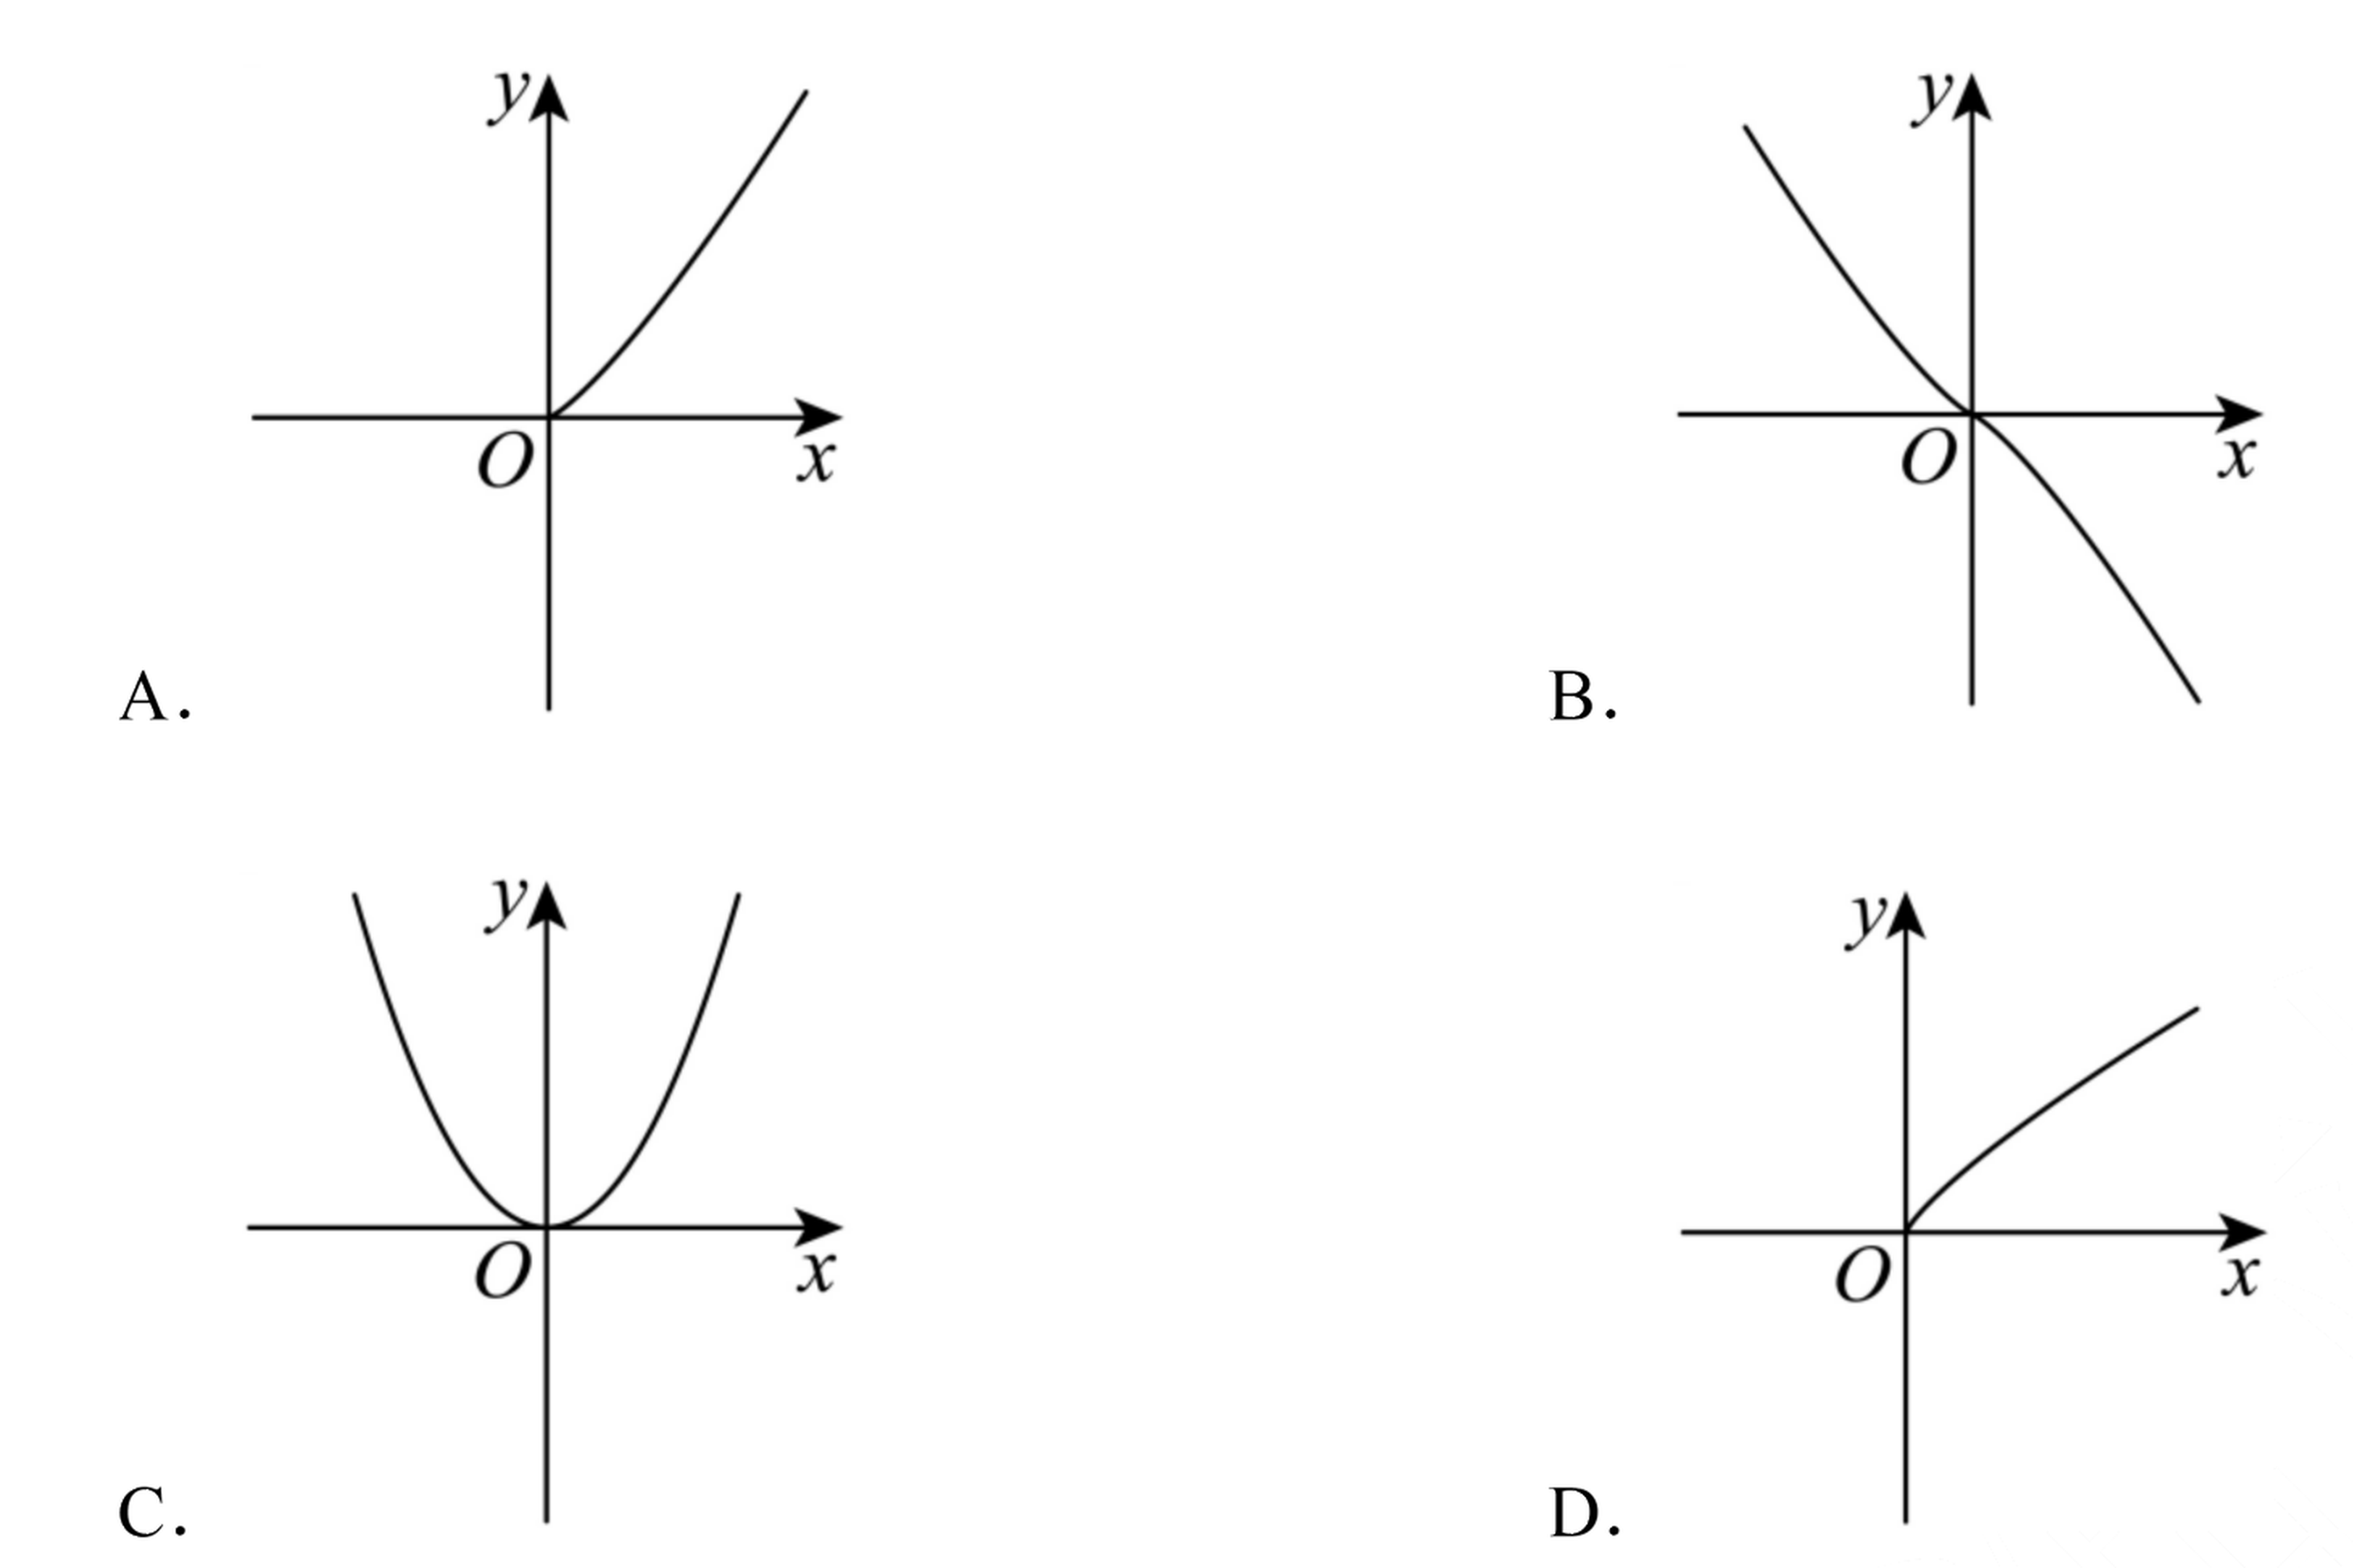
\includegraphics[width=0.80\textwidth]{figures/gao136_q13.png}
\end{center}

\ifanswer
\solbegin
\step{由 $y=x^{\frac54}=\sqrt[4]{x^5}$，函数的定义域为 $[0,+\infty)$，排除 BC，}% 原卷"排除 BC"连写，照录
\step{因为 $\dfrac54>1$，所以函数 $y=x^{\frac54}$ 的图象呈现下凸的趋势，排除 D. 故选 $A$.}
\solend
\fi

\item 下列不等式① $a+\dfrac1a\geqslant2$；② $a^2+4\geqslant4a$；③ $\left\lvert\dfrac ba+\dfrac ab\right\rvert\geqslant2$；④ $\dfrac{2a^2b^2}{a^2+b^2}\leqslant ab$；其中恒成立的是\mbox{（\quad）}

\keepwithprev
A. ①④\qquad B. ③④\qquad C. ②③\qquad D. ①②

\ifanswer
\ans{$C$}
\fi

\item 函数 $y=a^x+b-1(a>0,a\neq1)$ 单调递增且图象不经过第四象限，则 $a,b$ 满足的条件为\mbox{（\quad）}

\keepwithprev
A. $a>1,b\leqslant1$\qquad B. $a>1,b\geqslant0$\qquad C. $0<a<1,b\leqslant1$\qquad D. $0<a<1,b\geqslant1$

\ifanswer
\solbegin
\step{因为函数 $y=a^x+b-1$ 单调递增，所以 $a>1$，}
\step{图象不经过第四象限，则 $x=0$ 时，$y=b\geqslant0$，所以 $a>1,b\geqslant0$，故选 $B$.}
\solend
\fi

\item 设关于 $x$ 的不等式 $\dfrac{ax-1}{x^2-a}<0$ 的解集为 $S$，且 $3\in S$，$4\notin S$，则实数 $a$ 的取值范围为\mbox{（\quad）}

\keepwithprev
A. $(-\infty,-\sqrt3)\cup\left(\dfrac13,\sqrt3\right)$\qquad B. $\left(-\infty,\dfrac14\right)\cup(16,+\infty)$

C. $\left[\dfrac14,\dfrac13\right)\cup(9,16]$\qquad D. 不能确定

\ifanswer
\solbegin
\step{若 $3\in S$，则 $\dfrac{3a-1}{9-a}<0$，解得 $a\in\left(-\infty,\dfrac13\right)\cup(9,+\infty)$，}
\step{若 $4\notin S$，则 $16-a=0$ 或 $\dfrac{4a-1}{16-a}\geqslant0$，解得 $a\in\left[\dfrac14,16\right]$，}
\step{故实数 $a$ 的取值范围为 $\left[\dfrac14,\dfrac13\right)\cup(9,16]$，故选 $C$.}
\solend
\fi

\end{enumerate}

\bigsec{三、解答题}

\begin{enumerate}
\setcounter{enumi}{16}

\item 计算：(1) 计算 $\dfrac{\lg8+\lg125-\lg2-\lg5}{\lg\sqrt{10}\cdot\lg0.1}$；(2) 若 $a^{2x}=2(a>0)$，求 $\dfrac{a^{3x}+a^{-3x}}{a^x+a^{-x}}$.

\ifanswer
\solbegin
\step{(1) 原式 $=\dfrac{2-1}{\frac12\cdot(-1)}=-2$；(2) 原式 $=a^{2x}-1+a^{-2x}=2-1+\dfrac12=\dfrac32$.}
\solend
\fi

\item 不等式 $\dfrac{x-1}{x+1}\geqslant0$ 的解集为 $A$，不等式 $(x-a-1)(2a-x)>0(a<1)$ 的解集为 $B$.

(1) 求集合 $A$；

(2) 若 $B\subseteq A$，求实数 $a$ 的取值范围.

\ifanswer
\solbegin
\step{(1) $A=(-\infty,-1)\cup[1,+\infty)$.}
\step{(2) 由 $(x-a-1)(2a-x)>0(a<1)$，得 $(x-a-1)(x-2a)<0(a<1)$，}
\step{因为 $a<1$，所以 $a+1>2a$，所以 $B=(2a,a+1)$，}
\step{因为 $B\subseteq A$，所以 $2a\geqslant1$ 或 $a+1\leqslant-1$，即 $a\geqslant\dfrac12$ 或 $a\leqslant-2$，}
\step{而 $a<1$，所以实数 $a$ 的取值范围 $(-\infty,-2]\cup\left[\dfrac12,1\right)$.}% 原卷"取值范围"后脱"是／为"，照录
\solend
\fi

\item 已知幂函数 $y=x^m(m\in\R)$ 经过点 $\left(4,\dfrac12\right)$.

(1) 求此幂函数的表达式和定义域；

(2) 已知点 $A(a+2,y_1)$，点 $B(3-2a,y_2)(a\in\R)$ 在此幂函数的图像上，且满足 $y_1<y_2$，求实数 $a$ 的取值范围.

\ifanswer
\solbegin
\step{(1) 幂函数 $y=x^m(m\in\R)$ 经过点 $\left(4,\dfrac12\right)$，所以 $4^m=\dfrac12\Rightarrow m=-\dfrac12$，}
\step{所以 $f(x)=x^{-\frac12}$，定义域为 $(0,+\infty)$.}
\step{(2) 由于函数 $f(x)$ 在其定义域 $(0,+\infty)$ 上严格减，}
\step{由 $y_1<y_2$，得 $a+2>3-2a\geqslant0\Rightarrow a\in\left(\dfrac13,\dfrac32\right]$.}
\solend
\fi

% 第 20 题图取 05 页截图（0.42\textwidth、高约 6cm）。试排 \item 前加 7cm 守卫会多出
% 一张只有两行正文的稀疏页，且三版不加守卫时图均与题干、【解析】同页，故不另加守卫
\item 某医药研究所开发一种抗甲流新药，如果成年人按规定的剂量服用，据监测：服药后每毫升血液中的含药量 $y$（微克）与时间 $t$（小时）之间近似满足如图所示的曲线.

(1) 结合图，求 $k$ 与 $a$ 的值；

(2) 写出服药后 $y$ 与 $t$ 之间的函数关系式 $y=f(t)$；

(3) 据进一步测定：每毫升血液中含药量不少于 $0.5$ 微克时治疗疾病有效，求服药一次治疗有效的时间范围？

\begin{center}
% 图取原卷 05 页截图去粉色水印、去色，3x LANCZOS 放大
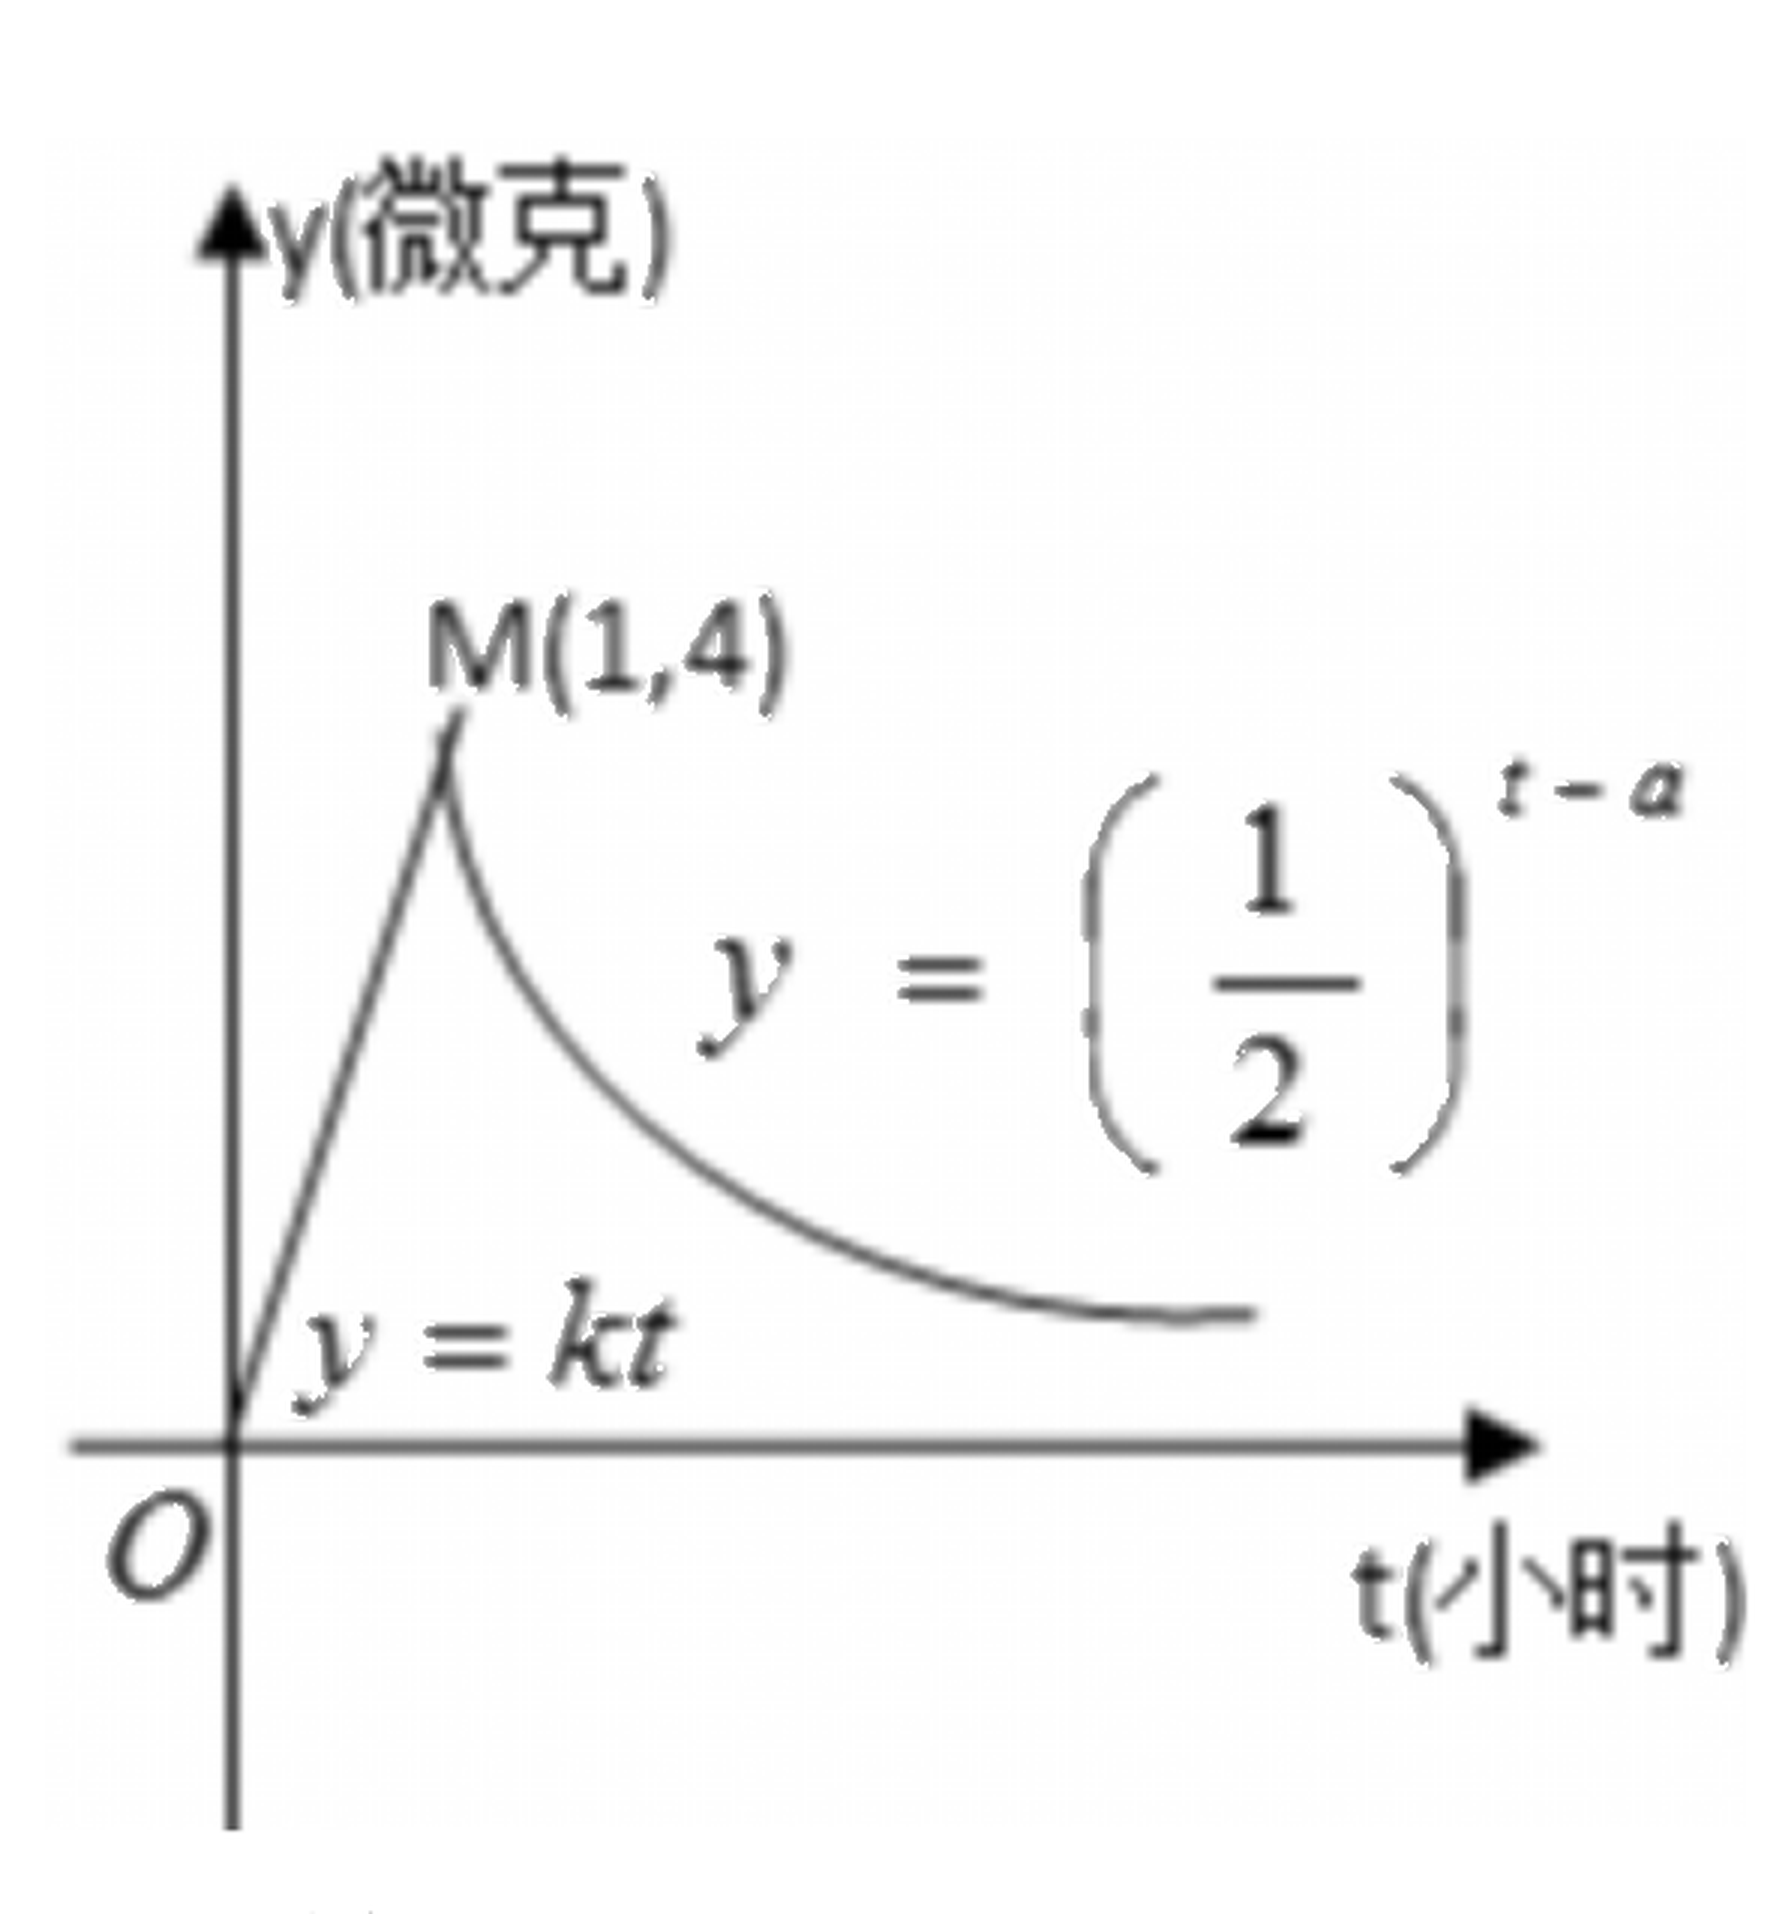
\includegraphics[width=0.42\textwidth]{figures/gao136_q20.png}
\end{center}

\ifanswer
\solbegin
\step{(1) 当 $0\leqslant t\leqslant1$ 时，函数图象是一条线段，由于过原点与点 $(1,4)$，所以 $k=4$，}
\step{其解析式为 $y=4t$，$0\leqslant t\leqslant1$；}
\step{当 $t\geqslant1$ 时，函数的解析式为 $y=\left(\dfrac12\right)^{t-a}$，}
\step{此时 $M(1,4)$ 在曲线上，将此点的坐标代入函数解析式得 $4=\left(\dfrac12\right)^{1-a}$，}
\step{解得 $a=3$；}
\step{(2) 由 (1) 得 $f(t)=\begin{cases}4t,0\leqslant t\leqslant1\\\left(\frac12\right)^{t-3},t>1\end{cases}$；}
\step{(3) 由 (2) 得，令 $f(t)\geqslant0.5$，即 $\begin{cases}4t\geqslant0.5,0\leqslant t\leqslant1\\\left(\frac12\right)^{t-3}\geqslant0.5,t>1\end{cases}$，所以 $\dfrac18\leqslant t\leqslant4$.}
\solend
\fi

\item 已知关于 $x$ 的不等式 $(kx-k^2-4)(x-4)>0$，其中 $k\in\R$.

(1) 当 $k=-1$，求不等式的解集 $A$；

(2) 当 $k$ 变化时，试求不等式的解集 $A$；

(3) 对于不等式解集 $A$，满足 $A\cap\Z=B$. 试探究集合 $B$ 能否为有限集，若能，求出使得集合 $B$ 中元素最少的 $k$ 的所有取值，并用列举法表示此时的集合 $B$，若不能，说明理由；

\ifanswer
\solbegin
\step{(1) 当 $k=-1$ 时，原不等式可化为 $(x+5)(x-4)<0$，}
\step{解得 $-5<x<4$，故不等式的解集为 $\{x\mid -5<x<4\}$；}
\step{(2) 当 $k=0$ 时，解集为 $\{x\mid x<4\}$，}
\step{当 $k>0$ 时，$\dfrac{k^2+4}{k}=k+\dfrac4k\geqslant4$，解集为 $\{x\mid x<4\text{ 或 }x>\dfrac{k^2+4}{k}\}$；}
\step{当 $k<0$ 时，解集为 $\{x\mid \dfrac{k^2+4}{k}<x<4\}$，}
\step{综上，当 $k=0$ 时，$A=\{x\mid x<4\}$，}
\step{当 $k>0$ 时，$A=\{x\mid x<4\text{ 或 }x>\dfrac{k^2+4}{k}\}$；}
\step{当 $k<0$ 时，$A=\{x\mid \dfrac{k^2+4}{k}<x<4\}$，}
\step{(3) 由 (2) 得当 $k\geqslant0$ 时，$B$ 为无限集，当 $k<0$ 时，$B$ 为有限集，}
\step{此时，$\dfrac{k^2+4}{k}=k+\dfrac4k\leqslant-4$，当且仅当 $k=-2$ 时取等号，}
\step{所以 $k=-2$ 时，$B$ 中元素最少，此时 $A=\{x\mid -4<x<4\}$，}
\step{所以 $B=\{-3,-2,-1,0,1,2,3\}$.}
\solend
\fi

\end{enumerate}

% 第 22 题是"四、附加题"首题且带 9cm 图块，守卫须放在 \bigsec 之前连节标题一起量，
% 否则"四、附加题"会孤立在页末（B 类，照 高一26／40／59 成例）
\needvspace{11cm}
\bigsec{四、附加题}

\begin{enumerate}
\setcounter{enumi}{21}

% 第 22 题四幅抛物线/坐标图选项是一整块，守卫放在 \item 之前
\needvspace{9cm}
\item 函数 $f(x)=\left(\dfrac12\right)^{\lvert x+1\rvert}$ 的图象大致为\mbox{（\quad）}

\keepwithprev
\begin{center}
% 四幅抛物线/坐标图选项取原卷 07 页截图去粉色水印，按原卷 2x2 排布合并为一张
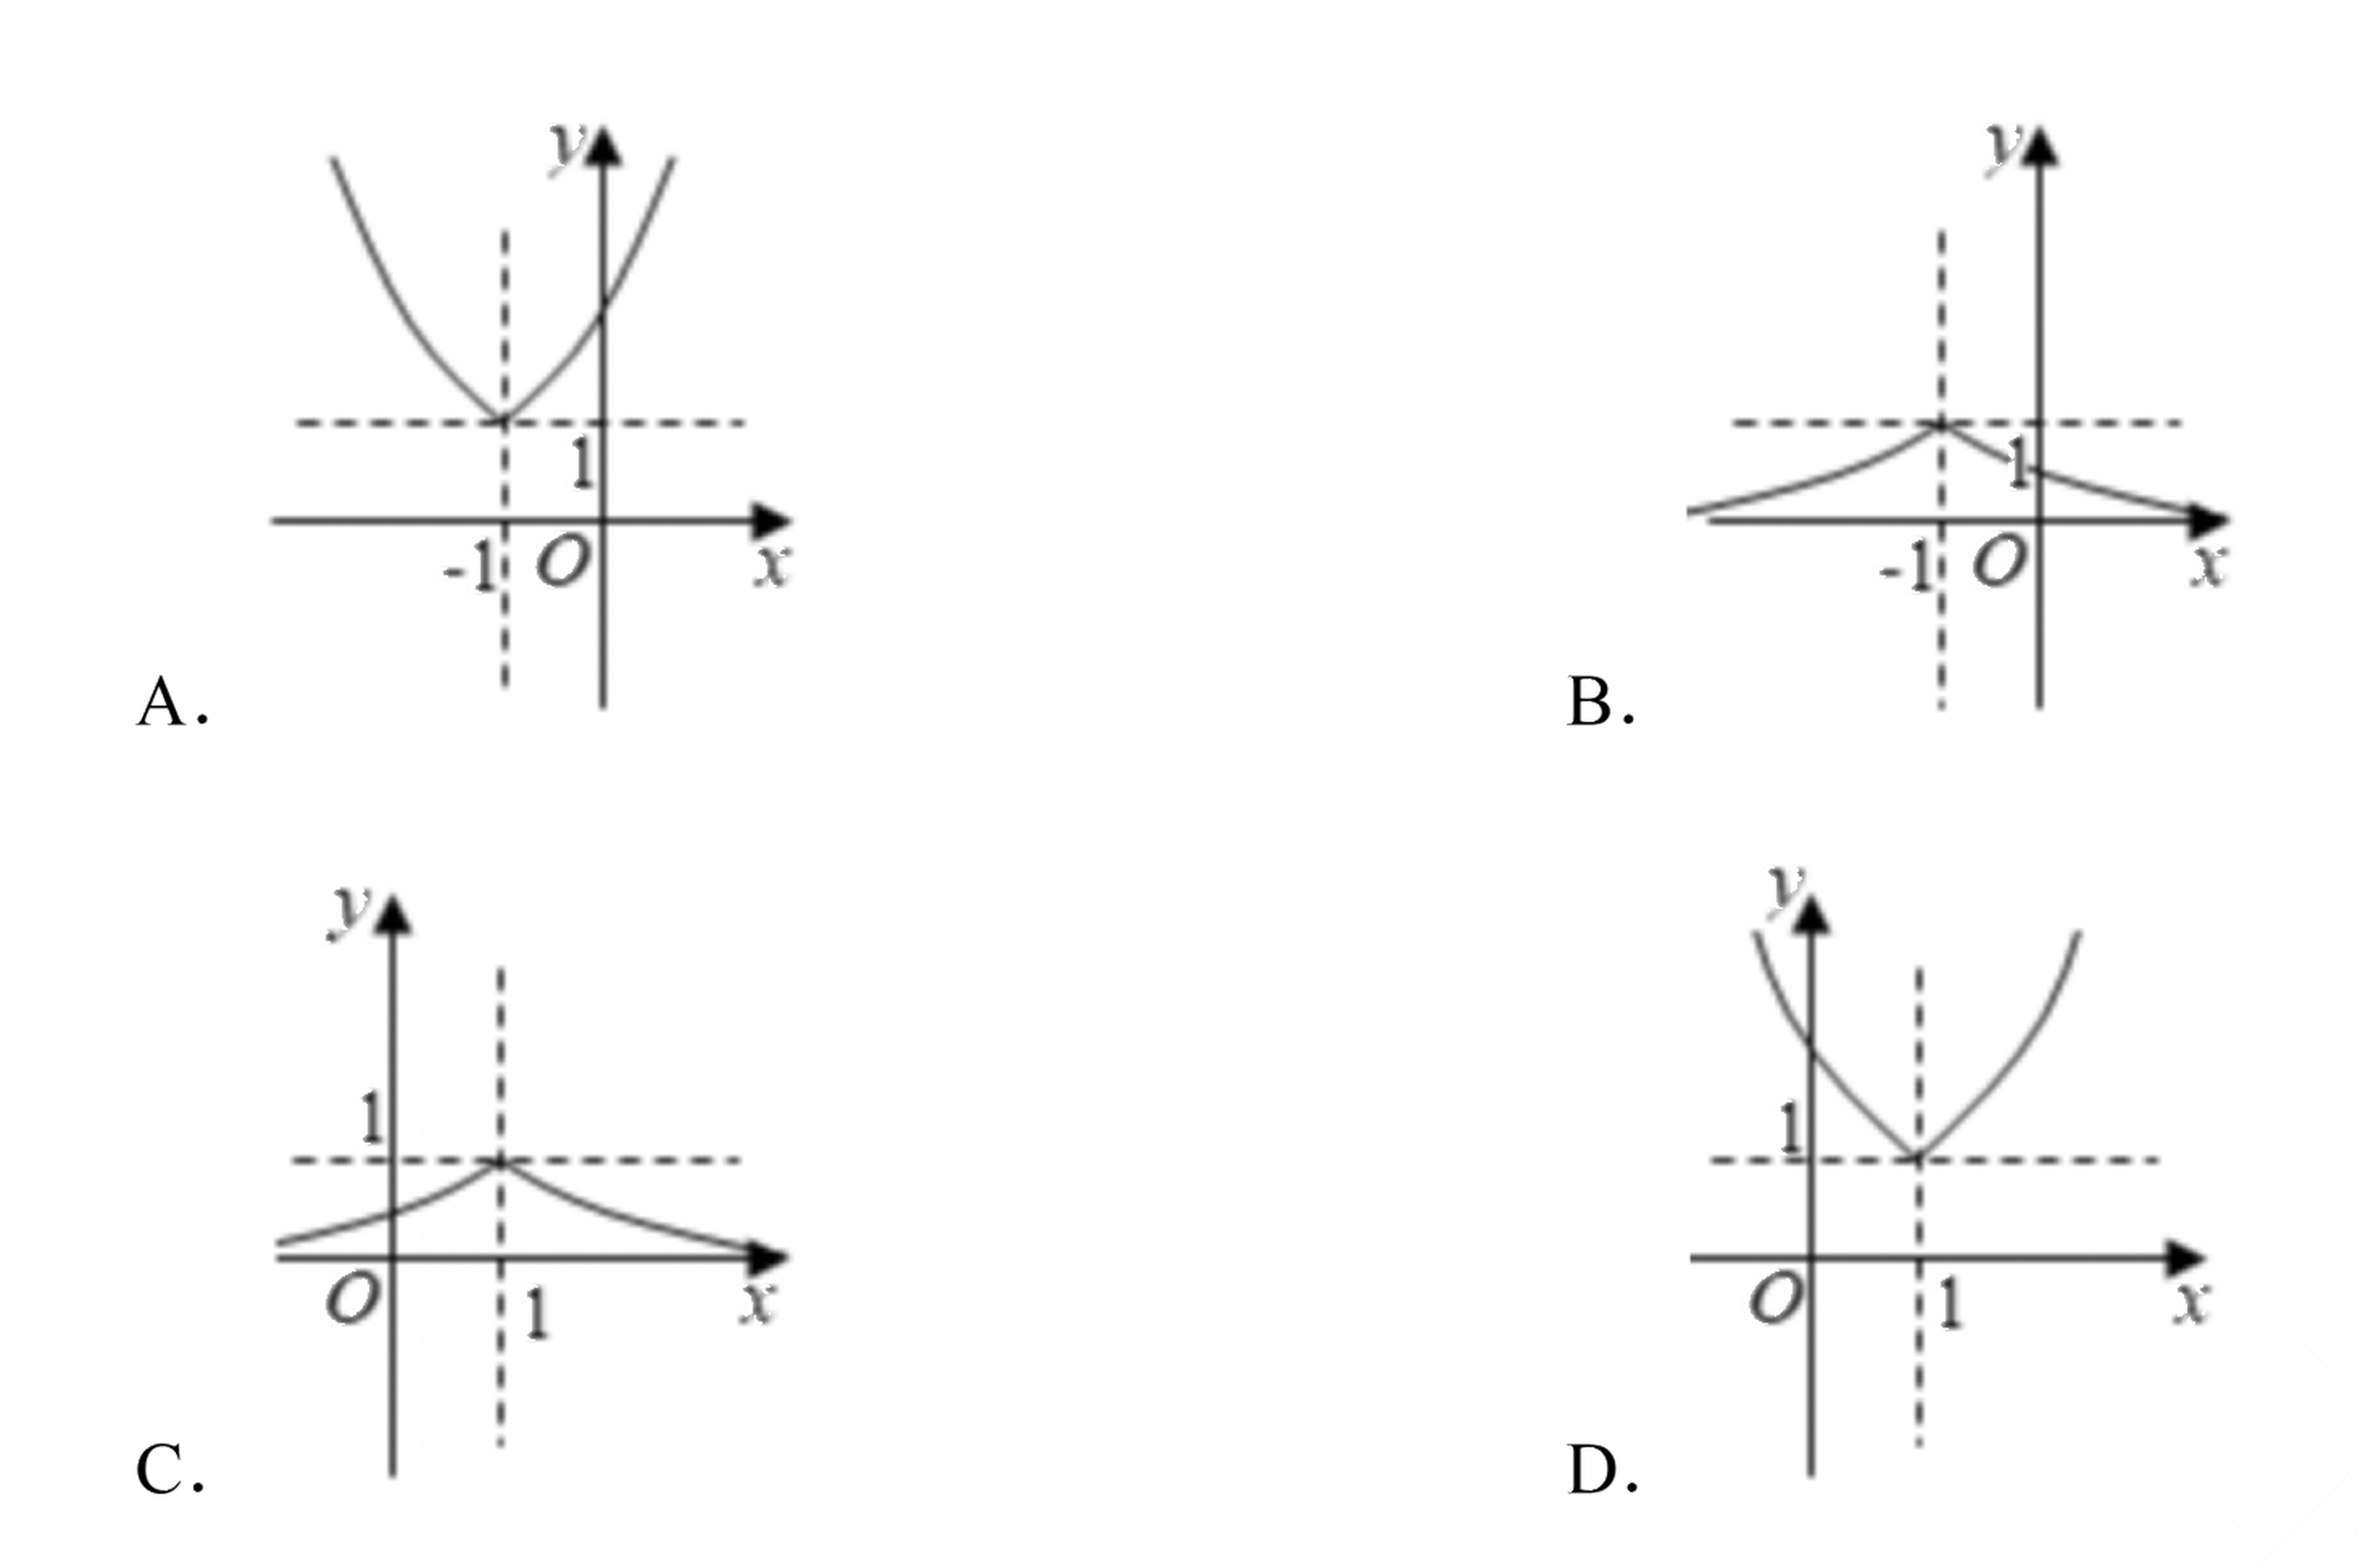
\includegraphics[width=0.80\textwidth]{figures/gao136_q22.png}
\end{center}

\ifanswer
\ans{$B$}
\fi

\end{enumerate}

\end{document}
"
% 紧凑版：xelatex "\def\iscompact{1}% 高一136_三林中学_期中.tex
%   —— 高一上数学"2026-2027 年三林中学高一上期中"（试卷版/答案版）
% 试卷版：xelatex 高一136_三林中学_期中.tex
% 答案版：xelatex "\def\isanswer{1}% 高一136_三林中学_期中.tex
%   —— 高一上数学"2026-2027 年三林中学高一上期中"（试卷版/答案版）
% 试卷版：xelatex 高一136_三林中学_期中.tex
% 答案版：xelatex "\def\isanswer{1}\input{高一136_三林中学_期中.tex}"
% 紧凑版：xelatex "\def\iscompact{1}\input{高一136_三林中学_期中.tex}"
%
% ① 原始材料：微信公众号"魔都数学加油站"文章，作者破晓，2026-11-15 18:04 发布；
% 连载"27学年高一136"，原文标题"27学年高一136——2026-2027年上海市三林中学高一上期中"；
% 原文链接：https://mp.weixin.qq.com/s/jaMzqMm6pDvcT0yM0d7eaQ。
% 正文为 7 张 PNG 页（01、04、06 为 4762x6735；02、03、05、07 为 2560x3620，
% 同一篇各页分辨率不同，逐页按各自分辨率裁图核对），题目下印有【答案】或【解析】，为讲评版。
% 题目、解析均据原图转录；卷面粉红色水印"魔都数学加油站"及公众号页脚未录入。
% 全卷 3 幅插图：第 13 题四幅坐标图选项（03 页）、第 20 题药物浓度折线/曲线图（05 页）、
% 第 22 题四幅抛物线/坐标图选项（07 页），均取原卷截图去粉色水印、去色、LANCZOS 放大，
% 四幅选项按原卷 2x2 排布合并为一张；图前按惯例加 \needvspace 守卫。
%
% 卷首标题：原卷印作"2026-2027 年三林中学高一上期中"（公众号标题中的"上海市"
% 卷面标题行没有，本稿照卷面），年份区间按全稿惯例排 en dash；原卷未印副标题，
% 本卷为期中卷、跨集合与常用逻辑用语／不等式／函数三章，按题目内容标为
% "集合与常用逻辑用语、不等式、函数"（与 125／126／128／129／131／132／133 同期中卷口径相同）：
% 集合与逻辑见 Q3、Q6、Q10、Q12、Q16、Q18、Q21，不等式见 Q5、Q7、Q8、Q9、Q14、Q15，
% 函数（幂函数、指数／对数、基本不等式应用）见 Q4、Q11、Q13、Q17、Q19、Q20、Q22。
%
% 题号体例：本卷共 20 题——一、填空题 3—12（10 题）、二、选择题 13—16（4 题）、
% 三、解答题 17—21（5 题）、四、附加题 22（1 题）。四节分别
% \setcounter{enumi}{2}／{12}／{16}／{21}。
%
% ② 与原卷的排版差异：
%   ① 原文从第 3 题起，本稿保留原题号；末节"四、附加题"另起 \bigsec，题号续到 22；
%   ② 原卷每题下直接印【答案】或【解析】，本稿按全稿惯例置于答案版；第 3、4、6 题只印
%      【答案】、无【解析】，提 \ans{}；第 14 题答案 C 印在题干括号内、无【解析】，按
%      高一53／高一108／高一132／高一133 成例括号留空、另提 \ans{$C$}；第 22 题答案 B
%      印在题干括号内、无【解析】，同例提 \ans{$B$}；第 13、15、16 题答案在解析末句
%      "故选 …"，括号内留空、不另提 \ans{}；其余各题印【解析】、无独立答案段；
%   ③ 原卷未印副标题，本稿按"知识模块"口径补出；
%   ④ 原卷填空横线按全稿惯例排为 \blankline[4.4em]；选择题括号排 \mbox{（\quad）}、
%      每个选项段前按惯例加 \keepwithprev（四幅图选项那一枚放在 \begin{center} 之前）；
%      解答题不留作答区、不加 \anspace（原卷为讲评版，与 129／131／132／133 同）；
%   ⑤ 原卷数集排斜体 $R$／$R^+$／$Z$，按全稿惯例改 \R／\R^+／\Z；空集记号 \varnothing；
%      绝对值排 \lvert…\rvert，集合描述竖线排 \mid；不等号按全稿惯例排 \leqslant／\geqslant；
%   ⑥ 子题标号 (1)(2)(3) 原卷用半角括号，照录；圈数字 ①②③④ 照录；第 12 题甲／乙／丙
%      三行与第 14 题四个编号不等式照录；
%   ⑦ 数学式内半角逗号照录（如 Q4"$a>0,a\neq1$"、Q6"$\{(-2,4),(1,1)\}$"、
%      Q7"$a=2+3=5,b=2\times3=6$"、Q11"$x_1,x_2$"、Q12"$m,n\in R^+$"、
%      Q15"$a>1,b\geq0$"、Q18"$B=(2a,a+1)$"、Q20"$4t,0\leq t\leq1$"、
%      Q21"$\{-3,-2,-1,0,1,2,3\}$"）；原卷行末西文句点照录，行中全角逗号照录；
%   ⑧ 三幅插图：第 13 题四幅坐标图选项合并裁为一张 \includegraphics（题前 \needvspace{9cm}）；
%      第 20 题折线/曲线图取 05 页截图（0.42\textwidth）；第 22 题四幅抛物线/坐标图选项合并
%      裁为一张（题前 \needvspace{9cm}）。第 13、22 题分别是"二、选择题""四、附加题"的首题
%      且带大图块，另在两处 \bigsec 之前各加 \needvspace{11cm} 连节标题一起量，避免节标题
%      孤立在页末（切页审计 B 类；照 高一26／40／59 成例）。第 20 题图不是节首题、三版试排
%      图均与题干同页，加 7cm 守卫反会多出一张只有两行正文的稀疏页，故不另加守卫；
%      三版切页审计均"合计异常：无"（试卷 4 页／紧凑 4 页／答案 6 页）；
%   ⑨ 跨页续印按题合并：Q16 题干在 03 页、括号与选项及【解析】在 04 页；Q19 题干在 04 页、
%      (2) 与【解析】在 05 页；Q20 (3)【解析】在 06 页；Q22 四幅图在 07 页；本稿按题连排；
%   ⑩ 题干中的中文弯引号按原卷照录，注释内一律 ASCII 引号；原卷"图像／图象"两种写法混用，
%      逐处照录（Q4、Q19 作"图像"，Q13、Q15、Q20、Q22 作"图象"）；
%   ⑪ 附加题节：原卷印"四、附加题"，本稿用 \bigsec{四、附加题} 另起一节、
%      \setcounter{enumi}{21}，顶层 1 个 \item（与 高一09／15／16／22／35／39／47／61 同口径）；
%      Q22 只印括号内答案、提 \ans{}，不计入 \step 账。
%
% 判别式字形：全卷仅第 9 题【解析】cases 块出现判别式"$\Delta=a^2-8a<0$"，原卷印
%   等腰、偏高的三角 $\Delta$，逐处放大核对并照录 \Delta；全卷未出现扁等边三角 \triangle。
%
% 子集符号：第 18 题 (2) 题干"$B\subseteq A$"与【解析】"$B\subseteq A$"两处原卷均印
%   带下划线 $\subseteq$，逐处放大核对、照录 \subseteq；全卷未出现单线 \subset。
%
% 原卷存疑照录（均照录未改，正文对应处另有 % 注）：
%   第 12 题乙行"$\dfrac{m+n}{mm}=\dfrac1{mn}$"前一分母印作 $mm$（后一处作 $mn$），照录；
%   第 12 题【解析】"$\geqslant\dfrac1{100}\left[a^2+1+2\sqrt{a^2}\right]$"保留 $\sqrt{a^2}$
%      未化简为 $a$，照录；
%   第 13 题【解析】"排除 BC"与"排除 D"连写选项字母，照录；
%   第 18 题 (2)【解析】末行"所以实数 $a$ 的取值范围 $(-\infty,-2]\cup[\frac12,1)$"
%      "取值范围"后脱"是／为"字，照录；
%   第 21 题 (3) 题干"求出使得集合 $B$ 中元素最少的 $k$ 的所有取值"而【解析】只给出
%      $k=-2$ 一处，措辞照录。
%
% 行数复核：逐题数 \step 条数，合计 51 条（Q3：0；Q4：0；Q5：2；Q6：0；Q7：2；Q8：1；
% Q9：1；Q10：4；Q11：1；Q12：4；Q13：2；Q14：0；Q15：2；Q16：3；Q17：1；Q18：5；
% Q19：4；Q20：7；Q21：12；Q22：0），与原卷印刷行逐题相等（cases 块作一个印刷行计）。
% 第 3、4、6、14、22 题只印【答案】、提 \ans{}，不计入 \step 账；第 13、15、16 题答案在
% 解析末句，括号内留空、不另提 \ans{}。
%
\documentclass[a4paper,11pt]{article}
\usepackage{common}

\begin{document}

\examtitlest[3]{2026--2027 年三林中学高一上期中}{集合与常用逻辑用语、不等式、函数}

\bigsec{一、填空题}

\begin{enumerate}
\setcounter{enumi}{2}

\item 用反证法证明命题“若 $x+y\neq5$，则 $x\neq2$ 或 $y\neq3$”为真命题时，第一个步骤是\blankline[4.4em].

\ifanswer
\ans{假设 $x=2$ 且 $y=3$}
\fi

\item 函数 $y=a^{x-1}+1(a>0,a\neq1)$ 的图像恒过定点 $A$，则点的坐标是\blankline[4.4em].

\ifanswer
\ans{$(1,2)$}
\fi

\item 已知 $x>1$，则 $x+\dfrac4{x-1}$ 的最小值是\blankline[4.4em].

\ifanswer
\solbegin
\step{由 $x>1$，得 $x-1>0$，则 $x+\dfrac4{x-1}=x-1+\dfrac4{x-1}+1\geqslant2\sqrt{(x-1)\cdot\dfrac4{x-1}}+1=5$，}
\step{当且仅当 $x-1=\dfrac4{x-1}$ 即 $x=3$ 时取等号，取得最小值 $5$.}
\solend
\fi

\item 已知集合 $A=\{(x,y)\mid y=x^2\}$，集合 $B=\{(x,y)\mid y=2-x\}$，求 $A\cap B=$\blankline[4.4em].

\ifanswer
\ans{$\{(-2,4),(1,1)\}$}
\fi

\item 已知一元二次不等式 $x^2-ax+b<0$ 的解集为 $(2,3)$，则不等式 $bx^2-ax+1>0$ 的解集是\blankline[4.4em].

\ifanswer
\solbegin
\step{$a=2+3=5,b=2\times3=6$，则 $bx^2-ax+1>0$ 即 $6x^2-5x+1>0$，}
\step{即 $(3x-1)(2x-1)>0$，解集为 $\left(-\infty,\dfrac13\right)\cup\left(\dfrac12,+\infty\right)$.}
\solend
\fi

\item 不等式 $(x+2)^3<(5-2x)^3$ 的解集为\blankline[4.4em].

\ifanswer
\solbegin
\step{由 $(x+2)^3<(5-2x)^3$ 得 $x+2<5-2x$，故解集为 $(-\infty,1)$.}
\solend
\fi

\item 若关于 $x$ 的不等式 $ax^2-ax+2>0$ 的解集为 $\R$，则实数 $a$ 的取值范围是\blankline[4.4em].

\ifanswer
\solbegin
\step{由题意得 $a=0$ 或 $\begin{cases}a>0\\\Delta=a^2-8a<0\end{cases}$，所以 $0\leqslant a<8$.}% 判别式原卷印高三角 $\Delta$，照录
\solend
\fi

\item 已知关于 $x$ 的不等式 $\lvert x+3\rvert+\lvert x-a\rvert\geqslant5$ 恒成立，则实数 $a$ 的取值范围为\blankline[4.4em].

\ifanswer
\solbegin
\step{因为 $\lvert x+3\rvert+\lvert x-a\rvert\geqslant\lvert x-a-x-3\rvert=\lvert 3+a\rvert$，}
\step{要使 $\lvert x+3\rvert+\lvert x-a\rvert\geqslant5$ 恒成立，则 $\lvert a+3\rvert\geqslant5$ 即可，}
\step{所以 $a+3\geqslant5$ 或 $a+3\leqslant-5$，解得 $a\geqslant2$ 或 $a\leqslant-8$，}
\step{即实数 $a$ 的取值范围是 $(-\infty,-8]\cup[2,+\infty)$.}
\solend
\fi

\item 若方程 $\lg^2 x-2\lg x-2=0$ 的两个解为 $x_1,x_2$，求 $\log_{x_1}x_2+\log_{x_2}x_1$ 的值为\blankline[4.4em].

\ifanswer
\solbegin
\step{$\log_{x_1}x_2+\log_{x_2}x_1=\dfrac{\lg x_2}{\lg x_1}+\dfrac{\lg x_1}{\lg x_2}=\dfrac{(\lg x_1+\lg x_2)^2-2\lg x_1\lg x_2}{\lg x_1\lg x_2}=-4$.}
\solend
\fi

\item 三个同学对问题“已知 $m,n\in \R^+$，且 $m+n=1$，求 $\dfrac1m+\dfrac1n$ 的最小值”提出各自的解题思路：

思路：

甲：$\dfrac1m+\dfrac1n=\dfrac{m+n}{m}+\dfrac{m+n}{n}=2+\dfrac nm+\dfrac mn$，可用基本不等式求解；

乙：$\dfrac1m+\dfrac1n=\dfrac{m+n}{mm}=\dfrac1{mn}=\dfrac1{m(1-m)}$，可用二次函数配方法求解；% 原卷前一分母印作 $mm$，照录

丙：$\dfrac1m+\dfrac1n=\left(\dfrac1m+\dfrac1n\right)(m+n)=2+\dfrac nm+\dfrac mn$，可用基本不等式求解；参考上述解题思路，

可求得当 $x=$\blankline[4.4em]时，$y=\dfrac{a^2}{x^2}+\dfrac1{100-x^2}$（$0<x<10$，$a>0$）有最小值.

\ifanswer
\solbegin
\step{$y=\dfrac{a^2}{x^2}+\dfrac1{100-x^2}=\left(\dfrac{a^2}{x^2}+\dfrac1{100-x^2}\right)[x^2+(100-x^2)]\times\dfrac1{100}$}
\step{$=\dfrac1{100}\left[a^2+1+\dfrac{x^2}{100-x^2}+\dfrac{a^2(100-x^2)}{x^2}\right]\geqslant\dfrac1{100}\left[a^2+1+2\sqrt{a^2}\right]$}% 原卷保留 $\sqrt{a^2}$ 未化简，照录
\step{当且仅当 $\dfrac{x^2}{100-x^2}=\dfrac{a^2(100-x^2)}{x^2}$，即 $x=\sqrt{\dfrac{100a}{a+1}}$ 时，}
\step{$y=\dfrac{a^2}{x^2}+\dfrac1{100-x^2}(0<x<10,a>0)$ 有最小值.}
\solend
\fi

\end{enumerate}

% 第 13 题是"二、选择题"首题且带 9cm 图块，守卫须放在 \bigsec 之前连节标题一起量，
% 否则"二、选择题"会孤立在页末（B 类，照 高一26／40／59 成例）
\needvspace{11cm}
\bigsec{二、选择题}

\begin{enumerate}
\setcounter{enumi}{12}

% 第 13 题四幅坐标图选项是一整块，守卫放在 \item 之前
\needvspace{9cm}
\item 下列图象中，最符合函数 $y=x^{\frac54}$ 的图象的是\mbox{（\quad）}

\keepwithprev
\begin{center}
% 四幅坐标图选项取原卷 03 页截图去粉色水印，按原卷 2x2 排布合并为一张
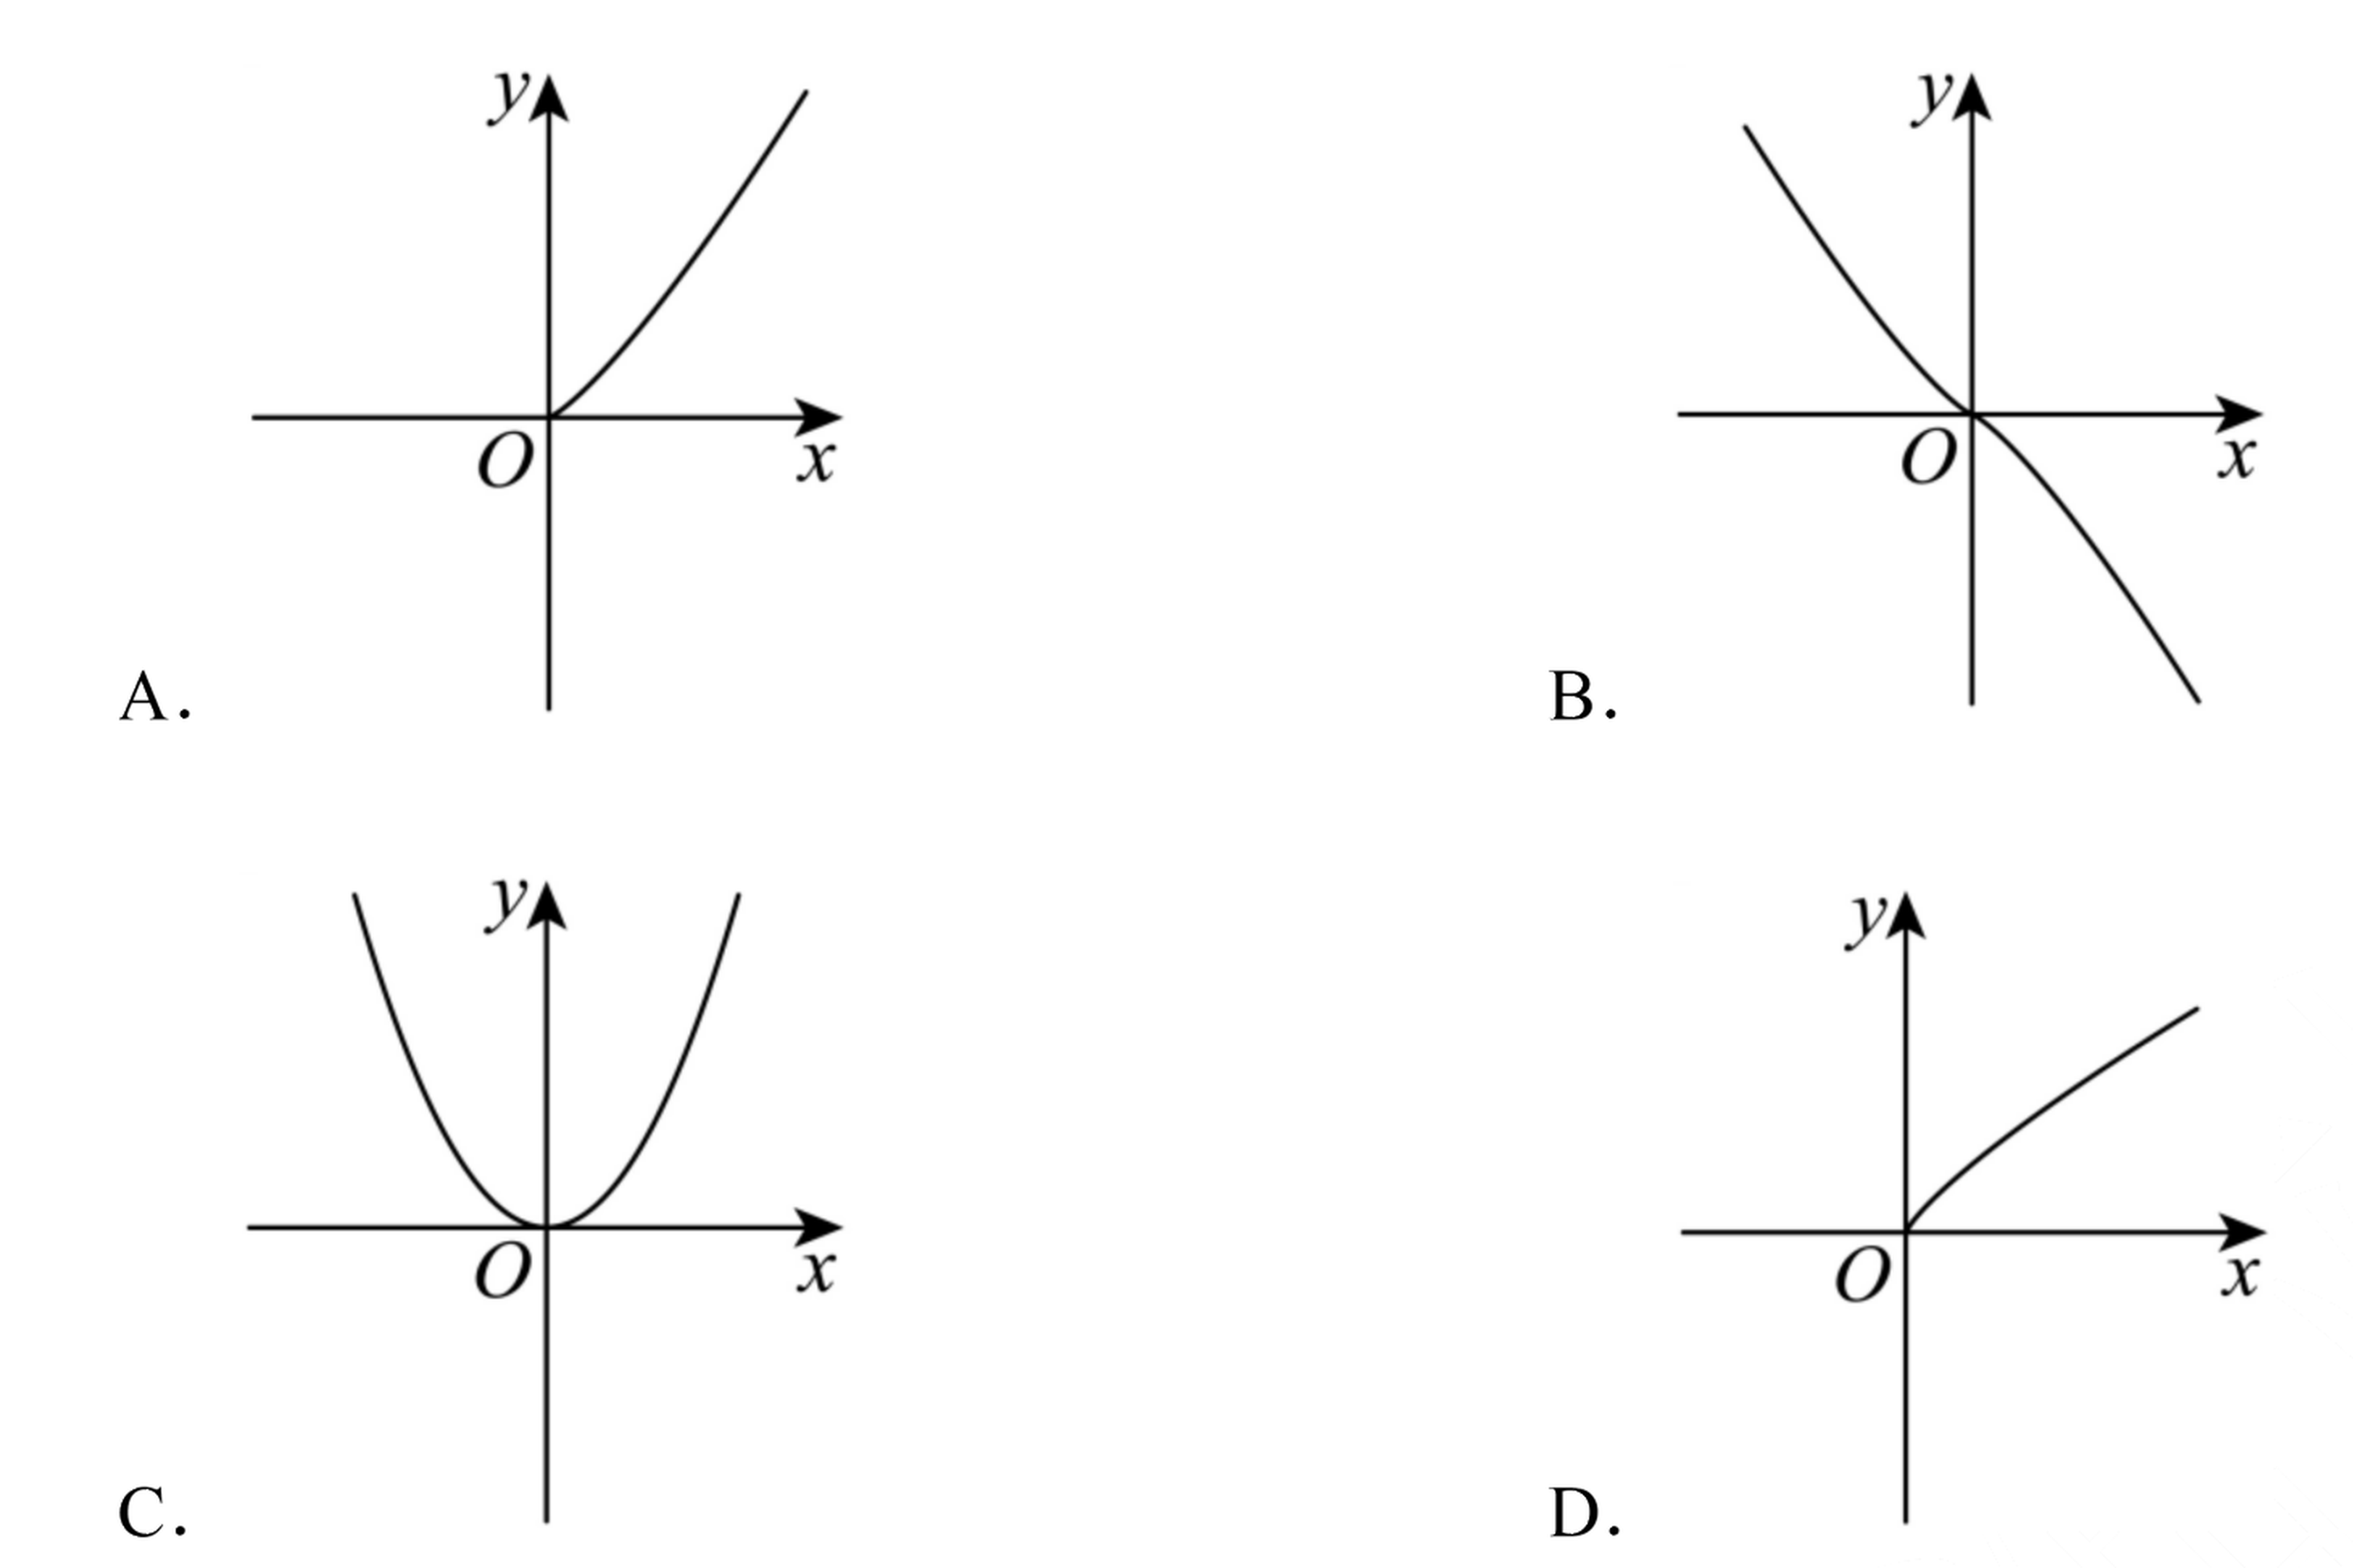
\includegraphics[width=0.80\textwidth]{figures/gao136_q13.png}
\end{center}

\ifanswer
\solbegin
\step{由 $y=x^{\frac54}=\sqrt[4]{x^5}$，函数的定义域为 $[0,+\infty)$，排除 BC，}% 原卷"排除 BC"连写，照录
\step{因为 $\dfrac54>1$，所以函数 $y=x^{\frac54}$ 的图象呈现下凸的趋势，排除 D. 故选 $A$.}
\solend
\fi

\item 下列不等式① $a+\dfrac1a\geqslant2$；② $a^2+4\geqslant4a$；③ $\left\lvert\dfrac ba+\dfrac ab\right\rvert\geqslant2$；④ $\dfrac{2a^2b^2}{a^2+b^2}\leqslant ab$；其中恒成立的是\mbox{（\quad）}

\keepwithprev
A. ①④\qquad B. ③④\qquad C. ②③\qquad D. ①②

\ifanswer
\ans{$C$}
\fi

\item 函数 $y=a^x+b-1(a>0,a\neq1)$ 单调递增且图象不经过第四象限，则 $a,b$ 满足的条件为\mbox{（\quad）}

\keepwithprev
A. $a>1,b\leqslant1$\qquad B. $a>1,b\geqslant0$\qquad C. $0<a<1,b\leqslant1$\qquad D. $0<a<1,b\geqslant1$

\ifanswer
\solbegin
\step{因为函数 $y=a^x+b-1$ 单调递增，所以 $a>1$，}
\step{图象不经过第四象限，则 $x=0$ 时，$y=b\geqslant0$，所以 $a>1,b\geqslant0$，故选 $B$.}
\solend
\fi

\item 设关于 $x$ 的不等式 $\dfrac{ax-1}{x^2-a}<0$ 的解集为 $S$，且 $3\in S$，$4\notin S$，则实数 $a$ 的取值范围为\mbox{（\quad）}

\keepwithprev
A. $(-\infty,-\sqrt3)\cup\left(\dfrac13,\sqrt3\right)$\qquad B. $\left(-\infty,\dfrac14\right)\cup(16,+\infty)$

C. $\left[\dfrac14,\dfrac13\right)\cup(9,16]$\qquad D. 不能确定

\ifanswer
\solbegin
\step{若 $3\in S$，则 $\dfrac{3a-1}{9-a}<0$，解得 $a\in\left(-\infty,\dfrac13\right)\cup(9,+\infty)$，}
\step{若 $4\notin S$，则 $16-a=0$ 或 $\dfrac{4a-1}{16-a}\geqslant0$，解得 $a\in\left[\dfrac14,16\right]$，}
\step{故实数 $a$ 的取值范围为 $\left[\dfrac14,\dfrac13\right)\cup(9,16]$，故选 $C$.}
\solend
\fi

\end{enumerate}

\bigsec{三、解答题}

\begin{enumerate}
\setcounter{enumi}{16}

\item 计算：(1) 计算 $\dfrac{\lg8+\lg125-\lg2-\lg5}{\lg\sqrt{10}\cdot\lg0.1}$；(2) 若 $a^{2x}=2(a>0)$，求 $\dfrac{a^{3x}+a^{-3x}}{a^x+a^{-x}}$.

\ifanswer
\solbegin
\step{(1) 原式 $=\dfrac{2-1}{\frac12\cdot(-1)}=-2$；(2) 原式 $=a^{2x}-1+a^{-2x}=2-1+\dfrac12=\dfrac32$.}
\solend
\fi

\item 不等式 $\dfrac{x-1}{x+1}\geqslant0$ 的解集为 $A$，不等式 $(x-a-1)(2a-x)>0(a<1)$ 的解集为 $B$.

(1) 求集合 $A$；

(2) 若 $B\subseteq A$，求实数 $a$ 的取值范围.

\ifanswer
\solbegin
\step{(1) $A=(-\infty,-1)\cup[1,+\infty)$.}
\step{(2) 由 $(x-a-1)(2a-x)>0(a<1)$，得 $(x-a-1)(x-2a)<0(a<1)$，}
\step{因为 $a<1$，所以 $a+1>2a$，所以 $B=(2a,a+1)$，}
\step{因为 $B\subseteq A$，所以 $2a\geqslant1$ 或 $a+1\leqslant-1$，即 $a\geqslant\dfrac12$ 或 $a\leqslant-2$，}
\step{而 $a<1$，所以实数 $a$ 的取值范围 $(-\infty,-2]\cup\left[\dfrac12,1\right)$.}% 原卷"取值范围"后脱"是／为"，照录
\solend
\fi

\item 已知幂函数 $y=x^m(m\in\R)$ 经过点 $\left(4,\dfrac12\right)$.

(1) 求此幂函数的表达式和定义域；

(2) 已知点 $A(a+2,y_1)$，点 $B(3-2a,y_2)(a\in\R)$ 在此幂函数的图像上，且满足 $y_1<y_2$，求实数 $a$ 的取值范围.

\ifanswer
\solbegin
\step{(1) 幂函数 $y=x^m(m\in\R)$ 经过点 $\left(4,\dfrac12\right)$，所以 $4^m=\dfrac12\Rightarrow m=-\dfrac12$，}
\step{所以 $f(x)=x^{-\frac12}$，定义域为 $(0,+\infty)$.}
\step{(2) 由于函数 $f(x)$ 在其定义域 $(0,+\infty)$ 上严格减，}
\step{由 $y_1<y_2$，得 $a+2>3-2a\geqslant0\Rightarrow a\in\left(\dfrac13,\dfrac32\right]$.}
\solend
\fi

% 第 20 题图取 05 页截图（0.42\textwidth、高约 6cm）。试排 \item 前加 7cm 守卫会多出
% 一张只有两行正文的稀疏页，且三版不加守卫时图均与题干、【解析】同页，故不另加守卫
\item 某医药研究所开发一种抗甲流新药，如果成年人按规定的剂量服用，据监测：服药后每毫升血液中的含药量 $y$（微克）与时间 $t$（小时）之间近似满足如图所示的曲线.

(1) 结合图，求 $k$ 与 $a$ 的值；

(2) 写出服药后 $y$ 与 $t$ 之间的函数关系式 $y=f(t)$；

(3) 据进一步测定：每毫升血液中含药量不少于 $0.5$ 微克时治疗疾病有效，求服药一次治疗有效的时间范围？

\begin{center}
% 图取原卷 05 页截图去粉色水印、去色，3x LANCZOS 放大
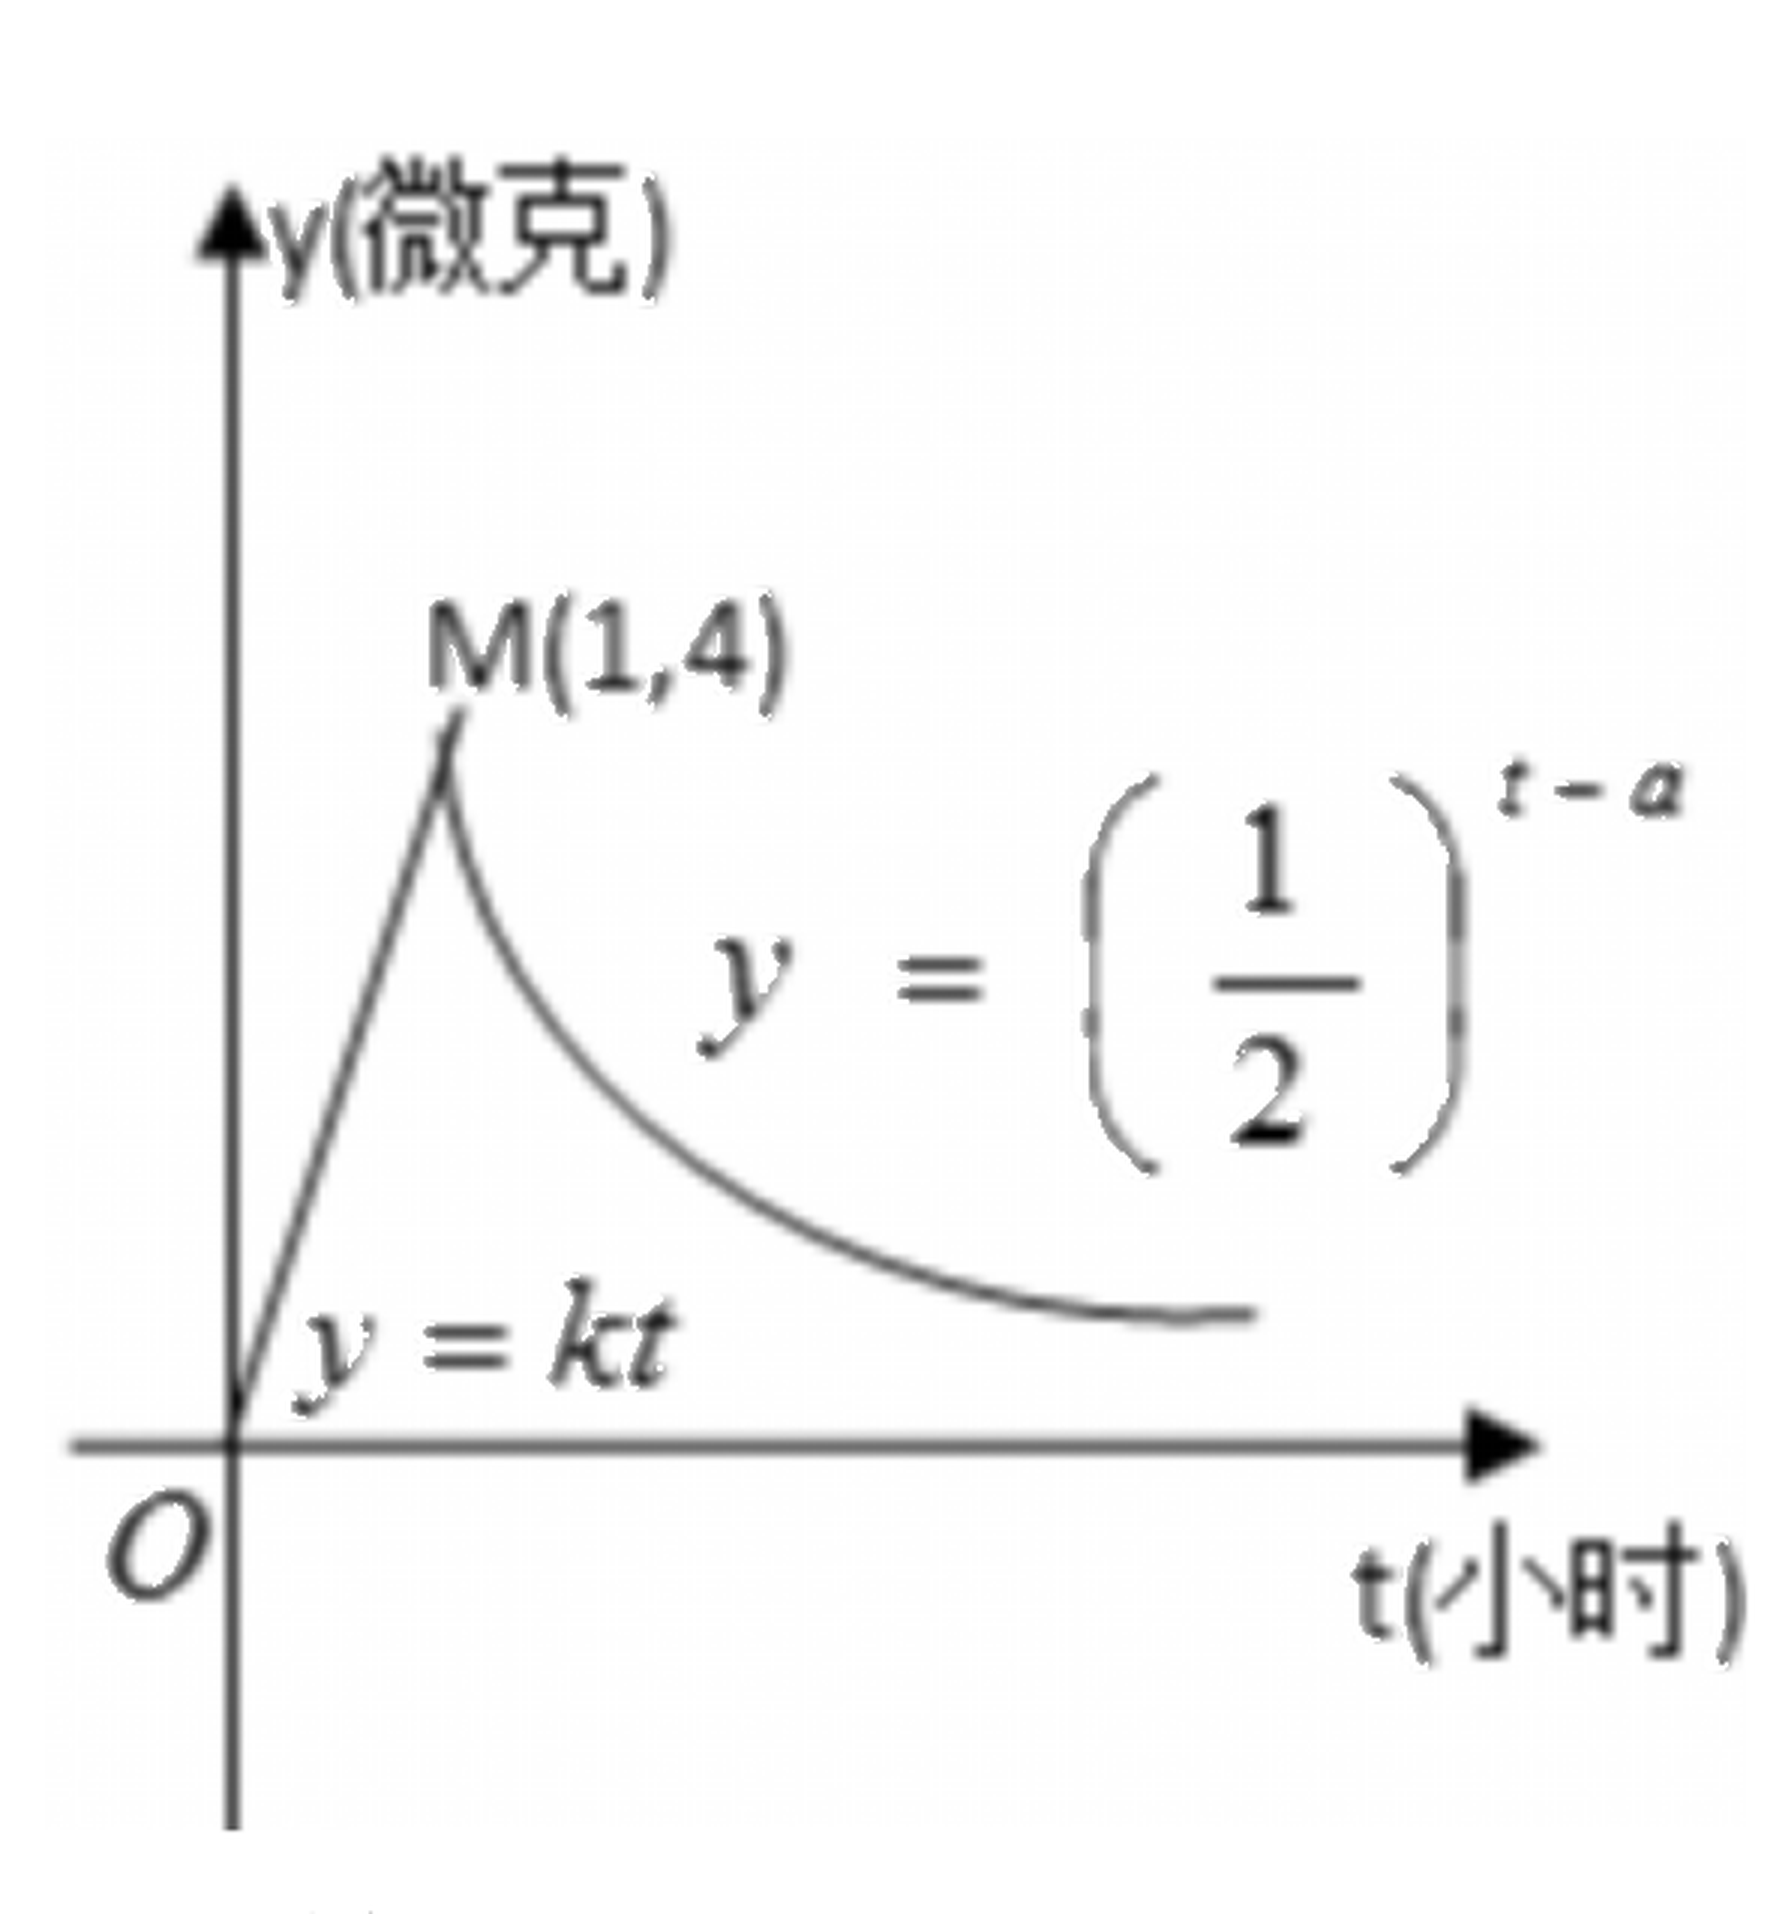
\includegraphics[width=0.42\textwidth]{figures/gao136_q20.png}
\end{center}

\ifanswer
\solbegin
\step{(1) 当 $0\leqslant t\leqslant1$ 时，函数图象是一条线段，由于过原点与点 $(1,4)$，所以 $k=4$，}
\step{其解析式为 $y=4t$，$0\leqslant t\leqslant1$；}
\step{当 $t\geqslant1$ 时，函数的解析式为 $y=\left(\dfrac12\right)^{t-a}$，}
\step{此时 $M(1,4)$ 在曲线上，将此点的坐标代入函数解析式得 $4=\left(\dfrac12\right)^{1-a}$，}
\step{解得 $a=3$；}
\step{(2) 由 (1) 得 $f(t)=\begin{cases}4t,0\leqslant t\leqslant1\\\left(\frac12\right)^{t-3},t>1\end{cases}$；}
\step{(3) 由 (2) 得，令 $f(t)\geqslant0.5$，即 $\begin{cases}4t\geqslant0.5,0\leqslant t\leqslant1\\\left(\frac12\right)^{t-3}\geqslant0.5,t>1\end{cases}$，所以 $\dfrac18\leqslant t\leqslant4$.}
\solend
\fi

\item 已知关于 $x$ 的不等式 $(kx-k^2-4)(x-4)>0$，其中 $k\in\R$.

(1) 当 $k=-1$，求不等式的解集 $A$；

(2) 当 $k$ 变化时，试求不等式的解集 $A$；

(3) 对于不等式解集 $A$，满足 $A\cap\Z=B$. 试探究集合 $B$ 能否为有限集，若能，求出使得集合 $B$ 中元素最少的 $k$ 的所有取值，并用列举法表示此时的集合 $B$，若不能，说明理由；

\ifanswer
\solbegin
\step{(1) 当 $k=-1$ 时，原不等式可化为 $(x+5)(x-4)<0$，}
\step{解得 $-5<x<4$，故不等式的解集为 $\{x\mid -5<x<4\}$；}
\step{(2) 当 $k=0$ 时，解集为 $\{x\mid x<4\}$，}
\step{当 $k>0$ 时，$\dfrac{k^2+4}{k}=k+\dfrac4k\geqslant4$，解集为 $\{x\mid x<4\text{ 或 }x>\dfrac{k^2+4}{k}\}$；}
\step{当 $k<0$ 时，解集为 $\{x\mid \dfrac{k^2+4}{k}<x<4\}$，}
\step{综上，当 $k=0$ 时，$A=\{x\mid x<4\}$，}
\step{当 $k>0$ 时，$A=\{x\mid x<4\text{ 或 }x>\dfrac{k^2+4}{k}\}$；}
\step{当 $k<0$ 时，$A=\{x\mid \dfrac{k^2+4}{k}<x<4\}$，}
\step{(3) 由 (2) 得当 $k\geqslant0$ 时，$B$ 为无限集，当 $k<0$ 时，$B$ 为有限集，}
\step{此时，$\dfrac{k^2+4}{k}=k+\dfrac4k\leqslant-4$，当且仅当 $k=-2$ 时取等号，}
\step{所以 $k=-2$ 时，$B$ 中元素最少，此时 $A=\{x\mid -4<x<4\}$，}
\step{所以 $B=\{-3,-2,-1,0,1,2,3\}$.}
\solend
\fi

\end{enumerate}

% 第 22 题是"四、附加题"首题且带 9cm 图块，守卫须放在 \bigsec 之前连节标题一起量，
% 否则"四、附加题"会孤立在页末（B 类，照 高一26／40／59 成例）
\needvspace{11cm}
\bigsec{四、附加题}

\begin{enumerate}
\setcounter{enumi}{21}

% 第 22 题四幅抛物线/坐标图选项是一整块，守卫放在 \item 之前
\needvspace{9cm}
\item 函数 $f(x)=\left(\dfrac12\right)^{\lvert x+1\rvert}$ 的图象大致为\mbox{（\quad）}

\keepwithprev
\begin{center}
% 四幅抛物线/坐标图选项取原卷 07 页截图去粉色水印，按原卷 2x2 排布合并为一张
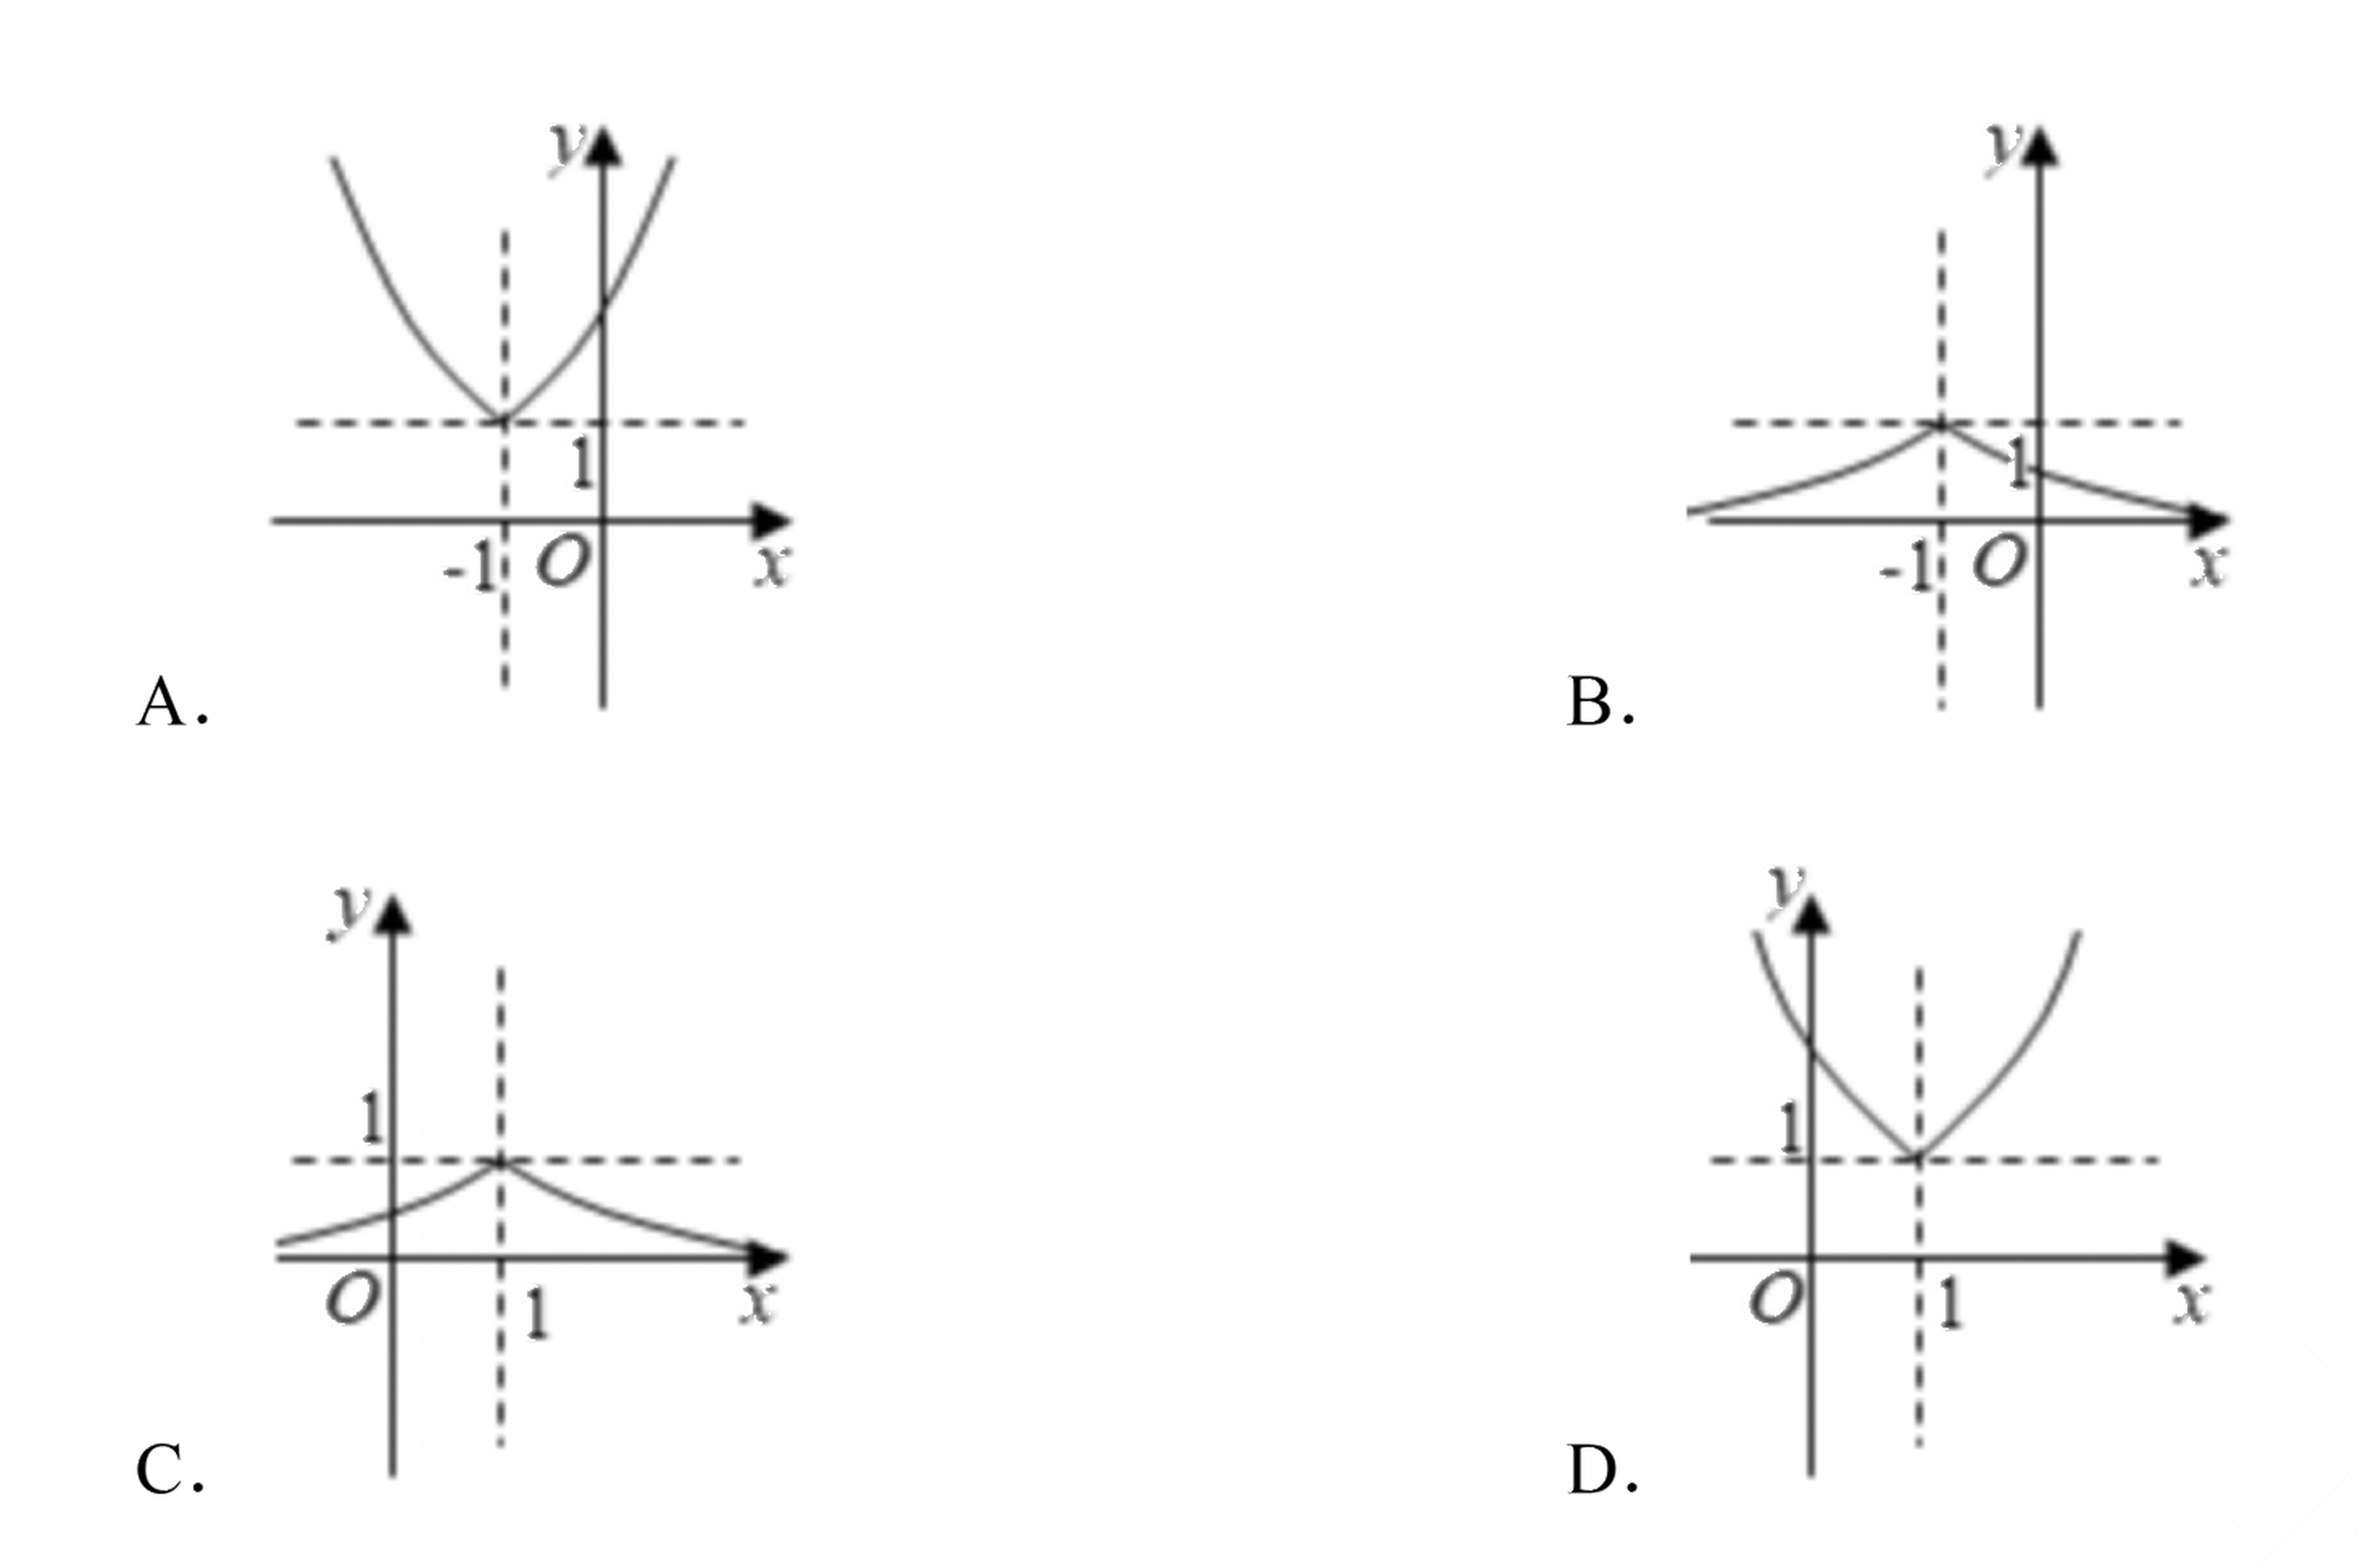
\includegraphics[width=0.80\textwidth]{figures/gao136_q22.png}
\end{center}

\ifanswer
\ans{$B$}
\fi

\end{enumerate}

\end{document}
"
% 紧凑版：xelatex "\def\iscompact{1}% 高一136_三林中学_期中.tex
%   —— 高一上数学"2026-2027 年三林中学高一上期中"（试卷版/答案版）
% 试卷版：xelatex 高一136_三林中学_期中.tex
% 答案版：xelatex "\def\isanswer{1}\input{高一136_三林中学_期中.tex}"
% 紧凑版：xelatex "\def\iscompact{1}\input{高一136_三林中学_期中.tex}"
%
% ① 原始材料：微信公众号"魔都数学加油站"文章，作者破晓，2026-11-15 18:04 发布；
% 连载"27学年高一136"，原文标题"27学年高一136——2026-2027年上海市三林中学高一上期中"；
% 原文链接：https://mp.weixin.qq.com/s/jaMzqMm6pDvcT0yM0d7eaQ。
% 正文为 7 张 PNG 页（01、04、06 为 4762x6735；02、03、05、07 为 2560x3620，
% 同一篇各页分辨率不同，逐页按各自分辨率裁图核对），题目下印有【答案】或【解析】，为讲评版。
% 题目、解析均据原图转录；卷面粉红色水印"魔都数学加油站"及公众号页脚未录入。
% 全卷 3 幅插图：第 13 题四幅坐标图选项（03 页）、第 20 题药物浓度折线/曲线图（05 页）、
% 第 22 题四幅抛物线/坐标图选项（07 页），均取原卷截图去粉色水印、去色、LANCZOS 放大，
% 四幅选项按原卷 2x2 排布合并为一张；图前按惯例加 \needvspace 守卫。
%
% 卷首标题：原卷印作"2026-2027 年三林中学高一上期中"（公众号标题中的"上海市"
% 卷面标题行没有，本稿照卷面），年份区间按全稿惯例排 en dash；原卷未印副标题，
% 本卷为期中卷、跨集合与常用逻辑用语／不等式／函数三章，按题目内容标为
% "集合与常用逻辑用语、不等式、函数"（与 125／126／128／129／131／132／133 同期中卷口径相同）：
% 集合与逻辑见 Q3、Q6、Q10、Q12、Q16、Q18、Q21，不等式见 Q5、Q7、Q8、Q9、Q14、Q15，
% 函数（幂函数、指数／对数、基本不等式应用）见 Q4、Q11、Q13、Q17、Q19、Q20、Q22。
%
% 题号体例：本卷共 20 题——一、填空题 3—12（10 题）、二、选择题 13—16（4 题）、
% 三、解答题 17—21（5 题）、四、附加题 22（1 题）。四节分别
% \setcounter{enumi}{2}／{12}／{16}／{21}。
%
% ② 与原卷的排版差异：
%   ① 原文从第 3 题起，本稿保留原题号；末节"四、附加题"另起 \bigsec，题号续到 22；
%   ② 原卷每题下直接印【答案】或【解析】，本稿按全稿惯例置于答案版；第 3、4、6 题只印
%      【答案】、无【解析】，提 \ans{}；第 14 题答案 C 印在题干括号内、无【解析】，按
%      高一53／高一108／高一132／高一133 成例括号留空、另提 \ans{$C$}；第 22 题答案 B
%      印在题干括号内、无【解析】，同例提 \ans{$B$}；第 13、15、16 题答案在解析末句
%      "故选 …"，括号内留空、不另提 \ans{}；其余各题印【解析】、无独立答案段；
%   ③ 原卷未印副标题，本稿按"知识模块"口径补出；
%   ④ 原卷填空横线按全稿惯例排为 \blankline[4.4em]；选择题括号排 \mbox{（\quad）}、
%      每个选项段前按惯例加 \keepwithprev（四幅图选项那一枚放在 \begin{center} 之前）；
%      解答题不留作答区、不加 \anspace（原卷为讲评版，与 129／131／132／133 同）；
%   ⑤ 原卷数集排斜体 $R$／$R^+$／$Z$，按全稿惯例改 \R／\R^+／\Z；空集记号 \varnothing；
%      绝对值排 \lvert…\rvert，集合描述竖线排 \mid；不等号按全稿惯例排 \leqslant／\geqslant；
%   ⑥ 子题标号 (1)(2)(3) 原卷用半角括号，照录；圈数字 ①②③④ 照录；第 12 题甲／乙／丙
%      三行与第 14 题四个编号不等式照录；
%   ⑦ 数学式内半角逗号照录（如 Q4"$a>0,a\neq1$"、Q6"$\{(-2,4),(1,1)\}$"、
%      Q7"$a=2+3=5,b=2\times3=6$"、Q11"$x_1,x_2$"、Q12"$m,n\in R^+$"、
%      Q15"$a>1,b\geq0$"、Q18"$B=(2a,a+1)$"、Q20"$4t,0\leq t\leq1$"、
%      Q21"$\{-3,-2,-1,0,1,2,3\}$"）；原卷行末西文句点照录，行中全角逗号照录；
%   ⑧ 三幅插图：第 13 题四幅坐标图选项合并裁为一张 \includegraphics（题前 \needvspace{9cm}）；
%      第 20 题折线/曲线图取 05 页截图（0.42\textwidth）；第 22 题四幅抛物线/坐标图选项合并
%      裁为一张（题前 \needvspace{9cm}）。第 13、22 题分别是"二、选择题""四、附加题"的首题
%      且带大图块，另在两处 \bigsec 之前各加 \needvspace{11cm} 连节标题一起量，避免节标题
%      孤立在页末（切页审计 B 类；照 高一26／40／59 成例）。第 20 题图不是节首题、三版试排
%      图均与题干同页，加 7cm 守卫反会多出一张只有两行正文的稀疏页，故不另加守卫；
%      三版切页审计均"合计异常：无"（试卷 4 页／紧凑 4 页／答案 6 页）；
%   ⑨ 跨页续印按题合并：Q16 题干在 03 页、括号与选项及【解析】在 04 页；Q19 题干在 04 页、
%      (2) 与【解析】在 05 页；Q20 (3)【解析】在 06 页；Q22 四幅图在 07 页；本稿按题连排；
%   ⑩ 题干中的中文弯引号按原卷照录，注释内一律 ASCII 引号；原卷"图像／图象"两种写法混用，
%      逐处照录（Q4、Q19 作"图像"，Q13、Q15、Q20、Q22 作"图象"）；
%   ⑪ 附加题节：原卷印"四、附加题"，本稿用 \bigsec{四、附加题} 另起一节、
%      \setcounter{enumi}{21}，顶层 1 个 \item（与 高一09／15／16／22／35／39／47／61 同口径）；
%      Q22 只印括号内答案、提 \ans{}，不计入 \step 账。
%
% 判别式字形：全卷仅第 9 题【解析】cases 块出现判别式"$\Delta=a^2-8a<0$"，原卷印
%   等腰、偏高的三角 $\Delta$，逐处放大核对并照录 \Delta；全卷未出现扁等边三角 \triangle。
%
% 子集符号：第 18 题 (2) 题干"$B\subseteq A$"与【解析】"$B\subseteq A$"两处原卷均印
%   带下划线 $\subseteq$，逐处放大核对、照录 \subseteq；全卷未出现单线 \subset。
%
% 原卷存疑照录（均照录未改，正文对应处另有 % 注）：
%   第 12 题乙行"$\dfrac{m+n}{mm}=\dfrac1{mn}$"前一分母印作 $mm$（后一处作 $mn$），照录；
%   第 12 题【解析】"$\geqslant\dfrac1{100}\left[a^2+1+2\sqrt{a^2}\right]$"保留 $\sqrt{a^2}$
%      未化简为 $a$，照录；
%   第 13 题【解析】"排除 BC"与"排除 D"连写选项字母，照录；
%   第 18 题 (2)【解析】末行"所以实数 $a$ 的取值范围 $(-\infty,-2]\cup[\frac12,1)$"
%      "取值范围"后脱"是／为"字，照录；
%   第 21 题 (3) 题干"求出使得集合 $B$ 中元素最少的 $k$ 的所有取值"而【解析】只给出
%      $k=-2$ 一处，措辞照录。
%
% 行数复核：逐题数 \step 条数，合计 51 条（Q3：0；Q4：0；Q5：2；Q6：0；Q7：2；Q8：1；
% Q9：1；Q10：4；Q11：1；Q12：4；Q13：2；Q14：0；Q15：2；Q16：3；Q17：1；Q18：5；
% Q19：4；Q20：7；Q21：12；Q22：0），与原卷印刷行逐题相等（cases 块作一个印刷行计）。
% 第 3、4、6、14、22 题只印【答案】、提 \ans{}，不计入 \step 账；第 13、15、16 题答案在
% 解析末句，括号内留空、不另提 \ans{}。
%
\documentclass[a4paper,11pt]{article}
\usepackage{common}

\begin{document}

\examtitlest[3]{2026--2027 年三林中学高一上期中}{集合与常用逻辑用语、不等式、函数}

\bigsec{一、填空题}

\begin{enumerate}
\setcounter{enumi}{2}

\item 用反证法证明命题“若 $x+y\neq5$，则 $x\neq2$ 或 $y\neq3$”为真命题时，第一个步骤是\blankline[4.4em].

\ifanswer
\ans{假设 $x=2$ 且 $y=3$}
\fi

\item 函数 $y=a^{x-1}+1(a>0,a\neq1)$ 的图像恒过定点 $A$，则点的坐标是\blankline[4.4em].

\ifanswer
\ans{$(1,2)$}
\fi

\item 已知 $x>1$，则 $x+\dfrac4{x-1}$ 的最小值是\blankline[4.4em].

\ifanswer
\solbegin
\step{由 $x>1$，得 $x-1>0$，则 $x+\dfrac4{x-1}=x-1+\dfrac4{x-1}+1\geqslant2\sqrt{(x-1)\cdot\dfrac4{x-1}}+1=5$，}
\step{当且仅当 $x-1=\dfrac4{x-1}$ 即 $x=3$ 时取等号，取得最小值 $5$.}
\solend
\fi

\item 已知集合 $A=\{(x,y)\mid y=x^2\}$，集合 $B=\{(x,y)\mid y=2-x\}$，求 $A\cap B=$\blankline[4.4em].

\ifanswer
\ans{$\{(-2,4),(1,1)\}$}
\fi

\item 已知一元二次不等式 $x^2-ax+b<0$ 的解集为 $(2,3)$，则不等式 $bx^2-ax+1>0$ 的解集是\blankline[4.4em].

\ifanswer
\solbegin
\step{$a=2+3=5,b=2\times3=6$，则 $bx^2-ax+1>0$ 即 $6x^2-5x+1>0$，}
\step{即 $(3x-1)(2x-1)>0$，解集为 $\left(-\infty,\dfrac13\right)\cup\left(\dfrac12,+\infty\right)$.}
\solend
\fi

\item 不等式 $(x+2)^3<(5-2x)^3$ 的解集为\blankline[4.4em].

\ifanswer
\solbegin
\step{由 $(x+2)^3<(5-2x)^3$ 得 $x+2<5-2x$，故解集为 $(-\infty,1)$.}
\solend
\fi

\item 若关于 $x$ 的不等式 $ax^2-ax+2>0$ 的解集为 $\R$，则实数 $a$ 的取值范围是\blankline[4.4em].

\ifanswer
\solbegin
\step{由题意得 $a=0$ 或 $\begin{cases}a>0\\\Delta=a^2-8a<0\end{cases}$，所以 $0\leqslant a<8$.}% 判别式原卷印高三角 $\Delta$，照录
\solend
\fi

\item 已知关于 $x$ 的不等式 $\lvert x+3\rvert+\lvert x-a\rvert\geqslant5$ 恒成立，则实数 $a$ 的取值范围为\blankline[4.4em].

\ifanswer
\solbegin
\step{因为 $\lvert x+3\rvert+\lvert x-a\rvert\geqslant\lvert x-a-x-3\rvert=\lvert 3+a\rvert$，}
\step{要使 $\lvert x+3\rvert+\lvert x-a\rvert\geqslant5$ 恒成立，则 $\lvert a+3\rvert\geqslant5$ 即可，}
\step{所以 $a+3\geqslant5$ 或 $a+3\leqslant-5$，解得 $a\geqslant2$ 或 $a\leqslant-8$，}
\step{即实数 $a$ 的取值范围是 $(-\infty,-8]\cup[2,+\infty)$.}
\solend
\fi

\item 若方程 $\lg^2 x-2\lg x-2=0$ 的两个解为 $x_1,x_2$，求 $\log_{x_1}x_2+\log_{x_2}x_1$ 的值为\blankline[4.4em].

\ifanswer
\solbegin
\step{$\log_{x_1}x_2+\log_{x_2}x_1=\dfrac{\lg x_2}{\lg x_1}+\dfrac{\lg x_1}{\lg x_2}=\dfrac{(\lg x_1+\lg x_2)^2-2\lg x_1\lg x_2}{\lg x_1\lg x_2}=-4$.}
\solend
\fi

\item 三个同学对问题“已知 $m,n\in \R^+$，且 $m+n=1$，求 $\dfrac1m+\dfrac1n$ 的最小值”提出各自的解题思路：

思路：

甲：$\dfrac1m+\dfrac1n=\dfrac{m+n}{m}+\dfrac{m+n}{n}=2+\dfrac nm+\dfrac mn$，可用基本不等式求解；

乙：$\dfrac1m+\dfrac1n=\dfrac{m+n}{mm}=\dfrac1{mn}=\dfrac1{m(1-m)}$，可用二次函数配方法求解；% 原卷前一分母印作 $mm$，照录

丙：$\dfrac1m+\dfrac1n=\left(\dfrac1m+\dfrac1n\right)(m+n)=2+\dfrac nm+\dfrac mn$，可用基本不等式求解；参考上述解题思路，

可求得当 $x=$\blankline[4.4em]时，$y=\dfrac{a^2}{x^2}+\dfrac1{100-x^2}$（$0<x<10$，$a>0$）有最小值.

\ifanswer
\solbegin
\step{$y=\dfrac{a^2}{x^2}+\dfrac1{100-x^2}=\left(\dfrac{a^2}{x^2}+\dfrac1{100-x^2}\right)[x^2+(100-x^2)]\times\dfrac1{100}$}
\step{$=\dfrac1{100}\left[a^2+1+\dfrac{x^2}{100-x^2}+\dfrac{a^2(100-x^2)}{x^2}\right]\geqslant\dfrac1{100}\left[a^2+1+2\sqrt{a^2}\right]$}% 原卷保留 $\sqrt{a^2}$ 未化简，照录
\step{当且仅当 $\dfrac{x^2}{100-x^2}=\dfrac{a^2(100-x^2)}{x^2}$，即 $x=\sqrt{\dfrac{100a}{a+1}}$ 时，}
\step{$y=\dfrac{a^2}{x^2}+\dfrac1{100-x^2}(0<x<10,a>0)$ 有最小值.}
\solend
\fi

\end{enumerate}

% 第 13 题是"二、选择题"首题且带 9cm 图块，守卫须放在 \bigsec 之前连节标题一起量，
% 否则"二、选择题"会孤立在页末（B 类，照 高一26／40／59 成例）
\needvspace{11cm}
\bigsec{二、选择题}

\begin{enumerate}
\setcounter{enumi}{12}

% 第 13 题四幅坐标图选项是一整块，守卫放在 \item 之前
\needvspace{9cm}
\item 下列图象中，最符合函数 $y=x^{\frac54}$ 的图象的是\mbox{（\quad）}

\keepwithprev
\begin{center}
% 四幅坐标图选项取原卷 03 页截图去粉色水印，按原卷 2x2 排布合并为一张
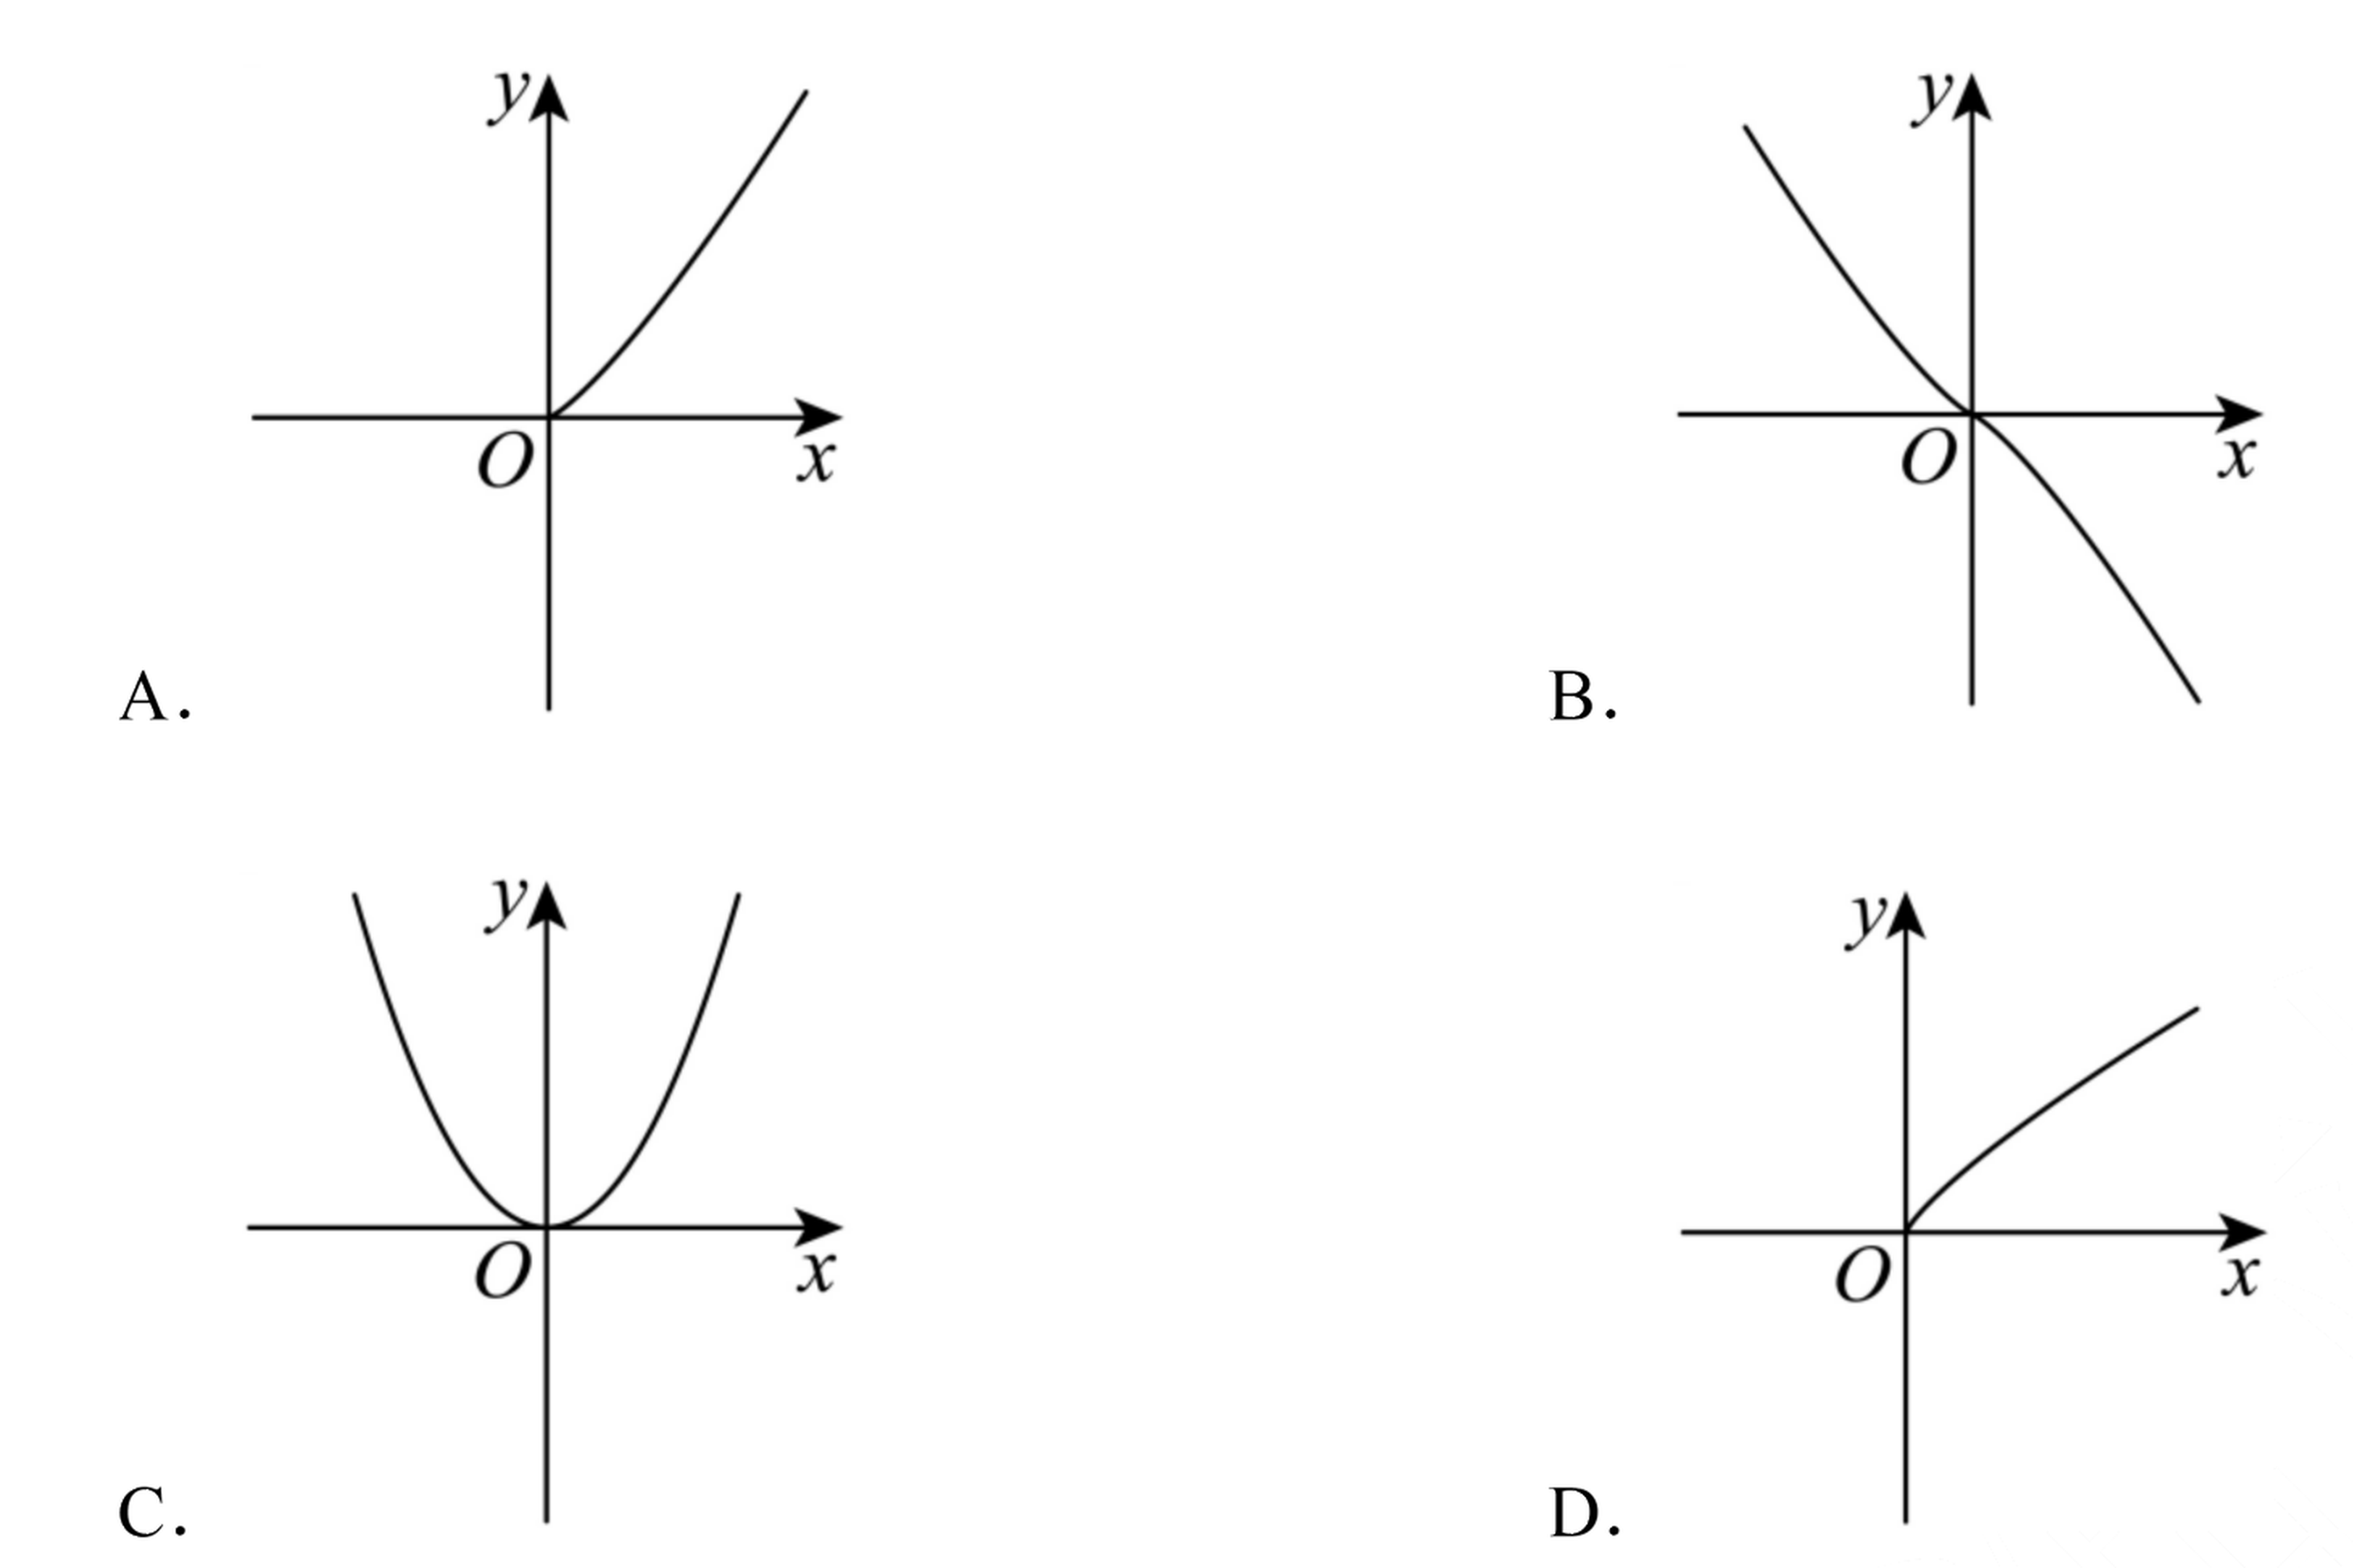
\includegraphics[width=0.80\textwidth]{figures/gao136_q13.png}
\end{center}

\ifanswer
\solbegin
\step{由 $y=x^{\frac54}=\sqrt[4]{x^5}$，函数的定义域为 $[0,+\infty)$，排除 BC，}% 原卷"排除 BC"连写，照录
\step{因为 $\dfrac54>1$，所以函数 $y=x^{\frac54}$ 的图象呈现下凸的趋势，排除 D. 故选 $A$.}
\solend
\fi

\item 下列不等式① $a+\dfrac1a\geqslant2$；② $a^2+4\geqslant4a$；③ $\left\lvert\dfrac ba+\dfrac ab\right\rvert\geqslant2$；④ $\dfrac{2a^2b^2}{a^2+b^2}\leqslant ab$；其中恒成立的是\mbox{（\quad）}

\keepwithprev
A. ①④\qquad B. ③④\qquad C. ②③\qquad D. ①②

\ifanswer
\ans{$C$}
\fi

\item 函数 $y=a^x+b-1(a>0,a\neq1)$ 单调递增且图象不经过第四象限，则 $a,b$ 满足的条件为\mbox{（\quad）}

\keepwithprev
A. $a>1,b\leqslant1$\qquad B. $a>1,b\geqslant0$\qquad C. $0<a<1,b\leqslant1$\qquad D. $0<a<1,b\geqslant1$

\ifanswer
\solbegin
\step{因为函数 $y=a^x+b-1$ 单调递增，所以 $a>1$，}
\step{图象不经过第四象限，则 $x=0$ 时，$y=b\geqslant0$，所以 $a>1,b\geqslant0$，故选 $B$.}
\solend
\fi

\item 设关于 $x$ 的不等式 $\dfrac{ax-1}{x^2-a}<0$ 的解集为 $S$，且 $3\in S$，$4\notin S$，则实数 $a$ 的取值范围为\mbox{（\quad）}

\keepwithprev
A. $(-\infty,-\sqrt3)\cup\left(\dfrac13,\sqrt3\right)$\qquad B. $\left(-\infty,\dfrac14\right)\cup(16,+\infty)$

C. $\left[\dfrac14,\dfrac13\right)\cup(9,16]$\qquad D. 不能确定

\ifanswer
\solbegin
\step{若 $3\in S$，则 $\dfrac{3a-1}{9-a}<0$，解得 $a\in\left(-\infty,\dfrac13\right)\cup(9,+\infty)$，}
\step{若 $4\notin S$，则 $16-a=0$ 或 $\dfrac{4a-1}{16-a}\geqslant0$，解得 $a\in\left[\dfrac14,16\right]$，}
\step{故实数 $a$ 的取值范围为 $\left[\dfrac14,\dfrac13\right)\cup(9,16]$，故选 $C$.}
\solend
\fi

\end{enumerate}

\bigsec{三、解答题}

\begin{enumerate}
\setcounter{enumi}{16}

\item 计算：(1) 计算 $\dfrac{\lg8+\lg125-\lg2-\lg5}{\lg\sqrt{10}\cdot\lg0.1}$；(2) 若 $a^{2x}=2(a>0)$，求 $\dfrac{a^{3x}+a^{-3x}}{a^x+a^{-x}}$.

\ifanswer
\solbegin
\step{(1) 原式 $=\dfrac{2-1}{\frac12\cdot(-1)}=-2$；(2) 原式 $=a^{2x}-1+a^{-2x}=2-1+\dfrac12=\dfrac32$.}
\solend
\fi

\item 不等式 $\dfrac{x-1}{x+1}\geqslant0$ 的解集为 $A$，不等式 $(x-a-1)(2a-x)>0(a<1)$ 的解集为 $B$.

(1) 求集合 $A$；

(2) 若 $B\subseteq A$，求实数 $a$ 的取值范围.

\ifanswer
\solbegin
\step{(1) $A=(-\infty,-1)\cup[1,+\infty)$.}
\step{(2) 由 $(x-a-1)(2a-x)>0(a<1)$，得 $(x-a-1)(x-2a)<0(a<1)$，}
\step{因为 $a<1$，所以 $a+1>2a$，所以 $B=(2a,a+1)$，}
\step{因为 $B\subseteq A$，所以 $2a\geqslant1$ 或 $a+1\leqslant-1$，即 $a\geqslant\dfrac12$ 或 $a\leqslant-2$，}
\step{而 $a<1$，所以实数 $a$ 的取值范围 $(-\infty,-2]\cup\left[\dfrac12,1\right)$.}% 原卷"取值范围"后脱"是／为"，照录
\solend
\fi

\item 已知幂函数 $y=x^m(m\in\R)$ 经过点 $\left(4,\dfrac12\right)$.

(1) 求此幂函数的表达式和定义域；

(2) 已知点 $A(a+2,y_1)$，点 $B(3-2a,y_2)(a\in\R)$ 在此幂函数的图像上，且满足 $y_1<y_2$，求实数 $a$ 的取值范围.

\ifanswer
\solbegin
\step{(1) 幂函数 $y=x^m(m\in\R)$ 经过点 $\left(4,\dfrac12\right)$，所以 $4^m=\dfrac12\Rightarrow m=-\dfrac12$，}
\step{所以 $f(x)=x^{-\frac12}$，定义域为 $(0,+\infty)$.}
\step{(2) 由于函数 $f(x)$ 在其定义域 $(0,+\infty)$ 上严格减，}
\step{由 $y_1<y_2$，得 $a+2>3-2a\geqslant0\Rightarrow a\in\left(\dfrac13,\dfrac32\right]$.}
\solend
\fi

% 第 20 题图取 05 页截图（0.42\textwidth、高约 6cm）。试排 \item 前加 7cm 守卫会多出
% 一张只有两行正文的稀疏页，且三版不加守卫时图均与题干、【解析】同页，故不另加守卫
\item 某医药研究所开发一种抗甲流新药，如果成年人按规定的剂量服用，据监测：服药后每毫升血液中的含药量 $y$（微克）与时间 $t$（小时）之间近似满足如图所示的曲线.

(1) 结合图，求 $k$ 与 $a$ 的值；

(2) 写出服药后 $y$ 与 $t$ 之间的函数关系式 $y=f(t)$；

(3) 据进一步测定：每毫升血液中含药量不少于 $0.5$ 微克时治疗疾病有效，求服药一次治疗有效的时间范围？

\begin{center}
% 图取原卷 05 页截图去粉色水印、去色，3x LANCZOS 放大
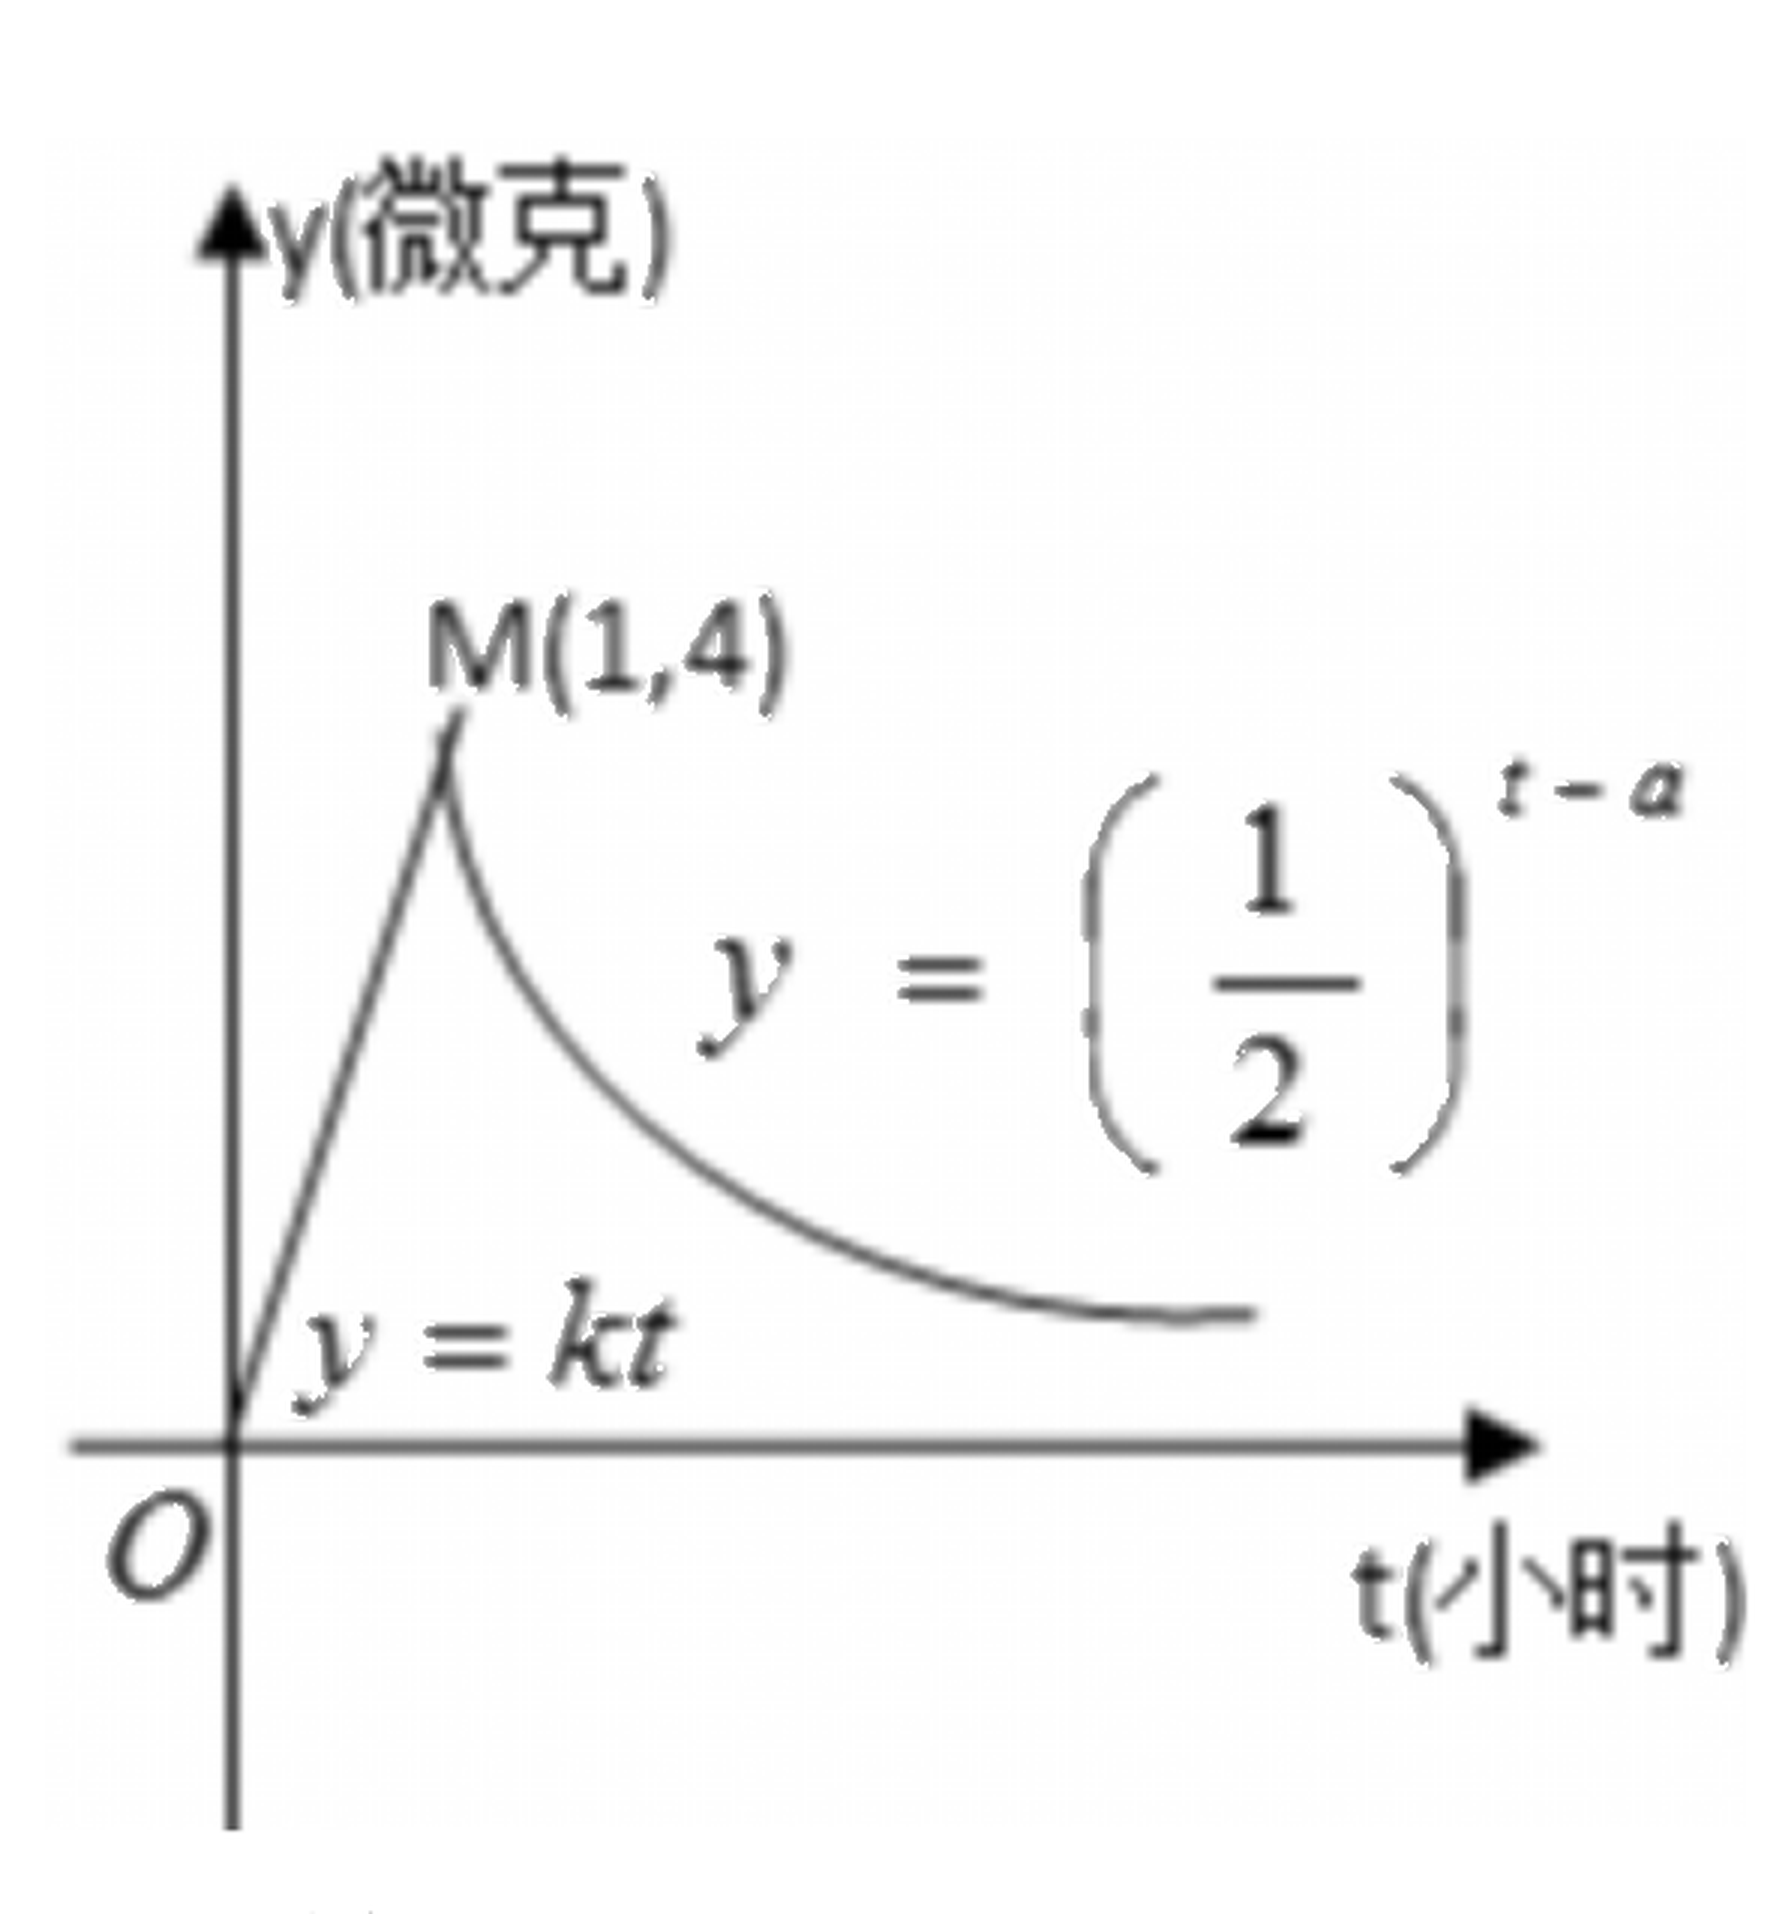
\includegraphics[width=0.42\textwidth]{figures/gao136_q20.png}
\end{center}

\ifanswer
\solbegin
\step{(1) 当 $0\leqslant t\leqslant1$ 时，函数图象是一条线段，由于过原点与点 $(1,4)$，所以 $k=4$，}
\step{其解析式为 $y=4t$，$0\leqslant t\leqslant1$；}
\step{当 $t\geqslant1$ 时，函数的解析式为 $y=\left(\dfrac12\right)^{t-a}$，}
\step{此时 $M(1,4)$ 在曲线上，将此点的坐标代入函数解析式得 $4=\left(\dfrac12\right)^{1-a}$，}
\step{解得 $a=3$；}
\step{(2) 由 (1) 得 $f(t)=\begin{cases}4t,0\leqslant t\leqslant1\\\left(\frac12\right)^{t-3},t>1\end{cases}$；}
\step{(3) 由 (2) 得，令 $f(t)\geqslant0.5$，即 $\begin{cases}4t\geqslant0.5,0\leqslant t\leqslant1\\\left(\frac12\right)^{t-3}\geqslant0.5,t>1\end{cases}$，所以 $\dfrac18\leqslant t\leqslant4$.}
\solend
\fi

\item 已知关于 $x$ 的不等式 $(kx-k^2-4)(x-4)>0$，其中 $k\in\R$.

(1) 当 $k=-1$，求不等式的解集 $A$；

(2) 当 $k$ 变化时，试求不等式的解集 $A$；

(3) 对于不等式解集 $A$，满足 $A\cap\Z=B$. 试探究集合 $B$ 能否为有限集，若能，求出使得集合 $B$ 中元素最少的 $k$ 的所有取值，并用列举法表示此时的集合 $B$，若不能，说明理由；

\ifanswer
\solbegin
\step{(1) 当 $k=-1$ 时，原不等式可化为 $(x+5)(x-4)<0$，}
\step{解得 $-5<x<4$，故不等式的解集为 $\{x\mid -5<x<4\}$；}
\step{(2) 当 $k=0$ 时，解集为 $\{x\mid x<4\}$，}
\step{当 $k>0$ 时，$\dfrac{k^2+4}{k}=k+\dfrac4k\geqslant4$，解集为 $\{x\mid x<4\text{ 或 }x>\dfrac{k^2+4}{k}\}$；}
\step{当 $k<0$ 时，解集为 $\{x\mid \dfrac{k^2+4}{k}<x<4\}$，}
\step{综上，当 $k=0$ 时，$A=\{x\mid x<4\}$，}
\step{当 $k>0$ 时，$A=\{x\mid x<4\text{ 或 }x>\dfrac{k^2+4}{k}\}$；}
\step{当 $k<0$ 时，$A=\{x\mid \dfrac{k^2+4}{k}<x<4\}$，}
\step{(3) 由 (2) 得当 $k\geqslant0$ 时，$B$ 为无限集，当 $k<0$ 时，$B$ 为有限集，}
\step{此时，$\dfrac{k^2+4}{k}=k+\dfrac4k\leqslant-4$，当且仅当 $k=-2$ 时取等号，}
\step{所以 $k=-2$ 时，$B$ 中元素最少，此时 $A=\{x\mid -4<x<4\}$，}
\step{所以 $B=\{-3,-2,-1,0,1,2,3\}$.}
\solend
\fi

\end{enumerate}

% 第 22 题是"四、附加题"首题且带 9cm 图块，守卫须放在 \bigsec 之前连节标题一起量，
% 否则"四、附加题"会孤立在页末（B 类，照 高一26／40／59 成例）
\needvspace{11cm}
\bigsec{四、附加题}

\begin{enumerate}
\setcounter{enumi}{21}

% 第 22 题四幅抛物线/坐标图选项是一整块，守卫放在 \item 之前
\needvspace{9cm}
\item 函数 $f(x)=\left(\dfrac12\right)^{\lvert x+1\rvert}$ 的图象大致为\mbox{（\quad）}

\keepwithprev
\begin{center}
% 四幅抛物线/坐标图选项取原卷 07 页截图去粉色水印，按原卷 2x2 排布合并为一张
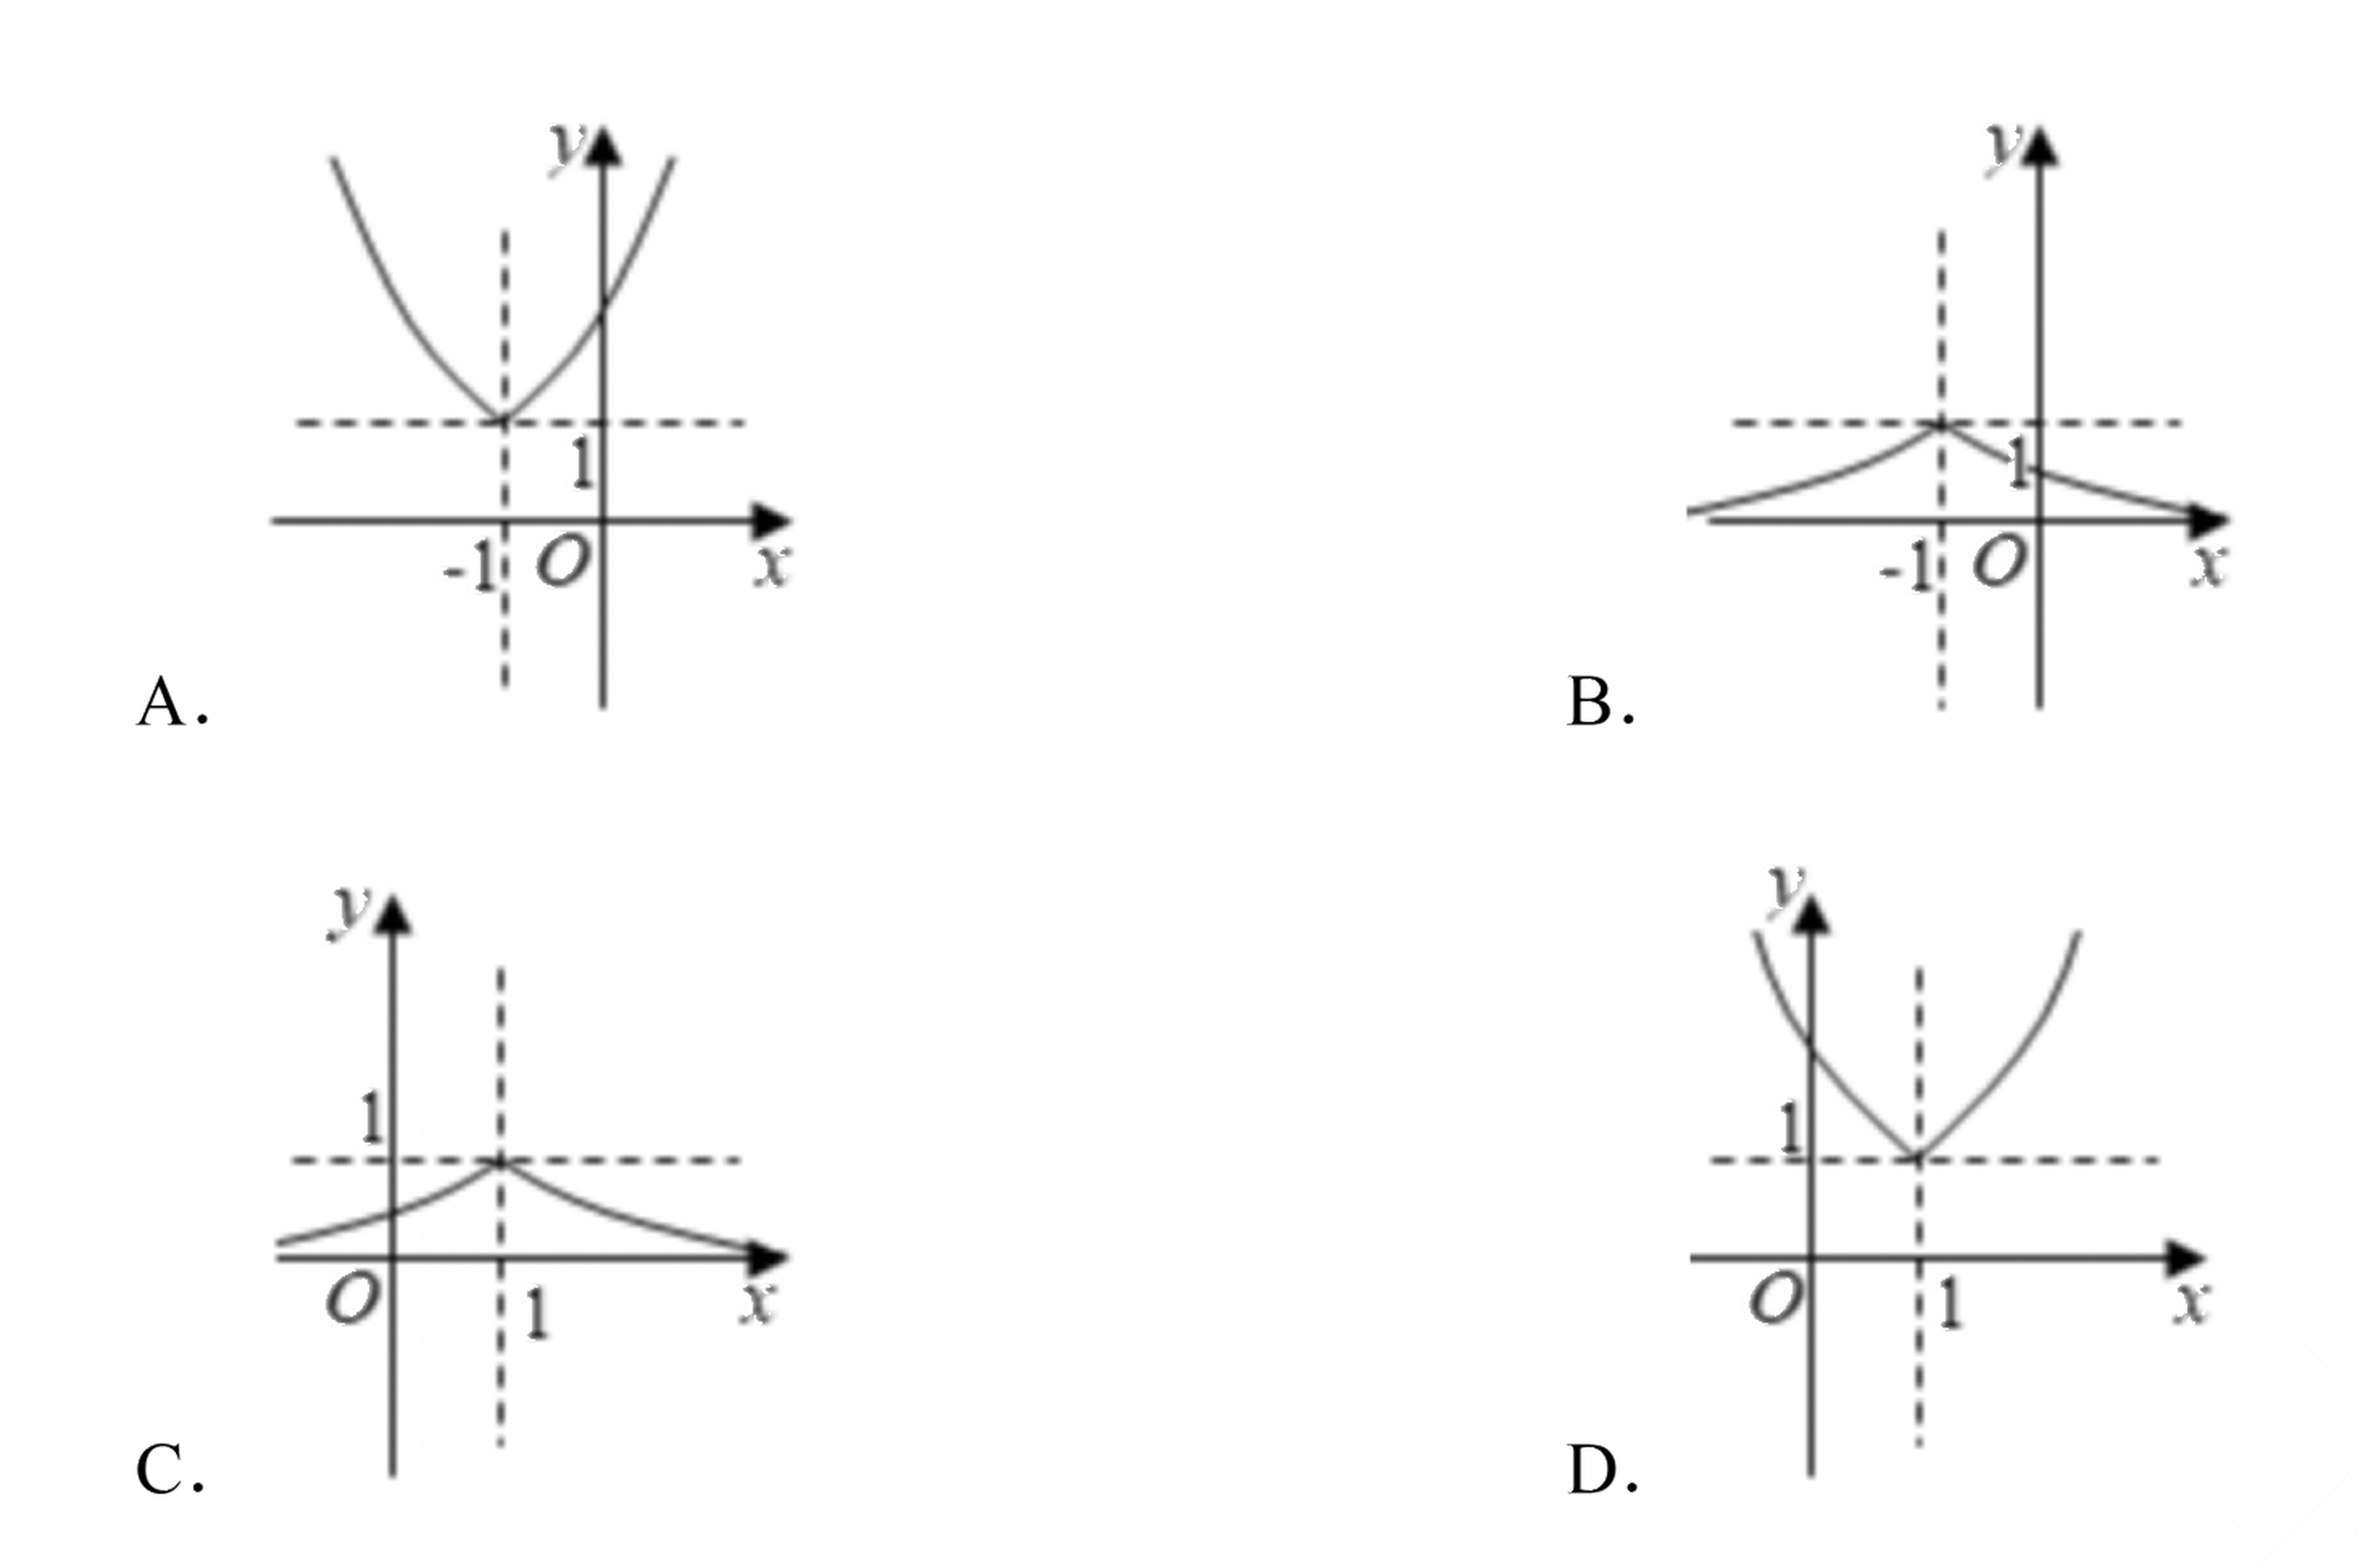
\includegraphics[width=0.80\textwidth]{figures/gao136_q22.png}
\end{center}

\ifanswer
\ans{$B$}
\fi

\end{enumerate}

\end{document}
"
%
% ① 原始材料：微信公众号"魔都数学加油站"文章，作者破晓，2026-11-15 18:04 发布；
% 连载"27学年高一136"，原文标题"27学年高一136——2026-2027年上海市三林中学高一上期中"；
% 原文链接：https://mp.weixin.qq.com/s/jaMzqMm6pDvcT0yM0d7eaQ。
% 正文为 7 张 PNG 页（01、04、06 为 4762x6735；02、03、05、07 为 2560x3620，
% 同一篇各页分辨率不同，逐页按各自分辨率裁图核对），题目下印有【答案】或【解析】，为讲评版。
% 题目、解析均据原图转录；卷面粉红色水印"魔都数学加油站"及公众号页脚未录入。
% 全卷 3 幅插图：第 13 题四幅坐标图选项（03 页）、第 20 题药物浓度折线/曲线图（05 页）、
% 第 22 题四幅抛物线/坐标图选项（07 页），均取原卷截图去粉色水印、去色、LANCZOS 放大，
% 四幅选项按原卷 2x2 排布合并为一张；图前按惯例加 \needvspace 守卫。
%
% 卷首标题：原卷印作"2026-2027 年三林中学高一上期中"（公众号标题中的"上海市"
% 卷面标题行没有，本稿照卷面），年份区间按全稿惯例排 en dash；原卷未印副标题，
% 本卷为期中卷、跨集合与常用逻辑用语／不等式／函数三章，按题目内容标为
% "集合与常用逻辑用语、不等式、函数"（与 125／126／128／129／131／132／133 同期中卷口径相同）：
% 集合与逻辑见 Q3、Q6、Q10、Q12、Q16、Q18、Q21，不等式见 Q5、Q7、Q8、Q9、Q14、Q15，
% 函数（幂函数、指数／对数、基本不等式应用）见 Q4、Q11、Q13、Q17、Q19、Q20、Q22。
%
% 题号体例：本卷共 20 题——一、填空题 3—12（10 题）、二、选择题 13—16（4 题）、
% 三、解答题 17—21（5 题）、四、附加题 22（1 题）。四节分别
% \setcounter{enumi}{2}／{12}／{16}／{21}。
%
% ② 与原卷的排版差异：
%   ① 原文从第 3 题起，本稿保留原题号；末节"四、附加题"另起 \bigsec，题号续到 22；
%   ② 原卷每题下直接印【答案】或【解析】，本稿按全稿惯例置于答案版；第 3、4、6 题只印
%      【答案】、无【解析】，提 \ans{}；第 14 题答案 C 印在题干括号内、无【解析】，按
%      高一53／高一108／高一132／高一133 成例括号留空、另提 \ans{$C$}；第 22 题答案 B
%      印在题干括号内、无【解析】，同例提 \ans{$B$}；第 13、15、16 题答案在解析末句
%      "故选 …"，括号内留空、不另提 \ans{}；其余各题印【解析】、无独立答案段；
%   ③ 原卷未印副标题，本稿按"知识模块"口径补出；
%   ④ 原卷填空横线按全稿惯例排为 \blankline[4.4em]；选择题括号排 \mbox{（\quad）}、
%      每个选项段前按惯例加 \keepwithprev（四幅图选项那一枚放在 \begin{center} 之前）；
%      解答题不留作答区、不加 \anspace（原卷为讲评版，与 129／131／132／133 同）；
%   ⑤ 原卷数集排斜体 $R$／$R^+$／$Z$，按全稿惯例改 \R／\R^+／\Z；空集记号 \varnothing；
%      绝对值排 \lvert…\rvert，集合描述竖线排 \mid；不等号按全稿惯例排 \leqslant／\geqslant；
%   ⑥ 子题标号 (1)(2)(3) 原卷用半角括号，照录；圈数字 ①②③④ 照录；第 12 题甲／乙／丙
%      三行与第 14 题四个编号不等式照录；
%   ⑦ 数学式内半角逗号照录（如 Q4"$a>0,a\neq1$"、Q6"$\{(-2,4),(1,1)\}$"、
%      Q7"$a=2+3=5,b=2\times3=6$"、Q11"$x_1,x_2$"、Q12"$m,n\in R^+$"、
%      Q15"$a>1,b\geq0$"、Q18"$B=(2a,a+1)$"、Q20"$4t,0\leq t\leq1$"、
%      Q21"$\{-3,-2,-1,0,1,2,3\}$"）；原卷行末西文句点照录，行中全角逗号照录；
%   ⑧ 三幅插图：第 13 题四幅坐标图选项合并裁为一张 \includegraphics（题前 \needvspace{9cm}）；
%      第 20 题折线/曲线图取 05 页截图（0.42\textwidth）；第 22 题四幅抛物线/坐标图选项合并
%      裁为一张（题前 \needvspace{9cm}）。第 13、22 题分别是"二、选择题""四、附加题"的首题
%      且带大图块，另在两处 \bigsec 之前各加 \needvspace{11cm} 连节标题一起量，避免节标题
%      孤立在页末（切页审计 B 类；照 高一26／40／59 成例）。第 20 题图不是节首题、三版试排
%      图均与题干同页，加 7cm 守卫反会多出一张只有两行正文的稀疏页，故不另加守卫；
%      三版切页审计均"合计异常：无"（试卷 4 页／紧凑 4 页／答案 6 页）；
%   ⑨ 跨页续印按题合并：Q16 题干在 03 页、括号与选项及【解析】在 04 页；Q19 题干在 04 页、
%      (2) 与【解析】在 05 页；Q20 (3)【解析】在 06 页；Q22 四幅图在 07 页；本稿按题连排；
%   ⑩ 题干中的中文弯引号按原卷照录，注释内一律 ASCII 引号；原卷"图像／图象"两种写法混用，
%      逐处照录（Q4、Q19 作"图像"，Q13、Q15、Q20、Q22 作"图象"）；
%   ⑪ 附加题节：原卷印"四、附加题"，本稿用 \bigsec{四、附加题} 另起一节、
%      \setcounter{enumi}{21}，顶层 1 个 \item（与 高一09／15／16／22／35／39／47／61 同口径）；
%      Q22 只印括号内答案、提 \ans{}，不计入 \step 账。
%
% 判别式字形：全卷仅第 9 题【解析】cases 块出现判别式"$\Delta=a^2-8a<0$"，原卷印
%   等腰、偏高的三角 $\Delta$，逐处放大核对并照录 \Delta；全卷未出现扁等边三角 \triangle。
%
% 子集符号：第 18 题 (2) 题干"$B\subseteq A$"与【解析】"$B\subseteq A$"两处原卷均印
%   带下划线 $\subseteq$，逐处放大核对、照录 \subseteq；全卷未出现单线 \subset。
%
% 原卷存疑照录（均照录未改，正文对应处另有 % 注）：
%   第 12 题乙行"$\dfrac{m+n}{mm}=\dfrac1{mn}$"前一分母印作 $mm$（后一处作 $mn$），照录；
%   第 12 题【解析】"$\geqslant\dfrac1{100}\left[a^2+1+2\sqrt{a^2}\right]$"保留 $\sqrt{a^2}$
%      未化简为 $a$，照录；
%   第 13 题【解析】"排除 BC"与"排除 D"连写选项字母，照录；
%   第 18 题 (2)【解析】末行"所以实数 $a$ 的取值范围 $(-\infty,-2]\cup[\frac12,1)$"
%      "取值范围"后脱"是／为"字，照录；
%   第 21 题 (3) 题干"求出使得集合 $B$ 中元素最少的 $k$ 的所有取值"而【解析】只给出
%      $k=-2$ 一处，措辞照录。
%
% 行数复核：逐题数 \step 条数，合计 51 条（Q3：0；Q4：0；Q5：2；Q6：0；Q7：2；Q8：1；
% Q9：1；Q10：4；Q11：1；Q12：4；Q13：2；Q14：0；Q15：2；Q16：3；Q17：1；Q18：5；
% Q19：4；Q20：7；Q21：12；Q22：0），与原卷印刷行逐题相等（cases 块作一个印刷行计）。
% 第 3、4、6、14、22 题只印【答案】、提 \ans{}，不计入 \step 账；第 13、15、16 题答案在
% 解析末句，括号内留空、不另提 \ans{}。
%
\documentclass[a4paper,11pt]{article}
\usepackage{common}

\begin{document}

\examtitlest[3]{2026--2027 年三林中学高一上期中}{集合与常用逻辑用语、不等式、函数}

\bigsec{一、填空题}

\begin{enumerate}
\setcounter{enumi}{2}

\item 用反证法证明命题“若 $x+y\neq5$，则 $x\neq2$ 或 $y\neq3$”为真命题时，第一个步骤是\blankline[4.4em].

\ifanswer
\ans{假设 $x=2$ 且 $y=3$}
\fi

\item 函数 $y=a^{x-1}+1(a>0,a\neq1)$ 的图像恒过定点 $A$，则点的坐标是\blankline[4.4em].

\ifanswer
\ans{$(1,2)$}
\fi

\item 已知 $x>1$，则 $x+\dfrac4{x-1}$ 的最小值是\blankline[4.4em].

\ifanswer
\solbegin
\step{由 $x>1$，得 $x-1>0$，则 $x+\dfrac4{x-1}=x-1+\dfrac4{x-1}+1\geqslant2\sqrt{(x-1)\cdot\dfrac4{x-1}}+1=5$，}
\step{当且仅当 $x-1=\dfrac4{x-1}$ 即 $x=3$ 时取等号，取得最小值 $5$.}
\solend
\fi

\item 已知集合 $A=\{(x,y)\mid y=x^2\}$，集合 $B=\{(x,y)\mid y=2-x\}$，求 $A\cap B=$\blankline[4.4em].

\ifanswer
\ans{$\{(-2,4),(1,1)\}$}
\fi

\item 已知一元二次不等式 $x^2-ax+b<0$ 的解集为 $(2,3)$，则不等式 $bx^2-ax+1>0$ 的解集是\blankline[4.4em].

\ifanswer
\solbegin
\step{$a=2+3=5,b=2\times3=6$，则 $bx^2-ax+1>0$ 即 $6x^2-5x+1>0$，}
\step{即 $(3x-1)(2x-1)>0$，解集为 $\left(-\infty,\dfrac13\right)\cup\left(\dfrac12,+\infty\right)$.}
\solend
\fi

\item 不等式 $(x+2)^3<(5-2x)^3$ 的解集为\blankline[4.4em].

\ifanswer
\solbegin
\step{由 $(x+2)^3<(5-2x)^3$ 得 $x+2<5-2x$，故解集为 $(-\infty,1)$.}
\solend
\fi

\item 若关于 $x$ 的不等式 $ax^2-ax+2>0$ 的解集为 $\R$，则实数 $a$ 的取值范围是\blankline[4.4em].

\ifanswer
\solbegin
\step{由题意得 $a=0$ 或 $\begin{cases}a>0\\\Delta=a^2-8a<0\end{cases}$，所以 $0\leqslant a<8$.}% 判别式原卷印高三角 $\Delta$，照录
\solend
\fi

\item 已知关于 $x$ 的不等式 $\lvert x+3\rvert+\lvert x-a\rvert\geqslant5$ 恒成立，则实数 $a$ 的取值范围为\blankline[4.4em].

\ifanswer
\solbegin
\step{因为 $\lvert x+3\rvert+\lvert x-a\rvert\geqslant\lvert x-a-x-3\rvert=\lvert 3+a\rvert$，}
\step{要使 $\lvert x+3\rvert+\lvert x-a\rvert\geqslant5$ 恒成立，则 $\lvert a+3\rvert\geqslant5$ 即可，}
\step{所以 $a+3\geqslant5$ 或 $a+3\leqslant-5$，解得 $a\geqslant2$ 或 $a\leqslant-8$，}
\step{即实数 $a$ 的取值范围是 $(-\infty,-8]\cup[2,+\infty)$.}
\solend
\fi

\item 若方程 $\lg^2 x-2\lg x-2=0$ 的两个解为 $x_1,x_2$，求 $\log_{x_1}x_2+\log_{x_2}x_1$ 的值为\blankline[4.4em].

\ifanswer
\solbegin
\step{$\log_{x_1}x_2+\log_{x_2}x_1=\dfrac{\lg x_2}{\lg x_1}+\dfrac{\lg x_1}{\lg x_2}=\dfrac{(\lg x_1+\lg x_2)^2-2\lg x_1\lg x_2}{\lg x_1\lg x_2}=-4$.}
\solend
\fi

\item 三个同学对问题“已知 $m,n\in \R^+$，且 $m+n=1$，求 $\dfrac1m+\dfrac1n$ 的最小值”提出各自的解题思路：

思路：

甲：$\dfrac1m+\dfrac1n=\dfrac{m+n}{m}+\dfrac{m+n}{n}=2+\dfrac nm+\dfrac mn$，可用基本不等式求解；

乙：$\dfrac1m+\dfrac1n=\dfrac{m+n}{mm}=\dfrac1{mn}=\dfrac1{m(1-m)}$，可用二次函数配方法求解；% 原卷前一分母印作 $mm$，照录

丙：$\dfrac1m+\dfrac1n=\left(\dfrac1m+\dfrac1n\right)(m+n)=2+\dfrac nm+\dfrac mn$，可用基本不等式求解；参考上述解题思路，

可求得当 $x=$\blankline[4.4em]时，$y=\dfrac{a^2}{x^2}+\dfrac1{100-x^2}$（$0<x<10$，$a>0$）有最小值.

\ifanswer
\solbegin
\step{$y=\dfrac{a^2}{x^2}+\dfrac1{100-x^2}=\left(\dfrac{a^2}{x^2}+\dfrac1{100-x^2}\right)[x^2+(100-x^2)]\times\dfrac1{100}$}
\step{$=\dfrac1{100}\left[a^2+1+\dfrac{x^2}{100-x^2}+\dfrac{a^2(100-x^2)}{x^2}\right]\geqslant\dfrac1{100}\left[a^2+1+2\sqrt{a^2}\right]$}% 原卷保留 $\sqrt{a^2}$ 未化简，照录
\step{当且仅当 $\dfrac{x^2}{100-x^2}=\dfrac{a^2(100-x^2)}{x^2}$，即 $x=\sqrt{\dfrac{100a}{a+1}}$ 时，}
\step{$y=\dfrac{a^2}{x^2}+\dfrac1{100-x^2}(0<x<10,a>0)$ 有最小值.}
\solend
\fi

\end{enumerate}

% 第 13 题是"二、选择题"首题且带 9cm 图块，守卫须放在 \bigsec 之前连节标题一起量，
% 否则"二、选择题"会孤立在页末（B 类，照 高一26／40／59 成例）
\needvspace{11cm}
\bigsec{二、选择题}

\begin{enumerate}
\setcounter{enumi}{12}

% 第 13 题四幅坐标图选项是一整块，守卫放在 \item 之前
\needvspace{9cm}
\item 下列图象中，最符合函数 $y=x^{\frac54}$ 的图象的是\mbox{（\quad）}

\keepwithprev
\begin{center}
% 四幅坐标图选项取原卷 03 页截图去粉色水印，按原卷 2x2 排布合并为一张
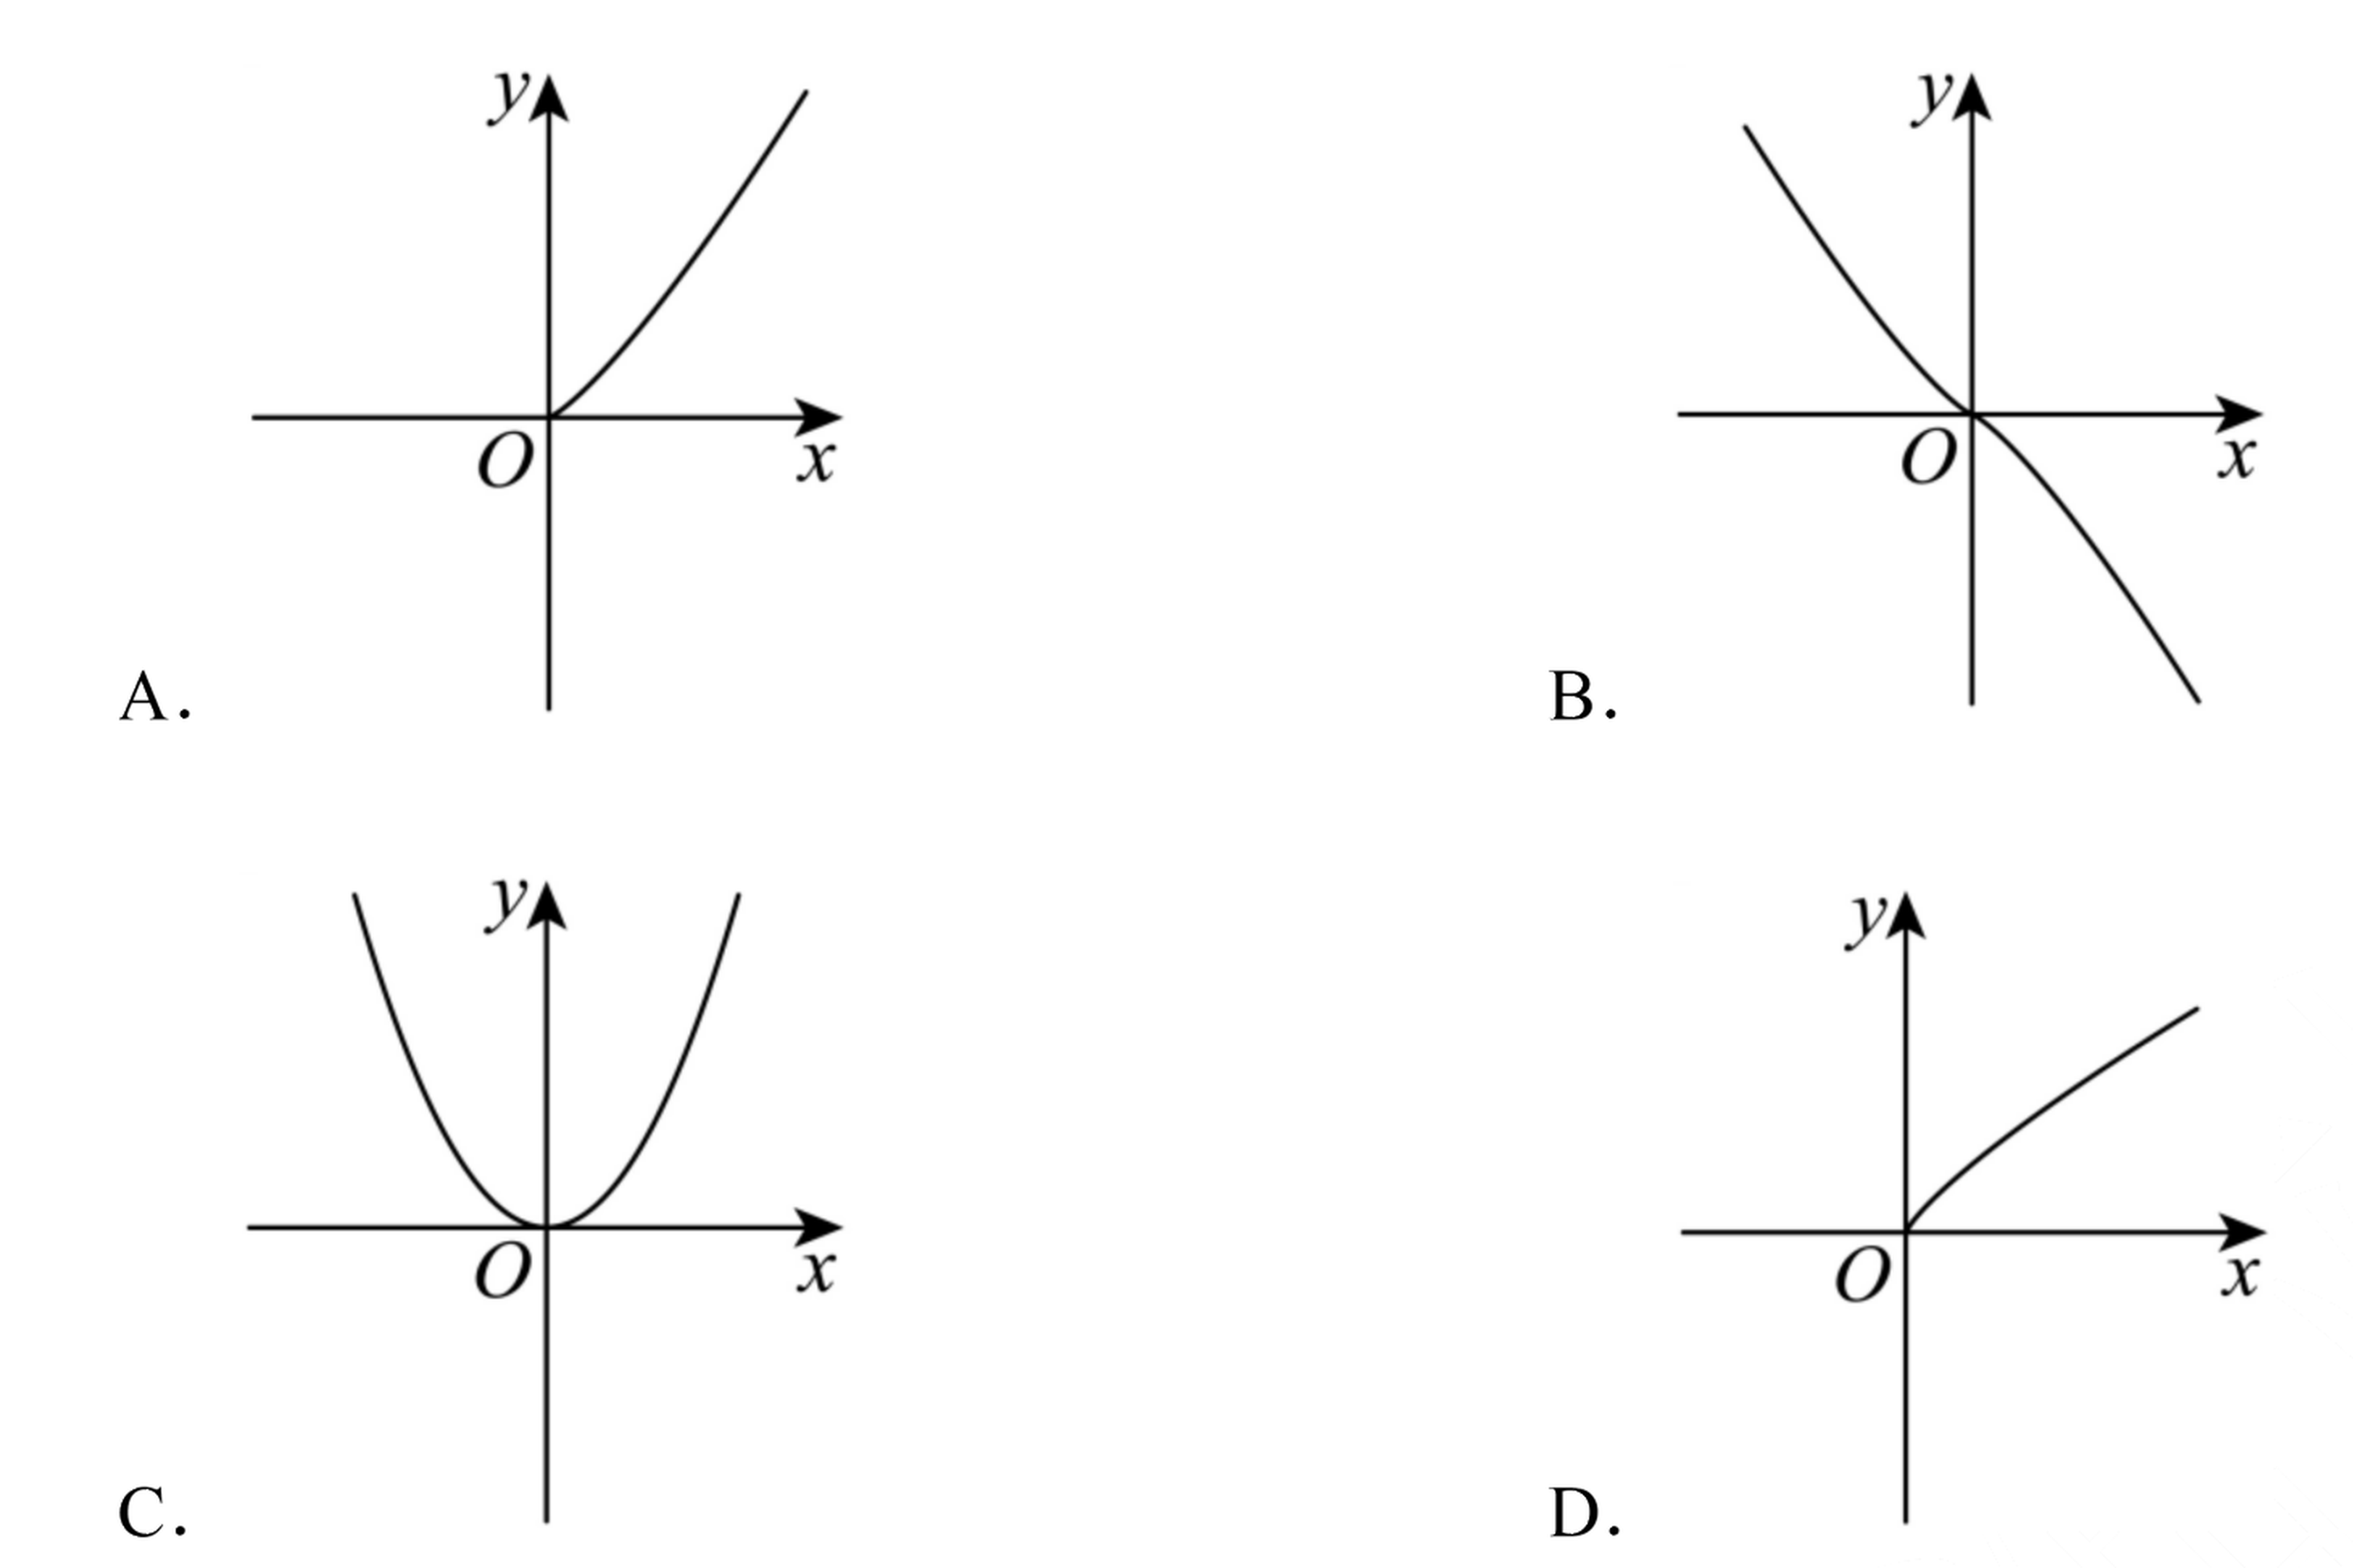
\includegraphics[width=0.80\textwidth]{figures/gao136_q13.png}
\end{center}

\ifanswer
\solbegin
\step{由 $y=x^{\frac54}=\sqrt[4]{x^5}$，函数的定义域为 $[0,+\infty)$，排除 BC，}% 原卷"排除 BC"连写，照录
\step{因为 $\dfrac54>1$，所以函数 $y=x^{\frac54}$ 的图象呈现下凸的趋势，排除 D. 故选 $A$.}
\solend
\fi

\item 下列不等式① $a+\dfrac1a\geqslant2$；② $a^2+4\geqslant4a$；③ $\left\lvert\dfrac ba+\dfrac ab\right\rvert\geqslant2$；④ $\dfrac{2a^2b^2}{a^2+b^2}\leqslant ab$；其中恒成立的是\mbox{（\quad）}

\keepwithprev
A. ①④\qquad B. ③④\qquad C. ②③\qquad D. ①②

\ifanswer
\ans{$C$}
\fi

\item 函数 $y=a^x+b-1(a>0,a\neq1)$ 单调递增且图象不经过第四象限，则 $a,b$ 满足的条件为\mbox{（\quad）}

\keepwithprev
A. $a>1,b\leqslant1$\qquad B. $a>1,b\geqslant0$\qquad C. $0<a<1,b\leqslant1$\qquad D. $0<a<1,b\geqslant1$

\ifanswer
\solbegin
\step{因为函数 $y=a^x+b-1$ 单调递增，所以 $a>1$，}
\step{图象不经过第四象限，则 $x=0$ 时，$y=b\geqslant0$，所以 $a>1,b\geqslant0$，故选 $B$.}
\solend
\fi

\item 设关于 $x$ 的不等式 $\dfrac{ax-1}{x^2-a}<0$ 的解集为 $S$，且 $3\in S$，$4\notin S$，则实数 $a$ 的取值范围为\mbox{（\quad）}

\keepwithprev
A. $(-\infty,-\sqrt3)\cup\left(\dfrac13,\sqrt3\right)$\qquad B. $\left(-\infty,\dfrac14\right)\cup(16,+\infty)$

C. $\left[\dfrac14,\dfrac13\right)\cup(9,16]$\qquad D. 不能确定

\ifanswer
\solbegin
\step{若 $3\in S$，则 $\dfrac{3a-1}{9-a}<0$，解得 $a\in\left(-\infty,\dfrac13\right)\cup(9,+\infty)$，}
\step{若 $4\notin S$，则 $16-a=0$ 或 $\dfrac{4a-1}{16-a}\geqslant0$，解得 $a\in\left[\dfrac14,16\right]$，}
\step{故实数 $a$ 的取值范围为 $\left[\dfrac14,\dfrac13\right)\cup(9,16]$，故选 $C$.}
\solend
\fi

\end{enumerate}

\bigsec{三、解答题}

\begin{enumerate}
\setcounter{enumi}{16}

\item 计算：(1) 计算 $\dfrac{\lg8+\lg125-\lg2-\lg5}{\lg\sqrt{10}\cdot\lg0.1}$；(2) 若 $a^{2x}=2(a>0)$，求 $\dfrac{a^{3x}+a^{-3x}}{a^x+a^{-x}}$.

\ifanswer
\solbegin
\step{(1) 原式 $=\dfrac{2-1}{\frac12\cdot(-1)}=-2$；(2) 原式 $=a^{2x}-1+a^{-2x}=2-1+\dfrac12=\dfrac32$.}
\solend
\fi

\item 不等式 $\dfrac{x-1}{x+1}\geqslant0$ 的解集为 $A$，不等式 $(x-a-1)(2a-x)>0(a<1)$ 的解集为 $B$.

(1) 求集合 $A$；

(2) 若 $B\subseteq A$，求实数 $a$ 的取值范围.

\ifanswer
\solbegin
\step{(1) $A=(-\infty,-1)\cup[1,+\infty)$.}
\step{(2) 由 $(x-a-1)(2a-x)>0(a<1)$，得 $(x-a-1)(x-2a)<0(a<1)$，}
\step{因为 $a<1$，所以 $a+1>2a$，所以 $B=(2a,a+1)$，}
\step{因为 $B\subseteq A$，所以 $2a\geqslant1$ 或 $a+1\leqslant-1$，即 $a\geqslant\dfrac12$ 或 $a\leqslant-2$，}
\step{而 $a<1$，所以实数 $a$ 的取值范围 $(-\infty,-2]\cup\left[\dfrac12,1\right)$.}% 原卷"取值范围"后脱"是／为"，照录
\solend
\fi

\item 已知幂函数 $y=x^m(m\in\R)$ 经过点 $\left(4,\dfrac12\right)$.

(1) 求此幂函数的表达式和定义域；

(2) 已知点 $A(a+2,y_1)$，点 $B(3-2a,y_2)(a\in\R)$ 在此幂函数的图像上，且满足 $y_1<y_2$，求实数 $a$ 的取值范围.

\ifanswer
\solbegin
\step{(1) 幂函数 $y=x^m(m\in\R)$ 经过点 $\left(4,\dfrac12\right)$，所以 $4^m=\dfrac12\Rightarrow m=-\dfrac12$，}
\step{所以 $f(x)=x^{-\frac12}$，定义域为 $(0,+\infty)$.}
\step{(2) 由于函数 $f(x)$ 在其定义域 $(0,+\infty)$ 上严格减，}
\step{由 $y_1<y_2$，得 $a+2>3-2a\geqslant0\Rightarrow a\in\left(\dfrac13,\dfrac32\right]$.}
\solend
\fi

% 第 20 题图取 05 页截图（0.42\textwidth、高约 6cm）。试排 \item 前加 7cm 守卫会多出
% 一张只有两行正文的稀疏页，且三版不加守卫时图均与题干、【解析】同页，故不另加守卫
\item 某医药研究所开发一种抗甲流新药，如果成年人按规定的剂量服用，据监测：服药后每毫升血液中的含药量 $y$（微克）与时间 $t$（小时）之间近似满足如图所示的曲线.

(1) 结合图，求 $k$ 与 $a$ 的值；

(2) 写出服药后 $y$ 与 $t$ 之间的函数关系式 $y=f(t)$；

(3) 据进一步测定：每毫升血液中含药量不少于 $0.5$ 微克时治疗疾病有效，求服药一次治疗有效的时间范围？

\begin{center}
% 图取原卷 05 页截图去粉色水印、去色，3x LANCZOS 放大
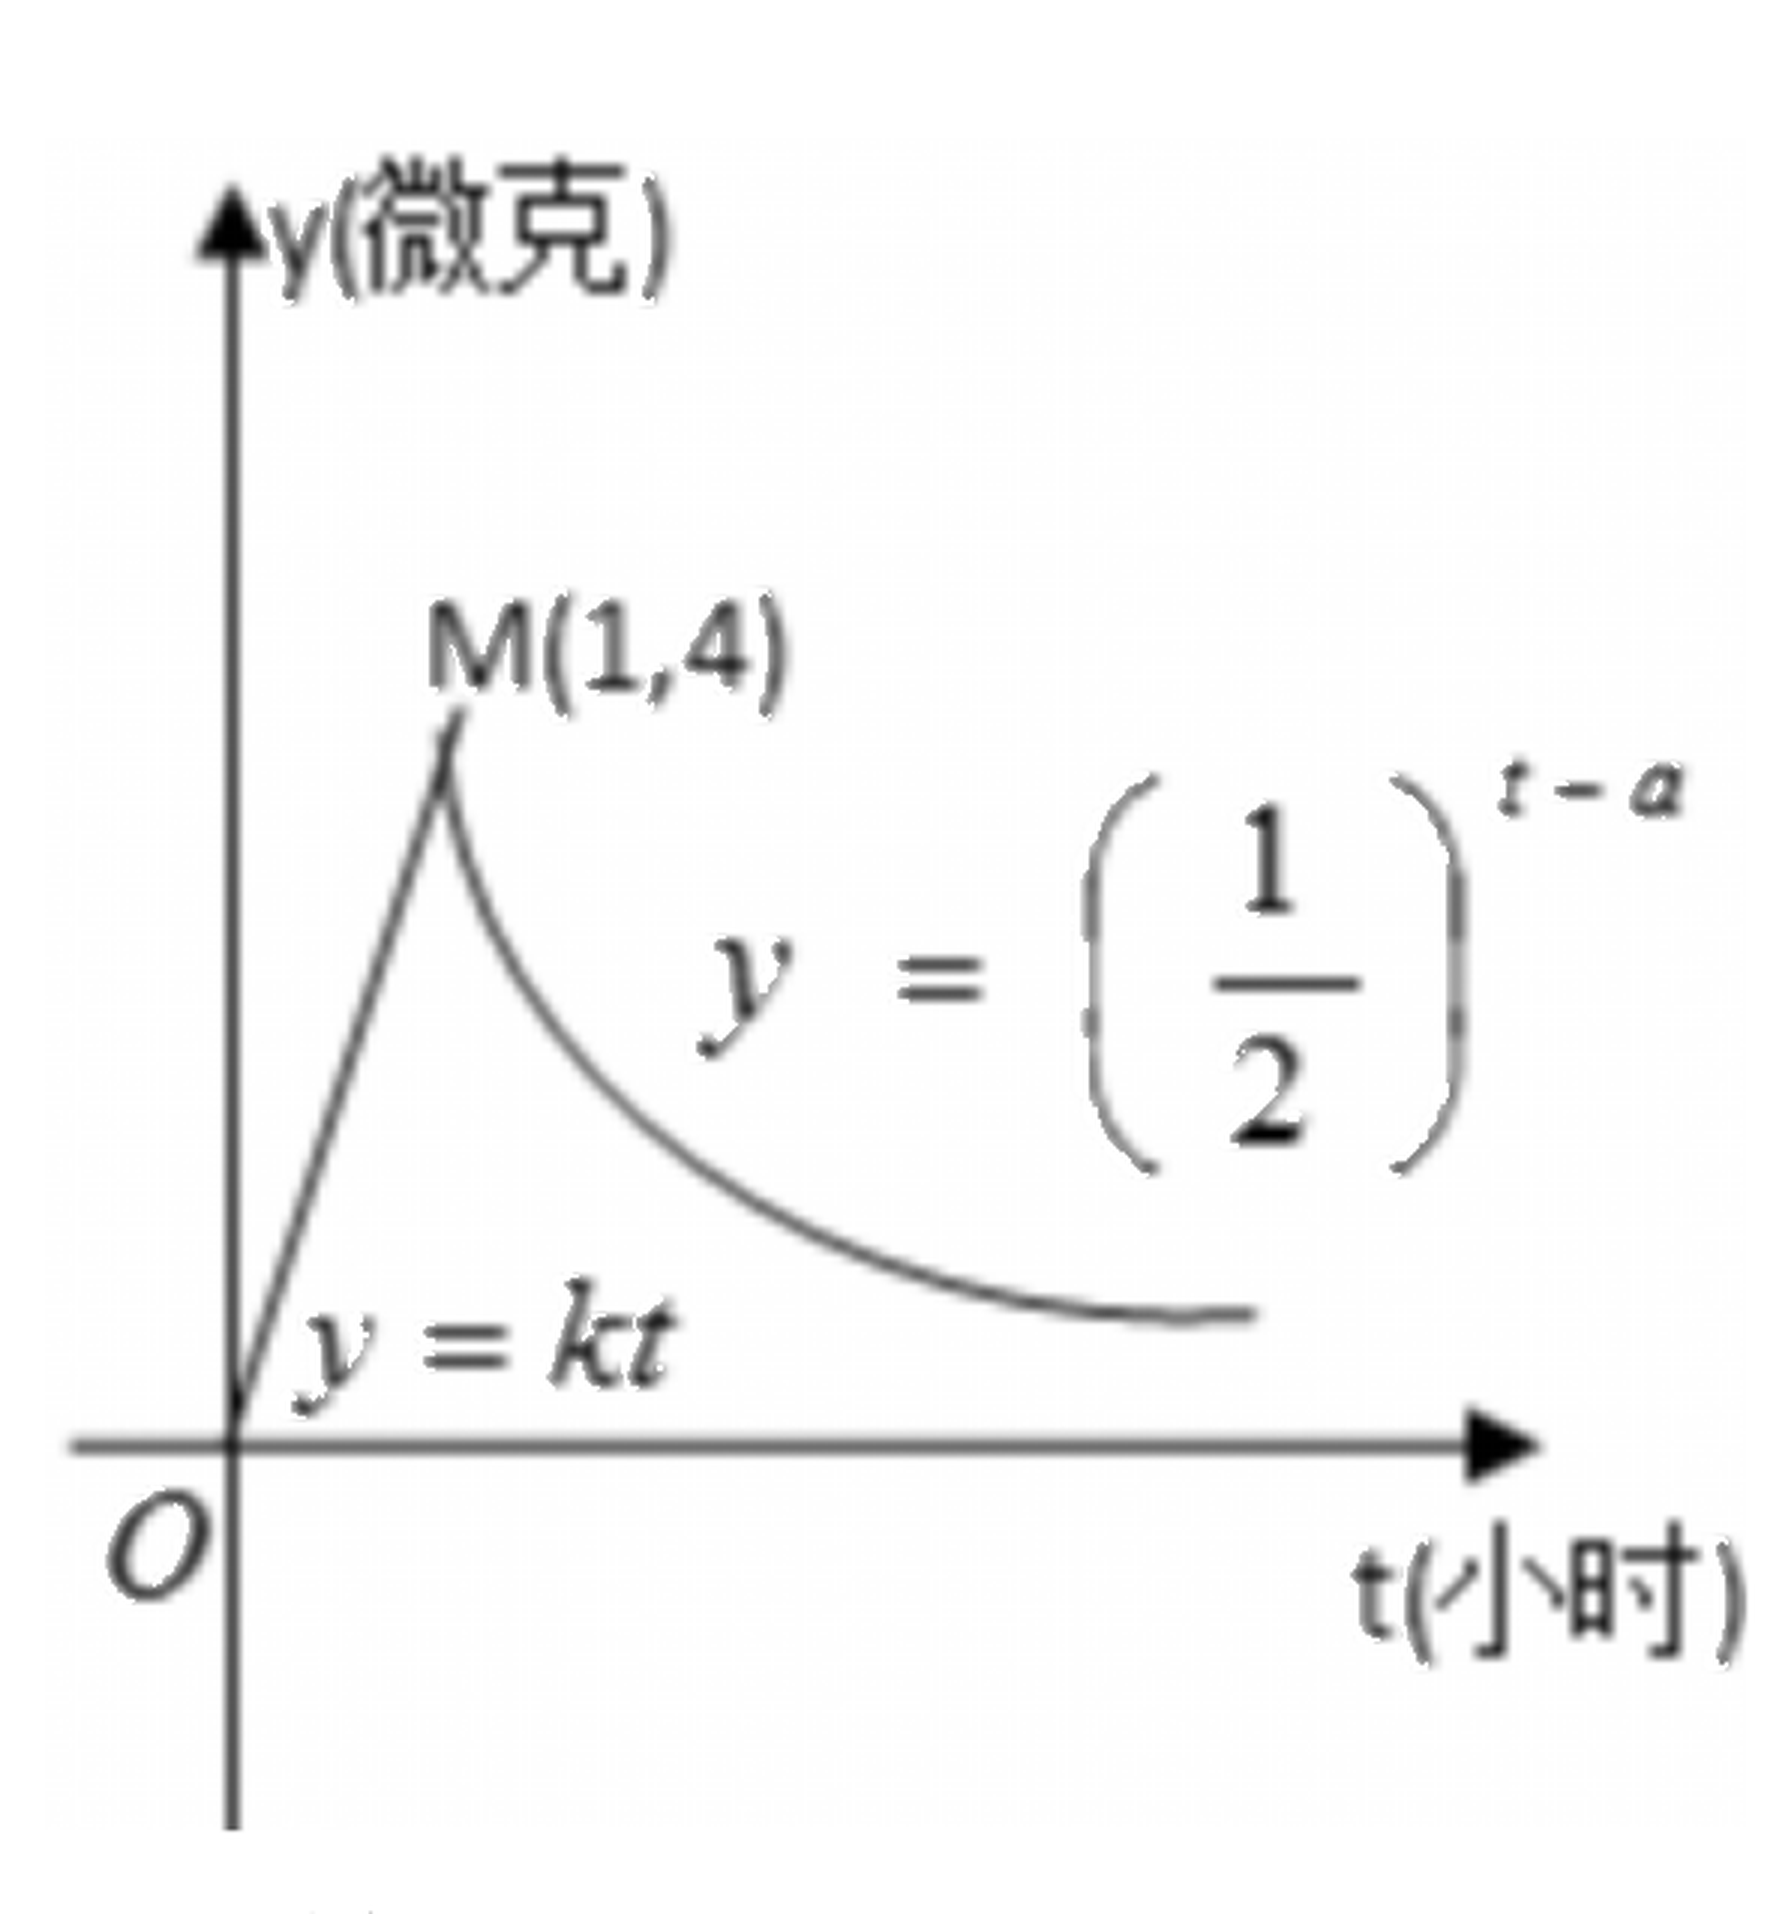
\includegraphics[width=0.42\textwidth]{figures/gao136_q20.png}
\end{center}

\ifanswer
\solbegin
\step{(1) 当 $0\leqslant t\leqslant1$ 时，函数图象是一条线段，由于过原点与点 $(1,4)$，所以 $k=4$，}
\step{其解析式为 $y=4t$，$0\leqslant t\leqslant1$；}
\step{当 $t\geqslant1$ 时，函数的解析式为 $y=\left(\dfrac12\right)^{t-a}$，}
\step{此时 $M(1,4)$ 在曲线上，将此点的坐标代入函数解析式得 $4=\left(\dfrac12\right)^{1-a}$，}
\step{解得 $a=3$；}
\step{(2) 由 (1) 得 $f(t)=\begin{cases}4t,0\leqslant t\leqslant1\\\left(\frac12\right)^{t-3},t>1\end{cases}$；}
\step{(3) 由 (2) 得，令 $f(t)\geqslant0.5$，即 $\begin{cases}4t\geqslant0.5,0\leqslant t\leqslant1\\\left(\frac12\right)^{t-3}\geqslant0.5,t>1\end{cases}$，所以 $\dfrac18\leqslant t\leqslant4$.}
\solend
\fi

\item 已知关于 $x$ 的不等式 $(kx-k^2-4)(x-4)>0$，其中 $k\in\R$.

(1) 当 $k=-1$，求不等式的解集 $A$；

(2) 当 $k$ 变化时，试求不等式的解集 $A$；

(3) 对于不等式解集 $A$，满足 $A\cap\Z=B$. 试探究集合 $B$ 能否为有限集，若能，求出使得集合 $B$ 中元素最少的 $k$ 的所有取值，并用列举法表示此时的集合 $B$，若不能，说明理由；

\ifanswer
\solbegin
\step{(1) 当 $k=-1$ 时，原不等式可化为 $(x+5)(x-4)<0$，}
\step{解得 $-5<x<4$，故不等式的解集为 $\{x\mid -5<x<4\}$；}
\step{(2) 当 $k=0$ 时，解集为 $\{x\mid x<4\}$，}
\step{当 $k>0$ 时，$\dfrac{k^2+4}{k}=k+\dfrac4k\geqslant4$，解集为 $\{x\mid x<4\text{ 或 }x>\dfrac{k^2+4}{k}\}$；}
\step{当 $k<0$ 时，解集为 $\{x\mid \dfrac{k^2+4}{k}<x<4\}$，}
\step{综上，当 $k=0$ 时，$A=\{x\mid x<4\}$，}
\step{当 $k>0$ 时，$A=\{x\mid x<4\text{ 或 }x>\dfrac{k^2+4}{k}\}$；}
\step{当 $k<0$ 时，$A=\{x\mid \dfrac{k^2+4}{k}<x<4\}$，}
\step{(3) 由 (2) 得当 $k\geqslant0$ 时，$B$ 为无限集，当 $k<0$ 时，$B$ 为有限集，}
\step{此时，$\dfrac{k^2+4}{k}=k+\dfrac4k\leqslant-4$，当且仅当 $k=-2$ 时取等号，}
\step{所以 $k=-2$ 时，$B$ 中元素最少，此时 $A=\{x\mid -4<x<4\}$，}
\step{所以 $B=\{-3,-2,-1,0,1,2,3\}$.}
\solend
\fi

\end{enumerate}

% 第 22 题是"四、附加题"首题且带 9cm 图块，守卫须放在 \bigsec 之前连节标题一起量，
% 否则"四、附加题"会孤立在页末（B 类，照 高一26／40／59 成例）
\needvspace{11cm}
\bigsec{四、附加题}

\begin{enumerate}
\setcounter{enumi}{21}

% 第 22 题四幅抛物线/坐标图选项是一整块，守卫放在 \item 之前
\needvspace{9cm}
\item 函数 $f(x)=\left(\dfrac12\right)^{\lvert x+1\rvert}$ 的图象大致为\mbox{（\quad）}

\keepwithprev
\begin{center}
% 四幅抛物线/坐标图选项取原卷 07 页截图去粉色水印，按原卷 2x2 排布合并为一张
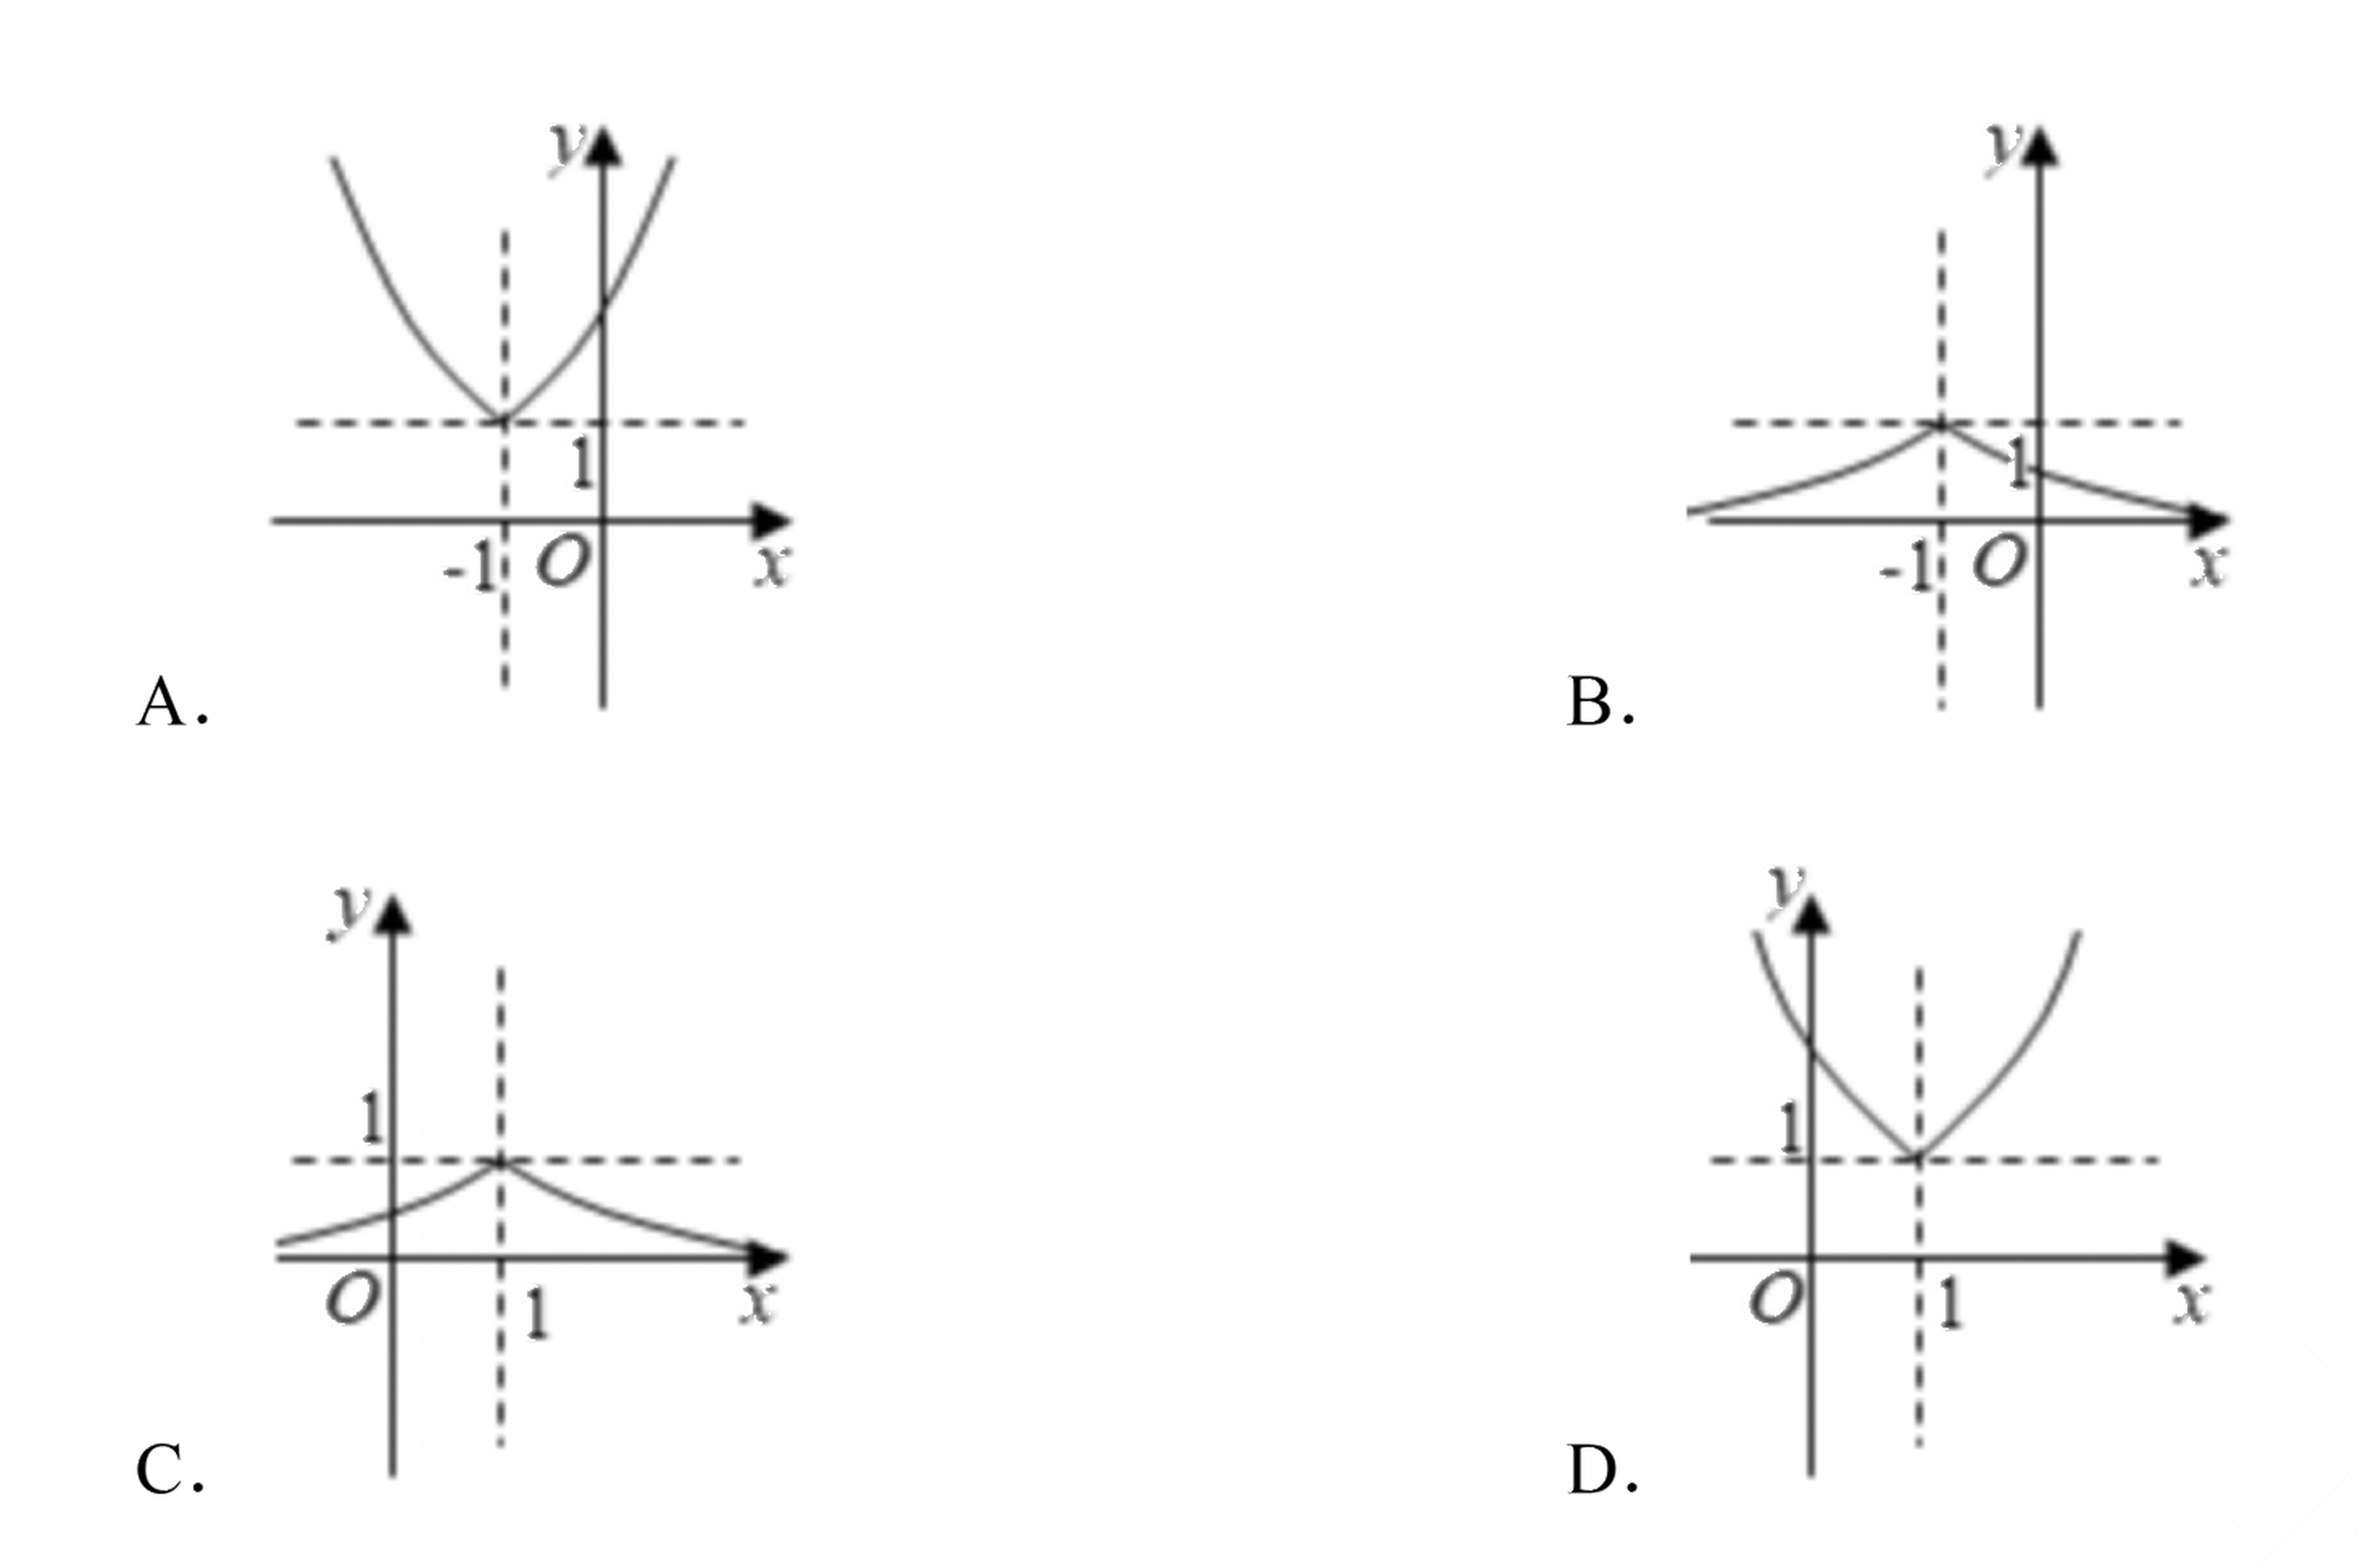
\includegraphics[width=0.80\textwidth]{figures/gao136_q22.png}
\end{center}

\ifanswer
\ans{$B$}
\fi

\end{enumerate}

\end{document}
"
%
% ① 原始材料：微信公众号"魔都数学加油站"文章，作者破晓，2026-11-15 18:04 发布；
% 连载"27学年高一136"，原文标题"27学年高一136——2026-2027年上海市三林中学高一上期中"；
% 原文链接：https://mp.weixin.qq.com/s/jaMzqMm6pDvcT0yM0d7eaQ。
% 正文为 7 张 PNG 页（01、04、06 为 4762x6735；02、03、05、07 为 2560x3620，
% 同一篇各页分辨率不同，逐页按各自分辨率裁图核对），题目下印有【答案】或【解析】，为讲评版。
% 题目、解析均据原图转录；卷面粉红色水印"魔都数学加油站"及公众号页脚未录入。
% 全卷 3 幅插图：第 13 题四幅坐标图选项（03 页）、第 20 题药物浓度折线/曲线图（05 页）、
% 第 22 题四幅抛物线/坐标图选项（07 页），均取原卷截图去粉色水印、去色、LANCZOS 放大，
% 四幅选项按原卷 2x2 排布合并为一张；图前按惯例加 \needvspace 守卫。
%
% 卷首标题：原卷印作"2026-2027 年三林中学高一上期中"（公众号标题中的"上海市"
% 卷面标题行没有，本稿照卷面），年份区间按全稿惯例排 en dash；原卷未印副标题，
% 本卷为期中卷、跨集合与常用逻辑用语／不等式／函数三章，按题目内容标为
% "集合与常用逻辑用语、不等式、函数"（与 125／126／128／129／131／132／133 同期中卷口径相同）：
% 集合与逻辑见 Q3、Q6、Q10、Q12、Q16、Q18、Q21，不等式见 Q5、Q7、Q8、Q9、Q14、Q15，
% 函数（幂函数、指数／对数、基本不等式应用）见 Q4、Q11、Q13、Q17、Q19、Q20、Q22。
%
% 题号体例：本卷共 20 题——一、填空题 3—12（10 题）、二、选择题 13—16（4 题）、
% 三、解答题 17—21（5 题）、四、附加题 22（1 题）。四节分别
% \setcounter{enumi}{2}／{12}／{16}／{21}。
%
% ② 与原卷的排版差异：
%   ① 原文从第 3 题起，本稿保留原题号；末节"四、附加题"另起 \bigsec，题号续到 22；
%   ② 原卷每题下直接印【答案】或【解析】，本稿按全稿惯例置于答案版；第 3、4、6 题只印
%      【答案】、无【解析】，提 \ans{}；第 14 题答案 C 印在题干括号内、无【解析】，按
%      高一53／高一108／高一132／高一133 成例括号留空、另提 \ans{$C$}；第 22 题答案 B
%      印在题干括号内、无【解析】，同例提 \ans{$B$}；第 13、15、16 题答案在解析末句
%      "故选 …"，括号内留空、不另提 \ans{}；其余各题印【解析】、无独立答案段；
%   ③ 原卷未印副标题，本稿按"知识模块"口径补出；
%   ④ 原卷填空横线按全稿惯例排为 \blankline[4.4em]；选择题括号排 \mbox{（\quad）}、
%      每个选项段前按惯例加 \keepwithprev（四幅图选项那一枚放在 \begin{center} 之前）；
%      解答题不留作答区、不加 \anspace（原卷为讲评版，与 129／131／132／133 同）；
%   ⑤ 原卷数集排斜体 $R$／$R^+$／$Z$，按全稿惯例改 \R／\R^+／\Z；空集记号 \varnothing；
%      绝对值排 \lvert…\rvert，集合描述竖线排 \mid；不等号按全稿惯例排 \leqslant／\geqslant；
%   ⑥ 子题标号 (1)(2)(3) 原卷用半角括号，照录；圈数字 ①②③④ 照录；第 12 题甲／乙／丙
%      三行与第 14 题四个编号不等式照录；
%   ⑦ 数学式内半角逗号照录（如 Q4"$a>0,a\neq1$"、Q6"$\{(-2,4),(1,1)\}$"、
%      Q7"$a=2+3=5,b=2\times3=6$"、Q11"$x_1,x_2$"、Q12"$m,n\in R^+$"、
%      Q15"$a>1,b\geq0$"、Q18"$B=(2a,a+1)$"、Q20"$4t,0\leq t\leq1$"、
%      Q21"$\{-3,-2,-1,0,1,2,3\}$"）；原卷行末西文句点照录，行中全角逗号照录；
%   ⑧ 三幅插图：第 13 题四幅坐标图选项合并裁为一张 \includegraphics（题前 \needvspace{9cm}）；
%      第 20 题折线/曲线图取 05 页截图（0.42\textwidth）；第 22 题四幅抛物线/坐标图选项合并
%      裁为一张（题前 \needvspace{9cm}）。第 13、22 题分别是"二、选择题""四、附加题"的首题
%      且带大图块，另在两处 \bigsec 之前各加 \needvspace{11cm} 连节标题一起量，避免节标题
%      孤立在页末（切页审计 B 类；照 高一26／40／59 成例）。第 20 题图不是节首题、三版试排
%      图均与题干同页，加 7cm 守卫反会多出一张只有两行正文的稀疏页，故不另加守卫；
%      三版切页审计均"合计异常：无"（试卷 4 页／紧凑 4 页／答案 6 页）；
%   ⑨ 跨页续印按题合并：Q16 题干在 03 页、括号与选项及【解析】在 04 页；Q19 题干在 04 页、
%      (2) 与【解析】在 05 页；Q20 (3)【解析】在 06 页；Q22 四幅图在 07 页；本稿按题连排；
%   ⑩ 题干中的中文弯引号按原卷照录，注释内一律 ASCII 引号；原卷"图像／图象"两种写法混用，
%      逐处照录（Q4、Q19 作"图像"，Q13、Q15、Q20、Q22 作"图象"）；
%   ⑪ 附加题节：原卷印"四、附加题"，本稿用 \bigsec{四、附加题} 另起一节、
%      \setcounter{enumi}{21}，顶层 1 个 \item（与 高一09／15／16／22／35／39／47／61 同口径）；
%      Q22 只印括号内答案、提 \ans{}，不计入 \step 账。
%
% 判别式字形：全卷仅第 9 题【解析】cases 块出现判别式"$\Delta=a^2-8a<0$"，原卷印
%   等腰、偏高的三角 $\Delta$，逐处放大核对并照录 \Delta；全卷未出现扁等边三角 \triangle。
%
% 子集符号：第 18 题 (2) 题干"$B\subseteq A$"与【解析】"$B\subseteq A$"两处原卷均印
%   带下划线 $\subseteq$，逐处放大核对、照录 \subseteq；全卷未出现单线 \subset。
%
% 原卷存疑照录（均照录未改，正文对应处另有 % 注）：
%   第 12 题乙行"$\dfrac{m+n}{mm}=\dfrac1{mn}$"前一分母印作 $mm$（后一处作 $mn$），照录；
%   第 12 题【解析】"$\geqslant\dfrac1{100}\left[a^2+1+2\sqrt{a^2}\right]$"保留 $\sqrt{a^2}$
%      未化简为 $a$，照录；
%   第 13 题【解析】"排除 BC"与"排除 D"连写选项字母，照录；
%   第 18 题 (2)【解析】末行"所以实数 $a$ 的取值范围 $(-\infty,-2]\cup[\frac12,1)$"
%      "取值范围"后脱"是／为"字，照录；
%   第 21 题 (3) 题干"求出使得集合 $B$ 中元素最少的 $k$ 的所有取值"而【解析】只给出
%      $k=-2$ 一处，措辞照录。
%
% 行数复核：逐题数 \step 条数，合计 51 条（Q3：0；Q4：0；Q5：2；Q6：0；Q7：2；Q8：1；
% Q9：1；Q10：4；Q11：1；Q12：4；Q13：2；Q14：0；Q15：2；Q16：3；Q17：1；Q18：5；
% Q19：4；Q20：7；Q21：12；Q22：0），与原卷印刷行逐题相等（cases 块作一个印刷行计）。
% 第 3、4、6、14、22 题只印【答案】、提 \ans{}，不计入 \step 账；第 13、15、16 题答案在
% 解析末句，括号内留空、不另提 \ans{}。
%
\documentclass[a4paper,11pt]{article}
\usepackage{common}

\begin{document}

\examtitlest[3]{2026--2027 年三林中学高一上期中}{集合与常用逻辑用语、不等式、函数}

\bigsec{一、填空题}

\begin{enumerate}
\setcounter{enumi}{2}

\item 用反证法证明命题“若 $x+y\neq5$，则 $x\neq2$ 或 $y\neq3$”为真命题时，第一个步骤是\blankline[4.4em].

\ifanswer
\ans{假设 $x=2$ 且 $y=3$}
\fi

\item 函数 $y=a^{x-1}+1(a>0,a\neq1)$ 的图像恒过定点 $A$，则点的坐标是\blankline[4.4em].

\ifanswer
\ans{$(1,2)$}
\fi

\item 已知 $x>1$，则 $x+\dfrac4{x-1}$ 的最小值是\blankline[4.4em].

\ifanswer
\solbegin
\step{由 $x>1$，得 $x-1>0$，则 $x+\dfrac4{x-1}=x-1+\dfrac4{x-1}+1\geqslant2\sqrt{(x-1)\cdot\dfrac4{x-1}}+1=5$，}
\step{当且仅当 $x-1=\dfrac4{x-1}$ 即 $x=3$ 时取等号，取得最小值 $5$.}
\solend
\fi

\item 已知集合 $A=\{(x,y)\mid y=x^2\}$，集合 $B=\{(x,y)\mid y=2-x\}$，求 $A\cap B=$\blankline[4.4em].

\ifanswer
\ans{$\{(-2,4),(1,1)\}$}
\fi

\item 已知一元二次不等式 $x^2-ax+b<0$ 的解集为 $(2,3)$，则不等式 $bx^2-ax+1>0$ 的解集是\blankline[4.4em].

\ifanswer
\solbegin
\step{$a=2+3=5,b=2\times3=6$，则 $bx^2-ax+1>0$ 即 $6x^2-5x+1>0$，}
\step{即 $(3x-1)(2x-1)>0$，解集为 $\left(-\infty,\dfrac13\right)\cup\left(\dfrac12,+\infty\right)$.}
\solend
\fi

\item 不等式 $(x+2)^3<(5-2x)^3$ 的解集为\blankline[4.4em].

\ifanswer
\solbegin
\step{由 $(x+2)^3<(5-2x)^3$ 得 $x+2<5-2x$，故解集为 $(-\infty,1)$.}
\solend
\fi

\item 若关于 $x$ 的不等式 $ax^2-ax+2>0$ 的解集为 $\R$，则实数 $a$ 的取值范围是\blankline[4.4em].

\ifanswer
\solbegin
\step{由题意得 $a=0$ 或 $\begin{cases}a>0\\\Delta=a^2-8a<0\end{cases}$，所以 $0\leqslant a<8$.}% 判别式原卷印高三角 $\Delta$，照录
\solend
\fi

\item 已知关于 $x$ 的不等式 $\lvert x+3\rvert+\lvert x-a\rvert\geqslant5$ 恒成立，则实数 $a$ 的取值范围为\blankline[4.4em].

\ifanswer
\solbegin
\step{因为 $\lvert x+3\rvert+\lvert x-a\rvert\geqslant\lvert x-a-x-3\rvert=\lvert 3+a\rvert$，}
\step{要使 $\lvert x+3\rvert+\lvert x-a\rvert\geqslant5$ 恒成立，则 $\lvert a+3\rvert\geqslant5$ 即可，}
\step{所以 $a+3\geqslant5$ 或 $a+3\leqslant-5$，解得 $a\geqslant2$ 或 $a\leqslant-8$，}
\step{即实数 $a$ 的取值范围是 $(-\infty,-8]\cup[2,+\infty)$.}
\solend
\fi

\item 若方程 $\lg^2 x-2\lg x-2=0$ 的两个解为 $x_1,x_2$，求 $\log_{x_1}x_2+\log_{x_2}x_1$ 的值为\blankline[4.4em].

\ifanswer
\solbegin
\step{$\log_{x_1}x_2+\log_{x_2}x_1=\dfrac{\lg x_2}{\lg x_1}+\dfrac{\lg x_1}{\lg x_2}=\dfrac{(\lg x_1+\lg x_2)^2-2\lg x_1\lg x_2}{\lg x_1\lg x_2}=-4$.}
\solend
\fi

\item 三个同学对问题“已知 $m,n\in \R^+$，且 $m+n=1$，求 $\dfrac1m+\dfrac1n$ 的最小值”提出各自的解题思路：

思路：

甲：$\dfrac1m+\dfrac1n=\dfrac{m+n}{m}+\dfrac{m+n}{n}=2+\dfrac nm+\dfrac mn$，可用基本不等式求解；

乙：$\dfrac1m+\dfrac1n=\dfrac{m+n}{mm}=\dfrac1{mn}=\dfrac1{m(1-m)}$，可用二次函数配方法求解；% 原卷前一分母印作 $mm$，照录

丙：$\dfrac1m+\dfrac1n=\left(\dfrac1m+\dfrac1n\right)(m+n)=2+\dfrac nm+\dfrac mn$，可用基本不等式求解；参考上述解题思路，

可求得当 $x=$\blankline[4.4em]时，$y=\dfrac{a^2}{x^2}+\dfrac1{100-x^2}$（$0<x<10$，$a>0$）有最小值.

\ifanswer
\solbegin
\step{$y=\dfrac{a^2}{x^2}+\dfrac1{100-x^2}=\left(\dfrac{a^2}{x^2}+\dfrac1{100-x^2}\right)[x^2+(100-x^2)]\times\dfrac1{100}$}
\step{$=\dfrac1{100}\left[a^2+1+\dfrac{x^2}{100-x^2}+\dfrac{a^2(100-x^2)}{x^2}\right]\geqslant\dfrac1{100}\left[a^2+1+2\sqrt{a^2}\right]$}% 原卷保留 $\sqrt{a^2}$ 未化简，照录
\step{当且仅当 $\dfrac{x^2}{100-x^2}=\dfrac{a^2(100-x^2)}{x^2}$，即 $x=\sqrt{\dfrac{100a}{a+1}}$ 时，}
\step{$y=\dfrac{a^2}{x^2}+\dfrac1{100-x^2}(0<x<10,a>0)$ 有最小值.}
\solend
\fi

\end{enumerate}

% 第 13 题是"二、选择题"首题且带 9cm 图块，守卫须放在 \bigsec 之前连节标题一起量，
% 否则"二、选择题"会孤立在页末（B 类，照 高一26／40／59 成例）
\needvspace{11cm}
\bigsec{二、选择题}

\begin{enumerate}
\setcounter{enumi}{12}

% 第 13 题四幅坐标图选项是一整块，守卫放在 \item 之前
\needvspace{9cm}
\item 下列图象中，最符合函数 $y=x^{\frac54}$ 的图象的是\mbox{（\quad）}

\keepwithprev
\begin{center}
% 四幅坐标图选项取原卷 03 页截图去粉色水印，按原卷 2x2 排布合并为一张
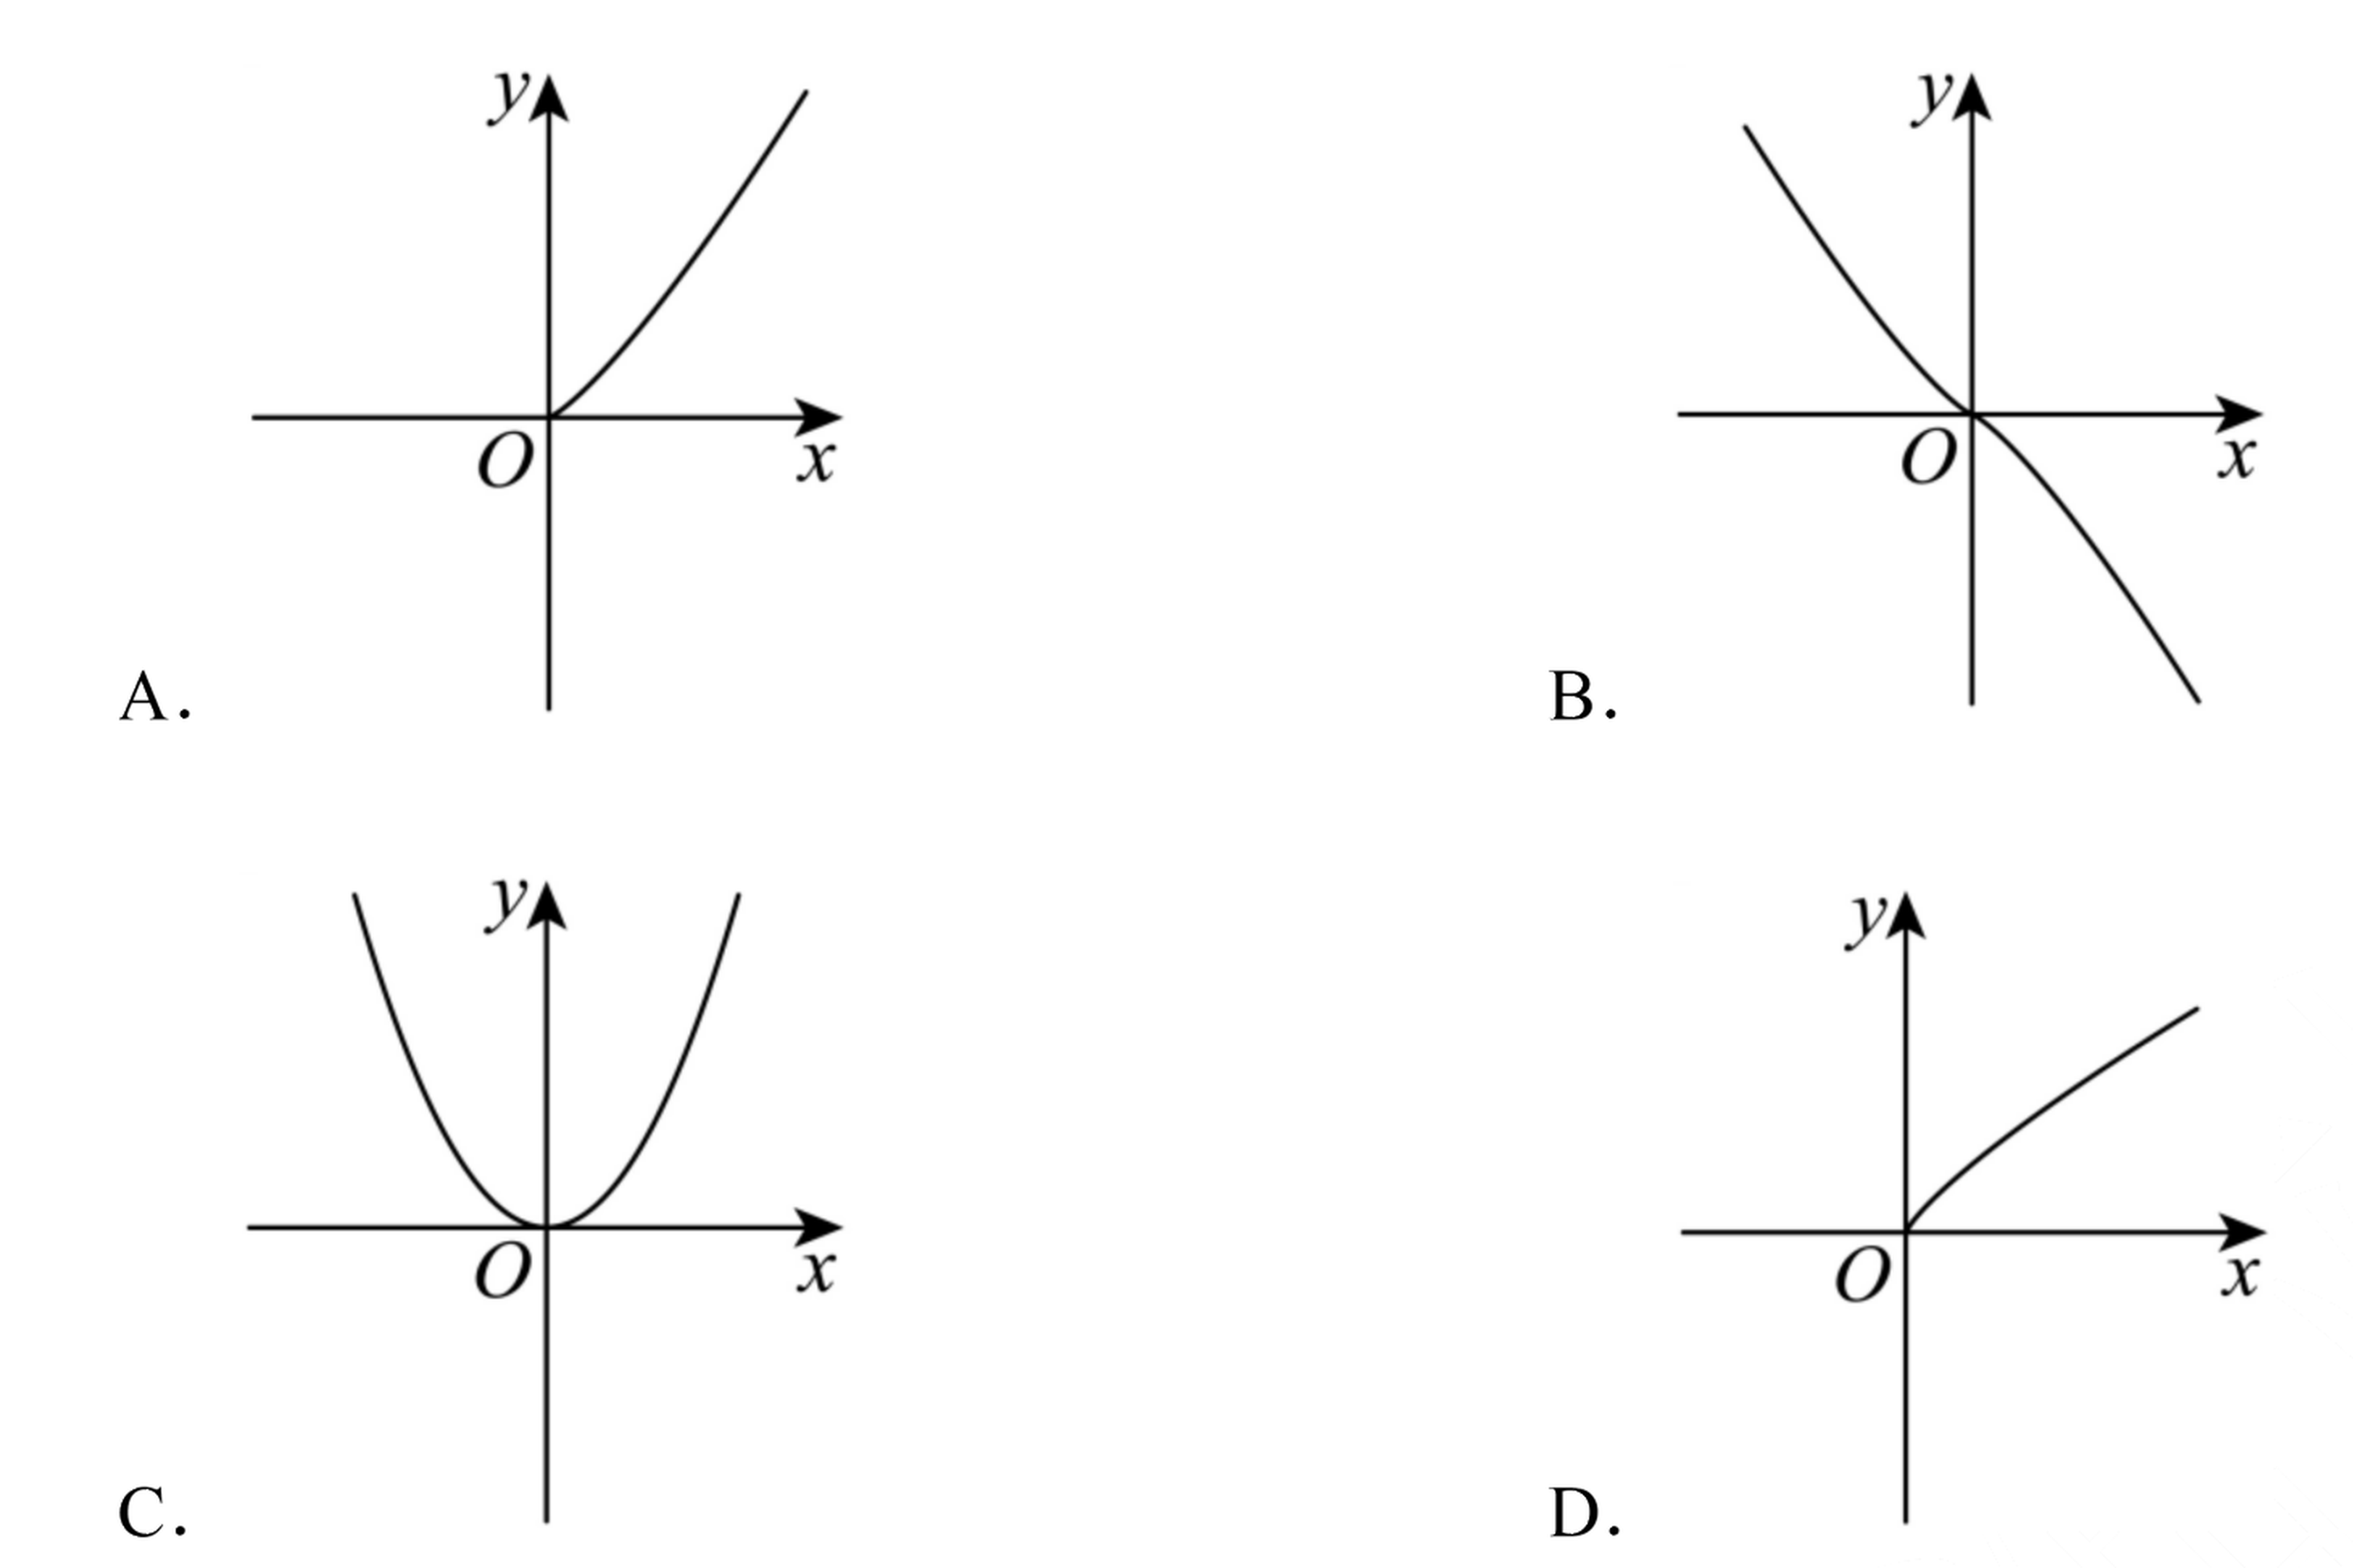
\includegraphics[width=0.80\textwidth]{figures/gao136_q13.png}
\end{center}

\ifanswer
\solbegin
\step{由 $y=x^{\frac54}=\sqrt[4]{x^5}$，函数的定义域为 $[0,+\infty)$，排除 BC，}% 原卷"排除 BC"连写，照录
\step{因为 $\dfrac54>1$，所以函数 $y=x^{\frac54}$ 的图象呈现下凸的趋势，排除 D. 故选 $A$.}
\solend
\fi

\item 下列不等式① $a+\dfrac1a\geqslant2$；② $a^2+4\geqslant4a$；③ $\left\lvert\dfrac ba+\dfrac ab\right\rvert\geqslant2$；④ $\dfrac{2a^2b^2}{a^2+b^2}\leqslant ab$；其中恒成立的是\mbox{（\quad）}

\keepwithprev
A. ①④\qquad B. ③④\qquad C. ②③\qquad D. ①②

\ifanswer
\ans{$C$}
\fi

\item 函数 $y=a^x+b-1(a>0,a\neq1)$ 单调递增且图象不经过第四象限，则 $a,b$ 满足的条件为\mbox{（\quad）}

\keepwithprev
A. $a>1,b\leqslant1$\qquad B. $a>1,b\geqslant0$\qquad C. $0<a<1,b\leqslant1$\qquad D. $0<a<1,b\geqslant1$

\ifanswer
\solbegin
\step{因为函数 $y=a^x+b-1$ 单调递增，所以 $a>1$，}
\step{图象不经过第四象限，则 $x=0$ 时，$y=b\geqslant0$，所以 $a>1,b\geqslant0$，故选 $B$.}
\solend
\fi

\item 设关于 $x$ 的不等式 $\dfrac{ax-1}{x^2-a}<0$ 的解集为 $S$，且 $3\in S$，$4\notin S$，则实数 $a$ 的取值范围为\mbox{（\quad）}

\keepwithprev
A. $(-\infty,-\sqrt3)\cup\left(\dfrac13,\sqrt3\right)$\qquad B. $\left(-\infty,\dfrac14\right)\cup(16,+\infty)$

C. $\left[\dfrac14,\dfrac13\right)\cup(9,16]$\qquad D. 不能确定

\ifanswer
\solbegin
\step{若 $3\in S$，则 $\dfrac{3a-1}{9-a}<0$，解得 $a\in\left(-\infty,\dfrac13\right)\cup(9,+\infty)$，}
\step{若 $4\notin S$，则 $16-a=0$ 或 $\dfrac{4a-1}{16-a}\geqslant0$，解得 $a\in\left[\dfrac14,16\right]$，}
\step{故实数 $a$ 的取值范围为 $\left[\dfrac14,\dfrac13\right)\cup(9,16]$，故选 $C$.}
\solend
\fi

\end{enumerate}

\bigsec{三、解答题}

\begin{enumerate}
\setcounter{enumi}{16}

\item 计算：(1) 计算 $\dfrac{\lg8+\lg125-\lg2-\lg5}{\lg\sqrt{10}\cdot\lg0.1}$；(2) 若 $a^{2x}=2(a>0)$，求 $\dfrac{a^{3x}+a^{-3x}}{a^x+a^{-x}}$.

\ifanswer
\solbegin
\step{(1) 原式 $=\dfrac{2-1}{\frac12\cdot(-1)}=-2$；(2) 原式 $=a^{2x}-1+a^{-2x}=2-1+\dfrac12=\dfrac32$.}
\solend
\fi

\item 不等式 $\dfrac{x-1}{x+1}\geqslant0$ 的解集为 $A$，不等式 $(x-a-1)(2a-x)>0(a<1)$ 的解集为 $B$.

(1) 求集合 $A$；

(2) 若 $B\subseteq A$，求实数 $a$ 的取值范围.

\ifanswer
\solbegin
\step{(1) $A=(-\infty,-1)\cup[1,+\infty)$.}
\step{(2) 由 $(x-a-1)(2a-x)>0(a<1)$，得 $(x-a-1)(x-2a)<0(a<1)$，}
\step{因为 $a<1$，所以 $a+1>2a$，所以 $B=(2a,a+1)$，}
\step{因为 $B\subseteq A$，所以 $2a\geqslant1$ 或 $a+1\leqslant-1$，即 $a\geqslant\dfrac12$ 或 $a\leqslant-2$，}
\step{而 $a<1$，所以实数 $a$ 的取值范围 $(-\infty,-2]\cup\left[\dfrac12,1\right)$.}% 原卷"取值范围"后脱"是／为"，照录
\solend
\fi

\item 已知幂函数 $y=x^m(m\in\R)$ 经过点 $\left(4,\dfrac12\right)$.

(1) 求此幂函数的表达式和定义域；

(2) 已知点 $A(a+2,y_1)$，点 $B(3-2a,y_2)(a\in\R)$ 在此幂函数的图像上，且满足 $y_1<y_2$，求实数 $a$ 的取值范围.

\ifanswer
\solbegin
\step{(1) 幂函数 $y=x^m(m\in\R)$ 经过点 $\left(4,\dfrac12\right)$，所以 $4^m=\dfrac12\Rightarrow m=-\dfrac12$，}
\step{所以 $f(x)=x^{-\frac12}$，定义域为 $(0,+\infty)$.}
\step{(2) 由于函数 $f(x)$ 在其定义域 $(0,+\infty)$ 上严格减，}
\step{由 $y_1<y_2$，得 $a+2>3-2a\geqslant0\Rightarrow a\in\left(\dfrac13,\dfrac32\right]$.}
\solend
\fi

% 第 20 题图取 05 页截图（0.42\textwidth、高约 6cm）。试排 \item 前加 7cm 守卫会多出
% 一张只有两行正文的稀疏页，且三版不加守卫时图均与题干、【解析】同页，故不另加守卫
\item 某医药研究所开发一种抗甲流新药，如果成年人按规定的剂量服用，据监测：服药后每毫升血液中的含药量 $y$（微克）与时间 $t$（小时）之间近似满足如图所示的曲线.

(1) 结合图，求 $k$ 与 $a$ 的值；

(2) 写出服药后 $y$ 与 $t$ 之间的函数关系式 $y=f(t)$；

(3) 据进一步测定：每毫升血液中含药量不少于 $0.5$ 微克时治疗疾病有效，求服药一次治疗有效的时间范围？

\begin{center}
% 图取原卷 05 页截图去粉色水印、去色，3x LANCZOS 放大
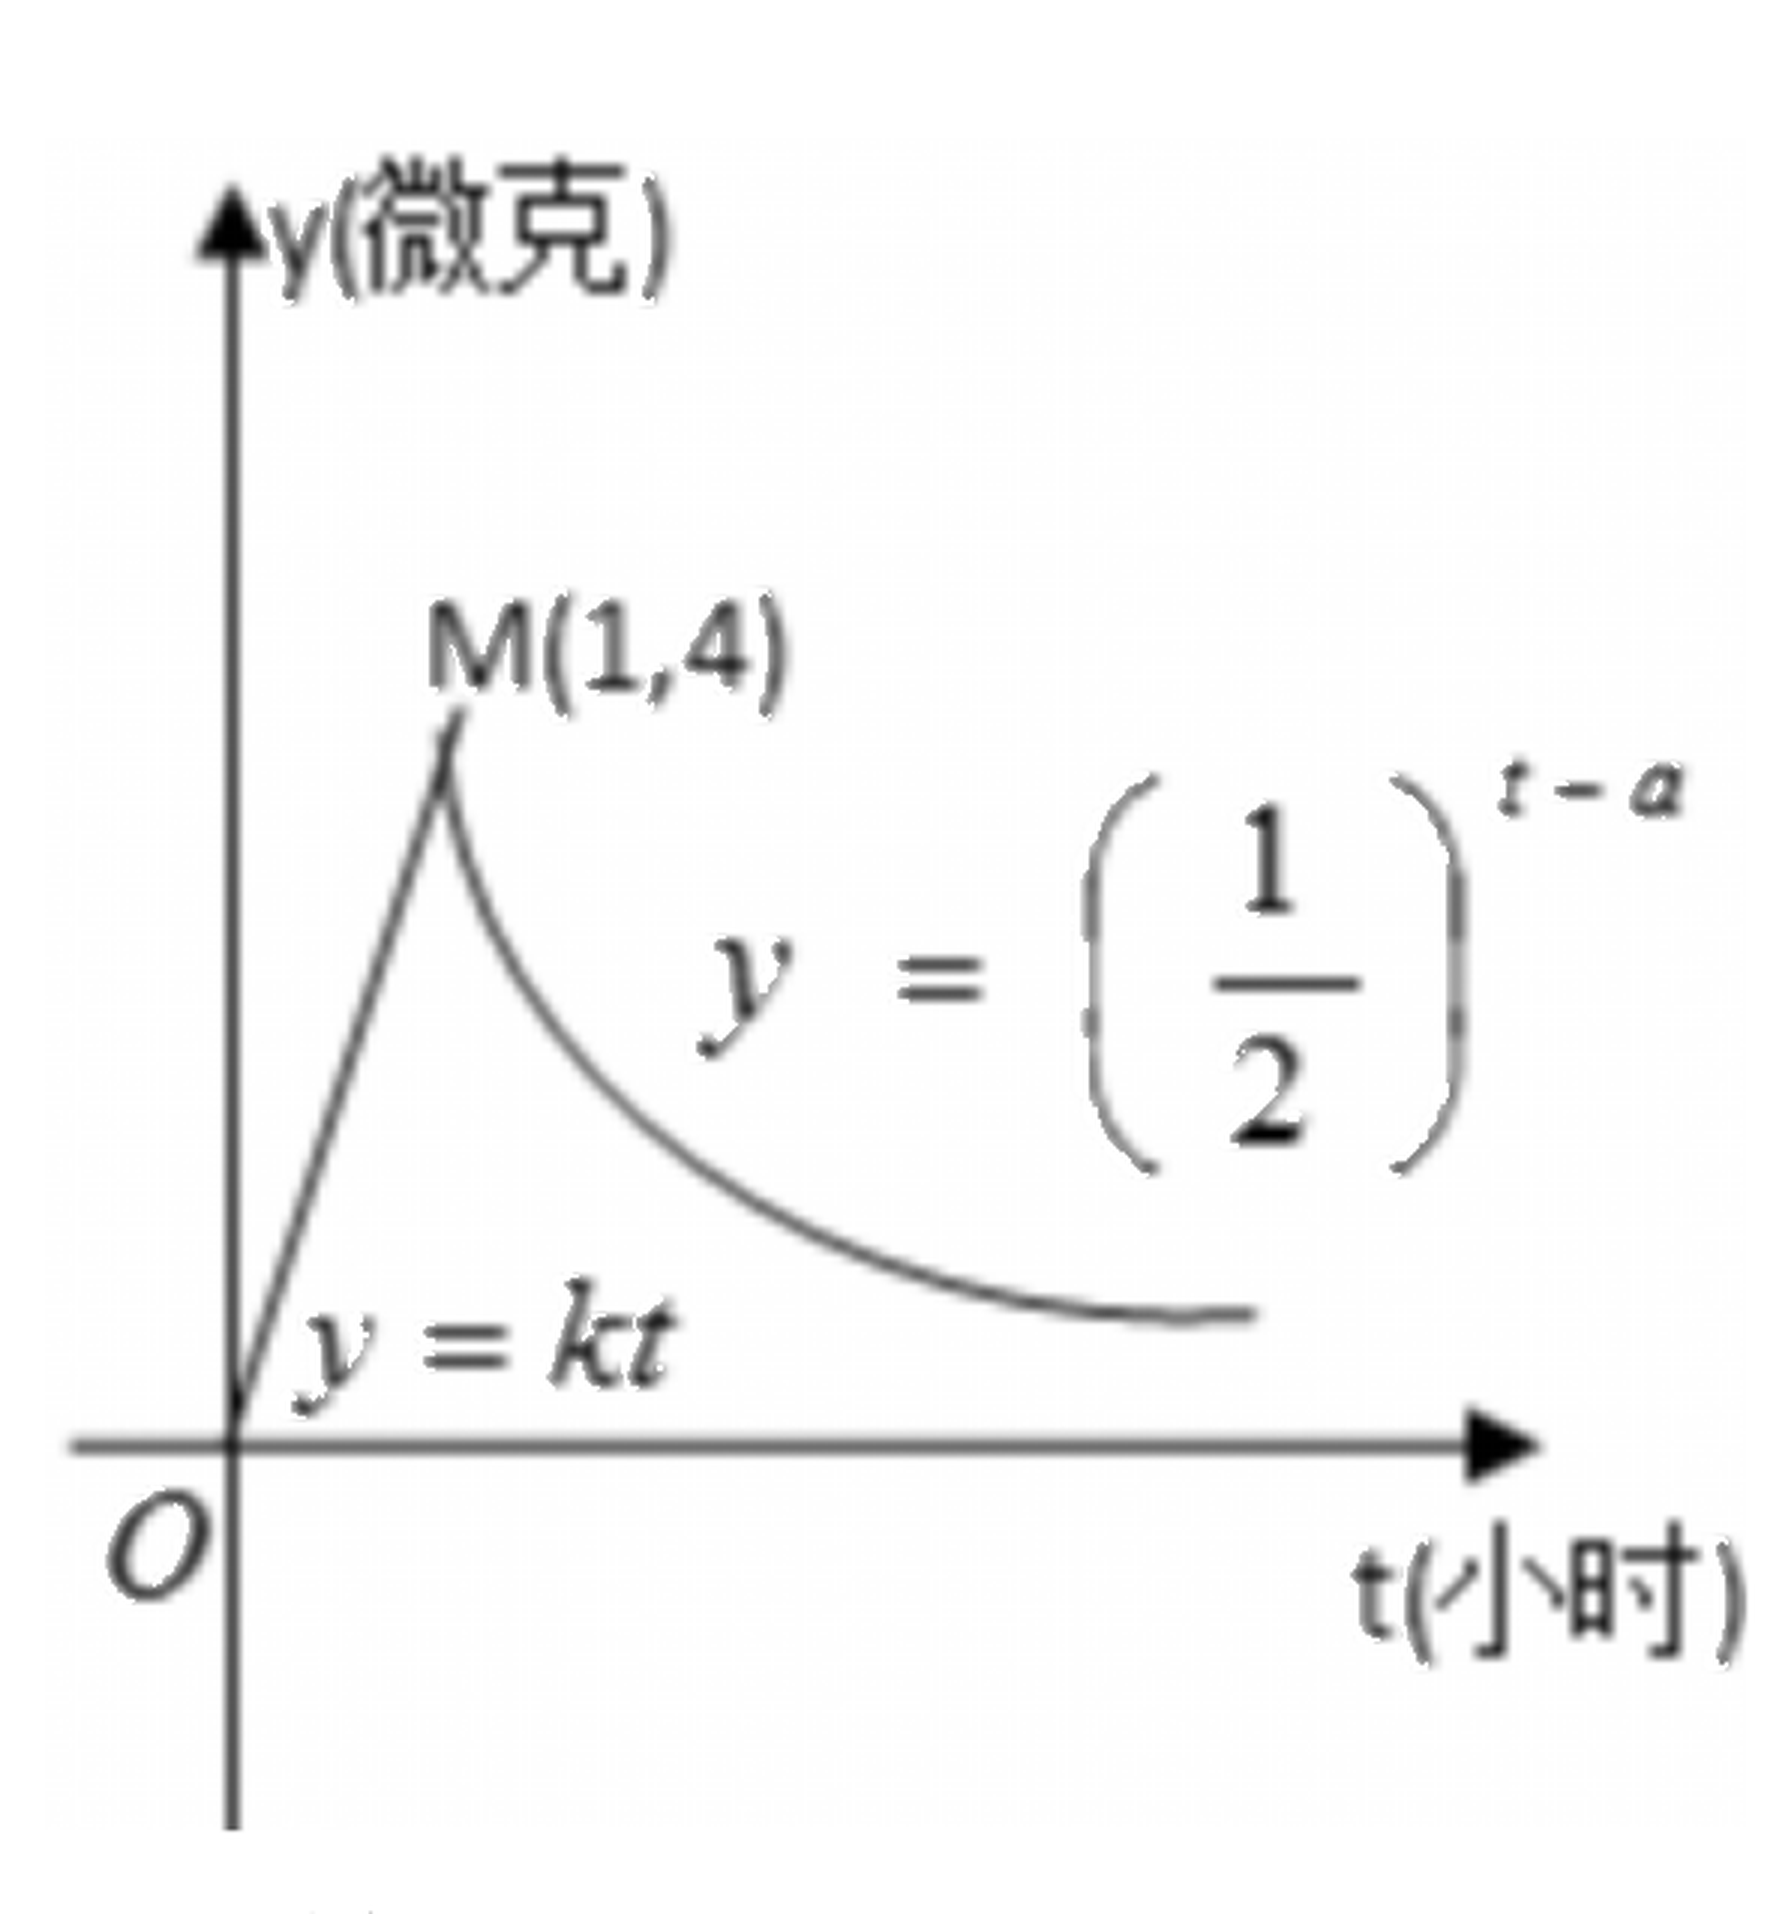
\includegraphics[width=0.42\textwidth]{figures/gao136_q20.png}
\end{center}

\ifanswer
\solbegin
\step{(1) 当 $0\leqslant t\leqslant1$ 时，函数图象是一条线段，由于过原点与点 $(1,4)$，所以 $k=4$，}
\step{其解析式为 $y=4t$，$0\leqslant t\leqslant1$；}
\step{当 $t\geqslant1$ 时，函数的解析式为 $y=\left(\dfrac12\right)^{t-a}$，}
\step{此时 $M(1,4)$ 在曲线上，将此点的坐标代入函数解析式得 $4=\left(\dfrac12\right)^{1-a}$，}
\step{解得 $a=3$；}
\step{(2) 由 (1) 得 $f(t)=\begin{cases}4t,0\leqslant t\leqslant1\\\left(\frac12\right)^{t-3},t>1\end{cases}$；}
\step{(3) 由 (2) 得，令 $f(t)\geqslant0.5$，即 $\begin{cases}4t\geqslant0.5,0\leqslant t\leqslant1\\\left(\frac12\right)^{t-3}\geqslant0.5,t>1\end{cases}$，所以 $\dfrac18\leqslant t\leqslant4$.}
\solend
\fi

\item 已知关于 $x$ 的不等式 $(kx-k^2-4)(x-4)>0$，其中 $k\in\R$.

(1) 当 $k=-1$，求不等式的解集 $A$；

(2) 当 $k$ 变化时，试求不等式的解集 $A$；

(3) 对于不等式解集 $A$，满足 $A\cap\Z=B$. 试探究集合 $B$ 能否为有限集，若能，求出使得集合 $B$ 中元素最少的 $k$ 的所有取值，并用列举法表示此时的集合 $B$，若不能，说明理由；

\ifanswer
\solbegin
\step{(1) 当 $k=-1$ 时，原不等式可化为 $(x+5)(x-4)<0$，}
\step{解得 $-5<x<4$，故不等式的解集为 $\{x\mid -5<x<4\}$；}
\step{(2) 当 $k=0$ 时，解集为 $\{x\mid x<4\}$，}
\step{当 $k>0$ 时，$\dfrac{k^2+4}{k}=k+\dfrac4k\geqslant4$，解集为 $\{x\mid x<4\text{ 或 }x>\dfrac{k^2+4}{k}\}$；}
\step{当 $k<0$ 时，解集为 $\{x\mid \dfrac{k^2+4}{k}<x<4\}$，}
\step{综上，当 $k=0$ 时，$A=\{x\mid x<4\}$，}
\step{当 $k>0$ 时，$A=\{x\mid x<4\text{ 或 }x>\dfrac{k^2+4}{k}\}$；}
\step{当 $k<0$ 时，$A=\{x\mid \dfrac{k^2+4}{k}<x<4\}$，}
\step{(3) 由 (2) 得当 $k\geqslant0$ 时，$B$ 为无限集，当 $k<0$ 时，$B$ 为有限集，}
\step{此时，$\dfrac{k^2+4}{k}=k+\dfrac4k\leqslant-4$，当且仅当 $k=-2$ 时取等号，}
\step{所以 $k=-2$ 时，$B$ 中元素最少，此时 $A=\{x\mid -4<x<4\}$，}
\step{所以 $B=\{-3,-2,-1,0,1,2,3\}$.}
\solend
\fi

\end{enumerate}

% 第 22 题是"四、附加题"首题且带 9cm 图块，守卫须放在 \bigsec 之前连节标题一起量，
% 否则"四、附加题"会孤立在页末（B 类，照 高一26／40／59 成例）
\needvspace{11cm}
\bigsec{四、附加题}

\begin{enumerate}
\setcounter{enumi}{21}

% 第 22 题四幅抛物线/坐标图选项是一整块，守卫放在 \item 之前
\needvspace{9cm}
\item 函数 $f(x)=\left(\dfrac12\right)^{\lvert x+1\rvert}$ 的图象大致为\mbox{（\quad）}

\keepwithprev
\begin{center}
% 四幅抛物线/坐标图选项取原卷 07 页截图去粉色水印，按原卷 2x2 排布合并为一张
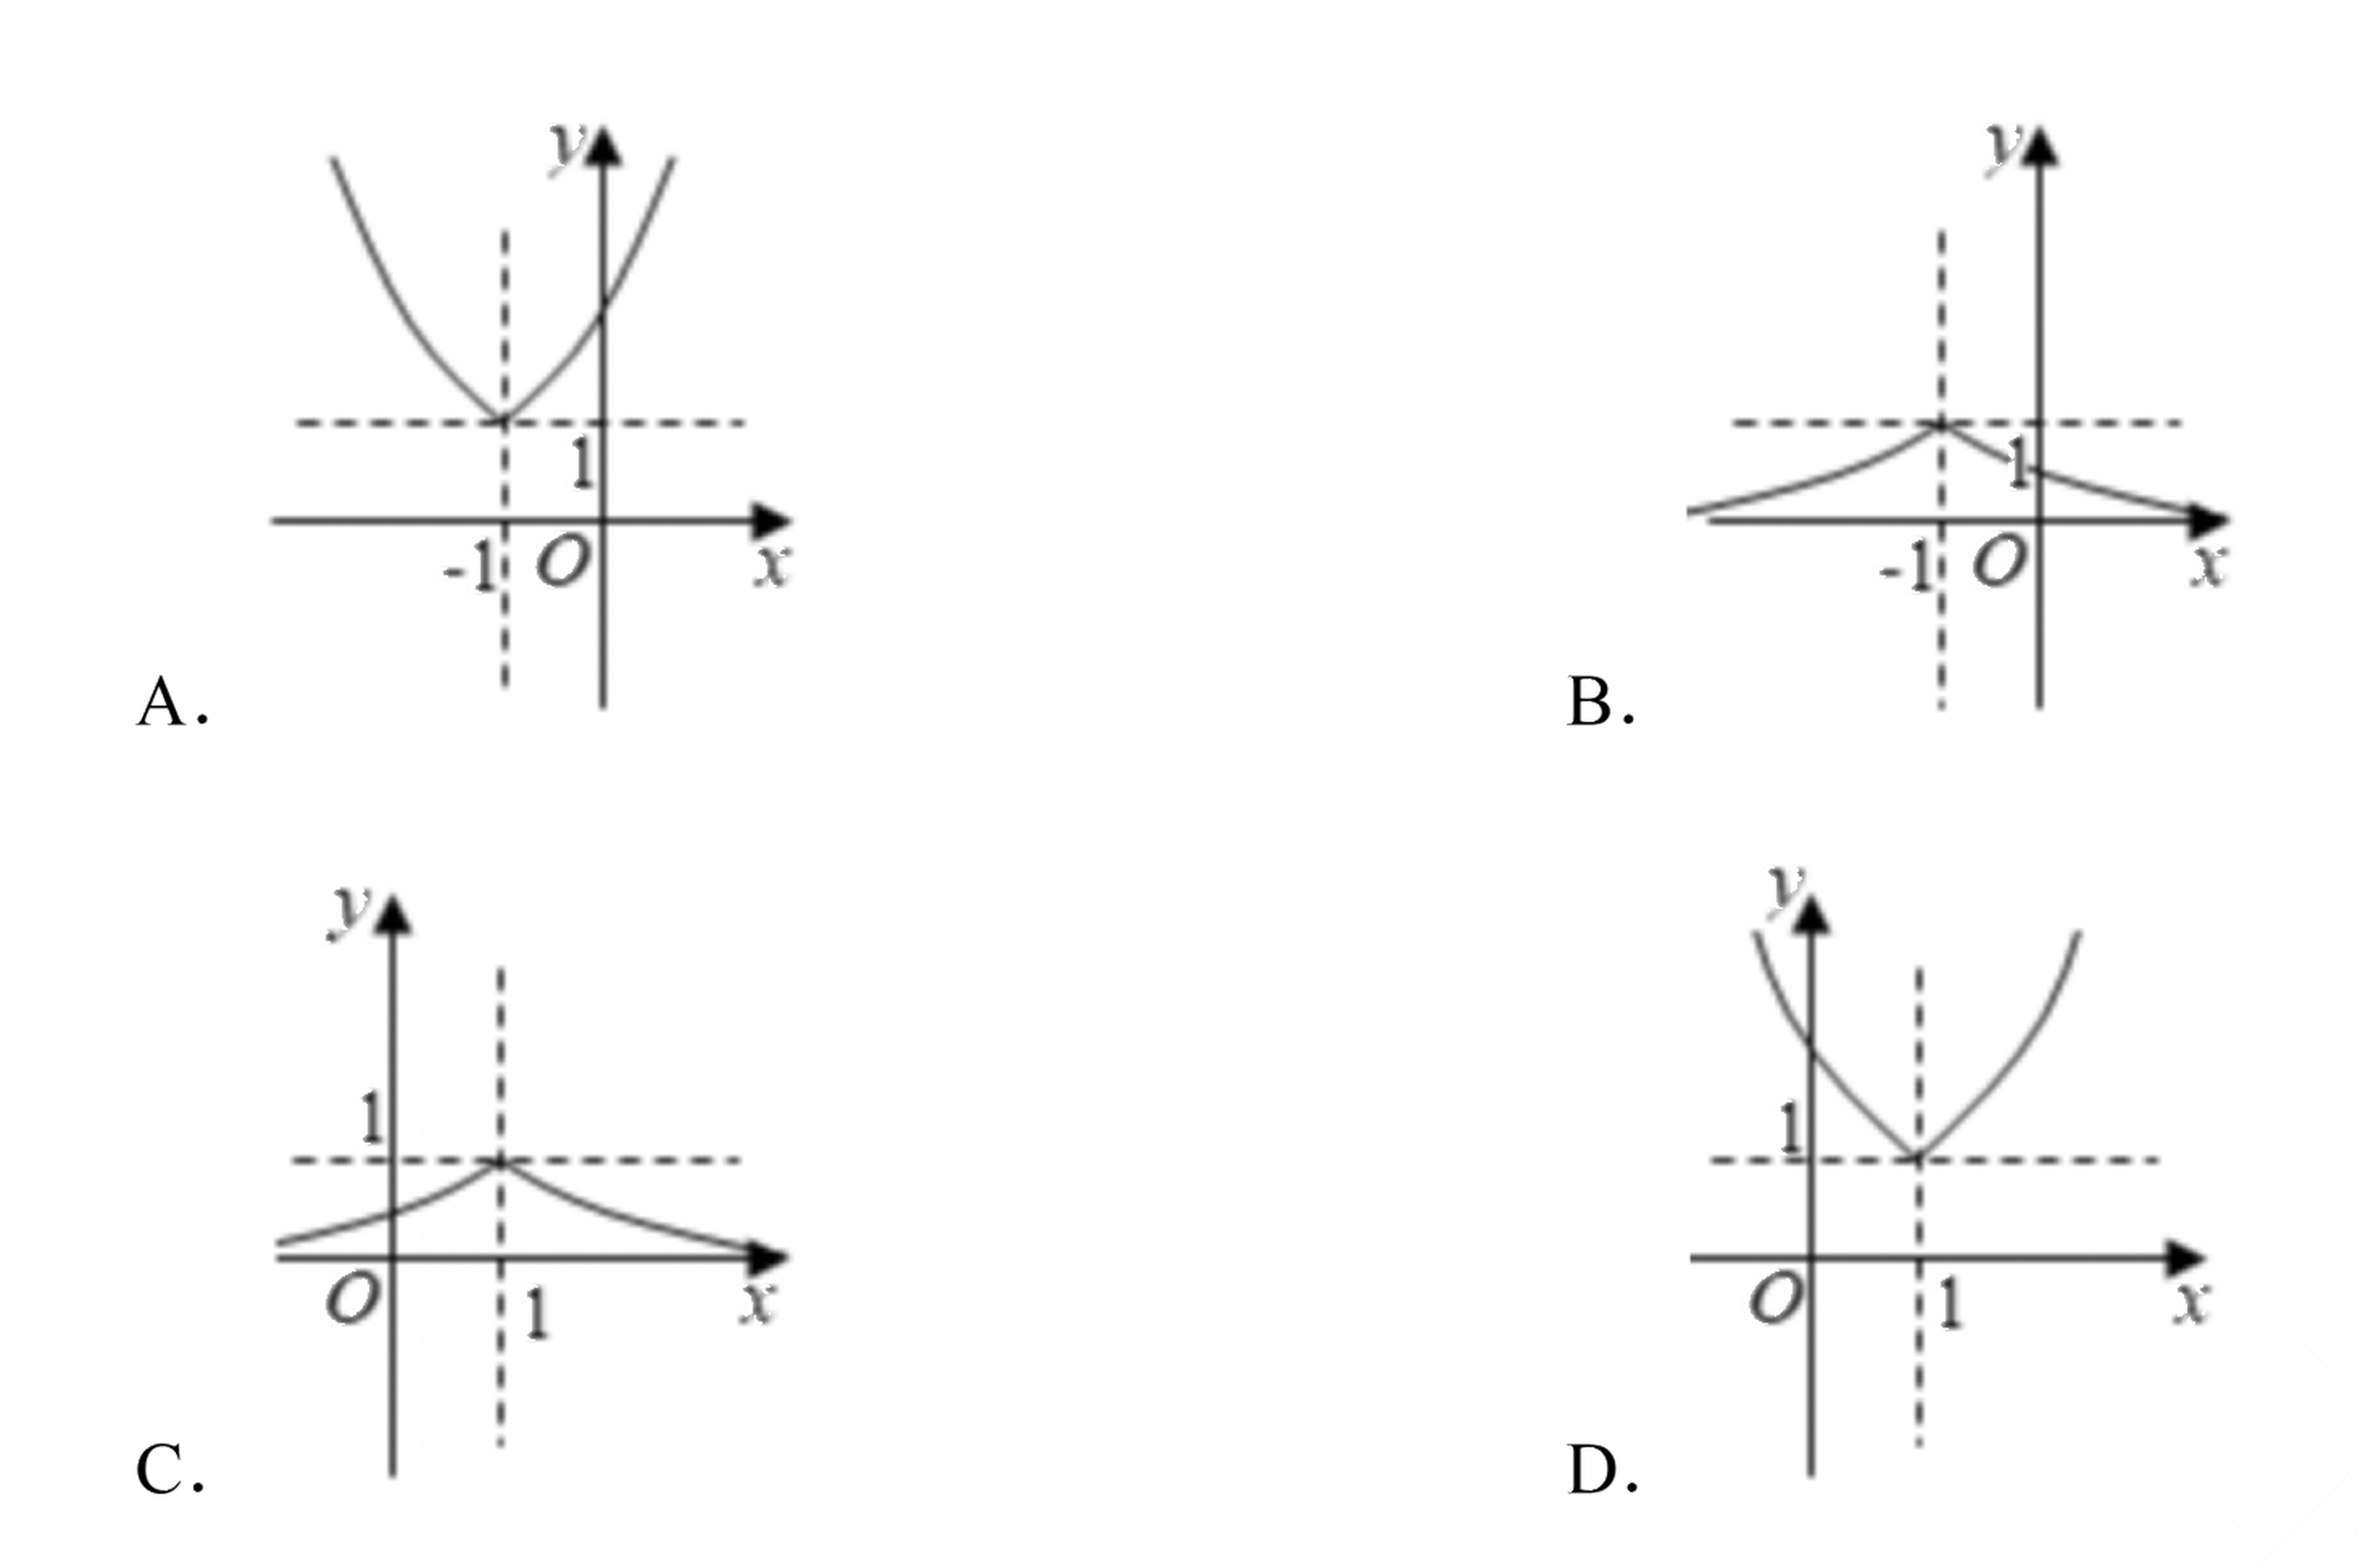
\includegraphics[width=0.80\textwidth]{figures/gao136_q22.png}
\end{center}

\ifanswer
\ans{$B$}
\fi

\end{enumerate}

\end{document}
"
%
% ① 原始材料：微信公众号"魔都数学加油站"文章，作者破晓，2026-11-15 18:04 发布；
% 连载"27学年高一136"，原文标题"27学年高一136——2026-2027年上海市三林中学高一上期中"；
% 原文链接：https://mp.weixin.qq.com/s/jaMzqMm6pDvcT0yM0d7eaQ。
% 正文为 7 张 PNG 页（01、04、06 为 4762x6735；02、03、05、07 为 2560x3620，
% 同一篇各页分辨率不同，逐页按各自分辨率裁图核对），题目下印有【答案】或【解析】，为讲评版。
% 题目、解析均据原图转录；卷面粉红色水印"魔都数学加油站"及公众号页脚未录入。
% 全卷 3 幅插图：第 13 题四幅坐标图选项（03 页）、第 20 题药物浓度折线/曲线图（05 页）、
% 第 22 题四幅抛物线/坐标图选项（07 页），均取原卷截图去粉色水印、去色、LANCZOS 放大，
% 四幅选项按原卷 2x2 排布合并为一张；图前按惯例加 \needvspace 守卫。
%
% 卷首标题：原卷印作"2026-2027 年三林中学高一上期中"（公众号标题中的"上海市"
% 卷面标题行没有，本稿照卷面），年份区间按全稿惯例排 en dash；原卷未印副标题，
% 本卷为期中卷、跨集合与常用逻辑用语／不等式／函数三章，按题目内容标为
% "集合与常用逻辑用语、不等式、函数"（与 125／126／128／129／131／132／133 同期中卷口径相同）：
% 集合与逻辑见 Q3、Q6、Q10、Q12、Q16、Q18、Q21，不等式见 Q5、Q7、Q8、Q9、Q14、Q15，
% 函数（幂函数、指数／对数、基本不等式应用）见 Q4、Q11、Q13、Q17、Q19、Q20、Q22。
%
% 题号体例：本卷共 20 题——一、填空题 3—12（10 题）、二、选择题 13—16（4 题）、
% 三、解答题 17—21（5 题）、四、附加题 22（1 题）。四节分别
% \setcounter{enumi}{2}／{12}／{16}／{21}。
%
% ② 与原卷的排版差异：
%   ① 原文从第 3 题起，本稿保留原题号；末节"四、附加题"另起 \bigsec，题号续到 22；
%   ② 原卷每题下直接印【答案】或【解析】，本稿按全稿惯例置于答案版；第 3、4、6 题只印
%      【答案】、无【解析】，提 \ans{}；第 14 题答案 C 印在题干括号内、无【解析】，按
%      高一53／高一108／高一132／高一133 成例括号留空、另提 \ans{$C$}；第 22 题答案 B
%      印在题干括号内、无【解析】，同例提 \ans{$B$}；第 13、15、16 题答案在解析末句
%      "故选 …"，括号内留空、不另提 \ans{}；其余各题印【解析】、无独立答案段；
%   ③ 原卷未印副标题，本稿按"知识模块"口径补出；
%   ④ 原卷填空横线按全稿惯例排为 \blankline[4.4em]；选择题括号排 \mbox{（\quad）}、
%      每个选项段前按惯例加 \keepwithprev（四幅图选项那一枚放在 \begin{center} 之前）；
%      解答题不留作答区、不加 \anspace（原卷为讲评版，与 129／131／132／133 同）；
%   ⑤ 原卷数集排斜体 $R$／$R^+$／$Z$，按全稿惯例改 \R／\R^+／\Z；空集记号 \varnothing；
%      绝对值排 \lvert…\rvert，集合描述竖线排 \mid；不等号按全稿惯例排 \leqslant／\geqslant；
%   ⑥ 子题标号 (1)(2)(3) 原卷用半角括号，照录；圈数字 ①②③④ 照录；第 12 题甲／乙／丙
%      三行与第 14 题四个编号不等式照录；
%   ⑦ 数学式内半角逗号照录（如 Q4"$a>0,a\neq1$"、Q6"$\{(-2,4),(1,1)\}$"、
%      Q7"$a=2+3=5,b=2\times3=6$"、Q11"$x_1,x_2$"、Q12"$m,n\in R^+$"、
%      Q15"$a>1,b\geq0$"、Q18"$B=(2a,a+1)$"、Q20"$4t,0\leq t\leq1$"、
%      Q21"$\{-3,-2,-1,0,1,2,3\}$"）；原卷行末西文句点照录，行中全角逗号照录；
%   ⑧ 三幅插图：第 13 题四幅坐标图选项合并裁为一张 \includegraphics（题前 \needvspace{9cm}）；
%      第 20 题折线/曲线图取 05 页截图（0.42\textwidth）；第 22 题四幅抛物线/坐标图选项合并
%      裁为一张（题前 \needvspace{9cm}）。第 13、22 题分别是"二、选择题""四、附加题"的首题
%      且带大图块，另在两处 \bigsec 之前各加 \needvspace{11cm} 连节标题一起量，避免节标题
%      孤立在页末（切页审计 B 类；照 高一26／40／59 成例）。第 20 题图不是节首题、三版试排
%      图均与题干同页，加 7cm 守卫反会多出一张只有两行正文的稀疏页，故不另加守卫；
%      三版切页审计均"合计异常：无"（试卷 4 页／紧凑 4 页／答案 6 页）；
%   ⑨ 跨页续印按题合并：Q16 题干在 03 页、括号与选项及【解析】在 04 页；Q19 题干在 04 页、
%      (2) 与【解析】在 05 页；Q20 (3)【解析】在 06 页；Q22 四幅图在 07 页；本稿按题连排；
%   ⑩ 题干中的中文弯引号按原卷照录，注释内一律 ASCII 引号；原卷"图像／图象"两种写法混用，
%      逐处照录（Q4、Q19 作"图像"，Q13、Q15、Q20、Q22 作"图象"）；
%   ⑪ 附加题节：原卷印"四、附加题"，本稿用 \bigsec{四、附加题} 另起一节、
%      \setcounter{enumi}{21}，顶层 1 个 \item（与 高一09／15／16／22／35／39／47／61 同口径）；
%      Q22 只印括号内答案、提 \ans{}，不计入 \step 账。
%
% 判别式字形：全卷仅第 9 题【解析】cases 块出现判别式"$\Delta=a^2-8a<0$"，原卷印
%   等腰、偏高的三角 $\Delta$，逐处放大核对并照录 \Delta；全卷未出现扁等边三角 \triangle。
%
% 子集符号：第 18 题 (2) 题干"$B\subseteq A$"与【解析】"$B\subseteq A$"两处原卷均印
%   带下划线 $\subseteq$，逐处放大核对、照录 \subseteq；全卷未出现单线 \subset。
%
% 原卷存疑照录（均照录未改，正文对应处另有 % 注）：
%   第 12 题乙行"$\dfrac{m+n}{mm}=\dfrac1{mn}$"前一分母印作 $mm$（后一处作 $mn$），照录；
%   第 12 题【解析】"$\geqslant\dfrac1{100}\left[a^2+1+2\sqrt{a^2}\right]$"保留 $\sqrt{a^2}$
%      未化简为 $a$，照录；
%   第 13 题【解析】"排除 BC"与"排除 D"连写选项字母，照录；
%   第 18 题 (2)【解析】末行"所以实数 $a$ 的取值范围 $(-\infty,-2]\cup[\frac12,1)$"
%      "取值范围"后脱"是／为"字，照录；
%   第 21 题 (3) 题干"求出使得集合 $B$ 中元素最少的 $k$ 的所有取值"而【解析】只给出
%      $k=-2$ 一处，措辞照录。
%
% 行数复核：逐题数 \step 条数，合计 51 条（Q3：0；Q4：0；Q5：2；Q6：0；Q7：2；Q8：1；
% Q9：1；Q10：4；Q11：1；Q12：4；Q13：2；Q14：0；Q15：2；Q16：3；Q17：1；Q18：5；
% Q19：4；Q20：7；Q21：12；Q22：0），与原卷印刷行逐题相等（cases 块作一个印刷行计）。
% 第 3、4、6、14、22 题只印【答案】、提 \ans{}，不计入 \step 账；第 13、15、16 题答案在
% 解析末句，括号内留空、不另提 \ans{}。
%
\documentclass[a4paper,11pt]{article}
\usepackage{common}

\begin{document}

\examtitlest[3]{2026--2027 年三林中学高一上期中}{集合与常用逻辑用语、不等式、函数}

\bigsec{一、填空题}

\begin{enumerate}
\setcounter{enumi}{2}

\item 用反证法证明命题“若 $x+y\neq5$，则 $x\neq2$ 或 $y\neq3$”为真命题时，第一个步骤是\blankline[4.4em].

\ifanswer
\ans{假设 $x=2$ 且 $y=3$}
\fi

\item 函数 $y=a^{x-1}+1(a>0,a\neq1)$ 的图像恒过定点 $A$，则点的坐标是\blankline[4.4em].

\ifanswer
\ans{$(1,2)$}
\fi

\item 已知 $x>1$，则 $x+\dfrac4{x-1}$ 的最小值是\blankline[4.4em].

\ifanswer
\solbegin
\step{由 $x>1$，得 $x-1>0$，则 $x+\dfrac4{x-1}=x-1+\dfrac4{x-1}+1\geqslant2\sqrt{(x-1)\cdot\dfrac4{x-1}}+1=5$，}
\step{当且仅当 $x-1=\dfrac4{x-1}$ 即 $x=3$ 时取等号，取得最小值 $5$.}
\solend
\fi

\item 已知集合 $A=\{(x,y)\mid y=x^2\}$，集合 $B=\{(x,y)\mid y=2-x\}$，求 $A\cap B=$\blankline[4.4em].

\ifanswer
\ans{$\{(-2,4),(1,1)\}$}
\fi

\item 已知一元二次不等式 $x^2-ax+b<0$ 的解集为 $(2,3)$，则不等式 $bx^2-ax+1>0$ 的解集是\blankline[4.4em].

\ifanswer
\solbegin
\step{$a=2+3=5,b=2\times3=6$，则 $bx^2-ax+1>0$ 即 $6x^2-5x+1>0$，}
\step{即 $(3x-1)(2x-1)>0$，解集为 $\left(-\infty,\dfrac13\right)\cup\left(\dfrac12,+\infty\right)$.}
\solend
\fi

\item 不等式 $(x+2)^3<(5-2x)^3$ 的解集为\blankline[4.4em].

\ifanswer
\solbegin
\step{由 $(x+2)^3<(5-2x)^3$ 得 $x+2<5-2x$，故解集为 $(-\infty,1)$.}
\solend
\fi

\item 若关于 $x$ 的不等式 $ax^2-ax+2>0$ 的解集为 $\R$，则实数 $a$ 的取值范围是\blankline[4.4em].

\ifanswer
\solbegin
\step{由题意得 $a=0$ 或 $\begin{cases}a>0\\\Delta=a^2-8a<0\end{cases}$，所以 $0\leqslant a<8$.}% 判别式原卷印高三角 $\Delta$，照录
\solend
\fi

\item 已知关于 $x$ 的不等式 $\lvert x+3\rvert+\lvert x-a\rvert\geqslant5$ 恒成立，则实数 $a$ 的取值范围为\blankline[4.4em].

\ifanswer
\solbegin
\step{因为 $\lvert x+3\rvert+\lvert x-a\rvert\geqslant\lvert x-a-x-3\rvert=\lvert 3+a\rvert$，}
\step{要使 $\lvert x+3\rvert+\lvert x-a\rvert\geqslant5$ 恒成立，则 $\lvert a+3\rvert\geqslant5$ 即可，}
\step{所以 $a+3\geqslant5$ 或 $a+3\leqslant-5$，解得 $a\geqslant2$ 或 $a\leqslant-8$，}
\step{即实数 $a$ 的取值范围是 $(-\infty,-8]\cup[2,+\infty)$.}
\solend
\fi

\item 若方程 $\lg^2 x-2\lg x-2=0$ 的两个解为 $x_1,x_2$，求 $\log_{x_1}x_2+\log_{x_2}x_1$ 的值为\blankline[4.4em].

\ifanswer
\solbegin
\step{$\log_{x_1}x_2+\log_{x_2}x_1=\dfrac{\lg x_2}{\lg x_1}+\dfrac{\lg x_1}{\lg x_2}=\dfrac{(\lg x_1+\lg x_2)^2-2\lg x_1\lg x_2}{\lg x_1\lg x_2}=-4$.}
\solend
\fi

\item 三个同学对问题“已知 $m,n\in \R^+$，且 $m+n=1$，求 $\dfrac1m+\dfrac1n$ 的最小值”提出各自的解题思路：

思路：

甲：$\dfrac1m+\dfrac1n=\dfrac{m+n}{m}+\dfrac{m+n}{n}=2+\dfrac nm+\dfrac mn$，可用基本不等式求解；

乙：$\dfrac1m+\dfrac1n=\dfrac{m+n}{mm}=\dfrac1{mn}=\dfrac1{m(1-m)}$，可用二次函数配方法求解；% 原卷前一分母印作 $mm$，照录

丙：$\dfrac1m+\dfrac1n=\left(\dfrac1m+\dfrac1n\right)(m+n)=2+\dfrac nm+\dfrac mn$，可用基本不等式求解；参考上述解题思路，

可求得当 $x=$\blankline[4.4em]时，$y=\dfrac{a^2}{x^2}+\dfrac1{100-x^2}$（$0<x<10$，$a>0$）有最小值.

\ifanswer
\solbegin
\step{$y=\dfrac{a^2}{x^2}+\dfrac1{100-x^2}=\left(\dfrac{a^2}{x^2}+\dfrac1{100-x^2}\right)[x^2+(100-x^2)]\times\dfrac1{100}$}
\step{$=\dfrac1{100}\left[a^2+1+\dfrac{x^2}{100-x^2}+\dfrac{a^2(100-x^2)}{x^2}\right]\geqslant\dfrac1{100}\left[a^2+1+2\sqrt{a^2}\right]$}% 原卷保留 $\sqrt{a^2}$ 未化简，照录
\step{当且仅当 $\dfrac{x^2}{100-x^2}=\dfrac{a^2(100-x^2)}{x^2}$，即 $x=\sqrt{\dfrac{100a}{a+1}}$ 时，}
\step{$y=\dfrac{a^2}{x^2}+\dfrac1{100-x^2}(0<x<10,a>0)$ 有最小值.}
\solend
\fi

\end{enumerate}

% 第 13 题是"二、选择题"首题且带 9cm 图块，守卫须放在 \bigsec 之前连节标题一起量，
% 否则"二、选择题"会孤立在页末（B 类，照 高一26／40／59 成例）
\needvspace{11cm}
\bigsec{二、选择题}

\begin{enumerate}
\setcounter{enumi}{12}

% 第 13 题四幅坐标图选项是一整块，守卫放在 \item 之前
\needvspace{9cm}
\item 下列图象中，最符合函数 $y=x^{\frac54}$ 的图象的是\mbox{（\quad）}

\keepwithprev
\begin{center}
% 四幅坐标图选项取原卷 03 页截图去粉色水印，按原卷 2x2 排布合并为一张
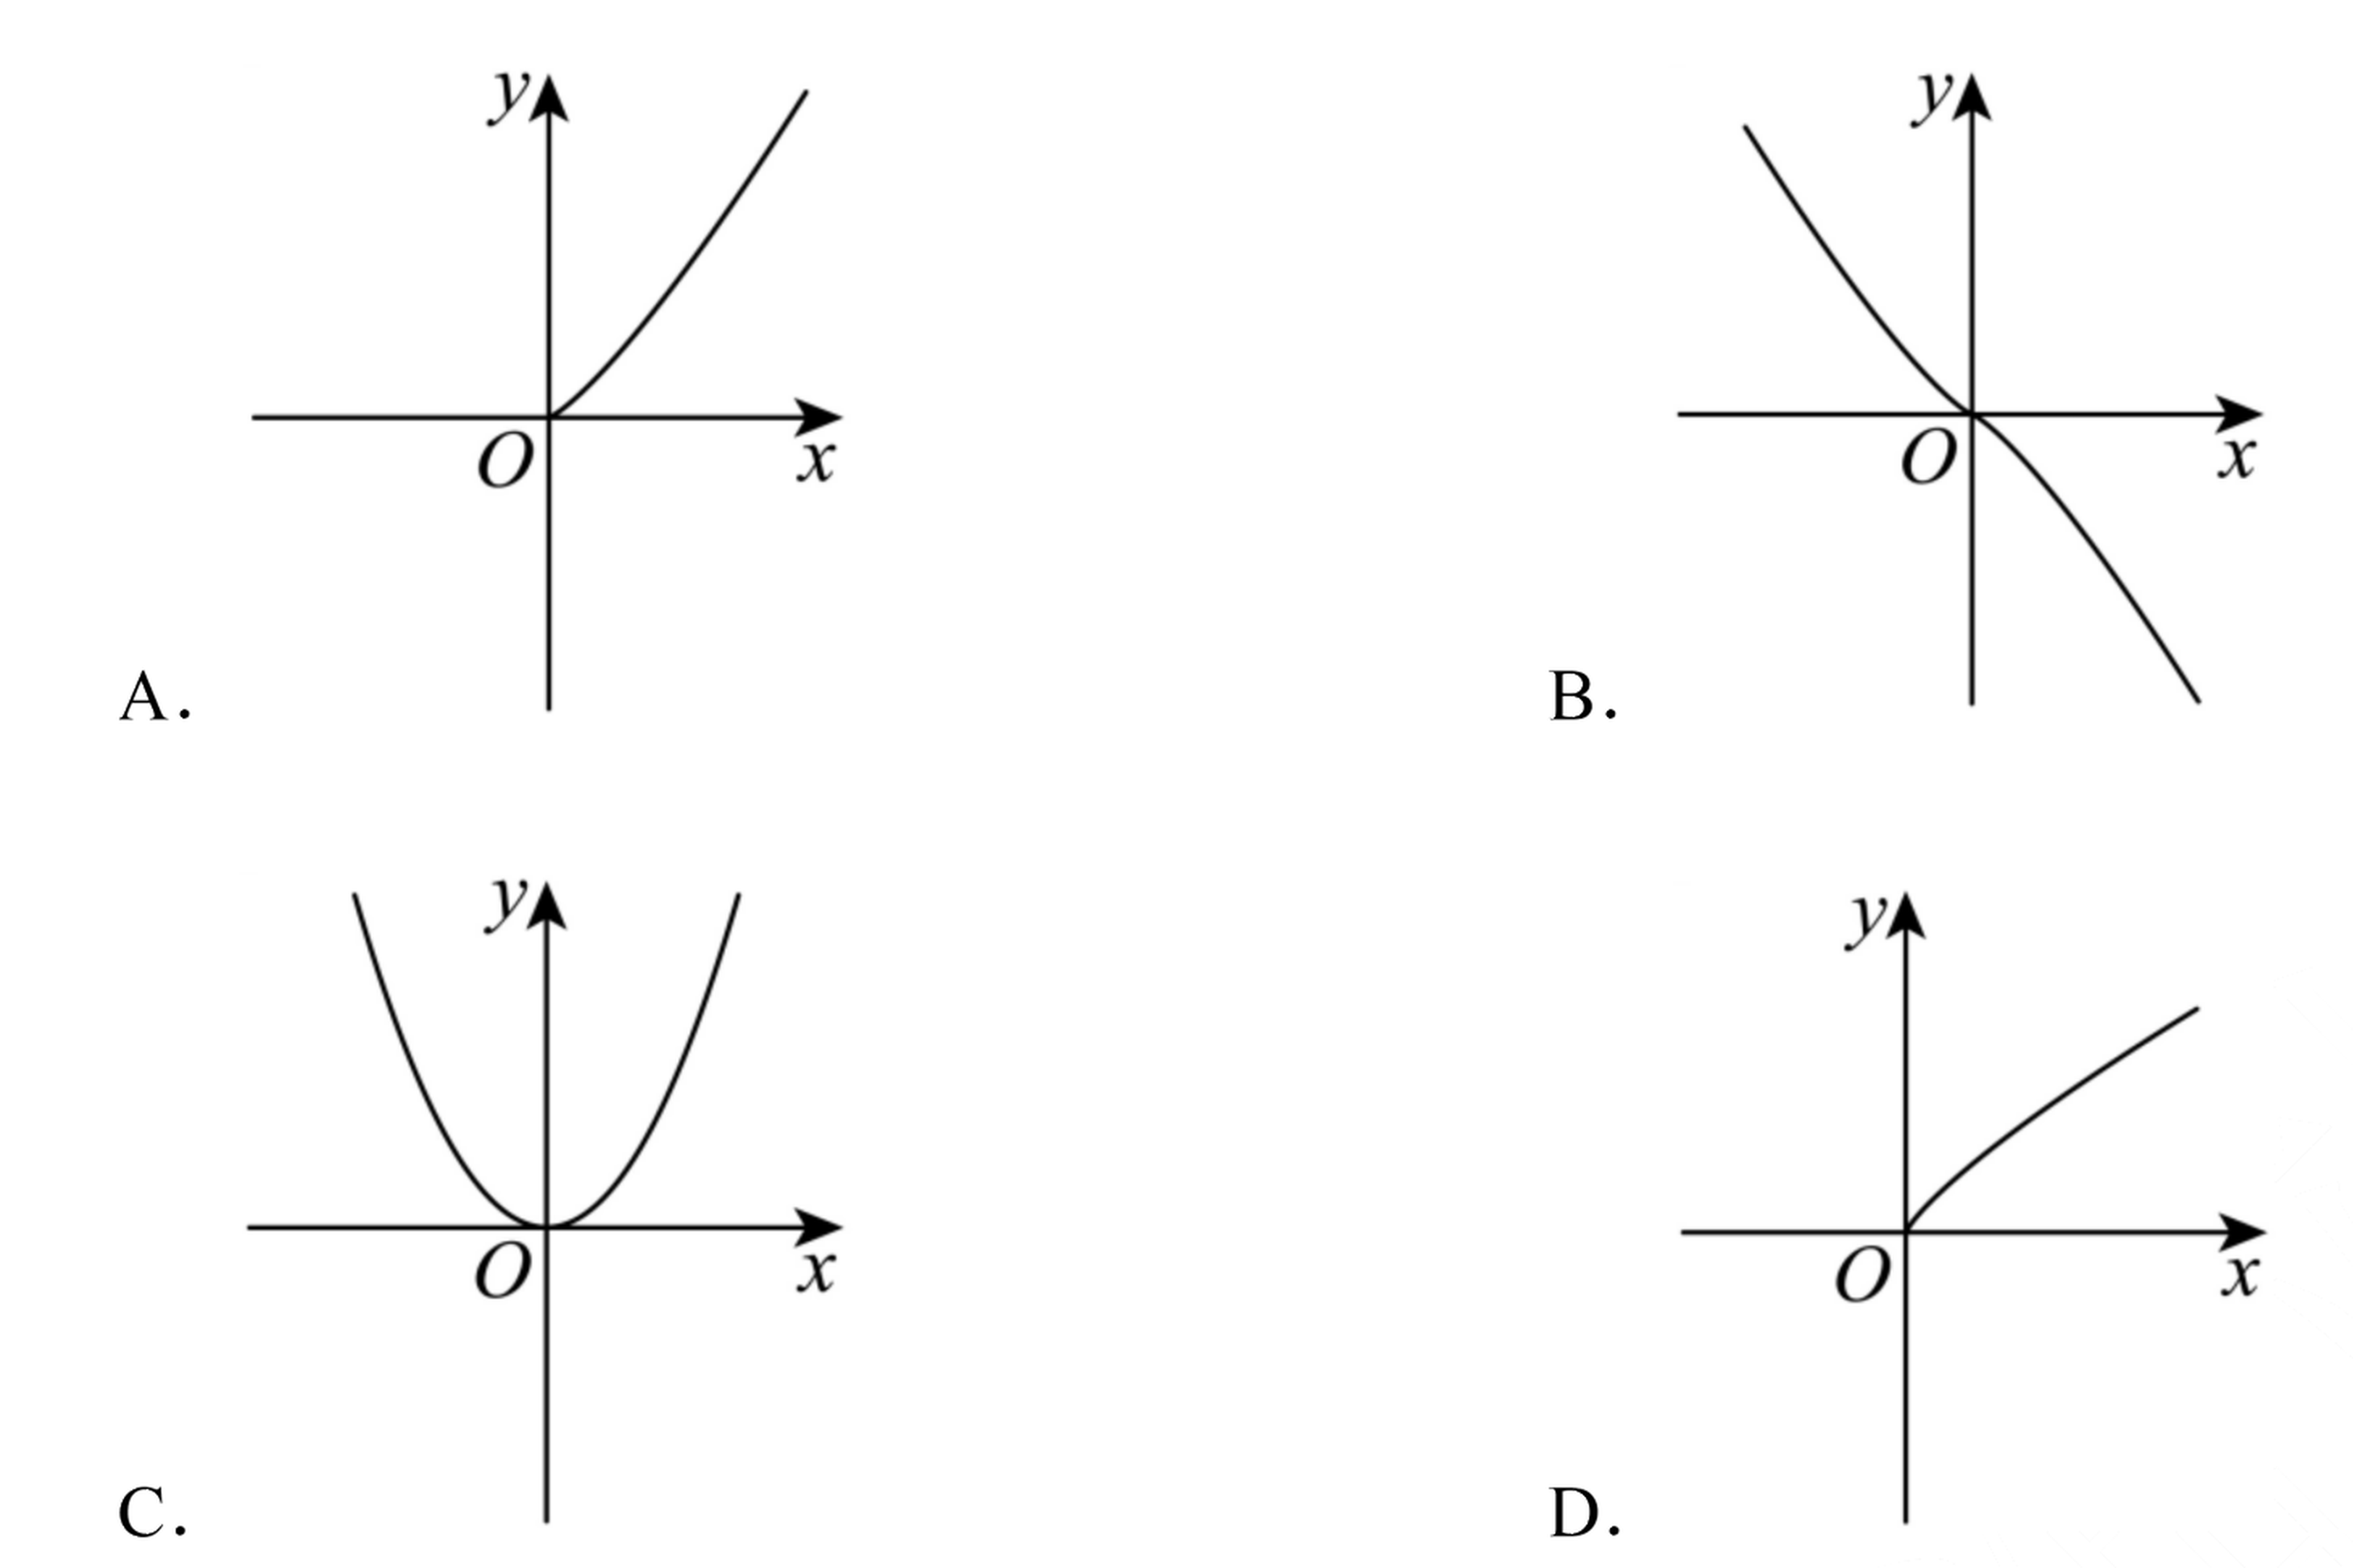
\includegraphics[width=0.80\textwidth]{figures/gao136_q13.png}
\end{center}

\ifanswer
\solbegin
\step{由 $y=x^{\frac54}=\sqrt[4]{x^5}$，函数的定义域为 $[0,+\infty)$，排除 BC，}% 原卷"排除 BC"连写，照录
\step{因为 $\dfrac54>1$，所以函数 $y=x^{\frac54}$ 的图象呈现下凸的趋势，排除 D. 故选 $A$.}
\solend
\fi

\item 下列不等式① $a+\dfrac1a\geqslant2$；② $a^2+4\geqslant4a$；③ $\left\lvert\dfrac ba+\dfrac ab\right\rvert\geqslant2$；④ $\dfrac{2a^2b^2}{a^2+b^2}\leqslant ab$；其中恒成立的是\mbox{（\quad）}

\keepwithprev
A. ①④\qquad B. ③④\qquad C. ②③\qquad D. ①②

\ifanswer
\ans{$C$}
\fi

\item 函数 $y=a^x+b-1(a>0,a\neq1)$ 单调递增且图象不经过第四象限，则 $a,b$ 满足的条件为\mbox{（\quad）}

\keepwithprev
A. $a>1,b\leqslant1$\qquad B. $a>1,b\geqslant0$\qquad C. $0<a<1,b\leqslant1$\qquad D. $0<a<1,b\geqslant1$

\ifanswer
\solbegin
\step{因为函数 $y=a^x+b-1$ 单调递增，所以 $a>1$，}
\step{图象不经过第四象限，则 $x=0$ 时，$y=b\geqslant0$，所以 $a>1,b\geqslant0$，故选 $B$.}
\solend
\fi

\item 设关于 $x$ 的不等式 $\dfrac{ax-1}{x^2-a}<0$ 的解集为 $S$，且 $3\in S$，$4\notin S$，则实数 $a$ 的取值范围为\mbox{（\quad）}

\keepwithprev
A. $(-\infty,-\sqrt3)\cup\left(\dfrac13,\sqrt3\right)$\qquad B. $\left(-\infty,\dfrac14\right)\cup(16,+\infty)$

C. $\left[\dfrac14,\dfrac13\right)\cup(9,16]$\qquad D. 不能确定

\ifanswer
\solbegin
\step{若 $3\in S$，则 $\dfrac{3a-1}{9-a}<0$，解得 $a\in\left(-\infty,\dfrac13\right)\cup(9,+\infty)$，}
\step{若 $4\notin S$，则 $16-a=0$ 或 $\dfrac{4a-1}{16-a}\geqslant0$，解得 $a\in\left[\dfrac14,16\right]$，}
\step{故实数 $a$ 的取值范围为 $\left[\dfrac14,\dfrac13\right)\cup(9,16]$，故选 $C$.}
\solend
\fi

\end{enumerate}

\bigsec{三、解答题}

\begin{enumerate}
\setcounter{enumi}{16}

\item 计算：(1) 计算 $\dfrac{\lg8+\lg125-\lg2-\lg5}{\lg\sqrt{10}\cdot\lg0.1}$；(2) 若 $a^{2x}=2(a>0)$，求 $\dfrac{a^{3x}+a^{-3x}}{a^x+a^{-x}}$.

\ifanswer
\solbegin
\step{(1) 原式 $=\dfrac{2-1}{\frac12\cdot(-1)}=-2$；(2) 原式 $=a^{2x}-1+a^{-2x}=2-1+\dfrac12=\dfrac32$.}
\solend
\fi

\item 不等式 $\dfrac{x-1}{x+1}\geqslant0$ 的解集为 $A$，不等式 $(x-a-1)(2a-x)>0(a<1)$ 的解集为 $B$.

(1) 求集合 $A$；

(2) 若 $B\subseteq A$，求实数 $a$ 的取值范围.

\ifanswer
\solbegin
\step{(1) $A=(-\infty,-1)\cup[1,+\infty)$.}
\step{(2) 由 $(x-a-1)(2a-x)>0(a<1)$，得 $(x-a-1)(x-2a)<0(a<1)$，}
\step{因为 $a<1$，所以 $a+1>2a$，所以 $B=(2a,a+1)$，}
\step{因为 $B\subseteq A$，所以 $2a\geqslant1$ 或 $a+1\leqslant-1$，即 $a\geqslant\dfrac12$ 或 $a\leqslant-2$，}
\step{而 $a<1$，所以实数 $a$ 的取值范围 $(-\infty,-2]\cup\left[\dfrac12,1\right)$.}% 原卷"取值范围"后脱"是／为"，照录
\solend
\fi

\item 已知幂函数 $y=x^m(m\in\R)$ 经过点 $\left(4,\dfrac12\right)$.

(1) 求此幂函数的表达式和定义域；

(2) 已知点 $A(a+2,y_1)$，点 $B(3-2a,y_2)(a\in\R)$ 在此幂函数的图像上，且满足 $y_1<y_2$，求实数 $a$ 的取值范围.

\ifanswer
\solbegin
\step{(1) 幂函数 $y=x^m(m\in\R)$ 经过点 $\left(4,\dfrac12\right)$，所以 $4^m=\dfrac12\Rightarrow m=-\dfrac12$，}
\step{所以 $f(x)=x^{-\frac12}$，定义域为 $(0,+\infty)$.}
\step{(2) 由于函数 $f(x)$ 在其定义域 $(0,+\infty)$ 上严格减，}
\step{由 $y_1<y_2$，得 $a+2>3-2a\geqslant0\Rightarrow a\in\left(\dfrac13,\dfrac32\right]$.}
\solend
\fi

% 第 20 题图取 05 页截图（0.42\textwidth、高约 6cm）。试排 \item 前加 7cm 守卫会多出
% 一张只有两行正文的稀疏页，且三版不加守卫时图均与题干、【解析】同页，故不另加守卫
\item 某医药研究所开发一种抗甲流新药，如果成年人按规定的剂量服用，据监测：服药后每毫升血液中的含药量 $y$（微克）与时间 $t$（小时）之间近似满足如图所示的曲线.

(1) 结合图，求 $k$ 与 $a$ 的值；

(2) 写出服药后 $y$ 与 $t$ 之间的函数关系式 $y=f(t)$；

(3) 据进一步测定：每毫升血液中含药量不少于 $0.5$ 微克时治疗疾病有效，求服药一次治疗有效的时间范围？

\begin{center}
% 图取原卷 05 页截图去粉色水印、去色，3x LANCZOS 放大
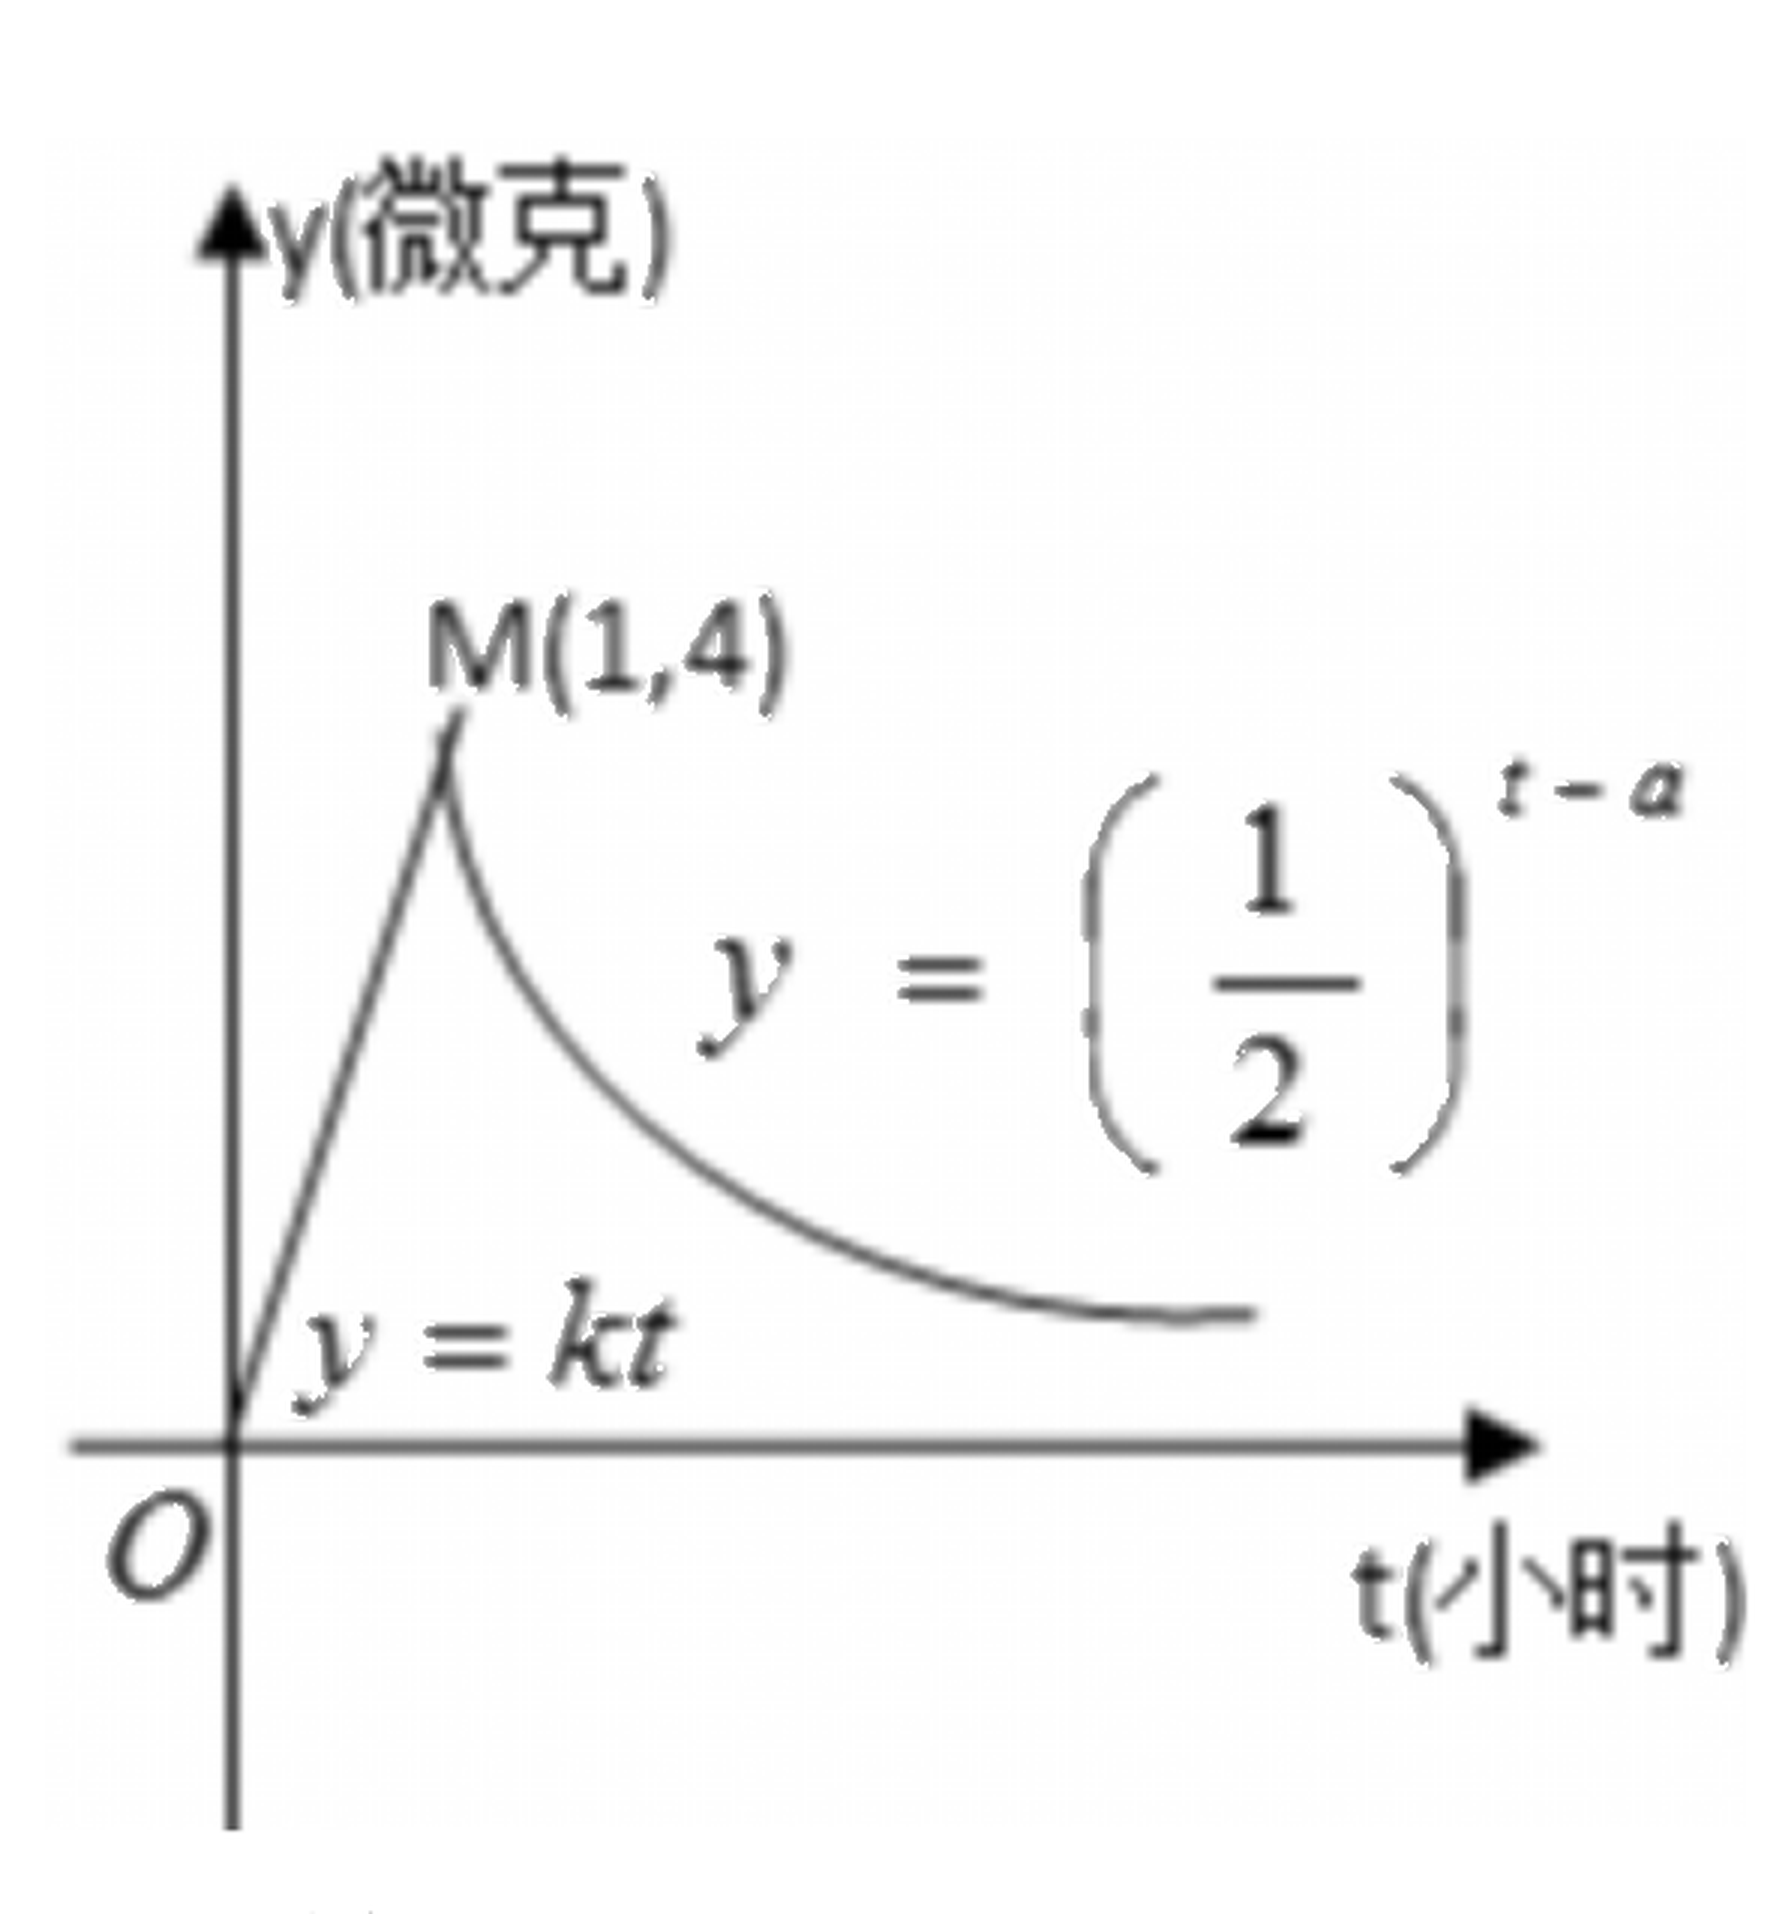
\includegraphics[width=0.42\textwidth]{figures/gao136_q20.png}
\end{center}

\ifanswer
\solbegin
\step{(1) 当 $0\leqslant t\leqslant1$ 时，函数图象是一条线段，由于过原点与点 $(1,4)$，所以 $k=4$，}
\step{其解析式为 $y=4t$，$0\leqslant t\leqslant1$；}
\step{当 $t\geqslant1$ 时，函数的解析式为 $y=\left(\dfrac12\right)^{t-a}$，}
\step{此时 $M(1,4)$ 在曲线上，将此点的坐标代入函数解析式得 $4=\left(\dfrac12\right)^{1-a}$，}
\step{解得 $a=3$；}
\step{(2) 由 (1) 得 $f(t)=\begin{cases}4t,0\leqslant t\leqslant1\\\left(\frac12\right)^{t-3},t>1\end{cases}$；}
\step{(3) 由 (2) 得，令 $f(t)\geqslant0.5$，即 $\begin{cases}4t\geqslant0.5,0\leqslant t\leqslant1\\\left(\frac12\right)^{t-3}\geqslant0.5,t>1\end{cases}$，所以 $\dfrac18\leqslant t\leqslant4$.}
\solend
\fi

\item 已知关于 $x$ 的不等式 $(kx-k^2-4)(x-4)>0$，其中 $k\in\R$.

(1) 当 $k=-1$，求不等式的解集 $A$；

(2) 当 $k$ 变化时，试求不等式的解集 $A$；

(3) 对于不等式解集 $A$，满足 $A\cap\Z=B$. 试探究集合 $B$ 能否为有限集，若能，求出使得集合 $B$ 中元素最少的 $k$ 的所有取值，并用列举法表示此时的集合 $B$，若不能，说明理由；

\ifanswer
\solbegin
\step{(1) 当 $k=-1$ 时，原不等式可化为 $(x+5)(x-4)<0$，}
\step{解得 $-5<x<4$，故不等式的解集为 $\{x\mid -5<x<4\}$；}
\step{(2) 当 $k=0$ 时，解集为 $\{x\mid x<4\}$，}
\step{当 $k>0$ 时，$\dfrac{k^2+4}{k}=k+\dfrac4k\geqslant4$，解集为 $\{x\mid x<4\text{ 或 }x>\dfrac{k^2+4}{k}\}$；}
\step{当 $k<0$ 时，解集为 $\{x\mid \dfrac{k^2+4}{k}<x<4\}$，}
\step{综上，当 $k=0$ 时，$A=\{x\mid x<4\}$，}
\step{当 $k>0$ 时，$A=\{x\mid x<4\text{ 或 }x>\dfrac{k^2+4}{k}\}$；}
\step{当 $k<0$ 时，$A=\{x\mid \dfrac{k^2+4}{k}<x<4\}$，}
\step{(3) 由 (2) 得当 $k\geqslant0$ 时，$B$ 为无限集，当 $k<0$ 时，$B$ 为有限集，}
\step{此时，$\dfrac{k^2+4}{k}=k+\dfrac4k\leqslant-4$，当且仅当 $k=-2$ 时取等号，}
\step{所以 $k=-2$ 时，$B$ 中元素最少，此时 $A=\{x\mid -4<x<4\}$，}
\step{所以 $B=\{-3,-2,-1,0,1,2,3\}$.}
\solend
\fi

\end{enumerate}

% 第 22 题是"四、附加题"首题且带 9cm 图块，守卫须放在 \bigsec 之前连节标题一起量，
% 否则"四、附加题"会孤立在页末（B 类，照 高一26／40／59 成例）
\needvspace{11cm}
\bigsec{四、附加题}

\begin{enumerate}
\setcounter{enumi}{21}

% 第 22 题四幅抛物线/坐标图选项是一整块，守卫放在 \item 之前
\needvspace{9cm}
\item 函数 $f(x)=\left(\dfrac12\right)^{\lvert x+1\rvert}$ 的图象大致为\mbox{（\quad）}

\keepwithprev
\begin{center}
% 四幅抛物线/坐标图选项取原卷 07 页截图去粉色水印，按原卷 2x2 排布合并为一张
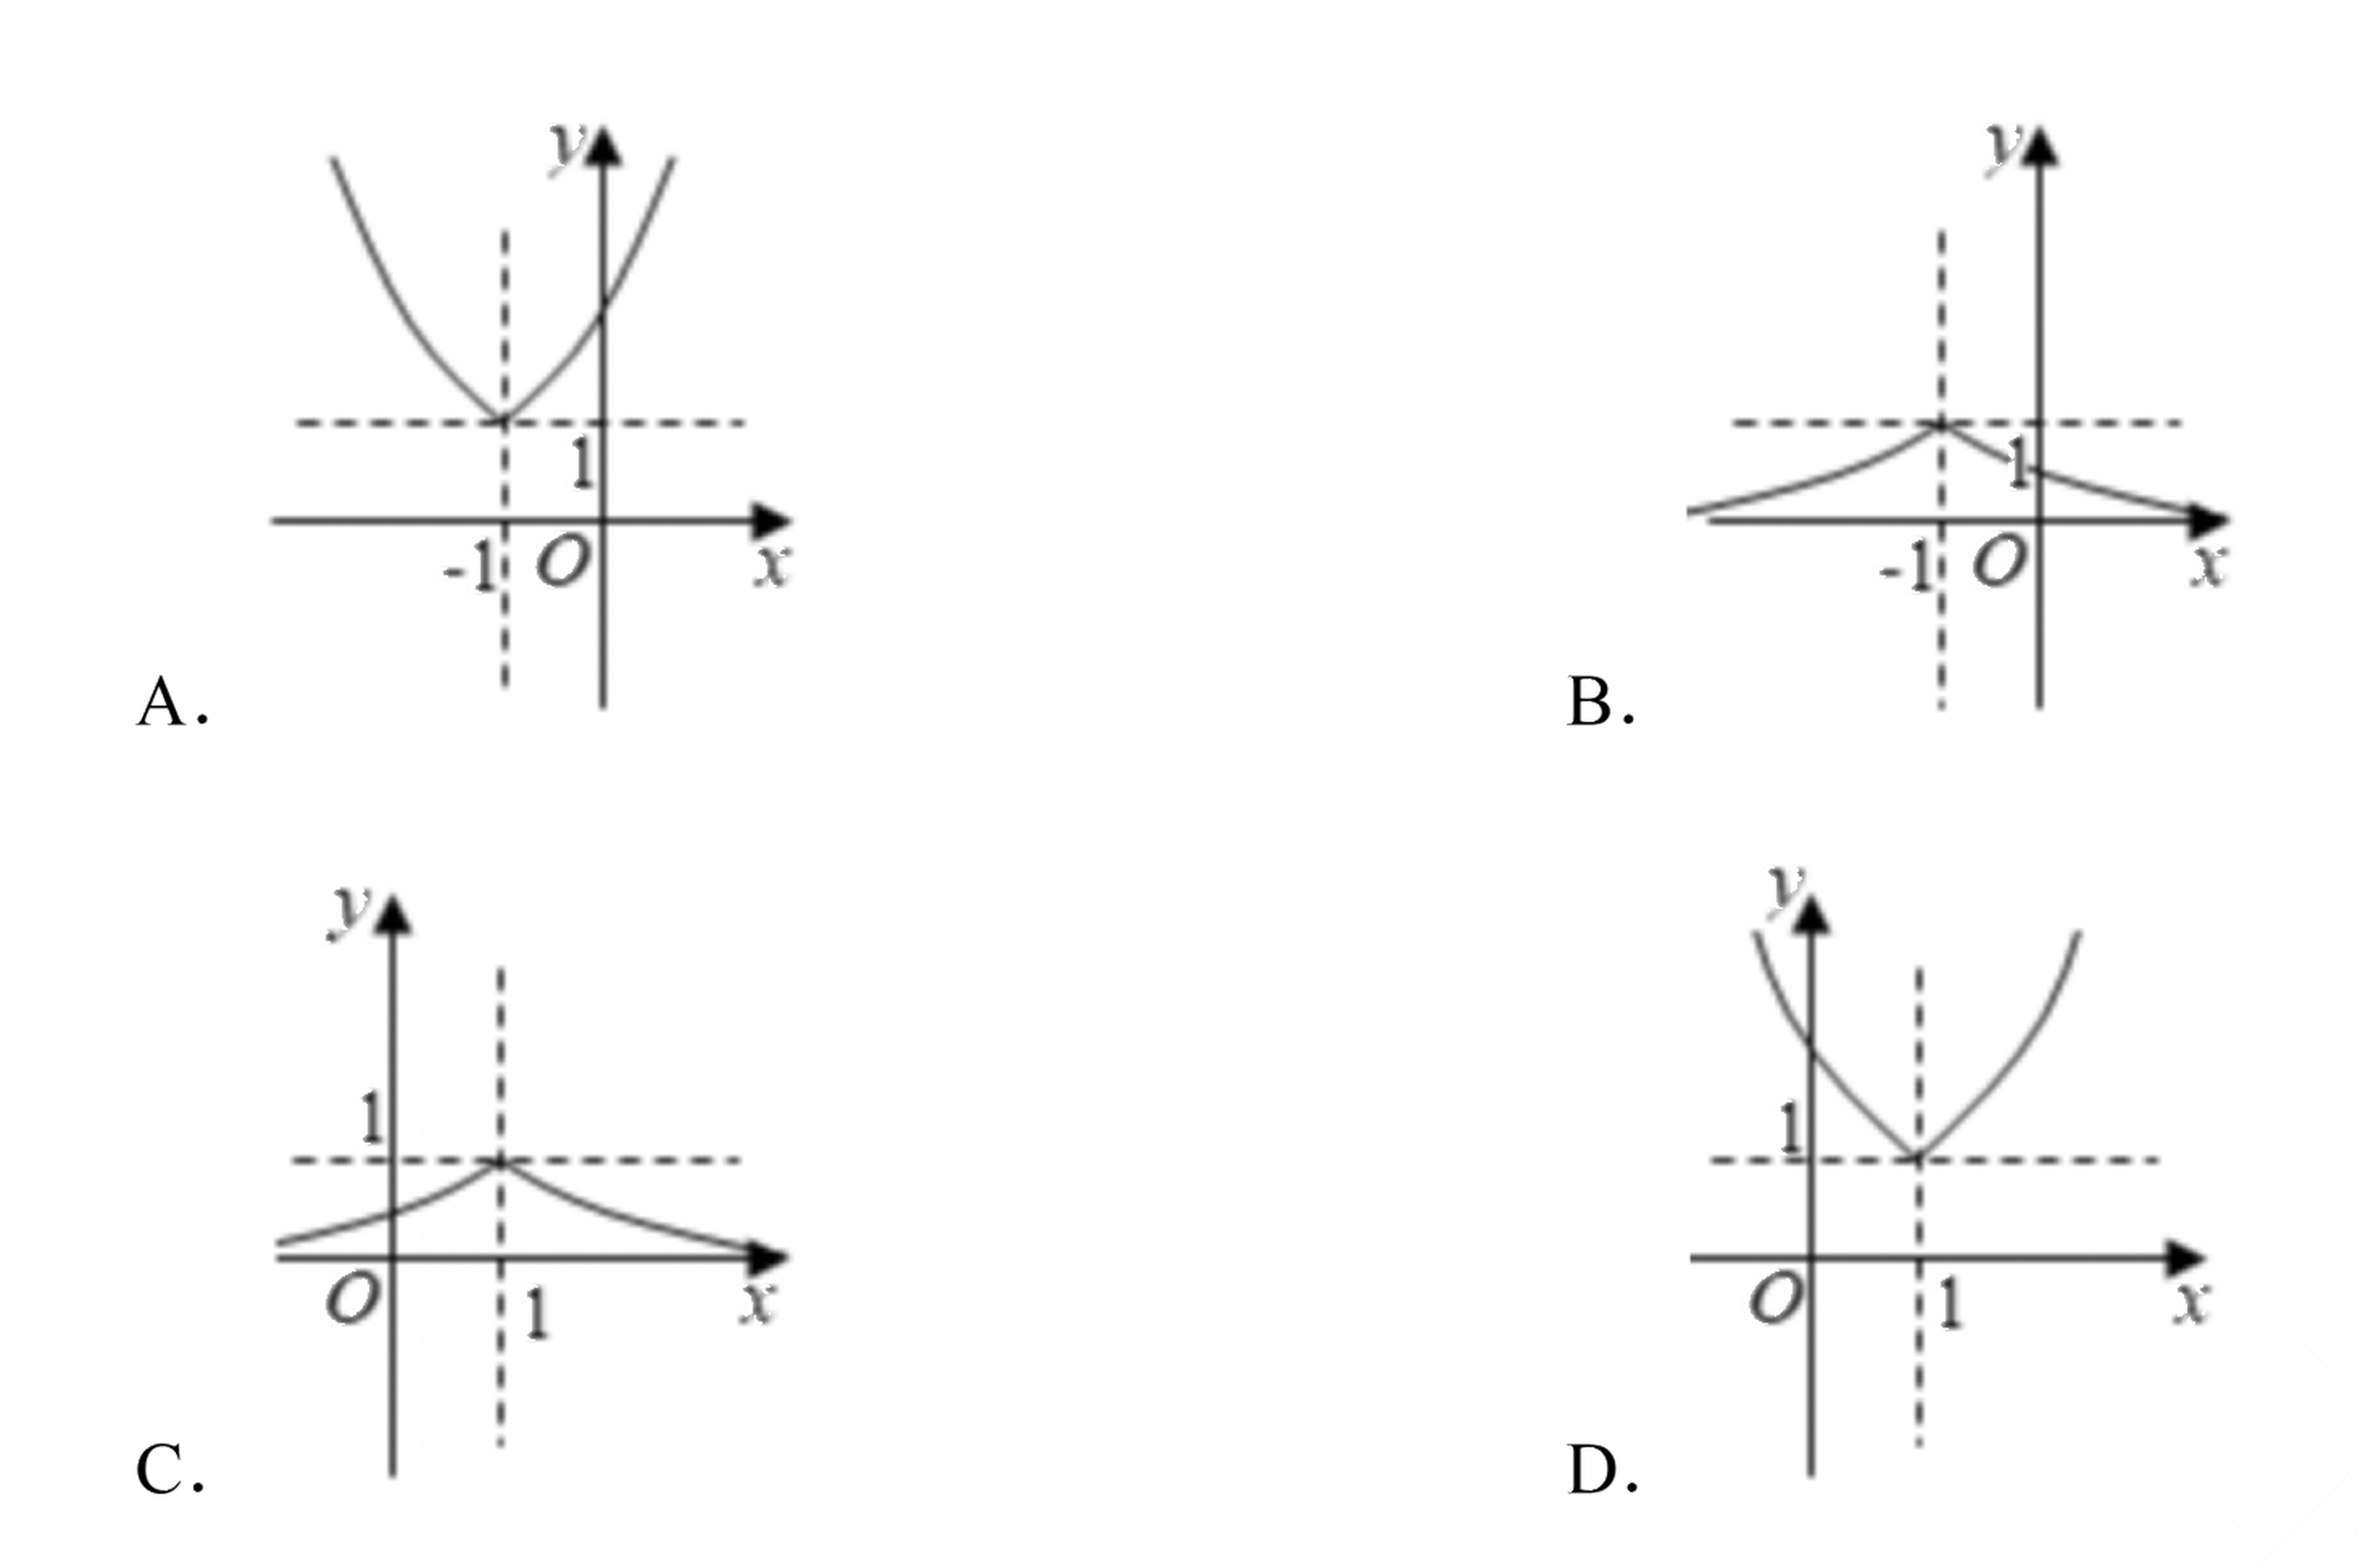
\includegraphics[width=0.80\textwidth]{figures/gao136_q22.png}
\end{center}

\ifanswer
\ans{$B$}
\fi

\end{enumerate}

\end{document}
